\documentclass[twoside]{book}

% Packages required by doxygen
\usepackage{calc}
\usepackage{doxygen}
\usepackage{graphicx}
\usepackage[utf8]{inputenc}
\usepackage{makeidx}
\usepackage{multicol}
\usepackage{multirow}
\usepackage{fixltx2e}
\PassOptionsToPackage{warn}{textcomp}
\usepackage{textcomp}
\usepackage[nointegrals]{wasysym}
\usepackage[table]{xcolor}

% Font selection
\usepackage[T1]{fontenc}
\usepackage{mathptmx}
\usepackage[scaled=.90]{helvet}
\usepackage{courier}
\usepackage{amssymb}
\usepackage{sectsty}
\renewcommand{\familydefault}{\sfdefault}
\allsectionsfont{%
  \fontseries{bc}\selectfont%
  \color{darkgray}%
}
\renewcommand{\DoxyLabelFont}{%
  \fontseries{bc}\selectfont%
  \color{darkgray}%
}
\newcommand{\+}{\discretionary{\mbox{\scriptsize$\hookleftarrow$}}{}{}}

% Page & text layout
\usepackage{geometry}
\geometry{%
  a4paper,%
  top=2.5cm,%
  bottom=2.5cm,%
  left=2.5cm,%
  right=2.5cm%
}
\tolerance=750
\hfuzz=15pt
\hbadness=750
\setlength{\emergencystretch}{15pt}
\setlength{\parindent}{0cm}
\setlength{\parskip}{0.2cm}
\makeatletter
\renewcommand{\paragraph}{%
  \@startsection{paragraph}{4}{0ex}{-1.0ex}{1.0ex}{%
    \normalfont\normalsize\bfseries\SS@parafont%
  }%
}
\renewcommand{\subparagraph}{%
  \@startsection{subparagraph}{5}{0ex}{-1.0ex}{1.0ex}{%
    \normalfont\normalsize\bfseries\SS@subparafont%
  }%
}
\makeatother

% Headers & footers
\usepackage{fancyhdr}
\pagestyle{fancyplain}
\fancyhead[LE]{\fancyplain{}{\bfseries\thepage}}
\fancyhead[CE]{\fancyplain{}{}}
\fancyhead[RE]{\fancyplain{}{\bfseries\leftmark}}
\fancyhead[LO]{\fancyplain{}{\bfseries\rightmark}}
\fancyhead[CO]{\fancyplain{}{}}
\fancyhead[RO]{\fancyplain{}{\bfseries\thepage}}
\fancyfoot[LE]{\fancyplain{}{}}
\fancyfoot[CE]{\fancyplain{}{}}
\fancyfoot[RE]{\fancyplain{}{\bfseries\scriptsize Generated on Sun Jul 13 2014 11\+:48\+:42 for Quoniam by Doxygen }}
\fancyfoot[LO]{\fancyplain{}{\bfseries\scriptsize Generated on Sun Jul 13 2014 11\+:48\+:42 for Quoniam by Doxygen }}
\fancyfoot[CO]{\fancyplain{}{}}
\fancyfoot[RO]{\fancyplain{}{}}
\renewcommand{\footrulewidth}{0.4pt}
\renewcommand{\chaptermark}[1]{%
  \markboth{#1}{}%
}
\renewcommand{\sectionmark}[1]{%
  \markright{\thesection\ #1}%
}

% Indices & bibliography
\usepackage{natbib}
\usepackage[titles]{tocloft}
\setcounter{tocdepth}{3}
\setcounter{secnumdepth}{5}
\makeindex

% Hyperlinks (required, but should be loaded last)
\usepackage{ifpdf}
\ifpdf
  \usepackage[pdftex,pagebackref=true]{hyperref}
\else
  \usepackage[ps2pdf,pagebackref=true]{hyperref}
\fi
\hypersetup{%
  colorlinks=true,%
  linkcolor=blue,%
  citecolor=blue,%
  unicode%
}

% Custom commands
\newcommand{\clearemptydoublepage}{%
  \newpage{\pagestyle{empty}\cleardoublepage}%
}


%===== C O N T E N T S =====

\begin{document}

% Titlepage & ToC
\hypersetup{pageanchor=false,
             bookmarks=true,
             bookmarksnumbered=true,
             pdfencoding=unicode
            }
\pagenumbering{roman}
\begin{titlepage}
\vspace*{7cm}
\begin{center}%
{\Large Quoniam \\[1ex]\large v.\+1.\+0.\+0 }\\
\vspace*{1cm}
{\large Generated by Doxygen 1.8.7}\\
\vspace*{0.5cm}
{\small Sun Jul 13 2014 11:48:42}\\
\end{center}
\end{titlepage}
\clearemptydoublepage
\tableofcontents
\clearemptydoublepage
\pagenumbering{arabic}
\hypersetup{pageanchor=true}

%--- Begin generated contents ---
\chapter{Namespace Index}
\input{namespaces}
\chapter{Hierarchical Index}
\section{Class Hierarchy}
This inheritance list is sorted roughly, but not completely, alphabetically\+:\begin{DoxyCompactList}
\item \contentsline{section}{Camera\+Controller}{\pageref{class_camera_controller}}{}
\begin{DoxyCompactList}
\item \contentsline{section}{Trackball\+Camera}{\pageref{class_trackball_camera}}{}
\end{DoxyCompactList}
\item \contentsline{section}{Debug}{\pageref{class_debug}}{}
\item \contentsline{section}{Geometry}{\pageref{class_geometry}}{}
\item \contentsline{section}{Gizmo}{\pageref{class_gizmo}}{}
\begin{DoxyCompactList}
\item \contentsline{section}{Axis\+Aligned\+Bounding\+Box}{\pageref{class_axis_aligned_bounding_box}}{}
\item \contentsline{section}{Bounding\+Sphere}{\pageref{class_bounding_sphere}}{}
\item \contentsline{section}{Camera}{\pageref{class_camera}}{}
\begin{DoxyCompactList}
\item \contentsline{section}{Orthographic\+Camera}{\pageref{class_orthographic_camera}}{}
\item \contentsline{section}{Perspective\+Camera}{\pageref{class_perspective_camera}}{}
\end{DoxyCompactList}
\end{DoxyCompactList}
\item \contentsline{section}{G\+L\+S\+L\+Program}{\pageref{class_g_l_s_l_program}}{}
\item \contentsline{section}{G\+L\+S\+L\+Shader}{\pageref{class_g_l_s_l_shader}}{}
\item \contentsline{section}{G\+P\+U\+Geometry}{\pageref{class_g_p_u_geometry}}{}
\item \contentsline{section}{G\+P\+U\+Scene}{\pageref{class_g_p_u_scene}}{}
\item \contentsline{section}{G\+P\+U\+Scene\+Node}{\pageref{class_g_p_u_scene_node}}{}
\item \contentsline{section}{Material}{\pageref{class_material}}{}
\item \contentsline{section}{Measure}{\pageref{class_measure}}{}
\begin{DoxyCompactList}
\item \contentsline{section}{Curvature\+Entropy}{\pageref{class_curvature_entropy}}{}
\item \contentsline{section}{Depth\+Based\+Visual\+Stability}{\pageref{class_depth_based_visual_stability}}{}
\item \contentsline{section}{Depth\+Distribution}{\pageref{class_depth_distribution}}{}
\item \contentsline{section}{Feixas\+Saliency}{\pageref{class_feixas_saliency}}{}
\item \contentsline{section}{Heuristic\+Measure}{\pageref{class_heuristic_measure}}{}
\item \contentsline{section}{I2}{\pageref{class_i2}}{}
\item \contentsline{section}{I3}{\pageref{class_i3}}{}
\item \contentsline{section}{Kullback\+Leibler}{\pageref{class_kullback_leibler}}{}
\item \contentsline{section}{Maximum\+Depth}{\pageref{class_maximum_depth}}{}
\item \contentsline{section}{Number\+Of\+Visible\+Triangles}{\pageref{class_number_of_visible_triangles}}{}
\item \contentsline{section}{Projected\+Area}{\pageref{class_projected_area}}{}
\item \contentsline{section}{Saliency\+E\+V\+M\+I}{\pageref{class_saliency_e_v_m_i}}{}
\item \contentsline{section}{Silhouette\+Curvature}{\pageref{class_silhouette_curvature}}{}
\item \contentsline{section}{Silhouette\+Curvature\+Extrema}{\pageref{class_silhouette_curvature_extrema}}{}
\item \contentsline{section}{Silhouette\+Entropy}{\pageref{class_silhouette_entropy}}{}
\item \contentsline{section}{Silhouette\+Length}{\pageref{class_silhouette_length}}{}
\item \contentsline{section}{Stoev\+Strasser}{\pageref{class_stoev_strasser}}{}
\item \contentsline{section}{Unstability}{\pageref{class_unstability}}{}
\item \contentsline{section}{Viewpoint\+Entropy}{\pageref{class_viewpoint_entropy}}{}
\item \contentsline{section}{Visibility\+Ratio}{\pageref{class_visibility_ratio}}{}
\item \contentsline{section}{V\+M\+I}{\pageref{class_v_m_i}}{}
\end{DoxyCompactList}
\item \contentsline{section}{Mesh}{\pageref{class_mesh}}{}
\item \contentsline{section}{Projected\+Areas\+Matrix}{\pageref{class_projected_areas_matrix}}{}
\item Q\+Dialog\begin{DoxyCompactList}
\item \contentsline{section}{Dutagaci\+Dialog}{\pageref{class_dutagaci_dialog}}{}
\end{DoxyCompactList}
\item Q\+G\+L\+Widget\begin{DoxyCompactList}
\item \contentsline{section}{G\+L\+Canvas}{\pageref{class_g_l_canvas}}{}
\end{DoxyCompactList}
\item Q\+Main\+Window\begin{DoxyCompactList}
\item \contentsline{section}{Main\+Window}{\pageref{class_main_window}}{}
\end{DoxyCompactList}
\item Q\+Slider\begin{DoxyCompactList}
\item \contentsline{section}{Viewpoint\+Measure\+Slider}{\pageref{class_viewpoint_measure_slider}}{}
\end{DoxyCompactList}
\item Q\+Tab\+Widget\begin{DoxyCompactList}
\item \contentsline{section}{Module\+Tab\+Widget}{\pageref{class_module_tab_widget}}{}
\end{DoxyCompactList}
\item Q\+Widget\begin{DoxyCompactList}
\item \contentsline{section}{Module\+Controller}{\pageref{class_module_controller}}{}
\begin{DoxyCompactList}
\item \contentsline{section}{Main\+Module\+Controller}{\pageref{class_main_module_controller}}{}
\end{DoxyCompactList}
\end{DoxyCompactList}
\item \contentsline{section}{Scene}{\pageref{class_scene}}{}
\item \contentsline{section}{Scene\+Information\+Builder}{\pageref{class_scene_information_builder}}{}
\item \contentsline{section}{Scene\+Loader}{\pageref{class_scene_loader}}{}
\item \contentsline{section}{Scene\+Node}{\pageref{class_scene_node}}{}
\item \contentsline{section}{Serialized\+Scene\+Geometry}{\pageref{class_serialized_scene_geometry}}{}
\item \contentsline{section}{Sphere\+Point\+Cloud}{\pageref{class_sphere_point_cloud}}{}
\begin{DoxyCompactList}
\item \contentsline{section}{Sphere\+Of\+Viewpoints}{\pageref{class_sphere_of_viewpoints}}{}
\end{DoxyCompactList}
\item \contentsline{section}{Texture}{\pageref{class_texture}}{}
\item \contentsline{section}{Tools}{\pageref{class_tools}}{}
\end{DoxyCompactList}

\chapter{Class Index}
\section{Class List}
Here are the classes, structs, unions and interfaces with brief descriptions\+:\begin{DoxyCompactList}
\item\contentsline{section}{\hyperlink{class_axis_aligned_bounding_box}{Axis\+Aligned\+Bounding\+Box} \\*Bounding\+Volume class with methods to use an axis-\/aligned bounding box }{\pageref{class_axis_aligned_bounding_box}}{}
\item\contentsline{section}{\hyperlink{class_bounding_sphere}{Bounding\+Sphere} \\*Bounding\+Volume class with methods to use a bounding sphere }{\pageref{class_bounding_sphere}}{}
\item\contentsline{section}{\hyperlink{class_camera}{Camera} \\*Abstract camera class with methods to configure a generic camera }{\pageref{class_camera}}{}
\item\contentsline{section}{\hyperlink{class_camera_controller}{Camera\+Controller} \\*Generic class to control a camera }{\pageref{class_camera_controller}}{}
\item\contentsline{section}{\hyperlink{class_curvature_entropy}{Curvature\+Entropy} \\*Class that implements the curvature entropy measure }{\pageref{class_curvature_entropy}}{}
\item\contentsline{section}{\hyperlink{class_debug}{Debug} \\*Class to output log, warning and error messages through a console }{\pageref{class_debug}}{}
\item\contentsline{section}{\hyperlink{class_depth_based_visual_stability}{Depth\+Based\+Visual\+Stability} }{\pageref{class_depth_based_visual_stability}}{}
\item\contentsline{section}{\hyperlink{class_depth_distribution}{Depth\+Distribution} \\*Class that implements the depth distribution \mbox{[}Secord et al. 2011\mbox{]} }{\pageref{class_depth_distribution}}{}
\item\contentsline{section}{\hyperlink{class_dutagaci_dialog}{Dutagaci\+Dialog} \\*Dialog to run the Dutagaci benchmark }{\pageref{class_dutagaci_dialog}}{}
\item\contentsline{section}{\hyperlink{class_feixas_saliency}{Feixas\+Saliency} \\*Class that implements the saliency of a viewpoint \mbox{[}Feixas et al. 2009\mbox{]} }{\pageref{class_feixas_saliency}}{}
\item\contentsline{section}{\hyperlink{class_geometry}{Geometry} \\*Class to wrap the geometry of a 3d mesh that is not stored into the G\+P\+U until the Get\+G\+P\+U\+Geometry method is called }{\pageref{class_geometry}}{}
\item\contentsline{section}{\hyperlink{class_gizmo}{Gizmo} \\*A gizmo is a special element that can be rendered but without any kind of illumination }{\pageref{class_gizmo}}{}
\item\contentsline{section}{\hyperlink{class_g_l_canvas}{G\+L\+Canvas} \\*Class to do the Open\+G\+L render }{\pageref{class_g_l_canvas}}{}
\item\contentsline{section}{\hyperlink{class_g_l_s_l_program}{G\+L\+S\+L\+Program} \\*Class to wrap the G\+L\+S\+L programs used by Open\+G\+L }{\pageref{class_g_l_s_l_program}}{}
\item\contentsline{section}{\hyperlink{class_g_l_s_l_shader}{G\+L\+S\+L\+Shader} \\*Class to wrap the G\+L\+S\+L shaders used by Open\+G\+L }{\pageref{class_g_l_s_l_shader}}{}
\item\contentsline{section}{\hyperlink{class_g_p_u_geometry}{G\+P\+U\+Geometry} \\*Class to wrap a \hyperlink{class_mesh}{Mesh} that is stored into the G\+P\+U }{\pageref{class_g_p_u_geometry}}{}
\item\contentsline{section}{\hyperlink{class_g_p_u_scene}{G\+P\+U\+Scene} }{\pageref{class_g_p_u_scene}}{}
\item\contentsline{section}{\hyperlink{class_g_p_u_scene_node}{G\+P\+U\+Scene\+Node} }{\pageref{class_g_p_u_scene_node}}{}
\item\contentsline{section}{\hyperlink{class_heuristic_measure}{Heuristic\+Measure} \\*Class that implements the heuristic measure \mbox{[}Plemenos and Benayada 1996\mbox{]} }{\pageref{class_heuristic_measure}}{}
\item\contentsline{section}{\hyperlink{class_i2}{I2} \\*Class that implements the \hyperlink{class_i2}{I2} measure \mbox{[}Bonaventura et al. 2011\mbox{]} }{\pageref{class_i2}}{}
\item\contentsline{section}{\hyperlink{class_i3}{I3} \\*Class that implements the \hyperlink{class_i3}{I3} measure \mbox{[}Bonaventura et al. 2011\mbox{]} }{\pageref{class_i3}}{}
\item\contentsline{section}{\hyperlink{class_kullback_leibler}{Kullback\+Leibler} \\*Class that implements the kullback leibler distance \mbox{[}Sbert et al. 2005\mbox{]} }{\pageref{class_kullback_leibler}}{}
\item\contentsline{section}{\hyperlink{class_main_module_controller}{Main\+Module\+Controller} \\*Controller for the view of the main module }{\pageref{class_main_module_controller}}{}
\item\contentsline{section}{\hyperlink{class_main_window}{Main\+Window} \\*Main class of the project }{\pageref{class_main_window}}{}
\item\contentsline{section}{\hyperlink{class_material}{Material} \\*Class to wrap the material of a mesh }{\pageref{class_material}}{}
\item\contentsline{section}{\hyperlink{class_maximum_depth}{Maximum\+Depth} \\*Class that implements the maximum depth measure }{\pageref{class_maximum_depth}}{}
\item\contentsline{section}{\hyperlink{class_measure}{Measure} \\*Parent class for all the measures }{\pageref{class_measure}}{}
\item\contentsline{section}{\hyperlink{class_mesh}{Mesh} \\*Class to wrap a 3d mesh }{\pageref{class_mesh}}{}
\item\contentsline{section}{\hyperlink{class_module_controller}{Module\+Controller} }{\pageref{class_module_controller}}{}
\item\contentsline{section}{\hyperlink{class_module_tab_widget}{Module\+Tab\+Widget} \\*Class to handle the different moudles that you can load in the program using different tabs }{\pageref{class_module_tab_widget}}{}
\item\contentsline{section}{\hyperlink{class_number_of_visible_triangles}{Number\+Of\+Visible\+Triangles} \\*Class that implements the number of visible triangles measures }{\pageref{class_number_of_visible_triangles}}{}
\item\contentsline{section}{\hyperlink{class_orthographic_camera}{Orthographic\+Camera} \\*\hyperlink{class_camera}{Camera} class with methods to configure an orthographic camera }{\pageref{class_orthographic_camera}}{}
\item\contentsline{section}{\hyperlink{class_perspective_camera}{Perspective\+Camera} \\*\hyperlink{class_camera}{Camera} class with methods to configure a perspective camera }{\pageref{class_perspective_camera}}{}
\item\contentsline{section}{\hyperlink{class_projected_area}{Projected\+Area} \\*Class that implements the projected area measure }{\pageref{class_projected_area}}{}
\item\contentsline{section}{\hyperlink{class_projected_areas_matrix}{Projected\+Areas\+Matrix} }{\pageref{class_projected_areas_matrix}}{}
\item\contentsline{section}{\hyperlink{class_saliency_e_v_m_i}{Saliency\+E\+V\+M\+I} \\*Class that implements the Saliency-\/based extended viewpoint mutual information \mbox{[}Feixas et al. 2009\mbox{]} }{\pageref{class_saliency_e_v_m_i}}{}
\item\contentsline{section}{\hyperlink{class_scene}{Scene} \\*Class representing a scene }{\pageref{class_scene}}{}
\item\contentsline{section}{\hyperlink{class_scene_information_builder}{Scene\+Information\+Builder} \\*Static class to create an Information\+Channel\+Histogram }{\pageref{class_scene_information_builder}}{}
\item\contentsline{section}{\hyperlink{class_scene_loader}{Scene\+Loader} \\*Class to load scenes from files }{\pageref{class_scene_loader}}{}
\item\contentsline{section}{\hyperlink{class_scene_node}{Scene\+Node} \\*Class for a node of a scene }{\pageref{class_scene_node}}{}
\item\contentsline{section}{\hyperlink{class_serialized_scene_geometry}{Serialized\+Scene\+Geometry} }{\pageref{class_serialized_scene_geometry}}{}
\item\contentsline{section}{\hyperlink{class_silhouette_curvature}{Silhouette\+Curvature} \\*Class that implements the silhouette curvature measure }{\pageref{class_silhouette_curvature}}{}
\item\contentsline{section}{\hyperlink{class_silhouette_curvature_extrema}{Silhouette\+Curvature\+Extrema} \\*Class that implements the silhouette curvature extrema }{\pageref{class_silhouette_curvature_extrema}}{}
\item\contentsline{section}{\hyperlink{class_silhouette_entropy}{Silhouette\+Entropy} \\*Class that implements the silhouette entropy measure }{\pageref{class_silhouette_entropy}}{}
\item\contentsline{section}{\hyperlink{class_silhouette_length}{Silhouette\+Length} \\*Class that implements the silhouette length measure }{\pageref{class_silhouette_length}}{}
\item\contentsline{section}{\hyperlink{class_sphere_of_viewpoints}{Sphere\+Of\+Viewpoints} }{\pageref{class_sphere_of_viewpoints}}{}
\item\contentsline{section}{\hyperlink{class_sphere_point_cloud}{Sphere\+Point\+Cloud} }{\pageref{class_sphere_point_cloud}}{}
\item\contentsline{section}{\hyperlink{class_stoev_strasser}{Stoev\+Strasser} \\*Class that implements the Stoev and Strasser measure \mbox{[}Stoev and Strasser 2002\mbox{]} }{\pageref{class_stoev_strasser}}{}
\item\contentsline{section}{\hyperlink{class_texture}{Texture} \\*Class to wrap an Open\+G\+L texture }{\pageref{class_texture}}{}
\item\contentsline{section}{\hyperlink{class_tools}{Tools} }{\pageref{class_tools}}{}
\item\contentsline{section}{\hyperlink{class_trackball_camera}{Trackball\+Camera} }{\pageref{class_trackball_camera}}{}
\item\contentsline{section}{\hyperlink{class_unstability}{Unstability} \\*Class that implements the unstability measure \mbox{[}Feixas et al. 2009\mbox{]} }{\pageref{class_unstability}}{}
\item\contentsline{section}{\hyperlink{class_viewpoint_entropy}{Viewpoint\+Entropy} \\*Class that implements the viewpoint entropy \mbox{[}Vázquez et al. 2002\mbox{]} }{\pageref{class_viewpoint_entropy}}{}
\item\contentsline{section}{\hyperlink{class_viewpoint_measure_slider}{Viewpoint\+Measure\+Slider} }{\pageref{class_viewpoint_measure_slider}}{}
\item\contentsline{section}{\hyperlink{class_visibility_ratio}{Visibility\+Ratio} \\*Class that implements the visibility ratio measures }{\pageref{class_visibility_ratio}}{}
\item\contentsline{section}{\hyperlink{class_v_m_i}{V\+M\+I} \\*Class that implements the viewpoint mutual information \mbox{[}Feixas et al. 2009\mbox{]} }{\pageref{class_v_m_i}}{}
\end{DoxyCompactList}

\chapter{File Index}
\section{File List}
Here is a list of all files with brief descriptions\+:\begin{DoxyCompactList}
\item\contentsline{section}{inc/\hyperlink{_dutagaci_dialog_8h}{Dutagaci\+Dialog.\+h} }{\pageref{_dutagaci_dialog_8h}}{}
\item\contentsline{section}{inc/\hyperlink{_main_module_controller_8h}{Main\+Module\+Controller.\+h} }{\pageref{_main_module_controller_8h}}{}
\item\contentsline{section}{inc/\hyperlink{_main_window_8h}{Main\+Window.\+h} }{\pageref{_main_window_8h}}{}
\item\contentsline{section}{inc/\hyperlink{_measure_8h}{Measure.\+h} }{\pageref{_measure_8h}}{}
\item\contentsline{section}{inc/\hyperlink{_module_controller_8h}{Module\+Controller.\+h} }{\pageref{_module_controller_8h}}{}
\item\contentsline{section}{inc/\hyperlink{_module_tab_widget_8h}{Module\+Tab\+Widget.\+h} }{\pageref{_module_tab_widget_8h}}{}
\item\contentsline{section}{inc/\hyperlink{_projected_areas_matrix_8h}{Projected\+Areas\+Matrix.\+h} }{\pageref{_projected_areas_matrix_8h}}{}
\item\contentsline{section}{inc/\hyperlink{_scene_information_builder_8h}{Scene\+Information\+Builder.\+h} }{\pageref{_scene_information_builder_8h}}{}
\item\contentsline{section}{inc/\hyperlink{_sphere_of_viewpoints_8h}{Sphere\+Of\+Viewpoints.\+h} }{\pageref{_sphere_of_viewpoints_8h}}{}
\item\contentsline{section}{inc/\hyperlink{_sphere_point_cloud_8h}{Sphere\+Point\+Cloud.\+h} }{\pageref{_sphere_point_cloud_8h}}{}
\item\contentsline{section}{inc/\hyperlink{_tools_8h}{Tools.\+h} }{\pageref{_tools_8h}}{}
\item\contentsline{section}{inc/\hyperlink{_viewpoint_measure_slider_8h}{Viewpoint\+Measure\+Slider.\+h} }{\pageref{_viewpoint_measure_slider_8h}}{}
\item\contentsline{section}{inc/core/\hyperlink{_axis_aligned_bounding_box_8h}{Axis\+Aligned\+Bounding\+Box.\+h} }{\pageref{_axis_aligned_bounding_box_8h}}{}
\item\contentsline{section}{inc/core/\hyperlink{_bounding_sphere_8h}{Bounding\+Sphere.\+h} }{\pageref{_bounding_sphere_8h}}{}
\item\contentsline{section}{inc/core/\hyperlink{_camera_8h}{Camera.\+h} }{\pageref{_camera_8h}}{}
\item\contentsline{section}{inc/core/\hyperlink{_camera_controller_8h}{Camera\+Controller.\+h} }{\pageref{_camera_controller_8h}}{}
\item\contentsline{section}{inc/core/\hyperlink{_debug_8h}{Debug.\+h} }{\pageref{_debug_8h}}{}
\item\contentsline{section}{inc/core/\hyperlink{_geometry_8h}{Geometry.\+h} }{\pageref{_geometry_8h}}{}
\item\contentsline{section}{inc/core/\hyperlink{_gizmo_8h}{Gizmo.\+h} }{\pageref{_gizmo_8h}}{}
\item\contentsline{section}{inc/core/\hyperlink{_g_l_canvas_8h}{G\+L\+Canvas.\+h} }{\pageref{_g_l_canvas_8h}}{}
\item\contentsline{section}{inc/core/\hyperlink{_g_l_s_l_program_8h}{G\+L\+S\+L\+Program.\+h} }{\pageref{_g_l_s_l_program_8h}}{}
\item\contentsline{section}{inc/core/\hyperlink{_g_l_s_l_shader_8h}{G\+L\+S\+L\+Shader.\+h} }{\pageref{_g_l_s_l_shader_8h}}{}
\item\contentsline{section}{inc/core/\hyperlink{_g_p_u_geometry_8h}{G\+P\+U\+Geometry.\+h} }{\pageref{_g_p_u_geometry_8h}}{}
\item\contentsline{section}{inc/core/\hyperlink{_g_p_u_scene_8h}{G\+P\+U\+Scene.\+h} }{\pageref{_g_p_u_scene_8h}}{}
\item\contentsline{section}{inc/core/\hyperlink{_g_p_u_scene_node_8h}{G\+P\+U\+Scene\+Node.\+h} }{\pageref{_g_p_u_scene_node_8h}}{}
\item\contentsline{section}{inc/core/\hyperlink{_material_8h}{Material.\+h} }{\pageref{_material_8h}}{}
\item\contentsline{section}{inc/core/\hyperlink{_mesh_8h}{Mesh.\+h} }{\pageref{_mesh_8h}}{}
\item\contentsline{section}{inc/core/\hyperlink{_orthographic_camera_8h}{Orthographic\+Camera.\+h} }{\pageref{_orthographic_camera_8h}}{}
\item\contentsline{section}{inc/core/\hyperlink{_perspective_camera_8h}{Perspective\+Camera.\+h} }{\pageref{_perspective_camera_8h}}{}
\item\contentsline{section}{inc/core/\hyperlink{_scene_8h}{Scene.\+h} }{\pageref{_scene_8h}}{}
\item\contentsline{section}{inc/core/\hyperlink{_scene_loader_8h}{Scene\+Loader.\+h} }{\pageref{_scene_loader_8h}}{}
\item\contentsline{section}{inc/core/\hyperlink{_scene_node_8h}{Scene\+Node.\+h} }{\pageref{_scene_node_8h}}{}
\item\contentsline{section}{inc/core/\hyperlink{_serialized_scene_geometry_8h}{Serialized\+Scene\+Geometry.\+h} }{\pageref{_serialized_scene_geometry_8h}}{}
\item\contentsline{section}{inc/core/\hyperlink{_texture_8h}{Texture.\+h} }{\pageref{_texture_8h}}{}
\item\contentsline{section}{inc/core/\hyperlink{_trackball_camera_8h}{Trackball\+Camera.\+h} }{\pageref{_trackball_camera_8h}}{}
\item\contentsline{section}{inc/viewpoint-\/measures/\hyperlink{_curvature_entropy_8h}{Curvature\+Entropy.\+h} }{\pageref{_curvature_entropy_8h}}{}
\item\contentsline{section}{inc/viewpoint-\/measures/\hyperlink{_depth_based_visual_stability_8h}{Depth\+Based\+Visual\+Stability.\+h} }{\pageref{_depth_based_visual_stability_8h}}{}
\item\contentsline{section}{inc/viewpoint-\/measures/\hyperlink{_depth_distribution_8h}{Depth\+Distribution.\+h} }{\pageref{_depth_distribution_8h}}{}
\item\contentsline{section}{inc/viewpoint-\/measures/\hyperlink{_feixas_saliency_8h}{Feixas\+Saliency.\+h} }{\pageref{_feixas_saliency_8h}}{}
\item\contentsline{section}{inc/viewpoint-\/measures/\hyperlink{_heuristic_measure_8h}{Heuristic\+Measure.\+h} }{\pageref{_heuristic_measure_8h}}{}
\item\contentsline{section}{inc/viewpoint-\/measures/\hyperlink{_i2_8h}{I2.\+h} }{\pageref{_i2_8h}}{}
\item\contentsline{section}{inc/viewpoint-\/measures/\hyperlink{_i3_8h}{I3.\+h} }{\pageref{_i3_8h}}{}
\item\contentsline{section}{inc/viewpoint-\/measures/\hyperlink{_kullback_leibler_8h}{Kullback\+Leibler.\+h} }{\pageref{_kullback_leibler_8h}}{}
\item\contentsline{section}{inc/viewpoint-\/measures/\hyperlink{_maximum_depth_8h}{Maximum\+Depth.\+h} }{\pageref{_maximum_depth_8h}}{}
\item\contentsline{section}{inc/viewpoint-\/measures/\hyperlink{_number_of_visible_triangles_8h}{Number\+Of\+Visible\+Triangles.\+h} }{\pageref{_number_of_visible_triangles_8h}}{}
\item\contentsline{section}{inc/viewpoint-\/measures/\hyperlink{_projected_area_8h}{Projected\+Area.\+h} }{\pageref{_projected_area_8h}}{}
\item\contentsline{section}{inc/viewpoint-\/measures/\hyperlink{_saliency_e_v_m_i_8h}{Saliency\+E\+V\+M\+I.\+h} }{\pageref{_saliency_e_v_m_i_8h}}{}
\item\contentsline{section}{inc/viewpoint-\/measures/\hyperlink{_silhouette_curvature_8h}{Silhouette\+Curvature.\+h} }{\pageref{_silhouette_curvature_8h}}{}
\item\contentsline{section}{inc/viewpoint-\/measures/\hyperlink{_silhouette_curvature_extrema_8h}{Silhouette\+Curvature\+Extrema.\+h} }{\pageref{_silhouette_curvature_extrema_8h}}{}
\item\contentsline{section}{inc/viewpoint-\/measures/\hyperlink{_silhouette_entropy_8h}{Silhouette\+Entropy.\+h} }{\pageref{_silhouette_entropy_8h}}{}
\item\contentsline{section}{inc/viewpoint-\/measures/\hyperlink{_silhouette_length_8h}{Silhouette\+Length.\+h} }{\pageref{_silhouette_length_8h}}{}
\item\contentsline{section}{inc/viewpoint-\/measures/\hyperlink{_stoev_strasser_8h}{Stoev\+Strasser.\+h} }{\pageref{_stoev_strasser_8h}}{}
\item\contentsline{section}{inc/viewpoint-\/measures/\hyperlink{_unstability_8h}{Unstability.\+h} }{\pageref{_unstability_8h}}{}
\item\contentsline{section}{inc/viewpoint-\/measures/\hyperlink{_viewpoint_entropy_8h}{Viewpoint\+Entropy.\+h} }{\pageref{_viewpoint_entropy_8h}}{}
\item\contentsline{section}{inc/viewpoint-\/measures/\hyperlink{_visibility_ratio_8h}{Visibility\+Ratio.\+h} }{\pageref{_visibility_ratio_8h}}{}
\item\contentsline{section}{inc/viewpoint-\/measures/\hyperlink{_v_m_i_8h}{V\+M\+I.\+h} }{\pageref{_v_m_i_8h}}{}
\item\contentsline{section}{src/\hyperlink{_dutagaci_dialog_8cpp}{Dutagaci\+Dialog.\+cpp} }{\pageref{_dutagaci_dialog_8cpp}}{}
\item\contentsline{section}{src/\hyperlink{_main_8cpp}{Main.\+cpp} }{\pageref{_main_8cpp}}{}
\item\contentsline{section}{src/\hyperlink{_main_module_controller_8cpp}{Main\+Module\+Controller.\+cpp} }{\pageref{_main_module_controller_8cpp}}{}
\item\contentsline{section}{src/\hyperlink{_main_window_8cpp}{Main\+Window.\+cpp} }{\pageref{_main_window_8cpp}}{}
\item\contentsline{section}{src/\hyperlink{_measure_8cpp}{Measure.\+cpp} }{\pageref{_measure_8cpp}}{}
\item\contentsline{section}{src/\hyperlink{_module_controller_8cpp}{Module\+Controller.\+cpp} }{\pageref{_module_controller_8cpp}}{}
\item\contentsline{section}{src/\hyperlink{_module_tab_widget_8cpp}{Module\+Tab\+Widget.\+cpp} }{\pageref{_module_tab_widget_8cpp}}{}
\item\contentsline{section}{src/\hyperlink{_projected_areas_matrix_8cpp}{Projected\+Areas\+Matrix.\+cpp} }{\pageref{_projected_areas_matrix_8cpp}}{}
\item\contentsline{section}{src/\hyperlink{_scene_information_builder_8cpp}{Scene\+Information\+Builder.\+cpp} }{\pageref{_scene_information_builder_8cpp}}{}
\item\contentsline{section}{src/\hyperlink{_sphere_of_viewpoints_8cpp}{Sphere\+Of\+Viewpoints.\+cpp} }{\pageref{_sphere_of_viewpoints_8cpp}}{}
\item\contentsline{section}{src/\hyperlink{_sphere_point_cloud_8cpp}{Sphere\+Point\+Cloud.\+cpp} }{\pageref{_sphere_point_cloud_8cpp}}{}
\item\contentsline{section}{src/\hyperlink{_tools_8cpp}{Tools.\+cpp} }{\pageref{_tools_8cpp}}{}
\item\contentsline{section}{src/\hyperlink{_viewpoint_measure_slider_8cpp}{Viewpoint\+Measure\+Slider.\+cpp} }{\pageref{_viewpoint_measure_slider_8cpp}}{}
\item\contentsline{section}{src/core/\hyperlink{_axis_aligned_bounding_box_8cpp}{Axis\+Aligned\+Bounding\+Box.\+cpp} }{\pageref{_axis_aligned_bounding_box_8cpp}}{}
\item\contentsline{section}{src/core/\hyperlink{_bounding_sphere_8cpp}{Bounding\+Sphere.\+cpp} }{\pageref{_bounding_sphere_8cpp}}{}
\item\contentsline{section}{src/core/\hyperlink{_camera_8cpp}{Camera.\+cpp} }{\pageref{_camera_8cpp}}{}
\item\contentsline{section}{src/core/\hyperlink{_camera_controller_8cpp}{Camera\+Controller.\+cpp} }{\pageref{_camera_controller_8cpp}}{}
\item\contentsline{section}{src/core/\hyperlink{_debug_8cpp}{Debug.\+cpp} }{\pageref{_debug_8cpp}}{}
\item\contentsline{section}{src/core/\hyperlink{_geometry_8cpp}{Geometry.\+cpp} }{\pageref{_geometry_8cpp}}{}
\item\contentsline{section}{src/core/\hyperlink{_gizmo_8cpp}{Gizmo.\+cpp} }{\pageref{_gizmo_8cpp}}{}
\item\contentsline{section}{src/core/\hyperlink{_g_l_canvas_8cpp}{G\+L\+Canvas.\+cpp} }{\pageref{_g_l_canvas_8cpp}}{}
\item\contentsline{section}{src/core/\hyperlink{_g_l_s_l_program_8cpp}{G\+L\+S\+L\+Program.\+cpp} }{\pageref{_g_l_s_l_program_8cpp}}{}
\item\contentsline{section}{src/core/\hyperlink{_g_l_s_l_shader_8cpp}{G\+L\+S\+L\+Shader.\+cpp} }{\pageref{_g_l_s_l_shader_8cpp}}{}
\item\contentsline{section}{src/core/\hyperlink{_g_p_u_geometry_8cpp}{G\+P\+U\+Geometry.\+cpp} }{\pageref{_g_p_u_geometry_8cpp}}{}
\item\contentsline{section}{src/core/\hyperlink{_g_p_u_scene_8cpp}{G\+P\+U\+Scene.\+cpp} }{\pageref{_g_p_u_scene_8cpp}}{}
\item\contentsline{section}{src/core/\hyperlink{_g_p_u_scene_node_8cpp}{G\+P\+U\+Scene\+Node.\+cpp} }{\pageref{_g_p_u_scene_node_8cpp}}{}
\item\contentsline{section}{src/core/\hyperlink{_material_8cpp}{Material.\+cpp} }{\pageref{_material_8cpp}}{}
\item\contentsline{section}{src/core/\hyperlink{_mesh_8cpp}{Mesh.\+cpp} }{\pageref{_mesh_8cpp}}{}
\item\contentsline{section}{src/core/\hyperlink{_orthographic_camera_8cpp}{Orthographic\+Camera.\+cpp} }{\pageref{_orthographic_camera_8cpp}}{}
\item\contentsline{section}{src/core/\hyperlink{_perspective_camera_8cpp}{Perspective\+Camera.\+cpp} }{\pageref{_perspective_camera_8cpp}}{}
\item\contentsline{section}{src/core/\hyperlink{_scene_8cpp}{Scene.\+cpp} }{\pageref{_scene_8cpp}}{}
\item\contentsline{section}{src/core/\hyperlink{_scene_loader_8cpp}{Scene\+Loader.\+cpp} }{\pageref{_scene_loader_8cpp}}{}
\item\contentsline{section}{src/core/\hyperlink{_scene_node_8cpp}{Scene\+Node.\+cpp} }{\pageref{_scene_node_8cpp}}{}
\item\contentsline{section}{src/core/\hyperlink{_serialized_scene_geometry_8cpp}{Serialized\+Scene\+Geometry.\+cpp} }{\pageref{_serialized_scene_geometry_8cpp}}{}
\item\contentsline{section}{src/core/\hyperlink{_texture_8cpp}{Texture.\+cpp} }{\pageref{_texture_8cpp}}{}
\item\contentsline{section}{src/core/\hyperlink{_trackball_camera_8cpp}{Trackball\+Camera.\+cpp} }{\pageref{_trackball_camera_8cpp}}{}
\item\contentsline{section}{src/viewpoint-\/measures/\hyperlink{_curvature_entropy_8cpp}{Curvature\+Entropy.\+cpp} }{\pageref{_curvature_entropy_8cpp}}{}
\item\contentsline{section}{src/viewpoint-\/measures/\hyperlink{_depth_based_visual_stability_8cpp}{Depth\+Based\+Visual\+Stability.\+cpp} }{\pageref{_depth_based_visual_stability_8cpp}}{}
\item\contentsline{section}{src/viewpoint-\/measures/\hyperlink{_depth_distribution_8cpp}{Depth\+Distribution.\+cpp} }{\pageref{_depth_distribution_8cpp}}{}
\item\contentsline{section}{src/viewpoint-\/measures/\hyperlink{_feixas_saliency_8cpp}{Feixas\+Saliency.\+cpp} }{\pageref{_feixas_saliency_8cpp}}{}
\item\contentsline{section}{src/viewpoint-\/measures/\hyperlink{_heuristic_measure_8cpp}{Heuristic\+Measure.\+cpp} }{\pageref{_heuristic_measure_8cpp}}{}
\item\contentsline{section}{src/viewpoint-\/measures/\hyperlink{_i2_8cpp}{I2.\+cpp} }{\pageref{_i2_8cpp}}{}
\item\contentsline{section}{src/viewpoint-\/measures/\hyperlink{_i3_8cpp}{I3.\+cpp} }{\pageref{_i3_8cpp}}{}
\item\contentsline{section}{src/viewpoint-\/measures/\hyperlink{_kullback_leibler_8cpp}{Kullback\+Leibler.\+cpp} }{\pageref{_kullback_leibler_8cpp}}{}
\item\contentsline{section}{src/viewpoint-\/measures/\hyperlink{_maximum_depth_8cpp}{Maximum\+Depth.\+cpp} }{\pageref{_maximum_depth_8cpp}}{}
\item\contentsline{section}{src/viewpoint-\/measures/\hyperlink{_number_of_visible_triangles_8cpp}{Number\+Of\+Visible\+Triangles.\+cpp} }{\pageref{_number_of_visible_triangles_8cpp}}{}
\item\contentsline{section}{src/viewpoint-\/measures/\hyperlink{_projected_area_8cpp}{Projected\+Area.\+cpp} }{\pageref{_projected_area_8cpp}}{}
\item\contentsline{section}{src/viewpoint-\/measures/\hyperlink{_saliency_e_v_m_i_8cpp}{Saliency\+E\+V\+M\+I.\+cpp} }{\pageref{_saliency_e_v_m_i_8cpp}}{}
\item\contentsline{section}{src/viewpoint-\/measures/\hyperlink{_silhouette_curvature_8cpp}{Silhouette\+Curvature.\+cpp} }{\pageref{_silhouette_curvature_8cpp}}{}
\item\contentsline{section}{src/viewpoint-\/measures/\hyperlink{_silhouette_curvature_extrema_8cpp}{Silhouette\+Curvature\+Extrema.\+cpp} }{\pageref{_silhouette_curvature_extrema_8cpp}}{}
\item\contentsline{section}{src/viewpoint-\/measures/\hyperlink{_silhouette_entropy_8cpp}{Silhouette\+Entropy.\+cpp} }{\pageref{_silhouette_entropy_8cpp}}{}
\item\contentsline{section}{src/viewpoint-\/measures/\hyperlink{_silhouette_length_8cpp}{Silhouette\+Length.\+cpp} }{\pageref{_silhouette_length_8cpp}}{}
\item\contentsline{section}{src/viewpoint-\/measures/\hyperlink{_stoev_strasser_8cpp}{Stoev\+Strasser.\+cpp} }{\pageref{_stoev_strasser_8cpp}}{}
\item\contentsline{section}{src/viewpoint-\/measures/\hyperlink{_unstability_8cpp}{Unstability.\+cpp} }{\pageref{_unstability_8cpp}}{}
\item\contentsline{section}{src/viewpoint-\/measures/\hyperlink{_viewpoint_entropy_8cpp}{Viewpoint\+Entropy.\+cpp} }{\pageref{_viewpoint_entropy_8cpp}}{}
\item\contentsline{section}{src/viewpoint-\/measures/\hyperlink{_visibility_ratio_8cpp}{Visibility\+Ratio.\+cpp} }{\pageref{_visibility_ratio_8cpp}}{}
\item\contentsline{section}{src/viewpoint-\/measures/\hyperlink{_v_m_i_8cpp}{V\+M\+I.\+cpp} }{\pageref{_v_m_i_8cpp}}{}
\end{DoxyCompactList}

\chapter{Namespace Documentation}
\input{namespace_ui}
\chapter{Class Documentation}
\hypertarget{class_axis_aligned_bounding_box}{\section{Axis\+Aligned\+Bounding\+Box Class Reference}
\label{class_axis_aligned_bounding_box}\index{Axis\+Aligned\+Bounding\+Box@{Axis\+Aligned\+Bounding\+Box}}
}


Bounding\+Volume class with methods to use an axis-\/aligned bounding box.  




{\ttfamily \#include $<$Axis\+Aligned\+Bounding\+Box.\+h$>$}

Inheritance diagram for Axis\+Aligned\+Bounding\+Box\+:\begin{figure}[H]
\begin{center}
\leavevmode
\includegraphics[height=2.000000cm]{class_axis_aligned_bounding_box}
\end{center}
\end{figure}
\subsection*{Public Member Functions}
\begin{DoxyCompactItemize}
\item 
\hyperlink{class_axis_aligned_bounding_box_a37ad09214f16a57cb65e8211520fdab1}{Axis\+Aligned\+Bounding\+Box} ()
\begin{DoxyCompactList}\small\item\em Constructor. \end{DoxyCompactList}\item 
\hyperlink{class_axis_aligned_bounding_box_a04f65467805e6fbf05eeb89326443d87}{$\sim$\+Axis\+Aligned\+Bounding\+Box} ()
\begin{DoxyCompactList}\small\item\em Destructor. \end{DoxyCompactList}\item 
void \hyperlink{class_axis_aligned_bounding_box_a7894714a4217a29ae7447ff03faa2dc5}{Set\+Min} (const glm\+::vec3 \&p\+Value)
\begin{DoxyCompactList}\small\item\em Set minimum of every axis. \end{DoxyCompactList}\item 
void \hyperlink{class_axis_aligned_bounding_box_a2c88b1476bb87ecbeb1da4ea675c1ab8}{Set\+Max} (const glm\+::vec3 \&p\+Value)
\begin{DoxyCompactList}\small\item\em Set maximum of every axis. \end{DoxyCompactList}\item 
glm\+::vec3 \hyperlink{class_axis_aligned_bounding_box_aa3867c1555ed5b1c1735aafff5c6152f}{Get\+Min} () const 
\begin{DoxyCompactList}\small\item\em Get minimum of every axis. \end{DoxyCompactList}\item 
glm\+::vec3 \hyperlink{class_axis_aligned_bounding_box_af62e68083f2ca3497140849bc6bb34f3}{Get\+Max} () const 
\begin{DoxyCompactList}\small\item\em Get maximum of every axis. \end{DoxyCompactList}\end{DoxyCompactItemize}
\subsection*{Static Public Member Functions}
\begin{DoxyCompactItemize}
\item 
static \hyperlink{class_axis_aligned_bounding_box}{Axis\+Aligned\+Bounding\+Box} $\ast$ \hyperlink{class_axis_aligned_bounding_box_a61b32a895b9817aac82e767a561416aa}{Merge} (\hyperlink{class_axis_aligned_bounding_box}{Axis\+Aligned\+Bounding\+Box} $\ast$p\+A\+A\+B\+B0, \hyperlink{class_axis_aligned_bounding_box}{Axis\+Aligned\+Bounding\+Box} $\ast$p\+A\+A\+B\+B1)
\begin{DoxyCompactList}\small\item\em Create the minimum axis-\/aligned bounding box that includes p\+A\+A\+B\+B0 and p\+A\+A\+B\+B1. \end{DoxyCompactList}\end{DoxyCompactItemize}
\subsection*{Protected Member Functions}
\begin{DoxyCompactItemize}
\item 
void \hyperlink{class_axis_aligned_bounding_box_a4f6fdbced63eabf9e7f32632f20bb610}{Create\+Mesh} ()
\begin{DoxyCompactList}\small\item\em Create the mesh of the gizmo with the indexs, positions and colors. \end{DoxyCompactList}\item 
void \hyperlink{class_axis_aligned_bounding_box_a9682fe904e3c0c1369b4e94002c9b025}{Update\+Positions} ()
\begin{DoxyCompactList}\small\item\em Update the positions of the vertices of the mesh. \end{DoxyCompactList}\end{DoxyCompactItemize}
\subsection*{Protected Attributes}
\begin{DoxyCompactItemize}
\item 
glm\+::vec3 \hyperlink{class_axis_aligned_bounding_box_a25566485f0da4e52c51e6f56f8148991}{m\+Min}
\begin{DoxyCompactList}\small\item\em Minimum of every axis. \end{DoxyCompactList}\item 
glm\+::vec3 \hyperlink{class_axis_aligned_bounding_box_a8d9f15c8e2dbaaa7567e76013e948e1a}{m\+Max}
\begin{DoxyCompactList}\small\item\em Maximum of every axis. \end{DoxyCompactList}\end{DoxyCompactItemize}


\subsection{Detailed Description}
Bounding\+Volume class with methods to use an axis-\/aligned bounding box. 

\begin{DoxyAuthor}{Author}
Xavier Bonaventura 

Copyright\+: (c) Universitat de Girona 
\end{DoxyAuthor}


\subsection{Constructor \& Destructor Documentation}
\hypertarget{class_axis_aligned_bounding_box_a37ad09214f16a57cb65e8211520fdab1}{\index{Axis\+Aligned\+Bounding\+Box@{Axis\+Aligned\+Bounding\+Box}!Axis\+Aligned\+Bounding\+Box@{Axis\+Aligned\+Bounding\+Box}}
\index{Axis\+Aligned\+Bounding\+Box@{Axis\+Aligned\+Bounding\+Box}!Axis\+Aligned\+Bounding\+Box@{Axis\+Aligned\+Bounding\+Box}}
\subsubsection[{Axis\+Aligned\+Bounding\+Box}]{\setlength{\rightskip}{0pt plus 5cm}Axis\+Aligned\+Bounding\+Box\+::\+Axis\+Aligned\+Bounding\+Box (
\begin{DoxyParamCaption}
{}
\end{DoxyParamCaption}
)}}\label{class_axis_aligned_bounding_box_a37ad09214f16a57cb65e8211520fdab1}


Constructor. 

\hypertarget{class_axis_aligned_bounding_box_a04f65467805e6fbf05eeb89326443d87}{\index{Axis\+Aligned\+Bounding\+Box@{Axis\+Aligned\+Bounding\+Box}!````~Axis\+Aligned\+Bounding\+Box@{$\sim$\+Axis\+Aligned\+Bounding\+Box}}
\index{````~Axis\+Aligned\+Bounding\+Box@{$\sim$\+Axis\+Aligned\+Bounding\+Box}!Axis\+Aligned\+Bounding\+Box@{Axis\+Aligned\+Bounding\+Box}}
\subsubsection[{$\sim$\+Axis\+Aligned\+Bounding\+Box}]{\setlength{\rightskip}{0pt plus 5cm}Axis\+Aligned\+Bounding\+Box\+::$\sim$\+Axis\+Aligned\+Bounding\+Box (
\begin{DoxyParamCaption}
{}
\end{DoxyParamCaption}
)}}\label{class_axis_aligned_bounding_box_a04f65467805e6fbf05eeb89326443d87}


Destructor. 



\subsection{Member Function Documentation}
\hypertarget{class_axis_aligned_bounding_box_a4f6fdbced63eabf9e7f32632f20bb610}{\index{Axis\+Aligned\+Bounding\+Box@{Axis\+Aligned\+Bounding\+Box}!Create\+Mesh@{Create\+Mesh}}
\index{Create\+Mesh@{Create\+Mesh}!Axis\+Aligned\+Bounding\+Box@{Axis\+Aligned\+Bounding\+Box}}
\subsubsection[{Create\+Mesh}]{\setlength{\rightskip}{0pt plus 5cm}void Axis\+Aligned\+Bounding\+Box\+::\+Create\+Mesh (
\begin{DoxyParamCaption}
{}
\end{DoxyParamCaption}
)\hspace{0.3cm}{\ttfamily [protected]}, {\ttfamily [virtual]}}}\label{class_axis_aligned_bounding_box_a4f6fdbced63eabf9e7f32632f20bb610}


Create the mesh of the gizmo with the indexs, positions and colors. 

Creation of the mesh

Set the positions

Set the colors

Set the indexs 

Implements \hyperlink{class_gizmo_a4ba36c75e6b8c2f729792de0161f5532}{Gizmo}.

\hypertarget{class_axis_aligned_bounding_box_af62e68083f2ca3497140849bc6bb34f3}{\index{Axis\+Aligned\+Bounding\+Box@{Axis\+Aligned\+Bounding\+Box}!Get\+Max@{Get\+Max}}
\index{Get\+Max@{Get\+Max}!Axis\+Aligned\+Bounding\+Box@{Axis\+Aligned\+Bounding\+Box}}
\subsubsection[{Get\+Max}]{\setlength{\rightskip}{0pt plus 5cm}glm\+::vec3 Axis\+Aligned\+Bounding\+Box\+::\+Get\+Max (
\begin{DoxyParamCaption}
{}
\end{DoxyParamCaption}
) const}}\label{class_axis_aligned_bounding_box_af62e68083f2ca3497140849bc6bb34f3}


Get maximum of every axis. 

\hypertarget{class_axis_aligned_bounding_box_aa3867c1555ed5b1c1735aafff5c6152f}{\index{Axis\+Aligned\+Bounding\+Box@{Axis\+Aligned\+Bounding\+Box}!Get\+Min@{Get\+Min}}
\index{Get\+Min@{Get\+Min}!Axis\+Aligned\+Bounding\+Box@{Axis\+Aligned\+Bounding\+Box}}
\subsubsection[{Get\+Min}]{\setlength{\rightskip}{0pt plus 5cm}glm\+::vec3 Axis\+Aligned\+Bounding\+Box\+::\+Get\+Min (
\begin{DoxyParamCaption}
{}
\end{DoxyParamCaption}
) const}}\label{class_axis_aligned_bounding_box_aa3867c1555ed5b1c1735aafff5c6152f}


Get minimum of every axis. 

\hypertarget{class_axis_aligned_bounding_box_a61b32a895b9817aac82e767a561416aa}{\index{Axis\+Aligned\+Bounding\+Box@{Axis\+Aligned\+Bounding\+Box}!Merge@{Merge}}
\index{Merge@{Merge}!Axis\+Aligned\+Bounding\+Box@{Axis\+Aligned\+Bounding\+Box}}
\subsubsection[{Merge}]{\setlength{\rightskip}{0pt plus 5cm}{\bf Axis\+Aligned\+Bounding\+Box} $\ast$ Axis\+Aligned\+Bounding\+Box\+::\+Merge (
\begin{DoxyParamCaption}
\item[{{\bf Axis\+Aligned\+Bounding\+Box} $\ast$}]{p\+A\+A\+B\+B0, }
\item[{{\bf Axis\+Aligned\+Bounding\+Box} $\ast$}]{p\+A\+A\+B\+B1}
\end{DoxyParamCaption}
)\hspace{0.3cm}{\ttfamily [static]}}}\label{class_axis_aligned_bounding_box_a61b32a895b9817aac82e767a561416aa}


Create the minimum axis-\/aligned bounding box that includes p\+A\+A\+B\+B0 and p\+A\+A\+B\+B1. 

\hypertarget{class_axis_aligned_bounding_box_a2c88b1476bb87ecbeb1da4ea675c1ab8}{\index{Axis\+Aligned\+Bounding\+Box@{Axis\+Aligned\+Bounding\+Box}!Set\+Max@{Set\+Max}}
\index{Set\+Max@{Set\+Max}!Axis\+Aligned\+Bounding\+Box@{Axis\+Aligned\+Bounding\+Box}}
\subsubsection[{Set\+Max}]{\setlength{\rightskip}{0pt plus 5cm}void Axis\+Aligned\+Bounding\+Box\+::\+Set\+Max (
\begin{DoxyParamCaption}
\item[{const glm\+::vec3 \&}]{p\+Value}
\end{DoxyParamCaption}
)}}\label{class_axis_aligned_bounding_box_a2c88b1476bb87ecbeb1da4ea675c1ab8}


Set maximum of every axis. 

\hypertarget{class_axis_aligned_bounding_box_a7894714a4217a29ae7447ff03faa2dc5}{\index{Axis\+Aligned\+Bounding\+Box@{Axis\+Aligned\+Bounding\+Box}!Set\+Min@{Set\+Min}}
\index{Set\+Min@{Set\+Min}!Axis\+Aligned\+Bounding\+Box@{Axis\+Aligned\+Bounding\+Box}}
\subsubsection[{Set\+Min}]{\setlength{\rightskip}{0pt plus 5cm}void Axis\+Aligned\+Bounding\+Box\+::\+Set\+Min (
\begin{DoxyParamCaption}
\item[{const glm\+::vec3 \&}]{p\+Value}
\end{DoxyParamCaption}
)}}\label{class_axis_aligned_bounding_box_a7894714a4217a29ae7447ff03faa2dc5}


Set minimum of every axis. 

\hypertarget{class_axis_aligned_bounding_box_a9682fe904e3c0c1369b4e94002c9b025}{\index{Axis\+Aligned\+Bounding\+Box@{Axis\+Aligned\+Bounding\+Box}!Update\+Positions@{Update\+Positions}}
\index{Update\+Positions@{Update\+Positions}!Axis\+Aligned\+Bounding\+Box@{Axis\+Aligned\+Bounding\+Box}}
\subsubsection[{Update\+Positions}]{\setlength{\rightskip}{0pt plus 5cm}void Axis\+Aligned\+Bounding\+Box\+::\+Update\+Positions (
\begin{DoxyParamCaption}
{}
\end{DoxyParamCaption}
)\hspace{0.3cm}{\ttfamily [protected]}, {\ttfamily [virtual]}}}\label{class_axis_aligned_bounding_box_a9682fe904e3c0c1369b4e94002c9b025}


Update the positions of the vertices of the mesh. 



Implements \hyperlink{class_gizmo_a30161525d80402eb0653f2612003a733}{Gizmo}.



\subsection{Member Data Documentation}
\hypertarget{class_axis_aligned_bounding_box_a8d9f15c8e2dbaaa7567e76013e948e1a}{\index{Axis\+Aligned\+Bounding\+Box@{Axis\+Aligned\+Bounding\+Box}!m\+Max@{m\+Max}}
\index{m\+Max@{m\+Max}!Axis\+Aligned\+Bounding\+Box@{Axis\+Aligned\+Bounding\+Box}}
\subsubsection[{m\+Max}]{\setlength{\rightskip}{0pt plus 5cm}glm\+::vec3 Axis\+Aligned\+Bounding\+Box\+::m\+Max\hspace{0.3cm}{\ttfamily [protected]}}}\label{class_axis_aligned_bounding_box_a8d9f15c8e2dbaaa7567e76013e948e1a}


Maximum of every axis. 

\hypertarget{class_axis_aligned_bounding_box_a25566485f0da4e52c51e6f56f8148991}{\index{Axis\+Aligned\+Bounding\+Box@{Axis\+Aligned\+Bounding\+Box}!m\+Min@{m\+Min}}
\index{m\+Min@{m\+Min}!Axis\+Aligned\+Bounding\+Box@{Axis\+Aligned\+Bounding\+Box}}
\subsubsection[{m\+Min}]{\setlength{\rightskip}{0pt plus 5cm}glm\+::vec3 Axis\+Aligned\+Bounding\+Box\+::m\+Min\hspace{0.3cm}{\ttfamily [protected]}}}\label{class_axis_aligned_bounding_box_a25566485f0da4e52c51e6f56f8148991}


Minimum of every axis. 



The documentation for this class was generated from the following files\+:\begin{DoxyCompactItemize}
\item 
inc/core/\hyperlink{_axis_aligned_bounding_box_8h}{Axis\+Aligned\+Bounding\+Box.\+h}\item 
src/core/\hyperlink{_axis_aligned_bounding_box_8cpp}{Axis\+Aligned\+Bounding\+Box.\+cpp}\end{DoxyCompactItemize}

\hypertarget{class_bounding_sphere}{\section{Bounding\+Sphere Class Reference}
\label{class_bounding_sphere}\index{Bounding\+Sphere@{Bounding\+Sphere}}
}


Bounding\+Volume class with methods to use a bounding sphere.  




{\ttfamily \#include $<$Bounding\+Sphere.\+h$>$}

Inheritance diagram for Bounding\+Sphere\+:\begin{figure}[H]
\begin{center}
\leavevmode
\includegraphics[height=2.000000cm]{class_bounding_sphere}
\end{center}
\end{figure}
\subsection*{Public Member Functions}
\begin{DoxyCompactItemize}
\item 
\hyperlink{class_bounding_sphere_a3cc5fe6a8e361c2330331713f69336c0}{Bounding\+Sphere} ()
\begin{DoxyCompactList}\small\item\em Constructor. \end{DoxyCompactList}\item 
\hyperlink{class_bounding_sphere_a0d6744fa169e5d5b884013da1237098c}{$\sim$\+Bounding\+Sphere} ()
\begin{DoxyCompactList}\small\item\em Destructor. \end{DoxyCompactList}\item 
glm\+::vec3 \hyperlink{class_bounding_sphere_ae909e2e9e5c63654953b2a89ba7cd50b}{Get\+Center} () const 
\begin{DoxyCompactList}\small\item\em Get the center. \end{DoxyCompactList}\item 
float \hyperlink{class_bounding_sphere_a40d9116ac275d1528b9477620a17d0d0}{Get\+Radius} () const 
\begin{DoxyCompactList}\small\item\em Get the radius. \end{DoxyCompactList}\item 
void \hyperlink{class_bounding_sphere_a9b7220ef9a607a5c45b2f64d4694290e}{Set\+Center} (const glm\+::vec3 \&p\+Value)
\begin{DoxyCompactList}\small\item\em Set the center. \end{DoxyCompactList}\item 
void \hyperlink{class_bounding_sphere_a6cbd5fce30ae785ae4199715ff65c3d3}{Set\+Radius} (float p\+Value)
\begin{DoxyCompactList}\small\item\em Set the radius. \end{DoxyCompactList}\end{DoxyCompactItemize}
\subsection*{Static Public Member Functions}
\begin{DoxyCompactItemize}
\item 
static \hyperlink{class_bounding_sphere}{Bounding\+Sphere} $\ast$ \hyperlink{class_bounding_sphere_a73c9f3282481a5717fb8a401bb0fd133}{Merge} (const \hyperlink{class_bounding_sphere}{Bounding\+Sphere} $\ast$p\+B\+S0, const \hyperlink{class_bounding_sphere}{Bounding\+Sphere} $\ast$p\+B\+S1)
\begin{DoxyCompactList}\small\item\em Create the minimum bounding sphere that includes p\+B\+S0 and p\+B\+S1. \end{DoxyCompactList}\end{DoxyCompactItemize}
\subsection*{Protected Member Functions}
\begin{DoxyCompactItemize}
\item 
void \hyperlink{class_bounding_sphere_a8bed6b6f60b7676d09c45b41db2032e6}{Create\+Mesh} ()
\begin{DoxyCompactList}\small\item\em Create the mesh of the gizmo with the indexs, positions and colors. \end{DoxyCompactList}\item 
void \hyperlink{class_bounding_sphere_ab1d394277a8f79bc970765af75273319}{Update\+Positions} ()
\begin{DoxyCompactList}\small\item\em Update the positions of the vertices of the mesh. \end{DoxyCompactList}\end{DoxyCompactItemize}
\subsection*{Protected Attributes}
\begin{DoxyCompactItemize}
\item 
glm\+::vec3 \hyperlink{class_bounding_sphere_a9975e7a417553c4f425e050f198122a1}{m\+Center}
\begin{DoxyCompactList}\small\item\em Center. \end{DoxyCompactList}\item 
float \hyperlink{class_bounding_sphere_a305aa1ba8daf58a8834547d4e0c15e7b}{m\+Radius}
\begin{DoxyCompactList}\small\item\em Radius. \end{DoxyCompactList}\end{DoxyCompactItemize}


\subsection{Detailed Description}
Bounding\+Volume class with methods to use a bounding sphere. 

\begin{DoxyAuthor}{Author}
Xavier Bonaventura 

Copyright\+: (c) Universitat de Girona 
\end{DoxyAuthor}


\subsection{Constructor \& Destructor Documentation}
\hypertarget{class_bounding_sphere_a3cc5fe6a8e361c2330331713f69336c0}{\index{Bounding\+Sphere@{Bounding\+Sphere}!Bounding\+Sphere@{Bounding\+Sphere}}
\index{Bounding\+Sphere@{Bounding\+Sphere}!Bounding\+Sphere@{Bounding\+Sphere}}
\subsubsection[{Bounding\+Sphere}]{\setlength{\rightskip}{0pt plus 5cm}Bounding\+Sphere\+::\+Bounding\+Sphere (
\begin{DoxyParamCaption}
{}
\end{DoxyParamCaption}
)}}\label{class_bounding_sphere_a3cc5fe6a8e361c2330331713f69336c0}


Constructor. 

\hypertarget{class_bounding_sphere_a0d6744fa169e5d5b884013da1237098c}{\index{Bounding\+Sphere@{Bounding\+Sphere}!````~Bounding\+Sphere@{$\sim$\+Bounding\+Sphere}}
\index{````~Bounding\+Sphere@{$\sim$\+Bounding\+Sphere}!Bounding\+Sphere@{Bounding\+Sphere}}
\subsubsection[{$\sim$\+Bounding\+Sphere}]{\setlength{\rightskip}{0pt plus 5cm}Bounding\+Sphere\+::$\sim$\+Bounding\+Sphere (
\begin{DoxyParamCaption}
{}
\end{DoxyParamCaption}
)}}\label{class_bounding_sphere_a0d6744fa169e5d5b884013da1237098c}


Destructor. 



\subsection{Member Function Documentation}
\hypertarget{class_bounding_sphere_a8bed6b6f60b7676d09c45b41db2032e6}{\index{Bounding\+Sphere@{Bounding\+Sphere}!Create\+Mesh@{Create\+Mesh}}
\index{Create\+Mesh@{Create\+Mesh}!Bounding\+Sphere@{Bounding\+Sphere}}
\subsubsection[{Create\+Mesh}]{\setlength{\rightskip}{0pt plus 5cm}void Bounding\+Sphere\+::\+Create\+Mesh (
\begin{DoxyParamCaption}
{}
\end{DoxyParamCaption}
)\hspace{0.3cm}{\ttfamily [protected]}, {\ttfamily [virtual]}}}\label{class_bounding_sphere_a8bed6b6f60b7676d09c45b41db2032e6}


Create the mesh of the gizmo with the indexs, positions and colors. 

Resolution used to render the bounding sphere

Creation of the mesh

Set the positions

Set the colors

Set the indexs 

Implements \hyperlink{class_gizmo_a4ba36c75e6b8c2f729792de0161f5532}{Gizmo}.

\hypertarget{class_bounding_sphere_ae909e2e9e5c63654953b2a89ba7cd50b}{\index{Bounding\+Sphere@{Bounding\+Sphere}!Get\+Center@{Get\+Center}}
\index{Get\+Center@{Get\+Center}!Bounding\+Sphere@{Bounding\+Sphere}}
\subsubsection[{Get\+Center}]{\setlength{\rightskip}{0pt plus 5cm}glm\+::vec3 Bounding\+Sphere\+::\+Get\+Center (
\begin{DoxyParamCaption}
{}
\end{DoxyParamCaption}
) const}}\label{class_bounding_sphere_ae909e2e9e5c63654953b2a89ba7cd50b}


Get the center. 

\hypertarget{class_bounding_sphere_a40d9116ac275d1528b9477620a17d0d0}{\index{Bounding\+Sphere@{Bounding\+Sphere}!Get\+Radius@{Get\+Radius}}
\index{Get\+Radius@{Get\+Radius}!Bounding\+Sphere@{Bounding\+Sphere}}
\subsubsection[{Get\+Radius}]{\setlength{\rightskip}{0pt plus 5cm}float Bounding\+Sphere\+::\+Get\+Radius (
\begin{DoxyParamCaption}
{}
\end{DoxyParamCaption}
) const}}\label{class_bounding_sphere_a40d9116ac275d1528b9477620a17d0d0}


Get the radius. 

\hypertarget{class_bounding_sphere_a73c9f3282481a5717fb8a401bb0fd133}{\index{Bounding\+Sphere@{Bounding\+Sphere}!Merge@{Merge}}
\index{Merge@{Merge}!Bounding\+Sphere@{Bounding\+Sphere}}
\subsubsection[{Merge}]{\setlength{\rightskip}{0pt plus 5cm}{\bf Bounding\+Sphere} $\ast$ Bounding\+Sphere\+::\+Merge (
\begin{DoxyParamCaption}
\item[{const {\bf Bounding\+Sphere} $\ast$}]{p\+B\+S0, }
\item[{const {\bf Bounding\+Sphere} $\ast$}]{p\+B\+S1}
\end{DoxyParamCaption}
)\hspace{0.3cm}{\ttfamily [static]}}}\label{class_bounding_sphere_a73c9f3282481a5717fb8a401bb0fd133}


Create the minimum bounding sphere that includes p\+B\+S0 and p\+B\+S1. 

\hypertarget{class_bounding_sphere_a9b7220ef9a607a5c45b2f64d4694290e}{\index{Bounding\+Sphere@{Bounding\+Sphere}!Set\+Center@{Set\+Center}}
\index{Set\+Center@{Set\+Center}!Bounding\+Sphere@{Bounding\+Sphere}}
\subsubsection[{Set\+Center}]{\setlength{\rightskip}{0pt plus 5cm}void Bounding\+Sphere\+::\+Set\+Center (
\begin{DoxyParamCaption}
\item[{const glm\+::vec3 \&}]{p\+Value}
\end{DoxyParamCaption}
)}}\label{class_bounding_sphere_a9b7220ef9a607a5c45b2f64d4694290e}


Set the center. 

\hypertarget{class_bounding_sphere_a6cbd5fce30ae785ae4199715ff65c3d3}{\index{Bounding\+Sphere@{Bounding\+Sphere}!Set\+Radius@{Set\+Radius}}
\index{Set\+Radius@{Set\+Radius}!Bounding\+Sphere@{Bounding\+Sphere}}
\subsubsection[{Set\+Radius}]{\setlength{\rightskip}{0pt plus 5cm}void Bounding\+Sphere\+::\+Set\+Radius (
\begin{DoxyParamCaption}
\item[{float}]{p\+Value}
\end{DoxyParamCaption}
)}}\label{class_bounding_sphere_a6cbd5fce30ae785ae4199715ff65c3d3}


Set the radius. 

\hypertarget{class_bounding_sphere_ab1d394277a8f79bc970765af75273319}{\index{Bounding\+Sphere@{Bounding\+Sphere}!Update\+Positions@{Update\+Positions}}
\index{Update\+Positions@{Update\+Positions}!Bounding\+Sphere@{Bounding\+Sphere}}
\subsubsection[{Update\+Positions}]{\setlength{\rightskip}{0pt plus 5cm}void Bounding\+Sphere\+::\+Update\+Positions (
\begin{DoxyParamCaption}
{}
\end{DoxyParamCaption}
)\hspace{0.3cm}{\ttfamily [protected]}, {\ttfamily [virtual]}}}\label{class_bounding_sphere_ab1d394277a8f79bc970765af75273319}


Update the positions of the vertices of the mesh. 



Implements \hyperlink{class_gizmo_a30161525d80402eb0653f2612003a733}{Gizmo}.



\subsection{Member Data Documentation}
\hypertarget{class_bounding_sphere_a9975e7a417553c4f425e050f198122a1}{\index{Bounding\+Sphere@{Bounding\+Sphere}!m\+Center@{m\+Center}}
\index{m\+Center@{m\+Center}!Bounding\+Sphere@{Bounding\+Sphere}}
\subsubsection[{m\+Center}]{\setlength{\rightskip}{0pt plus 5cm}glm\+::vec3 Bounding\+Sphere\+::m\+Center\hspace{0.3cm}{\ttfamily [protected]}}}\label{class_bounding_sphere_a9975e7a417553c4f425e050f198122a1}


Center. 

\hypertarget{class_bounding_sphere_a305aa1ba8daf58a8834547d4e0c15e7b}{\index{Bounding\+Sphere@{Bounding\+Sphere}!m\+Radius@{m\+Radius}}
\index{m\+Radius@{m\+Radius}!Bounding\+Sphere@{Bounding\+Sphere}}
\subsubsection[{m\+Radius}]{\setlength{\rightskip}{0pt plus 5cm}float Bounding\+Sphere\+::m\+Radius\hspace{0.3cm}{\ttfamily [protected]}}}\label{class_bounding_sphere_a305aa1ba8daf58a8834547d4e0c15e7b}


Radius. 



The documentation for this class was generated from the following files\+:\begin{DoxyCompactItemize}
\item 
inc/core/\hyperlink{_bounding_sphere_8h}{Bounding\+Sphere.\+h}\item 
src/core/\hyperlink{_bounding_sphere_8cpp}{Bounding\+Sphere.\+cpp}\end{DoxyCompactItemize}

\hypertarget{class_camera}{\section{Camera Class Reference}
\label{class_camera}\index{Camera@{Camera}}
}


Abstract camera class with methods to configure a generic camera.  




{\ttfamily \#include $<$Camera.\+h$>$}

Inheritance diagram for Camera\+:\begin{figure}[H]
\begin{center}
\leavevmode
\includegraphics[height=3.000000cm]{class_camera}
\end{center}
\end{figure}
\subsection*{Public Member Functions}
\begin{DoxyCompactItemize}
\item 
\hyperlink{class_camera_a246cabccf28926268878ea4aa52d9422}{Camera} (float p\+Near\+Plane, float p\+Far\+Plane, const glm\+::vec3 \&p\+Look\+At, const glm\+::vec3 \&p\+Up, const glm\+::vec3 \&p\+Position, float p\+Aspect\+Ratio)
\begin{DoxyCompactList}\small\item\em Constructor. \end{DoxyCompactList}\item 
\hyperlink{class_camera_ace95ed720c0b2ae17f864e5571bec3b3}{Camera} (const \hyperlink{class_camera}{Camera} \&p\+Camera)
\begin{DoxyCompactList}\small\item\em Copy constructor. \end{DoxyCompactList}\item 
\hyperlink{class_camera_ad1897942d0ccf91052386388a497349f}{$\sim$\+Camera} ()
\begin{DoxyCompactList}\small\item\em Destructor. \end{DoxyCompactList}\item 
glm\+::mat4 \hyperlink{class_camera_affa333055635aed96518c4c66be9a70c}{Get\+View\+Matrix} ()
\begin{DoxyCompactList}\small\item\em Get the view matrix. \end{DoxyCompactList}\item 
glm\+::mat4 \hyperlink{class_camera_ab0a4bf5a65d45f25529e3cffda1c361b}{Get\+Projection\+Matrix} ()
\begin{DoxyCompactList}\small\item\em Get the projection matrix. \end{DoxyCompactList}\item 
void \hyperlink{class_camera_ab60a7a6dbd2cd2f2256bebf2c980b4be}{Set\+Near\+Plane} (float p\+Near\+Plane)
\begin{DoxyCompactList}\small\item\em Set the near plane. \end{DoxyCompactList}\item 
void \hyperlink{class_camera_a74628da605b4594acad8b48c6ed6907a}{Set\+Far\+Plane} (float p\+Far\+Plane)
\begin{DoxyCompactList}\small\item\em Set the far plane. \end{DoxyCompactList}\item 
void \hyperlink{class_camera_a9f3221469594ce31bdf3ee673577a2b6}{Set\+Look\+At} (const glm\+::vec3 \&p\+Look\+At)
\begin{DoxyCompactList}\small\item\em Set the position where the camera is looking. \end{DoxyCompactList}\item 
void \hyperlink{class_camera_a39d0f3ca769adbe802cb7f1493940d23}{Set\+Up} (const glm\+::vec3 \&p\+Up)
\begin{DoxyCompactList}\small\item\em Set the up vector. \end{DoxyCompactList}\item 
void \hyperlink{class_camera_a875d3ad0e688f04de334f3f3259151bd}{Set\+Position} (const glm\+::vec3 \&p\+Position)
\begin{DoxyCompactList}\small\item\em Set the position. \end{DoxyCompactList}\item 
void \hyperlink{class_camera_a47dcbda753a11b7af9f8497cbb3dd637}{Set\+Aspect\+Ratio} (float p\+Aspect\+Ratio)
\begin{DoxyCompactList}\small\item\em Set the aspect ratio. \end{DoxyCompactList}\item 
float \hyperlink{class_camera_adc1859643780c47416ef26807be03d16}{Get\+Near\+Plane} () const 
\begin{DoxyCompactList}\small\item\em Get the near plane. \end{DoxyCompactList}\item 
float \hyperlink{class_camera_a9adbe451cc3a502e6a6fe6b396a2740d}{Get\+Far\+Plane} () const 
\begin{DoxyCompactList}\small\item\em Get the far plane. \end{DoxyCompactList}\item 
glm\+::vec3 \hyperlink{class_camera_acb96479e814b3176a6062c1447167872}{Get\+Look\+At} () const 
\begin{DoxyCompactList}\small\item\em Get the position where the camera is looking. \end{DoxyCompactList}\item 
glm\+::vec3 \hyperlink{class_camera_a1b56c423208d38cfeb1c2a22c70e731f}{Get\+Up} () const 
\begin{DoxyCompactList}\small\item\em Get the up vector. \end{DoxyCompactList}\item 
glm\+::vec3 \hyperlink{class_camera_a079285d595d22981062dcb181bc17ae9}{Get\+Position} () const 
\begin{DoxyCompactList}\small\item\em Get the position. \end{DoxyCompactList}\item 
float \hyperlink{class_camera_ae8450c209a1fb0c3353afebc1c685fe2}{Get\+Aspect\+Ratio} () const 
\begin{DoxyCompactList}\small\item\em Get the aspect ratio. \end{DoxyCompactList}\item 
void \hyperlink{class_camera_a0b31de4a23f304be6e27d53706d326c5}{Update\+View} ()
\begin{DoxyCompactList}\small\item\em Update the view matrix. \end{DoxyCompactList}\item 
virtual void \hyperlink{class_camera_a199f2379e1a1603da6cca9fe0162626d}{Update\+Projection} ()=0
\begin{DoxyCompactList}\small\item\em Update the projection matrix. \end{DoxyCompactList}\item 
virtual \hyperlink{class_camera}{Camera} $\ast$ \hyperlink{class_camera_a81df82c60ae1a1d32090433ebdd30628}{Clone} () const =0
\begin{DoxyCompactList}\small\item\em Method to clone a camera. \end{DoxyCompactList}\end{DoxyCompactItemize}
\subsection*{Public Attributes}
\begin{DoxyCompactItemize}
\item 
Q\+String \hyperlink{class_camera_a236dc6770d98461537d95794178be50f}{m\+Name}
\begin{DoxyCompactList}\small\item\em Name of the camera. \end{DoxyCompactList}\end{DoxyCompactItemize}
\subsection*{Protected Attributes}
\begin{DoxyCompactItemize}
\item 
bool \hyperlink{class_camera_a814cf74a3cbe197060fc5dfef0d16d30}{m\+Updated\+View}
\begin{DoxyCompactList}\small\item\em Boolean to know if the view matrix is updated. \end{DoxyCompactList}\item 
bool \hyperlink{class_camera_a8c5b9764b6d3799ee7ff0f8fe219686e}{m\+Updated\+Projection}
\begin{DoxyCompactList}\small\item\em Boolean to know if the projection matrix is updated. \end{DoxyCompactList}\item 
glm\+::mat4 \hyperlink{class_camera_af3e5e12c45763fae6cbeaa24702bfa82}{m\+View\+Matrix}
\begin{DoxyCompactList}\small\item\em View matrix. \end{DoxyCompactList}\item 
glm\+::mat4 \hyperlink{class_camera_ac1fd207cb3b4c13e0109cb7391937ea2}{m\+Projection\+Matrix}
\begin{DoxyCompactList}\small\item\em Projection matrix. \end{DoxyCompactList}\item 
float \hyperlink{class_camera_abb0faed21056b2a7bca13285ae674382}{m\+Near\+Plane}
\begin{DoxyCompactList}\small\item\em Near plane. \end{DoxyCompactList}\item 
float \hyperlink{class_camera_a9c8dc48fb38b3512e1636cefc983715a}{m\+Far\+Plane}
\begin{DoxyCompactList}\small\item\em Far plane. \end{DoxyCompactList}\item 
glm\+::vec3 \hyperlink{class_camera_a299e44dc03ba5ad5b8f126d980db870f}{m\+Look\+At}
\begin{DoxyCompactList}\small\item\em Position where the camera is looking. \end{DoxyCompactList}\item 
glm\+::vec3 \hyperlink{class_camera_aeb654bbaf5de5e39222fad748b1bee33}{m\+Up}
\begin{DoxyCompactList}\small\item\em Up vector. \end{DoxyCompactList}\item 
glm\+::vec3 \hyperlink{class_camera_a14baadec94c94b7f8e833bd5b091565a}{m\+Position}
\begin{DoxyCompactList}\small\item\em Position. \end{DoxyCompactList}\item 
float \hyperlink{class_camera_a1f1c327483d77852182e79c699e3e687}{m\+Aspect\+Ratio}
\begin{DoxyCompactList}\small\item\em Aspect ratio. \end{DoxyCompactList}\end{DoxyCompactItemize}
\subsection*{Additional Inherited Members}


\subsection{Detailed Description}
Abstract camera class with methods to configure a generic camera. 

\begin{DoxyAuthor}{Author}
Xavier Bonaventura 

Nicolau Sunyer 

Copyright\+: (c) Universitat de Girona 
\end{DoxyAuthor}


\subsection{Constructor \& Destructor Documentation}
\hypertarget{class_camera_a246cabccf28926268878ea4aa52d9422}{\index{Camera@{Camera}!Camera@{Camera}}
\index{Camera@{Camera}!Camera@{Camera}}
\subsubsection[{Camera}]{\setlength{\rightskip}{0pt plus 5cm}Camera\+::\+Camera (
\begin{DoxyParamCaption}
\item[{float}]{p\+Near\+Plane, }
\item[{float}]{p\+Far\+Plane, }
\item[{const glm\+::vec3 \&}]{p\+Look\+At, }
\item[{const glm\+::vec3 \&}]{p\+Up, }
\item[{const glm\+::vec3 \&}]{p\+Position, }
\item[{float}]{p\+Aspect\+Ratio}
\end{DoxyParamCaption}
)}}\label{class_camera_a246cabccf28926268878ea4aa52d9422}


Constructor. 

\hypertarget{class_camera_ace95ed720c0b2ae17f864e5571bec3b3}{\index{Camera@{Camera}!Camera@{Camera}}
\index{Camera@{Camera}!Camera@{Camera}}
\subsubsection[{Camera}]{\setlength{\rightskip}{0pt plus 5cm}Camera\+::\+Camera (
\begin{DoxyParamCaption}
\item[{const {\bf Camera} \&}]{p\+Camera}
\end{DoxyParamCaption}
)}}\label{class_camera_ace95ed720c0b2ae17f864e5571bec3b3}


Copy constructor. 

\hypertarget{class_camera_ad1897942d0ccf91052386388a497349f}{\index{Camera@{Camera}!````~Camera@{$\sim$\+Camera}}
\index{````~Camera@{$\sim$\+Camera}!Camera@{Camera}}
\subsubsection[{$\sim$\+Camera}]{\setlength{\rightskip}{0pt plus 5cm}Camera\+::$\sim$\+Camera (
\begin{DoxyParamCaption}
{}
\end{DoxyParamCaption}
)}}\label{class_camera_ad1897942d0ccf91052386388a497349f}


Destructor. 



\subsection{Member Function Documentation}
\hypertarget{class_camera_a81df82c60ae1a1d32090433ebdd30628}{\index{Camera@{Camera}!Clone@{Clone}}
\index{Clone@{Clone}!Camera@{Camera}}
\subsubsection[{Clone}]{\setlength{\rightskip}{0pt plus 5cm}virtual {\bf Camera}$\ast$ Camera\+::\+Clone (
\begin{DoxyParamCaption}
{}
\end{DoxyParamCaption}
) const\hspace{0.3cm}{\ttfamily [pure virtual]}}}\label{class_camera_a81df82c60ae1a1d32090433ebdd30628}


Method to clone a camera. 



Implemented in \hyperlink{class_orthographic_camera_a31414e246ccb74590fe025a82f1f6bd5}{Orthographic\+Camera}, and \hyperlink{class_perspective_camera_a551b2bb8f13d7f89b2459436f6b275fb}{Perspective\+Camera}.

\hypertarget{class_camera_ae8450c209a1fb0c3353afebc1c685fe2}{\index{Camera@{Camera}!Get\+Aspect\+Ratio@{Get\+Aspect\+Ratio}}
\index{Get\+Aspect\+Ratio@{Get\+Aspect\+Ratio}!Camera@{Camera}}
\subsubsection[{Get\+Aspect\+Ratio}]{\setlength{\rightskip}{0pt plus 5cm}float Camera\+::\+Get\+Aspect\+Ratio (
\begin{DoxyParamCaption}
{}
\end{DoxyParamCaption}
) const}}\label{class_camera_ae8450c209a1fb0c3353afebc1c685fe2}


Get the aspect ratio. 

\hypertarget{class_camera_a9adbe451cc3a502e6a6fe6b396a2740d}{\index{Camera@{Camera}!Get\+Far\+Plane@{Get\+Far\+Plane}}
\index{Get\+Far\+Plane@{Get\+Far\+Plane}!Camera@{Camera}}
\subsubsection[{Get\+Far\+Plane}]{\setlength{\rightskip}{0pt plus 5cm}float Camera\+::\+Get\+Far\+Plane (
\begin{DoxyParamCaption}
{}
\end{DoxyParamCaption}
) const}}\label{class_camera_a9adbe451cc3a502e6a6fe6b396a2740d}


Get the far plane. 

\hypertarget{class_camera_acb96479e814b3176a6062c1447167872}{\index{Camera@{Camera}!Get\+Look\+At@{Get\+Look\+At}}
\index{Get\+Look\+At@{Get\+Look\+At}!Camera@{Camera}}
\subsubsection[{Get\+Look\+At}]{\setlength{\rightskip}{0pt plus 5cm}glm\+::vec3 Camera\+::\+Get\+Look\+At (
\begin{DoxyParamCaption}
{}
\end{DoxyParamCaption}
) const}}\label{class_camera_acb96479e814b3176a6062c1447167872}


Get the position where the camera is looking. 

\hypertarget{class_camera_adc1859643780c47416ef26807be03d16}{\index{Camera@{Camera}!Get\+Near\+Plane@{Get\+Near\+Plane}}
\index{Get\+Near\+Plane@{Get\+Near\+Plane}!Camera@{Camera}}
\subsubsection[{Get\+Near\+Plane}]{\setlength{\rightskip}{0pt plus 5cm}float Camera\+::\+Get\+Near\+Plane (
\begin{DoxyParamCaption}
{}
\end{DoxyParamCaption}
) const}}\label{class_camera_adc1859643780c47416ef26807be03d16}


Get the near plane. 

\hypertarget{class_camera_a079285d595d22981062dcb181bc17ae9}{\index{Camera@{Camera}!Get\+Position@{Get\+Position}}
\index{Get\+Position@{Get\+Position}!Camera@{Camera}}
\subsubsection[{Get\+Position}]{\setlength{\rightskip}{0pt plus 5cm}glm\+::vec3 Camera\+::\+Get\+Position (
\begin{DoxyParamCaption}
{}
\end{DoxyParamCaption}
) const}}\label{class_camera_a079285d595d22981062dcb181bc17ae9}


Get the position. 

\hypertarget{class_camera_ab0a4bf5a65d45f25529e3cffda1c361b}{\index{Camera@{Camera}!Get\+Projection\+Matrix@{Get\+Projection\+Matrix}}
\index{Get\+Projection\+Matrix@{Get\+Projection\+Matrix}!Camera@{Camera}}
\subsubsection[{Get\+Projection\+Matrix}]{\setlength{\rightskip}{0pt plus 5cm}glm\+::mat4 Camera\+::\+Get\+Projection\+Matrix (
\begin{DoxyParamCaption}
{}
\end{DoxyParamCaption}
)}}\label{class_camera_ab0a4bf5a65d45f25529e3cffda1c361b}


Get the projection matrix. 

\hypertarget{class_camera_a1b56c423208d38cfeb1c2a22c70e731f}{\index{Camera@{Camera}!Get\+Up@{Get\+Up}}
\index{Get\+Up@{Get\+Up}!Camera@{Camera}}
\subsubsection[{Get\+Up}]{\setlength{\rightskip}{0pt plus 5cm}glm\+::vec3 Camera\+::\+Get\+Up (
\begin{DoxyParamCaption}
{}
\end{DoxyParamCaption}
) const}}\label{class_camera_a1b56c423208d38cfeb1c2a22c70e731f}


Get the up vector. 

\hypertarget{class_camera_affa333055635aed96518c4c66be9a70c}{\index{Camera@{Camera}!Get\+View\+Matrix@{Get\+View\+Matrix}}
\index{Get\+View\+Matrix@{Get\+View\+Matrix}!Camera@{Camera}}
\subsubsection[{Get\+View\+Matrix}]{\setlength{\rightskip}{0pt plus 5cm}glm\+::mat4 Camera\+::\+Get\+View\+Matrix (
\begin{DoxyParamCaption}
{}
\end{DoxyParamCaption}
)}}\label{class_camera_affa333055635aed96518c4c66be9a70c}


Get the view matrix. 

\hypertarget{class_camera_a47dcbda753a11b7af9f8497cbb3dd637}{\index{Camera@{Camera}!Set\+Aspect\+Ratio@{Set\+Aspect\+Ratio}}
\index{Set\+Aspect\+Ratio@{Set\+Aspect\+Ratio}!Camera@{Camera}}
\subsubsection[{Set\+Aspect\+Ratio}]{\setlength{\rightskip}{0pt plus 5cm}void Camera\+::\+Set\+Aspect\+Ratio (
\begin{DoxyParamCaption}
\item[{float}]{p\+Aspect\+Ratio}
\end{DoxyParamCaption}
)}}\label{class_camera_a47dcbda753a11b7af9f8497cbb3dd637}


Set the aspect ratio. 

\hypertarget{class_camera_a74628da605b4594acad8b48c6ed6907a}{\index{Camera@{Camera}!Set\+Far\+Plane@{Set\+Far\+Plane}}
\index{Set\+Far\+Plane@{Set\+Far\+Plane}!Camera@{Camera}}
\subsubsection[{Set\+Far\+Plane}]{\setlength{\rightskip}{0pt plus 5cm}void Camera\+::\+Set\+Far\+Plane (
\begin{DoxyParamCaption}
\item[{float}]{p\+Far\+Plane}
\end{DoxyParamCaption}
)}}\label{class_camera_a74628da605b4594acad8b48c6ed6907a}


Set the far plane. 

\hypertarget{class_camera_a9f3221469594ce31bdf3ee673577a2b6}{\index{Camera@{Camera}!Set\+Look\+At@{Set\+Look\+At}}
\index{Set\+Look\+At@{Set\+Look\+At}!Camera@{Camera}}
\subsubsection[{Set\+Look\+At}]{\setlength{\rightskip}{0pt plus 5cm}void Camera\+::\+Set\+Look\+At (
\begin{DoxyParamCaption}
\item[{const glm\+::vec3 \&}]{p\+Look\+At}
\end{DoxyParamCaption}
)}}\label{class_camera_a9f3221469594ce31bdf3ee673577a2b6}


Set the position where the camera is looking. 

\hypertarget{class_camera_ab60a7a6dbd2cd2f2256bebf2c980b4be}{\index{Camera@{Camera}!Set\+Near\+Plane@{Set\+Near\+Plane}}
\index{Set\+Near\+Plane@{Set\+Near\+Plane}!Camera@{Camera}}
\subsubsection[{Set\+Near\+Plane}]{\setlength{\rightskip}{0pt plus 5cm}void Camera\+::\+Set\+Near\+Plane (
\begin{DoxyParamCaption}
\item[{float}]{p\+Near\+Plane}
\end{DoxyParamCaption}
)}}\label{class_camera_ab60a7a6dbd2cd2f2256bebf2c980b4be}


Set the near plane. 

\hypertarget{class_camera_a875d3ad0e688f04de334f3f3259151bd}{\index{Camera@{Camera}!Set\+Position@{Set\+Position}}
\index{Set\+Position@{Set\+Position}!Camera@{Camera}}
\subsubsection[{Set\+Position}]{\setlength{\rightskip}{0pt plus 5cm}void Camera\+::\+Set\+Position (
\begin{DoxyParamCaption}
\item[{const glm\+::vec3 \&}]{p\+Position}
\end{DoxyParamCaption}
)}}\label{class_camera_a875d3ad0e688f04de334f3f3259151bd}


Set the position. 

\hypertarget{class_camera_a39d0f3ca769adbe802cb7f1493940d23}{\index{Camera@{Camera}!Set\+Up@{Set\+Up}}
\index{Set\+Up@{Set\+Up}!Camera@{Camera}}
\subsubsection[{Set\+Up}]{\setlength{\rightskip}{0pt plus 5cm}void Camera\+::\+Set\+Up (
\begin{DoxyParamCaption}
\item[{const glm\+::vec3 \&}]{p\+Up}
\end{DoxyParamCaption}
)}}\label{class_camera_a39d0f3ca769adbe802cb7f1493940d23}


Set the up vector. 

\hypertarget{class_camera_a199f2379e1a1603da6cca9fe0162626d}{\index{Camera@{Camera}!Update\+Projection@{Update\+Projection}}
\index{Update\+Projection@{Update\+Projection}!Camera@{Camera}}
\subsubsection[{Update\+Projection}]{\setlength{\rightskip}{0pt plus 5cm}virtual void Camera\+::\+Update\+Projection (
\begin{DoxyParamCaption}
{}
\end{DoxyParamCaption}
)\hspace{0.3cm}{\ttfamily [pure virtual]}}}\label{class_camera_a199f2379e1a1603da6cca9fe0162626d}


Update the projection matrix. 



Implemented in \hyperlink{class_orthographic_camera_abea153f1372b655f423679015d42af52}{Orthographic\+Camera}, and \hyperlink{class_perspective_camera_acffce4415501bb3839f8e50a22465169}{Perspective\+Camera}.

\hypertarget{class_camera_a0b31de4a23f304be6e27d53706d326c5}{\index{Camera@{Camera}!Update\+View@{Update\+View}}
\index{Update\+View@{Update\+View}!Camera@{Camera}}
\subsubsection[{Update\+View}]{\setlength{\rightskip}{0pt plus 5cm}void Camera\+::\+Update\+View (
\begin{DoxyParamCaption}
{}
\end{DoxyParamCaption}
)}}\label{class_camera_a0b31de4a23f304be6e27d53706d326c5}


Update the view matrix. 



\subsection{Member Data Documentation}
\hypertarget{class_camera_a1f1c327483d77852182e79c699e3e687}{\index{Camera@{Camera}!m\+Aspect\+Ratio@{m\+Aspect\+Ratio}}
\index{m\+Aspect\+Ratio@{m\+Aspect\+Ratio}!Camera@{Camera}}
\subsubsection[{m\+Aspect\+Ratio}]{\setlength{\rightskip}{0pt plus 5cm}float Camera\+::m\+Aspect\+Ratio\hspace{0.3cm}{\ttfamily [protected]}}}\label{class_camera_a1f1c327483d77852182e79c699e3e687}


Aspect ratio. 

\hypertarget{class_camera_a9c8dc48fb38b3512e1636cefc983715a}{\index{Camera@{Camera}!m\+Far\+Plane@{m\+Far\+Plane}}
\index{m\+Far\+Plane@{m\+Far\+Plane}!Camera@{Camera}}
\subsubsection[{m\+Far\+Plane}]{\setlength{\rightskip}{0pt plus 5cm}float Camera\+::m\+Far\+Plane\hspace{0.3cm}{\ttfamily [protected]}}}\label{class_camera_a9c8dc48fb38b3512e1636cefc983715a}


Far plane. 

\hypertarget{class_camera_a299e44dc03ba5ad5b8f126d980db870f}{\index{Camera@{Camera}!m\+Look\+At@{m\+Look\+At}}
\index{m\+Look\+At@{m\+Look\+At}!Camera@{Camera}}
\subsubsection[{m\+Look\+At}]{\setlength{\rightskip}{0pt plus 5cm}glm\+::vec3 Camera\+::m\+Look\+At\hspace{0.3cm}{\ttfamily [protected]}}}\label{class_camera_a299e44dc03ba5ad5b8f126d980db870f}


Position where the camera is looking. 

\hypertarget{class_camera_a236dc6770d98461537d95794178be50f}{\index{Camera@{Camera}!m\+Name@{m\+Name}}
\index{m\+Name@{m\+Name}!Camera@{Camera}}
\subsubsection[{m\+Name}]{\setlength{\rightskip}{0pt plus 5cm}Q\+String Camera\+::m\+Name}}\label{class_camera_a236dc6770d98461537d95794178be50f}


Name of the camera. 

\hypertarget{class_camera_abb0faed21056b2a7bca13285ae674382}{\index{Camera@{Camera}!m\+Near\+Plane@{m\+Near\+Plane}}
\index{m\+Near\+Plane@{m\+Near\+Plane}!Camera@{Camera}}
\subsubsection[{m\+Near\+Plane}]{\setlength{\rightskip}{0pt plus 5cm}float Camera\+::m\+Near\+Plane\hspace{0.3cm}{\ttfamily [protected]}}}\label{class_camera_abb0faed21056b2a7bca13285ae674382}


Near plane. 

\hypertarget{class_camera_a14baadec94c94b7f8e833bd5b091565a}{\index{Camera@{Camera}!m\+Position@{m\+Position}}
\index{m\+Position@{m\+Position}!Camera@{Camera}}
\subsubsection[{m\+Position}]{\setlength{\rightskip}{0pt plus 5cm}glm\+::vec3 Camera\+::m\+Position\hspace{0.3cm}{\ttfamily [protected]}}}\label{class_camera_a14baadec94c94b7f8e833bd5b091565a}


Position. 

\hypertarget{class_camera_ac1fd207cb3b4c13e0109cb7391937ea2}{\index{Camera@{Camera}!m\+Projection\+Matrix@{m\+Projection\+Matrix}}
\index{m\+Projection\+Matrix@{m\+Projection\+Matrix}!Camera@{Camera}}
\subsubsection[{m\+Projection\+Matrix}]{\setlength{\rightskip}{0pt plus 5cm}glm\+::mat4 Camera\+::m\+Projection\+Matrix\hspace{0.3cm}{\ttfamily [protected]}}}\label{class_camera_ac1fd207cb3b4c13e0109cb7391937ea2}


Projection matrix. 

\hypertarget{class_camera_aeb654bbaf5de5e39222fad748b1bee33}{\index{Camera@{Camera}!m\+Up@{m\+Up}}
\index{m\+Up@{m\+Up}!Camera@{Camera}}
\subsubsection[{m\+Up}]{\setlength{\rightskip}{0pt plus 5cm}glm\+::vec3 Camera\+::m\+Up\hspace{0.3cm}{\ttfamily [protected]}}}\label{class_camera_aeb654bbaf5de5e39222fad748b1bee33}


Up vector. 

\hypertarget{class_camera_a8c5b9764b6d3799ee7ff0f8fe219686e}{\index{Camera@{Camera}!m\+Updated\+Projection@{m\+Updated\+Projection}}
\index{m\+Updated\+Projection@{m\+Updated\+Projection}!Camera@{Camera}}
\subsubsection[{m\+Updated\+Projection}]{\setlength{\rightskip}{0pt plus 5cm}bool Camera\+::m\+Updated\+Projection\hspace{0.3cm}{\ttfamily [protected]}}}\label{class_camera_a8c5b9764b6d3799ee7ff0f8fe219686e}


Boolean to know if the projection matrix is updated. 

\hypertarget{class_camera_a814cf74a3cbe197060fc5dfef0d16d30}{\index{Camera@{Camera}!m\+Updated\+View@{m\+Updated\+View}}
\index{m\+Updated\+View@{m\+Updated\+View}!Camera@{Camera}}
\subsubsection[{m\+Updated\+View}]{\setlength{\rightskip}{0pt plus 5cm}bool Camera\+::m\+Updated\+View\hspace{0.3cm}{\ttfamily [protected]}}}\label{class_camera_a814cf74a3cbe197060fc5dfef0d16d30}


Boolean to know if the view matrix is updated. 

\hypertarget{class_camera_af3e5e12c45763fae6cbeaa24702bfa82}{\index{Camera@{Camera}!m\+View\+Matrix@{m\+View\+Matrix}}
\index{m\+View\+Matrix@{m\+View\+Matrix}!Camera@{Camera}}
\subsubsection[{m\+View\+Matrix}]{\setlength{\rightskip}{0pt plus 5cm}glm\+::mat4 Camera\+::m\+View\+Matrix\hspace{0.3cm}{\ttfamily [protected]}}}\label{class_camera_af3e5e12c45763fae6cbeaa24702bfa82}


View matrix. 



The documentation for this class was generated from the following files\+:\begin{DoxyCompactItemize}
\item 
inc/core/\hyperlink{_camera_8h}{Camera.\+h}\item 
src/core/\hyperlink{_camera_8cpp}{Camera.\+cpp}\end{DoxyCompactItemize}

\hypertarget{class_camera_controller}{\section{Camera\+Controller Class Reference}
\label{class_camera_controller}\index{Camera\+Controller@{Camera\+Controller}}
}


Generic class to control a camera.  




{\ttfamily \#include $<$Camera\+Controller.\+h$>$}

Inheritance diagram for Camera\+Controller\+:\begin{figure}[H]
\begin{center}
\leavevmode
\includegraphics[height=2.000000cm]{class_camera_controller}
\end{center}
\end{figure}
\subsection*{Protected Member Functions}
\begin{DoxyCompactItemize}
\item 
\hyperlink{class_camera_controller_ad0f7e32ab3bc7ccb06f3e479b0d0681a}{Camera\+Controller} ()
\item 
\hyperlink{class_camera_controller_ab6d7de00cea4df37025ee14165efbf08}{Camera\+Controller} (\hyperlink{class_g_l_canvas}{G\+L\+Canvas} $\ast$p\+G\+L\+Canvas, \hyperlink{class_camera}{Camera} $\ast$p\+Camera)
\end{DoxyCompactItemize}
\subsection*{Protected Attributes}
\begin{DoxyCompactItemize}
\item 
\hyperlink{class_camera}{Camera} $\ast$ \hyperlink{class_camera_controller_a1532badd6fe0da6b2504965ab8e0b0a0}{m\+Camera}
\item 
\hyperlink{class_g_l_canvas}{G\+L\+Canvas} $\ast$ \hyperlink{class_camera_controller_a4147c2aa9d233041e4fb5c9683dbdc0c}{m\+G\+L\+Canvas}
\end{DoxyCompactItemize}


\subsection{Detailed Description}
Generic class to control a camera. 

\begin{DoxyAuthor}{Author}
Xavier Bonaventura 

Copyright\+: (c) Universitat de Girona 
\end{DoxyAuthor}


\subsection{Constructor \& Destructor Documentation}
\hypertarget{class_camera_controller_ad0f7e32ab3bc7ccb06f3e479b0d0681a}{\index{Camera\+Controller@{Camera\+Controller}!Camera\+Controller@{Camera\+Controller}}
\index{Camera\+Controller@{Camera\+Controller}!Camera\+Controller@{Camera\+Controller}}
\subsubsection[{Camera\+Controller}]{\setlength{\rightskip}{0pt plus 5cm}Camera\+Controller\+::\+Camera\+Controller (
\begin{DoxyParamCaption}
{}
\end{DoxyParamCaption}
)\hspace{0.3cm}{\ttfamily [inline]}, {\ttfamily [protected]}}}\label{class_camera_controller_ad0f7e32ab3bc7ccb06f3e479b0d0681a}
\hypertarget{class_camera_controller_ab6d7de00cea4df37025ee14165efbf08}{\index{Camera\+Controller@{Camera\+Controller}!Camera\+Controller@{Camera\+Controller}}
\index{Camera\+Controller@{Camera\+Controller}!Camera\+Controller@{Camera\+Controller}}
\subsubsection[{Camera\+Controller}]{\setlength{\rightskip}{0pt plus 5cm}Camera\+Controller\+::\+Camera\+Controller (
\begin{DoxyParamCaption}
\item[{{\bf G\+L\+Canvas} $\ast$}]{p\+G\+L\+Canvas, }
\item[{{\bf Camera} $\ast$}]{p\+Camera}
\end{DoxyParamCaption}
)\hspace{0.3cm}{\ttfamily [protected]}}}\label{class_camera_controller_ab6d7de00cea4df37025ee14165efbf08}


\subsection{Member Data Documentation}
\hypertarget{class_camera_controller_a1532badd6fe0da6b2504965ab8e0b0a0}{\index{Camera\+Controller@{Camera\+Controller}!m\+Camera@{m\+Camera}}
\index{m\+Camera@{m\+Camera}!Camera\+Controller@{Camera\+Controller}}
\subsubsection[{m\+Camera}]{\setlength{\rightskip}{0pt plus 5cm}{\bf Camera}$\ast$ Camera\+Controller\+::m\+Camera\hspace{0.3cm}{\ttfamily [protected]}}}\label{class_camera_controller_a1532badd6fe0da6b2504965ab8e0b0a0}
\hypertarget{class_camera_controller_a4147c2aa9d233041e4fb5c9683dbdc0c}{\index{Camera\+Controller@{Camera\+Controller}!m\+G\+L\+Canvas@{m\+G\+L\+Canvas}}
\index{m\+G\+L\+Canvas@{m\+G\+L\+Canvas}!Camera\+Controller@{Camera\+Controller}}
\subsubsection[{m\+G\+L\+Canvas}]{\setlength{\rightskip}{0pt plus 5cm}{\bf G\+L\+Canvas}$\ast$ Camera\+Controller\+::m\+G\+L\+Canvas\hspace{0.3cm}{\ttfamily [protected]}}}\label{class_camera_controller_a4147c2aa9d233041e4fb5c9683dbdc0c}


The documentation for this class was generated from the following files\+:\begin{DoxyCompactItemize}
\item 
inc/core/\hyperlink{_camera_controller_8h}{Camera\+Controller.\+h}\item 
src/core/\hyperlink{_camera_controller_8cpp}{Camera\+Controller.\+cpp}\end{DoxyCompactItemize}

\hypertarget{class_curvature_entropy}{\section{Curvature\+Entropy Class Reference}
\label{class_curvature_entropy}\index{Curvature\+Entropy@{Curvature\+Entropy}}
}


Class that implements the curvature entropy measure.  




{\ttfamily \#include $<$Curvature\+Entropy.\+h$>$}

Inheritance diagram for Curvature\+Entropy\+:\begin{figure}[H]
\begin{center}
\leavevmode
\includegraphics[height=2.000000cm]{class_curvature_entropy}
\end{center}
\end{figure}
\subsection*{Public Member Functions}
\begin{DoxyCompactItemize}
\item 
\hyperlink{class_curvature_entropy_a5a8adf6e344560ce0fd087b27ff7c689}{Curvature\+Entropy} (const Q\+String \&p\+Name)
\begin{DoxyCompactList}\small\item\em Constructor. \end{DoxyCompactList}\item 
\hyperlink{class_curvature_entropy_a54ffb05970113efbf747fd1d9f6b61a3}{$\sim$\+Curvature\+Entropy} ()
\begin{DoxyCompactList}\small\item\em Destructor. \end{DoxyCompactList}\item 
void \hyperlink{class_curvature_entropy_a45bedcc5b91d7a445edae0cee9d75902}{Compute} (const \hyperlink{class_scene_information_builder}{Scene\+Information\+Builder} $\ast$p\+Scene\+Information\+Builder)
\begin{DoxyCompactList}\small\item\em Method that computes the measure. \end{DoxyCompactList}\end{DoxyCompactItemize}
\subsection*{Additional Inherited Members}


\subsection{Detailed Description}
Class that implements the curvature entropy measure. 

\begin{DoxyAuthor}{Author}
Xavier Bonaventura 

Copyright\+: (c) Universitat de Girona 
\end{DoxyAuthor}


\subsection{Constructor \& Destructor Documentation}
\hypertarget{class_curvature_entropy_a5a8adf6e344560ce0fd087b27ff7c689}{\index{Curvature\+Entropy@{Curvature\+Entropy}!Curvature\+Entropy@{Curvature\+Entropy}}
\index{Curvature\+Entropy@{Curvature\+Entropy}!Curvature\+Entropy@{Curvature\+Entropy}}
\subsubsection[{Curvature\+Entropy}]{\setlength{\rightskip}{0pt plus 5cm}Curvature\+Entropy\+::\+Curvature\+Entropy (
\begin{DoxyParamCaption}
\item[{const Q\+String \&}]{p\+Name}
\end{DoxyParamCaption}
)}}\label{class_curvature_entropy_a5a8adf6e344560ce0fd087b27ff7c689}


Constructor. 

\hypertarget{class_curvature_entropy_a54ffb05970113efbf747fd1d9f6b61a3}{\index{Curvature\+Entropy@{Curvature\+Entropy}!````~Curvature\+Entropy@{$\sim$\+Curvature\+Entropy}}
\index{````~Curvature\+Entropy@{$\sim$\+Curvature\+Entropy}!Curvature\+Entropy@{Curvature\+Entropy}}
\subsubsection[{$\sim$\+Curvature\+Entropy}]{\setlength{\rightskip}{0pt plus 5cm}Curvature\+Entropy\+::$\sim$\+Curvature\+Entropy (
\begin{DoxyParamCaption}
{}
\end{DoxyParamCaption}
)}}\label{class_curvature_entropy_a54ffb05970113efbf747fd1d9f6b61a3}


Destructor. 



\subsection{Member Function Documentation}
\hypertarget{class_curvature_entropy_a45bedcc5b91d7a445edae0cee9d75902}{\index{Curvature\+Entropy@{Curvature\+Entropy}!Compute@{Compute}}
\index{Compute@{Compute}!Curvature\+Entropy@{Curvature\+Entropy}}
\subsubsection[{Compute}]{\setlength{\rightskip}{0pt plus 5cm}void Curvature\+Entropy\+::\+Compute (
\begin{DoxyParamCaption}
\item[{const {\bf Scene\+Information\+Builder} $\ast$}]{p\+Scene\+Information\+Builder}
\end{DoxyParamCaption}
)\hspace{0.3cm}{\ttfamily [virtual]}}}\label{class_curvature_entropy_a45bedcc5b91d7a445edae0cee9d75902}


Method that computes the measure. 



Implements \hyperlink{class_measure_aed88fe46b2a609ab5948e5f3c891321d}{Measure}.



The documentation for this class was generated from the following files\+:\begin{DoxyCompactItemize}
\item 
inc/viewpoint-\/measures/\hyperlink{_curvature_entropy_8h}{Curvature\+Entropy.\+h}\item 
src/viewpoint-\/measures/\hyperlink{_curvature_entropy_8cpp}{Curvature\+Entropy.\+cpp}\end{DoxyCompactItemize}

\hypertarget{class_debug}{\section{Debug Class Reference}
\label{class_debug}\index{Debug@{Debug}}
}


Class to output log, warning and error messages through a console.  




{\ttfamily \#include $<$Debug.\+h$>$}

\subsection*{Static Public Member Functions}
\begin{DoxyCompactItemize}
\item 
static void \hyperlink{class_debug_ad287fe45f3f0e9b64fdc71cb1ee12bb9}{Log} (const Q\+String \&p\+Message)
\begin{DoxyCompactList}\small\item\em Output a log message. \end{DoxyCompactList}\item 
static void \hyperlink{class_debug_aa81c5dff65a8fbac6595859c3567fa7b}{Warning} (const Q\+String \&p\+Message)
\begin{DoxyCompactList}\small\item\em Output a warning message. \end{DoxyCompactList}\item 
static void \hyperlink{class_debug_a9f1a9e0e225125cba50c4f842a669d29}{Error} (const Q\+String \&p\+Message)
\begin{DoxyCompactList}\small\item\em Output a error message. \end{DoxyCompactList}\item 
static void \hyperlink{class_debug_aec53e48b6a87042f1016e742667d8101}{Set\+Console} (Q\+Plain\+Text\+Edit $\ast$p\+Console)
\begin{DoxyCompactList}\small\item\em Set the console. \end{DoxyCompactList}\item 
static bool \hyperlink{class_debug_a7fb52458b953734990b15e571e50f41f}{Check\+G\+L\+Error} (const char $\ast$p\+File, int p\+Line)
\begin{DoxyCompactList}\small\item\em If there are errors return true and show them using \hyperlink{class_debug_a9f1a9e0e225125cba50c4f842a669d29}{Debug\+::\+Error}. \end{DoxyCompactList}\end{DoxyCompactItemize}
\subsection*{Static Private Member Functions}
\begin{DoxyCompactItemize}
\item 
static void \hyperlink{class_debug_a20ba3ee51deef76b096b8be5785037a8}{Console\+Output} (Qt\+Msg\+Type p\+Type, const char $\ast$p\+Message)
\begin{DoxyCompactList}\small\item\em Message handler. \end{DoxyCompactList}\end{DoxyCompactItemize}
\subsection*{Static Private Attributes}
\begin{DoxyCompactItemize}
\item 
static Q\+Plain\+Text\+Edit $\ast$ \hyperlink{class_debug_a6f731c100c2233067803c5a02afe6ca9}{m\+Console} = N\+U\+L\+L
\begin{DoxyCompactList}\small\item\em Console. \end{DoxyCompactList}\end{DoxyCompactItemize}


\subsection{Detailed Description}
Class to output log, warning and error messages through a console. 

\begin{DoxyAuthor}{Author}
Xavier Bonaventura 

Copyright\+: (c) Universitat de Girona 
\end{DoxyAuthor}


\subsection{Member Function Documentation}
\hypertarget{class_debug_a7fb52458b953734990b15e571e50f41f}{\index{Debug@{Debug}!Check\+G\+L\+Error@{Check\+G\+L\+Error}}
\index{Check\+G\+L\+Error@{Check\+G\+L\+Error}!Debug@{Debug}}
\subsubsection[{Check\+G\+L\+Error}]{\setlength{\rightskip}{0pt plus 5cm}bool Debug\+::\+Check\+G\+L\+Error (
\begin{DoxyParamCaption}
\item[{const char $\ast$}]{p\+File, }
\item[{int}]{p\+Line}
\end{DoxyParamCaption}
)\hspace{0.3cm}{\ttfamily [static]}}}\label{class_debug_a7fb52458b953734990b15e571e50f41f}


If there are errors return true and show them using \hyperlink{class_debug_a9f1a9e0e225125cba50c4f842a669d29}{Debug\+::\+Error}. 

\hypertarget{class_debug_a20ba3ee51deef76b096b8be5785037a8}{\index{Debug@{Debug}!Console\+Output@{Console\+Output}}
\index{Console\+Output@{Console\+Output}!Debug@{Debug}}
\subsubsection[{Console\+Output}]{\setlength{\rightskip}{0pt plus 5cm}void Debug\+::\+Console\+Output (
\begin{DoxyParamCaption}
\item[{Qt\+Msg\+Type}]{p\+Type, }
\item[{const char $\ast$}]{p\+Message}
\end{DoxyParamCaption}
)\hspace{0.3cm}{\ttfamily [static]}, {\ttfamily [private]}}}\label{class_debug_a20ba3ee51deef76b096b8be5785037a8}


Message handler. 

\hypertarget{class_debug_a9f1a9e0e225125cba50c4f842a669d29}{\index{Debug@{Debug}!Error@{Error}}
\index{Error@{Error}!Debug@{Debug}}
\subsubsection[{Error}]{\setlength{\rightskip}{0pt plus 5cm}void Debug\+::\+Error (
\begin{DoxyParamCaption}
\item[{const Q\+String \&}]{p\+Message}
\end{DoxyParamCaption}
)\hspace{0.3cm}{\ttfamily [static]}}}\label{class_debug_a9f1a9e0e225125cba50c4f842a669d29}


Output a error message. 

\hypertarget{class_debug_ad287fe45f3f0e9b64fdc71cb1ee12bb9}{\index{Debug@{Debug}!Log@{Log}}
\index{Log@{Log}!Debug@{Debug}}
\subsubsection[{Log}]{\setlength{\rightskip}{0pt plus 5cm}void Debug\+::\+Log (
\begin{DoxyParamCaption}
\item[{const Q\+String \&}]{p\+Message}
\end{DoxyParamCaption}
)\hspace{0.3cm}{\ttfamily [static]}}}\label{class_debug_ad287fe45f3f0e9b64fdc71cb1ee12bb9}


Output a log message. 

\hypertarget{class_debug_aec53e48b6a87042f1016e742667d8101}{\index{Debug@{Debug}!Set\+Console@{Set\+Console}}
\index{Set\+Console@{Set\+Console}!Debug@{Debug}}
\subsubsection[{Set\+Console}]{\setlength{\rightskip}{0pt plus 5cm}void Debug\+::\+Set\+Console (
\begin{DoxyParamCaption}
\item[{Q\+Plain\+Text\+Edit $\ast$}]{p\+Console}
\end{DoxyParamCaption}
)\hspace{0.3cm}{\ttfamily [static]}}}\label{class_debug_aec53e48b6a87042f1016e742667d8101}


Set the console. 

\hypertarget{class_debug_aa81c5dff65a8fbac6595859c3567fa7b}{\index{Debug@{Debug}!Warning@{Warning}}
\index{Warning@{Warning}!Debug@{Debug}}
\subsubsection[{Warning}]{\setlength{\rightskip}{0pt plus 5cm}void Debug\+::\+Warning (
\begin{DoxyParamCaption}
\item[{const Q\+String \&}]{p\+Message}
\end{DoxyParamCaption}
)\hspace{0.3cm}{\ttfamily [static]}}}\label{class_debug_aa81c5dff65a8fbac6595859c3567fa7b}


Output a warning message. 



\subsection{Member Data Documentation}
\hypertarget{class_debug_a6f731c100c2233067803c5a02afe6ca9}{\index{Debug@{Debug}!m\+Console@{m\+Console}}
\index{m\+Console@{m\+Console}!Debug@{Debug}}
\subsubsection[{m\+Console}]{\setlength{\rightskip}{0pt plus 5cm}Q\+Plain\+Text\+Edit $\ast$ Debug\+::m\+Console = N\+U\+L\+L\hspace{0.3cm}{\ttfamily [static]}, {\ttfamily [private]}}}\label{class_debug_a6f731c100c2233067803c5a02afe6ca9}


Console. 



The documentation for this class was generated from the following files\+:\begin{DoxyCompactItemize}
\item 
inc/core/\hyperlink{_debug_8h}{Debug.\+h}\item 
src/core/\hyperlink{_debug_8cpp}{Debug.\+cpp}\end{DoxyCompactItemize}

\hypertarget{class_depth_based_visual_stability}{\section{Depth\+Based\+Visual\+Stability Class Reference}
\label{class_depth_based_visual_stability}\index{Depth\+Based\+Visual\+Stability@{Depth\+Based\+Visual\+Stability}}
}


{\ttfamily \#include $<$Depth\+Based\+Visual\+Stability.\+h$>$}

Inheritance diagram for Depth\+Based\+Visual\+Stability\+:\begin{figure}[H]
\begin{center}
\leavevmode
\includegraphics[height=2.000000cm]{class_depth_based_visual_stability}
\end{center}
\end{figure}
\subsection*{Public Member Functions}
\begin{DoxyCompactItemize}
\item 
\hyperlink{class_depth_based_visual_stability_a37fe027dc80edb90fd4eeed4d92ca2ff}{Depth\+Based\+Visual\+Stability} (const Q\+String \&p\+Name)
\begin{DoxyCompactList}\small\item\em Constructor. \end{DoxyCompactList}\item 
\hyperlink{class_depth_based_visual_stability_a928ee69e567cd63b0ed653a604141f3d}{$\sim$\+Depth\+Based\+Visual\+Stability} ()
\begin{DoxyCompactList}\small\item\em Destructor. \end{DoxyCompactList}\item 
void \hyperlink{class_depth_based_visual_stability_a077e05aebb89c400716fa8ab12c9731d}{Compute} (const \hyperlink{class_scene_information_builder}{Scene\+Information\+Builder} $\ast$p\+Scene\+Information\+Builder)
\begin{DoxyCompactList}\small\item\em Method that computes the measure. \end{DoxyCompactList}\end{DoxyCompactItemize}
\subsection*{Additional Inherited Members}


\subsection{Detailed Description}
\begin{DoxyAuthor}{Author}
Xavier Bonaventura 

Copyright\+: (c) Universitat de Girona 
\end{DoxyAuthor}


\subsection{Constructor \& Destructor Documentation}
\hypertarget{class_depth_based_visual_stability_a37fe027dc80edb90fd4eeed4d92ca2ff}{\index{Depth\+Based\+Visual\+Stability@{Depth\+Based\+Visual\+Stability}!Depth\+Based\+Visual\+Stability@{Depth\+Based\+Visual\+Stability}}
\index{Depth\+Based\+Visual\+Stability@{Depth\+Based\+Visual\+Stability}!Depth\+Based\+Visual\+Stability@{Depth\+Based\+Visual\+Stability}}
\subsubsection[{Depth\+Based\+Visual\+Stability}]{\setlength{\rightskip}{0pt plus 5cm}Depth\+Based\+Visual\+Stability\+::\+Depth\+Based\+Visual\+Stability (
\begin{DoxyParamCaption}
\item[{const Q\+String \&}]{p\+Name}
\end{DoxyParamCaption}
)}}\label{class_depth_based_visual_stability_a37fe027dc80edb90fd4eeed4d92ca2ff}


Constructor. 

\hypertarget{class_depth_based_visual_stability_a928ee69e567cd63b0ed653a604141f3d}{\index{Depth\+Based\+Visual\+Stability@{Depth\+Based\+Visual\+Stability}!````~Depth\+Based\+Visual\+Stability@{$\sim$\+Depth\+Based\+Visual\+Stability}}
\index{````~Depth\+Based\+Visual\+Stability@{$\sim$\+Depth\+Based\+Visual\+Stability}!Depth\+Based\+Visual\+Stability@{Depth\+Based\+Visual\+Stability}}
\subsubsection[{$\sim$\+Depth\+Based\+Visual\+Stability}]{\setlength{\rightskip}{0pt plus 5cm}Depth\+Based\+Visual\+Stability\+::$\sim$\+Depth\+Based\+Visual\+Stability (
\begin{DoxyParamCaption}
{}
\end{DoxyParamCaption}
)}}\label{class_depth_based_visual_stability_a928ee69e567cd63b0ed653a604141f3d}


Destructor. 



\subsection{Member Function Documentation}
\hypertarget{class_depth_based_visual_stability_a077e05aebb89c400716fa8ab12c9731d}{\index{Depth\+Based\+Visual\+Stability@{Depth\+Based\+Visual\+Stability}!Compute@{Compute}}
\index{Compute@{Compute}!Depth\+Based\+Visual\+Stability@{Depth\+Based\+Visual\+Stability}}
\subsubsection[{Compute}]{\setlength{\rightskip}{0pt plus 5cm}void Depth\+Based\+Visual\+Stability\+::\+Compute (
\begin{DoxyParamCaption}
\item[{const {\bf Scene\+Information\+Builder} $\ast$}]{p\+Scene\+Information\+Builder}
\end{DoxyParamCaption}
)\hspace{0.3cm}{\ttfamily [virtual]}}}\label{class_depth_based_visual_stability_a077e05aebb89c400716fa8ab12c9731d}


Method that computes the measure. 



Implements \hyperlink{class_measure_aed88fe46b2a609ab5948e5f3c891321d}{Measure}.



The documentation for this class was generated from the following files\+:\begin{DoxyCompactItemize}
\item 
inc/viewpoint-\/measures/\hyperlink{_depth_based_visual_stability_8h}{Depth\+Based\+Visual\+Stability.\+h}\item 
src/viewpoint-\/measures/\hyperlink{_depth_based_visual_stability_8cpp}{Depth\+Based\+Visual\+Stability.\+cpp}\end{DoxyCompactItemize}

\hypertarget{class_depth_distribution}{\section{Depth\+Distribution Class Reference}
\label{class_depth_distribution}\index{Depth\+Distribution@{Depth\+Distribution}}
}


Class that implements the depth distribution \mbox{[}Secord et al. 2011\mbox{]}.  




{\ttfamily \#include $<$Depth\+Distribution.\+h$>$}

Inheritance diagram for Depth\+Distribution\+:\begin{figure}[H]
\begin{center}
\leavevmode
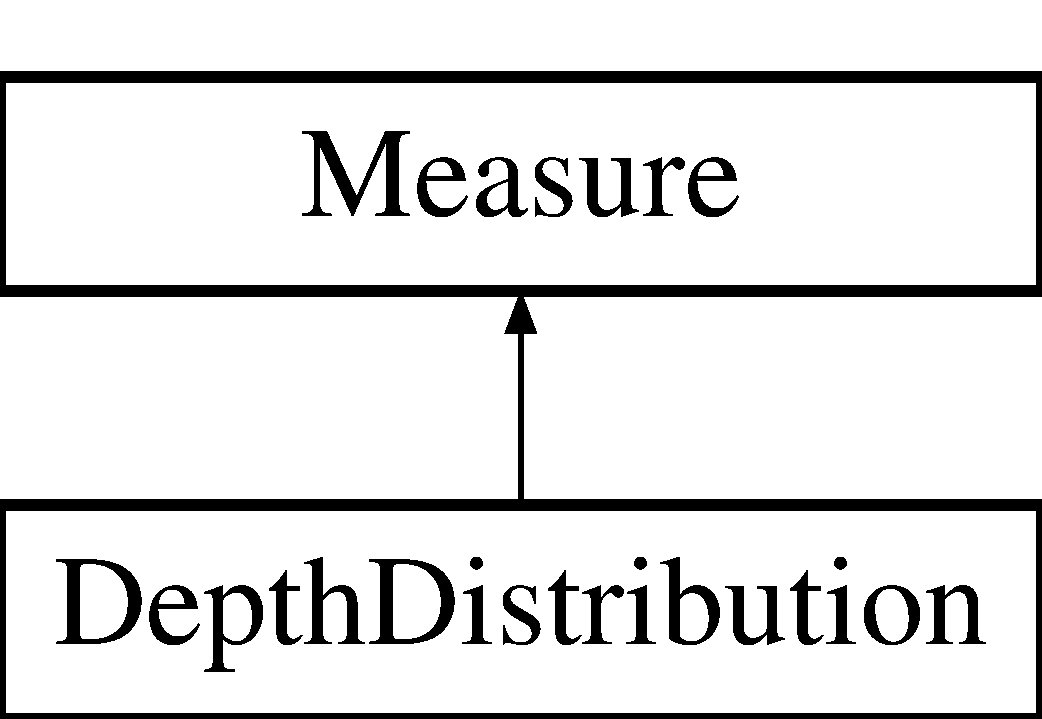
\includegraphics[height=2.000000cm]{class_depth_distribution}
\end{center}
\end{figure}
\subsection*{Public Member Functions}
\begin{DoxyCompactItemize}
\item 
\hyperlink{class_depth_distribution_a84d1d62eaad4b959aa61a3202e880d45}{Depth\+Distribution} (const Q\+String \&p\+Name)
\begin{DoxyCompactList}\small\item\em Constructor. \end{DoxyCompactList}\item 
\hyperlink{class_depth_distribution_a9f0042416af38e18a6fe0e7ab828103e}{$\sim$\+Depth\+Distribution} ()
\begin{DoxyCompactList}\small\item\em Destructor. \end{DoxyCompactList}\item 
void \hyperlink{class_depth_distribution_a2ae6d36e74346f0c6140d5e62f8b2e21}{Compute} (const \hyperlink{class_scene_information_builder}{Scene\+Information\+Builder} $\ast$p\+Scene\+Information\+Builder)
\begin{DoxyCompactList}\small\item\em Method that computes the measure. \end{DoxyCompactList}\end{DoxyCompactItemize}
\subsection*{Additional Inherited Members}


\subsection{Detailed Description}
Class that implements the depth distribution \mbox{[}Secord et al. 2011\mbox{]}. 

\begin{DoxyAuthor}{Author}
Xavier Bonaventura 

Copyright\+: (c) Universitat de Girona 
\end{DoxyAuthor}


\subsection{Constructor \& Destructor Documentation}
\hypertarget{class_depth_distribution_a84d1d62eaad4b959aa61a3202e880d45}{\index{Depth\+Distribution@{Depth\+Distribution}!Depth\+Distribution@{Depth\+Distribution}}
\index{Depth\+Distribution@{Depth\+Distribution}!Depth\+Distribution@{Depth\+Distribution}}
\subsubsection[{Depth\+Distribution}]{\setlength{\rightskip}{0pt plus 5cm}Depth\+Distribution\+::\+Depth\+Distribution (
\begin{DoxyParamCaption}
\item[{const Q\+String \&}]{p\+Name}
\end{DoxyParamCaption}
)}}\label{class_depth_distribution_a84d1d62eaad4b959aa61a3202e880d45}


Constructor. 

\hypertarget{class_depth_distribution_a9f0042416af38e18a6fe0e7ab828103e}{\index{Depth\+Distribution@{Depth\+Distribution}!````~Depth\+Distribution@{$\sim$\+Depth\+Distribution}}
\index{````~Depth\+Distribution@{$\sim$\+Depth\+Distribution}!Depth\+Distribution@{Depth\+Distribution}}
\subsubsection[{$\sim$\+Depth\+Distribution}]{\setlength{\rightskip}{0pt plus 5cm}Depth\+Distribution\+::$\sim$\+Depth\+Distribution (
\begin{DoxyParamCaption}
{}
\end{DoxyParamCaption}
)}}\label{class_depth_distribution_a9f0042416af38e18a6fe0e7ab828103e}


Destructor. 



\subsection{Member Function Documentation}
\hypertarget{class_depth_distribution_a2ae6d36e74346f0c6140d5e62f8b2e21}{\index{Depth\+Distribution@{Depth\+Distribution}!Compute@{Compute}}
\index{Compute@{Compute}!Depth\+Distribution@{Depth\+Distribution}}
\subsubsection[{Compute}]{\setlength{\rightskip}{0pt plus 5cm}void Depth\+Distribution\+::\+Compute (
\begin{DoxyParamCaption}
\item[{const {\bf Scene\+Information\+Builder} $\ast$}]{p\+Scene\+Information\+Builder}
\end{DoxyParamCaption}
)\hspace{0.3cm}{\ttfamily [virtual]}}}\label{class_depth_distribution_a2ae6d36e74346f0c6140d5e62f8b2e21}


Method that computes the measure. 



Implements \hyperlink{class_measure_aed88fe46b2a609ab5948e5f3c891321d}{Measure}.



The documentation for this class was generated from the following files\+:\begin{DoxyCompactItemize}
\item 
inc/viewpoint-\/measures/\hyperlink{_depth_distribution_8h}{Depth\+Distribution.\+h}\item 
src/viewpoint-\/measures/\hyperlink{_depth_distribution_8cpp}{Depth\+Distribution.\+cpp}\end{DoxyCompactItemize}

\hypertarget{class_dutagaci_dialog}{\section{Dutagaci\+Dialog Class Reference}
\label{class_dutagaci_dialog}\index{Dutagaci\+Dialog@{Dutagaci\+Dialog}}
}


Dialog to run the Dutagaci benchmark.  




{\ttfamily \#include $<$Dutagaci\+Dialog.\+h$>$}

Inheritance diagram for Dutagaci\+Dialog\+:\begin{figure}[H]
\begin{center}
\leavevmode
\includegraphics[height=2.000000cm]{class_dutagaci_dialog}
\end{center}
\end{figure}
\subsection*{Public Member Functions}
\begin{DoxyCompactItemize}
\item 
\hyperlink{class_dutagaci_dialog_a60ba64d79774ee46864dee12d8cd41cf}{Dutagaci\+Dialog} (Q\+Widget $\ast$parent=0)
\item 
\hyperlink{class_dutagaci_dialog_afc0b306a809090930a4646d2793b6eb3}{$\sim$\+Dutagaci\+Dialog} ()
\item 
Q\+Vector$<$ Q\+String $>$ \hyperlink{class_dutagaci_dialog_a133408f50e8890a5b7198790dfab153e}{Get\+Files\+To\+Load} () const 
\begin{DoxyCompactList}\small\item\em Return the list of files loaded in the dialog. \end{DoxyCompactList}\item 
float \hyperlink{class_dutagaci_dialog_a0ccfbc81cbfe1d47a1e0672981522df1}{Get\+Distance} () const 
\begin{DoxyCompactList}\small\item\em Get the distance as times the radius of the scene. \end{DoxyCompactList}\item 
int \hyperlink{class_dutagaci_dialog_afffe503535e80f9c2acaf9e47bff4d90}{Get\+Angle} () const 
\begin{DoxyCompactList}\small\item\em Get the field of view of the cameras. \end{DoxyCompactList}\end{DoxyCompactItemize}
\subsection*{Private Slots}
\begin{DoxyCompactItemize}
\item 
void \hyperlink{class_dutagaci_dialog_a5123e9a0c94d27945c7ce6f6c7f680b5}{on\+\_\+compute\+Camera\+Distance\+Button\+\_\+clicked} ()
\begin{DoxyCompactList}\small\item\em Compute camera distance button method. \end{DoxyCompactList}\item 
void \hyperlink{class_dutagaci_dialog_a6c7e1eedfc75bfe332e47e31877a07e7}{on\+\_\+compute\+Camera\+Angle\+Button\+\_\+clicked} ()
\begin{DoxyCompactList}\small\item\em Compute camera angle button method. \end{DoxyCompactList}\item 
void \hyperlink{class_dutagaci_dialog_a4fa0455f5f2ea033acc66db4c42b60f8}{on\+\_\+add\+Button\+\_\+clicked} ()
\begin{DoxyCompactList}\small\item\em Add button clicked method. \end{DoxyCompactList}\item 
void \hyperlink{class_dutagaci_dialog_a32f20e660a56aa8e789ce9c97b526bfc}{on\+\_\+delette\+Button\+\_\+clicked} ()
\begin{DoxyCompactList}\small\item\em Delete button clicked method. \end{DoxyCompactList}\item 
void \hyperlink{class_dutagaci_dialog_a87e953653f670bef399d7889bab618cd}{on\+\_\+compute\+Matrices\+Button\+\_\+clicked} ()
\begin{DoxyCompactList}\small\item\em Compute matrices button clicked method. \end{DoxyCompactList}\end{DoxyCompactItemize}
\subsection*{Private Member Functions}
\begin{DoxyCompactItemize}
\item 
Q\+Vector$<$ Q\+String $>$ \hyperlink{class_dutagaci_dialog_a6eace3feddf7a9e1bd39a1d0fa3e869e}{Get\+File\+List\+From\+T\+X\+T} (const Q\+String \&p\+File\+Name) const 
\end{DoxyCompactItemize}
\subsection*{Private Attributes}
\begin{DoxyCompactItemize}
\item 
Ui\+::\+Dutagaci\+View $\ast$ \hyperlink{class_dutagaci_dialog_a3ce0e7c4ba85b03b92859701b5f9cfc4}{m\+Ui}
\begin{DoxyCompactList}\small\item\em User interface. \end{DoxyCompactList}\item 
Q\+Vector$<$ Q\+String $>$ \hyperlink{class_dutagaci_dialog_a4a1130da190ed6fb4a941bb2236d219c}{m\+Files\+To\+Load}
\item 
float \hyperlink{class_dutagaci_dialog_a5aa43ab7213d5a88caad384c94141cbf}{m\+Distance}
\item 
int \hyperlink{class_dutagaci_dialog_acf6158ec2765efe1c6b8d4ef94eb14ff}{m\+Angle}
\end{DoxyCompactItemize}


\subsection{Detailed Description}
Dialog to run the Dutagaci benchmark. 

\begin{DoxyAuthor}{Author}
Xavier Bonaventura 

Copyright\+: (c) Universitat de Girona 
\end{DoxyAuthor}


\subsection{Constructor \& Destructor Documentation}
\hypertarget{class_dutagaci_dialog_a60ba64d79774ee46864dee12d8cd41cf}{\index{Dutagaci\+Dialog@{Dutagaci\+Dialog}!Dutagaci\+Dialog@{Dutagaci\+Dialog}}
\index{Dutagaci\+Dialog@{Dutagaci\+Dialog}!Dutagaci\+Dialog@{Dutagaci\+Dialog}}
\subsubsection[{Dutagaci\+Dialog}]{\setlength{\rightskip}{0pt plus 5cm}Dutagaci\+Dialog\+::\+Dutagaci\+Dialog (
\begin{DoxyParamCaption}
\item[{Q\+Widget $\ast$}]{parent = {\ttfamily 0}}
\end{DoxyParamCaption}
)\hspace{0.3cm}{\ttfamily [explicit]}}}\label{class_dutagaci_dialog_a60ba64d79774ee46864dee12d8cd41cf}
\hypertarget{class_dutagaci_dialog_afc0b306a809090930a4646d2793b6eb3}{\index{Dutagaci\+Dialog@{Dutagaci\+Dialog}!````~Dutagaci\+Dialog@{$\sim$\+Dutagaci\+Dialog}}
\index{````~Dutagaci\+Dialog@{$\sim$\+Dutagaci\+Dialog}!Dutagaci\+Dialog@{Dutagaci\+Dialog}}
\subsubsection[{$\sim$\+Dutagaci\+Dialog}]{\setlength{\rightskip}{0pt plus 5cm}Dutagaci\+Dialog\+::$\sim$\+Dutagaci\+Dialog (
\begin{DoxyParamCaption}
{}
\end{DoxyParamCaption}
)}}\label{class_dutagaci_dialog_afc0b306a809090930a4646d2793b6eb3}


\subsection{Member Function Documentation}
\hypertarget{class_dutagaci_dialog_afffe503535e80f9c2acaf9e47bff4d90}{\index{Dutagaci\+Dialog@{Dutagaci\+Dialog}!Get\+Angle@{Get\+Angle}}
\index{Get\+Angle@{Get\+Angle}!Dutagaci\+Dialog@{Dutagaci\+Dialog}}
\subsubsection[{Get\+Angle}]{\setlength{\rightskip}{0pt plus 5cm}int Dutagaci\+Dialog\+::\+Get\+Angle (
\begin{DoxyParamCaption}
{}
\end{DoxyParamCaption}
) const}}\label{class_dutagaci_dialog_afffe503535e80f9c2acaf9e47bff4d90}


Get the field of view of the cameras. 

\hypertarget{class_dutagaci_dialog_a0ccfbc81cbfe1d47a1e0672981522df1}{\index{Dutagaci\+Dialog@{Dutagaci\+Dialog}!Get\+Distance@{Get\+Distance}}
\index{Get\+Distance@{Get\+Distance}!Dutagaci\+Dialog@{Dutagaci\+Dialog}}
\subsubsection[{Get\+Distance}]{\setlength{\rightskip}{0pt plus 5cm}float Dutagaci\+Dialog\+::\+Get\+Distance (
\begin{DoxyParamCaption}
{}
\end{DoxyParamCaption}
) const}}\label{class_dutagaci_dialog_a0ccfbc81cbfe1d47a1e0672981522df1}


Get the distance as times the radius of the scene. 

\hypertarget{class_dutagaci_dialog_a6eace3feddf7a9e1bd39a1d0fa3e869e}{\index{Dutagaci\+Dialog@{Dutagaci\+Dialog}!Get\+File\+List\+From\+T\+X\+T@{Get\+File\+List\+From\+T\+X\+T}}
\index{Get\+File\+List\+From\+T\+X\+T@{Get\+File\+List\+From\+T\+X\+T}!Dutagaci\+Dialog@{Dutagaci\+Dialog}}
\subsubsection[{Get\+File\+List\+From\+T\+X\+T}]{\setlength{\rightskip}{0pt plus 5cm}Q\+Vector$<$ Q\+String $>$ Dutagaci\+Dialog\+::\+Get\+File\+List\+From\+T\+X\+T (
\begin{DoxyParamCaption}
\item[{const Q\+String \&}]{p\+File\+Name}
\end{DoxyParamCaption}
) const\hspace{0.3cm}{\ttfamily [private]}}}\label{class_dutagaci_dialog_a6eace3feddf7a9e1bd39a1d0fa3e869e}
\hypertarget{class_dutagaci_dialog_a133408f50e8890a5b7198790dfab153e}{\index{Dutagaci\+Dialog@{Dutagaci\+Dialog}!Get\+Files\+To\+Load@{Get\+Files\+To\+Load}}
\index{Get\+Files\+To\+Load@{Get\+Files\+To\+Load}!Dutagaci\+Dialog@{Dutagaci\+Dialog}}
\subsubsection[{Get\+Files\+To\+Load}]{\setlength{\rightskip}{0pt plus 5cm}Q\+Vector$<$ Q\+String $>$ Dutagaci\+Dialog\+::\+Get\+Files\+To\+Load (
\begin{DoxyParamCaption}
{}
\end{DoxyParamCaption}
) const}}\label{class_dutagaci_dialog_a133408f50e8890a5b7198790dfab153e}


Return the list of files loaded in the dialog. 

\hypertarget{class_dutagaci_dialog_a4fa0455f5f2ea033acc66db4c42b60f8}{\index{Dutagaci\+Dialog@{Dutagaci\+Dialog}!on\+\_\+add\+Button\+\_\+clicked@{on\+\_\+add\+Button\+\_\+clicked}}
\index{on\+\_\+add\+Button\+\_\+clicked@{on\+\_\+add\+Button\+\_\+clicked}!Dutagaci\+Dialog@{Dutagaci\+Dialog}}
\subsubsection[{on\+\_\+add\+Button\+\_\+clicked}]{\setlength{\rightskip}{0pt plus 5cm}void Dutagaci\+Dialog\+::on\+\_\+add\+Button\+\_\+clicked (
\begin{DoxyParamCaption}
{}
\end{DoxyParamCaption}
)\hspace{0.3cm}{\ttfamily [private]}, {\ttfamily [slot]}}}\label{class_dutagaci_dialog_a4fa0455f5f2ea033acc66db4c42b60f8}


Add button clicked method. 

\hypertarget{class_dutagaci_dialog_a6c7e1eedfc75bfe332e47e31877a07e7}{\index{Dutagaci\+Dialog@{Dutagaci\+Dialog}!on\+\_\+compute\+Camera\+Angle\+Button\+\_\+clicked@{on\+\_\+compute\+Camera\+Angle\+Button\+\_\+clicked}}
\index{on\+\_\+compute\+Camera\+Angle\+Button\+\_\+clicked@{on\+\_\+compute\+Camera\+Angle\+Button\+\_\+clicked}!Dutagaci\+Dialog@{Dutagaci\+Dialog}}
\subsubsection[{on\+\_\+compute\+Camera\+Angle\+Button\+\_\+clicked}]{\setlength{\rightskip}{0pt plus 5cm}void Dutagaci\+Dialog\+::on\+\_\+compute\+Camera\+Angle\+Button\+\_\+clicked (
\begin{DoxyParamCaption}
{}
\end{DoxyParamCaption}
)\hspace{0.3cm}{\ttfamily [private]}, {\ttfamily [slot]}}}\label{class_dutagaci_dialog_a6c7e1eedfc75bfe332e47e31877a07e7}


Compute camera angle button method. 

\hypertarget{class_dutagaci_dialog_a5123e9a0c94d27945c7ce6f6c7f680b5}{\index{Dutagaci\+Dialog@{Dutagaci\+Dialog}!on\+\_\+compute\+Camera\+Distance\+Button\+\_\+clicked@{on\+\_\+compute\+Camera\+Distance\+Button\+\_\+clicked}}
\index{on\+\_\+compute\+Camera\+Distance\+Button\+\_\+clicked@{on\+\_\+compute\+Camera\+Distance\+Button\+\_\+clicked}!Dutagaci\+Dialog@{Dutagaci\+Dialog}}
\subsubsection[{on\+\_\+compute\+Camera\+Distance\+Button\+\_\+clicked}]{\setlength{\rightskip}{0pt plus 5cm}void Dutagaci\+Dialog\+::on\+\_\+compute\+Camera\+Distance\+Button\+\_\+clicked (
\begin{DoxyParamCaption}
{}
\end{DoxyParamCaption}
)\hspace{0.3cm}{\ttfamily [private]}, {\ttfamily [slot]}}}\label{class_dutagaci_dialog_a5123e9a0c94d27945c7ce6f6c7f680b5}


Compute camera distance button method. 

\hypertarget{class_dutagaci_dialog_a87e953653f670bef399d7889bab618cd}{\index{Dutagaci\+Dialog@{Dutagaci\+Dialog}!on\+\_\+compute\+Matrices\+Button\+\_\+clicked@{on\+\_\+compute\+Matrices\+Button\+\_\+clicked}}
\index{on\+\_\+compute\+Matrices\+Button\+\_\+clicked@{on\+\_\+compute\+Matrices\+Button\+\_\+clicked}!Dutagaci\+Dialog@{Dutagaci\+Dialog}}
\subsubsection[{on\+\_\+compute\+Matrices\+Button\+\_\+clicked}]{\setlength{\rightskip}{0pt plus 5cm}void Dutagaci\+Dialog\+::on\+\_\+compute\+Matrices\+Button\+\_\+clicked (
\begin{DoxyParamCaption}
{}
\end{DoxyParamCaption}
)\hspace{0.3cm}{\ttfamily [private]}, {\ttfamily [slot]}}}\label{class_dutagaci_dialog_a87e953653f670bef399d7889bab618cd}


Compute matrices button clicked method. 

\hypertarget{class_dutagaci_dialog_a32f20e660a56aa8e789ce9c97b526bfc}{\index{Dutagaci\+Dialog@{Dutagaci\+Dialog}!on\+\_\+delette\+Button\+\_\+clicked@{on\+\_\+delette\+Button\+\_\+clicked}}
\index{on\+\_\+delette\+Button\+\_\+clicked@{on\+\_\+delette\+Button\+\_\+clicked}!Dutagaci\+Dialog@{Dutagaci\+Dialog}}
\subsubsection[{on\+\_\+delette\+Button\+\_\+clicked}]{\setlength{\rightskip}{0pt plus 5cm}void Dutagaci\+Dialog\+::on\+\_\+delette\+Button\+\_\+clicked (
\begin{DoxyParamCaption}
{}
\end{DoxyParamCaption}
)\hspace{0.3cm}{\ttfamily [private]}, {\ttfamily [slot]}}}\label{class_dutagaci_dialog_a32f20e660a56aa8e789ce9c97b526bfc}


Delete button clicked method. 



\subsection{Member Data Documentation}
\hypertarget{class_dutagaci_dialog_acf6158ec2765efe1c6b8d4ef94eb14ff}{\index{Dutagaci\+Dialog@{Dutagaci\+Dialog}!m\+Angle@{m\+Angle}}
\index{m\+Angle@{m\+Angle}!Dutagaci\+Dialog@{Dutagaci\+Dialog}}
\subsubsection[{m\+Angle}]{\setlength{\rightskip}{0pt plus 5cm}int Dutagaci\+Dialog\+::m\+Angle\hspace{0.3cm}{\ttfamily [private]}}}\label{class_dutagaci_dialog_acf6158ec2765efe1c6b8d4ef94eb14ff}
\hypertarget{class_dutagaci_dialog_a5aa43ab7213d5a88caad384c94141cbf}{\index{Dutagaci\+Dialog@{Dutagaci\+Dialog}!m\+Distance@{m\+Distance}}
\index{m\+Distance@{m\+Distance}!Dutagaci\+Dialog@{Dutagaci\+Dialog}}
\subsubsection[{m\+Distance}]{\setlength{\rightskip}{0pt plus 5cm}float Dutagaci\+Dialog\+::m\+Distance\hspace{0.3cm}{\ttfamily [private]}}}\label{class_dutagaci_dialog_a5aa43ab7213d5a88caad384c94141cbf}
\hypertarget{class_dutagaci_dialog_a4a1130da190ed6fb4a941bb2236d219c}{\index{Dutagaci\+Dialog@{Dutagaci\+Dialog}!m\+Files\+To\+Load@{m\+Files\+To\+Load}}
\index{m\+Files\+To\+Load@{m\+Files\+To\+Load}!Dutagaci\+Dialog@{Dutagaci\+Dialog}}
\subsubsection[{m\+Files\+To\+Load}]{\setlength{\rightskip}{0pt plus 5cm}Q\+Vector$<$Q\+String$>$ Dutagaci\+Dialog\+::m\+Files\+To\+Load\hspace{0.3cm}{\ttfamily [private]}}}\label{class_dutagaci_dialog_a4a1130da190ed6fb4a941bb2236d219c}
\hypertarget{class_dutagaci_dialog_a3ce0e7c4ba85b03b92859701b5f9cfc4}{\index{Dutagaci\+Dialog@{Dutagaci\+Dialog}!m\+Ui@{m\+Ui}}
\index{m\+Ui@{m\+Ui}!Dutagaci\+Dialog@{Dutagaci\+Dialog}}
\subsubsection[{m\+Ui}]{\setlength{\rightskip}{0pt plus 5cm}Ui\+::\+Dutagaci\+View$\ast$ Dutagaci\+Dialog\+::m\+Ui\hspace{0.3cm}{\ttfamily [private]}}}\label{class_dutagaci_dialog_a3ce0e7c4ba85b03b92859701b5f9cfc4}


User interface. 



The documentation for this class was generated from the following files\+:\begin{DoxyCompactItemize}
\item 
inc/\hyperlink{_dutagaci_dialog_8h}{Dutagaci\+Dialog.\+h}\item 
src/\hyperlink{_dutagaci_dialog_8cpp}{Dutagaci\+Dialog.\+cpp}\end{DoxyCompactItemize}

\hypertarget{class_feixas_saliency}{\section{Feixas\+Saliency Class Reference}
\label{class_feixas_saliency}\index{Feixas\+Saliency@{Feixas\+Saliency}}
}


Class that implements the saliency of a viewpoint \mbox{[}Feixas et al. 2009\mbox{]}.  




{\ttfamily \#include $<$Feixas\+Saliency.\+h$>$}

Inheritance diagram for Feixas\+Saliency\+:\begin{figure}[H]
\begin{center}
\leavevmode
\includegraphics[height=2.000000cm]{class_feixas_saliency}
\end{center}
\end{figure}
\subsection*{Public Member Functions}
\begin{DoxyCompactItemize}
\item 
\hyperlink{class_feixas_saliency_afbdd06af8664181c0ede69cacbabb5e4}{Feixas\+Saliency} (const Q\+String \&p\+Name)
\begin{DoxyCompactList}\small\item\em Constructor. \end{DoxyCompactList}\item 
\hyperlink{class_feixas_saliency_ad9ed1bf2aa1a7bca65916c2e20724e14}{$\sim$\+Feixas\+Saliency} ()
\begin{DoxyCompactList}\small\item\em Destructor. \end{DoxyCompactList}\item 
void \hyperlink{class_feixas_saliency_a86f01232be159669dc26b538c046b99c}{Compute} (const \hyperlink{class_scene_information_builder}{Scene\+Information\+Builder} $\ast$p\+Scene\+Information\+Builder)
\begin{DoxyCompactList}\small\item\em Method that computes the measure. \end{DoxyCompactList}\end{DoxyCompactItemize}
\subsection*{Private Member Functions}
\begin{DoxyCompactItemize}
\item 
float \hyperlink{class_feixas_saliency_a864ad3425a2544e74a139e48d58bac73}{Get\+Dissimilarity} (const \hyperlink{class_projected_areas_matrix}{Projected\+Areas\+Matrix} $\ast$p\+Projected\+Areas\+Matrix, int p\+Polygon\+I, int p\+Polygon\+J)
\begin{DoxyCompactList}\small\item\em Return the dissimilarity between two polygons. \end{DoxyCompactList}\end{DoxyCompactItemize}
\subsection*{Additional Inherited Members}


\subsection{Detailed Description}
Class that implements the saliency of a viewpoint \mbox{[}Feixas et al. 2009\mbox{]}. 

\begin{DoxyAuthor}{Author}
Xavier Bonaventura 

Copyright\+: (c) Universitat de Girona 
\end{DoxyAuthor}


\subsection{Constructor \& Destructor Documentation}
\hypertarget{class_feixas_saliency_afbdd06af8664181c0ede69cacbabb5e4}{\index{Feixas\+Saliency@{Feixas\+Saliency}!Feixas\+Saliency@{Feixas\+Saliency}}
\index{Feixas\+Saliency@{Feixas\+Saliency}!Feixas\+Saliency@{Feixas\+Saliency}}
\subsubsection[{Feixas\+Saliency}]{\setlength{\rightskip}{0pt plus 5cm}Feixas\+Saliency\+::\+Feixas\+Saliency (
\begin{DoxyParamCaption}
\item[{const Q\+String \&}]{p\+Name}
\end{DoxyParamCaption}
)}}\label{class_feixas_saliency_afbdd06af8664181c0ede69cacbabb5e4}


Constructor. 

\hypertarget{class_feixas_saliency_ad9ed1bf2aa1a7bca65916c2e20724e14}{\index{Feixas\+Saliency@{Feixas\+Saliency}!````~Feixas\+Saliency@{$\sim$\+Feixas\+Saliency}}
\index{````~Feixas\+Saliency@{$\sim$\+Feixas\+Saliency}!Feixas\+Saliency@{Feixas\+Saliency}}
\subsubsection[{$\sim$\+Feixas\+Saliency}]{\setlength{\rightskip}{0pt plus 5cm}Feixas\+Saliency\+::$\sim$\+Feixas\+Saliency (
\begin{DoxyParamCaption}
{}
\end{DoxyParamCaption}
)}}\label{class_feixas_saliency_ad9ed1bf2aa1a7bca65916c2e20724e14}


Destructor. 



\subsection{Member Function Documentation}
\hypertarget{class_feixas_saliency_a86f01232be159669dc26b538c046b99c}{\index{Feixas\+Saliency@{Feixas\+Saliency}!Compute@{Compute}}
\index{Compute@{Compute}!Feixas\+Saliency@{Feixas\+Saliency}}
\subsubsection[{Compute}]{\setlength{\rightskip}{0pt plus 5cm}void Feixas\+Saliency\+::\+Compute (
\begin{DoxyParamCaption}
\item[{const {\bf Scene\+Information\+Builder} $\ast$}]{p\+Scene\+Information\+Builder}
\end{DoxyParamCaption}
)\hspace{0.3cm}{\ttfamily [virtual]}}}\label{class_feixas_saliency_a86f01232be159669dc26b538c046b99c}


Method that computes the measure. 



Implements \hyperlink{class_measure_aed88fe46b2a609ab5948e5f3c891321d}{Measure}.

\hypertarget{class_feixas_saliency_a864ad3425a2544e74a139e48d58bac73}{\index{Feixas\+Saliency@{Feixas\+Saliency}!Get\+Dissimilarity@{Get\+Dissimilarity}}
\index{Get\+Dissimilarity@{Get\+Dissimilarity}!Feixas\+Saliency@{Feixas\+Saliency}}
\subsubsection[{Get\+Dissimilarity}]{\setlength{\rightskip}{0pt plus 5cm}float Feixas\+Saliency\+::\+Get\+Dissimilarity (
\begin{DoxyParamCaption}
\item[{const {\bf Projected\+Areas\+Matrix} $\ast$}]{p\+Projected\+Areas\+Matrix, }
\item[{int}]{p\+Polygon\+I, }
\item[{int}]{p\+Polygon\+J}
\end{DoxyParamCaption}
)\hspace{0.3cm}{\ttfamily [private]}}}\label{class_feixas_saliency_a864ad3425a2544e74a139e48d58bac73}


Return the dissimilarity between two polygons. 



The documentation for this class was generated from the following files\+:\begin{DoxyCompactItemize}
\item 
inc/viewpoint-\/measures/\hyperlink{_feixas_saliency_8h}{Feixas\+Saliency.\+h}\item 
src/viewpoint-\/measures/\hyperlink{_feixas_saliency_8cpp}{Feixas\+Saliency.\+cpp}\end{DoxyCompactItemize}

\hypertarget{class_geometry}{\section{Geometry Class Reference}
\label{class_geometry}\index{Geometry@{Geometry}}
}


Class to wrap the geometry of a 3d mesh that is not stored into the G\+P\+U until the Get\+G\+P\+U\+Geometry method is called.  




{\ttfamily \#include $<$Geometry.\+h$>$}

\subsection*{Public Types}
\begin{DoxyCompactItemize}
\item 
enum \hyperlink{class_geometry_af0136a3b268286ee5921cc6af5239293}{Topology} \{ \\*
\hyperlink{class_geometry_af0136a3b268286ee5921cc6af5239293a2dc58614ae2624eb5e9ef19ef0b2e3f7}{Points} = G\+L\+\_\+\+P\+O\+I\+N\+T\+S, 
\hyperlink{class_geometry_af0136a3b268286ee5921cc6af5239293a103668f674a21b448be2eb0ef0ee30df}{Lines} = G\+L\+\_\+\+L\+I\+N\+E\+S, 
\hyperlink{class_geometry_af0136a3b268286ee5921cc6af5239293a8f190b5e0cb67675c38b9eacfc609953}{Line\+\_\+\+Strip} = G\+L\+\_\+\+L\+I\+N\+E\+\_\+\+S\+T\+R\+I\+P, 
\hyperlink{class_geometry_af0136a3b268286ee5921cc6af5239293a1f5e0519d79112ee2ffe518e2f6371b6}{Line\+\_\+\+Loop} = G\+L\+\_\+\+L\+I\+N\+E\+\_\+\+L\+O\+O\+P, 
\\*
\hyperlink{class_geometry_af0136a3b268286ee5921cc6af5239293a892a36aa94ee995c59c11210ac98f088}{Triangles} = G\+L\+\_\+\+T\+R\+I\+A\+N\+G\+L\+E\+S
 \}
\begin{DoxyCompactList}\small\item\em Enumeration to define the topology of the geometry. \end{DoxyCompactList}\end{DoxyCompactItemize}
\subsection*{Public Member Functions}
\begin{DoxyCompactItemize}
\item 
\hyperlink{class_geometry_ae8f25281b573912b941d26a75ef5ce7b}{Geometry} (const Q\+String \&p\+Name, \hyperlink{class_geometry_af0136a3b268286ee5921cc6af5239293}{Topology} p\+T)
\begin{DoxyCompactList}\small\item\em Constructor. \end{DoxyCompactList}\item 
\hyperlink{class_geometry_add6d514eb5cc4e379432d92c6ae6c257}{Geometry} (const \hyperlink{class_geometry}{Geometry} \&p\+Geometry)
\begin{DoxyCompactList}\small\item\em Copy constructor (vertex neighbours have to be set again) \end{DoxyCompactList}\item 
\hyperlink{class_geometry_ad55e832122ab3a2833dcaa6507867678}{$\sim$\+Geometry} ()
\begin{DoxyCompactList}\small\item\em Destructor. \end{DoxyCompactList}\item 
void \hyperlink{class_geometry_a912818f30f8776abf60196f48b1a3415}{Set\+Vertices\+Data} (unsigned int p\+Size, const glm\+::vec4 $\ast$p\+Data)
\begin{DoxyCompactList}\small\item\em Set the vertices of the geometry. \end{DoxyCompactList}\item 
void \hyperlink{class_geometry_ae957bc46a1755764e31e58f22f0304a9}{Set\+Vertices\+Data} (unsigned int p\+Size, const glm\+::vec3 $\ast$p\+Data)
\begin{DoxyCompactList}\small\item\em Set the vertices of the geometry. \end{DoxyCompactList}\item 
void \hyperlink{class_geometry_add72fbd9292d479bb564d0b2521da7f9}{Set\+Vertices\+Data} (unsigned int p\+Size, const glm\+::vec2 $\ast$p\+Data)
\begin{DoxyCompactList}\small\item\em Set the vertices of the geometry. \end{DoxyCompactList}\item 
Q\+Vector$<$ float $>$ \hyperlink{class_geometry_a3eae5aa25ece2784ca0459a4f739f621}{Get\+Vertices\+Data} () const 
\begin{DoxyCompactList}\small\item\em Get the vertices of the geometry. \end{DoxyCompactList}\item 
unsigned int \hyperlink{class_geometry_a29977b97425c42535812af00262f1f91}{Get\+Vertex\+Stride} () const 
\begin{DoxyCompactList}\small\item\em Get vertex stride. \end{DoxyCompactList}\item 
void \hyperlink{class_geometry_a9296489a2f4a2d3046fa2db525e0c55f}{Set\+Normals\+Data} (unsigned int p\+Size, const glm\+::vec3 $\ast$p\+Data)
\begin{DoxyCompactList}\small\item\em Set the normals of the geometry. \end{DoxyCompactList}\item 
void \hyperlink{class_geometry_ac385bde3dd066a37a19898d724bf480b}{Set\+Color\+Data} (unsigned int p\+Size, const glm\+::vec4 $\ast$p\+Data)
\begin{DoxyCompactList}\small\item\em Set the colors of the geometry. \end{DoxyCompactList}\item 
void \hyperlink{class_geometry_ad3cc79f68c9ad93562ae7ea6d7b3acc0}{Set\+Color\+Data} (unsigned int p\+Size, const glm\+::vec3 $\ast$p\+Data)
\begin{DoxyCompactList}\small\item\em Set the colors of the geometry. \end{DoxyCompactList}\item 
void \hyperlink{class_geometry_a50937473645f0beb329bf116da9f442a}{Set\+Text\+Coords\+Data} (unsigned int p\+Size, const glm\+::vec2 $\ast$p\+Data)
\begin{DoxyCompactList}\small\item\em Set the texture coordinates of the geometry. \end{DoxyCompactList}\item 
void \hyperlink{class_geometry_a053c07a201e1519808ccdece2718bd95}{Set\+Tangent\+Data} (unsigned int p\+Size, const glm\+::vec3 $\ast$p\+Data)
\begin{DoxyCompactList}\small\item\em Set the tangents of the geometry. \end{DoxyCompactList}\item 
void \hyperlink{class_geometry_acbd0f21bbac3d33618dad636cce56503}{Set\+Bitangent\+Data} (unsigned int p\+Size, const glm\+::vec3 $\ast$p\+Data)
\begin{DoxyCompactList}\small\item\em Set the bitangents of the geometry. \end{DoxyCompactList}\item 
void \hyperlink{class_geometry_a1f303c21b32fca8f04d8adbcf23ecbbc}{Set\+Indexs\+Data} (unsigned int p\+Size, const unsigned int $\ast$p\+Data)
\begin{DoxyCompactList}\small\item\em Set the information of connectivities between vertices of the geometry. \end{DoxyCompactList}\item 
Q\+Vector$<$ unsigned int $>$ \hyperlink{class_geometry_a31440da8dc7f95faf6d02b04dc22b71b}{Get\+Indexs\+Data} () const 
\begin{DoxyCompactList}\small\item\em Get the information of connectivities between vertices of the geometry. \end{DoxyCompactList}\item 
void \hyperlink{class_geometry_a07481afac86ea0c4ae8193159533acde}{Set\+Name} (const Q\+String \&p\+Name)
\begin{DoxyCompactList}\small\item\em Set the name of the geometry. \end{DoxyCompactList}\item 
void \hyperlink{class_geometry_a6c406fec6e370cf1c9e3b3ea7c9f027b}{Set\+Topology} (\hyperlink{class_geometry_af0136a3b268286ee5921cc6af5239293}{Topology} p\+Topology)
\begin{DoxyCompactList}\small\item\em Set the topology. \end{DoxyCompactList}\item 
void \hyperlink{class_geometry_ac85092de7676b3f40d7a0bf4c75df8ba}{Compute\+Bounding\+Volumes} ()
\begin{DoxyCompactList}\small\item\em Compute the bounding volumes. \end{DoxyCompactList}\item 
void \hyperlink{class_geometry_ac5ca4e8358fd614fd15c1950a2b9d7e0}{Show\+Information} () const 
\begin{DoxyCompactList}\small\item\em Show information of the geometry like faces, vertices and diameter of the bounding sphere. \end{DoxyCompactList}\item 
\hyperlink{class_axis_aligned_bounding_box}{Axis\+Aligned\+Bounding\+Box} $\ast$ \hyperlink{class_geometry_a47a404fd7a0f65d0293b7133854d30c1}{Get\+Bounding\+Box} () const 
\begin{DoxyCompactList}\small\item\em Get the bounding box. \end{DoxyCompactList}\item 
const \hyperlink{class_bounding_sphere}{Bounding\+Sphere} $\ast$ \hyperlink{class_geometry_a9ca25aebc470b9f0866f53062a2468fc}{Get\+Bounding\+Sphere} () const 
\begin{DoxyCompactList}\small\item\em Get the bounding sphere. \end{DoxyCompactList}\item 
void \hyperlink{class_geometry_a164925c8b8713b573e3a50e54bff287a}{Draw} ()
\begin{DoxyCompactList}\small\item\em Draw the geometry. \end{DoxyCompactList}\item 
int \hyperlink{class_geometry_a72aa8f1408f2a037f9324d576b358afc}{Get\+Num\+Indices} () const 
\begin{DoxyCompactList}\small\item\em Get the number of indexes. \end{DoxyCompactList}\item 
int \hyperlink{class_geometry_a77ca9c5585d158cf69e4cd075ce3a81d}{Get\+Num\+Faces} () const 
\begin{DoxyCompactList}\small\item\em Get the number of faces. \end{DoxyCompactList}\item 
int \hyperlink{class_geometry_a69a4bb6e88c4c458602eb8a0fa1f13e7}{Get\+Num\+Vertices} () const 
\begin{DoxyCompactList}\small\item\em Get the number of vertices. \end{DoxyCompactList}\item 
\hyperlink{class_geometry_af0136a3b268286ee5921cc6af5239293}{Topology} \hyperlink{class_geometry_a2777696371d4cbc5a1a6b46bed273b96}{Get\+Topology} () const 
\begin{DoxyCompactList}\small\item\em Get the topology. \end{DoxyCompactList}\item 
const \hyperlink{class_g_p_u_geometry}{G\+P\+U\+Geometry} $\ast$ \hyperlink{class_geometry_a3b7103a7919fed0d1aafa3e4dc1c6cb2}{Get\+G\+P\+U\+Geometry} ()
\begin{DoxyCompactList}\small\item\em Get the \hyperlink{class_g_p_u_geometry}{G\+P\+U\+Geometry} creating it if it's necessary. \end{DoxyCompactList}\end{DoxyCompactItemize}
\subsection*{Private Attributes}
\begin{DoxyCompactItemize}
\item 
Q\+Vector$<$ float $>$ \hyperlink{class_geometry_aa1ab4726f4b285d37e98a69f212ac92a}{m\+Vertex\+Data}
\begin{DoxyCompactList}\small\item\em Data of the positions of the vertices. \end{DoxyCompactList}\item 
unsigned int \hyperlink{class_geometry_aa3d70589b74acec8de5487d1797204a6}{m\+Vertex\+Stride}
\begin{DoxyCompactList}\small\item\em Stride of the vertices. \end{DoxyCompactList}\item 
Q\+Vector$<$ float $>$ \hyperlink{class_geometry_aeb01f8834836e53482da4116bdcb7b42}{m\+Normal\+Data}
\begin{DoxyCompactList}\small\item\em Data of the normals of the vertices. \end{DoxyCompactList}\item 
Q\+Vector$<$ float $>$ \hyperlink{class_geometry_ad7e8ca05ff8a0629af98afedc5935b29}{m\+Color\+Data}
\begin{DoxyCompactList}\small\item\em Data of the colors of the vertices. \end{DoxyCompactList}\item 
unsigned int \hyperlink{class_geometry_afa6ac722cc0fad9071d5802560250eb3}{m\+Color\+Stride}
\begin{DoxyCompactList}\small\item\em Stride of the colors. \end{DoxyCompactList}\item 
Q\+Vector$<$ float $>$ \hyperlink{class_geometry_afd1dd852a551a6e2c4ea6fad41aceb68}{m\+Text\+Coords\+Data}
\begin{DoxyCompactList}\small\item\em Data of the texture coordinates of the vertices. \end{DoxyCompactList}\item 
Q\+Vector$<$ float $>$ \hyperlink{class_geometry_a7c1d990e17927df0bba609636ae646a2}{m\+Tangent\+Data}
\begin{DoxyCompactList}\small\item\em Data of the tangents of the vertices. \end{DoxyCompactList}\item 
Q\+Vector$<$ float $>$ \hyperlink{class_geometry_a965032c7634b3aaea165ffb1e9549b82}{m\+Bitangent\+Data}
\begin{DoxyCompactList}\small\item\em Data of the bitangents of the vertices. \end{DoxyCompactList}\item 
Q\+Vector$<$ unsigned int $>$ \hyperlink{class_geometry_ae0b8310174599d67910b0a5e33421106}{m\+Index\+Data}
\begin{DoxyCompactList}\small\item\em Data of the connectivity between vertices. \end{DoxyCompactList}\item 
Q\+String \hyperlink{class_geometry_a9831671d273039dd55c23be1198540eb}{m\+Name}
\begin{DoxyCompactList}\small\item\em Name of the geometry. \end{DoxyCompactList}\item 
\hyperlink{class_geometry_af0136a3b268286ee5921cc6af5239293}{Topology} \hyperlink{class_geometry_acfa146681080dedfb14420ba51b8b52a}{m\+Topology}
\begin{DoxyCompactList}\small\item\em Topology of the geometry. \end{DoxyCompactList}\item 
\hyperlink{class_axis_aligned_bounding_box}{Axis\+Aligned\+Bounding\+Box} $\ast$ \hyperlink{class_geometry_a8094cba464c4943a478092b73f7364f9}{m\+Bounding\+Box}
\begin{DoxyCompactList}\small\item\em Axis-\/aligned bounding box. \end{DoxyCompactList}\item 
\hyperlink{class_bounding_sphere}{Bounding\+Sphere} $\ast$ \hyperlink{class_geometry_a8dba41b46c1f6b4006a96449157b3357}{m\+Bounding\+Sphere}
\begin{DoxyCompactList}\small\item\em Bounding sphere. \end{DoxyCompactList}\item 
\hyperlink{class_g_p_u_geometry}{G\+P\+U\+Geometry} $\ast$ \hyperlink{class_geometry_a9df7e43cff221adde5c369d21a1933b9}{m\+G\+P\+U\+Geometry}
\begin{DoxyCompactList}\small\item\em G\+P\+U version of the geometry. \end{DoxyCompactList}\item 
bool \hyperlink{class_geometry_a44193e1c6e4d8678c0e466a1688a1d1b}{m\+Need\+G\+P\+U\+Geometry\+Update}
\begin{DoxyCompactList}\small\item\em Boolean to know if the \hyperlink{class_g_p_u_geometry}{G\+P\+U\+Geometry} needs to be updated. \end{DoxyCompactList}\end{DoxyCompactItemize}


\subsection{Detailed Description}
Class to wrap the geometry of a 3d mesh that is not stored into the G\+P\+U until the Get\+G\+P\+U\+Geometry method is called. 

\begin{DoxyAuthor}{Author}
Xavier Bonaventura 

Copyright\+: (c) Universitat de Girona 
\end{DoxyAuthor}


\subsection{Member Enumeration Documentation}
\hypertarget{class_geometry_af0136a3b268286ee5921cc6af5239293}{\index{Geometry@{Geometry}!Topology@{Topology}}
\index{Topology@{Topology}!Geometry@{Geometry}}
\subsubsection[{Topology}]{\setlength{\rightskip}{0pt plus 5cm}enum {\bf Geometry\+::\+Topology}}}\label{class_geometry_af0136a3b268286ee5921cc6af5239293}


Enumeration to define the topology of the geometry. 

\begin{Desc}
\item[Enumerator]\par
\begin{description}
\index{Points@{Points}!Geometry@{Geometry}}\index{Geometry@{Geometry}!Points@{Points}}\item[{\em 
\hypertarget{class_geometry_af0136a3b268286ee5921cc6af5239293a2dc58614ae2624eb5e9ef19ef0b2e3f7}{Points}\label{class_geometry_af0136a3b268286ee5921cc6af5239293a2dc58614ae2624eb5e9ef19ef0b2e3f7}
}]\index{Lines@{Lines}!Geometry@{Geometry}}\index{Geometry@{Geometry}!Lines@{Lines}}\item[{\em 
\hypertarget{class_geometry_af0136a3b268286ee5921cc6af5239293a103668f674a21b448be2eb0ef0ee30df}{Lines}\label{class_geometry_af0136a3b268286ee5921cc6af5239293a103668f674a21b448be2eb0ef0ee30df}
}]\index{Line\+\_\+\+Strip@{Line\+\_\+\+Strip}!Geometry@{Geometry}}\index{Geometry@{Geometry}!Line\+\_\+\+Strip@{Line\+\_\+\+Strip}}\item[{\em 
\hypertarget{class_geometry_af0136a3b268286ee5921cc6af5239293a8f190b5e0cb67675c38b9eacfc609953}{Line\+\_\+\+Strip}\label{class_geometry_af0136a3b268286ee5921cc6af5239293a8f190b5e0cb67675c38b9eacfc609953}
}]\index{Line\+\_\+\+Loop@{Line\+\_\+\+Loop}!Geometry@{Geometry}}\index{Geometry@{Geometry}!Line\+\_\+\+Loop@{Line\+\_\+\+Loop}}\item[{\em 
\hypertarget{class_geometry_af0136a3b268286ee5921cc6af5239293a1f5e0519d79112ee2ffe518e2f6371b6}{Line\+\_\+\+Loop}\label{class_geometry_af0136a3b268286ee5921cc6af5239293a1f5e0519d79112ee2ffe518e2f6371b6}
}]\index{Triangles@{Triangles}!Geometry@{Geometry}}\index{Geometry@{Geometry}!Triangles@{Triangles}}\item[{\em 
\hypertarget{class_geometry_af0136a3b268286ee5921cc6af5239293a892a36aa94ee995c59c11210ac98f088}{Triangles}\label{class_geometry_af0136a3b268286ee5921cc6af5239293a892a36aa94ee995c59c11210ac98f088}
}]\end{description}
\end{Desc}


\subsection{Constructor \& Destructor Documentation}
\hypertarget{class_geometry_ae8f25281b573912b941d26a75ef5ce7b}{\index{Geometry@{Geometry}!Geometry@{Geometry}}
\index{Geometry@{Geometry}!Geometry@{Geometry}}
\subsubsection[{Geometry}]{\setlength{\rightskip}{0pt plus 5cm}Geometry\+::\+Geometry (
\begin{DoxyParamCaption}
\item[{const Q\+String \&}]{p\+Name, }
\item[{{\bf Topology}}]{p\+T}
\end{DoxyParamCaption}
)}}\label{class_geometry_ae8f25281b573912b941d26a75ef5ce7b}


Constructor. 

\hypertarget{class_geometry_add6d514eb5cc4e379432d92c6ae6c257}{\index{Geometry@{Geometry}!Geometry@{Geometry}}
\index{Geometry@{Geometry}!Geometry@{Geometry}}
\subsubsection[{Geometry}]{\setlength{\rightskip}{0pt plus 5cm}Geometry\+::\+Geometry (
\begin{DoxyParamCaption}
\item[{const {\bf Geometry} \&}]{p\+Geometry}
\end{DoxyParamCaption}
)}}\label{class_geometry_add6d514eb5cc4e379432d92c6ae6c257}


Copy constructor (vertex neighbours have to be set again) 

\hypertarget{class_geometry_ad55e832122ab3a2833dcaa6507867678}{\index{Geometry@{Geometry}!````~Geometry@{$\sim$\+Geometry}}
\index{````~Geometry@{$\sim$\+Geometry}!Geometry@{Geometry}}
\subsubsection[{$\sim$\+Geometry}]{\setlength{\rightskip}{0pt plus 5cm}Geometry\+::$\sim$\+Geometry (
\begin{DoxyParamCaption}
{}
\end{DoxyParamCaption}
)}}\label{class_geometry_ad55e832122ab3a2833dcaa6507867678}


Destructor. 



\subsection{Member Function Documentation}
\hypertarget{class_geometry_ac85092de7676b3f40d7a0bf4c75df8ba}{\index{Geometry@{Geometry}!Compute\+Bounding\+Volumes@{Compute\+Bounding\+Volumes}}
\index{Compute\+Bounding\+Volumes@{Compute\+Bounding\+Volumes}!Geometry@{Geometry}}
\subsubsection[{Compute\+Bounding\+Volumes}]{\setlength{\rightskip}{0pt plus 5cm}void Geometry\+::\+Compute\+Bounding\+Volumes (
\begin{DoxyParamCaption}
{}
\end{DoxyParamCaption}
)}}\label{class_geometry_ac85092de7676b3f40d7a0bf4c75df8ba}


Compute the bounding volumes. 

\hypertarget{class_geometry_a164925c8b8713b573e3a50e54bff287a}{\index{Geometry@{Geometry}!Draw@{Draw}}
\index{Draw@{Draw}!Geometry@{Geometry}}
\subsubsection[{Draw}]{\setlength{\rightskip}{0pt plus 5cm}void Geometry\+::\+Draw (
\begin{DoxyParamCaption}
{}
\end{DoxyParamCaption}
)}}\label{class_geometry_a164925c8b8713b573e3a50e54bff287a}


Draw the geometry. 

\hypertarget{class_geometry_a47a404fd7a0f65d0293b7133854d30c1}{\index{Geometry@{Geometry}!Get\+Bounding\+Box@{Get\+Bounding\+Box}}
\index{Get\+Bounding\+Box@{Get\+Bounding\+Box}!Geometry@{Geometry}}
\subsubsection[{Get\+Bounding\+Box}]{\setlength{\rightskip}{0pt plus 5cm}{\bf Axis\+Aligned\+Bounding\+Box} $\ast$ Geometry\+::\+Get\+Bounding\+Box (
\begin{DoxyParamCaption}
{}
\end{DoxyParamCaption}
) const}}\label{class_geometry_a47a404fd7a0f65d0293b7133854d30c1}


Get the bounding box. 

\hypertarget{class_geometry_a9ca25aebc470b9f0866f53062a2468fc}{\index{Geometry@{Geometry}!Get\+Bounding\+Sphere@{Get\+Bounding\+Sphere}}
\index{Get\+Bounding\+Sphere@{Get\+Bounding\+Sphere}!Geometry@{Geometry}}
\subsubsection[{Get\+Bounding\+Sphere}]{\setlength{\rightskip}{0pt plus 5cm}const {\bf Bounding\+Sphere} $\ast$ Geometry\+::\+Get\+Bounding\+Sphere (
\begin{DoxyParamCaption}
{}
\end{DoxyParamCaption}
) const}}\label{class_geometry_a9ca25aebc470b9f0866f53062a2468fc}


Get the bounding sphere. 

\hypertarget{class_geometry_a3b7103a7919fed0d1aafa3e4dc1c6cb2}{\index{Geometry@{Geometry}!Get\+G\+P\+U\+Geometry@{Get\+G\+P\+U\+Geometry}}
\index{Get\+G\+P\+U\+Geometry@{Get\+G\+P\+U\+Geometry}!Geometry@{Geometry}}
\subsubsection[{Get\+G\+P\+U\+Geometry}]{\setlength{\rightskip}{0pt plus 5cm}const {\bf G\+P\+U\+Geometry} $\ast$ Geometry\+::\+Get\+G\+P\+U\+Geometry (
\begin{DoxyParamCaption}
{}
\end{DoxyParamCaption}
)}}\label{class_geometry_a3b7103a7919fed0d1aafa3e4dc1c6cb2}


Get the \hyperlink{class_g_p_u_geometry}{G\+P\+U\+Geometry} creating it if it's necessary. 

\hypertarget{class_geometry_a31440da8dc7f95faf6d02b04dc22b71b}{\index{Geometry@{Geometry}!Get\+Indexs\+Data@{Get\+Indexs\+Data}}
\index{Get\+Indexs\+Data@{Get\+Indexs\+Data}!Geometry@{Geometry}}
\subsubsection[{Get\+Indexs\+Data}]{\setlength{\rightskip}{0pt plus 5cm}Q\+Vector$<$ unsigned int $>$ Geometry\+::\+Get\+Indexs\+Data (
\begin{DoxyParamCaption}
{}
\end{DoxyParamCaption}
) const}}\label{class_geometry_a31440da8dc7f95faf6d02b04dc22b71b}


Get the information of connectivities between vertices of the geometry. 

\hypertarget{class_geometry_a77ca9c5585d158cf69e4cd075ce3a81d}{\index{Geometry@{Geometry}!Get\+Num\+Faces@{Get\+Num\+Faces}}
\index{Get\+Num\+Faces@{Get\+Num\+Faces}!Geometry@{Geometry}}
\subsubsection[{Get\+Num\+Faces}]{\setlength{\rightskip}{0pt plus 5cm}int Geometry\+::\+Get\+Num\+Faces (
\begin{DoxyParamCaption}
{}
\end{DoxyParamCaption}
) const}}\label{class_geometry_a77ca9c5585d158cf69e4cd075ce3a81d}


Get the number of faces. 

\hypertarget{class_geometry_a72aa8f1408f2a037f9324d576b358afc}{\index{Geometry@{Geometry}!Get\+Num\+Indices@{Get\+Num\+Indices}}
\index{Get\+Num\+Indices@{Get\+Num\+Indices}!Geometry@{Geometry}}
\subsubsection[{Get\+Num\+Indices}]{\setlength{\rightskip}{0pt plus 5cm}int Geometry\+::\+Get\+Num\+Indices (
\begin{DoxyParamCaption}
{}
\end{DoxyParamCaption}
) const}}\label{class_geometry_a72aa8f1408f2a037f9324d576b358afc}


Get the number of indexes. 

\hypertarget{class_geometry_a69a4bb6e88c4c458602eb8a0fa1f13e7}{\index{Geometry@{Geometry}!Get\+Num\+Vertices@{Get\+Num\+Vertices}}
\index{Get\+Num\+Vertices@{Get\+Num\+Vertices}!Geometry@{Geometry}}
\subsubsection[{Get\+Num\+Vertices}]{\setlength{\rightskip}{0pt plus 5cm}int Geometry\+::\+Get\+Num\+Vertices (
\begin{DoxyParamCaption}
{}
\end{DoxyParamCaption}
) const}}\label{class_geometry_a69a4bb6e88c4c458602eb8a0fa1f13e7}


Get the number of vertices. 

\hypertarget{class_geometry_a2777696371d4cbc5a1a6b46bed273b96}{\index{Geometry@{Geometry}!Get\+Topology@{Get\+Topology}}
\index{Get\+Topology@{Get\+Topology}!Geometry@{Geometry}}
\subsubsection[{Get\+Topology}]{\setlength{\rightskip}{0pt plus 5cm}{\bf Geometry\+::\+Topology} Geometry\+::\+Get\+Topology (
\begin{DoxyParamCaption}
{}
\end{DoxyParamCaption}
) const}}\label{class_geometry_a2777696371d4cbc5a1a6b46bed273b96}


Get the topology. 

\hypertarget{class_geometry_a29977b97425c42535812af00262f1f91}{\index{Geometry@{Geometry}!Get\+Vertex\+Stride@{Get\+Vertex\+Stride}}
\index{Get\+Vertex\+Stride@{Get\+Vertex\+Stride}!Geometry@{Geometry}}
\subsubsection[{Get\+Vertex\+Stride}]{\setlength{\rightskip}{0pt plus 5cm}unsigned int Geometry\+::\+Get\+Vertex\+Stride (
\begin{DoxyParamCaption}
{}
\end{DoxyParamCaption}
) const}}\label{class_geometry_a29977b97425c42535812af00262f1f91}


Get vertex stride. 

\hypertarget{class_geometry_a3eae5aa25ece2784ca0459a4f739f621}{\index{Geometry@{Geometry}!Get\+Vertices\+Data@{Get\+Vertices\+Data}}
\index{Get\+Vertices\+Data@{Get\+Vertices\+Data}!Geometry@{Geometry}}
\subsubsection[{Get\+Vertices\+Data}]{\setlength{\rightskip}{0pt plus 5cm}Q\+Vector$<$ float $>$ Geometry\+::\+Get\+Vertices\+Data (
\begin{DoxyParamCaption}
{}
\end{DoxyParamCaption}
) const}}\label{class_geometry_a3eae5aa25ece2784ca0459a4f739f621}


Get the vertices of the geometry. 

\hypertarget{class_geometry_acbd0f21bbac3d33618dad636cce56503}{\index{Geometry@{Geometry}!Set\+Bitangent\+Data@{Set\+Bitangent\+Data}}
\index{Set\+Bitangent\+Data@{Set\+Bitangent\+Data}!Geometry@{Geometry}}
\subsubsection[{Set\+Bitangent\+Data}]{\setlength{\rightskip}{0pt plus 5cm}void Geometry\+::\+Set\+Bitangent\+Data (
\begin{DoxyParamCaption}
\item[{unsigned int}]{p\+Size, }
\item[{const glm\+::vec3 $\ast$}]{p\+Data}
\end{DoxyParamCaption}
)}}\label{class_geometry_acbd0f21bbac3d33618dad636cce56503}


Set the bitangents of the geometry. 

\hypertarget{class_geometry_ac385bde3dd066a37a19898d724bf480b}{\index{Geometry@{Geometry}!Set\+Color\+Data@{Set\+Color\+Data}}
\index{Set\+Color\+Data@{Set\+Color\+Data}!Geometry@{Geometry}}
\subsubsection[{Set\+Color\+Data}]{\setlength{\rightskip}{0pt plus 5cm}void Geometry\+::\+Set\+Color\+Data (
\begin{DoxyParamCaption}
\item[{unsigned int}]{p\+Size, }
\item[{const glm\+::vec4 $\ast$}]{p\+Data}
\end{DoxyParamCaption}
)}}\label{class_geometry_ac385bde3dd066a37a19898d724bf480b}


Set the colors of the geometry. 

\hypertarget{class_geometry_ad3cc79f68c9ad93562ae7ea6d7b3acc0}{\index{Geometry@{Geometry}!Set\+Color\+Data@{Set\+Color\+Data}}
\index{Set\+Color\+Data@{Set\+Color\+Data}!Geometry@{Geometry}}
\subsubsection[{Set\+Color\+Data}]{\setlength{\rightskip}{0pt plus 5cm}void Geometry\+::\+Set\+Color\+Data (
\begin{DoxyParamCaption}
\item[{unsigned int}]{p\+Size, }
\item[{const glm\+::vec3 $\ast$}]{p\+Data}
\end{DoxyParamCaption}
)}}\label{class_geometry_ad3cc79f68c9ad93562ae7ea6d7b3acc0}


Set the colors of the geometry. 

\hypertarget{class_geometry_a1f303c21b32fca8f04d8adbcf23ecbbc}{\index{Geometry@{Geometry}!Set\+Indexs\+Data@{Set\+Indexs\+Data}}
\index{Set\+Indexs\+Data@{Set\+Indexs\+Data}!Geometry@{Geometry}}
\subsubsection[{Set\+Indexs\+Data}]{\setlength{\rightskip}{0pt plus 5cm}void Geometry\+::\+Set\+Indexs\+Data (
\begin{DoxyParamCaption}
\item[{unsigned int}]{p\+Size, }
\item[{const unsigned int $\ast$}]{p\+Data}
\end{DoxyParamCaption}
)}}\label{class_geometry_a1f303c21b32fca8f04d8adbcf23ecbbc}


Set the information of connectivities between vertices of the geometry. 

\hypertarget{class_geometry_a07481afac86ea0c4ae8193159533acde}{\index{Geometry@{Geometry}!Set\+Name@{Set\+Name}}
\index{Set\+Name@{Set\+Name}!Geometry@{Geometry}}
\subsubsection[{Set\+Name}]{\setlength{\rightskip}{0pt plus 5cm}void Geometry\+::\+Set\+Name (
\begin{DoxyParamCaption}
\item[{const Q\+String \&}]{p\+Name}
\end{DoxyParamCaption}
)}}\label{class_geometry_a07481afac86ea0c4ae8193159533acde}


Set the name of the geometry. 

\hypertarget{class_geometry_a9296489a2f4a2d3046fa2db525e0c55f}{\index{Geometry@{Geometry}!Set\+Normals\+Data@{Set\+Normals\+Data}}
\index{Set\+Normals\+Data@{Set\+Normals\+Data}!Geometry@{Geometry}}
\subsubsection[{Set\+Normals\+Data}]{\setlength{\rightskip}{0pt plus 5cm}void Geometry\+::\+Set\+Normals\+Data (
\begin{DoxyParamCaption}
\item[{unsigned int}]{p\+Size, }
\item[{const glm\+::vec3 $\ast$}]{p\+Data}
\end{DoxyParamCaption}
)}}\label{class_geometry_a9296489a2f4a2d3046fa2db525e0c55f}


Set the normals of the geometry. 

\hypertarget{class_geometry_a053c07a201e1519808ccdece2718bd95}{\index{Geometry@{Geometry}!Set\+Tangent\+Data@{Set\+Tangent\+Data}}
\index{Set\+Tangent\+Data@{Set\+Tangent\+Data}!Geometry@{Geometry}}
\subsubsection[{Set\+Tangent\+Data}]{\setlength{\rightskip}{0pt plus 5cm}void Geometry\+::\+Set\+Tangent\+Data (
\begin{DoxyParamCaption}
\item[{unsigned int}]{p\+Size, }
\item[{const glm\+::vec3 $\ast$}]{p\+Data}
\end{DoxyParamCaption}
)}}\label{class_geometry_a053c07a201e1519808ccdece2718bd95}


Set the tangents of the geometry. 

\hypertarget{class_geometry_a50937473645f0beb329bf116da9f442a}{\index{Geometry@{Geometry}!Set\+Text\+Coords\+Data@{Set\+Text\+Coords\+Data}}
\index{Set\+Text\+Coords\+Data@{Set\+Text\+Coords\+Data}!Geometry@{Geometry}}
\subsubsection[{Set\+Text\+Coords\+Data}]{\setlength{\rightskip}{0pt plus 5cm}void Geometry\+::\+Set\+Text\+Coords\+Data (
\begin{DoxyParamCaption}
\item[{unsigned int}]{p\+Size, }
\item[{const glm\+::vec2 $\ast$}]{p\+Data}
\end{DoxyParamCaption}
)}}\label{class_geometry_a50937473645f0beb329bf116da9f442a}


Set the texture coordinates of the geometry. 

\hypertarget{class_geometry_a6c406fec6e370cf1c9e3b3ea7c9f027b}{\index{Geometry@{Geometry}!Set\+Topology@{Set\+Topology}}
\index{Set\+Topology@{Set\+Topology}!Geometry@{Geometry}}
\subsubsection[{Set\+Topology}]{\setlength{\rightskip}{0pt plus 5cm}void Geometry\+::\+Set\+Topology (
\begin{DoxyParamCaption}
\item[{{\bf Topology}}]{p\+Topology}
\end{DoxyParamCaption}
)}}\label{class_geometry_a6c406fec6e370cf1c9e3b3ea7c9f027b}


Set the topology. 

\hypertarget{class_geometry_a912818f30f8776abf60196f48b1a3415}{\index{Geometry@{Geometry}!Set\+Vertices\+Data@{Set\+Vertices\+Data}}
\index{Set\+Vertices\+Data@{Set\+Vertices\+Data}!Geometry@{Geometry}}
\subsubsection[{Set\+Vertices\+Data}]{\setlength{\rightskip}{0pt plus 5cm}void Geometry\+::\+Set\+Vertices\+Data (
\begin{DoxyParamCaption}
\item[{unsigned int}]{p\+Size, }
\item[{const glm\+::vec4 $\ast$}]{p\+Data}
\end{DoxyParamCaption}
)}}\label{class_geometry_a912818f30f8776abf60196f48b1a3415}


Set the vertices of the geometry. 

\hypertarget{class_geometry_ae957bc46a1755764e31e58f22f0304a9}{\index{Geometry@{Geometry}!Set\+Vertices\+Data@{Set\+Vertices\+Data}}
\index{Set\+Vertices\+Data@{Set\+Vertices\+Data}!Geometry@{Geometry}}
\subsubsection[{Set\+Vertices\+Data}]{\setlength{\rightskip}{0pt plus 5cm}void Geometry\+::\+Set\+Vertices\+Data (
\begin{DoxyParamCaption}
\item[{unsigned int}]{p\+Size, }
\item[{const glm\+::vec3 $\ast$}]{p\+Data}
\end{DoxyParamCaption}
)}}\label{class_geometry_ae957bc46a1755764e31e58f22f0304a9}


Set the vertices of the geometry. 

\hypertarget{class_geometry_add72fbd9292d479bb564d0b2521da7f9}{\index{Geometry@{Geometry}!Set\+Vertices\+Data@{Set\+Vertices\+Data}}
\index{Set\+Vertices\+Data@{Set\+Vertices\+Data}!Geometry@{Geometry}}
\subsubsection[{Set\+Vertices\+Data}]{\setlength{\rightskip}{0pt plus 5cm}void Geometry\+::\+Set\+Vertices\+Data (
\begin{DoxyParamCaption}
\item[{unsigned int}]{p\+Size, }
\item[{const glm\+::vec2 $\ast$}]{p\+Data}
\end{DoxyParamCaption}
)}}\label{class_geometry_add72fbd9292d479bb564d0b2521da7f9}


Set the vertices of the geometry. 

\hypertarget{class_geometry_ac5ca4e8358fd614fd15c1950a2b9d7e0}{\index{Geometry@{Geometry}!Show\+Information@{Show\+Information}}
\index{Show\+Information@{Show\+Information}!Geometry@{Geometry}}
\subsubsection[{Show\+Information}]{\setlength{\rightskip}{0pt plus 5cm}void Geometry\+::\+Show\+Information (
\begin{DoxyParamCaption}
{}
\end{DoxyParamCaption}
) const}}\label{class_geometry_ac5ca4e8358fd614fd15c1950a2b9d7e0}


Show information of the geometry like faces, vertices and diameter of the bounding sphere. 



\subsection{Member Data Documentation}
\hypertarget{class_geometry_a965032c7634b3aaea165ffb1e9549b82}{\index{Geometry@{Geometry}!m\+Bitangent\+Data@{m\+Bitangent\+Data}}
\index{m\+Bitangent\+Data@{m\+Bitangent\+Data}!Geometry@{Geometry}}
\subsubsection[{m\+Bitangent\+Data}]{\setlength{\rightskip}{0pt plus 5cm}Q\+Vector$<$float$>$ Geometry\+::m\+Bitangent\+Data\hspace{0.3cm}{\ttfamily [private]}}}\label{class_geometry_a965032c7634b3aaea165ffb1e9549b82}


Data of the bitangents of the vertices. 

\hypertarget{class_geometry_a8094cba464c4943a478092b73f7364f9}{\index{Geometry@{Geometry}!m\+Bounding\+Box@{m\+Bounding\+Box}}
\index{m\+Bounding\+Box@{m\+Bounding\+Box}!Geometry@{Geometry}}
\subsubsection[{m\+Bounding\+Box}]{\setlength{\rightskip}{0pt plus 5cm}{\bf Axis\+Aligned\+Bounding\+Box}$\ast$ Geometry\+::m\+Bounding\+Box\hspace{0.3cm}{\ttfamily [private]}}}\label{class_geometry_a8094cba464c4943a478092b73f7364f9}


Axis-\/aligned bounding box. 

\hypertarget{class_geometry_a8dba41b46c1f6b4006a96449157b3357}{\index{Geometry@{Geometry}!m\+Bounding\+Sphere@{m\+Bounding\+Sphere}}
\index{m\+Bounding\+Sphere@{m\+Bounding\+Sphere}!Geometry@{Geometry}}
\subsubsection[{m\+Bounding\+Sphere}]{\setlength{\rightskip}{0pt plus 5cm}{\bf Bounding\+Sphere}$\ast$ Geometry\+::m\+Bounding\+Sphere\hspace{0.3cm}{\ttfamily [private]}}}\label{class_geometry_a8dba41b46c1f6b4006a96449157b3357}


Bounding sphere. 

\hypertarget{class_geometry_ad7e8ca05ff8a0629af98afedc5935b29}{\index{Geometry@{Geometry}!m\+Color\+Data@{m\+Color\+Data}}
\index{m\+Color\+Data@{m\+Color\+Data}!Geometry@{Geometry}}
\subsubsection[{m\+Color\+Data}]{\setlength{\rightskip}{0pt plus 5cm}Q\+Vector$<$float$>$ Geometry\+::m\+Color\+Data\hspace{0.3cm}{\ttfamily [private]}}}\label{class_geometry_ad7e8ca05ff8a0629af98afedc5935b29}


Data of the colors of the vertices. 

\hypertarget{class_geometry_afa6ac722cc0fad9071d5802560250eb3}{\index{Geometry@{Geometry}!m\+Color\+Stride@{m\+Color\+Stride}}
\index{m\+Color\+Stride@{m\+Color\+Stride}!Geometry@{Geometry}}
\subsubsection[{m\+Color\+Stride}]{\setlength{\rightskip}{0pt plus 5cm}unsigned int Geometry\+::m\+Color\+Stride\hspace{0.3cm}{\ttfamily [private]}}}\label{class_geometry_afa6ac722cc0fad9071d5802560250eb3}


Stride of the colors. 

\hypertarget{class_geometry_a9df7e43cff221adde5c369d21a1933b9}{\index{Geometry@{Geometry}!m\+G\+P\+U\+Geometry@{m\+G\+P\+U\+Geometry}}
\index{m\+G\+P\+U\+Geometry@{m\+G\+P\+U\+Geometry}!Geometry@{Geometry}}
\subsubsection[{m\+G\+P\+U\+Geometry}]{\setlength{\rightskip}{0pt plus 5cm}{\bf G\+P\+U\+Geometry}$\ast$ Geometry\+::m\+G\+P\+U\+Geometry\hspace{0.3cm}{\ttfamily [private]}}}\label{class_geometry_a9df7e43cff221adde5c369d21a1933b9}


G\+P\+U version of the geometry. 

\hypertarget{class_geometry_ae0b8310174599d67910b0a5e33421106}{\index{Geometry@{Geometry}!m\+Index\+Data@{m\+Index\+Data}}
\index{m\+Index\+Data@{m\+Index\+Data}!Geometry@{Geometry}}
\subsubsection[{m\+Index\+Data}]{\setlength{\rightskip}{0pt plus 5cm}Q\+Vector$<$unsigned int$>$ Geometry\+::m\+Index\+Data\hspace{0.3cm}{\ttfamily [private]}}}\label{class_geometry_ae0b8310174599d67910b0a5e33421106}


Data of the connectivity between vertices. 

\hypertarget{class_geometry_a9831671d273039dd55c23be1198540eb}{\index{Geometry@{Geometry}!m\+Name@{m\+Name}}
\index{m\+Name@{m\+Name}!Geometry@{Geometry}}
\subsubsection[{m\+Name}]{\setlength{\rightskip}{0pt plus 5cm}Q\+String Geometry\+::m\+Name\hspace{0.3cm}{\ttfamily [private]}}}\label{class_geometry_a9831671d273039dd55c23be1198540eb}


Name of the geometry. 

\hypertarget{class_geometry_a44193e1c6e4d8678c0e466a1688a1d1b}{\index{Geometry@{Geometry}!m\+Need\+G\+P\+U\+Geometry\+Update@{m\+Need\+G\+P\+U\+Geometry\+Update}}
\index{m\+Need\+G\+P\+U\+Geometry\+Update@{m\+Need\+G\+P\+U\+Geometry\+Update}!Geometry@{Geometry}}
\subsubsection[{m\+Need\+G\+P\+U\+Geometry\+Update}]{\setlength{\rightskip}{0pt plus 5cm}bool Geometry\+::m\+Need\+G\+P\+U\+Geometry\+Update\hspace{0.3cm}{\ttfamily [private]}}}\label{class_geometry_a44193e1c6e4d8678c0e466a1688a1d1b}


Boolean to know if the \hyperlink{class_g_p_u_geometry}{G\+P\+U\+Geometry} needs to be updated. 

\hypertarget{class_geometry_aeb01f8834836e53482da4116bdcb7b42}{\index{Geometry@{Geometry}!m\+Normal\+Data@{m\+Normal\+Data}}
\index{m\+Normal\+Data@{m\+Normal\+Data}!Geometry@{Geometry}}
\subsubsection[{m\+Normal\+Data}]{\setlength{\rightskip}{0pt plus 5cm}Q\+Vector$<$float$>$ Geometry\+::m\+Normal\+Data\hspace{0.3cm}{\ttfamily [private]}}}\label{class_geometry_aeb01f8834836e53482da4116bdcb7b42}


Data of the normals of the vertices. 

\hypertarget{class_geometry_a7c1d990e17927df0bba609636ae646a2}{\index{Geometry@{Geometry}!m\+Tangent\+Data@{m\+Tangent\+Data}}
\index{m\+Tangent\+Data@{m\+Tangent\+Data}!Geometry@{Geometry}}
\subsubsection[{m\+Tangent\+Data}]{\setlength{\rightskip}{0pt plus 5cm}Q\+Vector$<$float$>$ Geometry\+::m\+Tangent\+Data\hspace{0.3cm}{\ttfamily [private]}}}\label{class_geometry_a7c1d990e17927df0bba609636ae646a2}


Data of the tangents of the vertices. 

\hypertarget{class_geometry_afd1dd852a551a6e2c4ea6fad41aceb68}{\index{Geometry@{Geometry}!m\+Text\+Coords\+Data@{m\+Text\+Coords\+Data}}
\index{m\+Text\+Coords\+Data@{m\+Text\+Coords\+Data}!Geometry@{Geometry}}
\subsubsection[{m\+Text\+Coords\+Data}]{\setlength{\rightskip}{0pt plus 5cm}Q\+Vector$<$float$>$ Geometry\+::m\+Text\+Coords\+Data\hspace{0.3cm}{\ttfamily [private]}}}\label{class_geometry_afd1dd852a551a6e2c4ea6fad41aceb68}


Data of the texture coordinates of the vertices. 

\hypertarget{class_geometry_acfa146681080dedfb14420ba51b8b52a}{\index{Geometry@{Geometry}!m\+Topology@{m\+Topology}}
\index{m\+Topology@{m\+Topology}!Geometry@{Geometry}}
\subsubsection[{m\+Topology}]{\setlength{\rightskip}{0pt plus 5cm}{\bf Topology} Geometry\+::m\+Topology\hspace{0.3cm}{\ttfamily [private]}}}\label{class_geometry_acfa146681080dedfb14420ba51b8b52a}


Topology of the geometry. 

\hypertarget{class_geometry_aa1ab4726f4b285d37e98a69f212ac92a}{\index{Geometry@{Geometry}!m\+Vertex\+Data@{m\+Vertex\+Data}}
\index{m\+Vertex\+Data@{m\+Vertex\+Data}!Geometry@{Geometry}}
\subsubsection[{m\+Vertex\+Data}]{\setlength{\rightskip}{0pt plus 5cm}Q\+Vector$<$float$>$ Geometry\+::m\+Vertex\+Data\hspace{0.3cm}{\ttfamily [private]}}}\label{class_geometry_aa1ab4726f4b285d37e98a69f212ac92a}


Data of the positions of the vertices. 

\hypertarget{class_geometry_aa3d70589b74acec8de5487d1797204a6}{\index{Geometry@{Geometry}!m\+Vertex\+Stride@{m\+Vertex\+Stride}}
\index{m\+Vertex\+Stride@{m\+Vertex\+Stride}!Geometry@{Geometry}}
\subsubsection[{m\+Vertex\+Stride}]{\setlength{\rightskip}{0pt plus 5cm}unsigned int Geometry\+::m\+Vertex\+Stride\hspace{0.3cm}{\ttfamily [private]}}}\label{class_geometry_aa3d70589b74acec8de5487d1797204a6}


Stride of the vertices. 



The documentation for this class was generated from the following files\+:\begin{DoxyCompactItemize}
\item 
inc/core/\hyperlink{_geometry_8h}{Geometry.\+h}\item 
src/core/\hyperlink{_geometry_8cpp}{Geometry.\+cpp}\end{DoxyCompactItemize}

\hypertarget{class_gizmo}{\section{Gizmo Class Reference}
\label{class_gizmo}\index{Gizmo@{Gizmo}}
}


A gizmo is a special element that can be rendered but without any kind of illumination.  




{\ttfamily \#include $<$Gizmo.\+h$>$}

Inheritance diagram for Gizmo\+:\begin{figure}[H]
\begin{center}
\leavevmode
\includegraphics[height=2.608696cm]{class_gizmo}
\end{center}
\end{figure}
\subsection*{Public Member Functions}
\begin{DoxyCompactItemize}
\item 
\hyperlink{class_gizmo_a869c5618918e6a7d307017db4ced617f}{Gizmo} ()
\begin{DoxyCompactList}\small\item\em Constructor. \end{DoxyCompactList}\item 
\hyperlink{class_gizmo_a7ab775681e41082c52c11fa1eeb053ff}{Gizmo} (const \hyperlink{class_gizmo}{Gizmo} \&p\+Gizmo)
\begin{DoxyCompactList}\small\item\em Copy constructor. \end{DoxyCompactList}\item 
\hyperlink{class_gizmo_a308e8302907f2e51e05528f3473943a0}{$\sim$\+Gizmo} ()
\begin{DoxyCompactList}\small\item\em Destructor. \end{DoxyCompactList}\item 
void \hyperlink{class_gizmo_ab5ad6839e6387221d8f9ab3a17ba62f5}{Draw} ()
\begin{DoxyCompactList}\small\item\em Draw the gizmo. \end{DoxyCompactList}\item 
\hyperlink{class_geometry}{Geometry} $\ast$ \hyperlink{class_gizmo_a57b1c05ae3543998667896e4f967a022}{Get\+Mesh} () const 
\begin{DoxyCompactList}\small\item\em Get mesh. \end{DoxyCompactList}\end{DoxyCompactItemize}
\subsection*{Protected Member Functions}
\begin{DoxyCompactItemize}
\item 
virtual void \hyperlink{class_gizmo_a4ba36c75e6b8c2f729792de0161f5532}{Create\+Mesh} ()=0
\begin{DoxyCompactList}\small\item\em Create the mesh of the gizmo with the indexs, positions and colors. \end{DoxyCompactList}\item 
virtual void \hyperlink{class_gizmo_a30161525d80402eb0653f2612003a733}{Update\+Positions} ()=0
\begin{DoxyCompactList}\small\item\em Update the positions of the vertices of the mesh. \end{DoxyCompactList}\end{DoxyCompactItemize}
\subsection*{Protected Attributes}
\begin{DoxyCompactItemize}
\item 
\hyperlink{class_geometry}{Geometry} $\ast$ \hyperlink{class_gizmo_af458aa807ec26bd57dc3a58024dc5e5e}{m\+Gizmo}
\begin{DoxyCompactList}\small\item\em \hyperlink{class_mesh}{Mesh} that represents the gizmo. \end{DoxyCompactList}\item 
Q\+Vector$<$ glm\+::vec4 $>$ \hyperlink{class_gizmo_ae6e4173865120b76bf530f5f0ee8ec43}{m\+Position\+Of\+Vertices}
\begin{DoxyCompactList}\small\item\em Position of the vertices of the gizmo. \end{DoxyCompactList}\end{DoxyCompactItemize}


\subsection{Detailed Description}
A gizmo is a special element that can be rendered but without any kind of illumination. 

\begin{DoxyAuthor}{Author}
Xavier Bonaventura 

Copyright\+: (c) Universitat de Girona 
\end{DoxyAuthor}


\subsection{Constructor \& Destructor Documentation}
\hypertarget{class_gizmo_a869c5618918e6a7d307017db4ced617f}{\index{Gizmo@{Gizmo}!Gizmo@{Gizmo}}
\index{Gizmo@{Gizmo}!Gizmo@{Gizmo}}
\subsubsection[{Gizmo}]{\setlength{\rightskip}{0pt plus 5cm}Gizmo\+::\+Gizmo (
\begin{DoxyParamCaption}
{}
\end{DoxyParamCaption}
)}}\label{class_gizmo_a869c5618918e6a7d307017db4ced617f}


Constructor. 

\hypertarget{class_gizmo_a7ab775681e41082c52c11fa1eeb053ff}{\index{Gizmo@{Gizmo}!Gizmo@{Gizmo}}
\index{Gizmo@{Gizmo}!Gizmo@{Gizmo}}
\subsubsection[{Gizmo}]{\setlength{\rightskip}{0pt plus 5cm}Gizmo\+::\+Gizmo (
\begin{DoxyParamCaption}
\item[{const {\bf Gizmo} \&}]{p\+Gizmo}
\end{DoxyParamCaption}
)}}\label{class_gizmo_a7ab775681e41082c52c11fa1eeb053ff}


Copy constructor. 

\hypertarget{class_gizmo_a308e8302907f2e51e05528f3473943a0}{\index{Gizmo@{Gizmo}!````~Gizmo@{$\sim$\+Gizmo}}
\index{````~Gizmo@{$\sim$\+Gizmo}!Gizmo@{Gizmo}}
\subsubsection[{$\sim$\+Gizmo}]{\setlength{\rightskip}{0pt plus 5cm}Gizmo\+::$\sim$\+Gizmo (
\begin{DoxyParamCaption}
{}
\end{DoxyParamCaption}
)}}\label{class_gizmo_a308e8302907f2e51e05528f3473943a0}


Destructor. 



\subsection{Member Function Documentation}
\hypertarget{class_gizmo_a4ba36c75e6b8c2f729792de0161f5532}{\index{Gizmo@{Gizmo}!Create\+Mesh@{Create\+Mesh}}
\index{Create\+Mesh@{Create\+Mesh}!Gizmo@{Gizmo}}
\subsubsection[{Create\+Mesh}]{\setlength{\rightskip}{0pt plus 5cm}virtual void Gizmo\+::\+Create\+Mesh (
\begin{DoxyParamCaption}
{}
\end{DoxyParamCaption}
)\hspace{0.3cm}{\ttfamily [protected]}, {\ttfamily [pure virtual]}}}\label{class_gizmo_a4ba36c75e6b8c2f729792de0161f5532}


Create the mesh of the gizmo with the indexs, positions and colors. 



Implemented in \hyperlink{class_orthographic_camera_a5edb0b3f645e77d086024157ef684eea}{Orthographic\+Camera}, \hyperlink{class_axis_aligned_bounding_box_a4f6fdbced63eabf9e7f32632f20bb610}{Axis\+Aligned\+Bounding\+Box}, \hyperlink{class_bounding_sphere_a8bed6b6f60b7676d09c45b41db2032e6}{Bounding\+Sphere}, and \hyperlink{class_perspective_camera_acefab56b5bf9449e1a97e0f193702d36}{Perspective\+Camera}.

\hypertarget{class_gizmo_ab5ad6839e6387221d8f9ab3a17ba62f5}{\index{Gizmo@{Gizmo}!Draw@{Draw}}
\index{Draw@{Draw}!Gizmo@{Gizmo}}
\subsubsection[{Draw}]{\setlength{\rightskip}{0pt plus 5cm}void Gizmo\+::\+Draw (
\begin{DoxyParamCaption}
{}
\end{DoxyParamCaption}
)}}\label{class_gizmo_ab5ad6839e6387221d8f9ab3a17ba62f5}


Draw the gizmo. 

\hypertarget{class_gizmo_a57b1c05ae3543998667896e4f967a022}{\index{Gizmo@{Gizmo}!Get\+Mesh@{Get\+Mesh}}
\index{Get\+Mesh@{Get\+Mesh}!Gizmo@{Gizmo}}
\subsubsection[{Get\+Mesh}]{\setlength{\rightskip}{0pt plus 5cm}{\bf Geometry} $\ast$ Gizmo\+::\+Get\+Mesh (
\begin{DoxyParamCaption}
{}
\end{DoxyParamCaption}
) const}}\label{class_gizmo_a57b1c05ae3543998667896e4f967a022}


Get mesh. 

\hypertarget{class_gizmo_a30161525d80402eb0653f2612003a733}{\index{Gizmo@{Gizmo}!Update\+Positions@{Update\+Positions}}
\index{Update\+Positions@{Update\+Positions}!Gizmo@{Gizmo}}
\subsubsection[{Update\+Positions}]{\setlength{\rightskip}{0pt plus 5cm}virtual void Gizmo\+::\+Update\+Positions (
\begin{DoxyParamCaption}
{}
\end{DoxyParamCaption}
)\hspace{0.3cm}{\ttfamily [protected]}, {\ttfamily [pure virtual]}}}\label{class_gizmo_a30161525d80402eb0653f2612003a733}


Update the positions of the vertices of the mesh. 



Implemented in \hyperlink{class_orthographic_camera_ad774f1e383f99a94e3f733ecaa814e80}{Orthographic\+Camera}, \hyperlink{class_axis_aligned_bounding_box_a9682fe904e3c0c1369b4e94002c9b025}{Axis\+Aligned\+Bounding\+Box}, \hyperlink{class_bounding_sphere_ab1d394277a8f79bc970765af75273319}{Bounding\+Sphere}, and \hyperlink{class_perspective_camera_a80ca50f210c1ea07f346bcee9dff6451}{Perspective\+Camera}.



\subsection{Member Data Documentation}
\hypertarget{class_gizmo_af458aa807ec26bd57dc3a58024dc5e5e}{\index{Gizmo@{Gizmo}!m\+Gizmo@{m\+Gizmo}}
\index{m\+Gizmo@{m\+Gizmo}!Gizmo@{Gizmo}}
\subsubsection[{m\+Gizmo}]{\setlength{\rightskip}{0pt plus 5cm}{\bf Geometry}$\ast$ Gizmo\+::m\+Gizmo\hspace{0.3cm}{\ttfamily [protected]}}}\label{class_gizmo_af458aa807ec26bd57dc3a58024dc5e5e}


\hyperlink{class_mesh}{Mesh} that represents the gizmo. 

\hypertarget{class_gizmo_ae6e4173865120b76bf530f5f0ee8ec43}{\index{Gizmo@{Gizmo}!m\+Position\+Of\+Vertices@{m\+Position\+Of\+Vertices}}
\index{m\+Position\+Of\+Vertices@{m\+Position\+Of\+Vertices}!Gizmo@{Gizmo}}
\subsubsection[{m\+Position\+Of\+Vertices}]{\setlength{\rightskip}{0pt plus 5cm}Q\+Vector$<$glm\+::vec4$>$ Gizmo\+::m\+Position\+Of\+Vertices\hspace{0.3cm}{\ttfamily [protected]}}}\label{class_gizmo_ae6e4173865120b76bf530f5f0ee8ec43}


Position of the vertices of the gizmo. 



The documentation for this class was generated from the following files\+:\begin{DoxyCompactItemize}
\item 
inc/core/\hyperlink{_gizmo_8h}{Gizmo.\+h}\item 
src/core/\hyperlink{_gizmo_8cpp}{Gizmo.\+cpp}\end{DoxyCompactItemize}

\hypertarget{class_g_l_canvas}{\section{G\+L\+Canvas Class Reference}
\label{class_g_l_canvas}\index{G\+L\+Canvas@{G\+L\+Canvas}}
}


Class to do the Open\+G\+L render.  




{\ttfamily \#include $<$G\+L\+Canvas.\+h$>$}

Inheritance diagram for G\+L\+Canvas\+:\begin{figure}[H]
\begin{center}
\leavevmode
\includegraphics[height=2.000000cm]{class_g_l_canvas}
\end{center}
\end{figure}
\subsection*{Public Slots}
\begin{DoxyCompactItemize}
\item 
void \hyperlink{class_g_l_canvas_a037f909d5c50fc0503a46a9493184f56}{Will\+Draw\+Bounding\+Box} (bool p\+Draw)
\begin{DoxyCompactList}\small\item\em Set if the bounding boxes will be drawn. \end{DoxyCompactList}\item 
void \hyperlink{class_g_l_canvas_a2d8d63019be91a9146e9e9251f6933b9}{Will\+Draw\+Bounding\+Sphere} (bool p\+Draw)
\begin{DoxyCompactList}\small\item\em Set if the bounding spheres will be drawn. \end{DoxyCompactList}\item 
void \hyperlink{class_g_l_canvas_a37bc7b32309c45bbe36cb6813c5ccd95}{Apply\+Materials} (bool p\+Apply\+Materials)
\begin{DoxyCompactList}\small\item\em Set if the materials will be applied for the rendering. \end{DoxyCompactList}\end{DoxyCompactItemize}
\subsection*{Public Member Functions}
\begin{DoxyCompactItemize}
\item 
\hyperlink{class_g_l_canvas_a990c03d907317cf7c779c732879a5e09}{G\+L\+Canvas} (Q\+Widget $\ast$p\+Parent=0)
\begin{DoxyCompactList}\small\item\em Constructor. \end{DoxyCompactList}\item 
\hyperlink{class_g_l_canvas_ae0a190f77989c1ada0a2c18e014fe793}{$\sim$\+G\+L\+Canvas} ()
\begin{DoxyCompactList}\small\item\em Destructor. \end{DoxyCompactList}\item 
void \hyperlink{class_g_l_canvas_a4f0ed55a666acb49e62614ac852dbbd6}{Load\+Scene} (\hyperlink{class_scene}{Scene} $\ast$p\+Scene, const \hyperlink{class_camera}{Camera} $\ast$p\+Camera=N\+U\+L\+L)
\begin{DoxyCompactList}\small\item\em Load an scene. \end{DoxyCompactList}\item 
void \hyperlink{class_g_l_canvas_ad971519caad475d6e808a643a9cafa9e}{Set\+Per\+Vertex\+Mesh} (\hyperlink{class_geometry}{Geometry} $\ast$p\+Per\+Vertex\+Mesh)
\begin{DoxyCompactList}\small\item\em Initialize the list of meshes that will be render with the color per vertex with the parameter. \end{DoxyCompactList}\item 
void \hyperlink{class_g_l_canvas_a2d000cfd65bf699e1c518ad429cc5e1d}{Add\+Per\+Vertex\+Mesh} (\hyperlink{class_geometry}{Geometry} $\ast$p\+Per\+Vertex\+Mesh)
\begin{DoxyCompactList}\small\item\em Add a mesh that will be render with the color per vertex. \end{DoxyCompactList}\item 
\hyperlink{class_g_l_s_l_program}{G\+L\+S\+L\+Program} $\ast$ \hyperlink{class_g_l_canvas_a1c704fb20881551f24af638a12eebcdb}{Get\+Shader\+Program} () const 
\begin{DoxyCompactList}\small\item\em Get the program used to do the rendering. \end{DoxyCompactList}\item 
Q\+String \hyperlink{class_g_l_canvas_a16125e392094d96ff68452095e9a358e}{Save\+Screenshot} (const Q\+String \&p\+File\+Name)
\begin{DoxyCompactList}\small\item\em Save a screenshot of the renderer. \end{DoxyCompactList}\item 
void \hyperlink{class_g_l_canvas_a5dc3c27442c7bbcdeeb649888f39f6ea}{Set\+Camera} (const \hyperlink{class_camera}{Camera} $\ast$p\+Camera)
\begin{DoxyCompactList}\small\item\em Set the camera used to render. \end{DoxyCompactList}\item 
\hyperlink{class_camera}{Camera} $\ast$ \hyperlink{class_g_l_canvas_a580935482356ce4b627b51180bfb1c6b}{Get\+Camera} ()
\begin{DoxyCompactList}\small\item\em Get the camera used to render. \end{DoxyCompactList}\item 
\hyperlink{class_scene}{Scene} $\ast$ \hyperlink{class_g_l_canvas_a63cd5238d1da2877877abfe946138dde}{Get\+Scene} ()
\begin{DoxyCompactList}\small\item\em Get the scene rendered. \end{DoxyCompactList}\end{DoxyCompactItemize}
\subsection*{Protected Member Functions}
\begin{DoxyCompactItemize}
\item 
void \hyperlink{class_g_l_canvas_af2d9b9abb7f03f024e91d7357e3ba02a}{initialize\+G\+L} ()
\begin{DoxyCompactList}\small\item\em Initialize the Open\+G\+L. \end{DoxyCompactList}\item 
void \hyperlink{class_g_l_canvas_a8e33d257b75968f5e0ec4e458df9407b}{paint\+G\+L} ()
\begin{DoxyCompactList}\small\item\em Open\+G\+L paint method. \end{DoxyCompactList}\item 
void \hyperlink{class_g_l_canvas_aa329a08cd23838dd8c077b359ca537b2}{resize\+G\+L} (int p\+Width, int p\+Height)
\begin{DoxyCompactList}\small\item\em Method to catch the resize event. \end{DoxyCompactList}\item 
void \hyperlink{class_g_l_canvas_af5033d668a7e0ba6cce270351c1ed1f6}{key\+Press\+Event} (Q\+Key\+Event $\ast$p\+Event)
\begin{DoxyCompactList}\small\item\em Method to catch the key events. \end{DoxyCompactList}\end{DoxyCompactItemize}
\subsection*{Private Member Functions}
\begin{DoxyCompactItemize}
\item 
void \hyperlink{class_g_l_canvas_a674f6e5dc712d591efd37d9ee927a853}{Draw\+Geometry\+Bounding\+Volumes} ()
\begin{DoxyCompactList}\small\item\em Draw the bounding volumes. \end{DoxyCompactList}\item 
void \hyperlink{class_g_l_canvas_a8e5d4350658d48aa89dc6945387cb0e0}{Recompute\+Viewport} ()
\begin{DoxyCompactList}\small\item\em Recompute the viewport. \end{DoxyCompactList}\item 
void \hyperlink{class_g_l_canvas_a9b521effcd5bfb684f6bab80d284a4e4}{Load\+Shaders} ()
\begin{DoxyCompactList}\small\item\em Load the shaders. \end{DoxyCompactList}\item 
void \hyperlink{class_g_l_canvas_a342975ca2a4b968892ad212c5753f87e}{Delete\+Shaders} ()
\begin{DoxyCompactList}\small\item\em Delete the shaders. \end{DoxyCompactList}\item 
void \hyperlink{class_g_l_canvas_ab9f6c69aea4a15d1caff11e00c113e3f}{Init\+Dual\+Peeling\+Render\+Targets} ()
\begin{DoxyCompactList}\small\item\em Initialize the dual depth peeling render targets. \end{DoxyCompactList}\item 
void \hyperlink{class_g_l_canvas_ab4a82d05c1ccbc2a76d95318ce3d2cef}{Delete\+Dual\+Peeling\+Render\+Targets} ()
\begin{DoxyCompactList}\small\item\em Delete the dual depth peeling render targets. \end{DoxyCompactList}\end{DoxyCompactItemize}
\subsection*{Private Attributes}
\begin{DoxyCompactItemize}
\item 
bool \hyperlink{class_g_l_canvas_a29134dbb47d2929ec22466af3ff82fc6}{m\+Draw\+Bounding\+Box}
\begin{DoxyCompactList}\small\item\em Boolean to know if the bounding boxes will be drawn. \end{DoxyCompactList}\item 
bool \hyperlink{class_g_l_canvas_a8c5d1ccfff6a1d1d3d578b1f20414292}{m\+Draw\+Bounding\+Sphere}
\begin{DoxyCompactList}\small\item\em Boolean to know if the bounding spheres will be drawn. \end{DoxyCompactList}\item 
bool \hyperlink{class_g_l_canvas_adb8c8071a5e78417ff56355466992ca1}{m\+Draw\+Wireframe}
\begin{DoxyCompactList}\small\item\em Boolean to know if the sphere of viewpoints will be drawn in wireframe mode. \end{DoxyCompactList}\item 
bool \hyperlink{class_g_l_canvas_afee59d3997ff8cb4e05fb5a1244d5278}{m\+Apply\+Materials}
\begin{DoxyCompactList}\small\item\em Boolean to know if the materials will be applied for the rendering. \end{DoxyCompactList}\item 
\hyperlink{class_camera}{Camera} $\ast$ \hyperlink{class_g_l_canvas_a819693fdcfb9caccfa7b368edc3613c6}{m\+Free\+Camera}
\begin{DoxyCompactList}\small\item\em \hyperlink{class_camera}{Camera} used for the rendering. \end{DoxyCompactList}\item 
\hyperlink{class_scene}{Scene} $\ast$ \hyperlink{class_g_l_canvas_ad14c80647484e0ab65732ba971ed7b84}{m\+Scene}
\begin{DoxyCompactList}\small\item\em \hyperlink{class_scene}{Scene}. \end{DoxyCompactList}\item 
\hyperlink{class_g_p_u_scene}{G\+P\+U\+Scene} $\ast$ \hyperlink{class_g_l_canvas_a46e82ba1b95d09cbcb42e2db24c4d10a}{m\+G\+P\+U\+Scene}
\begin{DoxyCompactList}\small\item\em \hyperlink{class_scene}{Scene} that will be used for the rendering. \end{DoxyCompactList}\item 
Q\+Vector$<$ \hyperlink{class_geometry}{Geometry} $\ast$ $>$ \hyperlink{class_g_l_canvas_a7c28ed5eaacb35dddc0f8777e6b291ed}{m\+Per\+Vertex\+Color\+Meshes}
\begin{DoxyCompactList}\small\item\em Meshes that will be rendered by per vertex color. \end{DoxyCompactList}\item 
\hyperlink{class_g_l_s_l_program}{G\+L\+S\+L\+Program} $\ast$ \hyperlink{class_g_l_canvas_adad92626cf28f8115762dc7f1b6ddc04}{m\+Shader\+Dual\+Init}
\begin{DoxyCompactList}\small\item\em Shader used to initialize the min-\/max depth buffer for the dual depth peeling. \end{DoxyCompactList}\item 
\hyperlink{class_g_l_s_l_program}{G\+L\+S\+L\+Program} $\ast$ \hyperlink{class_g_l_canvas_a4321e3211f585a47a026f46de456267b}{m\+Shader\+Dual\+Peel}
\begin{DoxyCompactList}\small\item\em Shader used to do the main pass of the renderer. \end{DoxyCompactList}\item 
\hyperlink{class_g_l_s_l_program}{G\+L\+S\+L\+Program} $\ast$ \hyperlink{class_g_l_canvas_a78abb793d487793faf1e4870894264ee}{m\+Shader\+Dual\+Peel\+Per\+Vertex\+Color}
\begin{DoxyCompactList}\small\item\em Shader used to do the main pass of the renderer for the gizmos. \end{DoxyCompactList}\item 
\hyperlink{class_g_l_s_l_program}{G\+L\+S\+L\+Program} $\ast$ \hyperlink{class_g_l_canvas_a63597026b7698a27ca2b65947b07a8c4}{m\+Shader\+Dual\+Blend}
\begin{DoxyCompactList}\small\item\em Shader used to alpha-\/blend the back color for the dual depth peeling. \end{DoxyCompactList}\item 
\hyperlink{class_g_l_s_l_program}{G\+L\+S\+L\+Program} $\ast$ \hyperlink{class_g_l_canvas_a3da4afa0d1f292dddd869dffc7b5e5ec}{m\+Shader\+Dual\+Final}
\begin{DoxyCompactList}\small\item\em Shader used to combinte the color of the front and the back buffer for the dual depth peeling. \end{DoxyCompactList}\item 
G\+Luint \hyperlink{class_g_l_canvas_aadd45b922f81b641e051b497c15c6c24}{m\+Query\+Id}
\begin{DoxyCompactList}\small\item\em Variable used for the dual deep peeling. \end{DoxyCompactList}\item 
G\+Luint \hyperlink{class_g_l_canvas_a6e92661f8370a1ad77b1b41cd28ea70d}{m\+Dual\+Back\+Blender\+Fbo\+Id}
\begin{DoxyCompactList}\small\item\em Variable used for the dual deep peeling. \end{DoxyCompactList}\item 
G\+Luint \hyperlink{class_g_l_canvas_ad96b247e24596c3b7bcf8e304db293e2}{m\+Dual\+Peeling\+Single\+Fbo\+Id}
\begin{DoxyCompactList}\small\item\em Variable used for the dual deep peeling. \end{DoxyCompactList}\item 
G\+Luint \hyperlink{class_g_l_canvas_a379e8f67bbbe059c0f4e6ebb50f7eefd}{m\+Dual\+Depth\+Tex\+Id} \mbox{[}2\mbox{]}
\begin{DoxyCompactList}\small\item\em Variable used for the dual deep peeling. \end{DoxyCompactList}\item 
G\+Luint \hyperlink{class_g_l_canvas_a204cdcacc1b89bf9b0e8b64f577f1a11}{m\+Dual\+Front\+Blender\+Tex\+Id} \mbox{[}2\mbox{]}
\begin{DoxyCompactList}\small\item\em Variable used for the dual deep peeling. \end{DoxyCompactList}\item 
G\+Luint \hyperlink{class_g_l_canvas_a084bdb1e6147fdec4b6cea40d1cd88ba}{m\+Dual\+Back\+Temp\+Tex\+Id} \mbox{[}2\mbox{]}
\begin{DoxyCompactList}\small\item\em Variable used for the dual deep peeling. \end{DoxyCompactList}\item 
G\+Luint \hyperlink{class_g_l_canvas_a5a1a479531bb816695f56bad28d3e7c8}{m\+Dual\+Back\+Blender\+Tex\+Id}
\begin{DoxyCompactList}\small\item\em Variable used for the dual deep peeling. \end{DoxyCompactList}\item 
G\+Lenum \hyperlink{class_g_l_canvas_afa09344f1201ae2c8a16c8d093ca8856}{m\+Draw\+Buffers} \mbox{[}7\mbox{]}
\begin{DoxyCompactList}\small\item\em Variable used for the dual deep peeling. \end{DoxyCompactList}\item 
glm\+::vec3 \hyperlink{class_g_l_canvas_aa51f35170aac87b378515cfecb76be6d}{m\+Background\+Color}
\begin{DoxyCompactList}\small\item\em Background color. \end{DoxyCompactList}\item 
\hyperlink{class_geometry}{Geometry} $\ast$ \hyperlink{class_g_l_canvas_a54c05eee19aa86e9619db41fc3555c5a}{m\+Mesh\+Full\+Screen\+Quad}
\begin{DoxyCompactList}\small\item\em Full screen quad mesh used for the rendering. \end{DoxyCompactList}\item 
int \hyperlink{class_g_l_canvas_aece06a3918baceaa5a7c8468f2fda76b}{m\+Win\+Width}
\begin{DoxyCompactList}\small\item\em Width of the canvas. \end{DoxyCompactList}\item 
int \hyperlink{class_g_l_canvas_ac8ccc215c8038338702c314f369910e2}{m\+Win\+Height}
\begin{DoxyCompactList}\small\item\em Height of the canvas. \end{DoxyCompactList}\item 
Q\+Rect \hyperlink{class_g_l_canvas_add002deb2b2eccb3c7f04335d5f12782}{m\+Viewport}
\begin{DoxyCompactList}\small\item\em Area of the canvas that will be used for the rendering. \end{DoxyCompactList}\end{DoxyCompactItemize}


\subsection{Detailed Description}
Class to do the Open\+G\+L render. 

\begin{DoxyAuthor}{Author}
Xavier Bonaventura 

Copyright\+: (c) Universitat de Girona 
\end{DoxyAuthor}


\subsection{Constructor \& Destructor Documentation}
\hypertarget{class_g_l_canvas_a990c03d907317cf7c779c732879a5e09}{\index{G\+L\+Canvas@{G\+L\+Canvas}!G\+L\+Canvas@{G\+L\+Canvas}}
\index{G\+L\+Canvas@{G\+L\+Canvas}!G\+L\+Canvas@{G\+L\+Canvas}}
\subsubsection[{G\+L\+Canvas}]{\setlength{\rightskip}{0pt plus 5cm}G\+L\+Canvas\+::\+G\+L\+Canvas (
\begin{DoxyParamCaption}
\item[{Q\+Widget $\ast$}]{p\+Parent = {\ttfamily 0}}
\end{DoxyParamCaption}
)}}\label{class_g_l_canvas_a990c03d907317cf7c779c732879a5e09}


Constructor. 

\hypertarget{class_g_l_canvas_ae0a190f77989c1ada0a2c18e014fe793}{\index{G\+L\+Canvas@{G\+L\+Canvas}!````~G\+L\+Canvas@{$\sim$\+G\+L\+Canvas}}
\index{````~G\+L\+Canvas@{$\sim$\+G\+L\+Canvas}!G\+L\+Canvas@{G\+L\+Canvas}}
\subsubsection[{$\sim$\+G\+L\+Canvas}]{\setlength{\rightskip}{0pt plus 5cm}G\+L\+Canvas\+::$\sim$\+G\+L\+Canvas (
\begin{DoxyParamCaption}
{}
\end{DoxyParamCaption}
)}}\label{class_g_l_canvas_ae0a190f77989c1ada0a2c18e014fe793}


Destructor. 



\subsection{Member Function Documentation}
\hypertarget{class_g_l_canvas_a2d000cfd65bf699e1c518ad429cc5e1d}{\index{G\+L\+Canvas@{G\+L\+Canvas}!Add\+Per\+Vertex\+Mesh@{Add\+Per\+Vertex\+Mesh}}
\index{Add\+Per\+Vertex\+Mesh@{Add\+Per\+Vertex\+Mesh}!G\+L\+Canvas@{G\+L\+Canvas}}
\subsubsection[{Add\+Per\+Vertex\+Mesh}]{\setlength{\rightskip}{0pt plus 5cm}void G\+L\+Canvas\+::\+Add\+Per\+Vertex\+Mesh (
\begin{DoxyParamCaption}
\item[{{\bf Geometry} $\ast$}]{p\+Per\+Vertex\+Mesh}
\end{DoxyParamCaption}
)}}\label{class_g_l_canvas_a2d000cfd65bf699e1c518ad429cc5e1d}


Add a mesh that will be render with the color per vertex. 

\hypertarget{class_g_l_canvas_a37bc7b32309c45bbe36cb6813c5ccd95}{\index{G\+L\+Canvas@{G\+L\+Canvas}!Apply\+Materials@{Apply\+Materials}}
\index{Apply\+Materials@{Apply\+Materials}!G\+L\+Canvas@{G\+L\+Canvas}}
\subsubsection[{Apply\+Materials}]{\setlength{\rightskip}{0pt plus 5cm}void G\+L\+Canvas\+::\+Apply\+Materials (
\begin{DoxyParamCaption}
\item[{bool}]{p\+Apply\+Materials}
\end{DoxyParamCaption}
)\hspace{0.3cm}{\ttfamily [slot]}}}\label{class_g_l_canvas_a37bc7b32309c45bbe36cb6813c5ccd95}


Set if the materials will be applied for the rendering. 

\hypertarget{class_g_l_canvas_ab4a82d05c1ccbc2a76d95318ce3d2cef}{\index{G\+L\+Canvas@{G\+L\+Canvas}!Delete\+Dual\+Peeling\+Render\+Targets@{Delete\+Dual\+Peeling\+Render\+Targets}}
\index{Delete\+Dual\+Peeling\+Render\+Targets@{Delete\+Dual\+Peeling\+Render\+Targets}!G\+L\+Canvas@{G\+L\+Canvas}}
\subsubsection[{Delete\+Dual\+Peeling\+Render\+Targets}]{\setlength{\rightskip}{0pt plus 5cm}void G\+L\+Canvas\+::\+Delete\+Dual\+Peeling\+Render\+Targets (
\begin{DoxyParamCaption}
{}
\end{DoxyParamCaption}
)\hspace{0.3cm}{\ttfamily [private]}}}\label{class_g_l_canvas_ab4a82d05c1ccbc2a76d95318ce3d2cef}


Delete the dual depth peeling render targets. 

\hypertarget{class_g_l_canvas_a342975ca2a4b968892ad212c5753f87e}{\index{G\+L\+Canvas@{G\+L\+Canvas}!Delete\+Shaders@{Delete\+Shaders}}
\index{Delete\+Shaders@{Delete\+Shaders}!G\+L\+Canvas@{G\+L\+Canvas}}
\subsubsection[{Delete\+Shaders}]{\setlength{\rightskip}{0pt plus 5cm}void G\+L\+Canvas\+::\+Delete\+Shaders (
\begin{DoxyParamCaption}
{}
\end{DoxyParamCaption}
)\hspace{0.3cm}{\ttfamily [private]}}}\label{class_g_l_canvas_a342975ca2a4b968892ad212c5753f87e}


Delete the shaders. 

\hypertarget{class_g_l_canvas_a674f6e5dc712d591efd37d9ee927a853}{\index{G\+L\+Canvas@{G\+L\+Canvas}!Draw\+Geometry\+Bounding\+Volumes@{Draw\+Geometry\+Bounding\+Volumes}}
\index{Draw\+Geometry\+Bounding\+Volumes@{Draw\+Geometry\+Bounding\+Volumes}!G\+L\+Canvas@{G\+L\+Canvas}}
\subsubsection[{Draw\+Geometry\+Bounding\+Volumes}]{\setlength{\rightskip}{0pt plus 5cm}void G\+L\+Canvas\+::\+Draw\+Geometry\+Bounding\+Volumes (
\begin{DoxyParamCaption}
{}
\end{DoxyParamCaption}
)\hspace{0.3cm}{\ttfamily [private]}}}\label{class_g_l_canvas_a674f6e5dc712d591efd37d9ee927a853}


Draw the bounding volumes. 

\hypertarget{class_g_l_canvas_a580935482356ce4b627b51180bfb1c6b}{\index{G\+L\+Canvas@{G\+L\+Canvas}!Get\+Camera@{Get\+Camera}}
\index{Get\+Camera@{Get\+Camera}!G\+L\+Canvas@{G\+L\+Canvas}}
\subsubsection[{Get\+Camera}]{\setlength{\rightskip}{0pt plus 5cm}{\bf Camera} $\ast$ G\+L\+Canvas\+::\+Get\+Camera (
\begin{DoxyParamCaption}
{}
\end{DoxyParamCaption}
)}}\label{class_g_l_canvas_a580935482356ce4b627b51180bfb1c6b}


Get the camera used to render. 

\hypertarget{class_g_l_canvas_a63cd5238d1da2877877abfe946138dde}{\index{G\+L\+Canvas@{G\+L\+Canvas}!Get\+Scene@{Get\+Scene}}
\index{Get\+Scene@{Get\+Scene}!G\+L\+Canvas@{G\+L\+Canvas}}
\subsubsection[{Get\+Scene}]{\setlength{\rightskip}{0pt plus 5cm}{\bf Scene} $\ast$ G\+L\+Canvas\+::\+Get\+Scene (
\begin{DoxyParamCaption}
{}
\end{DoxyParamCaption}
)}}\label{class_g_l_canvas_a63cd5238d1da2877877abfe946138dde}


Get the scene rendered. 

\hypertarget{class_g_l_canvas_a1c704fb20881551f24af638a12eebcdb}{\index{G\+L\+Canvas@{G\+L\+Canvas}!Get\+Shader\+Program@{Get\+Shader\+Program}}
\index{Get\+Shader\+Program@{Get\+Shader\+Program}!G\+L\+Canvas@{G\+L\+Canvas}}
\subsubsection[{Get\+Shader\+Program}]{\setlength{\rightskip}{0pt plus 5cm}{\bf G\+L\+S\+L\+Program} $\ast$ G\+L\+Canvas\+::\+Get\+Shader\+Program (
\begin{DoxyParamCaption}
{}
\end{DoxyParamCaption}
) const}}\label{class_g_l_canvas_a1c704fb20881551f24af638a12eebcdb}


Get the program used to do the rendering. 

\hypertarget{class_g_l_canvas_ab9f6c69aea4a15d1caff11e00c113e3f}{\index{G\+L\+Canvas@{G\+L\+Canvas}!Init\+Dual\+Peeling\+Render\+Targets@{Init\+Dual\+Peeling\+Render\+Targets}}
\index{Init\+Dual\+Peeling\+Render\+Targets@{Init\+Dual\+Peeling\+Render\+Targets}!G\+L\+Canvas@{G\+L\+Canvas}}
\subsubsection[{Init\+Dual\+Peeling\+Render\+Targets}]{\setlength{\rightskip}{0pt plus 5cm}void G\+L\+Canvas\+::\+Init\+Dual\+Peeling\+Render\+Targets (
\begin{DoxyParamCaption}
{}
\end{DoxyParamCaption}
)\hspace{0.3cm}{\ttfamily [private]}}}\label{class_g_l_canvas_ab9f6c69aea4a15d1caff11e00c113e3f}


Initialize the dual depth peeling render targets. 

\hypertarget{class_g_l_canvas_af2d9b9abb7f03f024e91d7357e3ba02a}{\index{G\+L\+Canvas@{G\+L\+Canvas}!initialize\+G\+L@{initialize\+G\+L}}
\index{initialize\+G\+L@{initialize\+G\+L}!G\+L\+Canvas@{G\+L\+Canvas}}
\subsubsection[{initialize\+G\+L}]{\setlength{\rightskip}{0pt plus 5cm}void G\+L\+Canvas\+::initialize\+G\+L (
\begin{DoxyParamCaption}
{}
\end{DoxyParamCaption}
)\hspace{0.3cm}{\ttfamily [protected]}}}\label{class_g_l_canvas_af2d9b9abb7f03f024e91d7357e3ba02a}


Initialize the Open\+G\+L. 

\hypertarget{class_g_l_canvas_af5033d668a7e0ba6cce270351c1ed1f6}{\index{G\+L\+Canvas@{G\+L\+Canvas}!key\+Press\+Event@{key\+Press\+Event}}
\index{key\+Press\+Event@{key\+Press\+Event}!G\+L\+Canvas@{G\+L\+Canvas}}
\subsubsection[{key\+Press\+Event}]{\setlength{\rightskip}{0pt plus 5cm}void G\+L\+Canvas\+::key\+Press\+Event (
\begin{DoxyParamCaption}
\item[{Q\+Key\+Event $\ast$}]{p\+Event}
\end{DoxyParamCaption}
)\hspace{0.3cm}{\ttfamily [protected]}}}\label{class_g_l_canvas_af5033d668a7e0ba6cce270351c1ed1f6}


Method to catch the key events. 

\hypertarget{class_g_l_canvas_a4f0ed55a666acb49e62614ac852dbbd6}{\index{G\+L\+Canvas@{G\+L\+Canvas}!Load\+Scene@{Load\+Scene}}
\index{Load\+Scene@{Load\+Scene}!G\+L\+Canvas@{G\+L\+Canvas}}
\subsubsection[{Load\+Scene}]{\setlength{\rightskip}{0pt plus 5cm}void G\+L\+Canvas\+::\+Load\+Scene (
\begin{DoxyParamCaption}
\item[{{\bf Scene} $\ast$}]{p\+Scene, }
\item[{const {\bf Camera} $\ast$}]{p\+Camera = {\ttfamily NULL}}
\end{DoxyParamCaption}
)}}\label{class_g_l_canvas_a4f0ed55a666acb49e62614ac852dbbd6}


Load an scene. 

\hypertarget{class_g_l_canvas_a9b521effcd5bfb684f6bab80d284a4e4}{\index{G\+L\+Canvas@{G\+L\+Canvas}!Load\+Shaders@{Load\+Shaders}}
\index{Load\+Shaders@{Load\+Shaders}!G\+L\+Canvas@{G\+L\+Canvas}}
\subsubsection[{Load\+Shaders}]{\setlength{\rightskip}{0pt plus 5cm}void G\+L\+Canvas\+::\+Load\+Shaders (
\begin{DoxyParamCaption}
{}
\end{DoxyParamCaption}
)\hspace{0.3cm}{\ttfamily [private]}}}\label{class_g_l_canvas_a9b521effcd5bfb684f6bab80d284a4e4}


Load the shaders. 

\hypertarget{class_g_l_canvas_a8e33d257b75968f5e0ec4e458df9407b}{\index{G\+L\+Canvas@{G\+L\+Canvas}!paint\+G\+L@{paint\+G\+L}}
\index{paint\+G\+L@{paint\+G\+L}!G\+L\+Canvas@{G\+L\+Canvas}}
\subsubsection[{paint\+G\+L}]{\setlength{\rightskip}{0pt plus 5cm}void G\+L\+Canvas\+::paint\+G\+L (
\begin{DoxyParamCaption}
{}
\end{DoxyParamCaption}
)\hspace{0.3cm}{\ttfamily [protected]}}}\label{class_g_l_canvas_a8e33d257b75968f5e0ec4e458df9407b}


Open\+G\+L paint method. 

\hypertarget{class_g_l_canvas_a8e5d4350658d48aa89dc6945387cb0e0}{\index{G\+L\+Canvas@{G\+L\+Canvas}!Recompute\+Viewport@{Recompute\+Viewport}}
\index{Recompute\+Viewport@{Recompute\+Viewport}!G\+L\+Canvas@{G\+L\+Canvas}}
\subsubsection[{Recompute\+Viewport}]{\setlength{\rightskip}{0pt plus 5cm}void G\+L\+Canvas\+::\+Recompute\+Viewport (
\begin{DoxyParamCaption}
{}
\end{DoxyParamCaption}
)\hspace{0.3cm}{\ttfamily [private]}}}\label{class_g_l_canvas_a8e5d4350658d48aa89dc6945387cb0e0}


Recompute the viewport. 

\hypertarget{class_g_l_canvas_aa329a08cd23838dd8c077b359ca537b2}{\index{G\+L\+Canvas@{G\+L\+Canvas}!resize\+G\+L@{resize\+G\+L}}
\index{resize\+G\+L@{resize\+G\+L}!G\+L\+Canvas@{G\+L\+Canvas}}
\subsubsection[{resize\+G\+L}]{\setlength{\rightskip}{0pt plus 5cm}void G\+L\+Canvas\+::resize\+G\+L (
\begin{DoxyParamCaption}
\item[{int}]{p\+Width, }
\item[{int}]{p\+Height}
\end{DoxyParamCaption}
)\hspace{0.3cm}{\ttfamily [protected]}}}\label{class_g_l_canvas_aa329a08cd23838dd8c077b359ca537b2}


Method to catch the resize event. 

\hypertarget{class_g_l_canvas_a16125e392094d96ff68452095e9a358e}{\index{G\+L\+Canvas@{G\+L\+Canvas}!Save\+Screenshot@{Save\+Screenshot}}
\index{Save\+Screenshot@{Save\+Screenshot}!G\+L\+Canvas@{G\+L\+Canvas}}
\subsubsection[{Save\+Screenshot}]{\setlength{\rightskip}{0pt plus 5cm}Q\+String G\+L\+Canvas\+::\+Save\+Screenshot (
\begin{DoxyParamCaption}
\item[{const Q\+String \&}]{p\+File\+Name}
\end{DoxyParamCaption}
)}}\label{class_g_l_canvas_a16125e392094d96ff68452095e9a358e}


Save a screenshot of the renderer. 

\hypertarget{class_g_l_canvas_a5dc3c27442c7bbcdeeb649888f39f6ea}{\index{G\+L\+Canvas@{G\+L\+Canvas}!Set\+Camera@{Set\+Camera}}
\index{Set\+Camera@{Set\+Camera}!G\+L\+Canvas@{G\+L\+Canvas}}
\subsubsection[{Set\+Camera}]{\setlength{\rightskip}{0pt plus 5cm}void G\+L\+Canvas\+::\+Set\+Camera (
\begin{DoxyParamCaption}
\item[{const {\bf Camera} $\ast$}]{p\+Camera}
\end{DoxyParamCaption}
)}}\label{class_g_l_canvas_a5dc3c27442c7bbcdeeb649888f39f6ea}


Set the camera used to render. 

\hypertarget{class_g_l_canvas_ad971519caad475d6e808a643a9cafa9e}{\index{G\+L\+Canvas@{G\+L\+Canvas}!Set\+Per\+Vertex\+Mesh@{Set\+Per\+Vertex\+Mesh}}
\index{Set\+Per\+Vertex\+Mesh@{Set\+Per\+Vertex\+Mesh}!G\+L\+Canvas@{G\+L\+Canvas}}
\subsubsection[{Set\+Per\+Vertex\+Mesh}]{\setlength{\rightskip}{0pt plus 5cm}void G\+L\+Canvas\+::\+Set\+Per\+Vertex\+Mesh (
\begin{DoxyParamCaption}
\item[{{\bf Geometry} $\ast$}]{p\+Per\+Vertex\+Mesh}
\end{DoxyParamCaption}
)}}\label{class_g_l_canvas_ad971519caad475d6e808a643a9cafa9e}


Initialize the list of meshes that will be render with the color per vertex with the parameter. 

\hypertarget{class_g_l_canvas_a037f909d5c50fc0503a46a9493184f56}{\index{G\+L\+Canvas@{G\+L\+Canvas}!Will\+Draw\+Bounding\+Box@{Will\+Draw\+Bounding\+Box}}
\index{Will\+Draw\+Bounding\+Box@{Will\+Draw\+Bounding\+Box}!G\+L\+Canvas@{G\+L\+Canvas}}
\subsubsection[{Will\+Draw\+Bounding\+Box}]{\setlength{\rightskip}{0pt plus 5cm}void G\+L\+Canvas\+::\+Will\+Draw\+Bounding\+Box (
\begin{DoxyParamCaption}
\item[{bool}]{p\+Draw}
\end{DoxyParamCaption}
)\hspace{0.3cm}{\ttfamily [slot]}}}\label{class_g_l_canvas_a037f909d5c50fc0503a46a9493184f56}


Set if the bounding boxes will be drawn. 

\hypertarget{class_g_l_canvas_a2d8d63019be91a9146e9e9251f6933b9}{\index{G\+L\+Canvas@{G\+L\+Canvas}!Will\+Draw\+Bounding\+Sphere@{Will\+Draw\+Bounding\+Sphere}}
\index{Will\+Draw\+Bounding\+Sphere@{Will\+Draw\+Bounding\+Sphere}!G\+L\+Canvas@{G\+L\+Canvas}}
\subsubsection[{Will\+Draw\+Bounding\+Sphere}]{\setlength{\rightskip}{0pt plus 5cm}void G\+L\+Canvas\+::\+Will\+Draw\+Bounding\+Sphere (
\begin{DoxyParamCaption}
\item[{bool}]{p\+Draw}
\end{DoxyParamCaption}
)\hspace{0.3cm}{\ttfamily [slot]}}}\label{class_g_l_canvas_a2d8d63019be91a9146e9e9251f6933b9}


Set if the bounding spheres will be drawn. 



\subsection{Member Data Documentation}
\hypertarget{class_g_l_canvas_afee59d3997ff8cb4e05fb5a1244d5278}{\index{G\+L\+Canvas@{G\+L\+Canvas}!m\+Apply\+Materials@{m\+Apply\+Materials}}
\index{m\+Apply\+Materials@{m\+Apply\+Materials}!G\+L\+Canvas@{G\+L\+Canvas}}
\subsubsection[{m\+Apply\+Materials}]{\setlength{\rightskip}{0pt plus 5cm}bool G\+L\+Canvas\+::m\+Apply\+Materials\hspace{0.3cm}{\ttfamily [private]}}}\label{class_g_l_canvas_afee59d3997ff8cb4e05fb5a1244d5278}


Boolean to know if the materials will be applied for the rendering. 

\hypertarget{class_g_l_canvas_aa51f35170aac87b378515cfecb76be6d}{\index{G\+L\+Canvas@{G\+L\+Canvas}!m\+Background\+Color@{m\+Background\+Color}}
\index{m\+Background\+Color@{m\+Background\+Color}!G\+L\+Canvas@{G\+L\+Canvas}}
\subsubsection[{m\+Background\+Color}]{\setlength{\rightskip}{0pt plus 5cm}glm\+::vec3 G\+L\+Canvas\+::m\+Background\+Color\hspace{0.3cm}{\ttfamily [private]}}}\label{class_g_l_canvas_aa51f35170aac87b378515cfecb76be6d}


Background color. 

\hypertarget{class_g_l_canvas_a29134dbb47d2929ec22466af3ff82fc6}{\index{G\+L\+Canvas@{G\+L\+Canvas}!m\+Draw\+Bounding\+Box@{m\+Draw\+Bounding\+Box}}
\index{m\+Draw\+Bounding\+Box@{m\+Draw\+Bounding\+Box}!G\+L\+Canvas@{G\+L\+Canvas}}
\subsubsection[{m\+Draw\+Bounding\+Box}]{\setlength{\rightskip}{0pt plus 5cm}bool G\+L\+Canvas\+::m\+Draw\+Bounding\+Box\hspace{0.3cm}{\ttfamily [private]}}}\label{class_g_l_canvas_a29134dbb47d2929ec22466af3ff82fc6}


Boolean to know if the bounding boxes will be drawn. 

\hypertarget{class_g_l_canvas_a8c5d1ccfff6a1d1d3d578b1f20414292}{\index{G\+L\+Canvas@{G\+L\+Canvas}!m\+Draw\+Bounding\+Sphere@{m\+Draw\+Bounding\+Sphere}}
\index{m\+Draw\+Bounding\+Sphere@{m\+Draw\+Bounding\+Sphere}!G\+L\+Canvas@{G\+L\+Canvas}}
\subsubsection[{m\+Draw\+Bounding\+Sphere}]{\setlength{\rightskip}{0pt plus 5cm}bool G\+L\+Canvas\+::m\+Draw\+Bounding\+Sphere\hspace{0.3cm}{\ttfamily [private]}}}\label{class_g_l_canvas_a8c5d1ccfff6a1d1d3d578b1f20414292}


Boolean to know if the bounding spheres will be drawn. 

\hypertarget{class_g_l_canvas_afa09344f1201ae2c8a16c8d093ca8856}{\index{G\+L\+Canvas@{G\+L\+Canvas}!m\+Draw\+Buffers@{m\+Draw\+Buffers}}
\index{m\+Draw\+Buffers@{m\+Draw\+Buffers}!G\+L\+Canvas@{G\+L\+Canvas}}
\subsubsection[{m\+Draw\+Buffers}]{\setlength{\rightskip}{0pt plus 5cm}G\+Lenum G\+L\+Canvas\+::m\+Draw\+Buffers\mbox{[}7\mbox{]}\hspace{0.3cm}{\ttfamily [private]}}}\label{class_g_l_canvas_afa09344f1201ae2c8a16c8d093ca8856}


Variable used for the dual deep peeling. 

\hypertarget{class_g_l_canvas_adb8c8071a5e78417ff56355466992ca1}{\index{G\+L\+Canvas@{G\+L\+Canvas}!m\+Draw\+Wireframe@{m\+Draw\+Wireframe}}
\index{m\+Draw\+Wireframe@{m\+Draw\+Wireframe}!G\+L\+Canvas@{G\+L\+Canvas}}
\subsubsection[{m\+Draw\+Wireframe}]{\setlength{\rightskip}{0pt plus 5cm}bool G\+L\+Canvas\+::m\+Draw\+Wireframe\hspace{0.3cm}{\ttfamily [private]}}}\label{class_g_l_canvas_adb8c8071a5e78417ff56355466992ca1}


Boolean to know if the sphere of viewpoints will be drawn in wireframe mode. 

\hypertarget{class_g_l_canvas_a6e92661f8370a1ad77b1b41cd28ea70d}{\index{G\+L\+Canvas@{G\+L\+Canvas}!m\+Dual\+Back\+Blender\+Fbo\+Id@{m\+Dual\+Back\+Blender\+Fbo\+Id}}
\index{m\+Dual\+Back\+Blender\+Fbo\+Id@{m\+Dual\+Back\+Blender\+Fbo\+Id}!G\+L\+Canvas@{G\+L\+Canvas}}
\subsubsection[{m\+Dual\+Back\+Blender\+Fbo\+Id}]{\setlength{\rightskip}{0pt plus 5cm}G\+Luint G\+L\+Canvas\+::m\+Dual\+Back\+Blender\+Fbo\+Id\hspace{0.3cm}{\ttfamily [private]}}}\label{class_g_l_canvas_a6e92661f8370a1ad77b1b41cd28ea70d}


Variable used for the dual deep peeling. 

\hypertarget{class_g_l_canvas_a5a1a479531bb816695f56bad28d3e7c8}{\index{G\+L\+Canvas@{G\+L\+Canvas}!m\+Dual\+Back\+Blender\+Tex\+Id@{m\+Dual\+Back\+Blender\+Tex\+Id}}
\index{m\+Dual\+Back\+Blender\+Tex\+Id@{m\+Dual\+Back\+Blender\+Tex\+Id}!G\+L\+Canvas@{G\+L\+Canvas}}
\subsubsection[{m\+Dual\+Back\+Blender\+Tex\+Id}]{\setlength{\rightskip}{0pt plus 5cm}G\+Luint G\+L\+Canvas\+::m\+Dual\+Back\+Blender\+Tex\+Id\hspace{0.3cm}{\ttfamily [private]}}}\label{class_g_l_canvas_a5a1a479531bb816695f56bad28d3e7c8}


Variable used for the dual deep peeling. 

\hypertarget{class_g_l_canvas_a084bdb1e6147fdec4b6cea40d1cd88ba}{\index{G\+L\+Canvas@{G\+L\+Canvas}!m\+Dual\+Back\+Temp\+Tex\+Id@{m\+Dual\+Back\+Temp\+Tex\+Id}}
\index{m\+Dual\+Back\+Temp\+Tex\+Id@{m\+Dual\+Back\+Temp\+Tex\+Id}!G\+L\+Canvas@{G\+L\+Canvas}}
\subsubsection[{m\+Dual\+Back\+Temp\+Tex\+Id}]{\setlength{\rightskip}{0pt plus 5cm}G\+Luint G\+L\+Canvas\+::m\+Dual\+Back\+Temp\+Tex\+Id\mbox{[}2\mbox{]}\hspace{0.3cm}{\ttfamily [private]}}}\label{class_g_l_canvas_a084bdb1e6147fdec4b6cea40d1cd88ba}


Variable used for the dual deep peeling. 

\hypertarget{class_g_l_canvas_a379e8f67bbbe059c0f4e6ebb50f7eefd}{\index{G\+L\+Canvas@{G\+L\+Canvas}!m\+Dual\+Depth\+Tex\+Id@{m\+Dual\+Depth\+Tex\+Id}}
\index{m\+Dual\+Depth\+Tex\+Id@{m\+Dual\+Depth\+Tex\+Id}!G\+L\+Canvas@{G\+L\+Canvas}}
\subsubsection[{m\+Dual\+Depth\+Tex\+Id}]{\setlength{\rightskip}{0pt plus 5cm}G\+Luint G\+L\+Canvas\+::m\+Dual\+Depth\+Tex\+Id\mbox{[}2\mbox{]}\hspace{0.3cm}{\ttfamily [private]}}}\label{class_g_l_canvas_a379e8f67bbbe059c0f4e6ebb50f7eefd}


Variable used for the dual deep peeling. 

\hypertarget{class_g_l_canvas_a204cdcacc1b89bf9b0e8b64f577f1a11}{\index{G\+L\+Canvas@{G\+L\+Canvas}!m\+Dual\+Front\+Blender\+Tex\+Id@{m\+Dual\+Front\+Blender\+Tex\+Id}}
\index{m\+Dual\+Front\+Blender\+Tex\+Id@{m\+Dual\+Front\+Blender\+Tex\+Id}!G\+L\+Canvas@{G\+L\+Canvas}}
\subsubsection[{m\+Dual\+Front\+Blender\+Tex\+Id}]{\setlength{\rightskip}{0pt plus 5cm}G\+Luint G\+L\+Canvas\+::m\+Dual\+Front\+Blender\+Tex\+Id\mbox{[}2\mbox{]}\hspace{0.3cm}{\ttfamily [private]}}}\label{class_g_l_canvas_a204cdcacc1b89bf9b0e8b64f577f1a11}


Variable used for the dual deep peeling. 

\hypertarget{class_g_l_canvas_ad96b247e24596c3b7bcf8e304db293e2}{\index{G\+L\+Canvas@{G\+L\+Canvas}!m\+Dual\+Peeling\+Single\+Fbo\+Id@{m\+Dual\+Peeling\+Single\+Fbo\+Id}}
\index{m\+Dual\+Peeling\+Single\+Fbo\+Id@{m\+Dual\+Peeling\+Single\+Fbo\+Id}!G\+L\+Canvas@{G\+L\+Canvas}}
\subsubsection[{m\+Dual\+Peeling\+Single\+Fbo\+Id}]{\setlength{\rightskip}{0pt plus 5cm}G\+Luint G\+L\+Canvas\+::m\+Dual\+Peeling\+Single\+Fbo\+Id\hspace{0.3cm}{\ttfamily [private]}}}\label{class_g_l_canvas_ad96b247e24596c3b7bcf8e304db293e2}


Variable used for the dual deep peeling. 

\hypertarget{class_g_l_canvas_a819693fdcfb9caccfa7b368edc3613c6}{\index{G\+L\+Canvas@{G\+L\+Canvas}!m\+Free\+Camera@{m\+Free\+Camera}}
\index{m\+Free\+Camera@{m\+Free\+Camera}!G\+L\+Canvas@{G\+L\+Canvas}}
\subsubsection[{m\+Free\+Camera}]{\setlength{\rightskip}{0pt plus 5cm}{\bf Camera}$\ast$ G\+L\+Canvas\+::m\+Free\+Camera\hspace{0.3cm}{\ttfamily [private]}}}\label{class_g_l_canvas_a819693fdcfb9caccfa7b368edc3613c6}


\hyperlink{class_camera}{Camera} used for the rendering. 

\hypertarget{class_g_l_canvas_a46e82ba1b95d09cbcb42e2db24c4d10a}{\index{G\+L\+Canvas@{G\+L\+Canvas}!m\+G\+P\+U\+Scene@{m\+G\+P\+U\+Scene}}
\index{m\+G\+P\+U\+Scene@{m\+G\+P\+U\+Scene}!G\+L\+Canvas@{G\+L\+Canvas}}
\subsubsection[{m\+G\+P\+U\+Scene}]{\setlength{\rightskip}{0pt plus 5cm}{\bf G\+P\+U\+Scene}$\ast$ G\+L\+Canvas\+::m\+G\+P\+U\+Scene\hspace{0.3cm}{\ttfamily [private]}}}\label{class_g_l_canvas_a46e82ba1b95d09cbcb42e2db24c4d10a}


\hyperlink{class_scene}{Scene} that will be used for the rendering. 

\hypertarget{class_g_l_canvas_a54c05eee19aa86e9619db41fc3555c5a}{\index{G\+L\+Canvas@{G\+L\+Canvas}!m\+Mesh\+Full\+Screen\+Quad@{m\+Mesh\+Full\+Screen\+Quad}}
\index{m\+Mesh\+Full\+Screen\+Quad@{m\+Mesh\+Full\+Screen\+Quad}!G\+L\+Canvas@{G\+L\+Canvas}}
\subsubsection[{m\+Mesh\+Full\+Screen\+Quad}]{\setlength{\rightskip}{0pt plus 5cm}{\bf Geometry}$\ast$ G\+L\+Canvas\+::m\+Mesh\+Full\+Screen\+Quad\hspace{0.3cm}{\ttfamily [private]}}}\label{class_g_l_canvas_a54c05eee19aa86e9619db41fc3555c5a}


Full screen quad mesh used for the rendering. 

\hypertarget{class_g_l_canvas_a7c28ed5eaacb35dddc0f8777e6b291ed}{\index{G\+L\+Canvas@{G\+L\+Canvas}!m\+Per\+Vertex\+Color\+Meshes@{m\+Per\+Vertex\+Color\+Meshes}}
\index{m\+Per\+Vertex\+Color\+Meshes@{m\+Per\+Vertex\+Color\+Meshes}!G\+L\+Canvas@{G\+L\+Canvas}}
\subsubsection[{m\+Per\+Vertex\+Color\+Meshes}]{\setlength{\rightskip}{0pt plus 5cm}Q\+Vector$<${\bf Geometry}$\ast$$>$ G\+L\+Canvas\+::m\+Per\+Vertex\+Color\+Meshes\hspace{0.3cm}{\ttfamily [private]}}}\label{class_g_l_canvas_a7c28ed5eaacb35dddc0f8777e6b291ed}


Meshes that will be rendered by per vertex color. 

\hypertarget{class_g_l_canvas_aadd45b922f81b641e051b497c15c6c24}{\index{G\+L\+Canvas@{G\+L\+Canvas}!m\+Query\+Id@{m\+Query\+Id}}
\index{m\+Query\+Id@{m\+Query\+Id}!G\+L\+Canvas@{G\+L\+Canvas}}
\subsubsection[{m\+Query\+Id}]{\setlength{\rightskip}{0pt plus 5cm}G\+Luint G\+L\+Canvas\+::m\+Query\+Id\hspace{0.3cm}{\ttfamily [private]}}}\label{class_g_l_canvas_aadd45b922f81b641e051b497c15c6c24}


Variable used for the dual deep peeling. 

\hypertarget{class_g_l_canvas_ad14c80647484e0ab65732ba971ed7b84}{\index{G\+L\+Canvas@{G\+L\+Canvas}!m\+Scene@{m\+Scene}}
\index{m\+Scene@{m\+Scene}!G\+L\+Canvas@{G\+L\+Canvas}}
\subsubsection[{m\+Scene}]{\setlength{\rightskip}{0pt plus 5cm}{\bf Scene}$\ast$ G\+L\+Canvas\+::m\+Scene\hspace{0.3cm}{\ttfamily [private]}}}\label{class_g_l_canvas_ad14c80647484e0ab65732ba971ed7b84}


\hyperlink{class_scene}{Scene}. 

\hypertarget{class_g_l_canvas_a63597026b7698a27ca2b65947b07a8c4}{\index{G\+L\+Canvas@{G\+L\+Canvas}!m\+Shader\+Dual\+Blend@{m\+Shader\+Dual\+Blend}}
\index{m\+Shader\+Dual\+Blend@{m\+Shader\+Dual\+Blend}!G\+L\+Canvas@{G\+L\+Canvas}}
\subsubsection[{m\+Shader\+Dual\+Blend}]{\setlength{\rightskip}{0pt plus 5cm}{\bf G\+L\+S\+L\+Program}$\ast$ G\+L\+Canvas\+::m\+Shader\+Dual\+Blend\hspace{0.3cm}{\ttfamily [private]}}}\label{class_g_l_canvas_a63597026b7698a27ca2b65947b07a8c4}


Shader used to alpha-\/blend the back color for the dual depth peeling. 

\hypertarget{class_g_l_canvas_a3da4afa0d1f292dddd869dffc7b5e5ec}{\index{G\+L\+Canvas@{G\+L\+Canvas}!m\+Shader\+Dual\+Final@{m\+Shader\+Dual\+Final}}
\index{m\+Shader\+Dual\+Final@{m\+Shader\+Dual\+Final}!G\+L\+Canvas@{G\+L\+Canvas}}
\subsubsection[{m\+Shader\+Dual\+Final}]{\setlength{\rightskip}{0pt plus 5cm}{\bf G\+L\+S\+L\+Program}$\ast$ G\+L\+Canvas\+::m\+Shader\+Dual\+Final\hspace{0.3cm}{\ttfamily [private]}}}\label{class_g_l_canvas_a3da4afa0d1f292dddd869dffc7b5e5ec}


Shader used to combinte the color of the front and the back buffer for the dual depth peeling. 

\hypertarget{class_g_l_canvas_adad92626cf28f8115762dc7f1b6ddc04}{\index{G\+L\+Canvas@{G\+L\+Canvas}!m\+Shader\+Dual\+Init@{m\+Shader\+Dual\+Init}}
\index{m\+Shader\+Dual\+Init@{m\+Shader\+Dual\+Init}!G\+L\+Canvas@{G\+L\+Canvas}}
\subsubsection[{m\+Shader\+Dual\+Init}]{\setlength{\rightskip}{0pt plus 5cm}{\bf G\+L\+S\+L\+Program}$\ast$ G\+L\+Canvas\+::m\+Shader\+Dual\+Init\hspace{0.3cm}{\ttfamily [private]}}}\label{class_g_l_canvas_adad92626cf28f8115762dc7f1b6ddc04}


Shader used to initialize the min-\/max depth buffer for the dual depth peeling. 

\hypertarget{class_g_l_canvas_a4321e3211f585a47a026f46de456267b}{\index{G\+L\+Canvas@{G\+L\+Canvas}!m\+Shader\+Dual\+Peel@{m\+Shader\+Dual\+Peel}}
\index{m\+Shader\+Dual\+Peel@{m\+Shader\+Dual\+Peel}!G\+L\+Canvas@{G\+L\+Canvas}}
\subsubsection[{m\+Shader\+Dual\+Peel}]{\setlength{\rightskip}{0pt plus 5cm}{\bf G\+L\+S\+L\+Program}$\ast$ G\+L\+Canvas\+::m\+Shader\+Dual\+Peel\hspace{0.3cm}{\ttfamily [private]}}}\label{class_g_l_canvas_a4321e3211f585a47a026f46de456267b}


Shader used to do the main pass of the renderer. 

\hypertarget{class_g_l_canvas_a78abb793d487793faf1e4870894264ee}{\index{G\+L\+Canvas@{G\+L\+Canvas}!m\+Shader\+Dual\+Peel\+Per\+Vertex\+Color@{m\+Shader\+Dual\+Peel\+Per\+Vertex\+Color}}
\index{m\+Shader\+Dual\+Peel\+Per\+Vertex\+Color@{m\+Shader\+Dual\+Peel\+Per\+Vertex\+Color}!G\+L\+Canvas@{G\+L\+Canvas}}
\subsubsection[{m\+Shader\+Dual\+Peel\+Per\+Vertex\+Color}]{\setlength{\rightskip}{0pt plus 5cm}{\bf G\+L\+S\+L\+Program}$\ast$ G\+L\+Canvas\+::m\+Shader\+Dual\+Peel\+Per\+Vertex\+Color\hspace{0.3cm}{\ttfamily [private]}}}\label{class_g_l_canvas_a78abb793d487793faf1e4870894264ee}


Shader used to do the main pass of the renderer for the gizmos. 

\hypertarget{class_g_l_canvas_add002deb2b2eccb3c7f04335d5f12782}{\index{G\+L\+Canvas@{G\+L\+Canvas}!m\+Viewport@{m\+Viewport}}
\index{m\+Viewport@{m\+Viewport}!G\+L\+Canvas@{G\+L\+Canvas}}
\subsubsection[{m\+Viewport}]{\setlength{\rightskip}{0pt plus 5cm}Q\+Rect G\+L\+Canvas\+::m\+Viewport\hspace{0.3cm}{\ttfamily [private]}}}\label{class_g_l_canvas_add002deb2b2eccb3c7f04335d5f12782}


Area of the canvas that will be used for the rendering. 

\hypertarget{class_g_l_canvas_ac8ccc215c8038338702c314f369910e2}{\index{G\+L\+Canvas@{G\+L\+Canvas}!m\+Win\+Height@{m\+Win\+Height}}
\index{m\+Win\+Height@{m\+Win\+Height}!G\+L\+Canvas@{G\+L\+Canvas}}
\subsubsection[{m\+Win\+Height}]{\setlength{\rightskip}{0pt plus 5cm}int G\+L\+Canvas\+::m\+Win\+Height\hspace{0.3cm}{\ttfamily [private]}}}\label{class_g_l_canvas_ac8ccc215c8038338702c314f369910e2}


Height of the canvas. 

\hypertarget{class_g_l_canvas_aece06a3918baceaa5a7c8468f2fda76b}{\index{G\+L\+Canvas@{G\+L\+Canvas}!m\+Win\+Width@{m\+Win\+Width}}
\index{m\+Win\+Width@{m\+Win\+Width}!G\+L\+Canvas@{G\+L\+Canvas}}
\subsubsection[{m\+Win\+Width}]{\setlength{\rightskip}{0pt plus 5cm}int G\+L\+Canvas\+::m\+Win\+Width\hspace{0.3cm}{\ttfamily [private]}}}\label{class_g_l_canvas_aece06a3918baceaa5a7c8468f2fda76b}


Width of the canvas. 



The documentation for this class was generated from the following files\+:\begin{DoxyCompactItemize}
\item 
inc/core/\hyperlink{_g_l_canvas_8h}{G\+L\+Canvas.\+h}\item 
src/core/\hyperlink{_g_l_canvas_8cpp}{G\+L\+Canvas.\+cpp}\end{DoxyCompactItemize}

\hypertarget{class_g_l_s_l_program}{\section{G\+L\+S\+L\+Program Class Reference}
\label{class_g_l_s_l_program}\index{G\+L\+S\+L\+Program@{G\+L\+S\+L\+Program}}
}


Class to wrap the G\+L\+S\+L programs used by Open\+G\+L.  




{\ttfamily \#include $<$G\+L\+S\+L\+Program.\+h$>$}

\subsection*{Public Member Functions}
\begin{DoxyCompactItemize}
\item 
\hyperlink{class_g_l_s_l_program_a2c3f2dbcdeb7d6d3929b107a29ec67b0}{G\+L\+S\+L\+Program} (const Q\+String \&p\+Name)
\begin{DoxyCompactList}\small\item\em Constructor. \end{DoxyCompactList}\item 
\hyperlink{class_g_l_s_l_program_aec786fecfa03b6aaa3c70f8da3c05a02}{$\sim$\+G\+L\+S\+L\+Program} ()
\begin{DoxyCompactList}\small\item\em Destructor. \end{DoxyCompactList}\item 
Q\+String \hyperlink{class_g_l_s_l_program_a12cd62cad10ad6168138618015c54bb4}{Get\+Name} () const 
\begin{DoxyCompactList}\small\item\em Get the name of the program. \end{DoxyCompactList}\item 
void \hyperlink{class_g_l_s_l_program_a38eec230f09db36fbf4288c2a759bdcc}{Attach\+Shader} (\hyperlink{class_g_l_s_l_shader}{G\+L\+S\+L\+Shader} $\ast$p\+Shader)
\begin{DoxyCompactList}\small\item\em Attach the shader. \end{DoxyCompactList}\item 
void \hyperlink{class_g_l_s_l_program_a97aa67519137e27d89b2f59678cf6fd3}{Link\+Program} ()
\begin{DoxyCompactList}\small\item\em Links the program. \end{DoxyCompactList}\item 
void \hyperlink{class_g_l_s_l_program_a400524ae43056ee92d52e37ecc663cbb}{Use\+Program} () const 
\begin{DoxyCompactList}\small\item\em Set the program as the current program. \end{DoxyCompactList}\item 
void \hyperlink{class_g_l_s_l_program_abd26e78da1b3bef8b8ed53f5eb8ffdcb}{Show\+Information} () const 
\begin{DoxyCompactList}\small\item\em Show the information of the program like uniforms and attributes. \end{DoxyCompactList}\item 
G\+Lint \hyperlink{class_g_l_s_l_program_a930c3a73d1e570c30de96b03f9c55614}{Get\+Uniform\+Location} (const Q\+String \&p\+Name) const 
\begin{DoxyCompactList}\small\item\em Get the location of the uniform. \end{DoxyCompactList}\item 
void \hyperlink{class_g_l_s_l_program_a0c3e2524f09844877e3989c9de821975}{Set\+Uniform} (const Q\+String \&p\+Name, const glm\+::mat4 \&p\+Value) const 
\begin{DoxyCompactList}\small\item\em Set the square matrix. \end{DoxyCompactList}\item 
void \hyperlink{class_g_l_s_l_program_a37395411081d83148ed7182450913ed7}{Set\+Uniform} (const Q\+String \&p\+Name, const glm\+::vec4 \&p\+Value) const 
\begin{DoxyCompactList}\small\item\em Set the vector. \end{DoxyCompactList}\item 
void \hyperlink{class_g_l_s_l_program_ac2e9a52dd740f6b7935597cff9306355}{Set\+Uniform} (const Q\+String \&p\+Name, const glm\+::vec3 \&p\+Value) const 
\begin{DoxyCompactList}\small\item\em Set the vector. \end{DoxyCompactList}\item 
void \hyperlink{class_g_l_s_l_program_a263c20f7e4118b2bc9e7d5862f903034}{Set\+Uniform} (const Q\+String \&p\+Name, float p\+Value) const 
\begin{DoxyCompactList}\small\item\em Set the float. \end{DoxyCompactList}\item 
void \hyperlink{class_g_l_s_l_program_a3f5fdc3ce068a40d554fab1e2740882b}{Set\+Uniform} (const Q\+String \&p\+Name, int p\+Value) const 
\begin{DoxyCompactList}\small\item\em Set the int. \end{DoxyCompactList}\item 
void \hyperlink{class_g_l_s_l_program_a95ba7cabf2acfaf2b95d7c45eeab4bae}{Set\+Uniform} (const Q\+String \&p\+Name, bool p\+Value) const 
\begin{DoxyCompactList}\small\item\em Set the bool. \end{DoxyCompactList}\item 
G\+Lint \hyperlink{class_g_l_s_l_program_aea42ad0d8b139ef07a12d4860c5ed64c}{Get\+Attrib\+Location} (const Q\+String \&p\+Name) const 
\begin{DoxyCompactList}\small\item\em Get the location of the attribute. \end{DoxyCompactList}\item 
void \hyperlink{class_g_l_s_l_program_a69a40d9830cea96099abbf482a7bb281}{Bind\+Frag\+Data\+Location} (G\+Luint p\+Location, const Q\+String \&p\+Name)
\begin{DoxyCompactList}\small\item\em Bind the output variable. \end{DoxyCompactList}\item 
void \hyperlink{class_g_l_s_l_program_af48e36761fd233482be6584ab8e8a04e}{Bind\+Texture} (G\+Lenum p\+Target, const Q\+String \&p\+Texture\+Name, G\+Luint p\+Texture\+Id, int p\+Texture\+Unit)
\end{DoxyCompactItemize}
\subsection*{Private Attributes}
\begin{DoxyCompactItemize}
\item 
G\+Luint \hyperlink{class_g_l_s_l_program_aa42c740f7c6436e49400334f06dd089a}{m\+Id}
\begin{DoxyCompactList}\small\item\em Id of the program. \end{DoxyCompactList}\item 
Q\+String \hyperlink{class_g_l_s_l_program_a1d86ce477a8e3730e806596a03f0f482}{m\+Name}
\begin{DoxyCompactList}\small\item\em Name of the program. \end{DoxyCompactList}\item 
Q\+Vector$<$ \hyperlink{class_g_l_s_l_shader}{G\+L\+S\+L\+Shader} $\ast$ $>$ \hyperlink{class_g_l_s_l_program_a62fef2720556c14a2b27cbe6414875c1}{m\+Shaders}
\begin{DoxyCompactList}\small\item\em List of shaders used by the program. \end{DoxyCompactList}\item 
Q\+Hash$<$ Q\+String, G\+Lint $>$ \hyperlink{class_g_l_s_l_program_a3579d46dba1062e274dd91147ea05392}{m\+Uniforms}
\begin{DoxyCompactList}\small\item\em Hash table that associates each uniform name to the correspoinding uniform location. \end{DoxyCompactList}\item 
Q\+Hash$<$ Q\+String, G\+Lint $>$ \hyperlink{class_g_l_s_l_program_a4214f65948d67841bb024840a250b6e6}{m\+Attributes}
\begin{DoxyCompactList}\small\item\em Hash table that associates each attribute name to the correspoinding attribute location. \end{DoxyCompactList}\end{DoxyCompactItemize}


\subsection{Detailed Description}
Class to wrap the G\+L\+S\+L programs used by Open\+G\+L. 

\begin{DoxyAuthor}{Author}
Xavier Bonaventura 

Copyright\+: (c) Universitat de Girona 
\end{DoxyAuthor}


\subsection{Constructor \& Destructor Documentation}
\hypertarget{class_g_l_s_l_program_a2c3f2dbcdeb7d6d3929b107a29ec67b0}{\index{G\+L\+S\+L\+Program@{G\+L\+S\+L\+Program}!G\+L\+S\+L\+Program@{G\+L\+S\+L\+Program}}
\index{G\+L\+S\+L\+Program@{G\+L\+S\+L\+Program}!G\+L\+S\+L\+Program@{G\+L\+S\+L\+Program}}
\subsubsection[{G\+L\+S\+L\+Program}]{\setlength{\rightskip}{0pt plus 5cm}G\+L\+S\+L\+Program\+::\+G\+L\+S\+L\+Program (
\begin{DoxyParamCaption}
\item[{const Q\+String \&}]{p\+Name}
\end{DoxyParamCaption}
)}}\label{class_g_l_s_l_program_a2c3f2dbcdeb7d6d3929b107a29ec67b0}


Constructor. 

\hypertarget{class_g_l_s_l_program_aec786fecfa03b6aaa3c70f8da3c05a02}{\index{G\+L\+S\+L\+Program@{G\+L\+S\+L\+Program}!````~G\+L\+S\+L\+Program@{$\sim$\+G\+L\+S\+L\+Program}}
\index{````~G\+L\+S\+L\+Program@{$\sim$\+G\+L\+S\+L\+Program}!G\+L\+S\+L\+Program@{G\+L\+S\+L\+Program}}
\subsubsection[{$\sim$\+G\+L\+S\+L\+Program}]{\setlength{\rightskip}{0pt plus 5cm}G\+L\+S\+L\+Program\+::$\sim$\+G\+L\+S\+L\+Program (
\begin{DoxyParamCaption}
{}
\end{DoxyParamCaption}
)}}\label{class_g_l_s_l_program_aec786fecfa03b6aaa3c70f8da3c05a02}


Destructor. 



\subsection{Member Function Documentation}
\hypertarget{class_g_l_s_l_program_a38eec230f09db36fbf4288c2a759bdcc}{\index{G\+L\+S\+L\+Program@{G\+L\+S\+L\+Program}!Attach\+Shader@{Attach\+Shader}}
\index{Attach\+Shader@{Attach\+Shader}!G\+L\+S\+L\+Program@{G\+L\+S\+L\+Program}}
\subsubsection[{Attach\+Shader}]{\setlength{\rightskip}{0pt plus 5cm}void G\+L\+S\+L\+Program\+::\+Attach\+Shader (
\begin{DoxyParamCaption}
\item[{{\bf G\+L\+S\+L\+Shader} $\ast$}]{p\+Shader}
\end{DoxyParamCaption}
)}}\label{class_g_l_s_l_program_a38eec230f09db36fbf4288c2a759bdcc}


Attach the shader. 


\begin{DoxyParams}{Parameters}
{\em p\+Shader} & to the program \\
\hline
\end{DoxyParams}
\hypertarget{class_g_l_s_l_program_a69a40d9830cea96099abbf482a7bb281}{\index{G\+L\+S\+L\+Program@{G\+L\+S\+L\+Program}!Bind\+Frag\+Data\+Location@{Bind\+Frag\+Data\+Location}}
\index{Bind\+Frag\+Data\+Location@{Bind\+Frag\+Data\+Location}!G\+L\+S\+L\+Program@{G\+L\+S\+L\+Program}}
\subsubsection[{Bind\+Frag\+Data\+Location}]{\setlength{\rightskip}{0pt plus 5cm}void G\+L\+S\+L\+Program\+::\+Bind\+Frag\+Data\+Location (
\begin{DoxyParamCaption}
\item[{G\+Luint}]{p\+Location, }
\item[{const Q\+String \&}]{p\+Name}
\end{DoxyParamCaption}
)}}\label{class_g_l_s_l_program_a69a40d9830cea96099abbf482a7bb281}


Bind the output variable. 


\begin{DoxyParams}{Parameters}
{\em p\+Name} & to the fragment shader color number \\
\hline
{\em p\+Location} & \\
\hline
\end{DoxyParams}
\hypertarget{class_g_l_s_l_program_af48e36761fd233482be6584ab8e8a04e}{\index{G\+L\+S\+L\+Program@{G\+L\+S\+L\+Program}!Bind\+Texture@{Bind\+Texture}}
\index{Bind\+Texture@{Bind\+Texture}!G\+L\+S\+L\+Program@{G\+L\+S\+L\+Program}}
\subsubsection[{Bind\+Texture}]{\setlength{\rightskip}{0pt plus 5cm}void G\+L\+S\+L\+Program\+::\+Bind\+Texture (
\begin{DoxyParamCaption}
\item[{G\+Lenum}]{p\+Target, }
\item[{const Q\+String \&}]{p\+Texture\+Name, }
\item[{G\+Luint}]{p\+Texture\+Id, }
\item[{int}]{p\+Texture\+Unit}
\end{DoxyParamCaption}
)}}\label{class_g_l_s_l_program_af48e36761fd233482be6584ab8e8a04e}
Bind the texture 
\begin{DoxyParams}{Parameters}
{\em p\+Texture\+Id} & of type \\
\hline
{\em p\+Target} & to the texture unit \\
\hline
{\em p\+Texture\+Unit} & defined as \\
\hline
{\em p\+Texture\+Name} & in the program \\
\hline
\end{DoxyParams}
\hypertarget{class_g_l_s_l_program_aea42ad0d8b139ef07a12d4860c5ed64c}{\index{G\+L\+S\+L\+Program@{G\+L\+S\+L\+Program}!Get\+Attrib\+Location@{Get\+Attrib\+Location}}
\index{Get\+Attrib\+Location@{Get\+Attrib\+Location}!G\+L\+S\+L\+Program@{G\+L\+S\+L\+Program}}
\subsubsection[{Get\+Attrib\+Location}]{\setlength{\rightskip}{0pt plus 5cm}G\+Lint G\+L\+S\+L\+Program\+::\+Get\+Attrib\+Location (
\begin{DoxyParamCaption}
\item[{const Q\+String \&}]{p\+Name}
\end{DoxyParamCaption}
) const}}\label{class_g_l_s_l_program_aea42ad0d8b139ef07a12d4860c5ed64c}


Get the location of the attribute. 


\begin{DoxyParams}{Parameters}
{\em p\+Name} & \\
\hline
\end{DoxyParams}
\hypertarget{class_g_l_s_l_program_a12cd62cad10ad6168138618015c54bb4}{\index{G\+L\+S\+L\+Program@{G\+L\+S\+L\+Program}!Get\+Name@{Get\+Name}}
\index{Get\+Name@{Get\+Name}!G\+L\+S\+L\+Program@{G\+L\+S\+L\+Program}}
\subsubsection[{Get\+Name}]{\setlength{\rightskip}{0pt plus 5cm}Q\+String G\+L\+S\+L\+Program\+::\+Get\+Name (
\begin{DoxyParamCaption}
{}
\end{DoxyParamCaption}
) const}}\label{class_g_l_s_l_program_a12cd62cad10ad6168138618015c54bb4}


Get the name of the program. 

\hypertarget{class_g_l_s_l_program_a930c3a73d1e570c30de96b03f9c55614}{\index{G\+L\+S\+L\+Program@{G\+L\+S\+L\+Program}!Get\+Uniform\+Location@{Get\+Uniform\+Location}}
\index{Get\+Uniform\+Location@{Get\+Uniform\+Location}!G\+L\+S\+L\+Program@{G\+L\+S\+L\+Program}}
\subsubsection[{Get\+Uniform\+Location}]{\setlength{\rightskip}{0pt plus 5cm}G\+Lint G\+L\+S\+L\+Program\+::\+Get\+Uniform\+Location (
\begin{DoxyParamCaption}
\item[{const Q\+String \&}]{p\+Name}
\end{DoxyParamCaption}
) const}}\label{class_g_l_s_l_program_a930c3a73d1e570c30de96b03f9c55614}


Get the location of the uniform. 


\begin{DoxyParams}{Parameters}
{\em p\+Name} & \\
\hline
\end{DoxyParams}
\hypertarget{class_g_l_s_l_program_a97aa67519137e27d89b2f59678cf6fd3}{\index{G\+L\+S\+L\+Program@{G\+L\+S\+L\+Program}!Link\+Program@{Link\+Program}}
\index{Link\+Program@{Link\+Program}!G\+L\+S\+L\+Program@{G\+L\+S\+L\+Program}}
\subsubsection[{Link\+Program}]{\setlength{\rightskip}{0pt plus 5cm}void G\+L\+S\+L\+Program\+::\+Link\+Program (
\begin{DoxyParamCaption}
{}
\end{DoxyParamCaption}
)}}\label{class_g_l_s_l_program_a97aa67519137e27d89b2f59678cf6fd3}


Links the program. 

\hypertarget{class_g_l_s_l_program_a0c3e2524f09844877e3989c9de821975}{\index{G\+L\+S\+L\+Program@{G\+L\+S\+L\+Program}!Set\+Uniform@{Set\+Uniform}}
\index{Set\+Uniform@{Set\+Uniform}!G\+L\+S\+L\+Program@{G\+L\+S\+L\+Program}}
\subsubsection[{Set\+Uniform}]{\setlength{\rightskip}{0pt plus 5cm}void G\+L\+S\+L\+Program\+::\+Set\+Uniform (
\begin{DoxyParamCaption}
\item[{const Q\+String \&}]{p\+Name, }
\item[{const glm\+::mat4 \&}]{p\+Value}
\end{DoxyParamCaption}
) const}}\label{class_g_l_s_l_program_a0c3e2524f09844877e3989c9de821975}


Set the square matrix. 


\begin{DoxyParams}{Parameters}
{\em p\+Value} & to \\
\hline
{\em p\+Name} & uniform \\
\hline
\end{DoxyParams}
\hypertarget{class_g_l_s_l_program_a37395411081d83148ed7182450913ed7}{\index{G\+L\+S\+L\+Program@{G\+L\+S\+L\+Program}!Set\+Uniform@{Set\+Uniform}}
\index{Set\+Uniform@{Set\+Uniform}!G\+L\+S\+L\+Program@{G\+L\+S\+L\+Program}}
\subsubsection[{Set\+Uniform}]{\setlength{\rightskip}{0pt plus 5cm}void G\+L\+S\+L\+Program\+::\+Set\+Uniform (
\begin{DoxyParamCaption}
\item[{const Q\+String \&}]{p\+Name, }
\item[{const glm\+::vec4 \&}]{p\+Value}
\end{DoxyParamCaption}
) const}}\label{class_g_l_s_l_program_a37395411081d83148ed7182450913ed7}


Set the vector. 


\begin{DoxyParams}{Parameters}
{\em p\+Value} & to \\
\hline
{\em p\+Name} & uniform \\
\hline
\end{DoxyParams}
\hypertarget{class_g_l_s_l_program_ac2e9a52dd740f6b7935597cff9306355}{\index{G\+L\+S\+L\+Program@{G\+L\+S\+L\+Program}!Set\+Uniform@{Set\+Uniform}}
\index{Set\+Uniform@{Set\+Uniform}!G\+L\+S\+L\+Program@{G\+L\+S\+L\+Program}}
\subsubsection[{Set\+Uniform}]{\setlength{\rightskip}{0pt plus 5cm}void G\+L\+S\+L\+Program\+::\+Set\+Uniform (
\begin{DoxyParamCaption}
\item[{const Q\+String \&}]{p\+Name, }
\item[{const glm\+::vec3 \&}]{p\+Value}
\end{DoxyParamCaption}
) const}}\label{class_g_l_s_l_program_ac2e9a52dd740f6b7935597cff9306355}


Set the vector. 


\begin{DoxyParams}{Parameters}
{\em p\+Value} & to \\
\hline
{\em p\+Name} & uniform \\
\hline
\end{DoxyParams}
\hypertarget{class_g_l_s_l_program_a263c20f7e4118b2bc9e7d5862f903034}{\index{G\+L\+S\+L\+Program@{G\+L\+S\+L\+Program}!Set\+Uniform@{Set\+Uniform}}
\index{Set\+Uniform@{Set\+Uniform}!G\+L\+S\+L\+Program@{G\+L\+S\+L\+Program}}
\subsubsection[{Set\+Uniform}]{\setlength{\rightskip}{0pt plus 5cm}void G\+L\+S\+L\+Program\+::\+Set\+Uniform (
\begin{DoxyParamCaption}
\item[{const Q\+String \&}]{p\+Name, }
\item[{float}]{p\+Value}
\end{DoxyParamCaption}
) const}}\label{class_g_l_s_l_program_a263c20f7e4118b2bc9e7d5862f903034}


Set the float. 


\begin{DoxyParams}{Parameters}
{\em p\+Value} & to \\
\hline
{\em p\+Name} & uniform \\
\hline
\end{DoxyParams}
\hypertarget{class_g_l_s_l_program_a3f5fdc3ce068a40d554fab1e2740882b}{\index{G\+L\+S\+L\+Program@{G\+L\+S\+L\+Program}!Set\+Uniform@{Set\+Uniform}}
\index{Set\+Uniform@{Set\+Uniform}!G\+L\+S\+L\+Program@{G\+L\+S\+L\+Program}}
\subsubsection[{Set\+Uniform}]{\setlength{\rightskip}{0pt plus 5cm}void G\+L\+S\+L\+Program\+::\+Set\+Uniform (
\begin{DoxyParamCaption}
\item[{const Q\+String \&}]{p\+Name, }
\item[{int}]{p\+Value}
\end{DoxyParamCaption}
) const}}\label{class_g_l_s_l_program_a3f5fdc3ce068a40d554fab1e2740882b}


Set the int. 


\begin{DoxyParams}{Parameters}
{\em p\+Value} & to \\
\hline
{\em p\+Name} & uniform \\
\hline
\end{DoxyParams}
\hypertarget{class_g_l_s_l_program_a95ba7cabf2acfaf2b95d7c45eeab4bae}{\index{G\+L\+S\+L\+Program@{G\+L\+S\+L\+Program}!Set\+Uniform@{Set\+Uniform}}
\index{Set\+Uniform@{Set\+Uniform}!G\+L\+S\+L\+Program@{G\+L\+S\+L\+Program}}
\subsubsection[{Set\+Uniform}]{\setlength{\rightskip}{0pt plus 5cm}void G\+L\+S\+L\+Program\+::\+Set\+Uniform (
\begin{DoxyParamCaption}
\item[{const Q\+String \&}]{p\+Name, }
\item[{bool}]{p\+Value}
\end{DoxyParamCaption}
) const}}\label{class_g_l_s_l_program_a95ba7cabf2acfaf2b95d7c45eeab4bae}


Set the bool. 


\begin{DoxyParams}{Parameters}
{\em p\+Value} & to \\
\hline
{\em p\+Name} & uniform \\
\hline
\end{DoxyParams}
\hypertarget{class_g_l_s_l_program_abd26e78da1b3bef8b8ed53f5eb8ffdcb}{\index{G\+L\+S\+L\+Program@{G\+L\+S\+L\+Program}!Show\+Information@{Show\+Information}}
\index{Show\+Information@{Show\+Information}!G\+L\+S\+L\+Program@{G\+L\+S\+L\+Program}}
\subsubsection[{Show\+Information}]{\setlength{\rightskip}{0pt plus 5cm}void G\+L\+S\+L\+Program\+::\+Show\+Information (
\begin{DoxyParamCaption}
{}
\end{DoxyParamCaption}
) const}}\label{class_g_l_s_l_program_abd26e78da1b3bef8b8ed53f5eb8ffdcb}


Show the information of the program like uniforms and attributes. 

\hypertarget{class_g_l_s_l_program_a400524ae43056ee92d52e37ecc663cbb}{\index{G\+L\+S\+L\+Program@{G\+L\+S\+L\+Program}!Use\+Program@{Use\+Program}}
\index{Use\+Program@{Use\+Program}!G\+L\+S\+L\+Program@{G\+L\+S\+L\+Program}}
\subsubsection[{Use\+Program}]{\setlength{\rightskip}{0pt plus 5cm}void G\+L\+S\+L\+Program\+::\+Use\+Program (
\begin{DoxyParamCaption}
{}
\end{DoxyParamCaption}
) const}}\label{class_g_l_s_l_program_a400524ae43056ee92d52e37ecc663cbb}


Set the program as the current program. 



\subsection{Member Data Documentation}
\hypertarget{class_g_l_s_l_program_a4214f65948d67841bb024840a250b6e6}{\index{G\+L\+S\+L\+Program@{G\+L\+S\+L\+Program}!m\+Attributes@{m\+Attributes}}
\index{m\+Attributes@{m\+Attributes}!G\+L\+S\+L\+Program@{G\+L\+S\+L\+Program}}
\subsubsection[{m\+Attributes}]{\setlength{\rightskip}{0pt plus 5cm}Q\+Hash$<$Q\+String, G\+Lint$>$ G\+L\+S\+L\+Program\+::m\+Attributes\hspace{0.3cm}{\ttfamily [private]}}}\label{class_g_l_s_l_program_a4214f65948d67841bb024840a250b6e6}


Hash table that associates each attribute name to the correspoinding attribute location. 

\hypertarget{class_g_l_s_l_program_aa42c740f7c6436e49400334f06dd089a}{\index{G\+L\+S\+L\+Program@{G\+L\+S\+L\+Program}!m\+Id@{m\+Id}}
\index{m\+Id@{m\+Id}!G\+L\+S\+L\+Program@{G\+L\+S\+L\+Program}}
\subsubsection[{m\+Id}]{\setlength{\rightskip}{0pt plus 5cm}G\+Luint G\+L\+S\+L\+Program\+::m\+Id\hspace{0.3cm}{\ttfamily [private]}}}\label{class_g_l_s_l_program_aa42c740f7c6436e49400334f06dd089a}


Id of the program. 

\hypertarget{class_g_l_s_l_program_a1d86ce477a8e3730e806596a03f0f482}{\index{G\+L\+S\+L\+Program@{G\+L\+S\+L\+Program}!m\+Name@{m\+Name}}
\index{m\+Name@{m\+Name}!G\+L\+S\+L\+Program@{G\+L\+S\+L\+Program}}
\subsubsection[{m\+Name}]{\setlength{\rightskip}{0pt plus 5cm}Q\+String G\+L\+S\+L\+Program\+::m\+Name\hspace{0.3cm}{\ttfamily [private]}}}\label{class_g_l_s_l_program_a1d86ce477a8e3730e806596a03f0f482}


Name of the program. 

\hypertarget{class_g_l_s_l_program_a62fef2720556c14a2b27cbe6414875c1}{\index{G\+L\+S\+L\+Program@{G\+L\+S\+L\+Program}!m\+Shaders@{m\+Shaders}}
\index{m\+Shaders@{m\+Shaders}!G\+L\+S\+L\+Program@{G\+L\+S\+L\+Program}}
\subsubsection[{m\+Shaders}]{\setlength{\rightskip}{0pt plus 5cm}Q\+Vector$<${\bf G\+L\+S\+L\+Shader} $\ast$$>$ G\+L\+S\+L\+Program\+::m\+Shaders\hspace{0.3cm}{\ttfamily [private]}}}\label{class_g_l_s_l_program_a62fef2720556c14a2b27cbe6414875c1}


List of shaders used by the program. 

\hypertarget{class_g_l_s_l_program_a3579d46dba1062e274dd91147ea05392}{\index{G\+L\+S\+L\+Program@{G\+L\+S\+L\+Program}!m\+Uniforms@{m\+Uniforms}}
\index{m\+Uniforms@{m\+Uniforms}!G\+L\+S\+L\+Program@{G\+L\+S\+L\+Program}}
\subsubsection[{m\+Uniforms}]{\setlength{\rightskip}{0pt plus 5cm}Q\+Hash$<$Q\+String, G\+Lint$>$ G\+L\+S\+L\+Program\+::m\+Uniforms\hspace{0.3cm}{\ttfamily [private]}}}\label{class_g_l_s_l_program_a3579d46dba1062e274dd91147ea05392}


Hash table that associates each uniform name to the correspoinding uniform location. 



The documentation for this class was generated from the following files\+:\begin{DoxyCompactItemize}
\item 
inc/core/\hyperlink{_g_l_s_l_program_8h}{G\+L\+S\+L\+Program.\+h}\item 
src/core/\hyperlink{_g_l_s_l_program_8cpp}{G\+L\+S\+L\+Program.\+cpp}\end{DoxyCompactItemize}

\hypertarget{class_g_l_s_l_shader}{\section{G\+L\+S\+L\+Shader Class Reference}
\label{class_g_l_s_l_shader}\index{G\+L\+S\+L\+Shader@{G\+L\+S\+L\+Shader}}
}


Class to wrap the G\+L\+S\+L shaders used by Open\+G\+L.  




{\ttfamily \#include $<$G\+L\+S\+L\+Shader.\+h$>$}

\subsection*{Public Member Functions}
\begin{DoxyCompactItemize}
\item 
\hyperlink{class_g_l_s_l_shader_a7a567ce5e28a03fd983014539f3d4292}{G\+L\+S\+L\+Shader} (Q\+String p\+Source\+File, G\+Lenum p\+Type)
\begin{DoxyCompactList}\small\item\em Constructor. \end{DoxyCompactList}\item 
\hyperlink{class_g_l_s_l_shader_a5e53dfa871c7b870fb8eb4734371ec73}{$\sim$\+G\+L\+S\+L\+Shader} ()
\begin{DoxyCompactList}\small\item\em Destructor. \end{DoxyCompactList}\item 
bool \hyperlink{class_g_l_s_l_shader_aed8ccd518a70a98065d146dfc8c64171}{Has\+Errors} () const 
\begin{DoxyCompactList}\small\item\em Return if the shader has had errors during compilation. \end{DoxyCompactList}\item 
Q\+String \hyperlink{class_g_l_s_l_shader_a4d7be187736e1ead154e6837803f0de0}{Get\+Log} () const 
\begin{DoxyCompactList}\small\item\em Get the compilation log. \end{DoxyCompactList}\item 
void \hyperlink{class_g_l_s_l_shader_af0f91cbc0ec19068d5c1a2003ae9119a}{Show\+Log} () const 
\begin{DoxyCompactList}\small\item\em Show the compilation log. \end{DoxyCompactList}\item 
G\+Luint \hyperlink{class_g_l_s_l_shader_ad7c28f634e2627356d9b2a0b47ca74de}{Get\+Id} () const 
\begin{DoxyCompactList}\small\item\em Get the shader id. \end{DoxyCompactList}\end{DoxyCompactItemize}
\subsection*{Private Attributes}
\begin{DoxyCompactItemize}
\item 
G\+Luint \hyperlink{class_g_l_s_l_shader_af22456e355c0071c62c4c0d39787bb2d}{m\+G\+L\+Id}
\begin{DoxyCompactList}\small\item\em Shader id. \end{DoxyCompactList}\item 
G\+Lenum \hyperlink{class_g_l_s_l_shader_ac781a779992807267591d0a549e61fe0}{m\+Type}
\item 
Q\+String \hyperlink{class_g_l_s_l_shader_a617a470477725b8b953da143cb2091fa}{m\+Log}
\begin{DoxyCompactList}\small\item\em Compilation log. \end{DoxyCompactList}\item 
bool \hyperlink{class_g_l_s_l_shader_af59206917b6cb53b26f1100eff9069ae}{m\+Has\+Errors}
\begin{DoxyCompactList}\small\item\em Boolean to know if the compilation process has produced some errors. \end{DoxyCompactList}\end{DoxyCompactItemize}


\subsection{Detailed Description}
Class to wrap the G\+L\+S\+L shaders used by Open\+G\+L. 

\begin{DoxyAuthor}{Author}
Xavier Bonaventura 

Copyright\+: (c) Universitat de Girona 
\end{DoxyAuthor}


\subsection{Constructor \& Destructor Documentation}
\hypertarget{class_g_l_s_l_shader_a7a567ce5e28a03fd983014539f3d4292}{\index{G\+L\+S\+L\+Shader@{G\+L\+S\+L\+Shader}!G\+L\+S\+L\+Shader@{G\+L\+S\+L\+Shader}}
\index{G\+L\+S\+L\+Shader@{G\+L\+S\+L\+Shader}!G\+L\+S\+L\+Shader@{G\+L\+S\+L\+Shader}}
\subsubsection[{G\+L\+S\+L\+Shader}]{\setlength{\rightskip}{0pt plus 5cm}G\+L\+S\+L\+Shader\+::\+G\+L\+S\+L\+Shader (
\begin{DoxyParamCaption}
\item[{Q\+String}]{p\+Source\+File, }
\item[{G\+Lenum}]{p\+Type}
\end{DoxyParamCaption}
)}}\label{class_g_l_s_l_shader_a7a567ce5e28a03fd983014539f3d4292}


Constructor. 

\hypertarget{class_g_l_s_l_shader_a5e53dfa871c7b870fb8eb4734371ec73}{\index{G\+L\+S\+L\+Shader@{G\+L\+S\+L\+Shader}!````~G\+L\+S\+L\+Shader@{$\sim$\+G\+L\+S\+L\+Shader}}
\index{````~G\+L\+S\+L\+Shader@{$\sim$\+G\+L\+S\+L\+Shader}!G\+L\+S\+L\+Shader@{G\+L\+S\+L\+Shader}}
\subsubsection[{$\sim$\+G\+L\+S\+L\+Shader}]{\setlength{\rightskip}{0pt plus 5cm}G\+L\+S\+L\+Shader\+::$\sim$\+G\+L\+S\+L\+Shader (
\begin{DoxyParamCaption}
{}
\end{DoxyParamCaption}
)}}\label{class_g_l_s_l_shader_a5e53dfa871c7b870fb8eb4734371ec73}


Destructor. 



\subsection{Member Function Documentation}
\hypertarget{class_g_l_s_l_shader_ad7c28f634e2627356d9b2a0b47ca74de}{\index{G\+L\+S\+L\+Shader@{G\+L\+S\+L\+Shader}!Get\+Id@{Get\+Id}}
\index{Get\+Id@{Get\+Id}!G\+L\+S\+L\+Shader@{G\+L\+S\+L\+Shader}}
\subsubsection[{Get\+Id}]{\setlength{\rightskip}{0pt plus 5cm}G\+Luint G\+L\+S\+L\+Shader\+::\+Get\+Id (
\begin{DoxyParamCaption}
{}
\end{DoxyParamCaption}
) const}}\label{class_g_l_s_l_shader_ad7c28f634e2627356d9b2a0b47ca74de}


Get the shader id. 

\hypertarget{class_g_l_s_l_shader_a4d7be187736e1ead154e6837803f0de0}{\index{G\+L\+S\+L\+Shader@{G\+L\+S\+L\+Shader}!Get\+Log@{Get\+Log}}
\index{Get\+Log@{Get\+Log}!G\+L\+S\+L\+Shader@{G\+L\+S\+L\+Shader}}
\subsubsection[{Get\+Log}]{\setlength{\rightskip}{0pt plus 5cm}Q\+String G\+L\+S\+L\+Shader\+::\+Get\+Log (
\begin{DoxyParamCaption}
{}
\end{DoxyParamCaption}
) const}}\label{class_g_l_s_l_shader_a4d7be187736e1ead154e6837803f0de0}


Get the compilation log. 

\hypertarget{class_g_l_s_l_shader_aed8ccd518a70a98065d146dfc8c64171}{\index{G\+L\+S\+L\+Shader@{G\+L\+S\+L\+Shader}!Has\+Errors@{Has\+Errors}}
\index{Has\+Errors@{Has\+Errors}!G\+L\+S\+L\+Shader@{G\+L\+S\+L\+Shader}}
\subsubsection[{Has\+Errors}]{\setlength{\rightskip}{0pt plus 5cm}bool G\+L\+S\+L\+Shader\+::\+Has\+Errors (
\begin{DoxyParamCaption}
{}
\end{DoxyParamCaption}
) const}}\label{class_g_l_s_l_shader_aed8ccd518a70a98065d146dfc8c64171}


Return if the shader has had errors during compilation. 

\hypertarget{class_g_l_s_l_shader_af0f91cbc0ec19068d5c1a2003ae9119a}{\index{G\+L\+S\+L\+Shader@{G\+L\+S\+L\+Shader}!Show\+Log@{Show\+Log}}
\index{Show\+Log@{Show\+Log}!G\+L\+S\+L\+Shader@{G\+L\+S\+L\+Shader}}
\subsubsection[{Show\+Log}]{\setlength{\rightskip}{0pt plus 5cm}void G\+L\+S\+L\+Shader\+::\+Show\+Log (
\begin{DoxyParamCaption}
{}
\end{DoxyParamCaption}
) const}}\label{class_g_l_s_l_shader_af0f91cbc0ec19068d5c1a2003ae9119a}


Show the compilation log. 



\subsection{Member Data Documentation}
\hypertarget{class_g_l_s_l_shader_af22456e355c0071c62c4c0d39787bb2d}{\index{G\+L\+S\+L\+Shader@{G\+L\+S\+L\+Shader}!m\+G\+L\+Id@{m\+G\+L\+Id}}
\index{m\+G\+L\+Id@{m\+G\+L\+Id}!G\+L\+S\+L\+Shader@{G\+L\+S\+L\+Shader}}
\subsubsection[{m\+G\+L\+Id}]{\setlength{\rightskip}{0pt plus 5cm}G\+Luint G\+L\+S\+L\+Shader\+::m\+G\+L\+Id\hspace{0.3cm}{\ttfamily [private]}}}\label{class_g_l_s_l_shader_af22456e355c0071c62c4c0d39787bb2d}


Shader id. 

\hypertarget{class_g_l_s_l_shader_af59206917b6cb53b26f1100eff9069ae}{\index{G\+L\+S\+L\+Shader@{G\+L\+S\+L\+Shader}!m\+Has\+Errors@{m\+Has\+Errors}}
\index{m\+Has\+Errors@{m\+Has\+Errors}!G\+L\+S\+L\+Shader@{G\+L\+S\+L\+Shader}}
\subsubsection[{m\+Has\+Errors}]{\setlength{\rightskip}{0pt plus 5cm}bool G\+L\+S\+L\+Shader\+::m\+Has\+Errors\hspace{0.3cm}{\ttfamily [private]}}}\label{class_g_l_s_l_shader_af59206917b6cb53b26f1100eff9069ae}


Boolean to know if the compilation process has produced some errors. 

\hypertarget{class_g_l_s_l_shader_a617a470477725b8b953da143cb2091fa}{\index{G\+L\+S\+L\+Shader@{G\+L\+S\+L\+Shader}!m\+Log@{m\+Log}}
\index{m\+Log@{m\+Log}!G\+L\+S\+L\+Shader@{G\+L\+S\+L\+Shader}}
\subsubsection[{m\+Log}]{\setlength{\rightskip}{0pt plus 5cm}Q\+String G\+L\+S\+L\+Shader\+::m\+Log\hspace{0.3cm}{\ttfamily [private]}}}\label{class_g_l_s_l_shader_a617a470477725b8b953da143cb2091fa}


Compilation log. 

\hypertarget{class_g_l_s_l_shader_ac781a779992807267591d0a549e61fe0}{\index{G\+L\+S\+L\+Shader@{G\+L\+S\+L\+Shader}!m\+Type@{m\+Type}}
\index{m\+Type@{m\+Type}!G\+L\+S\+L\+Shader@{G\+L\+S\+L\+Shader}}
\subsubsection[{m\+Type}]{\setlength{\rightskip}{0pt plus 5cm}G\+Lenum G\+L\+S\+L\+Shader\+::m\+Type\hspace{0.3cm}{\ttfamily [private]}}}\label{class_g_l_s_l_shader_ac781a779992807267591d0a549e61fe0}
Shader type using the same values than Open\+G\+L (G\+L\+\_\+\+V\+E\+R\+T\+E\+X\+\_\+\+S\+H\+A\+D\+E\+R, G\+L\+\_\+\+T\+E\+S\+S\+\_\+\+C\+O\+N\+T\+R\+O\+L\+\_\+\+S\+H\+A\+D\+E\+R, G\+L\+\_\+\+T\+E\+S\+S\+\_\+\+E\+V\+A\+L\+U\+A\+T\+I\+O\+N\+\_\+\+S\+H\+A\+D\+E\+R, G\+L\+\_\+\+G\+E\+O\+M\+E\+T\+R\+Y\+\_\+\+S\+H\+A\+D\+E\+R and G\+L\+\_\+\+F\+R\+A\+G\+M\+E\+N\+T\+\_\+\+S\+H\+A\+D\+E\+R) 

The documentation for this class was generated from the following files\+:\begin{DoxyCompactItemize}
\item 
inc/core/\hyperlink{_g_l_s_l_shader_8h}{G\+L\+S\+L\+Shader.\+h}\item 
src/core/\hyperlink{_g_l_s_l_shader_8cpp}{G\+L\+S\+L\+Shader.\+cpp}\end{DoxyCompactItemize}

\hypertarget{class_g_p_u_geometry}{\section{G\+P\+U\+Geometry Class Reference}
\label{class_g_p_u_geometry}\index{G\+P\+U\+Geometry@{G\+P\+U\+Geometry}}
}


Class to wrap a \hyperlink{class_mesh}{Mesh} that is stored into the G\+P\+U.  




{\ttfamily \#include $<$G\+P\+U\+Geometry.\+h$>$}

\subsection*{Public Member Functions}
\begin{DoxyCompactItemize}
\item 
\hyperlink{class_g_p_u_geometry_aa4d74b9f6fd8775869ef55e9a12c58e1}{G\+P\+U\+Geometry} ()
\begin{DoxyCompactList}\small\item\em Constructor. \end{DoxyCompactList}\item 
\hyperlink{class_g_p_u_geometry_a2c669cbc3b1d05dd2f01785c3a82dac0}{$\sim$\+G\+P\+U\+Geometry} ()
\begin{DoxyCompactList}\small\item\em Destructor. \end{DoxyCompactList}\item 
void \hyperlink{class_g_p_u_geometry_ad369af1cb7037c00c7bfc0dd90f20d58}{Set\+Vertices\+Data} (unsigned int p\+Size, unsigned int p\+Stride, const float $\ast$p\+Data)
\begin{DoxyCompactList}\small\item\em Set the vertices of the mesh. \end{DoxyCompactList}\item 
void \hyperlink{class_g_p_u_geometry_a4d8cc365cfb6645e4a22eda3c7c00e6f}{Set\+Normals\+Data} (unsigned int p\+Size, const float $\ast$p\+Data)
\begin{DoxyCompactList}\small\item\em Set the normals of the mesh. \end{DoxyCompactList}\item 
void \hyperlink{class_g_p_u_geometry_a735d8c8ce4d5bdeb792c973a26a2b874}{Set\+Color\+Data} (unsigned int p\+Size, unsigned int p\+Stride, const float $\ast$p\+Data)
\begin{DoxyCompactList}\small\item\em Set the colors of the mesh. \end{DoxyCompactList}\item 
void \hyperlink{class_g_p_u_geometry_af1424a2416716c4b0f1cd49e7d771c46}{Set\+Tangent\+Data} (unsigned int p\+Size, const float $\ast$p\+Data)
\begin{DoxyCompactList}\small\item\em Set the tangents of the mesh. \end{DoxyCompactList}\item 
void \hyperlink{class_g_p_u_geometry_a0f7c708dd60f575de100c08aa4fdb19a}{Set\+Bitangent\+Data} (unsigned int p\+Size, const float $\ast$p\+Data)
\begin{DoxyCompactList}\small\item\em Set the bitangents of the mesh. \end{DoxyCompactList}\item 
void \hyperlink{class_g_p_u_geometry_a2a6090698e67e390f3629ec169f45bc5}{Set\+Text\+Coords\+Data} (unsigned int p\+Size, const float $\ast$p\+Data)
\begin{DoxyCompactList}\small\item\em Set the texture coordinates of the mesh. \end{DoxyCompactList}\item 
void \hyperlink{class_g_p_u_geometry_ace267349b9bd22f4131b7635c8b5aa15}{Set\+Indexs\+Data} (unsigned int p\+Size, \hyperlink{class_geometry_af0136a3b268286ee5921cc6af5239293}{Geometry\+::\+Topology} p\+Topology, const unsigned int $\ast$p\+Data)
\begin{DoxyCompactList}\small\item\em Set the information of connectivities between vertices of the mesh. \end{DoxyCompactList}\item 
void \hyperlink{class_g_p_u_geometry_a5b53ace39a31fcd7694465903a7239fa}{Draw} () const 
\begin{DoxyCompactList}\small\item\em Draw the mesh. \end{DoxyCompactList}\item 
void \hyperlink{class_g_p_u_geometry_a7d1bee6693d669184dbb7c5e06f8d8a9}{Configure\+V\+A\+O} ()
\begin{DoxyCompactList}\small\item\em Configure the vertex array object. \end{DoxyCompactList}\end{DoxyCompactItemize}
\subsection*{Private Member Functions}
\begin{DoxyCompactItemize}
\item 
\hyperlink{class_g_p_u_geometry_aee5a2f57e66ceb1e59aece9b98a6a525}{G\+P\+U\+Geometry} (\hyperlink{class_g_p_u_geometry}{G\+P\+U\+Geometry} const \&)
\begin{DoxyCompactList}\small\item\em We don't want a default copy constructor because it will not work due to it will not duplicate the memory in the gpu. \end{DoxyCompactList}\item 
void \hyperlink{class_g_p_u_geometry_a55595c292b333445165a5c7c016f49f0}{Fast\+Draw} (unsigned int p\+Size) const 
\begin{DoxyCompactList}\small\item\em Draw the mesh given the number of elements to be drawn when the vertex array object is already binded. \end{DoxyCompactList}\end{DoxyCompactItemize}
\subsection*{Private Attributes}
\begin{DoxyCompactItemize}
\item 
unsigned int \hyperlink{class_g_p_u_geometry_a23f035d901894a6a856f907f273787e6}{m\+Vao\+Id}
\begin{DoxyCompactList}\small\item\em Id of the vertex array object. \end{DoxyCompactList}\item 
unsigned int \hyperlink{class_g_p_u_geometry_aec622b7cb70bdcbbe9fd124313caa4ba}{m\+Vertices\+Id}
\begin{DoxyCompactList}\small\item\em Id of the vertex buffer object that stores the position of the vertices. \end{DoxyCompactList}\item 
unsigned int \hyperlink{class_g_p_u_geometry_a50f85b6aad31e8d9a5401c6030fbf7da}{m\+Vertices\+Stride}
\begin{DoxyCompactList}\small\item\em Stride of the vertices. \end{DoxyCompactList}\item 
unsigned int \hyperlink{class_g_p_u_geometry_af547189a739cd2eba9c525bffc191d90}{m\+Colors\+Id}
\begin{DoxyCompactList}\small\item\em Id of the vertex buffer object that stores the color of the vertices. \end{DoxyCompactList}\item 
unsigned int \hyperlink{class_g_p_u_geometry_a1a53ddf5e03d98e274e55e463b8bedb2}{m\+Colors\+Stride}
\begin{DoxyCompactList}\small\item\em Stride of the colors. \end{DoxyCompactList}\item 
unsigned int \hyperlink{class_g_p_u_geometry_a90eb49a3475a9ee00e5efc8d3bb9d2f2}{m\+Normals\+Id}
\begin{DoxyCompactList}\small\item\em Id of the vertex buffer object that stores the normal of the vertices. \end{DoxyCompactList}\item 
unsigned int \hyperlink{class_g_p_u_geometry_a73691872b73594e9adee41c5437e70bf}{m\+Tangents\+Id}
\begin{DoxyCompactList}\small\item\em Id of the vertex buffer object that stores the tangent of the vertices. \end{DoxyCompactList}\item 
unsigned int \hyperlink{class_g_p_u_geometry_ac5f70882b315385c4abd8e13c7d87c06}{m\+Bitangents\+Id}
\begin{DoxyCompactList}\small\item\em Id of the vertex buffer object that stores the bitangent of the vertices. \end{DoxyCompactList}\item 
unsigned int \hyperlink{class_g_p_u_geometry_a47934d33be572e934ab7a06fbc822485}{m\+Text\+Coords\+Id}
\begin{DoxyCompactList}\small\item\em Id of the vertex buffer object that stores the texture coordinates of the vertices. \end{DoxyCompactList}\item 
unsigned int \hyperlink{class_g_p_u_geometry_a7528dbd5d745121f03c093adfa8aa9bc}{m\+Indexs\+Id}
\begin{DoxyCompactList}\small\item\em Id of the buffer that stores the information of connectivities between vertices. \end{DoxyCompactList}\item 
unsigned int \hyperlink{class_g_p_u_geometry_a6dea12bd5a55b4f98b97cc77f0b1a6f3}{m\+Indexs\+Size}
\begin{DoxyCompactList}\small\item\em Number of elements of the mesh. \end{DoxyCompactList}\item 
\hyperlink{class_geometry_af0136a3b268286ee5921cc6af5239293}{Geometry\+::\+Topology} \hyperlink{class_g_p_u_geometry_a50c7b109148ff6a5218903bf7e848be3}{m\+Mesh\+Topology}
\begin{DoxyCompactList}\small\item\em Topology of the mesh. \end{DoxyCompactList}\end{DoxyCompactItemize}


\subsection{Detailed Description}
Class to wrap a \hyperlink{class_mesh}{Mesh} that is stored into the G\+P\+U. 

\begin{DoxyAuthor}{Author}
Xavier Bonaventura 

Copyright\+: (c) Universitat de Girona 
\end{DoxyAuthor}


\subsection{Constructor \& Destructor Documentation}
\hypertarget{class_g_p_u_geometry_aa4d74b9f6fd8775869ef55e9a12c58e1}{\index{G\+P\+U\+Geometry@{G\+P\+U\+Geometry}!G\+P\+U\+Geometry@{G\+P\+U\+Geometry}}
\index{G\+P\+U\+Geometry@{G\+P\+U\+Geometry}!G\+P\+U\+Geometry@{G\+P\+U\+Geometry}}
\subsubsection[{G\+P\+U\+Geometry}]{\setlength{\rightskip}{0pt plus 5cm}G\+P\+U\+Geometry\+::\+G\+P\+U\+Geometry (
\begin{DoxyParamCaption}
{}
\end{DoxyParamCaption}
)}}\label{class_g_p_u_geometry_aa4d74b9f6fd8775869ef55e9a12c58e1}


Constructor. 

\hypertarget{class_g_p_u_geometry_a2c669cbc3b1d05dd2f01785c3a82dac0}{\index{G\+P\+U\+Geometry@{G\+P\+U\+Geometry}!````~G\+P\+U\+Geometry@{$\sim$\+G\+P\+U\+Geometry}}
\index{````~G\+P\+U\+Geometry@{$\sim$\+G\+P\+U\+Geometry}!G\+P\+U\+Geometry@{G\+P\+U\+Geometry}}
\subsubsection[{$\sim$\+G\+P\+U\+Geometry}]{\setlength{\rightskip}{0pt plus 5cm}G\+P\+U\+Geometry\+::$\sim$\+G\+P\+U\+Geometry (
\begin{DoxyParamCaption}
{}
\end{DoxyParamCaption}
)}}\label{class_g_p_u_geometry_a2c669cbc3b1d05dd2f01785c3a82dac0}


Destructor. 

\hypertarget{class_g_p_u_geometry_aee5a2f57e66ceb1e59aece9b98a6a525}{\index{G\+P\+U\+Geometry@{G\+P\+U\+Geometry}!G\+P\+U\+Geometry@{G\+P\+U\+Geometry}}
\index{G\+P\+U\+Geometry@{G\+P\+U\+Geometry}!G\+P\+U\+Geometry@{G\+P\+U\+Geometry}}
\subsubsection[{G\+P\+U\+Geometry}]{\setlength{\rightskip}{0pt plus 5cm}G\+P\+U\+Geometry\+::\+G\+P\+U\+Geometry (
\begin{DoxyParamCaption}
\item[{{\bf G\+P\+U\+Geometry} const \&}]{}
\end{DoxyParamCaption}
)\hspace{0.3cm}{\ttfamily [inline]}, {\ttfamily [private]}}}\label{class_g_p_u_geometry_aee5a2f57e66ceb1e59aece9b98a6a525}


We don't want a default copy constructor because it will not work due to it will not duplicate the memory in the gpu. 



\subsection{Member Function Documentation}
\hypertarget{class_g_p_u_geometry_a7d1bee6693d669184dbb7c5e06f8d8a9}{\index{G\+P\+U\+Geometry@{G\+P\+U\+Geometry}!Configure\+V\+A\+O@{Configure\+V\+A\+O}}
\index{Configure\+V\+A\+O@{Configure\+V\+A\+O}!G\+P\+U\+Geometry@{G\+P\+U\+Geometry}}
\subsubsection[{Configure\+V\+A\+O}]{\setlength{\rightskip}{0pt plus 5cm}void G\+P\+U\+Geometry\+::\+Configure\+V\+A\+O (
\begin{DoxyParamCaption}
{}
\end{DoxyParamCaption}
)}}\label{class_g_p_u_geometry_a7d1bee6693d669184dbb7c5e06f8d8a9}


Configure the vertex array object. 

\hypertarget{class_g_p_u_geometry_a5b53ace39a31fcd7694465903a7239fa}{\index{G\+P\+U\+Geometry@{G\+P\+U\+Geometry}!Draw@{Draw}}
\index{Draw@{Draw}!G\+P\+U\+Geometry@{G\+P\+U\+Geometry}}
\subsubsection[{Draw}]{\setlength{\rightskip}{0pt plus 5cm}void G\+P\+U\+Geometry\+::\+Draw (
\begin{DoxyParamCaption}
{}
\end{DoxyParamCaption}
) const}}\label{class_g_p_u_geometry_a5b53ace39a31fcd7694465903a7239fa}


Draw the mesh. 

\hypertarget{class_g_p_u_geometry_a55595c292b333445165a5c7c016f49f0}{\index{G\+P\+U\+Geometry@{G\+P\+U\+Geometry}!Fast\+Draw@{Fast\+Draw}}
\index{Fast\+Draw@{Fast\+Draw}!G\+P\+U\+Geometry@{G\+P\+U\+Geometry}}
\subsubsection[{Fast\+Draw}]{\setlength{\rightskip}{0pt plus 5cm}void G\+P\+U\+Geometry\+::\+Fast\+Draw (
\begin{DoxyParamCaption}
\item[{unsigned int}]{p\+Size}
\end{DoxyParamCaption}
) const\hspace{0.3cm}{\ttfamily [private]}}}\label{class_g_p_u_geometry_a55595c292b333445165a5c7c016f49f0}


Draw the mesh given the number of elements to be drawn when the vertex array object is already binded. 

\hypertarget{class_g_p_u_geometry_a0f7c708dd60f575de100c08aa4fdb19a}{\index{G\+P\+U\+Geometry@{G\+P\+U\+Geometry}!Set\+Bitangent\+Data@{Set\+Bitangent\+Data}}
\index{Set\+Bitangent\+Data@{Set\+Bitangent\+Data}!G\+P\+U\+Geometry@{G\+P\+U\+Geometry}}
\subsubsection[{Set\+Bitangent\+Data}]{\setlength{\rightskip}{0pt plus 5cm}void G\+P\+U\+Geometry\+::\+Set\+Bitangent\+Data (
\begin{DoxyParamCaption}
\item[{unsigned int}]{p\+Size, }
\item[{const float $\ast$}]{p\+Data}
\end{DoxyParamCaption}
)}}\label{class_g_p_u_geometry_a0f7c708dd60f575de100c08aa4fdb19a}


Set the bitangents of the mesh. 

\hypertarget{class_g_p_u_geometry_a735d8c8ce4d5bdeb792c973a26a2b874}{\index{G\+P\+U\+Geometry@{G\+P\+U\+Geometry}!Set\+Color\+Data@{Set\+Color\+Data}}
\index{Set\+Color\+Data@{Set\+Color\+Data}!G\+P\+U\+Geometry@{G\+P\+U\+Geometry}}
\subsubsection[{Set\+Color\+Data}]{\setlength{\rightskip}{0pt plus 5cm}void G\+P\+U\+Geometry\+::\+Set\+Color\+Data (
\begin{DoxyParamCaption}
\item[{unsigned int}]{p\+Size, }
\item[{unsigned int}]{p\+Stride, }
\item[{const float $\ast$}]{p\+Data}
\end{DoxyParamCaption}
)}}\label{class_g_p_u_geometry_a735d8c8ce4d5bdeb792c973a26a2b874}


Set the colors of the mesh. 

\hypertarget{class_g_p_u_geometry_ace267349b9bd22f4131b7635c8b5aa15}{\index{G\+P\+U\+Geometry@{G\+P\+U\+Geometry}!Set\+Indexs\+Data@{Set\+Indexs\+Data}}
\index{Set\+Indexs\+Data@{Set\+Indexs\+Data}!G\+P\+U\+Geometry@{G\+P\+U\+Geometry}}
\subsubsection[{Set\+Indexs\+Data}]{\setlength{\rightskip}{0pt plus 5cm}void G\+P\+U\+Geometry\+::\+Set\+Indexs\+Data (
\begin{DoxyParamCaption}
\item[{unsigned int}]{p\+Size, }
\item[{{\bf Geometry\+::\+Topology}}]{p\+Topology, }
\item[{const unsigned int $\ast$}]{p\+Data}
\end{DoxyParamCaption}
)}}\label{class_g_p_u_geometry_ace267349b9bd22f4131b7635c8b5aa15}


Set the information of connectivities between vertices of the mesh. 

\hypertarget{class_g_p_u_geometry_a4d8cc365cfb6645e4a22eda3c7c00e6f}{\index{G\+P\+U\+Geometry@{G\+P\+U\+Geometry}!Set\+Normals\+Data@{Set\+Normals\+Data}}
\index{Set\+Normals\+Data@{Set\+Normals\+Data}!G\+P\+U\+Geometry@{G\+P\+U\+Geometry}}
\subsubsection[{Set\+Normals\+Data}]{\setlength{\rightskip}{0pt plus 5cm}void G\+P\+U\+Geometry\+::\+Set\+Normals\+Data (
\begin{DoxyParamCaption}
\item[{unsigned int}]{p\+Size, }
\item[{const float $\ast$}]{p\+Data}
\end{DoxyParamCaption}
)}}\label{class_g_p_u_geometry_a4d8cc365cfb6645e4a22eda3c7c00e6f}


Set the normals of the mesh. 

\hypertarget{class_g_p_u_geometry_af1424a2416716c4b0f1cd49e7d771c46}{\index{G\+P\+U\+Geometry@{G\+P\+U\+Geometry}!Set\+Tangent\+Data@{Set\+Tangent\+Data}}
\index{Set\+Tangent\+Data@{Set\+Tangent\+Data}!G\+P\+U\+Geometry@{G\+P\+U\+Geometry}}
\subsubsection[{Set\+Tangent\+Data}]{\setlength{\rightskip}{0pt plus 5cm}void G\+P\+U\+Geometry\+::\+Set\+Tangent\+Data (
\begin{DoxyParamCaption}
\item[{unsigned int}]{p\+Size, }
\item[{const float $\ast$}]{p\+Data}
\end{DoxyParamCaption}
)}}\label{class_g_p_u_geometry_af1424a2416716c4b0f1cd49e7d771c46}


Set the tangents of the mesh. 

\hypertarget{class_g_p_u_geometry_a2a6090698e67e390f3629ec169f45bc5}{\index{G\+P\+U\+Geometry@{G\+P\+U\+Geometry}!Set\+Text\+Coords\+Data@{Set\+Text\+Coords\+Data}}
\index{Set\+Text\+Coords\+Data@{Set\+Text\+Coords\+Data}!G\+P\+U\+Geometry@{G\+P\+U\+Geometry}}
\subsubsection[{Set\+Text\+Coords\+Data}]{\setlength{\rightskip}{0pt plus 5cm}void G\+P\+U\+Geometry\+::\+Set\+Text\+Coords\+Data (
\begin{DoxyParamCaption}
\item[{unsigned int}]{p\+Size, }
\item[{const float $\ast$}]{p\+Data}
\end{DoxyParamCaption}
)}}\label{class_g_p_u_geometry_a2a6090698e67e390f3629ec169f45bc5}


Set the texture coordinates of the mesh. 

\hypertarget{class_g_p_u_geometry_ad369af1cb7037c00c7bfc0dd90f20d58}{\index{G\+P\+U\+Geometry@{G\+P\+U\+Geometry}!Set\+Vertices\+Data@{Set\+Vertices\+Data}}
\index{Set\+Vertices\+Data@{Set\+Vertices\+Data}!G\+P\+U\+Geometry@{G\+P\+U\+Geometry}}
\subsubsection[{Set\+Vertices\+Data}]{\setlength{\rightskip}{0pt plus 5cm}void G\+P\+U\+Geometry\+::\+Set\+Vertices\+Data (
\begin{DoxyParamCaption}
\item[{unsigned int}]{p\+Size, }
\item[{unsigned int}]{p\+Stride, }
\item[{const float $\ast$}]{p\+Data}
\end{DoxyParamCaption}
)}}\label{class_g_p_u_geometry_ad369af1cb7037c00c7bfc0dd90f20d58}


Set the vertices of the mesh. 



\subsection{Member Data Documentation}
\hypertarget{class_g_p_u_geometry_ac5f70882b315385c4abd8e13c7d87c06}{\index{G\+P\+U\+Geometry@{G\+P\+U\+Geometry}!m\+Bitangents\+Id@{m\+Bitangents\+Id}}
\index{m\+Bitangents\+Id@{m\+Bitangents\+Id}!G\+P\+U\+Geometry@{G\+P\+U\+Geometry}}
\subsubsection[{m\+Bitangents\+Id}]{\setlength{\rightskip}{0pt plus 5cm}unsigned int G\+P\+U\+Geometry\+::m\+Bitangents\+Id\hspace{0.3cm}{\ttfamily [private]}}}\label{class_g_p_u_geometry_ac5f70882b315385c4abd8e13c7d87c06}


Id of the vertex buffer object that stores the bitangent of the vertices. 

\hypertarget{class_g_p_u_geometry_af547189a739cd2eba9c525bffc191d90}{\index{G\+P\+U\+Geometry@{G\+P\+U\+Geometry}!m\+Colors\+Id@{m\+Colors\+Id}}
\index{m\+Colors\+Id@{m\+Colors\+Id}!G\+P\+U\+Geometry@{G\+P\+U\+Geometry}}
\subsubsection[{m\+Colors\+Id}]{\setlength{\rightskip}{0pt plus 5cm}unsigned int G\+P\+U\+Geometry\+::m\+Colors\+Id\hspace{0.3cm}{\ttfamily [private]}}}\label{class_g_p_u_geometry_af547189a739cd2eba9c525bffc191d90}


Id of the vertex buffer object that stores the color of the vertices. 

\hypertarget{class_g_p_u_geometry_a1a53ddf5e03d98e274e55e463b8bedb2}{\index{G\+P\+U\+Geometry@{G\+P\+U\+Geometry}!m\+Colors\+Stride@{m\+Colors\+Stride}}
\index{m\+Colors\+Stride@{m\+Colors\+Stride}!G\+P\+U\+Geometry@{G\+P\+U\+Geometry}}
\subsubsection[{m\+Colors\+Stride}]{\setlength{\rightskip}{0pt plus 5cm}unsigned int G\+P\+U\+Geometry\+::m\+Colors\+Stride\hspace{0.3cm}{\ttfamily [private]}}}\label{class_g_p_u_geometry_a1a53ddf5e03d98e274e55e463b8bedb2}


Stride of the colors. 

\hypertarget{class_g_p_u_geometry_a7528dbd5d745121f03c093adfa8aa9bc}{\index{G\+P\+U\+Geometry@{G\+P\+U\+Geometry}!m\+Indexs\+Id@{m\+Indexs\+Id}}
\index{m\+Indexs\+Id@{m\+Indexs\+Id}!G\+P\+U\+Geometry@{G\+P\+U\+Geometry}}
\subsubsection[{m\+Indexs\+Id}]{\setlength{\rightskip}{0pt plus 5cm}unsigned int G\+P\+U\+Geometry\+::m\+Indexs\+Id\hspace{0.3cm}{\ttfamily [private]}}}\label{class_g_p_u_geometry_a7528dbd5d745121f03c093adfa8aa9bc}


Id of the buffer that stores the information of connectivities between vertices. 

\hypertarget{class_g_p_u_geometry_a6dea12bd5a55b4f98b97cc77f0b1a6f3}{\index{G\+P\+U\+Geometry@{G\+P\+U\+Geometry}!m\+Indexs\+Size@{m\+Indexs\+Size}}
\index{m\+Indexs\+Size@{m\+Indexs\+Size}!G\+P\+U\+Geometry@{G\+P\+U\+Geometry}}
\subsubsection[{m\+Indexs\+Size}]{\setlength{\rightskip}{0pt plus 5cm}unsigned int G\+P\+U\+Geometry\+::m\+Indexs\+Size\hspace{0.3cm}{\ttfamily [private]}}}\label{class_g_p_u_geometry_a6dea12bd5a55b4f98b97cc77f0b1a6f3}


Number of elements of the mesh. 

\hypertarget{class_g_p_u_geometry_a50c7b109148ff6a5218903bf7e848be3}{\index{G\+P\+U\+Geometry@{G\+P\+U\+Geometry}!m\+Mesh\+Topology@{m\+Mesh\+Topology}}
\index{m\+Mesh\+Topology@{m\+Mesh\+Topology}!G\+P\+U\+Geometry@{G\+P\+U\+Geometry}}
\subsubsection[{m\+Mesh\+Topology}]{\setlength{\rightskip}{0pt plus 5cm}{\bf Geometry\+::\+Topology} G\+P\+U\+Geometry\+::m\+Mesh\+Topology\hspace{0.3cm}{\ttfamily [private]}}}\label{class_g_p_u_geometry_a50c7b109148ff6a5218903bf7e848be3}


Topology of the mesh. 

\hypertarget{class_g_p_u_geometry_a90eb49a3475a9ee00e5efc8d3bb9d2f2}{\index{G\+P\+U\+Geometry@{G\+P\+U\+Geometry}!m\+Normals\+Id@{m\+Normals\+Id}}
\index{m\+Normals\+Id@{m\+Normals\+Id}!G\+P\+U\+Geometry@{G\+P\+U\+Geometry}}
\subsubsection[{m\+Normals\+Id}]{\setlength{\rightskip}{0pt plus 5cm}unsigned int G\+P\+U\+Geometry\+::m\+Normals\+Id\hspace{0.3cm}{\ttfamily [private]}}}\label{class_g_p_u_geometry_a90eb49a3475a9ee00e5efc8d3bb9d2f2}


Id of the vertex buffer object that stores the normal of the vertices. 

\hypertarget{class_g_p_u_geometry_a73691872b73594e9adee41c5437e70bf}{\index{G\+P\+U\+Geometry@{G\+P\+U\+Geometry}!m\+Tangents\+Id@{m\+Tangents\+Id}}
\index{m\+Tangents\+Id@{m\+Tangents\+Id}!G\+P\+U\+Geometry@{G\+P\+U\+Geometry}}
\subsubsection[{m\+Tangents\+Id}]{\setlength{\rightskip}{0pt plus 5cm}unsigned int G\+P\+U\+Geometry\+::m\+Tangents\+Id\hspace{0.3cm}{\ttfamily [private]}}}\label{class_g_p_u_geometry_a73691872b73594e9adee41c5437e70bf}


Id of the vertex buffer object that stores the tangent of the vertices. 

\hypertarget{class_g_p_u_geometry_a47934d33be572e934ab7a06fbc822485}{\index{G\+P\+U\+Geometry@{G\+P\+U\+Geometry}!m\+Text\+Coords\+Id@{m\+Text\+Coords\+Id}}
\index{m\+Text\+Coords\+Id@{m\+Text\+Coords\+Id}!G\+P\+U\+Geometry@{G\+P\+U\+Geometry}}
\subsubsection[{m\+Text\+Coords\+Id}]{\setlength{\rightskip}{0pt plus 5cm}unsigned int G\+P\+U\+Geometry\+::m\+Text\+Coords\+Id\hspace{0.3cm}{\ttfamily [private]}}}\label{class_g_p_u_geometry_a47934d33be572e934ab7a06fbc822485}


Id of the vertex buffer object that stores the texture coordinates of the vertices. 

\hypertarget{class_g_p_u_geometry_a23f035d901894a6a856f907f273787e6}{\index{G\+P\+U\+Geometry@{G\+P\+U\+Geometry}!m\+Vao\+Id@{m\+Vao\+Id}}
\index{m\+Vao\+Id@{m\+Vao\+Id}!G\+P\+U\+Geometry@{G\+P\+U\+Geometry}}
\subsubsection[{m\+Vao\+Id}]{\setlength{\rightskip}{0pt plus 5cm}unsigned int G\+P\+U\+Geometry\+::m\+Vao\+Id\hspace{0.3cm}{\ttfamily [private]}}}\label{class_g_p_u_geometry_a23f035d901894a6a856f907f273787e6}


Id of the vertex array object. 

\hypertarget{class_g_p_u_geometry_aec622b7cb70bdcbbe9fd124313caa4ba}{\index{G\+P\+U\+Geometry@{G\+P\+U\+Geometry}!m\+Vertices\+Id@{m\+Vertices\+Id}}
\index{m\+Vertices\+Id@{m\+Vertices\+Id}!G\+P\+U\+Geometry@{G\+P\+U\+Geometry}}
\subsubsection[{m\+Vertices\+Id}]{\setlength{\rightskip}{0pt plus 5cm}unsigned int G\+P\+U\+Geometry\+::m\+Vertices\+Id\hspace{0.3cm}{\ttfamily [private]}}}\label{class_g_p_u_geometry_aec622b7cb70bdcbbe9fd124313caa4ba}


Id of the vertex buffer object that stores the position of the vertices. 

\hypertarget{class_g_p_u_geometry_a50f85b6aad31e8d9a5401c6030fbf7da}{\index{G\+P\+U\+Geometry@{G\+P\+U\+Geometry}!m\+Vertices\+Stride@{m\+Vertices\+Stride}}
\index{m\+Vertices\+Stride@{m\+Vertices\+Stride}!G\+P\+U\+Geometry@{G\+P\+U\+Geometry}}
\subsubsection[{m\+Vertices\+Stride}]{\setlength{\rightskip}{0pt plus 5cm}unsigned int G\+P\+U\+Geometry\+::m\+Vertices\+Stride\hspace{0.3cm}{\ttfamily [private]}}}\label{class_g_p_u_geometry_a50f85b6aad31e8d9a5401c6030fbf7da}


Stride of the vertices. 



The documentation for this class was generated from the following files\+:\begin{DoxyCompactItemize}
\item 
inc/core/\hyperlink{_g_p_u_geometry_8h}{G\+P\+U\+Geometry.\+h}\item 
src/core/\hyperlink{_g_p_u_geometry_8cpp}{G\+P\+U\+Geometry.\+cpp}\end{DoxyCompactItemize}

\hypertarget{class_g_p_u_scene}{\section{G\+P\+U\+Scene Class Reference}
\label{class_g_p_u_scene}\index{G\+P\+U\+Scene@{G\+P\+U\+Scene}}
}


{\ttfamily \#include $<$G\+P\+U\+Scene.\+h$>$}

\subsection*{Public Member Functions}
\begin{DoxyCompactItemize}
\item 
\hyperlink{class_g_p_u_scene_a3733fd483825d0c17168f140b0d6cf46}{G\+P\+U\+Scene} (const \hyperlink{class_scene}{Scene} $\ast$p\+Scene)
\begin{DoxyCompactList}\small\item\em Constructor. \end{DoxyCompactList}\item 
\hyperlink{class_g_p_u_scene_aee29d4f5c61c32c117074084b4402526}{$\sim$\+G\+P\+U\+Scene} ()
\begin{DoxyCompactList}\small\item\em Destructor. \end{DoxyCompactList}\item 
int \hyperlink{class_g_p_u_scene_a8ad8c31a74460d3f224b3b62ba0b41b6}{Get\+Number\+Of\+Scene\+Nodes} () const 
\begin{DoxyCompactList}\small\item\em Get the number of scene nodes. \end{DoxyCompactList}\item 
\hyperlink{class_g_p_u_scene_node}{G\+P\+U\+Scene\+Node} $\ast$ \hyperlink{class_g_p_u_scene_a71e3cc6ae949f991c841b834b9d8476e}{Get\+Scene\+Node} (int p\+Node) const 
\begin{DoxyCompactList}\small\item\em Get the scene node. \end{DoxyCompactList}\end{DoxyCompactItemize}
\subsection*{Private Member Functions}
\begin{DoxyCompactItemize}
\item 
Q\+Vector$<$ \hyperlink{class_g_p_u_scene_node}{G\+P\+U\+Scene\+Node} $\ast$ $>$ \hyperlink{class_g_p_u_scene_afda8b3ecd86a2b3401179c6b840440dd}{Create\+G\+P\+U\+Scene\+Nodes} (const \hyperlink{class_scene_node}{Scene\+Node} $\ast$p\+Scene\+Node, int \&p\+Polygonal\+Offset)
\begin{DoxyCompactList}\small\item\em Create the gpu scene nodes given a scene node. \end{DoxyCompactList}\end{DoxyCompactItemize}
\subsection*{Private Attributes}
\begin{DoxyCompactItemize}
\item 
Q\+Vector$<$ \hyperlink{class_g_p_u_scene_node}{G\+P\+U\+Scene\+Node} $\ast$ $>$ \hyperlink{class_g_p_u_scene_a73dcf1d581c7c5624274aa0e89f61ae7}{m\+Scene\+Nodes}
\begin{DoxyCompactList}\small\item\em List of gpu scene nodes. \end{DoxyCompactList}\end{DoxyCompactItemize}


\subsection{Detailed Description}
\begin{DoxyAuthor}{Author}
Xavier Bonaventura 

Copyright\+: (c) Universitat de Girona 
\end{DoxyAuthor}


\subsection{Constructor \& Destructor Documentation}
\hypertarget{class_g_p_u_scene_a3733fd483825d0c17168f140b0d6cf46}{\index{G\+P\+U\+Scene@{G\+P\+U\+Scene}!G\+P\+U\+Scene@{G\+P\+U\+Scene}}
\index{G\+P\+U\+Scene@{G\+P\+U\+Scene}!G\+P\+U\+Scene@{G\+P\+U\+Scene}}
\subsubsection[{G\+P\+U\+Scene}]{\setlength{\rightskip}{0pt plus 5cm}G\+P\+U\+Scene\+::\+G\+P\+U\+Scene (
\begin{DoxyParamCaption}
\item[{const {\bf Scene} $\ast$}]{p\+Scene}
\end{DoxyParamCaption}
)}}\label{class_g_p_u_scene_a3733fd483825d0c17168f140b0d6cf46}


Constructor. 

\hypertarget{class_g_p_u_scene_aee29d4f5c61c32c117074084b4402526}{\index{G\+P\+U\+Scene@{G\+P\+U\+Scene}!````~G\+P\+U\+Scene@{$\sim$\+G\+P\+U\+Scene}}
\index{````~G\+P\+U\+Scene@{$\sim$\+G\+P\+U\+Scene}!G\+P\+U\+Scene@{G\+P\+U\+Scene}}
\subsubsection[{$\sim$\+G\+P\+U\+Scene}]{\setlength{\rightskip}{0pt plus 5cm}G\+P\+U\+Scene\+::$\sim$\+G\+P\+U\+Scene (
\begin{DoxyParamCaption}
{}
\end{DoxyParamCaption}
)}}\label{class_g_p_u_scene_aee29d4f5c61c32c117074084b4402526}


Destructor. 



\subsection{Member Function Documentation}
\hypertarget{class_g_p_u_scene_afda8b3ecd86a2b3401179c6b840440dd}{\index{G\+P\+U\+Scene@{G\+P\+U\+Scene}!Create\+G\+P\+U\+Scene\+Nodes@{Create\+G\+P\+U\+Scene\+Nodes}}
\index{Create\+G\+P\+U\+Scene\+Nodes@{Create\+G\+P\+U\+Scene\+Nodes}!G\+P\+U\+Scene@{G\+P\+U\+Scene}}
\subsubsection[{Create\+G\+P\+U\+Scene\+Nodes}]{\setlength{\rightskip}{0pt plus 5cm}Q\+Vector$<$ {\bf G\+P\+U\+Scene\+Node} $\ast$ $>$ G\+P\+U\+Scene\+::\+Create\+G\+P\+U\+Scene\+Nodes (
\begin{DoxyParamCaption}
\item[{const {\bf Scene\+Node} $\ast$}]{p\+Scene\+Node, }
\item[{int \&}]{p\+Polygonal\+Offset}
\end{DoxyParamCaption}
)\hspace{0.3cm}{\ttfamily [private]}}}\label{class_g_p_u_scene_afda8b3ecd86a2b3401179c6b840440dd}


Create the gpu scene nodes given a scene node. 

\hypertarget{class_g_p_u_scene_a8ad8c31a74460d3f224b3b62ba0b41b6}{\index{G\+P\+U\+Scene@{G\+P\+U\+Scene}!Get\+Number\+Of\+Scene\+Nodes@{Get\+Number\+Of\+Scene\+Nodes}}
\index{Get\+Number\+Of\+Scene\+Nodes@{Get\+Number\+Of\+Scene\+Nodes}!G\+P\+U\+Scene@{G\+P\+U\+Scene}}
\subsubsection[{Get\+Number\+Of\+Scene\+Nodes}]{\setlength{\rightskip}{0pt plus 5cm}int G\+P\+U\+Scene\+::\+Get\+Number\+Of\+Scene\+Nodes (
\begin{DoxyParamCaption}
{}
\end{DoxyParamCaption}
) const}}\label{class_g_p_u_scene_a8ad8c31a74460d3f224b3b62ba0b41b6}


Get the number of scene nodes. 

\hypertarget{class_g_p_u_scene_a71e3cc6ae949f991c841b834b9d8476e}{\index{G\+P\+U\+Scene@{G\+P\+U\+Scene}!Get\+Scene\+Node@{Get\+Scene\+Node}}
\index{Get\+Scene\+Node@{Get\+Scene\+Node}!G\+P\+U\+Scene@{G\+P\+U\+Scene}}
\subsubsection[{Get\+Scene\+Node}]{\setlength{\rightskip}{0pt plus 5cm}{\bf G\+P\+U\+Scene\+Node} $\ast$ G\+P\+U\+Scene\+::\+Get\+Scene\+Node (
\begin{DoxyParamCaption}
\item[{int}]{p\+Node}
\end{DoxyParamCaption}
) const}}\label{class_g_p_u_scene_a71e3cc6ae949f991c841b834b9d8476e}


Get the scene node. 



\subsection{Member Data Documentation}
\hypertarget{class_g_p_u_scene_a73dcf1d581c7c5624274aa0e89f61ae7}{\index{G\+P\+U\+Scene@{G\+P\+U\+Scene}!m\+Scene\+Nodes@{m\+Scene\+Nodes}}
\index{m\+Scene\+Nodes@{m\+Scene\+Nodes}!G\+P\+U\+Scene@{G\+P\+U\+Scene}}
\subsubsection[{m\+Scene\+Nodes}]{\setlength{\rightskip}{0pt plus 5cm}Q\+Vector$<${\bf G\+P\+U\+Scene\+Node}$\ast$$>$ G\+P\+U\+Scene\+::m\+Scene\+Nodes\hspace{0.3cm}{\ttfamily [private]}}}\label{class_g_p_u_scene_a73dcf1d581c7c5624274aa0e89f61ae7}


List of gpu scene nodes. 



The documentation for this class was generated from the following files\+:\begin{DoxyCompactItemize}
\item 
inc/core/\hyperlink{_g_p_u_scene_8h}{G\+P\+U\+Scene.\+h}\item 
src/core/\hyperlink{_g_p_u_scene_8cpp}{G\+P\+U\+Scene.\+cpp}\end{DoxyCompactItemize}

\hypertarget{class_g_p_u_scene_node}{\section{G\+P\+U\+Scene\+Node Class Reference}
\label{class_g_p_u_scene_node}\index{G\+P\+U\+Scene\+Node@{G\+P\+U\+Scene\+Node}}
}


{\ttfamily \#include $<$G\+P\+U\+Scene\+Node.\+h$>$}

\subsection*{Public Member Functions}
\begin{DoxyCompactItemize}
\item 
\hyperlink{class_g_p_u_scene_node_a64457c63e36283f684ee71ee29021599}{G\+P\+U\+Scene\+Node} (const \hyperlink{class_g_p_u_geometry}{G\+P\+U\+Geometry} $\ast$p\+Geometry, \hyperlink{class_material}{Material} $\ast$p\+Material)
\begin{DoxyCompactList}\small\item\em Constructor. \end{DoxyCompactList}\item 
\hyperlink{class_g_p_u_scene_node_a3cc52ef19aa33fe567ef07e4ed0a9ddf}{$\sim$\+G\+P\+U\+Scene\+Node} ()
\begin{DoxyCompactList}\small\item\em Destructor. \end{DoxyCompactList}\item 
void \hyperlink{class_g_p_u_scene_node_a0bf685402f3717d885c9eab0bb9d8fdf}{Set\+Model\+Matrix} (const glm\+::mat4 \&p\+Model\+Matrix)
\begin{DoxyCompactList}\small\item\em Set the model matrix. \end{DoxyCompactList}\item 
void \hyperlink{class_g_p_u_scene_node_a12181514ad8233033466be881cb7edbb}{Set\+Polygonal\+Offset} (int p\+Polygonal\+Offset)
\begin{DoxyCompactList}\small\item\em Set the polygonal offset. \end{DoxyCompactList}\item 
glm\+::mat4 \hyperlink{class_g_p_u_scene_node_a5d932b7fb37ea771cae5d3c95d112869}{Get\+Model\+Matrix} () const 
\begin{DoxyCompactList}\small\item\em Get the model matrix. \end{DoxyCompactList}\item 
const \hyperlink{class_g_p_u_geometry}{G\+P\+U\+Geometry} $\ast$ \hyperlink{class_g_p_u_scene_node_aa4066ee90cac063e5eee6def5d6d9099}{Get\+Geometry} ()
\begin{DoxyCompactList}\small\item\em Get the gpu geometry. \end{DoxyCompactList}\item 
\hyperlink{class_material}{Material} $\ast$ \hyperlink{class_g_p_u_scene_node_a5969395762b1a85e2d937baa80d9d0e7}{Get\+Material} ()
\begin{DoxyCompactList}\small\item\em Get the material. \end{DoxyCompactList}\item 
int \hyperlink{class_g_p_u_scene_node_a13fcf7a78ef28888a9cce449de8b60b7}{Get\+Polygonal\+Offset} () const 
\begin{DoxyCompactList}\small\item\em Get the polygonal offset. \end{DoxyCompactList}\end{DoxyCompactItemize}
\subsection*{Private Attributes}
\begin{DoxyCompactItemize}
\item 
glm\+::mat4 \hyperlink{class_g_p_u_scene_node_a44bf9ca8c8c92e4dce8498d0d1affd9d}{m\+Model\+Matrix}
\begin{DoxyCompactList}\small\item\em Model matrix. \end{DoxyCompactList}\item 
const \hyperlink{class_g_p_u_geometry}{G\+P\+U\+Geometry} $\ast$ \hyperlink{class_g_p_u_scene_node_a5b5aecbfe949586c29750fef629ef671}{m\+Geometry}
\begin{DoxyCompactList}\small\item\em \hyperlink{class_geometry}{Geometry} in the gpu. \end{DoxyCompactList}\item 
\hyperlink{class_material}{Material} $\ast$ \hyperlink{class_g_p_u_scene_node_af6fe090714f9a4d8ad409bed646a12a2}{m\+Material}
\begin{DoxyCompactList}\small\item\em \hyperlink{class_material}{Material}. \end{DoxyCompactList}\item 
int \hyperlink{class_g_p_u_scene_node_a4625ba124b15ebd9159a633b57c98165}{m\+Polygonal\+Offset}
\begin{DoxyCompactList}\small\item\em Polygonal offset in the scene. \end{DoxyCompactList}\end{DoxyCompactItemize}


\subsection{Detailed Description}
\begin{DoxyAuthor}{Author}
Xavier Bonaventura 

Copyright\+: (c) Universitat de Girona 
\end{DoxyAuthor}


\subsection{Constructor \& Destructor Documentation}
\hypertarget{class_g_p_u_scene_node_a64457c63e36283f684ee71ee29021599}{\index{G\+P\+U\+Scene\+Node@{G\+P\+U\+Scene\+Node}!G\+P\+U\+Scene\+Node@{G\+P\+U\+Scene\+Node}}
\index{G\+P\+U\+Scene\+Node@{G\+P\+U\+Scene\+Node}!G\+P\+U\+Scene\+Node@{G\+P\+U\+Scene\+Node}}
\subsubsection[{G\+P\+U\+Scene\+Node}]{\setlength{\rightskip}{0pt plus 5cm}G\+P\+U\+Scene\+Node\+::\+G\+P\+U\+Scene\+Node (
\begin{DoxyParamCaption}
\item[{const {\bf G\+P\+U\+Geometry} $\ast$}]{p\+Geometry, }
\item[{{\bf Material} $\ast$}]{p\+Material}
\end{DoxyParamCaption}
)}}\label{class_g_p_u_scene_node_a64457c63e36283f684ee71ee29021599}


Constructor. 

\hypertarget{class_g_p_u_scene_node_a3cc52ef19aa33fe567ef07e4ed0a9ddf}{\index{G\+P\+U\+Scene\+Node@{G\+P\+U\+Scene\+Node}!````~G\+P\+U\+Scene\+Node@{$\sim$\+G\+P\+U\+Scene\+Node}}
\index{````~G\+P\+U\+Scene\+Node@{$\sim$\+G\+P\+U\+Scene\+Node}!G\+P\+U\+Scene\+Node@{G\+P\+U\+Scene\+Node}}
\subsubsection[{$\sim$\+G\+P\+U\+Scene\+Node}]{\setlength{\rightskip}{0pt plus 5cm}G\+P\+U\+Scene\+Node\+::$\sim$\+G\+P\+U\+Scene\+Node (
\begin{DoxyParamCaption}
{}
\end{DoxyParamCaption}
)}}\label{class_g_p_u_scene_node_a3cc52ef19aa33fe567ef07e4ed0a9ddf}


Destructor. 



\subsection{Member Function Documentation}
\hypertarget{class_g_p_u_scene_node_aa4066ee90cac063e5eee6def5d6d9099}{\index{G\+P\+U\+Scene\+Node@{G\+P\+U\+Scene\+Node}!Get\+Geometry@{Get\+Geometry}}
\index{Get\+Geometry@{Get\+Geometry}!G\+P\+U\+Scene\+Node@{G\+P\+U\+Scene\+Node}}
\subsubsection[{Get\+Geometry}]{\setlength{\rightskip}{0pt plus 5cm}const {\bf G\+P\+U\+Geometry} $\ast$ G\+P\+U\+Scene\+Node\+::\+Get\+Geometry (
\begin{DoxyParamCaption}
{}
\end{DoxyParamCaption}
)}}\label{class_g_p_u_scene_node_aa4066ee90cac063e5eee6def5d6d9099}


Get the gpu geometry. 

\hypertarget{class_g_p_u_scene_node_a5969395762b1a85e2d937baa80d9d0e7}{\index{G\+P\+U\+Scene\+Node@{G\+P\+U\+Scene\+Node}!Get\+Material@{Get\+Material}}
\index{Get\+Material@{Get\+Material}!G\+P\+U\+Scene\+Node@{G\+P\+U\+Scene\+Node}}
\subsubsection[{Get\+Material}]{\setlength{\rightskip}{0pt plus 5cm}{\bf Material} $\ast$ G\+P\+U\+Scene\+Node\+::\+Get\+Material (
\begin{DoxyParamCaption}
{}
\end{DoxyParamCaption}
)}}\label{class_g_p_u_scene_node_a5969395762b1a85e2d937baa80d9d0e7}


Get the material. 

\hypertarget{class_g_p_u_scene_node_a5d932b7fb37ea771cae5d3c95d112869}{\index{G\+P\+U\+Scene\+Node@{G\+P\+U\+Scene\+Node}!Get\+Model\+Matrix@{Get\+Model\+Matrix}}
\index{Get\+Model\+Matrix@{Get\+Model\+Matrix}!G\+P\+U\+Scene\+Node@{G\+P\+U\+Scene\+Node}}
\subsubsection[{Get\+Model\+Matrix}]{\setlength{\rightskip}{0pt plus 5cm}glm\+::mat4 G\+P\+U\+Scene\+Node\+::\+Get\+Model\+Matrix (
\begin{DoxyParamCaption}
{}
\end{DoxyParamCaption}
) const}}\label{class_g_p_u_scene_node_a5d932b7fb37ea771cae5d3c95d112869}


Get the model matrix. 

\hypertarget{class_g_p_u_scene_node_a13fcf7a78ef28888a9cce449de8b60b7}{\index{G\+P\+U\+Scene\+Node@{G\+P\+U\+Scene\+Node}!Get\+Polygonal\+Offset@{Get\+Polygonal\+Offset}}
\index{Get\+Polygonal\+Offset@{Get\+Polygonal\+Offset}!G\+P\+U\+Scene\+Node@{G\+P\+U\+Scene\+Node}}
\subsubsection[{Get\+Polygonal\+Offset}]{\setlength{\rightskip}{0pt plus 5cm}int G\+P\+U\+Scene\+Node\+::\+Get\+Polygonal\+Offset (
\begin{DoxyParamCaption}
{}
\end{DoxyParamCaption}
) const}}\label{class_g_p_u_scene_node_a13fcf7a78ef28888a9cce449de8b60b7}


Get the polygonal offset. 

\hypertarget{class_g_p_u_scene_node_a0bf685402f3717d885c9eab0bb9d8fdf}{\index{G\+P\+U\+Scene\+Node@{G\+P\+U\+Scene\+Node}!Set\+Model\+Matrix@{Set\+Model\+Matrix}}
\index{Set\+Model\+Matrix@{Set\+Model\+Matrix}!G\+P\+U\+Scene\+Node@{G\+P\+U\+Scene\+Node}}
\subsubsection[{Set\+Model\+Matrix}]{\setlength{\rightskip}{0pt plus 5cm}void G\+P\+U\+Scene\+Node\+::\+Set\+Model\+Matrix (
\begin{DoxyParamCaption}
\item[{const glm\+::mat4 \&}]{p\+Model\+Matrix}
\end{DoxyParamCaption}
)}}\label{class_g_p_u_scene_node_a0bf685402f3717d885c9eab0bb9d8fdf}


Set the model matrix. 

\hypertarget{class_g_p_u_scene_node_a12181514ad8233033466be881cb7edbb}{\index{G\+P\+U\+Scene\+Node@{G\+P\+U\+Scene\+Node}!Set\+Polygonal\+Offset@{Set\+Polygonal\+Offset}}
\index{Set\+Polygonal\+Offset@{Set\+Polygonal\+Offset}!G\+P\+U\+Scene\+Node@{G\+P\+U\+Scene\+Node}}
\subsubsection[{Set\+Polygonal\+Offset}]{\setlength{\rightskip}{0pt plus 5cm}void G\+P\+U\+Scene\+Node\+::\+Set\+Polygonal\+Offset (
\begin{DoxyParamCaption}
\item[{int}]{p\+Polygonal\+Offset}
\end{DoxyParamCaption}
)}}\label{class_g_p_u_scene_node_a12181514ad8233033466be881cb7edbb}


Set the polygonal offset. 



\subsection{Member Data Documentation}
\hypertarget{class_g_p_u_scene_node_a5b5aecbfe949586c29750fef629ef671}{\index{G\+P\+U\+Scene\+Node@{G\+P\+U\+Scene\+Node}!m\+Geometry@{m\+Geometry}}
\index{m\+Geometry@{m\+Geometry}!G\+P\+U\+Scene\+Node@{G\+P\+U\+Scene\+Node}}
\subsubsection[{m\+Geometry}]{\setlength{\rightskip}{0pt plus 5cm}const {\bf G\+P\+U\+Geometry}$\ast$ G\+P\+U\+Scene\+Node\+::m\+Geometry\hspace{0.3cm}{\ttfamily [private]}}}\label{class_g_p_u_scene_node_a5b5aecbfe949586c29750fef629ef671}


\hyperlink{class_geometry}{Geometry} in the gpu. 

\hypertarget{class_g_p_u_scene_node_af6fe090714f9a4d8ad409bed646a12a2}{\index{G\+P\+U\+Scene\+Node@{G\+P\+U\+Scene\+Node}!m\+Material@{m\+Material}}
\index{m\+Material@{m\+Material}!G\+P\+U\+Scene\+Node@{G\+P\+U\+Scene\+Node}}
\subsubsection[{m\+Material}]{\setlength{\rightskip}{0pt plus 5cm}{\bf Material}$\ast$ G\+P\+U\+Scene\+Node\+::m\+Material\hspace{0.3cm}{\ttfamily [private]}}}\label{class_g_p_u_scene_node_af6fe090714f9a4d8ad409bed646a12a2}


\hyperlink{class_material}{Material}. 

\hypertarget{class_g_p_u_scene_node_a44bf9ca8c8c92e4dce8498d0d1affd9d}{\index{G\+P\+U\+Scene\+Node@{G\+P\+U\+Scene\+Node}!m\+Model\+Matrix@{m\+Model\+Matrix}}
\index{m\+Model\+Matrix@{m\+Model\+Matrix}!G\+P\+U\+Scene\+Node@{G\+P\+U\+Scene\+Node}}
\subsubsection[{m\+Model\+Matrix}]{\setlength{\rightskip}{0pt plus 5cm}glm\+::mat4 G\+P\+U\+Scene\+Node\+::m\+Model\+Matrix\hspace{0.3cm}{\ttfamily [private]}}}\label{class_g_p_u_scene_node_a44bf9ca8c8c92e4dce8498d0d1affd9d}


Model matrix. 

\hypertarget{class_g_p_u_scene_node_a4625ba124b15ebd9159a633b57c98165}{\index{G\+P\+U\+Scene\+Node@{G\+P\+U\+Scene\+Node}!m\+Polygonal\+Offset@{m\+Polygonal\+Offset}}
\index{m\+Polygonal\+Offset@{m\+Polygonal\+Offset}!G\+P\+U\+Scene\+Node@{G\+P\+U\+Scene\+Node}}
\subsubsection[{m\+Polygonal\+Offset}]{\setlength{\rightskip}{0pt plus 5cm}int G\+P\+U\+Scene\+Node\+::m\+Polygonal\+Offset\hspace{0.3cm}{\ttfamily [private]}}}\label{class_g_p_u_scene_node_a4625ba124b15ebd9159a633b57c98165}


Polygonal offset in the scene. 



The documentation for this class was generated from the following files\+:\begin{DoxyCompactItemize}
\item 
inc/core/\hyperlink{_g_p_u_scene_node_8h}{G\+P\+U\+Scene\+Node.\+h}\item 
src/core/\hyperlink{_g_p_u_scene_node_8cpp}{G\+P\+U\+Scene\+Node.\+cpp}\end{DoxyCompactItemize}

\hypertarget{class_heuristic_measure}{\section{Heuristic\+Measure Class Reference}
\label{class_heuristic_measure}\index{Heuristic\+Measure@{Heuristic\+Measure}}
}


Class that implements the heuristic measure \mbox{[}Plemenos and Benayada 1996\mbox{]}.  




{\ttfamily \#include $<$Heuristic\+Measure.\+h$>$}

Inheritance diagram for Heuristic\+Measure\+:\begin{figure}[H]
\begin{center}
\leavevmode
\includegraphics[height=2.000000cm]{class_heuristic_measure}
\end{center}
\end{figure}
\subsection*{Public Member Functions}
\begin{DoxyCompactItemize}
\item 
\hyperlink{class_heuristic_measure_aa761425caa28f9632901f2a2eee75405}{Heuristic\+Measure} (const Q\+String \&p\+Name)
\begin{DoxyCompactList}\small\item\em Constructor. \end{DoxyCompactList}\item 
\hyperlink{class_heuristic_measure_a09869bc51329d9db72dd88d516761b19}{$\sim$\+Heuristic\+Measure} ()
\begin{DoxyCompactList}\small\item\em Destructor. \end{DoxyCompactList}\item 
void \hyperlink{class_heuristic_measure_a9229f19bade89fd66160b4dbee877c8f}{Compute} (const \hyperlink{class_scene_information_builder}{Scene\+Information\+Builder} $\ast$p\+Scene\+Information\+Builder)
\begin{DoxyCompactList}\small\item\em Method that computes the measure. \end{DoxyCompactList}\end{DoxyCompactItemize}
\subsection*{Additional Inherited Members}


\subsection{Detailed Description}
Class that implements the heuristic measure \mbox{[}Plemenos and Benayada 1996\mbox{]}. 

\begin{DoxyAuthor}{Author}
Xavier Bonaventura 

Copyright\+: (c) Universitat de Girona 
\end{DoxyAuthor}


\subsection{Constructor \& Destructor Documentation}
\hypertarget{class_heuristic_measure_aa761425caa28f9632901f2a2eee75405}{\index{Heuristic\+Measure@{Heuristic\+Measure}!Heuristic\+Measure@{Heuristic\+Measure}}
\index{Heuristic\+Measure@{Heuristic\+Measure}!Heuristic\+Measure@{Heuristic\+Measure}}
\subsubsection[{Heuristic\+Measure}]{\setlength{\rightskip}{0pt plus 5cm}Heuristic\+Measure\+::\+Heuristic\+Measure (
\begin{DoxyParamCaption}
\item[{const Q\+String \&}]{p\+Name}
\end{DoxyParamCaption}
)}}\label{class_heuristic_measure_aa761425caa28f9632901f2a2eee75405}


Constructor. 

\hypertarget{class_heuristic_measure_a09869bc51329d9db72dd88d516761b19}{\index{Heuristic\+Measure@{Heuristic\+Measure}!````~Heuristic\+Measure@{$\sim$\+Heuristic\+Measure}}
\index{````~Heuristic\+Measure@{$\sim$\+Heuristic\+Measure}!Heuristic\+Measure@{Heuristic\+Measure}}
\subsubsection[{$\sim$\+Heuristic\+Measure}]{\setlength{\rightskip}{0pt plus 5cm}Heuristic\+Measure\+::$\sim$\+Heuristic\+Measure (
\begin{DoxyParamCaption}
{}
\end{DoxyParamCaption}
)}}\label{class_heuristic_measure_a09869bc51329d9db72dd88d516761b19}


Destructor. 



\subsection{Member Function Documentation}
\hypertarget{class_heuristic_measure_a9229f19bade89fd66160b4dbee877c8f}{\index{Heuristic\+Measure@{Heuristic\+Measure}!Compute@{Compute}}
\index{Compute@{Compute}!Heuristic\+Measure@{Heuristic\+Measure}}
\subsubsection[{Compute}]{\setlength{\rightskip}{0pt plus 5cm}void Heuristic\+Measure\+::\+Compute (
\begin{DoxyParamCaption}
\item[{const {\bf Scene\+Information\+Builder} $\ast$}]{p\+Scene\+Information\+Builder}
\end{DoxyParamCaption}
)\hspace{0.3cm}{\ttfamily [virtual]}}}\label{class_heuristic_measure_a9229f19bade89fd66160b4dbee877c8f}


Method that computes the measure. 



Implements \hyperlink{class_measure_aed88fe46b2a609ab5948e5f3c891321d}{Measure}.



The documentation for this class was generated from the following files\+:\begin{DoxyCompactItemize}
\item 
inc/viewpoint-\/measures/\hyperlink{_heuristic_measure_8h}{Heuristic\+Measure.\+h}\item 
src/viewpoint-\/measures/\hyperlink{_heuristic_measure_8cpp}{Heuristic\+Measure.\+cpp}\end{DoxyCompactItemize}

\hypertarget{class_i2}{\section{I2 Class Reference}
\label{class_i2}\index{I2@{I2}}
}


Class that implements the \hyperlink{class_i2}{I2} measure \mbox{[}Bonaventura et al. 2011\mbox{]}.  




{\ttfamily \#include $<$I2.\+h$>$}

Inheritance diagram for I2\+:\begin{figure}[H]
\begin{center}
\leavevmode
\includegraphics[height=2.000000cm]{class_i2}
\end{center}
\end{figure}
\subsection*{Public Member Functions}
\begin{DoxyCompactItemize}
\item 
\hyperlink{class_i2_a43a7a8316ca243246bc29ef6557a0a7f}{I2} (const Q\+String \&p\+Name)
\begin{DoxyCompactList}\small\item\em Constructor. \end{DoxyCompactList}\item 
\hyperlink{class_i2_a70b3fd2f637bfcd84fd0c407fe48cdab}{$\sim$\+I2} ()
\begin{DoxyCompactList}\small\item\em Destructor. \end{DoxyCompactList}\item 
void \hyperlink{class_i2_ac18f96cf65595707067a6e58870193cc}{Compute} (const \hyperlink{class_scene_information_builder}{Scene\+Information\+Builder} $\ast$p\+Scene\+Information\+Builder)
\begin{DoxyCompactList}\small\item\em Method that computes the measure. \end{DoxyCompactList}\end{DoxyCompactItemize}
\subsection*{Additional Inherited Members}


\subsection{Detailed Description}
Class that implements the \hyperlink{class_i2}{I2} measure \mbox{[}Bonaventura et al. 2011\mbox{]}. 

\begin{DoxyAuthor}{Author}
Xavier Bonaventura 

Copyright\+: (c) Universitat de Girona 
\end{DoxyAuthor}


\subsection{Constructor \& Destructor Documentation}
\hypertarget{class_i2_a43a7a8316ca243246bc29ef6557a0a7f}{\index{I2@{I2}!I2@{I2}}
\index{I2@{I2}!I2@{I2}}
\subsubsection[{I2}]{\setlength{\rightskip}{0pt plus 5cm}I2\+::\+I2 (
\begin{DoxyParamCaption}
\item[{const Q\+String \&}]{p\+Name}
\end{DoxyParamCaption}
)}}\label{class_i2_a43a7a8316ca243246bc29ef6557a0a7f}


Constructor. 

\hypertarget{class_i2_a70b3fd2f637bfcd84fd0c407fe48cdab}{\index{I2@{I2}!````~I2@{$\sim$\+I2}}
\index{````~I2@{$\sim$\+I2}!I2@{I2}}
\subsubsection[{$\sim$\+I2}]{\setlength{\rightskip}{0pt plus 5cm}I2\+::$\sim$\+I2 (
\begin{DoxyParamCaption}
{}
\end{DoxyParamCaption}
)}}\label{class_i2_a70b3fd2f637bfcd84fd0c407fe48cdab}


Destructor. 



\subsection{Member Function Documentation}
\hypertarget{class_i2_ac18f96cf65595707067a6e58870193cc}{\index{I2@{I2}!Compute@{Compute}}
\index{Compute@{Compute}!I2@{I2}}
\subsubsection[{Compute}]{\setlength{\rightskip}{0pt plus 5cm}void I2\+::\+Compute (
\begin{DoxyParamCaption}
\item[{const {\bf Scene\+Information\+Builder} $\ast$}]{p\+Scene\+Information\+Builder}
\end{DoxyParamCaption}
)\hspace{0.3cm}{\ttfamily [virtual]}}}\label{class_i2_ac18f96cf65595707067a6e58870193cc}


Method that computes the measure. 



Implements \hyperlink{class_measure_aed88fe46b2a609ab5948e5f3c891321d}{Measure}.



The documentation for this class was generated from the following files\+:\begin{DoxyCompactItemize}
\item 
inc/viewpoint-\/measures/\hyperlink{_i2_8h}{I2.\+h}\item 
src/viewpoint-\/measures/\hyperlink{_i2_8cpp}{I2.\+cpp}\end{DoxyCompactItemize}

\hypertarget{class_i3}{\section{I3 Class Reference}
\label{class_i3}\index{I3@{I3}}
}


Class that implements the \hyperlink{class_i3}{I3} measure \mbox{[}Bonaventura et al. 2011\mbox{]}.  




{\ttfamily \#include $<$I3.\+h$>$}

Inheritance diagram for I3\+:\begin{figure}[H]
\begin{center}
\leavevmode
\includegraphics[height=2.000000cm]{class_i3}
\end{center}
\end{figure}
\subsection*{Public Member Functions}
\begin{DoxyCompactItemize}
\item 
\hyperlink{class_i3_af5c71349642752cd9c1ed45cb082dbd4}{I3} (const Q\+String \&p\+Name)
\begin{DoxyCompactList}\small\item\em Constructor. \end{DoxyCompactList}\item 
\hyperlink{class_i3_a8efa353b5eec8688b27a4ffb56a40dd2}{$\sim$\+I3} ()
\begin{DoxyCompactList}\small\item\em Destructor. \end{DoxyCompactList}\item 
void \hyperlink{class_i3_a7a0d7ed59c574c5009276ca067374f7d}{Compute} (const \hyperlink{class_scene_information_builder}{Scene\+Information\+Builder} $\ast$p\+Scene\+Information\+Builder)
\begin{DoxyCompactList}\small\item\em Method that computes the measure. \end{DoxyCompactList}\end{DoxyCompactItemize}
\subsection*{Additional Inherited Members}


\subsection{Detailed Description}
Class that implements the \hyperlink{class_i3}{I3} measure \mbox{[}Bonaventura et al. 2011\mbox{]}. 

\begin{DoxyAuthor}{Author}
Xavier Bonaventura 

Copyright\+: (c) Universitat de Girona 
\end{DoxyAuthor}


\subsection{Constructor \& Destructor Documentation}
\hypertarget{class_i3_af5c71349642752cd9c1ed45cb082dbd4}{\index{I3@{I3}!I3@{I3}}
\index{I3@{I3}!I3@{I3}}
\subsubsection[{I3}]{\setlength{\rightskip}{0pt plus 5cm}I3\+::\+I3 (
\begin{DoxyParamCaption}
\item[{const Q\+String \&}]{p\+Name}
\end{DoxyParamCaption}
)}}\label{class_i3_af5c71349642752cd9c1ed45cb082dbd4}


Constructor. 

\hypertarget{class_i3_a8efa353b5eec8688b27a4ffb56a40dd2}{\index{I3@{I3}!````~I3@{$\sim$\+I3}}
\index{````~I3@{$\sim$\+I3}!I3@{I3}}
\subsubsection[{$\sim$\+I3}]{\setlength{\rightskip}{0pt plus 5cm}I3\+::$\sim$\+I3 (
\begin{DoxyParamCaption}
{}
\end{DoxyParamCaption}
)}}\label{class_i3_a8efa353b5eec8688b27a4ffb56a40dd2}


Destructor. 



\subsection{Member Function Documentation}
\hypertarget{class_i3_a7a0d7ed59c574c5009276ca067374f7d}{\index{I3@{I3}!Compute@{Compute}}
\index{Compute@{Compute}!I3@{I3}}
\subsubsection[{Compute}]{\setlength{\rightskip}{0pt plus 5cm}void I3\+::\+Compute (
\begin{DoxyParamCaption}
\item[{const {\bf Scene\+Information\+Builder} $\ast$}]{p\+Scene\+Information\+Builder}
\end{DoxyParamCaption}
)\hspace{0.3cm}{\ttfamily [virtual]}}}\label{class_i3_a7a0d7ed59c574c5009276ca067374f7d}


Method that computes the measure. 



Implements \hyperlink{class_measure_aed88fe46b2a609ab5948e5f3c891321d}{Measure}.



The documentation for this class was generated from the following files\+:\begin{DoxyCompactItemize}
\item 
inc/viewpoint-\/measures/\hyperlink{_i3_8h}{I3.\+h}\item 
src/viewpoint-\/measures/\hyperlink{_i3_8cpp}{I3.\+cpp}\end{DoxyCompactItemize}

\hypertarget{class_kullback_leibler}{\section{Kullback\+Leibler Class Reference}
\label{class_kullback_leibler}\index{Kullback\+Leibler@{Kullback\+Leibler}}
}


Class that implements the kullback leibler distance \mbox{[}Sbert et al. 2005\mbox{]}.  




{\ttfamily \#include $<$Kullback\+Leibler.\+h$>$}

Inheritance diagram for Kullback\+Leibler\+:\begin{figure}[H]
\begin{center}
\leavevmode
\includegraphics[height=2.000000cm]{class_kullback_leibler}
\end{center}
\end{figure}
\subsection*{Public Member Functions}
\begin{DoxyCompactItemize}
\item 
\hyperlink{class_kullback_leibler_ac8e06aeaae8976720881a19066e1fb2d}{Kullback\+Leibler} (const Q\+String \&p\+Name)
\begin{DoxyCompactList}\small\item\em Constructor. \end{DoxyCompactList}\item 
\hyperlink{class_kullback_leibler_abbae487fa26946db75c2853064ca5820}{$\sim$\+Kullback\+Leibler} ()
\begin{DoxyCompactList}\small\item\em Destructor. \end{DoxyCompactList}\item 
void \hyperlink{class_kullback_leibler_aa71180b6bc04dc13ed144eddea69c128}{Compute} (const \hyperlink{class_scene_information_builder}{Scene\+Information\+Builder} $\ast$p\+Scene\+Information\+Builder)
\begin{DoxyCompactList}\small\item\em Method that computes the measure. \end{DoxyCompactList}\end{DoxyCompactItemize}
\subsection*{Additional Inherited Members}


\subsection{Detailed Description}
Class that implements the kullback leibler distance \mbox{[}Sbert et al. 2005\mbox{]}. 

\begin{DoxyAuthor}{Author}
Xavier Bonaventura 

Copyright\+: (c) Universitat de Girona 
\end{DoxyAuthor}


\subsection{Constructor \& Destructor Documentation}
\hypertarget{class_kullback_leibler_ac8e06aeaae8976720881a19066e1fb2d}{\index{Kullback\+Leibler@{Kullback\+Leibler}!Kullback\+Leibler@{Kullback\+Leibler}}
\index{Kullback\+Leibler@{Kullback\+Leibler}!Kullback\+Leibler@{Kullback\+Leibler}}
\subsubsection[{Kullback\+Leibler}]{\setlength{\rightskip}{0pt plus 5cm}Kullback\+Leibler\+::\+Kullback\+Leibler (
\begin{DoxyParamCaption}
\item[{const Q\+String \&}]{p\+Name}
\end{DoxyParamCaption}
)}}\label{class_kullback_leibler_ac8e06aeaae8976720881a19066e1fb2d}


Constructor. 

\hypertarget{class_kullback_leibler_abbae487fa26946db75c2853064ca5820}{\index{Kullback\+Leibler@{Kullback\+Leibler}!````~Kullback\+Leibler@{$\sim$\+Kullback\+Leibler}}
\index{````~Kullback\+Leibler@{$\sim$\+Kullback\+Leibler}!Kullback\+Leibler@{Kullback\+Leibler}}
\subsubsection[{$\sim$\+Kullback\+Leibler}]{\setlength{\rightskip}{0pt plus 5cm}Kullback\+Leibler\+::$\sim$\+Kullback\+Leibler (
\begin{DoxyParamCaption}
{}
\end{DoxyParamCaption}
)}}\label{class_kullback_leibler_abbae487fa26946db75c2853064ca5820}


Destructor. 



\subsection{Member Function Documentation}
\hypertarget{class_kullback_leibler_aa71180b6bc04dc13ed144eddea69c128}{\index{Kullback\+Leibler@{Kullback\+Leibler}!Compute@{Compute}}
\index{Compute@{Compute}!Kullback\+Leibler@{Kullback\+Leibler}}
\subsubsection[{Compute}]{\setlength{\rightskip}{0pt plus 5cm}void Kullback\+Leibler\+::\+Compute (
\begin{DoxyParamCaption}
\item[{const {\bf Scene\+Information\+Builder} $\ast$}]{p\+Scene\+Information\+Builder}
\end{DoxyParamCaption}
)\hspace{0.3cm}{\ttfamily [virtual]}}}\label{class_kullback_leibler_aa71180b6bc04dc13ed144eddea69c128}


Method that computes the measure. 



Implements \hyperlink{class_measure_aed88fe46b2a609ab5948e5f3c891321d}{Measure}.



The documentation for this class was generated from the following files\+:\begin{DoxyCompactItemize}
\item 
inc/viewpoint-\/measures/\hyperlink{_kullback_leibler_8h}{Kullback\+Leibler.\+h}\item 
src/viewpoint-\/measures/\hyperlink{_kullback_leibler_8cpp}{Kullback\+Leibler.\+cpp}\end{DoxyCompactItemize}

\hypertarget{class_main_module_controller}{\section{Main\+Module\+Controller Class Reference}
\label{class_main_module_controller}\index{Main\+Module\+Controller@{Main\+Module\+Controller}}
}


Controller for the view of the main module.  




{\ttfamily \#include $<$Main\+Module\+Controller.\+h$>$}

Inheritance diagram for Main\+Module\+Controller\+:\begin{figure}[H]
\begin{center}
\leavevmode
\includegraphics[height=3.000000cm]{class_main_module_controller}
\end{center}
\end{figure}
\subsection*{Public Member Functions}
\begin{DoxyCompactItemize}
\item 
\hyperlink{class_main_module_controller_a68245c2e1f54660d79c3abae49f1c81a}{Main\+Module\+Controller} (Q\+Widget $\ast$p\+Parent=0)
\item 
\hyperlink{class_main_module_controller_a86bd935f0877a696bcff11ae6079386a}{$\sim$\+Main\+Module\+Controller} ()
\item 
void \hyperlink{class_main_module_controller_a45fcd4ba1637051ae7d8335cc4d3c143}{Create\+Module\+Menus} ()
\item 
void \hyperlink{class_main_module_controller_a1c0454b2e4efcb22e8c92e7bcf0764c2}{Active\+Module} ()
\end{DoxyCompactItemize}
\subsection*{Protected Member Functions}
\begin{DoxyCompactItemize}
\item 
void \hyperlink{class_main_module_controller_a3f22dbf628ed5a9cadb13308a8d07914}{key\+Press\+Event} (Q\+Key\+Event $\ast$p\+Event)
\item 
void \hyperlink{class_main_module_controller_a67f9ef4226aef89c7859c4ed7c449a4a}{mouse\+Move\+Event} (Q\+Mouse\+Event $\ast$p\+Event)
\item 
void \hyperlink{class_main_module_controller_a2a348142ba887e1c06c4a7192fd55272}{wheel\+Event} (Q\+Wheel\+Event $\ast$p\+Event)
\item 
void \hyperlink{class_main_module_controller_a6b1cb0636640890ec071571d17ee02fb}{mouse\+Press\+Event} (Q\+Mouse\+Event $\ast$p\+Event)
\end{DoxyCompactItemize}
\subsection*{Private Slots}
\begin{DoxyCompactItemize}
\item 
void \hyperlink{class_main_module_controller_a32e7b8321404d2df123941341e79fd2a}{Open\+Model} ()
\item 
void \hyperlink{class_main_module_controller_a13f267da68a95d65e87679fc0f34ebc5}{Export\+Information} ()
\item 
void \hyperlink{class_main_module_controller_ac2b3b0b64c8809beaeaedca4dee22af4}{Will\+Draw\+Viewpoints\+Sphere} (bool p\+Draw)
\item 
void \hyperlink{class_main_module_controller_a17c78ef7e06fe023458e1c6cc41b483a}{Run\+Dutagaci\+Benchmark} ()
\item 
void \hyperlink{class_main_module_controller_a2c1aa5427fc76e8deb96cbc0a68d23e4}{on\+\_\+measure\+In\+Viewpoint\+Sphere\+List\+\_\+current\+Index\+Changed} (int p\+Value)
\item 
void \hyperlink{class_main_module_controller_ac64296e8775142921413923c9fa6533d}{on\+\_\+alpha\+Slider\+\_\+value\+Changed} (int p\+Value)
\item 
void \hyperlink{class_main_module_controller_ad1a19465ecb00ec461cf2dd8835ba8f2}{on\+\_\+alpha\+Spin\+Box\+\_\+value\+Changed} (double p\+Value)
\item 
void \hyperlink{class_main_module_controller_a9a1d2d59115ab85608cadf032d25df86}{Slider\+Changed} (int p\+Measure, int p\+Value)
\item 
void \hyperlink{class_main_module_controller_aff572d556a63bf38d89523035db6d693}{on\+\_\+load\+Viewpoints\+Sphere\+Button\+\_\+clicked} ()
\item 
void \hyperlink{class_main_module_controller_afe0fbdd71987a496d6eef050112f2bc0}{on\+\_\+compute\+Camera\+Distance\+Button\+\_\+clicked} ()
\item 
void \hyperlink{class_main_module_controller_aae98bf10137c2e9e31c19489eef8a4b5}{on\+\_\+compute\+Camera\+Angle\+Button\+\_\+clicked} ()
\item 
void \hyperlink{class_main_module_controller_aafc18dde340c9f3bdd7a16912cdb2cd7}{on\+\_\+apply\+Materials\+Check\+Box\+\_\+clicked} (bool p\+Checked)
\item 
void \hyperlink{class_main_module_controller_a565c4bbbe8dc19a12b24443ef69d85b3}{on\+\_\+backface\+Culling\+Check\+Box\+\_\+clicked} (bool p\+Checked)
\item 
void \hyperlink{class_main_module_controller_afabc3db064cc419200457e7bc5a20fb7}{on\+\_\+apply\+Illumination\+Check\+Box\+\_\+clicked} (bool p\+Checked)
\begin{DoxyCompactList}\small\item\em Lights. \end{DoxyCompactList}\item 
void \hyperlink{class_main_module_controller_aa013c4238abf9ff373ea5cd0ca0d2867}{on\+\_\+light1\+Group\+Box\+\_\+toggled} (bool p\+Checked)
\item 
void \hyperlink{class_main_module_controller_ae71d745040ee6bb686da33e28c922653}{on\+\_\+light1\+Color\+Button\+\_\+clicked} ()
\item 
void \hyperlink{class_main_module_controller_a26fe03dac2c5a80532ed6aed0dce5423}{on\+\_\+light2\+Group\+Box\+\_\+toggled} (bool p\+Checked)
\item 
void \hyperlink{class_main_module_controller_aa7c26af357d7e2e023dc9d4861e39ca1}{on\+\_\+light2\+Color\+Button\+\_\+clicked} ()
\item 
void \hyperlink{class_main_module_controller_af84df9a1ee02016e8efe65ff420010d5}{on\+\_\+ambient\+Light\+Amount\+Spin\+Box\+\_\+value\+Changed} (double p\+Value)
\item 
void \hyperlink{class_main_module_controller_aa290bece1734cf667e7c66bb7e29509f}{on\+\_\+best\+And\+Worst\+Views\+Button\+\_\+clicked} ()
\begin{DoxyCompactList}\small\item\em Screenshots. \end{DoxyCompactList}\end{DoxyCompactItemize}
\subsection*{Private Member Functions}
\begin{DoxyCompactItemize}
\item 
void \hyperlink{class_main_module_controller_a3df04dcc50ced684b43775eaf33cca4b}{Load\+Scene} (const Q\+String \&p\+File\+Name)
\begin{DoxyCompactList}\small\item\em \hyperlink{class_scene}{Scene} related methods. \end{DoxyCompactList}\item 
void \hyperlink{class_main_module_controller_aee272f3f6b07c5e42935cc9ab7dffaf4}{Load\+Viewpoints} (int p\+Width\+Resolution, bool p\+Face\+Culling)
\begin{DoxyCompactList}\small\item\em \hyperlink{class_mesh}{Mesh} of viewpoints related methods. \end{DoxyCompactList}\item 
void \hyperlink{class_main_module_controller_abab94220077c2502af1f7dd69ed3b641}{Load\+Viewpoints\+From\+Sphere} (float p\+Radius, float p\+Angle, float p\+Aspect\+Ratio, int p\+Subdivision, int p\+Width\+Resolution, bool p\+Face\+Culling)
\item 
void \hyperlink{class_main_module_controller_aa4f80f92133577a82b995ce70daa6dbb}{Change\+Number\+Of\+Viewpoints} (int p\+Number\+Of\+Viewpoints)
\item 
void \hyperlink{class_main_module_controller_a7cad7f8f7907c68a61b879df31aba82a}{Save\+Viewpoint\+Measures\+Information} (const Q\+String \&p\+File\+Name)
\item 
int \hyperlink{class_main_module_controller_ad49eb58b1523fcaac64787c4f2efdc7e}{Next\+Viewpoint} ()
\item 
void \hyperlink{class_main_module_controller_a495027c90637b59ed0219c2601f8b781}{Set\+Viewpoint} (int p\+Viewpoint)
\item 
void \hyperlink{class_main_module_controller_ac641d83b906a4d427b1726edd25f6bad}{Show\+Viewpoint\+Information} (int p\+Viewpoint)
\item 
void \hyperlink{class_main_module_controller_aa5aa72991a224cb72d718b21c3b1e90d}{Load\+Dutagaci\+Viewpoints} ()
\item 
void \hyperlink{class_main_module_controller_a4bd90331d111d7629b3a9d3c8c19706a}{Update\+Rendering\+G\+U\+I} ()
\begin{DoxyCompactList}\small\item\em Altres. \end{DoxyCompactList}\item 
Q\+String \hyperlink{class_main_module_controller_a1e28fd4e88775c92334bf10a0d6cfd04}{Get\+Screenshot\+Name} (int p\+Viewpoint)
\end{DoxyCompactItemize}
\subsection*{Private Attributes}
\begin{DoxyCompactItemize}
\item 
Q\+Menu $\ast$ \hyperlink{class_main_module_controller_ae0a0802c4cb12d38f9cbc9a0615a578e}{m\+Menu\+Visualization}
\item 
Q\+Action $\ast$ \hyperlink{class_main_module_controller_a662c14a4582e07bef9405d1db68978e6}{m\+Action\+Export}
\item 
Q\+Action $\ast$ \hyperlink{class_main_module_controller_a44364a535d02eb4a746656beb4f84f06}{m\+Action\+Viewpoints\+Sphere}
\item 
\hyperlink{class_dutagaci_dialog}{Dutagaci\+Dialog} $\ast$ \hyperlink{class_main_module_controller_a945405d748a2575eb69bbc4d0bc97efb}{m\+Dutagaci\+Dialog}
\item 
Q\+Vector$<$ glm\+::vec3 $>$ \hyperlink{class_main_module_controller_a050ae191607a9ebaeb5c9374e091b736}{m\+Dutagaci\+Viewpoints}
\item 
Ui\+::\+Main\+Module $\ast$ \hyperlink{class_main_module_controller_a4f74f8e5ccf69ca6e59ee9b24679a94c}{m\+Ui}
\item 
\hyperlink{class_g_l_canvas}{G\+L\+Canvas} $\ast$ \hyperlink{class_main_module_controller_a4bfb4cd047c46bef7e7de11572c2f2b2}{m\+Open\+G\+L\+Canvas}
\item 
\hyperlink{class_scene}{Scene} $\ast$ \hyperlink{class_main_module_controller_afa8bae45cbf1f607abcbeaaa5083ccec}{m\+Scene}
\item 
\hyperlink{class_sphere_of_viewpoints}{Sphere\+Of\+Viewpoints} $\ast$ \hyperlink{class_main_module_controller_a84400bd617c899fd5d79164f433f6521}{m\+Sphere\+Of\+Viewpoints}
\item 
\hyperlink{class_scene_information_builder}{Scene\+Information\+Builder} $\ast$ \hyperlink{class_main_module_controller_ad2a83274852373c16432907415647178}{m\+Scene\+Information\+Builder}
\item 
bool \hyperlink{class_main_module_controller_a0db94f1a184d51b03241541d2f05d7dc}{m\+Update\+View}
\item 
int \hyperlink{class_main_module_controller_ae9b2750367b1024e3c0abe3e1e8d05d2}{m\+Current\+Viewpoint}
\item 
Q\+Vector$<$ \hyperlink{class_measure}{Measure} $\ast$ $>$ \hyperlink{class_main_module_controller_afa9e3223838f93daeb078139bb56e9b1}{m\+Viewpoint\+Measures}
\item 
Q\+Vector$<$ Q\+Slider $\ast$ $>$ \hyperlink{class_main_module_controller_a6fef830662ec9bfac61cd9c612ca7bf0}{m\+Viewpoint\+Measures\+Sliders}
\item 
Q\+Point \hyperlink{class_main_module_controller_a004c7e340b5a5ab0f825b42f43fdc896}{m\+Last\+Mouse\+Position}
\begin{DoxyCompactList}\small\item\em Posició del mouse. \end{DoxyCompactList}\end{DoxyCompactItemize}
\subsection*{Additional Inherited Members}


\subsection{Detailed Description}
Controller for the view of the main module. 

\begin{DoxyAuthor}{Author}
Xavier Bonaventura 

Copyright\+: (c) Universitat de Girona 
\end{DoxyAuthor}


\subsection{Constructor \& Destructor Documentation}
\hypertarget{class_main_module_controller_a68245c2e1f54660d79c3abae49f1c81a}{\index{Main\+Module\+Controller@{Main\+Module\+Controller}!Main\+Module\+Controller@{Main\+Module\+Controller}}
\index{Main\+Module\+Controller@{Main\+Module\+Controller}!Main\+Module\+Controller@{Main\+Module\+Controller}}
\subsubsection[{Main\+Module\+Controller}]{\setlength{\rightskip}{0pt plus 5cm}Main\+Module\+Controller\+::\+Main\+Module\+Controller (
\begin{DoxyParamCaption}
\item[{Q\+Widget $\ast$}]{p\+Parent = {\ttfamily 0}}
\end{DoxyParamCaption}
)\hspace{0.3cm}{\ttfamily [explicit]}}}\label{class_main_module_controller_a68245c2e1f54660d79c3abae49f1c81a}
\hypertarget{class_main_module_controller_a86bd935f0877a696bcff11ae6079386a}{\index{Main\+Module\+Controller@{Main\+Module\+Controller}!````~Main\+Module\+Controller@{$\sim$\+Main\+Module\+Controller}}
\index{````~Main\+Module\+Controller@{$\sim$\+Main\+Module\+Controller}!Main\+Module\+Controller@{Main\+Module\+Controller}}
\subsubsection[{$\sim$\+Main\+Module\+Controller}]{\setlength{\rightskip}{0pt plus 5cm}Main\+Module\+Controller\+::$\sim$\+Main\+Module\+Controller (
\begin{DoxyParamCaption}
{}
\end{DoxyParamCaption}
)}}\label{class_main_module_controller_a86bd935f0877a696bcff11ae6079386a}


\subsection{Member Function Documentation}
\hypertarget{class_main_module_controller_a1c0454b2e4efcb22e8c92e7bcf0764c2}{\index{Main\+Module\+Controller@{Main\+Module\+Controller}!Active\+Module@{Active\+Module}}
\index{Active\+Module@{Active\+Module}!Main\+Module\+Controller@{Main\+Module\+Controller}}
\subsubsection[{Active\+Module}]{\setlength{\rightskip}{0pt plus 5cm}void Main\+Module\+Controller\+::\+Active\+Module (
\begin{DoxyParamCaption}
{}
\end{DoxyParamCaption}
)\hspace{0.3cm}{\ttfamily [virtual]}}}\label{class_main_module_controller_a1c0454b2e4efcb22e8c92e7bcf0764c2}


Reimplemented from \hyperlink{class_module_controller_acc85cc2871de72806b7ce6db1bd5e09d}{Module\+Controller}.

\hypertarget{class_main_module_controller_aa4f80f92133577a82b995ce70daa6dbb}{\index{Main\+Module\+Controller@{Main\+Module\+Controller}!Change\+Number\+Of\+Viewpoints@{Change\+Number\+Of\+Viewpoints}}
\index{Change\+Number\+Of\+Viewpoints@{Change\+Number\+Of\+Viewpoints}!Main\+Module\+Controller@{Main\+Module\+Controller}}
\subsubsection[{Change\+Number\+Of\+Viewpoints}]{\setlength{\rightskip}{0pt plus 5cm}void Main\+Module\+Controller\+::\+Change\+Number\+Of\+Viewpoints (
\begin{DoxyParamCaption}
\item[{int}]{p\+Number\+Of\+Viewpoints}
\end{DoxyParamCaption}
)\hspace{0.3cm}{\ttfamily [private]}}}\label{class_main_module_controller_aa4f80f92133577a82b995ce70daa6dbb}
\hypertarget{class_main_module_controller_a45fcd4ba1637051ae7d8335cc4d3c143}{\index{Main\+Module\+Controller@{Main\+Module\+Controller}!Create\+Module\+Menus@{Create\+Module\+Menus}}
\index{Create\+Module\+Menus@{Create\+Module\+Menus}!Main\+Module\+Controller@{Main\+Module\+Controller}}
\subsubsection[{Create\+Module\+Menus}]{\setlength{\rightskip}{0pt plus 5cm}void Main\+Module\+Controller\+::\+Create\+Module\+Menus (
\begin{DoxyParamCaption}
{}
\end{DoxyParamCaption}
)\hspace{0.3cm}{\ttfamily [virtual]}}}\label{class_main_module_controller_a45fcd4ba1637051ae7d8335cc4d3c143}


Reimplemented from \hyperlink{class_module_controller_a13dcc77a615e926689058eb7f74a3f1e}{Module\+Controller}.

\hypertarget{class_main_module_controller_a13f267da68a95d65e87679fc0f34ebc5}{\index{Main\+Module\+Controller@{Main\+Module\+Controller}!Export\+Information@{Export\+Information}}
\index{Export\+Information@{Export\+Information}!Main\+Module\+Controller@{Main\+Module\+Controller}}
\subsubsection[{Export\+Information}]{\setlength{\rightskip}{0pt plus 5cm}void Main\+Module\+Controller\+::\+Export\+Information (
\begin{DoxyParamCaption}
{}
\end{DoxyParamCaption}
)\hspace{0.3cm}{\ttfamily [private]}, {\ttfamily [slot]}}}\label{class_main_module_controller_a13f267da68a95d65e87679fc0f34ebc5}
\hypertarget{class_main_module_controller_a1e28fd4e88775c92334bf10a0d6cfd04}{\index{Main\+Module\+Controller@{Main\+Module\+Controller}!Get\+Screenshot\+Name@{Get\+Screenshot\+Name}}
\index{Get\+Screenshot\+Name@{Get\+Screenshot\+Name}!Main\+Module\+Controller@{Main\+Module\+Controller}}
\subsubsection[{Get\+Screenshot\+Name}]{\setlength{\rightskip}{0pt plus 5cm}Q\+String Main\+Module\+Controller\+::\+Get\+Screenshot\+Name (
\begin{DoxyParamCaption}
\item[{int}]{p\+Viewpoint}
\end{DoxyParamCaption}
)\hspace{0.3cm}{\ttfamily [private]}}}\label{class_main_module_controller_a1e28fd4e88775c92334bf10a0d6cfd04}
\hypertarget{class_main_module_controller_a3f22dbf628ed5a9cadb13308a8d07914}{\index{Main\+Module\+Controller@{Main\+Module\+Controller}!key\+Press\+Event@{key\+Press\+Event}}
\index{key\+Press\+Event@{key\+Press\+Event}!Main\+Module\+Controller@{Main\+Module\+Controller}}
\subsubsection[{key\+Press\+Event}]{\setlength{\rightskip}{0pt plus 5cm}void Main\+Module\+Controller\+::key\+Press\+Event (
\begin{DoxyParamCaption}
\item[{Q\+Key\+Event $\ast$}]{p\+Event}
\end{DoxyParamCaption}
)\hspace{0.3cm}{\ttfamily [protected]}}}\label{class_main_module_controller_a3f22dbf628ed5a9cadb13308a8d07914}
\hypertarget{class_main_module_controller_aa5aa72991a224cb72d718b21c3b1e90d}{\index{Main\+Module\+Controller@{Main\+Module\+Controller}!Load\+Dutagaci\+Viewpoints@{Load\+Dutagaci\+Viewpoints}}
\index{Load\+Dutagaci\+Viewpoints@{Load\+Dutagaci\+Viewpoints}!Main\+Module\+Controller@{Main\+Module\+Controller}}
\subsubsection[{Load\+Dutagaci\+Viewpoints}]{\setlength{\rightskip}{0pt plus 5cm}void Main\+Module\+Controller\+::\+Load\+Dutagaci\+Viewpoints (
\begin{DoxyParamCaption}
{}
\end{DoxyParamCaption}
)\hspace{0.3cm}{\ttfamily [private]}}}\label{class_main_module_controller_aa5aa72991a224cb72d718b21c3b1e90d}
\hypertarget{class_main_module_controller_a3df04dcc50ced684b43775eaf33cca4b}{\index{Main\+Module\+Controller@{Main\+Module\+Controller}!Load\+Scene@{Load\+Scene}}
\index{Load\+Scene@{Load\+Scene}!Main\+Module\+Controller@{Main\+Module\+Controller}}
\subsubsection[{Load\+Scene}]{\setlength{\rightskip}{0pt plus 5cm}void Main\+Module\+Controller\+::\+Load\+Scene (
\begin{DoxyParamCaption}
\item[{const Q\+String \&}]{p\+File\+Name}
\end{DoxyParamCaption}
)\hspace{0.3cm}{\ttfamily [private]}}}\label{class_main_module_controller_a3df04dcc50ced684b43775eaf33cca4b}


\hyperlink{class_scene}{Scene} related methods. 

\hypertarget{class_main_module_controller_aee272f3f6b07c5e42935cc9ab7dffaf4}{\index{Main\+Module\+Controller@{Main\+Module\+Controller}!Load\+Viewpoints@{Load\+Viewpoints}}
\index{Load\+Viewpoints@{Load\+Viewpoints}!Main\+Module\+Controller@{Main\+Module\+Controller}}
\subsubsection[{Load\+Viewpoints}]{\setlength{\rightskip}{0pt plus 5cm}void Main\+Module\+Controller\+::\+Load\+Viewpoints (
\begin{DoxyParamCaption}
\item[{int}]{p\+Width\+Resolution, }
\item[{bool}]{p\+Face\+Culling}
\end{DoxyParamCaption}
)\hspace{0.3cm}{\ttfamily [private]}}}\label{class_main_module_controller_aee272f3f6b07c5e42935cc9ab7dffaf4}


\hyperlink{class_mesh}{Mesh} of viewpoints related methods. 

\hypertarget{class_main_module_controller_abab94220077c2502af1f7dd69ed3b641}{\index{Main\+Module\+Controller@{Main\+Module\+Controller}!Load\+Viewpoints\+From\+Sphere@{Load\+Viewpoints\+From\+Sphere}}
\index{Load\+Viewpoints\+From\+Sphere@{Load\+Viewpoints\+From\+Sphere}!Main\+Module\+Controller@{Main\+Module\+Controller}}
\subsubsection[{Load\+Viewpoints\+From\+Sphere}]{\setlength{\rightskip}{0pt plus 5cm}void Main\+Module\+Controller\+::\+Load\+Viewpoints\+From\+Sphere (
\begin{DoxyParamCaption}
\item[{float}]{p\+Radius, }
\item[{float}]{p\+Angle, }
\item[{float}]{p\+Aspect\+Ratio, }
\item[{int}]{p\+Subdivision, }
\item[{int}]{p\+Width\+Resolution, }
\item[{bool}]{p\+Face\+Culling}
\end{DoxyParamCaption}
)\hspace{0.3cm}{\ttfamily [private]}}}\label{class_main_module_controller_abab94220077c2502af1f7dd69ed3b641}
\hypertarget{class_main_module_controller_a67f9ef4226aef89c7859c4ed7c449a4a}{\index{Main\+Module\+Controller@{Main\+Module\+Controller}!mouse\+Move\+Event@{mouse\+Move\+Event}}
\index{mouse\+Move\+Event@{mouse\+Move\+Event}!Main\+Module\+Controller@{Main\+Module\+Controller}}
\subsubsection[{mouse\+Move\+Event}]{\setlength{\rightskip}{0pt plus 5cm}void Main\+Module\+Controller\+::mouse\+Move\+Event (
\begin{DoxyParamCaption}
\item[{Q\+Mouse\+Event $\ast$}]{p\+Event}
\end{DoxyParamCaption}
)\hspace{0.3cm}{\ttfamily [protected]}}}\label{class_main_module_controller_a67f9ef4226aef89c7859c4ed7c449a4a}
\hypertarget{class_main_module_controller_a6b1cb0636640890ec071571d17ee02fb}{\index{Main\+Module\+Controller@{Main\+Module\+Controller}!mouse\+Press\+Event@{mouse\+Press\+Event}}
\index{mouse\+Press\+Event@{mouse\+Press\+Event}!Main\+Module\+Controller@{Main\+Module\+Controller}}
\subsubsection[{mouse\+Press\+Event}]{\setlength{\rightskip}{0pt plus 5cm}void Main\+Module\+Controller\+::mouse\+Press\+Event (
\begin{DoxyParamCaption}
\item[{Q\+Mouse\+Event $\ast$}]{p\+Event}
\end{DoxyParamCaption}
)\hspace{0.3cm}{\ttfamily [protected]}}}\label{class_main_module_controller_a6b1cb0636640890ec071571d17ee02fb}
\hypertarget{class_main_module_controller_ad49eb58b1523fcaac64787c4f2efdc7e}{\index{Main\+Module\+Controller@{Main\+Module\+Controller}!Next\+Viewpoint@{Next\+Viewpoint}}
\index{Next\+Viewpoint@{Next\+Viewpoint}!Main\+Module\+Controller@{Main\+Module\+Controller}}
\subsubsection[{Next\+Viewpoint}]{\setlength{\rightskip}{0pt plus 5cm}int Main\+Module\+Controller\+::\+Next\+Viewpoint (
\begin{DoxyParamCaption}
{}
\end{DoxyParamCaption}
)\hspace{0.3cm}{\ttfamily [private]}}}\label{class_main_module_controller_ad49eb58b1523fcaac64787c4f2efdc7e}
\hypertarget{class_main_module_controller_ac64296e8775142921413923c9fa6533d}{\index{Main\+Module\+Controller@{Main\+Module\+Controller}!on\+\_\+alpha\+Slider\+\_\+value\+Changed@{on\+\_\+alpha\+Slider\+\_\+value\+Changed}}
\index{on\+\_\+alpha\+Slider\+\_\+value\+Changed@{on\+\_\+alpha\+Slider\+\_\+value\+Changed}!Main\+Module\+Controller@{Main\+Module\+Controller}}
\subsubsection[{on\+\_\+alpha\+Slider\+\_\+value\+Changed}]{\setlength{\rightskip}{0pt plus 5cm}void Main\+Module\+Controller\+::on\+\_\+alpha\+Slider\+\_\+value\+Changed (
\begin{DoxyParamCaption}
\item[{int}]{p\+Value}
\end{DoxyParamCaption}
)\hspace{0.3cm}{\ttfamily [private]}, {\ttfamily [slot]}}}\label{class_main_module_controller_ac64296e8775142921413923c9fa6533d}
\hypertarget{class_main_module_controller_ad1a19465ecb00ec461cf2dd8835ba8f2}{\index{Main\+Module\+Controller@{Main\+Module\+Controller}!on\+\_\+alpha\+Spin\+Box\+\_\+value\+Changed@{on\+\_\+alpha\+Spin\+Box\+\_\+value\+Changed}}
\index{on\+\_\+alpha\+Spin\+Box\+\_\+value\+Changed@{on\+\_\+alpha\+Spin\+Box\+\_\+value\+Changed}!Main\+Module\+Controller@{Main\+Module\+Controller}}
\subsubsection[{on\+\_\+alpha\+Spin\+Box\+\_\+value\+Changed}]{\setlength{\rightskip}{0pt plus 5cm}void Main\+Module\+Controller\+::on\+\_\+alpha\+Spin\+Box\+\_\+value\+Changed (
\begin{DoxyParamCaption}
\item[{double}]{p\+Value}
\end{DoxyParamCaption}
)\hspace{0.3cm}{\ttfamily [private]}, {\ttfamily [slot]}}}\label{class_main_module_controller_ad1a19465ecb00ec461cf2dd8835ba8f2}
\hypertarget{class_main_module_controller_af84df9a1ee02016e8efe65ff420010d5}{\index{Main\+Module\+Controller@{Main\+Module\+Controller}!on\+\_\+ambient\+Light\+Amount\+Spin\+Box\+\_\+value\+Changed@{on\+\_\+ambient\+Light\+Amount\+Spin\+Box\+\_\+value\+Changed}}
\index{on\+\_\+ambient\+Light\+Amount\+Spin\+Box\+\_\+value\+Changed@{on\+\_\+ambient\+Light\+Amount\+Spin\+Box\+\_\+value\+Changed}!Main\+Module\+Controller@{Main\+Module\+Controller}}
\subsubsection[{on\+\_\+ambient\+Light\+Amount\+Spin\+Box\+\_\+value\+Changed}]{\setlength{\rightskip}{0pt plus 5cm}void Main\+Module\+Controller\+::on\+\_\+ambient\+Light\+Amount\+Spin\+Box\+\_\+value\+Changed (
\begin{DoxyParamCaption}
\item[{double}]{p\+Value}
\end{DoxyParamCaption}
)\hspace{0.3cm}{\ttfamily [private]}, {\ttfamily [slot]}}}\label{class_main_module_controller_af84df9a1ee02016e8efe65ff420010d5}
\hypertarget{class_main_module_controller_afabc3db064cc419200457e7bc5a20fb7}{\index{Main\+Module\+Controller@{Main\+Module\+Controller}!on\+\_\+apply\+Illumination\+Check\+Box\+\_\+clicked@{on\+\_\+apply\+Illumination\+Check\+Box\+\_\+clicked}}
\index{on\+\_\+apply\+Illumination\+Check\+Box\+\_\+clicked@{on\+\_\+apply\+Illumination\+Check\+Box\+\_\+clicked}!Main\+Module\+Controller@{Main\+Module\+Controller}}
\subsubsection[{on\+\_\+apply\+Illumination\+Check\+Box\+\_\+clicked}]{\setlength{\rightskip}{0pt plus 5cm}void Main\+Module\+Controller\+::on\+\_\+apply\+Illumination\+Check\+Box\+\_\+clicked (
\begin{DoxyParamCaption}
\item[{bool}]{p\+Checked}
\end{DoxyParamCaption}
)\hspace{0.3cm}{\ttfamily [private]}, {\ttfamily [slot]}}}\label{class_main_module_controller_afabc3db064cc419200457e7bc5a20fb7}


Lights. 

\hypertarget{class_main_module_controller_aafc18dde340c9f3bdd7a16912cdb2cd7}{\index{Main\+Module\+Controller@{Main\+Module\+Controller}!on\+\_\+apply\+Materials\+Check\+Box\+\_\+clicked@{on\+\_\+apply\+Materials\+Check\+Box\+\_\+clicked}}
\index{on\+\_\+apply\+Materials\+Check\+Box\+\_\+clicked@{on\+\_\+apply\+Materials\+Check\+Box\+\_\+clicked}!Main\+Module\+Controller@{Main\+Module\+Controller}}
\subsubsection[{on\+\_\+apply\+Materials\+Check\+Box\+\_\+clicked}]{\setlength{\rightskip}{0pt plus 5cm}void Main\+Module\+Controller\+::on\+\_\+apply\+Materials\+Check\+Box\+\_\+clicked (
\begin{DoxyParamCaption}
\item[{bool}]{p\+Checked}
\end{DoxyParamCaption}
)\hspace{0.3cm}{\ttfamily [private]}, {\ttfamily [slot]}}}\label{class_main_module_controller_aafc18dde340c9f3bdd7a16912cdb2cd7}
\hypertarget{class_main_module_controller_a565c4bbbe8dc19a12b24443ef69d85b3}{\index{Main\+Module\+Controller@{Main\+Module\+Controller}!on\+\_\+backface\+Culling\+Check\+Box\+\_\+clicked@{on\+\_\+backface\+Culling\+Check\+Box\+\_\+clicked}}
\index{on\+\_\+backface\+Culling\+Check\+Box\+\_\+clicked@{on\+\_\+backface\+Culling\+Check\+Box\+\_\+clicked}!Main\+Module\+Controller@{Main\+Module\+Controller}}
\subsubsection[{on\+\_\+backface\+Culling\+Check\+Box\+\_\+clicked}]{\setlength{\rightskip}{0pt plus 5cm}void Main\+Module\+Controller\+::on\+\_\+backface\+Culling\+Check\+Box\+\_\+clicked (
\begin{DoxyParamCaption}
\item[{bool}]{p\+Checked}
\end{DoxyParamCaption}
)\hspace{0.3cm}{\ttfamily [private]}, {\ttfamily [slot]}}}\label{class_main_module_controller_a565c4bbbe8dc19a12b24443ef69d85b3}
\hypertarget{class_main_module_controller_aa290bece1734cf667e7c66bb7e29509f}{\index{Main\+Module\+Controller@{Main\+Module\+Controller}!on\+\_\+best\+And\+Worst\+Views\+Button\+\_\+clicked@{on\+\_\+best\+And\+Worst\+Views\+Button\+\_\+clicked}}
\index{on\+\_\+best\+And\+Worst\+Views\+Button\+\_\+clicked@{on\+\_\+best\+And\+Worst\+Views\+Button\+\_\+clicked}!Main\+Module\+Controller@{Main\+Module\+Controller}}
\subsubsection[{on\+\_\+best\+And\+Worst\+Views\+Button\+\_\+clicked}]{\setlength{\rightskip}{0pt plus 5cm}void Main\+Module\+Controller\+::on\+\_\+best\+And\+Worst\+Views\+Button\+\_\+clicked (
\begin{DoxyParamCaption}
{}
\end{DoxyParamCaption}
)\hspace{0.3cm}{\ttfamily [private]}, {\ttfamily [slot]}}}\label{class_main_module_controller_aa290bece1734cf667e7c66bb7e29509f}


Screenshots. 

\hypertarget{class_main_module_controller_aae98bf10137c2e9e31c19489eef8a4b5}{\index{Main\+Module\+Controller@{Main\+Module\+Controller}!on\+\_\+compute\+Camera\+Angle\+Button\+\_\+clicked@{on\+\_\+compute\+Camera\+Angle\+Button\+\_\+clicked}}
\index{on\+\_\+compute\+Camera\+Angle\+Button\+\_\+clicked@{on\+\_\+compute\+Camera\+Angle\+Button\+\_\+clicked}!Main\+Module\+Controller@{Main\+Module\+Controller}}
\subsubsection[{on\+\_\+compute\+Camera\+Angle\+Button\+\_\+clicked}]{\setlength{\rightskip}{0pt plus 5cm}void Main\+Module\+Controller\+::on\+\_\+compute\+Camera\+Angle\+Button\+\_\+clicked (
\begin{DoxyParamCaption}
{}
\end{DoxyParamCaption}
)\hspace{0.3cm}{\ttfamily [private]}, {\ttfamily [slot]}}}\label{class_main_module_controller_aae98bf10137c2e9e31c19489eef8a4b5}
\hypertarget{class_main_module_controller_afe0fbdd71987a496d6eef050112f2bc0}{\index{Main\+Module\+Controller@{Main\+Module\+Controller}!on\+\_\+compute\+Camera\+Distance\+Button\+\_\+clicked@{on\+\_\+compute\+Camera\+Distance\+Button\+\_\+clicked}}
\index{on\+\_\+compute\+Camera\+Distance\+Button\+\_\+clicked@{on\+\_\+compute\+Camera\+Distance\+Button\+\_\+clicked}!Main\+Module\+Controller@{Main\+Module\+Controller}}
\subsubsection[{on\+\_\+compute\+Camera\+Distance\+Button\+\_\+clicked}]{\setlength{\rightskip}{0pt plus 5cm}void Main\+Module\+Controller\+::on\+\_\+compute\+Camera\+Distance\+Button\+\_\+clicked (
\begin{DoxyParamCaption}
{}
\end{DoxyParamCaption}
)\hspace{0.3cm}{\ttfamily [private]}, {\ttfamily [slot]}}}\label{class_main_module_controller_afe0fbdd71987a496d6eef050112f2bc0}
\hypertarget{class_main_module_controller_ae71d745040ee6bb686da33e28c922653}{\index{Main\+Module\+Controller@{Main\+Module\+Controller}!on\+\_\+light1\+Color\+Button\+\_\+clicked@{on\+\_\+light1\+Color\+Button\+\_\+clicked}}
\index{on\+\_\+light1\+Color\+Button\+\_\+clicked@{on\+\_\+light1\+Color\+Button\+\_\+clicked}!Main\+Module\+Controller@{Main\+Module\+Controller}}
\subsubsection[{on\+\_\+light1\+Color\+Button\+\_\+clicked}]{\setlength{\rightskip}{0pt plus 5cm}void Main\+Module\+Controller\+::on\+\_\+light1\+Color\+Button\+\_\+clicked (
\begin{DoxyParamCaption}
{}
\end{DoxyParamCaption}
)\hspace{0.3cm}{\ttfamily [private]}, {\ttfamily [slot]}}}\label{class_main_module_controller_ae71d745040ee6bb686da33e28c922653}
\hypertarget{class_main_module_controller_aa013c4238abf9ff373ea5cd0ca0d2867}{\index{Main\+Module\+Controller@{Main\+Module\+Controller}!on\+\_\+light1\+Group\+Box\+\_\+toggled@{on\+\_\+light1\+Group\+Box\+\_\+toggled}}
\index{on\+\_\+light1\+Group\+Box\+\_\+toggled@{on\+\_\+light1\+Group\+Box\+\_\+toggled}!Main\+Module\+Controller@{Main\+Module\+Controller}}
\subsubsection[{on\+\_\+light1\+Group\+Box\+\_\+toggled}]{\setlength{\rightskip}{0pt plus 5cm}void Main\+Module\+Controller\+::on\+\_\+light1\+Group\+Box\+\_\+toggled (
\begin{DoxyParamCaption}
\item[{bool}]{p\+Checked}
\end{DoxyParamCaption}
)\hspace{0.3cm}{\ttfamily [private]}, {\ttfamily [slot]}}}\label{class_main_module_controller_aa013c4238abf9ff373ea5cd0ca0d2867}
\hypertarget{class_main_module_controller_aa7c26af357d7e2e023dc9d4861e39ca1}{\index{Main\+Module\+Controller@{Main\+Module\+Controller}!on\+\_\+light2\+Color\+Button\+\_\+clicked@{on\+\_\+light2\+Color\+Button\+\_\+clicked}}
\index{on\+\_\+light2\+Color\+Button\+\_\+clicked@{on\+\_\+light2\+Color\+Button\+\_\+clicked}!Main\+Module\+Controller@{Main\+Module\+Controller}}
\subsubsection[{on\+\_\+light2\+Color\+Button\+\_\+clicked}]{\setlength{\rightskip}{0pt plus 5cm}void Main\+Module\+Controller\+::on\+\_\+light2\+Color\+Button\+\_\+clicked (
\begin{DoxyParamCaption}
{}
\end{DoxyParamCaption}
)\hspace{0.3cm}{\ttfamily [private]}, {\ttfamily [slot]}}}\label{class_main_module_controller_aa7c26af357d7e2e023dc9d4861e39ca1}
\hypertarget{class_main_module_controller_a26fe03dac2c5a80532ed6aed0dce5423}{\index{Main\+Module\+Controller@{Main\+Module\+Controller}!on\+\_\+light2\+Group\+Box\+\_\+toggled@{on\+\_\+light2\+Group\+Box\+\_\+toggled}}
\index{on\+\_\+light2\+Group\+Box\+\_\+toggled@{on\+\_\+light2\+Group\+Box\+\_\+toggled}!Main\+Module\+Controller@{Main\+Module\+Controller}}
\subsubsection[{on\+\_\+light2\+Group\+Box\+\_\+toggled}]{\setlength{\rightskip}{0pt plus 5cm}void Main\+Module\+Controller\+::on\+\_\+light2\+Group\+Box\+\_\+toggled (
\begin{DoxyParamCaption}
\item[{bool}]{p\+Checked}
\end{DoxyParamCaption}
)\hspace{0.3cm}{\ttfamily [private]}, {\ttfamily [slot]}}}\label{class_main_module_controller_a26fe03dac2c5a80532ed6aed0dce5423}
\hypertarget{class_main_module_controller_aff572d556a63bf38d89523035db6d693}{\index{Main\+Module\+Controller@{Main\+Module\+Controller}!on\+\_\+load\+Viewpoints\+Sphere\+Button\+\_\+clicked@{on\+\_\+load\+Viewpoints\+Sphere\+Button\+\_\+clicked}}
\index{on\+\_\+load\+Viewpoints\+Sphere\+Button\+\_\+clicked@{on\+\_\+load\+Viewpoints\+Sphere\+Button\+\_\+clicked}!Main\+Module\+Controller@{Main\+Module\+Controller}}
\subsubsection[{on\+\_\+load\+Viewpoints\+Sphere\+Button\+\_\+clicked}]{\setlength{\rightskip}{0pt plus 5cm}void Main\+Module\+Controller\+::on\+\_\+load\+Viewpoints\+Sphere\+Button\+\_\+clicked (
\begin{DoxyParamCaption}
{}
\end{DoxyParamCaption}
)\hspace{0.3cm}{\ttfamily [private]}, {\ttfamily [slot]}}}\label{class_main_module_controller_aff572d556a63bf38d89523035db6d693}
\hypertarget{class_main_module_controller_a2c1aa5427fc76e8deb96cbc0a68d23e4}{\index{Main\+Module\+Controller@{Main\+Module\+Controller}!on\+\_\+measure\+In\+Viewpoint\+Sphere\+List\+\_\+current\+Index\+Changed@{on\+\_\+measure\+In\+Viewpoint\+Sphere\+List\+\_\+current\+Index\+Changed}}
\index{on\+\_\+measure\+In\+Viewpoint\+Sphere\+List\+\_\+current\+Index\+Changed@{on\+\_\+measure\+In\+Viewpoint\+Sphere\+List\+\_\+current\+Index\+Changed}!Main\+Module\+Controller@{Main\+Module\+Controller}}
\subsubsection[{on\+\_\+measure\+In\+Viewpoint\+Sphere\+List\+\_\+current\+Index\+Changed}]{\setlength{\rightskip}{0pt plus 5cm}void Main\+Module\+Controller\+::on\+\_\+measure\+In\+Viewpoint\+Sphere\+List\+\_\+current\+Index\+Changed (
\begin{DoxyParamCaption}
\item[{int}]{p\+Value}
\end{DoxyParamCaption}
)\hspace{0.3cm}{\ttfamily [private]}, {\ttfamily [slot]}}}\label{class_main_module_controller_a2c1aa5427fc76e8deb96cbc0a68d23e4}
\hypertarget{class_main_module_controller_a32e7b8321404d2df123941341e79fd2a}{\index{Main\+Module\+Controller@{Main\+Module\+Controller}!Open\+Model@{Open\+Model}}
\index{Open\+Model@{Open\+Model}!Main\+Module\+Controller@{Main\+Module\+Controller}}
\subsubsection[{Open\+Model}]{\setlength{\rightskip}{0pt plus 5cm}void Main\+Module\+Controller\+::\+Open\+Model (
\begin{DoxyParamCaption}
{}
\end{DoxyParamCaption}
)\hspace{0.3cm}{\ttfamily [private]}, {\ttfamily [slot]}}}\label{class_main_module_controller_a32e7b8321404d2df123941341e79fd2a}
\hypertarget{class_main_module_controller_a17c78ef7e06fe023458e1c6cc41b483a}{\index{Main\+Module\+Controller@{Main\+Module\+Controller}!Run\+Dutagaci\+Benchmark@{Run\+Dutagaci\+Benchmark}}
\index{Run\+Dutagaci\+Benchmark@{Run\+Dutagaci\+Benchmark}!Main\+Module\+Controller@{Main\+Module\+Controller}}
\subsubsection[{Run\+Dutagaci\+Benchmark}]{\setlength{\rightskip}{0pt plus 5cm}void Main\+Module\+Controller\+::\+Run\+Dutagaci\+Benchmark (
\begin{DoxyParamCaption}
{}
\end{DoxyParamCaption}
)\hspace{0.3cm}{\ttfamily [private]}, {\ttfamily [slot]}}}\label{class_main_module_controller_a17c78ef7e06fe023458e1c6cc41b483a}
\hypertarget{class_main_module_controller_a7cad7f8f7907c68a61b879df31aba82a}{\index{Main\+Module\+Controller@{Main\+Module\+Controller}!Save\+Viewpoint\+Measures\+Information@{Save\+Viewpoint\+Measures\+Information}}
\index{Save\+Viewpoint\+Measures\+Information@{Save\+Viewpoint\+Measures\+Information}!Main\+Module\+Controller@{Main\+Module\+Controller}}
\subsubsection[{Save\+Viewpoint\+Measures\+Information}]{\setlength{\rightskip}{0pt plus 5cm}void Main\+Module\+Controller\+::\+Save\+Viewpoint\+Measures\+Information (
\begin{DoxyParamCaption}
\item[{const Q\+String \&}]{p\+File\+Name}
\end{DoxyParamCaption}
)\hspace{0.3cm}{\ttfamily [private]}}}\label{class_main_module_controller_a7cad7f8f7907c68a61b879df31aba82a}
\hypertarget{class_main_module_controller_a495027c90637b59ed0219c2601f8b781}{\index{Main\+Module\+Controller@{Main\+Module\+Controller}!Set\+Viewpoint@{Set\+Viewpoint}}
\index{Set\+Viewpoint@{Set\+Viewpoint}!Main\+Module\+Controller@{Main\+Module\+Controller}}
\subsubsection[{Set\+Viewpoint}]{\setlength{\rightskip}{0pt plus 5cm}void Main\+Module\+Controller\+::\+Set\+Viewpoint (
\begin{DoxyParamCaption}
\item[{int}]{p\+Viewpoint}
\end{DoxyParamCaption}
)\hspace{0.3cm}{\ttfamily [private]}}}\label{class_main_module_controller_a495027c90637b59ed0219c2601f8b781}
\hypertarget{class_main_module_controller_ac641d83b906a4d427b1726edd25f6bad}{\index{Main\+Module\+Controller@{Main\+Module\+Controller}!Show\+Viewpoint\+Information@{Show\+Viewpoint\+Information}}
\index{Show\+Viewpoint\+Information@{Show\+Viewpoint\+Information}!Main\+Module\+Controller@{Main\+Module\+Controller}}
\subsubsection[{Show\+Viewpoint\+Information}]{\setlength{\rightskip}{0pt plus 5cm}void Main\+Module\+Controller\+::\+Show\+Viewpoint\+Information (
\begin{DoxyParamCaption}
\item[{int}]{p\+Viewpoint}
\end{DoxyParamCaption}
)\hspace{0.3cm}{\ttfamily [private]}}}\label{class_main_module_controller_ac641d83b906a4d427b1726edd25f6bad}
\hypertarget{class_main_module_controller_a9a1d2d59115ab85608cadf032d25df86}{\index{Main\+Module\+Controller@{Main\+Module\+Controller}!Slider\+Changed@{Slider\+Changed}}
\index{Slider\+Changed@{Slider\+Changed}!Main\+Module\+Controller@{Main\+Module\+Controller}}
\subsubsection[{Slider\+Changed}]{\setlength{\rightskip}{0pt plus 5cm}void Main\+Module\+Controller\+::\+Slider\+Changed (
\begin{DoxyParamCaption}
\item[{int}]{p\+Measure, }
\item[{int}]{p\+Value}
\end{DoxyParamCaption}
)\hspace{0.3cm}{\ttfamily [private]}, {\ttfamily [slot]}}}\label{class_main_module_controller_a9a1d2d59115ab85608cadf032d25df86}
\hypertarget{class_main_module_controller_a4bd90331d111d7629b3a9d3c8c19706a}{\index{Main\+Module\+Controller@{Main\+Module\+Controller}!Update\+Rendering\+G\+U\+I@{Update\+Rendering\+G\+U\+I}}
\index{Update\+Rendering\+G\+U\+I@{Update\+Rendering\+G\+U\+I}!Main\+Module\+Controller@{Main\+Module\+Controller}}
\subsubsection[{Update\+Rendering\+G\+U\+I}]{\setlength{\rightskip}{0pt plus 5cm}void Main\+Module\+Controller\+::\+Update\+Rendering\+G\+U\+I (
\begin{DoxyParamCaption}
{}
\end{DoxyParamCaption}
)\hspace{0.3cm}{\ttfamily [private]}}}\label{class_main_module_controller_a4bd90331d111d7629b3a9d3c8c19706a}


Altres. 

\hypertarget{class_main_module_controller_a2a348142ba887e1c06c4a7192fd55272}{\index{Main\+Module\+Controller@{Main\+Module\+Controller}!wheel\+Event@{wheel\+Event}}
\index{wheel\+Event@{wheel\+Event}!Main\+Module\+Controller@{Main\+Module\+Controller}}
\subsubsection[{wheel\+Event}]{\setlength{\rightskip}{0pt plus 5cm}void Main\+Module\+Controller\+::wheel\+Event (
\begin{DoxyParamCaption}
\item[{Q\+Wheel\+Event $\ast$}]{p\+Event}
\end{DoxyParamCaption}
)\hspace{0.3cm}{\ttfamily [protected]}}}\label{class_main_module_controller_a2a348142ba887e1c06c4a7192fd55272}
\hypertarget{class_main_module_controller_ac2b3b0b64c8809beaeaedca4dee22af4}{\index{Main\+Module\+Controller@{Main\+Module\+Controller}!Will\+Draw\+Viewpoints\+Sphere@{Will\+Draw\+Viewpoints\+Sphere}}
\index{Will\+Draw\+Viewpoints\+Sphere@{Will\+Draw\+Viewpoints\+Sphere}!Main\+Module\+Controller@{Main\+Module\+Controller}}
\subsubsection[{Will\+Draw\+Viewpoints\+Sphere}]{\setlength{\rightskip}{0pt plus 5cm}void Main\+Module\+Controller\+::\+Will\+Draw\+Viewpoints\+Sphere (
\begin{DoxyParamCaption}
\item[{bool}]{p\+Draw}
\end{DoxyParamCaption}
)\hspace{0.3cm}{\ttfamily [private]}, {\ttfamily [slot]}}}\label{class_main_module_controller_ac2b3b0b64c8809beaeaedca4dee22af4}


\subsection{Member Data Documentation}
\hypertarget{class_main_module_controller_a662c14a4582e07bef9405d1db68978e6}{\index{Main\+Module\+Controller@{Main\+Module\+Controller}!m\+Action\+Export@{m\+Action\+Export}}
\index{m\+Action\+Export@{m\+Action\+Export}!Main\+Module\+Controller@{Main\+Module\+Controller}}
\subsubsection[{m\+Action\+Export}]{\setlength{\rightskip}{0pt plus 5cm}Q\+Action$\ast$ Main\+Module\+Controller\+::m\+Action\+Export\hspace{0.3cm}{\ttfamily [private]}}}\label{class_main_module_controller_a662c14a4582e07bef9405d1db68978e6}
\hypertarget{class_main_module_controller_a44364a535d02eb4a746656beb4f84f06}{\index{Main\+Module\+Controller@{Main\+Module\+Controller}!m\+Action\+Viewpoints\+Sphere@{m\+Action\+Viewpoints\+Sphere}}
\index{m\+Action\+Viewpoints\+Sphere@{m\+Action\+Viewpoints\+Sphere}!Main\+Module\+Controller@{Main\+Module\+Controller}}
\subsubsection[{m\+Action\+Viewpoints\+Sphere}]{\setlength{\rightskip}{0pt plus 5cm}Q\+Action$\ast$ Main\+Module\+Controller\+::m\+Action\+Viewpoints\+Sphere\hspace{0.3cm}{\ttfamily [private]}}}\label{class_main_module_controller_a44364a535d02eb4a746656beb4f84f06}
\hypertarget{class_main_module_controller_ae9b2750367b1024e3c0abe3e1e8d05d2}{\index{Main\+Module\+Controller@{Main\+Module\+Controller}!m\+Current\+Viewpoint@{m\+Current\+Viewpoint}}
\index{m\+Current\+Viewpoint@{m\+Current\+Viewpoint}!Main\+Module\+Controller@{Main\+Module\+Controller}}
\subsubsection[{m\+Current\+Viewpoint}]{\setlength{\rightskip}{0pt plus 5cm}int Main\+Module\+Controller\+::m\+Current\+Viewpoint\hspace{0.3cm}{\ttfamily [private]}}}\label{class_main_module_controller_ae9b2750367b1024e3c0abe3e1e8d05d2}
\hypertarget{class_main_module_controller_a945405d748a2575eb69bbc4d0bc97efb}{\index{Main\+Module\+Controller@{Main\+Module\+Controller}!m\+Dutagaci\+Dialog@{m\+Dutagaci\+Dialog}}
\index{m\+Dutagaci\+Dialog@{m\+Dutagaci\+Dialog}!Main\+Module\+Controller@{Main\+Module\+Controller}}
\subsubsection[{m\+Dutagaci\+Dialog}]{\setlength{\rightskip}{0pt plus 5cm}{\bf Dutagaci\+Dialog}$\ast$ Main\+Module\+Controller\+::m\+Dutagaci\+Dialog\hspace{0.3cm}{\ttfamily [private]}}}\label{class_main_module_controller_a945405d748a2575eb69bbc4d0bc97efb}
\hypertarget{class_main_module_controller_a050ae191607a9ebaeb5c9374e091b736}{\index{Main\+Module\+Controller@{Main\+Module\+Controller}!m\+Dutagaci\+Viewpoints@{m\+Dutagaci\+Viewpoints}}
\index{m\+Dutagaci\+Viewpoints@{m\+Dutagaci\+Viewpoints}!Main\+Module\+Controller@{Main\+Module\+Controller}}
\subsubsection[{m\+Dutagaci\+Viewpoints}]{\setlength{\rightskip}{0pt plus 5cm}Q\+Vector$<$glm\+::vec3$>$ Main\+Module\+Controller\+::m\+Dutagaci\+Viewpoints\hspace{0.3cm}{\ttfamily [private]}}}\label{class_main_module_controller_a050ae191607a9ebaeb5c9374e091b736}
\hypertarget{class_main_module_controller_a004c7e340b5a5ab0f825b42f43fdc896}{\index{Main\+Module\+Controller@{Main\+Module\+Controller}!m\+Last\+Mouse\+Position@{m\+Last\+Mouse\+Position}}
\index{m\+Last\+Mouse\+Position@{m\+Last\+Mouse\+Position}!Main\+Module\+Controller@{Main\+Module\+Controller}}
\subsubsection[{m\+Last\+Mouse\+Position}]{\setlength{\rightskip}{0pt plus 5cm}Q\+Point Main\+Module\+Controller\+::m\+Last\+Mouse\+Position\hspace{0.3cm}{\ttfamily [private]}}}\label{class_main_module_controller_a004c7e340b5a5ab0f825b42f43fdc896}


Posició del mouse. 

\hypertarget{class_main_module_controller_ae0a0802c4cb12d38f9cbc9a0615a578e}{\index{Main\+Module\+Controller@{Main\+Module\+Controller}!m\+Menu\+Visualization@{m\+Menu\+Visualization}}
\index{m\+Menu\+Visualization@{m\+Menu\+Visualization}!Main\+Module\+Controller@{Main\+Module\+Controller}}
\subsubsection[{m\+Menu\+Visualization}]{\setlength{\rightskip}{0pt plus 5cm}Q\+Menu$\ast$ Main\+Module\+Controller\+::m\+Menu\+Visualization\hspace{0.3cm}{\ttfamily [private]}}}\label{class_main_module_controller_ae0a0802c4cb12d38f9cbc9a0615a578e}
\hypertarget{class_main_module_controller_a4bfb4cd047c46bef7e7de11572c2f2b2}{\index{Main\+Module\+Controller@{Main\+Module\+Controller}!m\+Open\+G\+L\+Canvas@{m\+Open\+G\+L\+Canvas}}
\index{m\+Open\+G\+L\+Canvas@{m\+Open\+G\+L\+Canvas}!Main\+Module\+Controller@{Main\+Module\+Controller}}
\subsubsection[{m\+Open\+G\+L\+Canvas}]{\setlength{\rightskip}{0pt plus 5cm}{\bf G\+L\+Canvas}$\ast$ Main\+Module\+Controller\+::m\+Open\+G\+L\+Canvas\hspace{0.3cm}{\ttfamily [private]}}}\label{class_main_module_controller_a4bfb4cd047c46bef7e7de11572c2f2b2}
\hypertarget{class_main_module_controller_afa8bae45cbf1f607abcbeaaa5083ccec}{\index{Main\+Module\+Controller@{Main\+Module\+Controller}!m\+Scene@{m\+Scene}}
\index{m\+Scene@{m\+Scene}!Main\+Module\+Controller@{Main\+Module\+Controller}}
\subsubsection[{m\+Scene}]{\setlength{\rightskip}{0pt plus 5cm}{\bf Scene}$\ast$ Main\+Module\+Controller\+::m\+Scene\hspace{0.3cm}{\ttfamily [private]}}}\label{class_main_module_controller_afa8bae45cbf1f607abcbeaaa5083ccec}
\hypertarget{class_main_module_controller_ad2a83274852373c16432907415647178}{\index{Main\+Module\+Controller@{Main\+Module\+Controller}!m\+Scene\+Information\+Builder@{m\+Scene\+Information\+Builder}}
\index{m\+Scene\+Information\+Builder@{m\+Scene\+Information\+Builder}!Main\+Module\+Controller@{Main\+Module\+Controller}}
\subsubsection[{m\+Scene\+Information\+Builder}]{\setlength{\rightskip}{0pt plus 5cm}{\bf Scene\+Information\+Builder}$\ast$ Main\+Module\+Controller\+::m\+Scene\+Information\+Builder\hspace{0.3cm}{\ttfamily [private]}}}\label{class_main_module_controller_ad2a83274852373c16432907415647178}
\hypertarget{class_main_module_controller_a84400bd617c899fd5d79164f433f6521}{\index{Main\+Module\+Controller@{Main\+Module\+Controller}!m\+Sphere\+Of\+Viewpoints@{m\+Sphere\+Of\+Viewpoints}}
\index{m\+Sphere\+Of\+Viewpoints@{m\+Sphere\+Of\+Viewpoints}!Main\+Module\+Controller@{Main\+Module\+Controller}}
\subsubsection[{m\+Sphere\+Of\+Viewpoints}]{\setlength{\rightskip}{0pt plus 5cm}{\bf Sphere\+Of\+Viewpoints}$\ast$ Main\+Module\+Controller\+::m\+Sphere\+Of\+Viewpoints\hspace{0.3cm}{\ttfamily [private]}}}\label{class_main_module_controller_a84400bd617c899fd5d79164f433f6521}
\hypertarget{class_main_module_controller_a4f74f8e5ccf69ca6e59ee9b24679a94c}{\index{Main\+Module\+Controller@{Main\+Module\+Controller}!m\+Ui@{m\+Ui}}
\index{m\+Ui@{m\+Ui}!Main\+Module\+Controller@{Main\+Module\+Controller}}
\subsubsection[{m\+Ui}]{\setlength{\rightskip}{0pt plus 5cm}Ui\+::\+Main\+Module$\ast$ Main\+Module\+Controller\+::m\+Ui\hspace{0.3cm}{\ttfamily [private]}}}\label{class_main_module_controller_a4f74f8e5ccf69ca6e59ee9b24679a94c}
\hypertarget{class_main_module_controller_a0db94f1a184d51b03241541d2f05d7dc}{\index{Main\+Module\+Controller@{Main\+Module\+Controller}!m\+Update\+View@{m\+Update\+View}}
\index{m\+Update\+View@{m\+Update\+View}!Main\+Module\+Controller@{Main\+Module\+Controller}}
\subsubsection[{m\+Update\+View}]{\setlength{\rightskip}{0pt plus 5cm}bool Main\+Module\+Controller\+::m\+Update\+View\hspace{0.3cm}{\ttfamily [private]}}}\label{class_main_module_controller_a0db94f1a184d51b03241541d2f05d7dc}
\hypertarget{class_main_module_controller_afa9e3223838f93daeb078139bb56e9b1}{\index{Main\+Module\+Controller@{Main\+Module\+Controller}!m\+Viewpoint\+Measures@{m\+Viewpoint\+Measures}}
\index{m\+Viewpoint\+Measures@{m\+Viewpoint\+Measures}!Main\+Module\+Controller@{Main\+Module\+Controller}}
\subsubsection[{m\+Viewpoint\+Measures}]{\setlength{\rightskip}{0pt plus 5cm}Q\+Vector$<${\bf Measure}$\ast$$>$ Main\+Module\+Controller\+::m\+Viewpoint\+Measures\hspace{0.3cm}{\ttfamily [private]}}}\label{class_main_module_controller_afa9e3223838f93daeb078139bb56e9b1}
\hypertarget{class_main_module_controller_a6fef830662ec9bfac61cd9c612ca7bf0}{\index{Main\+Module\+Controller@{Main\+Module\+Controller}!m\+Viewpoint\+Measures\+Sliders@{m\+Viewpoint\+Measures\+Sliders}}
\index{m\+Viewpoint\+Measures\+Sliders@{m\+Viewpoint\+Measures\+Sliders}!Main\+Module\+Controller@{Main\+Module\+Controller}}
\subsubsection[{m\+Viewpoint\+Measures\+Sliders}]{\setlength{\rightskip}{0pt plus 5cm}Q\+Vector$<$Q\+Slider$\ast$$>$ Main\+Module\+Controller\+::m\+Viewpoint\+Measures\+Sliders\hspace{0.3cm}{\ttfamily [private]}}}\label{class_main_module_controller_a6fef830662ec9bfac61cd9c612ca7bf0}


The documentation for this class was generated from the following files\+:\begin{DoxyCompactItemize}
\item 
inc/\hyperlink{_main_module_controller_8h}{Main\+Module\+Controller.\+h}\item 
src/\hyperlink{_main_module_controller_8cpp}{Main\+Module\+Controller.\+cpp}\end{DoxyCompactItemize}

\hypertarget{class_main_window}{\section{Main\+Window Class Reference}
\label{class_main_window}\index{Main\+Window@{Main\+Window}}
}


Main class of the project.  




{\ttfamily \#include $<$Main\+Window.\+h$>$}

Inheritance diagram for Main\+Window\+:\begin{figure}[H]
\begin{center}
\leavevmode
\includegraphics[height=2.000000cm]{class_main_window}
\end{center}
\end{figure}
\subsection*{Static Public Member Functions}
\begin{DoxyCompactItemize}
\item 
static \hyperlink{class_main_window}{Main\+Window} $\ast$ \hyperlink{class_main_window_a5c4a21d2ec29ce94690aa0a118a92200}{Get\+Instance} ()
\begin{DoxyCompactList}\small\item\em Get the unique instance of the main window. \end{DoxyCompactList}\end{DoxyCompactItemize}
\subsection*{Protected Member Functions}
\begin{DoxyCompactItemize}
\item 
\hyperlink{class_main_window_a8bbff0eecf9facda1cfc7a45debd0f2c}{Main\+Window} (Q\+Widget $\ast$p\+Parent=0)
\begin{DoxyCompactList}\small\item\em Protected constructor for the singleton class. \end{DoxyCompactList}\item 
\hyperlink{class_main_window_ae98d00a93bc118200eeef9f9bba1dba7}{$\sim$\+Main\+Window} ()
\begin{DoxyCompactList}\small\item\em Destructor called when the main window is closed. \end{DoxyCompactList}\end{DoxyCompactItemize}
\subsection*{Private Slots}
\begin{DoxyCompactItemize}
\item 
void \hyperlink{class_main_window_ac2ede332b234e694288c13cf4f5da8f2}{Module\+Changed} (int p\+Index)
\begin{DoxyCompactList}\small\item\em Method called when the user change from oune module to another. \end{DoxyCompactList}\item 
void \hyperlink{class_main_window_ad12bbb64e5dc16ff3b8cf2b675b74ad4}{Load\+Main\+Module} ()
\begin{DoxyCompactList}\small\item\em Loads the main module. \end{DoxyCompactList}\item 
void \hyperlink{class_main_window_a0a503fe5e4353e155482488e322842eb}{Show\+About} ()
\begin{DoxyCompactList}\small\item\em Show information about the program. \end{DoxyCompactList}\end{DoxyCompactItemize}
\subsection*{Private Attributes}
\begin{DoxyCompactItemize}
\item 
Ui\+::\+Main\+Window $\ast$ \hyperlink{class_main_window_ae726dc0c4cb46920180b2031664c5c93}{m\+Ui}
\begin{DoxyCompactList}\small\item\em User interface instance. \end{DoxyCompactList}\item 
\hyperlink{class_module_tab_widget}{Module\+Tab\+Widget} $\ast$ \hyperlink{class_main_window_a3c39b03b05e786a4cb7fc9796235a4ab}{m\+Module\+Tab\+Widget}
\begin{DoxyCompactList}\small\item\em Widget that handle multiple tabs. \end{DoxyCompactList}\end{DoxyCompactItemize}
\subsection*{Static Private Attributes}
\begin{DoxyCompactItemize}
\item 
static \hyperlink{class_main_window}{Main\+Window} $\ast$ \hyperlink{class_main_window_a867837bb5fb8e1a1193a08305e824954}{m\+Instance} = N\+U\+L\+L
\begin{DoxyCompactList}\small\item\em Unique instance of the main window. \end{DoxyCompactList}\end{DoxyCompactItemize}


\subsection{Detailed Description}
Main class of the project. 

\begin{DoxyAuthor}{Author}
Xavier Bonaventura 

Copyright\+: (c) Universitat de Girona 
\end{DoxyAuthor}


\subsection{Constructor \& Destructor Documentation}
\hypertarget{class_main_window_a8bbff0eecf9facda1cfc7a45debd0f2c}{\index{Main\+Window@{Main\+Window}!Main\+Window@{Main\+Window}}
\index{Main\+Window@{Main\+Window}!Main\+Window@{Main\+Window}}
\subsubsection[{Main\+Window}]{\setlength{\rightskip}{0pt plus 5cm}Main\+Window\+::\+Main\+Window (
\begin{DoxyParamCaption}
\item[{Q\+Widget $\ast$}]{p\+Parent = {\ttfamily 0}}
\end{DoxyParamCaption}
)\hspace{0.3cm}{\ttfamily [explicit]}, {\ttfamily [protected]}}}\label{class_main_window_a8bbff0eecf9facda1cfc7a45debd0f2c}


Protected constructor for the singleton class. 

\hypertarget{class_main_window_ae98d00a93bc118200eeef9f9bba1dba7}{\index{Main\+Window@{Main\+Window}!````~Main\+Window@{$\sim$\+Main\+Window}}
\index{````~Main\+Window@{$\sim$\+Main\+Window}!Main\+Window@{Main\+Window}}
\subsubsection[{$\sim$\+Main\+Window}]{\setlength{\rightskip}{0pt plus 5cm}Main\+Window\+::$\sim$\+Main\+Window (
\begin{DoxyParamCaption}
{}
\end{DoxyParamCaption}
)\hspace{0.3cm}{\ttfamily [protected]}}}\label{class_main_window_ae98d00a93bc118200eeef9f9bba1dba7}


Destructor called when the main window is closed. 



\subsection{Member Function Documentation}
\hypertarget{class_main_window_a5c4a21d2ec29ce94690aa0a118a92200}{\index{Main\+Window@{Main\+Window}!Get\+Instance@{Get\+Instance}}
\index{Get\+Instance@{Get\+Instance}!Main\+Window@{Main\+Window}}
\subsubsection[{Get\+Instance}]{\setlength{\rightskip}{0pt plus 5cm}{\bf Main\+Window} $\ast$ Main\+Window\+::\+Get\+Instance (
\begin{DoxyParamCaption}
{}
\end{DoxyParamCaption}
)\hspace{0.3cm}{\ttfamily [static]}}}\label{class_main_window_a5c4a21d2ec29ce94690aa0a118a92200}


Get the unique instance of the main window. 

\hypertarget{class_main_window_ad12bbb64e5dc16ff3b8cf2b675b74ad4}{\index{Main\+Window@{Main\+Window}!Load\+Main\+Module@{Load\+Main\+Module}}
\index{Load\+Main\+Module@{Load\+Main\+Module}!Main\+Window@{Main\+Window}}
\subsubsection[{Load\+Main\+Module}]{\setlength{\rightskip}{0pt plus 5cm}void Main\+Window\+::\+Load\+Main\+Module (
\begin{DoxyParamCaption}
{}
\end{DoxyParamCaption}
)\hspace{0.3cm}{\ttfamily [private]}, {\ttfamily [slot]}}}\label{class_main_window_ad12bbb64e5dc16ff3b8cf2b675b74ad4}


Loads the main module. 

\hypertarget{class_main_window_ac2ede332b234e694288c13cf4f5da8f2}{\index{Main\+Window@{Main\+Window}!Module\+Changed@{Module\+Changed}}
\index{Module\+Changed@{Module\+Changed}!Main\+Window@{Main\+Window}}
\subsubsection[{Module\+Changed}]{\setlength{\rightskip}{0pt plus 5cm}void Main\+Window\+::\+Module\+Changed (
\begin{DoxyParamCaption}
\item[{int}]{p\+Index}
\end{DoxyParamCaption}
)\hspace{0.3cm}{\ttfamily [private]}, {\ttfamily [slot]}}}\label{class_main_window_ac2ede332b234e694288c13cf4f5da8f2}


Method called when the user change from oune module to another. 

\hypertarget{class_main_window_a0a503fe5e4353e155482488e322842eb}{\index{Main\+Window@{Main\+Window}!Show\+About@{Show\+About}}
\index{Show\+About@{Show\+About}!Main\+Window@{Main\+Window}}
\subsubsection[{Show\+About}]{\setlength{\rightskip}{0pt plus 5cm}void Main\+Window\+::\+Show\+About (
\begin{DoxyParamCaption}
{}
\end{DoxyParamCaption}
)\hspace{0.3cm}{\ttfamily [private]}, {\ttfamily [slot]}}}\label{class_main_window_a0a503fe5e4353e155482488e322842eb}


Show information about the program. 



\subsection{Member Data Documentation}
\hypertarget{class_main_window_a867837bb5fb8e1a1193a08305e824954}{\index{Main\+Window@{Main\+Window}!m\+Instance@{m\+Instance}}
\index{m\+Instance@{m\+Instance}!Main\+Window@{Main\+Window}}
\subsubsection[{m\+Instance}]{\setlength{\rightskip}{0pt plus 5cm}{\bf Main\+Window} $\ast$ Main\+Window\+::m\+Instance = N\+U\+L\+L\hspace{0.3cm}{\ttfamily [static]}, {\ttfamily [private]}}}\label{class_main_window_a867837bb5fb8e1a1193a08305e824954}


Unique instance of the main window. 

\hypertarget{class_main_window_a3c39b03b05e786a4cb7fc9796235a4ab}{\index{Main\+Window@{Main\+Window}!m\+Module\+Tab\+Widget@{m\+Module\+Tab\+Widget}}
\index{m\+Module\+Tab\+Widget@{m\+Module\+Tab\+Widget}!Main\+Window@{Main\+Window}}
\subsubsection[{m\+Module\+Tab\+Widget}]{\setlength{\rightskip}{0pt plus 5cm}{\bf Module\+Tab\+Widget}$\ast$ Main\+Window\+::m\+Module\+Tab\+Widget\hspace{0.3cm}{\ttfamily [private]}}}\label{class_main_window_a3c39b03b05e786a4cb7fc9796235a4ab}


Widget that handle multiple tabs. 

\hypertarget{class_main_window_ae726dc0c4cb46920180b2031664c5c93}{\index{Main\+Window@{Main\+Window}!m\+Ui@{m\+Ui}}
\index{m\+Ui@{m\+Ui}!Main\+Window@{Main\+Window}}
\subsubsection[{m\+Ui}]{\setlength{\rightskip}{0pt plus 5cm}Ui\+::\+Main\+Window$\ast$ Main\+Window\+::m\+Ui\hspace{0.3cm}{\ttfamily [private]}}}\label{class_main_window_ae726dc0c4cb46920180b2031664c5c93}


User interface instance. 



The documentation for this class was generated from the following files\+:\begin{DoxyCompactItemize}
\item 
inc/\hyperlink{_main_window_8h}{Main\+Window.\+h}\item 
src/\hyperlink{_main_window_8cpp}{Main\+Window.\+cpp}\end{DoxyCompactItemize}

\hypertarget{class_material}{\section{Material Class Reference}
\label{class_material}\index{Material@{Material}}
}


Class to wrap the material of a mesh.  




{\ttfamily \#include $<$Material.\+h$>$}

\subsection*{Public Member Functions}
\begin{DoxyCompactItemize}
\item 
\hyperlink{class_material_af00a0253758e55236b0b785d52be5eca}{Material} (const Q\+String \&p\+Name)
\item 
\hyperlink{class_material_a2c19452d71f54075df8f5405b03129f4}{$\sim$\+Material} ()
\begin{DoxyCompactList}\small\item\em Destructor. \end{DoxyCompactList}\item 
glm\+::vec3 \hyperlink{class_material_a895619e596a37ec4680a7b50b541c1c7}{Get\+Ka} () const 
\begin{DoxyCompactList}\small\item\em Get the ambient color. \end{DoxyCompactList}\item 
void \hyperlink{class_material_a99aefaa6bf97c2508c31f5fe070571b1}{Set\+Ka} (const glm\+::vec3 \&p\+Ka)
\begin{DoxyCompactList}\small\item\em Set the ambient color. \end{DoxyCompactList}\item 
\hyperlink{class_texture}{Texture} $\ast$ \hyperlink{class_material_a9c21739bc0fb0357faf011dbc2687c69}{Get\+Ka\+Texture} () const 
\begin{DoxyCompactList}\small\item\em Get the ambient texture. \end{DoxyCompactList}\item 
void \hyperlink{class_material_a2aa0dd91072d6afe0f80af70a1764434}{Set\+Ka\+Texture} (Q\+Image $\ast$p\+Ka\+Texture)
\begin{DoxyCompactList}\small\item\em Set the ambient texture. \end{DoxyCompactList}\item 
bool \hyperlink{class_material_a28e6f4150ffd94d9764344d6c016d6fe}{Has\+Ka\+Texture} () const 
\begin{DoxyCompactList}\small\item\em Return if the material has an ambient texture. \end{DoxyCompactList}\item 
glm\+::vec3 \hyperlink{class_material_a64dbdf642209dd5dc53c8abf83b4aa9c}{Get\+Kd} () const 
\begin{DoxyCompactList}\small\item\em Get the diffuse color. \end{DoxyCompactList}\item 
void \hyperlink{class_material_a2f99e5b13e334514f46a62906478178d}{Set\+Kd} (const glm\+::vec3 \&p\+Kd)
\begin{DoxyCompactList}\small\item\em Set the diffuse color. \end{DoxyCompactList}\item 
\hyperlink{class_texture}{Texture} $\ast$ \hyperlink{class_material_ae4c5b49123403c889e2dd65ea9ba6931}{Get\+Kd\+Texture} () const 
\begin{DoxyCompactList}\small\item\em Get the diffuse texture. \end{DoxyCompactList}\item 
void \hyperlink{class_material_a4618eda20fbb555bae125324fa455f5b}{Set\+Kd\+Texture} (Q\+Image $\ast$p\+Kd\+Texture)
\begin{DoxyCompactList}\small\item\em Set the diffuse texture. \end{DoxyCompactList}\item 
bool \hyperlink{class_material_a367b6507a336267de8c2cfd7cb012068}{Has\+Kd\+Texture} () const 
\begin{DoxyCompactList}\small\item\em Return if the material has a diffuse texture. \end{DoxyCompactList}\item 
glm\+::vec3 \hyperlink{class_material_a346ad67fb1206363ea4fd4cc7352cd48}{Get\+Ks} () const 
\begin{DoxyCompactList}\small\item\em Get the specular color. \end{DoxyCompactList}\item 
void \hyperlink{class_material_a0240b0562f6feee21b54db3df3cac8d4}{Set\+Ks} (const glm\+::vec3 \&p\+Ks)
\begin{DoxyCompactList}\small\item\em Set the specular color. \end{DoxyCompactList}\item 
\hyperlink{class_texture}{Texture} $\ast$ \hyperlink{class_material_a44d094929f0a7adc468eec263763c898}{Get\+Ks\+Texture} () const 
\begin{DoxyCompactList}\small\item\em Get the specular texture. \end{DoxyCompactList}\item 
void \hyperlink{class_material_acf0f2ffdc24201bd916a7bb8acf0e521}{Set\+Ks\+Texture} (Q\+Image $\ast$p\+Ks\+Texture)
\begin{DoxyCompactList}\small\item\em Set the specular texture. \end{DoxyCompactList}\item 
bool \hyperlink{class_material_af88e1c29b602ece37d4909d16d86486c}{Has\+Ks\+Texture} () const 
\begin{DoxyCompactList}\small\item\em Return if the material has a specular texture. \end{DoxyCompactList}\item 
float \hyperlink{class_material_a27d724af8a76dc8d64f8ffeb555aa00e}{Get\+Shininess} () const 
\begin{DoxyCompactList}\small\item\em Get the specular exponent. \end{DoxyCompactList}\item 
void \hyperlink{class_material_af4dba9c45ace133e672e25150517d15b}{Set\+Shininess} (float p\+Shininess)
\begin{DoxyCompactList}\small\item\em Set the specular exponent. \end{DoxyCompactList}\end{DoxyCompactItemize}
\subsection*{Private Attributes}
\begin{DoxyCompactItemize}
\item 
Q\+String \hyperlink{class_material_ad5159e4b688f64541c38686c8a79b75a}{m\+Name}
\begin{DoxyCompactList}\small\item\em Name of the material. \end{DoxyCompactList}\item 
glm\+::vec3 \hyperlink{class_material_a16630877735280179accbacf77276e07}{m\+Ka}
\begin{DoxyCompactList}\small\item\em Ambient color. \end{DoxyCompactList}\item 
\hyperlink{class_texture}{Texture} $\ast$ \hyperlink{class_material_ad9c856c3be629bfe3399ab32abdc83bc}{m\+Ka\+Texture}
\begin{DoxyCompactList}\small\item\em Ambient texture. \end{DoxyCompactList}\item 
glm\+::vec3 \hyperlink{class_material_ad19d4445f12608edad69831c54a5f824}{m\+Kd}
\begin{DoxyCompactList}\small\item\em Diffuse color. \end{DoxyCompactList}\item 
\hyperlink{class_texture}{Texture} $\ast$ \hyperlink{class_material_a50a88a1bc4f43f5862d55b93222311b9}{m\+Kd\+Texture}
\begin{DoxyCompactList}\small\item\em Diffuse texture. \end{DoxyCompactList}\item 
glm\+::vec3 \hyperlink{class_material_aa35981fa68220b6495870cc6922fc1a8}{m\+Ks}
\begin{DoxyCompactList}\small\item\em Specular color. \end{DoxyCompactList}\item 
\hyperlink{class_texture}{Texture} $\ast$ \hyperlink{class_material_a7aec39ec8d8bc9531a68c0f2773aaece}{m\+Ks\+Texture}
\begin{DoxyCompactList}\small\item\em Specular texture. \end{DoxyCompactList}\item 
float \hyperlink{class_material_a70469d49d71a60187066ccfc486a18c7}{m\+Shininess}
\begin{DoxyCompactList}\small\item\em Specular exponent. \end{DoxyCompactList}\end{DoxyCompactItemize}


\subsection{Detailed Description}
Class to wrap the material of a mesh. 

\begin{DoxyAuthor}{Author}
Xavier Bonaventura 

Copyright\+: (c) Universitat de Girona 
\end{DoxyAuthor}


\subsection{Constructor \& Destructor Documentation}
\hypertarget{class_material_af00a0253758e55236b0b785d52be5eca}{\index{Material@{Material}!Material@{Material}}
\index{Material@{Material}!Material@{Material}}
\subsubsection[{Material}]{\setlength{\rightskip}{0pt plus 5cm}Material\+::\+Material (
\begin{DoxyParamCaption}
\item[{const Q\+String \&}]{p\+Name}
\end{DoxyParamCaption}
)}}\label{class_material_af00a0253758e55236b0b785d52be5eca}
Constructor 
\begin{DoxyParams}{Parameters}
{\em p\+Name} & Name of the material \\
\hline
\end{DoxyParams}
\hypertarget{class_material_a2c19452d71f54075df8f5405b03129f4}{\index{Material@{Material}!````~Material@{$\sim$\+Material}}
\index{````~Material@{$\sim$\+Material}!Material@{Material}}
\subsubsection[{$\sim$\+Material}]{\setlength{\rightskip}{0pt plus 5cm}Material\+::$\sim$\+Material (
\begin{DoxyParamCaption}
{}
\end{DoxyParamCaption}
)}}\label{class_material_a2c19452d71f54075df8f5405b03129f4}


Destructor. 



\subsection{Member Function Documentation}
\hypertarget{class_material_a895619e596a37ec4680a7b50b541c1c7}{\index{Material@{Material}!Get\+Ka@{Get\+Ka}}
\index{Get\+Ka@{Get\+Ka}!Material@{Material}}
\subsubsection[{Get\+Ka}]{\setlength{\rightskip}{0pt plus 5cm}glm\+::vec3 Material\+::\+Get\+Ka (
\begin{DoxyParamCaption}
{}
\end{DoxyParamCaption}
) const}}\label{class_material_a895619e596a37ec4680a7b50b541c1c7}


Get the ambient color. 

\hypertarget{class_material_a9c21739bc0fb0357faf011dbc2687c69}{\index{Material@{Material}!Get\+Ka\+Texture@{Get\+Ka\+Texture}}
\index{Get\+Ka\+Texture@{Get\+Ka\+Texture}!Material@{Material}}
\subsubsection[{Get\+Ka\+Texture}]{\setlength{\rightskip}{0pt plus 5cm}{\bf Texture} $\ast$ Material\+::\+Get\+Ka\+Texture (
\begin{DoxyParamCaption}
{}
\end{DoxyParamCaption}
) const}}\label{class_material_a9c21739bc0fb0357faf011dbc2687c69}


Get the ambient texture. 

\hypertarget{class_material_a64dbdf642209dd5dc53c8abf83b4aa9c}{\index{Material@{Material}!Get\+Kd@{Get\+Kd}}
\index{Get\+Kd@{Get\+Kd}!Material@{Material}}
\subsubsection[{Get\+Kd}]{\setlength{\rightskip}{0pt plus 5cm}glm\+::vec3 Material\+::\+Get\+Kd (
\begin{DoxyParamCaption}
{}
\end{DoxyParamCaption}
) const}}\label{class_material_a64dbdf642209dd5dc53c8abf83b4aa9c}


Get the diffuse color. 

\hypertarget{class_material_ae4c5b49123403c889e2dd65ea9ba6931}{\index{Material@{Material}!Get\+Kd\+Texture@{Get\+Kd\+Texture}}
\index{Get\+Kd\+Texture@{Get\+Kd\+Texture}!Material@{Material}}
\subsubsection[{Get\+Kd\+Texture}]{\setlength{\rightskip}{0pt plus 5cm}{\bf Texture} $\ast$ Material\+::\+Get\+Kd\+Texture (
\begin{DoxyParamCaption}
{}
\end{DoxyParamCaption}
) const}}\label{class_material_ae4c5b49123403c889e2dd65ea9ba6931}


Get the diffuse texture. 

\hypertarget{class_material_a346ad67fb1206363ea4fd4cc7352cd48}{\index{Material@{Material}!Get\+Ks@{Get\+Ks}}
\index{Get\+Ks@{Get\+Ks}!Material@{Material}}
\subsubsection[{Get\+Ks}]{\setlength{\rightskip}{0pt plus 5cm}glm\+::vec3 Material\+::\+Get\+Ks (
\begin{DoxyParamCaption}
{}
\end{DoxyParamCaption}
) const}}\label{class_material_a346ad67fb1206363ea4fd4cc7352cd48}


Get the specular color. 

\hypertarget{class_material_a44d094929f0a7adc468eec263763c898}{\index{Material@{Material}!Get\+Ks\+Texture@{Get\+Ks\+Texture}}
\index{Get\+Ks\+Texture@{Get\+Ks\+Texture}!Material@{Material}}
\subsubsection[{Get\+Ks\+Texture}]{\setlength{\rightskip}{0pt plus 5cm}{\bf Texture} $\ast$ Material\+::\+Get\+Ks\+Texture (
\begin{DoxyParamCaption}
{}
\end{DoxyParamCaption}
) const}}\label{class_material_a44d094929f0a7adc468eec263763c898}


Get the specular texture. 

\hypertarget{class_material_a27d724af8a76dc8d64f8ffeb555aa00e}{\index{Material@{Material}!Get\+Shininess@{Get\+Shininess}}
\index{Get\+Shininess@{Get\+Shininess}!Material@{Material}}
\subsubsection[{Get\+Shininess}]{\setlength{\rightskip}{0pt plus 5cm}float Material\+::\+Get\+Shininess (
\begin{DoxyParamCaption}
{}
\end{DoxyParamCaption}
) const}}\label{class_material_a27d724af8a76dc8d64f8ffeb555aa00e}


Get the specular exponent. 

\hypertarget{class_material_a28e6f4150ffd94d9764344d6c016d6fe}{\index{Material@{Material}!Has\+Ka\+Texture@{Has\+Ka\+Texture}}
\index{Has\+Ka\+Texture@{Has\+Ka\+Texture}!Material@{Material}}
\subsubsection[{Has\+Ka\+Texture}]{\setlength{\rightskip}{0pt plus 5cm}bool Material\+::\+Has\+Ka\+Texture (
\begin{DoxyParamCaption}
{}
\end{DoxyParamCaption}
) const}}\label{class_material_a28e6f4150ffd94d9764344d6c016d6fe}


Return if the material has an ambient texture. 

\hypertarget{class_material_a367b6507a336267de8c2cfd7cb012068}{\index{Material@{Material}!Has\+Kd\+Texture@{Has\+Kd\+Texture}}
\index{Has\+Kd\+Texture@{Has\+Kd\+Texture}!Material@{Material}}
\subsubsection[{Has\+Kd\+Texture}]{\setlength{\rightskip}{0pt plus 5cm}bool Material\+::\+Has\+Kd\+Texture (
\begin{DoxyParamCaption}
{}
\end{DoxyParamCaption}
) const}}\label{class_material_a367b6507a336267de8c2cfd7cb012068}


Return if the material has a diffuse texture. 

\hypertarget{class_material_af88e1c29b602ece37d4909d16d86486c}{\index{Material@{Material}!Has\+Ks\+Texture@{Has\+Ks\+Texture}}
\index{Has\+Ks\+Texture@{Has\+Ks\+Texture}!Material@{Material}}
\subsubsection[{Has\+Ks\+Texture}]{\setlength{\rightskip}{0pt plus 5cm}bool Material\+::\+Has\+Ks\+Texture (
\begin{DoxyParamCaption}
{}
\end{DoxyParamCaption}
) const}}\label{class_material_af88e1c29b602ece37d4909d16d86486c}


Return if the material has a specular texture. 

\hypertarget{class_material_a99aefaa6bf97c2508c31f5fe070571b1}{\index{Material@{Material}!Set\+Ka@{Set\+Ka}}
\index{Set\+Ka@{Set\+Ka}!Material@{Material}}
\subsubsection[{Set\+Ka}]{\setlength{\rightskip}{0pt plus 5cm}void Material\+::\+Set\+Ka (
\begin{DoxyParamCaption}
\item[{const glm\+::vec3 \&}]{p\+Ka}
\end{DoxyParamCaption}
)}}\label{class_material_a99aefaa6bf97c2508c31f5fe070571b1}


Set the ambient color. 

\hypertarget{class_material_a2aa0dd91072d6afe0f80af70a1764434}{\index{Material@{Material}!Set\+Ka\+Texture@{Set\+Ka\+Texture}}
\index{Set\+Ka\+Texture@{Set\+Ka\+Texture}!Material@{Material}}
\subsubsection[{Set\+Ka\+Texture}]{\setlength{\rightskip}{0pt plus 5cm}void Material\+::\+Set\+Ka\+Texture (
\begin{DoxyParamCaption}
\item[{Q\+Image $\ast$}]{p\+Ka\+Texture}
\end{DoxyParamCaption}
)}}\label{class_material_a2aa0dd91072d6afe0f80af70a1764434}


Set the ambient texture. 

\hypertarget{class_material_a2f99e5b13e334514f46a62906478178d}{\index{Material@{Material}!Set\+Kd@{Set\+Kd}}
\index{Set\+Kd@{Set\+Kd}!Material@{Material}}
\subsubsection[{Set\+Kd}]{\setlength{\rightskip}{0pt plus 5cm}void Material\+::\+Set\+Kd (
\begin{DoxyParamCaption}
\item[{const glm\+::vec3 \&}]{p\+Kd}
\end{DoxyParamCaption}
)}}\label{class_material_a2f99e5b13e334514f46a62906478178d}


Set the diffuse color. 

\hypertarget{class_material_a4618eda20fbb555bae125324fa455f5b}{\index{Material@{Material}!Set\+Kd\+Texture@{Set\+Kd\+Texture}}
\index{Set\+Kd\+Texture@{Set\+Kd\+Texture}!Material@{Material}}
\subsubsection[{Set\+Kd\+Texture}]{\setlength{\rightskip}{0pt plus 5cm}void Material\+::\+Set\+Kd\+Texture (
\begin{DoxyParamCaption}
\item[{Q\+Image $\ast$}]{p\+Kd\+Texture}
\end{DoxyParamCaption}
)}}\label{class_material_a4618eda20fbb555bae125324fa455f5b}


Set the diffuse texture. 

\hypertarget{class_material_a0240b0562f6feee21b54db3df3cac8d4}{\index{Material@{Material}!Set\+Ks@{Set\+Ks}}
\index{Set\+Ks@{Set\+Ks}!Material@{Material}}
\subsubsection[{Set\+Ks}]{\setlength{\rightskip}{0pt plus 5cm}void Material\+::\+Set\+Ks (
\begin{DoxyParamCaption}
\item[{const glm\+::vec3 \&}]{p\+Ks}
\end{DoxyParamCaption}
)}}\label{class_material_a0240b0562f6feee21b54db3df3cac8d4}


Set the specular color. 

\hypertarget{class_material_acf0f2ffdc24201bd916a7bb8acf0e521}{\index{Material@{Material}!Set\+Ks\+Texture@{Set\+Ks\+Texture}}
\index{Set\+Ks\+Texture@{Set\+Ks\+Texture}!Material@{Material}}
\subsubsection[{Set\+Ks\+Texture}]{\setlength{\rightskip}{0pt plus 5cm}void Material\+::\+Set\+Ks\+Texture (
\begin{DoxyParamCaption}
\item[{Q\+Image $\ast$}]{p\+Ks\+Texture}
\end{DoxyParamCaption}
)}}\label{class_material_acf0f2ffdc24201bd916a7bb8acf0e521}


Set the specular texture. 

\hypertarget{class_material_af4dba9c45ace133e672e25150517d15b}{\index{Material@{Material}!Set\+Shininess@{Set\+Shininess}}
\index{Set\+Shininess@{Set\+Shininess}!Material@{Material}}
\subsubsection[{Set\+Shininess}]{\setlength{\rightskip}{0pt plus 5cm}void Material\+::\+Set\+Shininess (
\begin{DoxyParamCaption}
\item[{float}]{p\+Shininess}
\end{DoxyParamCaption}
)}}\label{class_material_af4dba9c45ace133e672e25150517d15b}


Set the specular exponent. 



\subsection{Member Data Documentation}
\hypertarget{class_material_a16630877735280179accbacf77276e07}{\index{Material@{Material}!m\+Ka@{m\+Ka}}
\index{m\+Ka@{m\+Ka}!Material@{Material}}
\subsubsection[{m\+Ka}]{\setlength{\rightskip}{0pt plus 5cm}glm\+::vec3 Material\+::m\+Ka\hspace{0.3cm}{\ttfamily [private]}}}\label{class_material_a16630877735280179accbacf77276e07}


Ambient color. 

\hypertarget{class_material_ad9c856c3be629bfe3399ab32abdc83bc}{\index{Material@{Material}!m\+Ka\+Texture@{m\+Ka\+Texture}}
\index{m\+Ka\+Texture@{m\+Ka\+Texture}!Material@{Material}}
\subsubsection[{m\+Ka\+Texture}]{\setlength{\rightskip}{0pt plus 5cm}{\bf Texture}$\ast$ Material\+::m\+Ka\+Texture\hspace{0.3cm}{\ttfamily [private]}}}\label{class_material_ad9c856c3be629bfe3399ab32abdc83bc}


Ambient texture. 

\hypertarget{class_material_ad19d4445f12608edad69831c54a5f824}{\index{Material@{Material}!m\+Kd@{m\+Kd}}
\index{m\+Kd@{m\+Kd}!Material@{Material}}
\subsubsection[{m\+Kd}]{\setlength{\rightskip}{0pt plus 5cm}glm\+::vec3 Material\+::m\+Kd\hspace{0.3cm}{\ttfamily [private]}}}\label{class_material_ad19d4445f12608edad69831c54a5f824}


Diffuse color. 

\hypertarget{class_material_a50a88a1bc4f43f5862d55b93222311b9}{\index{Material@{Material}!m\+Kd\+Texture@{m\+Kd\+Texture}}
\index{m\+Kd\+Texture@{m\+Kd\+Texture}!Material@{Material}}
\subsubsection[{m\+Kd\+Texture}]{\setlength{\rightskip}{0pt plus 5cm}{\bf Texture}$\ast$ Material\+::m\+Kd\+Texture\hspace{0.3cm}{\ttfamily [private]}}}\label{class_material_a50a88a1bc4f43f5862d55b93222311b9}


Diffuse texture. 

\hypertarget{class_material_aa35981fa68220b6495870cc6922fc1a8}{\index{Material@{Material}!m\+Ks@{m\+Ks}}
\index{m\+Ks@{m\+Ks}!Material@{Material}}
\subsubsection[{m\+Ks}]{\setlength{\rightskip}{0pt plus 5cm}glm\+::vec3 Material\+::m\+Ks\hspace{0.3cm}{\ttfamily [private]}}}\label{class_material_aa35981fa68220b6495870cc6922fc1a8}


Specular color. 

\hypertarget{class_material_a7aec39ec8d8bc9531a68c0f2773aaece}{\index{Material@{Material}!m\+Ks\+Texture@{m\+Ks\+Texture}}
\index{m\+Ks\+Texture@{m\+Ks\+Texture}!Material@{Material}}
\subsubsection[{m\+Ks\+Texture}]{\setlength{\rightskip}{0pt plus 5cm}{\bf Texture}$\ast$ Material\+::m\+Ks\+Texture\hspace{0.3cm}{\ttfamily [private]}}}\label{class_material_a7aec39ec8d8bc9531a68c0f2773aaece}


Specular texture. 

\hypertarget{class_material_ad5159e4b688f64541c38686c8a79b75a}{\index{Material@{Material}!m\+Name@{m\+Name}}
\index{m\+Name@{m\+Name}!Material@{Material}}
\subsubsection[{m\+Name}]{\setlength{\rightskip}{0pt plus 5cm}Q\+String Material\+::m\+Name\hspace{0.3cm}{\ttfamily [private]}}}\label{class_material_ad5159e4b688f64541c38686c8a79b75a}


Name of the material. 

\hypertarget{class_material_a70469d49d71a60187066ccfc486a18c7}{\index{Material@{Material}!m\+Shininess@{m\+Shininess}}
\index{m\+Shininess@{m\+Shininess}!Material@{Material}}
\subsubsection[{m\+Shininess}]{\setlength{\rightskip}{0pt plus 5cm}float Material\+::m\+Shininess\hspace{0.3cm}{\ttfamily [private]}}}\label{class_material_a70469d49d71a60187066ccfc486a18c7}


Specular exponent. 



The documentation for this class was generated from the following files\+:\begin{DoxyCompactItemize}
\item 
inc/core/\hyperlink{_material_8h}{Material.\+h}\item 
src/core/\hyperlink{_material_8cpp}{Material.\+cpp}\end{DoxyCompactItemize}

\hypertarget{class_maximum_depth}{\section{Maximum\+Depth Class Reference}
\label{class_maximum_depth}\index{Maximum\+Depth@{Maximum\+Depth}}
}


Class that implements the maximum depth measure.  




{\ttfamily \#include $<$Maximum\+Depth.\+h$>$}

Inheritance diagram for Maximum\+Depth\+:\begin{figure}[H]
\begin{center}
\leavevmode
\includegraphics[height=2.000000cm]{class_maximum_depth}
\end{center}
\end{figure}
\subsection*{Public Member Functions}
\begin{DoxyCompactItemize}
\item 
\hyperlink{class_maximum_depth_a5b834b95fd69eecd2948d82aedd81048}{Maximum\+Depth} (const Q\+String \&p\+Name)
\begin{DoxyCompactList}\small\item\em Constructor. \end{DoxyCompactList}\item 
\hyperlink{class_maximum_depth_aea25a2b62c351d4df6ef3980600cb226}{$\sim$\+Maximum\+Depth} ()
\begin{DoxyCompactList}\small\item\em Destructor. \end{DoxyCompactList}\item 
void \hyperlink{class_maximum_depth_af661fc2162ca4af043a6bfcf4fa68873}{Compute} (const \hyperlink{class_scene_information_builder}{Scene\+Information\+Builder} $\ast$p\+Scene\+Information\+Builder)
\begin{DoxyCompactList}\small\item\em Method that computes the measure. \end{DoxyCompactList}\end{DoxyCompactItemize}
\subsection*{Additional Inherited Members}


\subsection{Detailed Description}
Class that implements the maximum depth measure. 

\begin{DoxyAuthor}{Author}
Xavier Bonaventura 

Copyright\+: (c) Universitat de Girona 
\end{DoxyAuthor}


\subsection{Constructor \& Destructor Documentation}
\hypertarget{class_maximum_depth_a5b834b95fd69eecd2948d82aedd81048}{\index{Maximum\+Depth@{Maximum\+Depth}!Maximum\+Depth@{Maximum\+Depth}}
\index{Maximum\+Depth@{Maximum\+Depth}!Maximum\+Depth@{Maximum\+Depth}}
\subsubsection[{Maximum\+Depth}]{\setlength{\rightskip}{0pt plus 5cm}Maximum\+Depth\+::\+Maximum\+Depth (
\begin{DoxyParamCaption}
\item[{const Q\+String \&}]{p\+Name}
\end{DoxyParamCaption}
)}}\label{class_maximum_depth_a5b834b95fd69eecd2948d82aedd81048}


Constructor. 

\hypertarget{class_maximum_depth_aea25a2b62c351d4df6ef3980600cb226}{\index{Maximum\+Depth@{Maximum\+Depth}!````~Maximum\+Depth@{$\sim$\+Maximum\+Depth}}
\index{````~Maximum\+Depth@{$\sim$\+Maximum\+Depth}!Maximum\+Depth@{Maximum\+Depth}}
\subsubsection[{$\sim$\+Maximum\+Depth}]{\setlength{\rightskip}{0pt plus 5cm}Maximum\+Depth\+::$\sim$\+Maximum\+Depth (
\begin{DoxyParamCaption}
{}
\end{DoxyParamCaption}
)}}\label{class_maximum_depth_aea25a2b62c351d4df6ef3980600cb226}


Destructor. 



\subsection{Member Function Documentation}
\hypertarget{class_maximum_depth_af661fc2162ca4af043a6bfcf4fa68873}{\index{Maximum\+Depth@{Maximum\+Depth}!Compute@{Compute}}
\index{Compute@{Compute}!Maximum\+Depth@{Maximum\+Depth}}
\subsubsection[{Compute}]{\setlength{\rightskip}{0pt plus 5cm}void Maximum\+Depth\+::\+Compute (
\begin{DoxyParamCaption}
\item[{const {\bf Scene\+Information\+Builder} $\ast$}]{p\+Scene\+Information\+Builder}
\end{DoxyParamCaption}
)\hspace{0.3cm}{\ttfamily [virtual]}}}\label{class_maximum_depth_af661fc2162ca4af043a6bfcf4fa68873}


Method that computes the measure. 



Implements \hyperlink{class_measure_aed88fe46b2a609ab5948e5f3c891321d}{Measure}.



The documentation for this class was generated from the following files\+:\begin{DoxyCompactItemize}
\item 
inc/viewpoint-\/measures/\hyperlink{_maximum_depth_8h}{Maximum\+Depth.\+h}\item 
src/viewpoint-\/measures/\hyperlink{_maximum_depth_8cpp}{Maximum\+Depth.\+cpp}\end{DoxyCompactItemize}

\hypertarget{class_measure}{\section{Measure Class Reference}
\label{class_measure}\index{Measure@{Measure}}
}


Parent class for all the measures.  




{\ttfamily \#include $<$Measure.\+h$>$}

Inheritance diagram for Measure\+:\begin{figure}[H]
\begin{center}
\leavevmode
\includegraphics[height=12.000000cm]{class_measure}
\end{center}
\end{figure}
\subsection*{Public Member Functions}
\begin{DoxyCompactItemize}
\item 
\hyperlink{class_measure_af854819bc1e69c18be58ef3138a9aa57}{Measure} (const Q\+String \&p\+Name, bool p\+Maximum\+Best)
\begin{DoxyCompactList}\small\item\em Constructor. \end{DoxyCompactList}\item 
\hyperlink{class_measure_aed03317ac4facea1ca4e7503b8667ef5}{$\sim$\+Measure} ()
\begin{DoxyCompactList}\small\item\em Destructor. \end{DoxyCompactList}\item 
Q\+String \hyperlink{class_measure_a970fb51394ce345cf5c172c6afa9a10f}{Get\+Name} () const 
\begin{DoxyCompactList}\small\item\em Get the name of the measure. \end{DoxyCompactList}\item 
Q\+Vector$<$ float $>$ \hyperlink{class_measure_ac90b9f0fd5741f6e2be1a5c3d48bdf79}{Get\+Values} () const 
\begin{DoxyCompactList}\small\item\em Get a list of the values of the measures for every viewpoint. \end{DoxyCompactList}\item 
float \hyperlink{class_measure_a22f11eaea82eada9a7fd44db31da503e}{Get\+Value} (int p\+Viewpoint) const 
\begin{DoxyCompactList}\small\item\em Get the value of the measure given a viewpoint. \end{DoxyCompactList}\item 
int \hyperlink{class_measure_ac4f2559d981ef3bed06d862a5216998b}{Get\+Nth} (int p\+Nth) const 
\item 
int \hyperlink{class_measure_aff33c308cc90bef66994978373ba15d9}{Get\+Position} (int p\+Viewpoint) const 
\item 
bool \hyperlink{class_measure_ae89fc789ddce3d298b14ec77a06b5860}{Is\+Maximum\+Best} () const 
\item 
int \hyperlink{class_measure_a120577cdfb75cef3a6aa2fdc94e7b138}{Get\+Best\+Viewpoint} () const 
\begin{DoxyCompactList}\small\item\em Get the best viewpoint. \end{DoxyCompactList}\item 
bool \hyperlink{class_measure_a6f388fcda566b8a6a01525711582fc25}{Computed} () const 
\begin{DoxyCompactList}\small\item\em Return a boolean to know if the measure is computed. \end{DoxyCompactList}\item 
void \hyperlink{class_measure_aa25e74d9f719420f80cf593e5ae131b9}{Set\+Computed} (bool p\+Computed)
\item 
virtual void \hyperlink{class_measure_aed88fe46b2a609ab5948e5f3c891321d}{Compute} (const \hyperlink{class_scene_information_builder}{Scene\+Information\+Builder} $\ast$p\+Scene\+Information\+Builder)=0
\end{DoxyCompactItemize}
\subsection*{Protected Attributes}
\begin{DoxyCompactItemize}
\item 
Q\+String \hyperlink{class_measure_aeb883353218500dc86ec1796d3fda8ca}{m\+Name}
\begin{DoxyCompactList}\small\item\em Name of the measure. \end{DoxyCompactList}\item 
bool \hyperlink{class_measure_ad8c5d0edcb2993eb305f5b3d0a1008c5}{m\+Computed}
\begin{DoxyCompactList}\small\item\em Boolean to know if the measure is computed. \end{DoxyCompactList}\item 
bool \hyperlink{class_measure_aecad8c5f694baa1a3061d24beb6b83d5}{m\+Maximum\+Best}
\item 
Q\+Vector$<$ float $>$ \hyperlink{class_measure_a846983f9253d5cd4eceb6cb0409c630e}{m\+Values}
\item 
Q\+Vector$<$ int $>$ \hyperlink{class_measure_acbeb61267b8c88b11254a4ab3d475de8}{m\+Sort}
\item 
Q\+Vector$<$ int $>$ \hyperlink{class_measure_a89450e6468c55f7b04ba20cff16af5d4}{m\+Positions}
\end{DoxyCompactItemize}


\subsection{Detailed Description}
Parent class for all the measures. 

\begin{DoxyAuthor}{Author}
Xavier Bonaventura 

Copyright\+: (c) Universitat de Girona 
\end{DoxyAuthor}


\subsection{Constructor \& Destructor Documentation}
\hypertarget{class_measure_af854819bc1e69c18be58ef3138a9aa57}{\index{Measure@{Measure}!Measure@{Measure}}
\index{Measure@{Measure}!Measure@{Measure}}
\subsubsection[{Measure}]{\setlength{\rightskip}{0pt plus 5cm}Measure\+::\+Measure (
\begin{DoxyParamCaption}
\item[{const Q\+String \&}]{p\+Name, }
\item[{bool}]{p\+Maximum\+Best}
\end{DoxyParamCaption}
)}}\label{class_measure_af854819bc1e69c18be58ef3138a9aa57}


Constructor. 

\hypertarget{class_measure_aed03317ac4facea1ca4e7503b8667ef5}{\index{Measure@{Measure}!````~Measure@{$\sim$\+Measure}}
\index{````~Measure@{$\sim$\+Measure}!Measure@{Measure}}
\subsubsection[{$\sim$\+Measure}]{\setlength{\rightskip}{0pt plus 5cm}Measure\+::$\sim$\+Measure (
\begin{DoxyParamCaption}
{}
\end{DoxyParamCaption}
)}}\label{class_measure_aed03317ac4facea1ca4e7503b8667ef5}


Destructor. 



\subsection{Member Function Documentation}
\hypertarget{class_measure_aed88fe46b2a609ab5948e5f3c891321d}{\index{Measure@{Measure}!Compute@{Compute}}
\index{Compute@{Compute}!Measure@{Measure}}
\subsubsection[{Compute}]{\setlength{\rightskip}{0pt plus 5cm}virtual void Measure\+::\+Compute (
\begin{DoxyParamCaption}
\item[{const {\bf Scene\+Information\+Builder} $\ast$}]{p\+Scene\+Information\+Builder}
\end{DoxyParamCaption}
)\hspace{0.3cm}{\ttfamily [pure virtual]}}}\label{class_measure_aed88fe46b2a609ab5948e5f3c891321d}


Implemented in \hyperlink{class_curvature_entropy_a45bedcc5b91d7a445edae0cee9d75902}{Curvature\+Entropy}, \hyperlink{class_depth_distribution_a2ae6d36e74346f0c6140d5e62f8b2e21}{Depth\+Distribution}, \hyperlink{class_feixas_saliency_a86f01232be159669dc26b538c046b99c}{Feixas\+Saliency}, \hyperlink{class_heuristic_measure_a9229f19bade89fd66160b4dbee877c8f}{Heuristic\+Measure}, \hyperlink{class_i2_ac18f96cf65595707067a6e58870193cc}{I2}, \hyperlink{class_i3_a7a0d7ed59c574c5009276ca067374f7d}{I3}, \hyperlink{class_kullback_leibler_aa71180b6bc04dc13ed144eddea69c128}{Kullback\+Leibler}, \hyperlink{class_maximum_depth_af661fc2162ca4af043a6bfcf4fa68873}{Maximum\+Depth}, \hyperlink{class_number_of_visible_triangles_a33c5130ab2090507e175b8bd017b66d3}{Number\+Of\+Visible\+Triangles}, \hyperlink{class_projected_area_ae035110fffb317c4c90785b96e23388c}{Projected\+Area}, \hyperlink{class_saliency_e_v_m_i_a4263df7e95066a5c1b9fb1c6532aca97}{Saliency\+E\+V\+M\+I}, \hyperlink{class_silhouette_curvature_a712c882cc20c591f4492d48b1d4a3141}{Silhouette\+Curvature}, \hyperlink{class_silhouette_curvature_extrema_a57dc216116f4f1687e326d67c9f144e6}{Silhouette\+Curvature\+Extrema}, \hyperlink{class_silhouette_entropy_af26105e1c41d46bb3991d14ba75489dc}{Silhouette\+Entropy}, \hyperlink{class_silhouette_length_a63222bec0b229689a01a1faf010448cc}{Silhouette\+Length}, \hyperlink{class_stoev_strasser_ad30bd5fd1ada91b99235297aba1e4517}{Stoev\+Strasser}, \hyperlink{class_unstability_af8f9b9afd117ae4a2e237347147d6e8c}{Unstability}, \hyperlink{class_viewpoint_entropy_a40a2582d4d4e99794a2455686a50d3fc}{Viewpoint\+Entropy}, \hyperlink{class_visibility_ratio_a4625fcd0353851a0f3fc65a5d8ec258e}{Visibility\+Ratio}, \hyperlink{class_v_m_i_a8c3a1cc5b7cd97e4d53464354a275960}{V\+M\+I}, and \hyperlink{class_depth_based_visual_stability_a077e05aebb89c400716fa8ab12c9731d}{Depth\+Based\+Visual\+Stability}.

\hypertarget{class_measure_a6f388fcda566b8a6a01525711582fc25}{\index{Measure@{Measure}!Computed@{Computed}}
\index{Computed@{Computed}!Measure@{Measure}}
\subsubsection[{Computed}]{\setlength{\rightskip}{0pt plus 5cm}bool Measure\+::\+Computed (
\begin{DoxyParamCaption}
{}
\end{DoxyParamCaption}
) const}}\label{class_measure_a6f388fcda566b8a6a01525711582fc25}


Return a boolean to know if the measure is computed. 

\hypertarget{class_measure_a120577cdfb75cef3a6aa2fdc94e7b138}{\index{Measure@{Measure}!Get\+Best\+Viewpoint@{Get\+Best\+Viewpoint}}
\index{Get\+Best\+Viewpoint@{Get\+Best\+Viewpoint}!Measure@{Measure}}
\subsubsection[{Get\+Best\+Viewpoint}]{\setlength{\rightskip}{0pt plus 5cm}int Measure\+::\+Get\+Best\+Viewpoint (
\begin{DoxyParamCaption}
{}
\end{DoxyParamCaption}
) const}}\label{class_measure_a120577cdfb75cef3a6aa2fdc94e7b138}


Get the best viewpoint. 

\hypertarget{class_measure_a970fb51394ce345cf5c172c6afa9a10f}{\index{Measure@{Measure}!Get\+Name@{Get\+Name}}
\index{Get\+Name@{Get\+Name}!Measure@{Measure}}
\subsubsection[{Get\+Name}]{\setlength{\rightskip}{0pt plus 5cm}Q\+String Measure\+::\+Get\+Name (
\begin{DoxyParamCaption}
{}
\end{DoxyParamCaption}
) const}}\label{class_measure_a970fb51394ce345cf5c172c6afa9a10f}


Get the name of the measure. 

\hypertarget{class_measure_ac4f2559d981ef3bed06d862a5216998b}{\index{Measure@{Measure}!Get\+Nth@{Get\+Nth}}
\index{Get\+Nth@{Get\+Nth}!Measure@{Measure}}
\subsubsection[{Get\+Nth}]{\setlength{\rightskip}{0pt plus 5cm}int Measure\+::\+Get\+Nth (
\begin{DoxyParamCaption}
\item[{int}]{p\+Nth}
\end{DoxyParamCaption}
) const}}\label{class_measure_ac4f2559d981ef3bed06d862a5216998b}
\hypertarget{class_measure_aff33c308cc90bef66994978373ba15d9}{\index{Measure@{Measure}!Get\+Position@{Get\+Position}}
\index{Get\+Position@{Get\+Position}!Measure@{Measure}}
\subsubsection[{Get\+Position}]{\setlength{\rightskip}{0pt plus 5cm}int Measure\+::\+Get\+Position (
\begin{DoxyParamCaption}
\item[{int}]{p\+Viewpoint}
\end{DoxyParamCaption}
) const}}\label{class_measure_aff33c308cc90bef66994978373ba15d9}
\hypertarget{class_measure_a22f11eaea82eada9a7fd44db31da503e}{\index{Measure@{Measure}!Get\+Value@{Get\+Value}}
\index{Get\+Value@{Get\+Value}!Measure@{Measure}}
\subsubsection[{Get\+Value}]{\setlength{\rightskip}{0pt plus 5cm}float Measure\+::\+Get\+Value (
\begin{DoxyParamCaption}
\item[{int}]{p\+Viewpoint}
\end{DoxyParamCaption}
) const}}\label{class_measure_a22f11eaea82eada9a7fd44db31da503e}


Get the value of the measure given a viewpoint. 

\hypertarget{class_measure_ac90b9f0fd5741f6e2be1a5c3d48bdf79}{\index{Measure@{Measure}!Get\+Values@{Get\+Values}}
\index{Get\+Values@{Get\+Values}!Measure@{Measure}}
\subsubsection[{Get\+Values}]{\setlength{\rightskip}{0pt plus 5cm}Q\+Vector$<$ float $>$ Measure\+::\+Get\+Values (
\begin{DoxyParamCaption}
{}
\end{DoxyParamCaption}
) const}}\label{class_measure_ac90b9f0fd5741f6e2be1a5c3d48bdf79}


Get a list of the values of the measures for every viewpoint. 

\hypertarget{class_measure_ae89fc789ddce3d298b14ec77a06b5860}{\index{Measure@{Measure}!Is\+Maximum\+Best@{Is\+Maximum\+Best}}
\index{Is\+Maximum\+Best@{Is\+Maximum\+Best}!Measure@{Measure}}
\subsubsection[{Is\+Maximum\+Best}]{\setlength{\rightskip}{0pt plus 5cm}bool Measure\+::\+Is\+Maximum\+Best (
\begin{DoxyParamCaption}
{}
\end{DoxyParamCaption}
) const}}\label{class_measure_ae89fc789ddce3d298b14ec77a06b5860}
\hypertarget{class_measure_aa25e74d9f719420f80cf593e5ae131b9}{\index{Measure@{Measure}!Set\+Computed@{Set\+Computed}}
\index{Set\+Computed@{Set\+Computed}!Measure@{Measure}}
\subsubsection[{Set\+Computed}]{\setlength{\rightskip}{0pt plus 5cm}void Measure\+::\+Set\+Computed (
\begin{DoxyParamCaption}
\item[{bool}]{p\+Computed}
\end{DoxyParamCaption}
)}}\label{class_measure_aa25e74d9f719420f80cf593e5ae131b9}


\subsection{Member Data Documentation}
\hypertarget{class_measure_ad8c5d0edcb2993eb305f5b3d0a1008c5}{\index{Measure@{Measure}!m\+Computed@{m\+Computed}}
\index{m\+Computed@{m\+Computed}!Measure@{Measure}}
\subsubsection[{m\+Computed}]{\setlength{\rightskip}{0pt plus 5cm}bool Measure\+::m\+Computed\hspace{0.3cm}{\ttfamily [protected]}}}\label{class_measure_ad8c5d0edcb2993eb305f5b3d0a1008c5}


Boolean to know if the measure is computed. 

\hypertarget{class_measure_aecad8c5f694baa1a3061d24beb6b83d5}{\index{Measure@{Measure}!m\+Maximum\+Best@{m\+Maximum\+Best}}
\index{m\+Maximum\+Best@{m\+Maximum\+Best}!Measure@{Measure}}
\subsubsection[{m\+Maximum\+Best}]{\setlength{\rightskip}{0pt plus 5cm}bool Measure\+::m\+Maximum\+Best\hspace{0.3cm}{\ttfamily [protected]}}}\label{class_measure_aecad8c5f694baa1a3061d24beb6b83d5}
\hypertarget{class_measure_aeb883353218500dc86ec1796d3fda8ca}{\index{Measure@{Measure}!m\+Name@{m\+Name}}
\index{m\+Name@{m\+Name}!Measure@{Measure}}
\subsubsection[{m\+Name}]{\setlength{\rightskip}{0pt plus 5cm}Q\+String Measure\+::m\+Name\hspace{0.3cm}{\ttfamily [protected]}}}\label{class_measure_aeb883353218500dc86ec1796d3fda8ca}


Name of the measure. 

\hypertarget{class_measure_a89450e6468c55f7b04ba20cff16af5d4}{\index{Measure@{Measure}!m\+Positions@{m\+Positions}}
\index{m\+Positions@{m\+Positions}!Measure@{Measure}}
\subsubsection[{m\+Positions}]{\setlength{\rightskip}{0pt plus 5cm}Q\+Vector$<$int$>$ Measure\+::m\+Positions\hspace{0.3cm}{\ttfamily [protected]}}}\label{class_measure_a89450e6468c55f7b04ba20cff16af5d4}
\hypertarget{class_measure_acbeb61267b8c88b11254a4ab3d475de8}{\index{Measure@{Measure}!m\+Sort@{m\+Sort}}
\index{m\+Sort@{m\+Sort}!Measure@{Measure}}
\subsubsection[{m\+Sort}]{\setlength{\rightskip}{0pt plus 5cm}Q\+Vector$<$int$>$ Measure\+::m\+Sort\hspace{0.3cm}{\ttfamily [protected]}}}\label{class_measure_acbeb61267b8c88b11254a4ab3d475de8}
\hypertarget{class_measure_a846983f9253d5cd4eceb6cb0409c630e}{\index{Measure@{Measure}!m\+Values@{m\+Values}}
\index{m\+Values@{m\+Values}!Measure@{Measure}}
\subsubsection[{m\+Values}]{\setlength{\rightskip}{0pt plus 5cm}Q\+Vector$<$float$>$ Measure\+::m\+Values\hspace{0.3cm}{\ttfamily [protected]}}}\label{class_measure_a846983f9253d5cd4eceb6cb0409c630e}


The documentation for this class was generated from the following files\+:\begin{DoxyCompactItemize}
\item 
inc/\hyperlink{_measure_8h}{Measure.\+h}\item 
src/\hyperlink{_measure_8cpp}{Measure.\+cpp}\end{DoxyCompactItemize}

\hypertarget{class_mesh}{\section{Mesh Class Reference}
\label{class_mesh}\index{Mesh@{Mesh}}
}


Class to wrap a 3d mesh.  




{\ttfamily \#include $<$Mesh.\+h$>$}

\subsection*{Public Member Functions}
\begin{DoxyCompactItemize}
\item 
\hyperlink{class_mesh_a991359ff0207d53b98914d6fd100ddad}{Mesh} (\hyperlink{class_geometry}{Geometry} $\ast$p\+Geometry, \hyperlink{class_material}{Material} $\ast$p\+Material)
\begin{DoxyCompactList}\small\item\em Constructor. \end{DoxyCompactList}\item 
\hyperlink{class_mesh_a74e6d62bf48be93eb6e60dd841e2c0fb}{Mesh} (const \hyperlink{class_mesh}{Mesh} \&p\+Mesh)
\begin{DoxyCompactList}\small\item\em Copy constructor. \end{DoxyCompactList}\item 
\hyperlink{class_mesh_a5efe4da1a4c0971cfb037bd70304c303}{$\sim$\+Mesh} ()
\begin{DoxyCompactList}\small\item\em Destructor. \end{DoxyCompactList}\item 
void \hyperlink{class_mesh_a4e559d8d1885c5011012e23380164929}{Set\+Name} (const Q\+String \&p\+Name)
\begin{DoxyCompactList}\small\item\em Set the name of the mesh. \end{DoxyCompactList}\item 
void \hyperlink{class_mesh_a5b2bd1a8d85e191f0c3be366ff020bd4}{Set\+Material} (\hyperlink{class_material}{Material} $\ast$p\+Material)
\begin{DoxyCompactList}\small\item\em Set the material that will be used for the renderer. \end{DoxyCompactList}\item 
\hyperlink{class_material}{Material} $\ast$ \hyperlink{class_mesh_ab4514a80fe15c07d28052c658f390435}{Get\+Material} () const 
\begin{DoxyCompactList}\small\item\em Get the material used for the renderer. \end{DoxyCompactList}\item 
\hyperlink{class_geometry}{Geometry} $\ast$ \hyperlink{class_mesh_ab33254bc85b999c9898b14ca460d6110}{Get\+Geometry} () const 
\begin{DoxyCompactList}\small\item\em Get geometry. \end{DoxyCompactList}\item 
void \hyperlink{class_mesh_ada1e356b608408e38436b364a4de5efb}{Set\+Visible} (bool p\+Visible)
\begin{DoxyCompactList}\small\item\em Have to be rendered? \end{DoxyCompactList}\item 
void \hyperlink{class_mesh_afdd95c079fd0442afef8a6c421c8bfc9}{Draw} ()
\begin{DoxyCompactList}\small\item\em Draw the mesh. \end{DoxyCompactList}\end{DoxyCompactItemize}
\subsection*{Private Attributes}
\begin{DoxyCompactItemize}
\item 
Q\+String \hyperlink{class_mesh_a2f9f4c1fafc88522f10740fccc1856d8}{m\+Name}
\begin{DoxyCompactList}\small\item\em Name of the mesh. \end{DoxyCompactList}\item 
\hyperlink{class_geometry}{Geometry} $\ast$ \hyperlink{class_mesh_a7649ad94951fbb7bdec09a5417c54ba0}{m\+Geometry}
\begin{DoxyCompactList}\small\item\em \hyperlink{class_geometry}{Geometry} associated to the mesh. \end{DoxyCompactList}\item 
\hyperlink{class_material}{Material} $\ast$ \hyperlink{class_mesh_ade1c7a3a658048aeee2efc959e2d1a5b}{m\+Material}
\begin{DoxyCompactList}\small\item\em \hyperlink{class_material}{Material} used to render the mesh. \end{DoxyCompactList}\item 
bool \hyperlink{class_mesh_a44b5e53f131fa3af673534cb45b6cf6e}{m\+Visible}
\begin{DoxyCompactList}\small\item\em Have to be rendered? \end{DoxyCompactList}\end{DoxyCompactItemize}


\subsection{Detailed Description}
Class to wrap a 3d mesh. 

\begin{DoxyAuthor}{Author}
Xavier Bonaventura 

Copyright\+: (c) Universitat de Girona 
\end{DoxyAuthor}


\subsection{Constructor \& Destructor Documentation}
\hypertarget{class_mesh_a991359ff0207d53b98914d6fd100ddad}{\index{Mesh@{Mesh}!Mesh@{Mesh}}
\index{Mesh@{Mesh}!Mesh@{Mesh}}
\subsubsection[{Mesh}]{\setlength{\rightskip}{0pt plus 5cm}Mesh\+::\+Mesh (
\begin{DoxyParamCaption}
\item[{{\bf Geometry} $\ast$}]{p\+Geometry, }
\item[{{\bf Material} $\ast$}]{p\+Material}
\end{DoxyParamCaption}
)}}\label{class_mesh_a991359ff0207d53b98914d6fd100ddad}


Constructor. 

\hypertarget{class_mesh_a74e6d62bf48be93eb6e60dd841e2c0fb}{\index{Mesh@{Mesh}!Mesh@{Mesh}}
\index{Mesh@{Mesh}!Mesh@{Mesh}}
\subsubsection[{Mesh}]{\setlength{\rightskip}{0pt plus 5cm}Mesh\+::\+Mesh (
\begin{DoxyParamCaption}
\item[{const {\bf Mesh} \&}]{p\+Mesh}
\end{DoxyParamCaption}
)}}\label{class_mesh_a74e6d62bf48be93eb6e60dd841e2c0fb}


Copy constructor. 

\hypertarget{class_mesh_a5efe4da1a4c0971cfb037bd70304c303}{\index{Mesh@{Mesh}!````~Mesh@{$\sim$\+Mesh}}
\index{````~Mesh@{$\sim$\+Mesh}!Mesh@{Mesh}}
\subsubsection[{$\sim$\+Mesh}]{\setlength{\rightskip}{0pt plus 5cm}Mesh\+::$\sim$\+Mesh (
\begin{DoxyParamCaption}
{}
\end{DoxyParamCaption}
)}}\label{class_mesh_a5efe4da1a4c0971cfb037bd70304c303}


Destructor. 



\subsection{Member Function Documentation}
\hypertarget{class_mesh_afdd95c079fd0442afef8a6c421c8bfc9}{\index{Mesh@{Mesh}!Draw@{Draw}}
\index{Draw@{Draw}!Mesh@{Mesh}}
\subsubsection[{Draw}]{\setlength{\rightskip}{0pt plus 5cm}void Mesh\+::\+Draw (
\begin{DoxyParamCaption}
{}
\end{DoxyParamCaption}
)}}\label{class_mesh_afdd95c079fd0442afef8a6c421c8bfc9}


Draw the mesh. 

\hypertarget{class_mesh_ab33254bc85b999c9898b14ca460d6110}{\index{Mesh@{Mesh}!Get\+Geometry@{Get\+Geometry}}
\index{Get\+Geometry@{Get\+Geometry}!Mesh@{Mesh}}
\subsubsection[{Get\+Geometry}]{\setlength{\rightskip}{0pt plus 5cm}{\bf Geometry} $\ast$ Mesh\+::\+Get\+Geometry (
\begin{DoxyParamCaption}
{}
\end{DoxyParamCaption}
) const}}\label{class_mesh_ab33254bc85b999c9898b14ca460d6110}


Get geometry. 

\hypertarget{class_mesh_ab4514a80fe15c07d28052c658f390435}{\index{Mesh@{Mesh}!Get\+Material@{Get\+Material}}
\index{Get\+Material@{Get\+Material}!Mesh@{Mesh}}
\subsubsection[{Get\+Material}]{\setlength{\rightskip}{0pt plus 5cm}{\bf Material} $\ast$ Mesh\+::\+Get\+Material (
\begin{DoxyParamCaption}
{}
\end{DoxyParamCaption}
) const}}\label{class_mesh_ab4514a80fe15c07d28052c658f390435}


Get the material used for the renderer. 

\hypertarget{class_mesh_a5b2bd1a8d85e191f0c3be366ff020bd4}{\index{Mesh@{Mesh}!Set\+Material@{Set\+Material}}
\index{Set\+Material@{Set\+Material}!Mesh@{Mesh}}
\subsubsection[{Set\+Material}]{\setlength{\rightskip}{0pt plus 5cm}void Mesh\+::\+Set\+Material (
\begin{DoxyParamCaption}
\item[{{\bf Material} $\ast$}]{p\+Material}
\end{DoxyParamCaption}
)}}\label{class_mesh_a5b2bd1a8d85e191f0c3be366ff020bd4}


Set the material that will be used for the renderer. 

\hypertarget{class_mesh_a4e559d8d1885c5011012e23380164929}{\index{Mesh@{Mesh}!Set\+Name@{Set\+Name}}
\index{Set\+Name@{Set\+Name}!Mesh@{Mesh}}
\subsubsection[{Set\+Name}]{\setlength{\rightskip}{0pt plus 5cm}void Mesh\+::\+Set\+Name (
\begin{DoxyParamCaption}
\item[{const Q\+String \&}]{p\+Name}
\end{DoxyParamCaption}
)}}\label{class_mesh_a4e559d8d1885c5011012e23380164929}


Set the name of the mesh. 

\hypertarget{class_mesh_ada1e356b608408e38436b364a4de5efb}{\index{Mesh@{Mesh}!Set\+Visible@{Set\+Visible}}
\index{Set\+Visible@{Set\+Visible}!Mesh@{Mesh}}
\subsubsection[{Set\+Visible}]{\setlength{\rightskip}{0pt plus 5cm}void Mesh\+::\+Set\+Visible (
\begin{DoxyParamCaption}
\item[{bool}]{p\+Visible}
\end{DoxyParamCaption}
)}}\label{class_mesh_ada1e356b608408e38436b364a4de5efb}


Have to be rendered? 



\subsection{Member Data Documentation}
\hypertarget{class_mesh_a7649ad94951fbb7bdec09a5417c54ba0}{\index{Mesh@{Mesh}!m\+Geometry@{m\+Geometry}}
\index{m\+Geometry@{m\+Geometry}!Mesh@{Mesh}}
\subsubsection[{m\+Geometry}]{\setlength{\rightskip}{0pt plus 5cm}{\bf Geometry}$\ast$ Mesh\+::m\+Geometry\hspace{0.3cm}{\ttfamily [private]}}}\label{class_mesh_a7649ad94951fbb7bdec09a5417c54ba0}


\hyperlink{class_geometry}{Geometry} associated to the mesh. 

\hypertarget{class_mesh_ade1c7a3a658048aeee2efc959e2d1a5b}{\index{Mesh@{Mesh}!m\+Material@{m\+Material}}
\index{m\+Material@{m\+Material}!Mesh@{Mesh}}
\subsubsection[{m\+Material}]{\setlength{\rightskip}{0pt plus 5cm}{\bf Material}$\ast$ Mesh\+::m\+Material\hspace{0.3cm}{\ttfamily [private]}}}\label{class_mesh_ade1c7a3a658048aeee2efc959e2d1a5b}


\hyperlink{class_material}{Material} used to render the mesh. 

\hypertarget{class_mesh_a2f9f4c1fafc88522f10740fccc1856d8}{\index{Mesh@{Mesh}!m\+Name@{m\+Name}}
\index{m\+Name@{m\+Name}!Mesh@{Mesh}}
\subsubsection[{m\+Name}]{\setlength{\rightskip}{0pt plus 5cm}Q\+String Mesh\+::m\+Name\hspace{0.3cm}{\ttfamily [private]}}}\label{class_mesh_a2f9f4c1fafc88522f10740fccc1856d8}


Name of the mesh. 

\hypertarget{class_mesh_a44b5e53f131fa3af673534cb45b6cf6e}{\index{Mesh@{Mesh}!m\+Visible@{m\+Visible}}
\index{m\+Visible@{m\+Visible}!Mesh@{Mesh}}
\subsubsection[{m\+Visible}]{\setlength{\rightskip}{0pt plus 5cm}bool Mesh\+::m\+Visible\hspace{0.3cm}{\ttfamily [private]}}}\label{class_mesh_a44b5e53f131fa3af673534cb45b6cf6e}


Have to be rendered? 



The documentation for this class was generated from the following files\+:\begin{DoxyCompactItemize}
\item 
inc/core/\hyperlink{_mesh_8h}{Mesh.\+h}\item 
src/core/\hyperlink{_mesh_8cpp}{Mesh.\+cpp}\end{DoxyCompactItemize}

\hypertarget{class_module_controller}{\section{Module\+Controller Class Reference}
\label{class_module_controller}\index{Module\+Controller@{Module\+Controller}}
}


{\ttfamily \#include $<$Module\+Controller.\+h$>$}

Inheritance diagram for Module\+Controller\+:\begin{figure}[H]
\begin{center}
\leavevmode
\includegraphics[height=3.000000cm]{class_module_controller}
\end{center}
\end{figure}
\subsection*{Public Member Functions}
\begin{DoxyCompactItemize}
\item 
\hyperlink{class_module_controller_a550494dd0fd641706c3962db991aea1d}{Module\+Controller} (Q\+Widget $\ast$p\+Parent=0)
\item 
\hyperlink{class_module_controller_a3e7546d6afabff3e41440521966f0c0f}{$\sim$\+Module\+Controller} ()
\item 
Q\+Vector$<$ Q\+Menu $\ast$ $>$ \hyperlink{class_module_controller_a9c33aa7a7fbc8fac04fd246a46d02f2f}{Get\+Module\+Menus} () const 
\item 
virtual void \hyperlink{class_module_controller_a13dcc77a615e926689058eb7f74a3f1e}{Create\+Module\+Menus} ()
\item 
virtual void \hyperlink{class_module_controller_acc85cc2871de72806b7ce6db1bd5e09d}{Active\+Module} ()
\end{DoxyCompactItemize}
\subsection*{Protected Attributes}
\begin{DoxyCompactItemize}
\item 
Q\+Vector$<$ Q\+Menu $\ast$ $>$ \hyperlink{class_module_controller_a4931a6eb2fb04603bee99760b3a71ecb}{m\+Menus}
\end{DoxyCompactItemize}


\subsection{Detailed Description}
\begin{DoxyAuthor}{Author}
Xavier Bonaventura 

Copyright\+: (c) Universitat de Girona 
\end{DoxyAuthor}


\subsection{Constructor \& Destructor Documentation}
\hypertarget{class_module_controller_a550494dd0fd641706c3962db991aea1d}{\index{Module\+Controller@{Module\+Controller}!Module\+Controller@{Module\+Controller}}
\index{Module\+Controller@{Module\+Controller}!Module\+Controller@{Module\+Controller}}
\subsubsection[{Module\+Controller}]{\setlength{\rightskip}{0pt plus 5cm}Module\+Controller\+::\+Module\+Controller (
\begin{DoxyParamCaption}
\item[{Q\+Widget $\ast$}]{p\+Parent = {\ttfamily 0}}
\end{DoxyParamCaption}
)\hspace{0.3cm}{\ttfamily [explicit]}}}\label{class_module_controller_a550494dd0fd641706c3962db991aea1d}
\hypertarget{class_module_controller_a3e7546d6afabff3e41440521966f0c0f}{\index{Module\+Controller@{Module\+Controller}!````~Module\+Controller@{$\sim$\+Module\+Controller}}
\index{````~Module\+Controller@{$\sim$\+Module\+Controller}!Module\+Controller@{Module\+Controller}}
\subsubsection[{$\sim$\+Module\+Controller}]{\setlength{\rightskip}{0pt plus 5cm}Module\+Controller\+::$\sim$\+Module\+Controller (
\begin{DoxyParamCaption}
{}
\end{DoxyParamCaption}
)}}\label{class_module_controller_a3e7546d6afabff3e41440521966f0c0f}


\subsection{Member Function Documentation}
\hypertarget{class_module_controller_acc85cc2871de72806b7ce6db1bd5e09d}{\index{Module\+Controller@{Module\+Controller}!Active\+Module@{Active\+Module}}
\index{Active\+Module@{Active\+Module}!Module\+Controller@{Module\+Controller}}
\subsubsection[{Active\+Module}]{\setlength{\rightskip}{0pt plus 5cm}void Module\+Controller\+::\+Active\+Module (
\begin{DoxyParamCaption}
{}
\end{DoxyParamCaption}
)\hspace{0.3cm}{\ttfamily [virtual]}}}\label{class_module_controller_acc85cc2871de72806b7ce6db1bd5e09d}


Reimplemented in \hyperlink{class_main_module_controller_a1c0454b2e4efcb22e8c92e7bcf0764c2}{Main\+Module\+Controller}.

\hypertarget{class_module_controller_a13dcc77a615e926689058eb7f74a3f1e}{\index{Module\+Controller@{Module\+Controller}!Create\+Module\+Menus@{Create\+Module\+Menus}}
\index{Create\+Module\+Menus@{Create\+Module\+Menus}!Module\+Controller@{Module\+Controller}}
\subsubsection[{Create\+Module\+Menus}]{\setlength{\rightskip}{0pt plus 5cm}void Module\+Controller\+::\+Create\+Module\+Menus (
\begin{DoxyParamCaption}
{}
\end{DoxyParamCaption}
)\hspace{0.3cm}{\ttfamily [virtual]}}}\label{class_module_controller_a13dcc77a615e926689058eb7f74a3f1e}


Reimplemented in \hyperlink{class_main_module_controller_a45fcd4ba1637051ae7d8335cc4d3c143}{Main\+Module\+Controller}.

\hypertarget{class_module_controller_a9c33aa7a7fbc8fac04fd246a46d02f2f}{\index{Module\+Controller@{Module\+Controller}!Get\+Module\+Menus@{Get\+Module\+Menus}}
\index{Get\+Module\+Menus@{Get\+Module\+Menus}!Module\+Controller@{Module\+Controller}}
\subsubsection[{Get\+Module\+Menus}]{\setlength{\rightskip}{0pt plus 5cm}Q\+Vector$<$ Q\+Menu $\ast$ $>$ Module\+Controller\+::\+Get\+Module\+Menus (
\begin{DoxyParamCaption}
{}
\end{DoxyParamCaption}
) const}}\label{class_module_controller_a9c33aa7a7fbc8fac04fd246a46d02f2f}


\subsection{Member Data Documentation}
\hypertarget{class_module_controller_a4931a6eb2fb04603bee99760b3a71ecb}{\index{Module\+Controller@{Module\+Controller}!m\+Menus@{m\+Menus}}
\index{m\+Menus@{m\+Menus}!Module\+Controller@{Module\+Controller}}
\subsubsection[{m\+Menus}]{\setlength{\rightskip}{0pt plus 5cm}Q\+Vector$<$Q\+Menu$\ast$$>$ Module\+Controller\+::m\+Menus\hspace{0.3cm}{\ttfamily [protected]}}}\label{class_module_controller_a4931a6eb2fb04603bee99760b3a71ecb}


The documentation for this class was generated from the following files\+:\begin{DoxyCompactItemize}
\item 
inc/\hyperlink{_module_controller_8h}{Module\+Controller.\+h}\item 
src/\hyperlink{_module_controller_8cpp}{Module\+Controller.\+cpp}\end{DoxyCompactItemize}

\hypertarget{class_module_tab_widget}{\section{Module\+Tab\+Widget Class Reference}
\label{class_module_tab_widget}\index{Module\+Tab\+Widget@{Module\+Tab\+Widget}}
}


Class to handle the different moudles that you can load in the program using different tabs.  




{\ttfamily \#include $<$Module\+Tab\+Widget.\+h$>$}

Inheritance diagram for Module\+Tab\+Widget\+:\begin{figure}[H]
\begin{center}
\leavevmode
\includegraphics[height=2.000000cm]{class_module_tab_widget}
\end{center}
\end{figure}
\subsection*{Public Slots}
\begin{DoxyCompactItemize}
\item 
void \hyperlink{class_module_tab_widget_abe785015185ca333348f8cbb3384ad50}{Close\+Current\+Module} ()
\end{DoxyCompactItemize}
\subsection*{Public Member Functions}
\begin{DoxyCompactItemize}
\item 
\hyperlink{class_module_tab_widget_a08d241120cb6e02f675d31673624cbfb}{Module\+Tab\+Widget} (Q\+Widget $\ast$p\+Parent=0)
\begin{DoxyCompactList}\small\item\em Constructor. \end{DoxyCompactList}\item 
\hyperlink{class_module_tab_widget_afb98a2ce2e69c291e742ea6581e64151}{$\sim$\+Module\+Tab\+Widget} ()
\begin{DoxyCompactList}\small\item\em Destructor. \end{DoxyCompactList}\item 
void \hyperlink{class_module_tab_widget_a22c865d611a9d407df82406fc08f4688}{Load\+Module} (Q\+Widget $\ast$p\+Module, const Q\+String \&p\+Caption, const Q\+String \&p\+Module\+Identifier)
\item 
void \hyperlink{class_module_tab_widget_a16309c1d7a428569730bab9ddbb44beb}{Remove\+Module} (Q\+Widget $\ast$p\+Module)
\item 
void \hyperlink{class_module_tab_widget_a0ca4cd7a4ac35d161997a5a871190856}{Remove\+All\+Modules} ()
\item 
Q\+Map$<$ Q\+Widget $\ast$, Q\+String $>$ \hyperlink{class_module_tab_widget_ace49eb0fc43795da23941ccde88526da}{Get\+Loaded\+Modules} () const 
\end{DoxyCompactItemize}
\subsection*{Private Slots}
\begin{DoxyCompactItemize}
\item 
void \hyperlink{class_module_tab_widget_a98bab4e28a28fd2d197e4ab157bdb35e}{Close\+Module\+By\+Tab\+Index} (int p\+Index)
\end{DoxyCompactItemize}
\subsection*{Private Member Functions}
\begin{DoxyCompactItemize}
\item 
void \hyperlink{class_module_tab_widget_a719c37c2ecfb83f486c39cfee6289f17}{Create\+Connections} ()
\end{DoxyCompactItemize}
\subsection*{Private Attributes}
\begin{DoxyCompactItemize}
\item 
Q\+Map$<$ Q\+Widget $\ast$, Q\+String $>$ \hyperlink{class_module_tab_widget_a62d4ca41f48e88b26099ca524e696557}{m\+Loaded\+Modules}
\end{DoxyCompactItemize}


\subsection{Detailed Description}
Class to handle the different moudles that you can load in the program using different tabs. 

\begin{DoxyAuthor}{Author}
Xavier Bonaventura 

Copyright\+: (c) Universitat de Girona 
\end{DoxyAuthor}


\subsection{Constructor \& Destructor Documentation}
\hypertarget{class_module_tab_widget_a08d241120cb6e02f675d31673624cbfb}{\index{Module\+Tab\+Widget@{Module\+Tab\+Widget}!Module\+Tab\+Widget@{Module\+Tab\+Widget}}
\index{Module\+Tab\+Widget@{Module\+Tab\+Widget}!Module\+Tab\+Widget@{Module\+Tab\+Widget}}
\subsubsection[{Module\+Tab\+Widget}]{\setlength{\rightskip}{0pt plus 5cm}Module\+Tab\+Widget\+::\+Module\+Tab\+Widget (
\begin{DoxyParamCaption}
\item[{Q\+Widget $\ast$}]{p\+Parent = {\ttfamily 0}}
\end{DoxyParamCaption}
)\hspace{0.3cm}{\ttfamily [explicit]}}}\label{class_module_tab_widget_a08d241120cb6e02f675d31673624cbfb}


Constructor. 

\hypertarget{class_module_tab_widget_afb98a2ce2e69c291e742ea6581e64151}{\index{Module\+Tab\+Widget@{Module\+Tab\+Widget}!````~Module\+Tab\+Widget@{$\sim$\+Module\+Tab\+Widget}}
\index{````~Module\+Tab\+Widget@{$\sim$\+Module\+Tab\+Widget}!Module\+Tab\+Widget@{Module\+Tab\+Widget}}
\subsubsection[{$\sim$\+Module\+Tab\+Widget}]{\setlength{\rightskip}{0pt plus 5cm}Module\+Tab\+Widget\+::$\sim$\+Module\+Tab\+Widget (
\begin{DoxyParamCaption}
{}
\end{DoxyParamCaption}
)}}\label{class_module_tab_widget_afb98a2ce2e69c291e742ea6581e64151}


Destructor. 



\subsection{Member Function Documentation}
\hypertarget{class_module_tab_widget_abe785015185ca333348f8cbb3384ad50}{\index{Module\+Tab\+Widget@{Module\+Tab\+Widget}!Close\+Current\+Module@{Close\+Current\+Module}}
\index{Close\+Current\+Module@{Close\+Current\+Module}!Module\+Tab\+Widget@{Module\+Tab\+Widget}}
\subsubsection[{Close\+Current\+Module}]{\setlength{\rightskip}{0pt plus 5cm}void Module\+Tab\+Widget\+::\+Close\+Current\+Module (
\begin{DoxyParamCaption}
{}
\end{DoxyParamCaption}
)\hspace{0.3cm}{\ttfamily [slot]}}}\label{class_module_tab_widget_abe785015185ca333348f8cbb3384ad50}
\hypertarget{class_module_tab_widget_a98bab4e28a28fd2d197e4ab157bdb35e}{\index{Module\+Tab\+Widget@{Module\+Tab\+Widget}!Close\+Module\+By\+Tab\+Index@{Close\+Module\+By\+Tab\+Index}}
\index{Close\+Module\+By\+Tab\+Index@{Close\+Module\+By\+Tab\+Index}!Module\+Tab\+Widget@{Module\+Tab\+Widget}}
\subsubsection[{Close\+Module\+By\+Tab\+Index}]{\setlength{\rightskip}{0pt plus 5cm}void Module\+Tab\+Widget\+::\+Close\+Module\+By\+Tab\+Index (
\begin{DoxyParamCaption}
\item[{int}]{p\+Index}
\end{DoxyParamCaption}
)\hspace{0.3cm}{\ttfamily [private]}, {\ttfamily [slot]}}}\label{class_module_tab_widget_a98bab4e28a28fd2d197e4ab157bdb35e}
\hypertarget{class_module_tab_widget_a719c37c2ecfb83f486c39cfee6289f17}{\index{Module\+Tab\+Widget@{Module\+Tab\+Widget}!Create\+Connections@{Create\+Connections}}
\index{Create\+Connections@{Create\+Connections}!Module\+Tab\+Widget@{Module\+Tab\+Widget}}
\subsubsection[{Create\+Connections}]{\setlength{\rightskip}{0pt plus 5cm}void Module\+Tab\+Widget\+::\+Create\+Connections (
\begin{DoxyParamCaption}
{}
\end{DoxyParamCaption}
)\hspace{0.3cm}{\ttfamily [private]}}}\label{class_module_tab_widget_a719c37c2ecfb83f486c39cfee6289f17}
\hypertarget{class_module_tab_widget_ace49eb0fc43795da23941ccde88526da}{\index{Module\+Tab\+Widget@{Module\+Tab\+Widget}!Get\+Loaded\+Modules@{Get\+Loaded\+Modules}}
\index{Get\+Loaded\+Modules@{Get\+Loaded\+Modules}!Module\+Tab\+Widget@{Module\+Tab\+Widget}}
\subsubsection[{Get\+Loaded\+Modules}]{\setlength{\rightskip}{0pt plus 5cm}Q\+Map$<$ Q\+Widget $\ast$, Q\+String $>$ Module\+Tab\+Widget\+::\+Get\+Loaded\+Modules (
\begin{DoxyParamCaption}
{}
\end{DoxyParamCaption}
) const}}\label{class_module_tab_widget_ace49eb0fc43795da23941ccde88526da}
\hypertarget{class_module_tab_widget_a22c865d611a9d407df82406fc08f4688}{\index{Module\+Tab\+Widget@{Module\+Tab\+Widget}!Load\+Module@{Load\+Module}}
\index{Load\+Module@{Load\+Module}!Module\+Tab\+Widget@{Module\+Tab\+Widget}}
\subsubsection[{Load\+Module}]{\setlength{\rightskip}{0pt plus 5cm}void Module\+Tab\+Widget\+::\+Load\+Module (
\begin{DoxyParamCaption}
\item[{Q\+Widget $\ast$}]{p\+Module, }
\item[{const Q\+String \&}]{p\+Caption, }
\item[{const Q\+String \&}]{p\+Module\+Identifier}
\end{DoxyParamCaption}
)}}\label{class_module_tab_widget_a22c865d611a9d407df82406fc08f4688}
\hypertarget{class_module_tab_widget_a0ca4cd7a4ac35d161997a5a871190856}{\index{Module\+Tab\+Widget@{Module\+Tab\+Widget}!Remove\+All\+Modules@{Remove\+All\+Modules}}
\index{Remove\+All\+Modules@{Remove\+All\+Modules}!Module\+Tab\+Widget@{Module\+Tab\+Widget}}
\subsubsection[{Remove\+All\+Modules}]{\setlength{\rightskip}{0pt plus 5cm}void Module\+Tab\+Widget\+::\+Remove\+All\+Modules (
\begin{DoxyParamCaption}
{}
\end{DoxyParamCaption}
)}}\label{class_module_tab_widget_a0ca4cd7a4ac35d161997a5a871190856}
\hypertarget{class_module_tab_widget_a16309c1d7a428569730bab9ddbb44beb}{\index{Module\+Tab\+Widget@{Module\+Tab\+Widget}!Remove\+Module@{Remove\+Module}}
\index{Remove\+Module@{Remove\+Module}!Module\+Tab\+Widget@{Module\+Tab\+Widget}}
\subsubsection[{Remove\+Module}]{\setlength{\rightskip}{0pt plus 5cm}void Module\+Tab\+Widget\+::\+Remove\+Module (
\begin{DoxyParamCaption}
\item[{Q\+Widget $\ast$}]{p\+Module}
\end{DoxyParamCaption}
)}}\label{class_module_tab_widget_a16309c1d7a428569730bab9ddbb44beb}


\subsection{Member Data Documentation}
\hypertarget{class_module_tab_widget_a62d4ca41f48e88b26099ca524e696557}{\index{Module\+Tab\+Widget@{Module\+Tab\+Widget}!m\+Loaded\+Modules@{m\+Loaded\+Modules}}
\index{m\+Loaded\+Modules@{m\+Loaded\+Modules}!Module\+Tab\+Widget@{Module\+Tab\+Widget}}
\subsubsection[{m\+Loaded\+Modules}]{\setlength{\rightskip}{0pt plus 5cm}Q\+Map$<$Q\+Widget$\ast$, Q\+String$>$ Module\+Tab\+Widget\+::m\+Loaded\+Modules\hspace{0.3cm}{\ttfamily [private]}}}\label{class_module_tab_widget_a62d4ca41f48e88b26099ca524e696557}


The documentation for this class was generated from the following files\+:\begin{DoxyCompactItemize}
\item 
inc/\hyperlink{_module_tab_widget_8h}{Module\+Tab\+Widget.\+h}\item 
src/\hyperlink{_module_tab_widget_8cpp}{Module\+Tab\+Widget.\+cpp}\end{DoxyCompactItemize}

\hypertarget{class_number_of_visible_triangles}{\section{Number\+Of\+Visible\+Triangles Class Reference}
\label{class_number_of_visible_triangles}\index{Number\+Of\+Visible\+Triangles@{Number\+Of\+Visible\+Triangles}}
}


Class that implements the number of visible triangles measures.  




{\ttfamily \#include $<$Number\+Of\+Visible\+Triangles.\+h$>$}

Inheritance diagram for Number\+Of\+Visible\+Triangles\+:\begin{figure}[H]
\begin{center}
\leavevmode
\includegraphics[height=2.000000cm]{class_number_of_visible_triangles}
\end{center}
\end{figure}
\subsection*{Public Member Functions}
\begin{DoxyCompactItemize}
\item 
\hyperlink{class_number_of_visible_triangles_ae0df4cc0af58bc5badc8626d70c9e4c9}{Number\+Of\+Visible\+Triangles} (const Q\+String \&p\+Name)
\begin{DoxyCompactList}\small\item\em Constructor. \end{DoxyCompactList}\item 
\hyperlink{class_number_of_visible_triangles_a1f8c769b3af5816da23f69e230038174}{$\sim$\+Number\+Of\+Visible\+Triangles} ()
\begin{DoxyCompactList}\small\item\em Destructor. \end{DoxyCompactList}\item 
void \hyperlink{class_number_of_visible_triangles_a33c5130ab2090507e175b8bd017b66d3}{Compute} (const \hyperlink{class_scene_information_builder}{Scene\+Information\+Builder} $\ast$p\+Scene\+Information\+Builder)
\begin{DoxyCompactList}\small\item\em Method that computes the measure. \end{DoxyCompactList}\end{DoxyCompactItemize}
\subsection*{Additional Inherited Members}


\subsection{Detailed Description}
Class that implements the number of visible triangles measures. 

\begin{DoxyAuthor}{Author}
Xavier Bonaventura 

Copyright\+: (c) Universitat de Girona 
\end{DoxyAuthor}


\subsection{Constructor \& Destructor Documentation}
\hypertarget{class_number_of_visible_triangles_ae0df4cc0af58bc5badc8626d70c9e4c9}{\index{Number\+Of\+Visible\+Triangles@{Number\+Of\+Visible\+Triangles}!Number\+Of\+Visible\+Triangles@{Number\+Of\+Visible\+Triangles}}
\index{Number\+Of\+Visible\+Triangles@{Number\+Of\+Visible\+Triangles}!Number\+Of\+Visible\+Triangles@{Number\+Of\+Visible\+Triangles}}
\subsubsection[{Number\+Of\+Visible\+Triangles}]{\setlength{\rightskip}{0pt plus 5cm}Number\+Of\+Visible\+Triangles\+::\+Number\+Of\+Visible\+Triangles (
\begin{DoxyParamCaption}
\item[{const Q\+String \&}]{p\+Name}
\end{DoxyParamCaption}
)}}\label{class_number_of_visible_triangles_ae0df4cc0af58bc5badc8626d70c9e4c9}


Constructor. 

\hypertarget{class_number_of_visible_triangles_a1f8c769b3af5816da23f69e230038174}{\index{Number\+Of\+Visible\+Triangles@{Number\+Of\+Visible\+Triangles}!````~Number\+Of\+Visible\+Triangles@{$\sim$\+Number\+Of\+Visible\+Triangles}}
\index{````~Number\+Of\+Visible\+Triangles@{$\sim$\+Number\+Of\+Visible\+Triangles}!Number\+Of\+Visible\+Triangles@{Number\+Of\+Visible\+Triangles}}
\subsubsection[{$\sim$\+Number\+Of\+Visible\+Triangles}]{\setlength{\rightskip}{0pt plus 5cm}Number\+Of\+Visible\+Triangles\+::$\sim$\+Number\+Of\+Visible\+Triangles (
\begin{DoxyParamCaption}
{}
\end{DoxyParamCaption}
)}}\label{class_number_of_visible_triangles_a1f8c769b3af5816da23f69e230038174}


Destructor. 



\subsection{Member Function Documentation}
\hypertarget{class_number_of_visible_triangles_a33c5130ab2090507e175b8bd017b66d3}{\index{Number\+Of\+Visible\+Triangles@{Number\+Of\+Visible\+Triangles}!Compute@{Compute}}
\index{Compute@{Compute}!Number\+Of\+Visible\+Triangles@{Number\+Of\+Visible\+Triangles}}
\subsubsection[{Compute}]{\setlength{\rightskip}{0pt plus 5cm}void Number\+Of\+Visible\+Triangles\+::\+Compute (
\begin{DoxyParamCaption}
\item[{const {\bf Scene\+Information\+Builder} $\ast$}]{p\+Scene\+Information\+Builder}
\end{DoxyParamCaption}
)\hspace{0.3cm}{\ttfamily [virtual]}}}\label{class_number_of_visible_triangles_a33c5130ab2090507e175b8bd017b66d3}


Method that computes the measure. 



Implements \hyperlink{class_measure_aed88fe46b2a609ab5948e5f3c891321d}{Measure}.



The documentation for this class was generated from the following files\+:\begin{DoxyCompactItemize}
\item 
inc/viewpoint-\/measures/\hyperlink{_number_of_visible_triangles_8h}{Number\+Of\+Visible\+Triangles.\+h}\item 
src/viewpoint-\/measures/\hyperlink{_number_of_visible_triangles_8cpp}{Number\+Of\+Visible\+Triangles.\+cpp}\end{DoxyCompactItemize}

\hypertarget{class_orthographic_camera}{\section{Orthographic\+Camera Class Reference}
\label{class_orthographic_camera}\index{Orthographic\+Camera@{Orthographic\+Camera}}
}


\hyperlink{class_camera}{Camera} class with methods to configure an orthographic camera.  




{\ttfamily \#include $<$Orthographic\+Camera.\+h$>$}

Inheritance diagram for Orthographic\+Camera\+:\begin{figure}[H]
\begin{center}
\leavevmode
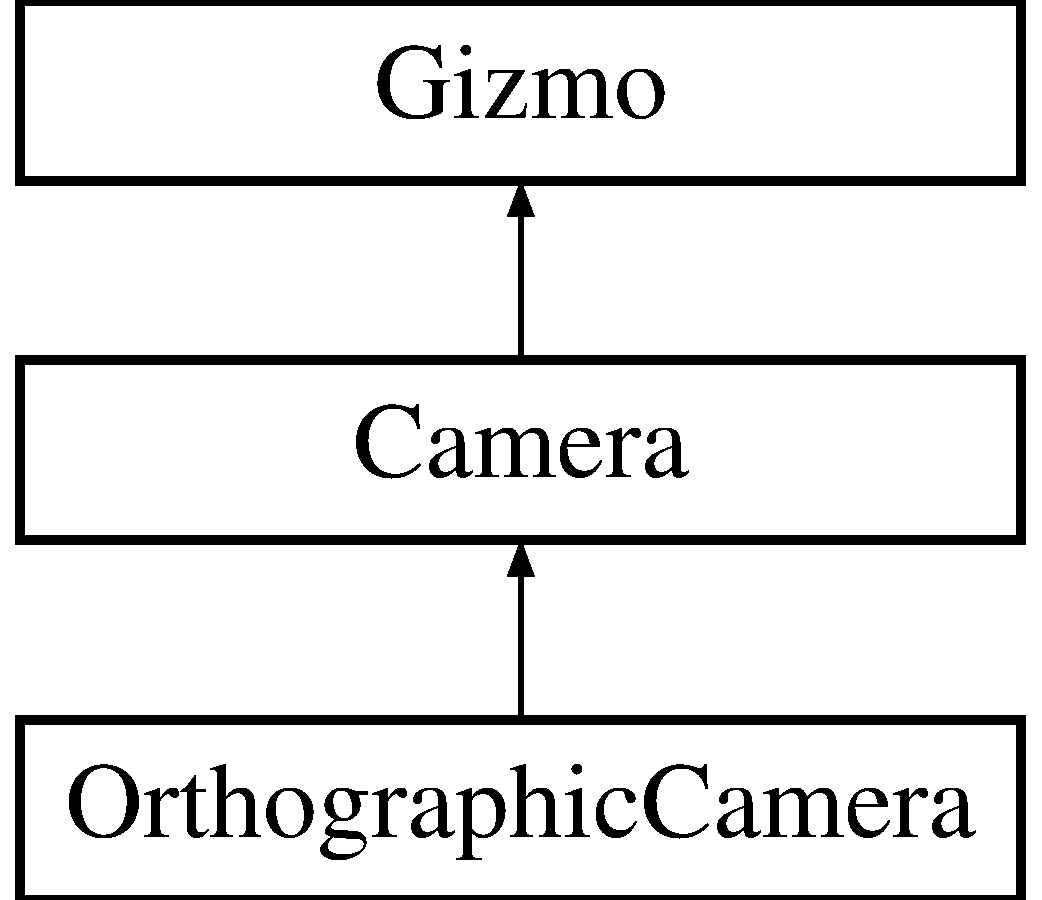
\includegraphics[height=3.000000cm]{class_orthographic_camera}
\end{center}
\end{figure}
\subsection*{Public Member Functions}
\begin{DoxyCompactItemize}
\item 
\hyperlink{class_orthographic_camera_a794762aa66ade1f025ca62304b2e8c40}{Orthographic\+Camera} (float p\+Near\+Plane, float p\+Far\+Plane, glm\+::vec3 p\+Look\+At, glm\+::vec3 p\+Up, glm\+::vec3 p\+Position, float p\+Top, float p\+Bottom, float p\+Left, float p\+Right)
\begin{DoxyCompactList}\small\item\em Constructor. \end{DoxyCompactList}\item 
\hyperlink{class_orthographic_camera_a889267a0f4815b523b07034d656986de}{Orthographic\+Camera} (const \hyperlink{class_orthographic_camera}{Orthographic\+Camera} \&p\+Orthographic\+Camera)
\begin{DoxyCompactList}\small\item\em Copy constructor. \end{DoxyCompactList}\item 
\hyperlink{class_orthographic_camera_a9c8a9cc81e87af987c6fcda276bdd52d}{$\sim$\+Orthographic\+Camera} ()
\begin{DoxyCompactList}\small\item\em Destructor. \end{DoxyCompactList}\item 
void \hyperlink{class_orthographic_camera_abea153f1372b655f423679015d42af52}{Update\+Projection} ()
\begin{DoxyCompactList}\small\item\em Update the projection matrix. \end{DoxyCompactList}\item 
\hyperlink{class_orthographic_camera}{Orthographic\+Camera} $\ast$ \hyperlink{class_orthographic_camera_a31414e246ccb74590fe025a82f1f6bd5}{Clone} () const 
\begin{DoxyCompactList}\small\item\em Method to clone the camera. \end{DoxyCompactList}\item 
void \hyperlink{class_orthographic_camera_ad6f26cfe2311ed951562f6cb856f7b3a}{Set\+Top} (float p\+Top)
\begin{DoxyCompactList}\small\item\em Set the top value. \end{DoxyCompactList}\item 
void \hyperlink{class_orthographic_camera_aaa433e475cfbec1455f4dab5b3f5b224}{Set\+Bottom} (float p\+Bottom)
\begin{DoxyCompactList}\small\item\em Set the bottom value. \end{DoxyCompactList}\item 
void \hyperlink{class_orthographic_camera_addc3594ec0843b3936a6830de8f16a16}{Set\+Left} (float p\+Left)
\begin{DoxyCompactList}\small\item\em Set the left value. \end{DoxyCompactList}\item 
void \hyperlink{class_orthographic_camera_a361f95d002589579563791a2b6fcb1f0}{Set\+Right} (float p\+Right)
\begin{DoxyCompactList}\small\item\em Set the right value. \end{DoxyCompactList}\end{DoxyCompactItemize}
\subsection*{Private Member Functions}
\begin{DoxyCompactItemize}
\item 
void \hyperlink{class_orthographic_camera_a5edb0b3f645e77d086024157ef684eea}{Create\+Mesh} ()
\begin{DoxyCompactList}\small\item\em Create the mesh of the gizmo with the indexs, positions and colors. \end{DoxyCompactList}\item 
void \hyperlink{class_orthographic_camera_ad774f1e383f99a94e3f733ecaa814e80}{Update\+Positions} ()
\begin{DoxyCompactList}\small\item\em Update the positions of the vertices of the mesh. \end{DoxyCompactList}\end{DoxyCompactItemize}
\subsection*{Private Attributes}
\begin{DoxyCompactItemize}
\item 
float \hyperlink{class_orthographic_camera_adb391b0b57fa70a2eaadd661f8ab423d}{m\+Top}
\begin{DoxyCompactList}\small\item\em Top value. \end{DoxyCompactList}\item 
float \hyperlink{class_orthographic_camera_aa901bf30589a77235d3b583d7a549ea0}{m\+Bottom}
\begin{DoxyCompactList}\small\item\em Bottom value. \end{DoxyCompactList}\item 
float \hyperlink{class_orthographic_camera_a9a1ad18a4b2b39b4d3f7f09f53817d54}{m\+Left}
\begin{DoxyCompactList}\small\item\em Left value. \end{DoxyCompactList}\item 
float \hyperlink{class_orthographic_camera_a8ece912d753235b6f79f1607a19f892b}{m\+Right}
\begin{DoxyCompactList}\small\item\em Right value. \end{DoxyCompactList}\end{DoxyCompactItemize}
\subsection*{Additional Inherited Members}


\subsection{Detailed Description}
\hyperlink{class_camera}{Camera} class with methods to configure an orthographic camera. 

\begin{DoxyAuthor}{Author}
Xavier Bonaventura 

Nicolau Sunyer 

Copyright\+: (c) Universitat de Girona 
\end{DoxyAuthor}


\subsection{Constructor \& Destructor Documentation}
\hypertarget{class_orthographic_camera_a794762aa66ade1f025ca62304b2e8c40}{\index{Orthographic\+Camera@{Orthographic\+Camera}!Orthographic\+Camera@{Orthographic\+Camera}}
\index{Orthographic\+Camera@{Orthographic\+Camera}!Orthographic\+Camera@{Orthographic\+Camera}}
\subsubsection[{Orthographic\+Camera}]{\setlength{\rightskip}{0pt plus 5cm}Orthographic\+Camera\+::\+Orthographic\+Camera (
\begin{DoxyParamCaption}
\item[{float}]{p\+Near\+Plane, }
\item[{float}]{p\+Far\+Plane, }
\item[{glm\+::vec3}]{p\+Look\+At, }
\item[{glm\+::vec3}]{p\+Up, }
\item[{glm\+::vec3}]{p\+Position, }
\item[{float}]{p\+Top, }
\item[{float}]{p\+Bottom, }
\item[{float}]{p\+Left, }
\item[{float}]{p\+Right}
\end{DoxyParamCaption}
)}}\label{class_orthographic_camera_a794762aa66ade1f025ca62304b2e8c40}


Constructor. 

\hypertarget{class_orthographic_camera_a889267a0f4815b523b07034d656986de}{\index{Orthographic\+Camera@{Orthographic\+Camera}!Orthographic\+Camera@{Orthographic\+Camera}}
\index{Orthographic\+Camera@{Orthographic\+Camera}!Orthographic\+Camera@{Orthographic\+Camera}}
\subsubsection[{Orthographic\+Camera}]{\setlength{\rightskip}{0pt plus 5cm}Orthographic\+Camera\+::\+Orthographic\+Camera (
\begin{DoxyParamCaption}
\item[{const {\bf Orthographic\+Camera} \&}]{p\+Orthographic\+Camera}
\end{DoxyParamCaption}
)}}\label{class_orthographic_camera_a889267a0f4815b523b07034d656986de}


Copy constructor. 

\hypertarget{class_orthographic_camera_a9c8a9cc81e87af987c6fcda276bdd52d}{\index{Orthographic\+Camera@{Orthographic\+Camera}!````~Orthographic\+Camera@{$\sim$\+Orthographic\+Camera}}
\index{````~Orthographic\+Camera@{$\sim$\+Orthographic\+Camera}!Orthographic\+Camera@{Orthographic\+Camera}}
\subsubsection[{$\sim$\+Orthographic\+Camera}]{\setlength{\rightskip}{0pt plus 5cm}Orthographic\+Camera\+::$\sim$\+Orthographic\+Camera (
\begin{DoxyParamCaption}
{}
\end{DoxyParamCaption}
)}}\label{class_orthographic_camera_a9c8a9cc81e87af987c6fcda276bdd52d}


Destructor. 



\subsection{Member Function Documentation}
\hypertarget{class_orthographic_camera_a31414e246ccb74590fe025a82f1f6bd5}{\index{Orthographic\+Camera@{Orthographic\+Camera}!Clone@{Clone}}
\index{Clone@{Clone}!Orthographic\+Camera@{Orthographic\+Camera}}
\subsubsection[{Clone}]{\setlength{\rightskip}{0pt plus 5cm}{\bf Orthographic\+Camera} $\ast$ Orthographic\+Camera\+::\+Clone (
\begin{DoxyParamCaption}
{}
\end{DoxyParamCaption}
) const\hspace{0.3cm}{\ttfamily [virtual]}}}\label{class_orthographic_camera_a31414e246ccb74590fe025a82f1f6bd5}


Method to clone the camera. 



Implements \hyperlink{class_camera_a81df82c60ae1a1d32090433ebdd30628}{Camera}.

\hypertarget{class_orthographic_camera_a5edb0b3f645e77d086024157ef684eea}{\index{Orthographic\+Camera@{Orthographic\+Camera}!Create\+Mesh@{Create\+Mesh}}
\index{Create\+Mesh@{Create\+Mesh}!Orthographic\+Camera@{Orthographic\+Camera}}
\subsubsection[{Create\+Mesh}]{\setlength{\rightskip}{0pt plus 5cm}void Orthographic\+Camera\+::\+Create\+Mesh (
\begin{DoxyParamCaption}
{}
\end{DoxyParamCaption}
)\hspace{0.3cm}{\ttfamily [private]}, {\ttfamily [virtual]}}}\label{class_orthographic_camera_a5edb0b3f645e77d086024157ef684eea}


Create the mesh of the gizmo with the indexs, positions and colors. 

Creation of the mesh

Set the positions

Set the colors

Set the indexs 

Implements \hyperlink{class_gizmo_a4ba36c75e6b8c2f729792de0161f5532}{Gizmo}.

\hypertarget{class_orthographic_camera_aaa433e475cfbec1455f4dab5b3f5b224}{\index{Orthographic\+Camera@{Orthographic\+Camera}!Set\+Bottom@{Set\+Bottom}}
\index{Set\+Bottom@{Set\+Bottom}!Orthographic\+Camera@{Orthographic\+Camera}}
\subsubsection[{Set\+Bottom}]{\setlength{\rightskip}{0pt plus 5cm}void Orthographic\+Camera\+::\+Set\+Bottom (
\begin{DoxyParamCaption}
\item[{float}]{p\+Bottom}
\end{DoxyParamCaption}
)}}\label{class_orthographic_camera_aaa433e475cfbec1455f4dab5b3f5b224}


Set the bottom value. 

\hypertarget{class_orthographic_camera_addc3594ec0843b3936a6830de8f16a16}{\index{Orthographic\+Camera@{Orthographic\+Camera}!Set\+Left@{Set\+Left}}
\index{Set\+Left@{Set\+Left}!Orthographic\+Camera@{Orthographic\+Camera}}
\subsubsection[{Set\+Left}]{\setlength{\rightskip}{0pt plus 5cm}void Orthographic\+Camera\+::\+Set\+Left (
\begin{DoxyParamCaption}
\item[{float}]{p\+Left}
\end{DoxyParamCaption}
)}}\label{class_orthographic_camera_addc3594ec0843b3936a6830de8f16a16}


Set the left value. 

\hypertarget{class_orthographic_camera_a361f95d002589579563791a2b6fcb1f0}{\index{Orthographic\+Camera@{Orthographic\+Camera}!Set\+Right@{Set\+Right}}
\index{Set\+Right@{Set\+Right}!Orthographic\+Camera@{Orthographic\+Camera}}
\subsubsection[{Set\+Right}]{\setlength{\rightskip}{0pt plus 5cm}void Orthographic\+Camera\+::\+Set\+Right (
\begin{DoxyParamCaption}
\item[{float}]{p\+Right}
\end{DoxyParamCaption}
)}}\label{class_orthographic_camera_a361f95d002589579563791a2b6fcb1f0}


Set the right value. 

\hypertarget{class_orthographic_camera_ad6f26cfe2311ed951562f6cb856f7b3a}{\index{Orthographic\+Camera@{Orthographic\+Camera}!Set\+Top@{Set\+Top}}
\index{Set\+Top@{Set\+Top}!Orthographic\+Camera@{Orthographic\+Camera}}
\subsubsection[{Set\+Top}]{\setlength{\rightskip}{0pt plus 5cm}void Orthographic\+Camera\+::\+Set\+Top (
\begin{DoxyParamCaption}
\item[{float}]{p\+Top}
\end{DoxyParamCaption}
)}}\label{class_orthographic_camera_ad6f26cfe2311ed951562f6cb856f7b3a}


Set the top value. 

\hypertarget{class_orthographic_camera_ad774f1e383f99a94e3f733ecaa814e80}{\index{Orthographic\+Camera@{Orthographic\+Camera}!Update\+Positions@{Update\+Positions}}
\index{Update\+Positions@{Update\+Positions}!Orthographic\+Camera@{Orthographic\+Camera}}
\subsubsection[{Update\+Positions}]{\setlength{\rightskip}{0pt plus 5cm}void Orthographic\+Camera\+::\+Update\+Positions (
\begin{DoxyParamCaption}
{}
\end{DoxyParamCaption}
)\hspace{0.3cm}{\ttfamily [private]}, {\ttfamily [virtual]}}}\label{class_orthographic_camera_ad774f1e383f99a94e3f733ecaa814e80}


Update the positions of the vertices of the mesh. 



Implements \hyperlink{class_gizmo_a30161525d80402eb0653f2612003a733}{Gizmo}.

\hypertarget{class_orthographic_camera_abea153f1372b655f423679015d42af52}{\index{Orthographic\+Camera@{Orthographic\+Camera}!Update\+Projection@{Update\+Projection}}
\index{Update\+Projection@{Update\+Projection}!Orthographic\+Camera@{Orthographic\+Camera}}
\subsubsection[{Update\+Projection}]{\setlength{\rightskip}{0pt plus 5cm}void Orthographic\+Camera\+::\+Update\+Projection (
\begin{DoxyParamCaption}
{}
\end{DoxyParamCaption}
)\hspace{0.3cm}{\ttfamily [virtual]}}}\label{class_orthographic_camera_abea153f1372b655f423679015d42af52}


Update the projection matrix. 



Implements \hyperlink{class_camera_a199f2379e1a1603da6cca9fe0162626d}{Camera}.



\subsection{Member Data Documentation}
\hypertarget{class_orthographic_camera_aa901bf30589a77235d3b583d7a549ea0}{\index{Orthographic\+Camera@{Orthographic\+Camera}!m\+Bottom@{m\+Bottom}}
\index{m\+Bottom@{m\+Bottom}!Orthographic\+Camera@{Orthographic\+Camera}}
\subsubsection[{m\+Bottom}]{\setlength{\rightskip}{0pt plus 5cm}float Orthographic\+Camera\+::m\+Bottom\hspace{0.3cm}{\ttfamily [private]}}}\label{class_orthographic_camera_aa901bf30589a77235d3b583d7a549ea0}


Bottom value. 

\hypertarget{class_orthographic_camera_a9a1ad18a4b2b39b4d3f7f09f53817d54}{\index{Orthographic\+Camera@{Orthographic\+Camera}!m\+Left@{m\+Left}}
\index{m\+Left@{m\+Left}!Orthographic\+Camera@{Orthographic\+Camera}}
\subsubsection[{m\+Left}]{\setlength{\rightskip}{0pt plus 5cm}float Orthographic\+Camera\+::m\+Left\hspace{0.3cm}{\ttfamily [private]}}}\label{class_orthographic_camera_a9a1ad18a4b2b39b4d3f7f09f53817d54}


Left value. 

\hypertarget{class_orthographic_camera_a8ece912d753235b6f79f1607a19f892b}{\index{Orthographic\+Camera@{Orthographic\+Camera}!m\+Right@{m\+Right}}
\index{m\+Right@{m\+Right}!Orthographic\+Camera@{Orthographic\+Camera}}
\subsubsection[{m\+Right}]{\setlength{\rightskip}{0pt plus 5cm}float Orthographic\+Camera\+::m\+Right\hspace{0.3cm}{\ttfamily [private]}}}\label{class_orthographic_camera_a8ece912d753235b6f79f1607a19f892b}


Right value. 

\hypertarget{class_orthographic_camera_adb391b0b57fa70a2eaadd661f8ab423d}{\index{Orthographic\+Camera@{Orthographic\+Camera}!m\+Top@{m\+Top}}
\index{m\+Top@{m\+Top}!Orthographic\+Camera@{Orthographic\+Camera}}
\subsubsection[{m\+Top}]{\setlength{\rightskip}{0pt plus 5cm}float Orthographic\+Camera\+::m\+Top\hspace{0.3cm}{\ttfamily [private]}}}\label{class_orthographic_camera_adb391b0b57fa70a2eaadd661f8ab423d}


Top value. 



The documentation for this class was generated from the following files\+:\begin{DoxyCompactItemize}
\item 
inc/core/\hyperlink{_orthographic_camera_8h}{Orthographic\+Camera.\+h}\item 
src/core/\hyperlink{_orthographic_camera_8cpp}{Orthographic\+Camera.\+cpp}\end{DoxyCompactItemize}

\hypertarget{class_perspective_camera}{\section{Perspective\+Camera Class Reference}
\label{class_perspective_camera}\index{Perspective\+Camera@{Perspective\+Camera}}
}


\hyperlink{class_camera}{Camera} class with methods to configure a perspective camera.  




{\ttfamily \#include $<$Perspective\+Camera.\+h$>$}

Inheritance diagram for Perspective\+Camera\+:\begin{figure}[H]
\begin{center}
\leavevmode
\includegraphics[height=3.000000cm]{class_perspective_camera}
\end{center}
\end{figure}
\subsection*{Public Member Functions}
\begin{DoxyCompactItemize}
\item 
\hyperlink{class_perspective_camera_a701bf1d9090bb34a960d152ed85f1f5c}{Perspective\+Camera} (float p\+Near\+Plane, float p\+Far\+Plane, glm\+::vec3 p\+Look\+At, glm\+::vec3 p\+Up, glm\+::vec3 p\+Position, float p\+Angle, float p\+Aspect\+Ratio)
\begin{DoxyCompactList}\small\item\em Constructor. \end{DoxyCompactList}\item 
\hyperlink{class_perspective_camera_adfe834fa0ca591dd84a4785f594d8ba9}{Perspective\+Camera} (const \hyperlink{class_perspective_camera}{Perspective\+Camera} \&p\+Perspective\+Camera)
\begin{DoxyCompactList}\small\item\em Copy constructor. \end{DoxyCompactList}\item 
\hyperlink{class_perspective_camera_a935a64c478ab072bb9ba050b7d388526}{$\sim$\+Perspective\+Camera} ()
\begin{DoxyCompactList}\small\item\em Destructor. \end{DoxyCompactList}\item 
void \hyperlink{class_perspective_camera_acffce4415501bb3839f8e50a22465169}{Update\+Projection} ()
\begin{DoxyCompactList}\small\item\em Update the projection matrix. \end{DoxyCompactList}\item 
\hyperlink{class_perspective_camera}{Perspective\+Camera} $\ast$ \hyperlink{class_perspective_camera_a551b2bb8f13d7f89b2459436f6b275fb}{Clone} () const 
\begin{DoxyCompactList}\small\item\em Method to clone the camera. \end{DoxyCompactList}\item 
void \hyperlink{class_perspective_camera_a7e581143f69d58edc94ddc224f29971c}{Set\+Angle} (float p\+Angle)
\begin{DoxyCompactList}\small\item\em Set the field of view angle. \end{DoxyCompactList}\item 
float \hyperlink{class_perspective_camera_a7ed08d265308466003b674ab535823ce}{Get\+Angle} () const 
\begin{DoxyCompactList}\small\item\em Get the field of view angle. \end{DoxyCompactList}\end{DoxyCompactItemize}
\subsection*{Protected Member Functions}
\begin{DoxyCompactItemize}
\item 
void \hyperlink{class_perspective_camera_acefab56b5bf9449e1a97e0f193702d36}{Create\+Mesh} ()
\begin{DoxyCompactList}\small\item\em Create the mesh of the gizmo with the indexs, positions and colors. \end{DoxyCompactList}\item 
void \hyperlink{class_perspective_camera_a80ca50f210c1ea07f346bcee9dff6451}{Update\+Positions} ()
\begin{DoxyCompactList}\small\item\em Update the positions of the vertices of the mesh. \end{DoxyCompactList}\end{DoxyCompactItemize}
\subsection*{Protected Attributes}
\begin{DoxyCompactItemize}
\item 
float \hyperlink{class_perspective_camera_ada0d00e4ec22629c55df5ab0af4a3857}{m\+Angle}
\begin{DoxyCompactList}\small\item\em Field of view angle. \end{DoxyCompactList}\end{DoxyCompactItemize}
\subsection*{Additional Inherited Members}


\subsection{Detailed Description}
\hyperlink{class_camera}{Camera} class with methods to configure a perspective camera. 

\begin{DoxyAuthor}{Author}
Xavier Bonaventura 

Nicolau Sunyer 

Copyright\+: (c) Universitat de Girona 
\end{DoxyAuthor}


\subsection{Constructor \& Destructor Documentation}
\hypertarget{class_perspective_camera_a701bf1d9090bb34a960d152ed85f1f5c}{\index{Perspective\+Camera@{Perspective\+Camera}!Perspective\+Camera@{Perspective\+Camera}}
\index{Perspective\+Camera@{Perspective\+Camera}!Perspective\+Camera@{Perspective\+Camera}}
\subsubsection[{Perspective\+Camera}]{\setlength{\rightskip}{0pt plus 5cm}Perspective\+Camera\+::\+Perspective\+Camera (
\begin{DoxyParamCaption}
\item[{float}]{p\+Near\+Plane, }
\item[{float}]{p\+Far\+Plane, }
\item[{glm\+::vec3}]{p\+Look\+At, }
\item[{glm\+::vec3}]{p\+Up, }
\item[{glm\+::vec3}]{p\+Position, }
\item[{float}]{p\+Angle, }
\item[{float}]{p\+Aspect\+Ratio}
\end{DoxyParamCaption}
)}}\label{class_perspective_camera_a701bf1d9090bb34a960d152ed85f1f5c}


Constructor. 

\hypertarget{class_perspective_camera_adfe834fa0ca591dd84a4785f594d8ba9}{\index{Perspective\+Camera@{Perspective\+Camera}!Perspective\+Camera@{Perspective\+Camera}}
\index{Perspective\+Camera@{Perspective\+Camera}!Perspective\+Camera@{Perspective\+Camera}}
\subsubsection[{Perspective\+Camera}]{\setlength{\rightskip}{0pt plus 5cm}Perspective\+Camera\+::\+Perspective\+Camera (
\begin{DoxyParamCaption}
\item[{const {\bf Perspective\+Camera} \&}]{p\+Perspective\+Camera}
\end{DoxyParamCaption}
)}}\label{class_perspective_camera_adfe834fa0ca591dd84a4785f594d8ba9}


Copy constructor. 

\hypertarget{class_perspective_camera_a935a64c478ab072bb9ba050b7d388526}{\index{Perspective\+Camera@{Perspective\+Camera}!````~Perspective\+Camera@{$\sim$\+Perspective\+Camera}}
\index{````~Perspective\+Camera@{$\sim$\+Perspective\+Camera}!Perspective\+Camera@{Perspective\+Camera}}
\subsubsection[{$\sim$\+Perspective\+Camera}]{\setlength{\rightskip}{0pt plus 5cm}Perspective\+Camera\+::$\sim$\+Perspective\+Camera (
\begin{DoxyParamCaption}
{}
\end{DoxyParamCaption}
)}}\label{class_perspective_camera_a935a64c478ab072bb9ba050b7d388526}


Destructor. 



\subsection{Member Function Documentation}
\hypertarget{class_perspective_camera_a551b2bb8f13d7f89b2459436f6b275fb}{\index{Perspective\+Camera@{Perspective\+Camera}!Clone@{Clone}}
\index{Clone@{Clone}!Perspective\+Camera@{Perspective\+Camera}}
\subsubsection[{Clone}]{\setlength{\rightskip}{0pt plus 5cm}{\bf Perspective\+Camera} $\ast$ Perspective\+Camera\+::\+Clone (
\begin{DoxyParamCaption}
{}
\end{DoxyParamCaption}
) const\hspace{0.3cm}{\ttfamily [virtual]}}}\label{class_perspective_camera_a551b2bb8f13d7f89b2459436f6b275fb}


Method to clone the camera. 



Implements \hyperlink{class_camera_a81df82c60ae1a1d32090433ebdd30628}{Camera}.

\hypertarget{class_perspective_camera_acefab56b5bf9449e1a97e0f193702d36}{\index{Perspective\+Camera@{Perspective\+Camera}!Create\+Mesh@{Create\+Mesh}}
\index{Create\+Mesh@{Create\+Mesh}!Perspective\+Camera@{Perspective\+Camera}}
\subsubsection[{Create\+Mesh}]{\setlength{\rightskip}{0pt plus 5cm}void Perspective\+Camera\+::\+Create\+Mesh (
\begin{DoxyParamCaption}
{}
\end{DoxyParamCaption}
)\hspace{0.3cm}{\ttfamily [protected]}, {\ttfamily [virtual]}}}\label{class_perspective_camera_acefab56b5bf9449e1a97e0f193702d36}


Create the mesh of the gizmo with the indexs, positions and colors. 

Creation of the mesh

Set the positions

Set the colors

Set the indexs 

Implements \hyperlink{class_gizmo_a4ba36c75e6b8c2f729792de0161f5532}{Gizmo}.

\hypertarget{class_perspective_camera_a7ed08d265308466003b674ab535823ce}{\index{Perspective\+Camera@{Perspective\+Camera}!Get\+Angle@{Get\+Angle}}
\index{Get\+Angle@{Get\+Angle}!Perspective\+Camera@{Perspective\+Camera}}
\subsubsection[{Get\+Angle}]{\setlength{\rightskip}{0pt plus 5cm}float Perspective\+Camera\+::\+Get\+Angle (
\begin{DoxyParamCaption}
{}
\end{DoxyParamCaption}
) const}}\label{class_perspective_camera_a7ed08d265308466003b674ab535823ce}


Get the field of view angle. 

\hypertarget{class_perspective_camera_a7e581143f69d58edc94ddc224f29971c}{\index{Perspective\+Camera@{Perspective\+Camera}!Set\+Angle@{Set\+Angle}}
\index{Set\+Angle@{Set\+Angle}!Perspective\+Camera@{Perspective\+Camera}}
\subsubsection[{Set\+Angle}]{\setlength{\rightskip}{0pt plus 5cm}void Perspective\+Camera\+::\+Set\+Angle (
\begin{DoxyParamCaption}
\item[{float}]{p\+Angle}
\end{DoxyParamCaption}
)}}\label{class_perspective_camera_a7e581143f69d58edc94ddc224f29971c}


Set the field of view angle. 

\hypertarget{class_perspective_camera_a80ca50f210c1ea07f346bcee9dff6451}{\index{Perspective\+Camera@{Perspective\+Camera}!Update\+Positions@{Update\+Positions}}
\index{Update\+Positions@{Update\+Positions}!Perspective\+Camera@{Perspective\+Camera}}
\subsubsection[{Update\+Positions}]{\setlength{\rightskip}{0pt plus 5cm}void Perspective\+Camera\+::\+Update\+Positions (
\begin{DoxyParamCaption}
{}
\end{DoxyParamCaption}
)\hspace{0.3cm}{\ttfamily [protected]}, {\ttfamily [virtual]}}}\label{class_perspective_camera_a80ca50f210c1ea07f346bcee9dff6451}


Update the positions of the vertices of the mesh. 



Implements \hyperlink{class_gizmo_a30161525d80402eb0653f2612003a733}{Gizmo}.

\hypertarget{class_perspective_camera_acffce4415501bb3839f8e50a22465169}{\index{Perspective\+Camera@{Perspective\+Camera}!Update\+Projection@{Update\+Projection}}
\index{Update\+Projection@{Update\+Projection}!Perspective\+Camera@{Perspective\+Camera}}
\subsubsection[{Update\+Projection}]{\setlength{\rightskip}{0pt plus 5cm}void Perspective\+Camera\+::\+Update\+Projection (
\begin{DoxyParamCaption}
{}
\end{DoxyParamCaption}
)\hspace{0.3cm}{\ttfamily [virtual]}}}\label{class_perspective_camera_acffce4415501bb3839f8e50a22465169}


Update the projection matrix. 



Implements \hyperlink{class_camera_a199f2379e1a1603da6cca9fe0162626d}{Camera}.



\subsection{Member Data Documentation}
\hypertarget{class_perspective_camera_ada0d00e4ec22629c55df5ab0af4a3857}{\index{Perspective\+Camera@{Perspective\+Camera}!m\+Angle@{m\+Angle}}
\index{m\+Angle@{m\+Angle}!Perspective\+Camera@{Perspective\+Camera}}
\subsubsection[{m\+Angle}]{\setlength{\rightskip}{0pt plus 5cm}float Perspective\+Camera\+::m\+Angle\hspace{0.3cm}{\ttfamily [protected]}}}\label{class_perspective_camera_ada0d00e4ec22629c55df5ab0af4a3857}


Field of view angle. 



The documentation for this class was generated from the following files\+:\begin{DoxyCompactItemize}
\item 
inc/core/\hyperlink{_perspective_camera_8h}{Perspective\+Camera.\+h}\item 
src/core/\hyperlink{_perspective_camera_8cpp}{Perspective\+Camera.\+cpp}\end{DoxyCompactItemize}

\hypertarget{class_projected_area}{\section{Projected\+Area Class Reference}
\label{class_projected_area}\index{Projected\+Area@{Projected\+Area}}
}


Class that implements the projected area measure.  




{\ttfamily \#include $<$Projected\+Area.\+h$>$}

Inheritance diagram for Projected\+Area\+:\begin{figure}[H]
\begin{center}
\leavevmode
\includegraphics[height=2.000000cm]{class_projected_area}
\end{center}
\end{figure}
\subsection*{Public Member Functions}
\begin{DoxyCompactItemize}
\item 
\hyperlink{class_projected_area_aa033c0455632352ccf150482773f37cd}{Projected\+Area} (const Q\+String \&p\+Name)
\begin{DoxyCompactList}\small\item\em Constructor. \end{DoxyCompactList}\item 
\hyperlink{class_projected_area_a63ec33cc3105dd939a24346fd0aeafb5}{$\sim$\+Projected\+Area} ()
\begin{DoxyCompactList}\small\item\em Destructor. \end{DoxyCompactList}\item 
void \hyperlink{class_projected_area_ae035110fffb317c4c90785b96e23388c}{Compute} (const \hyperlink{class_scene_information_builder}{Scene\+Information\+Builder} $\ast$p\+Scene\+Information\+Builder)
\begin{DoxyCompactList}\small\item\em Method that computes the measure. \end{DoxyCompactList}\end{DoxyCompactItemize}
\subsection*{Additional Inherited Members}


\subsection{Detailed Description}
Class that implements the projected area measure. 

\begin{DoxyAuthor}{Author}
Xavier Bonaventura 

Copyright\+: (c) Universitat de Girona 
\end{DoxyAuthor}


\subsection{Constructor \& Destructor Documentation}
\hypertarget{class_projected_area_aa033c0455632352ccf150482773f37cd}{\index{Projected\+Area@{Projected\+Area}!Projected\+Area@{Projected\+Area}}
\index{Projected\+Area@{Projected\+Area}!Projected\+Area@{Projected\+Area}}
\subsubsection[{Projected\+Area}]{\setlength{\rightskip}{0pt plus 5cm}Projected\+Area\+::\+Projected\+Area (
\begin{DoxyParamCaption}
\item[{const Q\+String \&}]{p\+Name}
\end{DoxyParamCaption}
)}}\label{class_projected_area_aa033c0455632352ccf150482773f37cd}


Constructor. 

\hypertarget{class_projected_area_a63ec33cc3105dd939a24346fd0aeafb5}{\index{Projected\+Area@{Projected\+Area}!````~Projected\+Area@{$\sim$\+Projected\+Area}}
\index{````~Projected\+Area@{$\sim$\+Projected\+Area}!Projected\+Area@{Projected\+Area}}
\subsubsection[{$\sim$\+Projected\+Area}]{\setlength{\rightskip}{0pt plus 5cm}Projected\+Area\+::$\sim$\+Projected\+Area (
\begin{DoxyParamCaption}
{}
\end{DoxyParamCaption}
)}}\label{class_projected_area_a63ec33cc3105dd939a24346fd0aeafb5}


Destructor. 



\subsection{Member Function Documentation}
\hypertarget{class_projected_area_ae035110fffb317c4c90785b96e23388c}{\index{Projected\+Area@{Projected\+Area}!Compute@{Compute}}
\index{Compute@{Compute}!Projected\+Area@{Projected\+Area}}
\subsubsection[{Compute}]{\setlength{\rightskip}{0pt plus 5cm}void Projected\+Area\+::\+Compute (
\begin{DoxyParamCaption}
\item[{const {\bf Scene\+Information\+Builder} $\ast$}]{p\+Scene\+Information\+Builder}
\end{DoxyParamCaption}
)\hspace{0.3cm}{\ttfamily [virtual]}}}\label{class_projected_area_ae035110fffb317c4c90785b96e23388c}


Method that computes the measure. 



Implements \hyperlink{class_measure_aed88fe46b2a609ab5948e5f3c891321d}{Measure}.



The documentation for this class was generated from the following files\+:\begin{DoxyCompactItemize}
\item 
inc/viewpoint-\/measures/\hyperlink{_projected_area_8h}{Projected\+Area.\+h}\item 
src/viewpoint-\/measures/\hyperlink{_projected_area_8cpp}{Projected\+Area.\+cpp}\end{DoxyCompactItemize}

\hypertarget{class_projected_areas_matrix}{\section{Projected\+Areas\+Matrix Class Reference}
\label{class_projected_areas_matrix}\index{Projected\+Areas\+Matrix@{Projected\+Areas\+Matrix}}
}


{\ttfamily \#include $<$Projected\+Areas\+Matrix.\+h$>$}

\subsection*{Public Member Functions}
\begin{DoxyCompactItemize}
\item 
\hyperlink{class_projected_areas_matrix_a129e6c7a93c2c8d69a258399fa725be4}{Projected\+Areas\+Matrix} (int p\+Number\+Of\+Viewpoints, int p\+Number\+Of\+Polygons)
\item 
\hyperlink{class_projected_areas_matrix_a44019a731f9d882bd72f4498cfbb35a0}{Projected\+Areas\+Matrix} (const \hyperlink{class_projected_areas_matrix}{Projected\+Areas\+Matrix} $\ast$p\+Projected\+Areas\+Matrix)
\item 
int \hyperlink{class_projected_areas_matrix_a67f41fd64b2e0909a19751c7a6adb520}{Get\+Number\+Of\+Viewpoints} () const 
\item 
int \hyperlink{class_projected_areas_matrix_a3a33b7776927250d46e48010096b6f5d}{Get\+Number\+Of\+Polygons} () const 
\item 
unsigned int \hyperlink{class_projected_areas_matrix_a24b7121f91cf87060a15f35d146d4fad}{Get\+Sum\+Per\+Viewpoint} (int p\+Viewpoint) const 
\item 
unsigned int \hyperlink{class_projected_areas_matrix_aae702f18b408ad2798310307119f0efb}{Get\+Sum\+Per\+Polygon} (int p\+Polygon) const 
\item 
unsigned int \hyperlink{class_projected_areas_matrix_a94900bb0cb32473fea98baff3f97f804}{Get\+Total\+Sum} () const 
\item 
void \hyperlink{class_projected_areas_matrix_ab7dca98fc4d6eba761074872d0520567}{Set\+Values} (int p\+Viewpoint, const Q\+Vector$<$ unsigned int $>$ \&p\+Values)
\item 
unsigned int \hyperlink{class_projected_areas_matrix_a0df4213a8b8aaefe466631388f7dfaa8}{Get\+Value} (int p\+Viewpoint, int p\+Polygon) const 
\item 
void \hyperlink{class_projected_areas_matrix_a7c63a0e48e51d2a63abeb470373e86a7}{Compute} ()
\item 
void \hyperlink{class_projected_areas_matrix_a383a312b1ca476c968db47ac1a28d129}{Save\+To\+File} () const 
\end{DoxyCompactItemize}
\subsection*{Private Attributes}
\begin{DoxyCompactItemize}
\item 
Q\+Vector$<$ Q\+Vector$<$ unsigned int $>$ $>$ \hyperlink{class_projected_areas_matrix_ac47120ea675fc0153e7ee8a05d4a7ac6}{m\+Values}
\item 
int \hyperlink{class_projected_areas_matrix_a392583dc3a94e28e070e652a38b92076}{m\+Number\+Of\+Viewpoints}
\item 
int \hyperlink{class_projected_areas_matrix_a7b6677b16763d126f451e44b5aa98711}{m\+Number\+Of\+Polygons}
\item 
Q\+Vector$<$ unsigned int $>$ \hyperlink{class_projected_areas_matrix_a1eb9055173a5a45b00f560f33f20bd6f}{m\+Sum\+Per\+Viewpoint}
\item 
Q\+Vector$<$ unsigned int $>$ \hyperlink{class_projected_areas_matrix_afe1ccde064a456030a532b3e3ff9d72b}{m\+Sum\+Per\+Polygon}
\item 
unsigned int \hyperlink{class_projected_areas_matrix_a5cc3d0fedfb1071ea8849511050e3379}{m\+Total\+Sum}
\end{DoxyCompactItemize}


\subsection{Detailed Description}
\begin{DoxyAuthor}{Author}
Xavier Bonaventura 

Copyright\+: (c) Universitat de Girona 
\end{DoxyAuthor}


\subsection{Constructor \& Destructor Documentation}
\hypertarget{class_projected_areas_matrix_a129e6c7a93c2c8d69a258399fa725be4}{\index{Projected\+Areas\+Matrix@{Projected\+Areas\+Matrix}!Projected\+Areas\+Matrix@{Projected\+Areas\+Matrix}}
\index{Projected\+Areas\+Matrix@{Projected\+Areas\+Matrix}!Projected\+Areas\+Matrix@{Projected\+Areas\+Matrix}}
\subsubsection[{Projected\+Areas\+Matrix}]{\setlength{\rightskip}{0pt plus 5cm}Projected\+Areas\+Matrix\+::\+Projected\+Areas\+Matrix (
\begin{DoxyParamCaption}
\item[{int}]{p\+Number\+Of\+Viewpoints, }
\item[{int}]{p\+Number\+Of\+Polygons}
\end{DoxyParamCaption}
)}}\label{class_projected_areas_matrix_a129e6c7a93c2c8d69a258399fa725be4}
\hypertarget{class_projected_areas_matrix_a44019a731f9d882bd72f4498cfbb35a0}{\index{Projected\+Areas\+Matrix@{Projected\+Areas\+Matrix}!Projected\+Areas\+Matrix@{Projected\+Areas\+Matrix}}
\index{Projected\+Areas\+Matrix@{Projected\+Areas\+Matrix}!Projected\+Areas\+Matrix@{Projected\+Areas\+Matrix}}
\subsubsection[{Projected\+Areas\+Matrix}]{\setlength{\rightskip}{0pt plus 5cm}Projected\+Areas\+Matrix\+::\+Projected\+Areas\+Matrix (
\begin{DoxyParamCaption}
\item[{const {\bf Projected\+Areas\+Matrix} $\ast$}]{p\+Projected\+Areas\+Matrix}
\end{DoxyParamCaption}
)}}\label{class_projected_areas_matrix_a44019a731f9d882bd72f4498cfbb35a0}


\subsection{Member Function Documentation}
\hypertarget{class_projected_areas_matrix_a7c63a0e48e51d2a63abeb470373e86a7}{\index{Projected\+Areas\+Matrix@{Projected\+Areas\+Matrix}!Compute@{Compute}}
\index{Compute@{Compute}!Projected\+Areas\+Matrix@{Projected\+Areas\+Matrix}}
\subsubsection[{Compute}]{\setlength{\rightskip}{0pt plus 5cm}void Projected\+Areas\+Matrix\+::\+Compute (
\begin{DoxyParamCaption}
{}
\end{DoxyParamCaption}
)}}\label{class_projected_areas_matrix_a7c63a0e48e51d2a63abeb470373e86a7}
\hypertarget{class_projected_areas_matrix_a3a33b7776927250d46e48010096b6f5d}{\index{Projected\+Areas\+Matrix@{Projected\+Areas\+Matrix}!Get\+Number\+Of\+Polygons@{Get\+Number\+Of\+Polygons}}
\index{Get\+Number\+Of\+Polygons@{Get\+Number\+Of\+Polygons}!Projected\+Areas\+Matrix@{Projected\+Areas\+Matrix}}
\subsubsection[{Get\+Number\+Of\+Polygons}]{\setlength{\rightskip}{0pt plus 5cm}int Projected\+Areas\+Matrix\+::\+Get\+Number\+Of\+Polygons (
\begin{DoxyParamCaption}
{}
\end{DoxyParamCaption}
) const}}\label{class_projected_areas_matrix_a3a33b7776927250d46e48010096b6f5d}
\hypertarget{class_projected_areas_matrix_a67f41fd64b2e0909a19751c7a6adb520}{\index{Projected\+Areas\+Matrix@{Projected\+Areas\+Matrix}!Get\+Number\+Of\+Viewpoints@{Get\+Number\+Of\+Viewpoints}}
\index{Get\+Number\+Of\+Viewpoints@{Get\+Number\+Of\+Viewpoints}!Projected\+Areas\+Matrix@{Projected\+Areas\+Matrix}}
\subsubsection[{Get\+Number\+Of\+Viewpoints}]{\setlength{\rightskip}{0pt plus 5cm}int Projected\+Areas\+Matrix\+::\+Get\+Number\+Of\+Viewpoints (
\begin{DoxyParamCaption}
{}
\end{DoxyParamCaption}
) const}}\label{class_projected_areas_matrix_a67f41fd64b2e0909a19751c7a6adb520}
\hypertarget{class_projected_areas_matrix_aae702f18b408ad2798310307119f0efb}{\index{Projected\+Areas\+Matrix@{Projected\+Areas\+Matrix}!Get\+Sum\+Per\+Polygon@{Get\+Sum\+Per\+Polygon}}
\index{Get\+Sum\+Per\+Polygon@{Get\+Sum\+Per\+Polygon}!Projected\+Areas\+Matrix@{Projected\+Areas\+Matrix}}
\subsubsection[{Get\+Sum\+Per\+Polygon}]{\setlength{\rightskip}{0pt plus 5cm}unsigned int Projected\+Areas\+Matrix\+::\+Get\+Sum\+Per\+Polygon (
\begin{DoxyParamCaption}
\item[{int}]{p\+Polygon}
\end{DoxyParamCaption}
) const}}\label{class_projected_areas_matrix_aae702f18b408ad2798310307119f0efb}
\hypertarget{class_projected_areas_matrix_a24b7121f91cf87060a15f35d146d4fad}{\index{Projected\+Areas\+Matrix@{Projected\+Areas\+Matrix}!Get\+Sum\+Per\+Viewpoint@{Get\+Sum\+Per\+Viewpoint}}
\index{Get\+Sum\+Per\+Viewpoint@{Get\+Sum\+Per\+Viewpoint}!Projected\+Areas\+Matrix@{Projected\+Areas\+Matrix}}
\subsubsection[{Get\+Sum\+Per\+Viewpoint}]{\setlength{\rightskip}{0pt plus 5cm}unsigned int Projected\+Areas\+Matrix\+::\+Get\+Sum\+Per\+Viewpoint (
\begin{DoxyParamCaption}
\item[{int}]{p\+Viewpoint}
\end{DoxyParamCaption}
) const}}\label{class_projected_areas_matrix_a24b7121f91cf87060a15f35d146d4fad}
\hypertarget{class_projected_areas_matrix_a94900bb0cb32473fea98baff3f97f804}{\index{Projected\+Areas\+Matrix@{Projected\+Areas\+Matrix}!Get\+Total\+Sum@{Get\+Total\+Sum}}
\index{Get\+Total\+Sum@{Get\+Total\+Sum}!Projected\+Areas\+Matrix@{Projected\+Areas\+Matrix}}
\subsubsection[{Get\+Total\+Sum}]{\setlength{\rightskip}{0pt plus 5cm}unsigned int Projected\+Areas\+Matrix\+::\+Get\+Total\+Sum (
\begin{DoxyParamCaption}
{}
\end{DoxyParamCaption}
) const}}\label{class_projected_areas_matrix_a94900bb0cb32473fea98baff3f97f804}
\hypertarget{class_projected_areas_matrix_a0df4213a8b8aaefe466631388f7dfaa8}{\index{Projected\+Areas\+Matrix@{Projected\+Areas\+Matrix}!Get\+Value@{Get\+Value}}
\index{Get\+Value@{Get\+Value}!Projected\+Areas\+Matrix@{Projected\+Areas\+Matrix}}
\subsubsection[{Get\+Value}]{\setlength{\rightskip}{0pt plus 5cm}unsigned int Projected\+Areas\+Matrix\+::\+Get\+Value (
\begin{DoxyParamCaption}
\item[{int}]{p\+Viewpoint, }
\item[{int}]{p\+Polygon}
\end{DoxyParamCaption}
) const}}\label{class_projected_areas_matrix_a0df4213a8b8aaefe466631388f7dfaa8}
\hypertarget{class_projected_areas_matrix_a383a312b1ca476c968db47ac1a28d129}{\index{Projected\+Areas\+Matrix@{Projected\+Areas\+Matrix}!Save\+To\+File@{Save\+To\+File}}
\index{Save\+To\+File@{Save\+To\+File}!Projected\+Areas\+Matrix@{Projected\+Areas\+Matrix}}
\subsubsection[{Save\+To\+File}]{\setlength{\rightskip}{0pt plus 5cm}void Projected\+Areas\+Matrix\+::\+Save\+To\+File (
\begin{DoxyParamCaption}
{}
\end{DoxyParamCaption}
) const}}\label{class_projected_areas_matrix_a383a312b1ca476c968db47ac1a28d129}
\hypertarget{class_projected_areas_matrix_ab7dca98fc4d6eba761074872d0520567}{\index{Projected\+Areas\+Matrix@{Projected\+Areas\+Matrix}!Set\+Values@{Set\+Values}}
\index{Set\+Values@{Set\+Values}!Projected\+Areas\+Matrix@{Projected\+Areas\+Matrix}}
\subsubsection[{Set\+Values}]{\setlength{\rightskip}{0pt plus 5cm}void Projected\+Areas\+Matrix\+::\+Set\+Values (
\begin{DoxyParamCaption}
\item[{int}]{p\+Viewpoint, }
\item[{const Q\+Vector$<$ unsigned int $>$ \&}]{p\+Values}
\end{DoxyParamCaption}
)}}\label{class_projected_areas_matrix_ab7dca98fc4d6eba761074872d0520567}


\subsection{Member Data Documentation}
\hypertarget{class_projected_areas_matrix_a7b6677b16763d126f451e44b5aa98711}{\index{Projected\+Areas\+Matrix@{Projected\+Areas\+Matrix}!m\+Number\+Of\+Polygons@{m\+Number\+Of\+Polygons}}
\index{m\+Number\+Of\+Polygons@{m\+Number\+Of\+Polygons}!Projected\+Areas\+Matrix@{Projected\+Areas\+Matrix}}
\subsubsection[{m\+Number\+Of\+Polygons}]{\setlength{\rightskip}{0pt plus 5cm}int Projected\+Areas\+Matrix\+::m\+Number\+Of\+Polygons\hspace{0.3cm}{\ttfamily [private]}}}\label{class_projected_areas_matrix_a7b6677b16763d126f451e44b5aa98711}
\hypertarget{class_projected_areas_matrix_a392583dc3a94e28e070e652a38b92076}{\index{Projected\+Areas\+Matrix@{Projected\+Areas\+Matrix}!m\+Number\+Of\+Viewpoints@{m\+Number\+Of\+Viewpoints}}
\index{m\+Number\+Of\+Viewpoints@{m\+Number\+Of\+Viewpoints}!Projected\+Areas\+Matrix@{Projected\+Areas\+Matrix}}
\subsubsection[{m\+Number\+Of\+Viewpoints}]{\setlength{\rightskip}{0pt plus 5cm}int Projected\+Areas\+Matrix\+::m\+Number\+Of\+Viewpoints\hspace{0.3cm}{\ttfamily [private]}}}\label{class_projected_areas_matrix_a392583dc3a94e28e070e652a38b92076}
\hypertarget{class_projected_areas_matrix_afe1ccde064a456030a532b3e3ff9d72b}{\index{Projected\+Areas\+Matrix@{Projected\+Areas\+Matrix}!m\+Sum\+Per\+Polygon@{m\+Sum\+Per\+Polygon}}
\index{m\+Sum\+Per\+Polygon@{m\+Sum\+Per\+Polygon}!Projected\+Areas\+Matrix@{Projected\+Areas\+Matrix}}
\subsubsection[{m\+Sum\+Per\+Polygon}]{\setlength{\rightskip}{0pt plus 5cm}Q\+Vector$<$ unsigned int $>$ Projected\+Areas\+Matrix\+::m\+Sum\+Per\+Polygon\hspace{0.3cm}{\ttfamily [private]}}}\label{class_projected_areas_matrix_afe1ccde064a456030a532b3e3ff9d72b}
\hypertarget{class_projected_areas_matrix_a1eb9055173a5a45b00f560f33f20bd6f}{\index{Projected\+Areas\+Matrix@{Projected\+Areas\+Matrix}!m\+Sum\+Per\+Viewpoint@{m\+Sum\+Per\+Viewpoint}}
\index{m\+Sum\+Per\+Viewpoint@{m\+Sum\+Per\+Viewpoint}!Projected\+Areas\+Matrix@{Projected\+Areas\+Matrix}}
\subsubsection[{m\+Sum\+Per\+Viewpoint}]{\setlength{\rightskip}{0pt plus 5cm}Q\+Vector$<$ unsigned int $>$ Projected\+Areas\+Matrix\+::m\+Sum\+Per\+Viewpoint\hspace{0.3cm}{\ttfamily [private]}}}\label{class_projected_areas_matrix_a1eb9055173a5a45b00f560f33f20bd6f}
\hypertarget{class_projected_areas_matrix_a5cc3d0fedfb1071ea8849511050e3379}{\index{Projected\+Areas\+Matrix@{Projected\+Areas\+Matrix}!m\+Total\+Sum@{m\+Total\+Sum}}
\index{m\+Total\+Sum@{m\+Total\+Sum}!Projected\+Areas\+Matrix@{Projected\+Areas\+Matrix}}
\subsubsection[{m\+Total\+Sum}]{\setlength{\rightskip}{0pt plus 5cm}unsigned int Projected\+Areas\+Matrix\+::m\+Total\+Sum\hspace{0.3cm}{\ttfamily [private]}}}\label{class_projected_areas_matrix_a5cc3d0fedfb1071ea8849511050e3379}
\hypertarget{class_projected_areas_matrix_ac47120ea675fc0153e7ee8a05d4a7ac6}{\index{Projected\+Areas\+Matrix@{Projected\+Areas\+Matrix}!m\+Values@{m\+Values}}
\index{m\+Values@{m\+Values}!Projected\+Areas\+Matrix@{Projected\+Areas\+Matrix}}
\subsubsection[{m\+Values}]{\setlength{\rightskip}{0pt plus 5cm}Q\+Vector$<$ Q\+Vector$<$ unsigned int $>$ $>$ Projected\+Areas\+Matrix\+::m\+Values\hspace{0.3cm}{\ttfamily [private]}}}\label{class_projected_areas_matrix_ac47120ea675fc0153e7ee8a05d4a7ac6}


The documentation for this class was generated from the following files\+:\begin{DoxyCompactItemize}
\item 
inc/\hyperlink{_projected_areas_matrix_8h}{Projected\+Areas\+Matrix.\+h}\item 
src/\hyperlink{_projected_areas_matrix_8cpp}{Projected\+Areas\+Matrix.\+cpp}\end{DoxyCompactItemize}

\hypertarget{class_saliency_e_v_m_i}{\section{Saliency\+E\+V\+M\+I Class Reference}
\label{class_saliency_e_v_m_i}\index{Saliency\+E\+V\+M\+I@{Saliency\+E\+V\+M\+I}}
}


Class that implements the Saliency-\/based extended viewpoint mutual information \mbox{[}Feixas et al. 2009\mbox{]}.  




{\ttfamily \#include $<$Saliency\+E\+V\+M\+I.\+h$>$}

Inheritance diagram for Saliency\+E\+V\+M\+I\+:\begin{figure}[H]
\begin{center}
\leavevmode
\includegraphics[height=2.000000cm]{class_saliency_e_v_m_i}
\end{center}
\end{figure}
\subsection*{Public Member Functions}
\begin{DoxyCompactItemize}
\item 
\hyperlink{class_saliency_e_v_m_i_ab47f19aba9732cbc08ae7abf851dfce6}{Saliency\+E\+V\+M\+I} (const Q\+String \&p\+Name)
\begin{DoxyCompactList}\small\item\em Constructor. \end{DoxyCompactList}\item 
\hyperlink{class_saliency_e_v_m_i_ab8adfe2e935489fe5f96a66084a09c15}{$\sim$\+Saliency\+E\+V\+M\+I} ()
\begin{DoxyCompactList}\small\item\em Destructor. \end{DoxyCompactList}\item 
void \hyperlink{class_saliency_e_v_m_i_a4263df7e95066a5c1b9fb1c6532aca97}{Compute} (const \hyperlink{class_scene_information_builder}{Scene\+Information\+Builder} $\ast$p\+Scene\+Information\+Builder)
\begin{DoxyCompactList}\small\item\em Method that computes the measure. \end{DoxyCompactList}\end{DoxyCompactItemize}
\subsection*{Private Member Functions}
\begin{DoxyCompactItemize}
\item 
float \hyperlink{class_saliency_e_v_m_i_aa27ea95b8cf35ec24014fa6ce8317b44}{Get\+Dissimilarity} (const \hyperlink{class_projected_areas_matrix}{Projected\+Areas\+Matrix} $\ast$p\+Projected\+Areas\+Matrix, int p\+Polygon\+I, int p\+Polygon\+J)
\begin{DoxyCompactList}\small\item\em Return the dissimilarity between two polygons. \end{DoxyCompactList}\end{DoxyCompactItemize}
\subsection*{Additional Inherited Members}


\subsection{Detailed Description}
Class that implements the Saliency-\/based extended viewpoint mutual information \mbox{[}Feixas et al. 2009\mbox{]}. 

\begin{DoxyAuthor}{Author}
Xavier Bonaventura 

Copyright\+: (c) Universitat de Girona 
\end{DoxyAuthor}


\subsection{Constructor \& Destructor Documentation}
\hypertarget{class_saliency_e_v_m_i_ab47f19aba9732cbc08ae7abf851dfce6}{\index{Saliency\+E\+V\+M\+I@{Saliency\+E\+V\+M\+I}!Saliency\+E\+V\+M\+I@{Saliency\+E\+V\+M\+I}}
\index{Saliency\+E\+V\+M\+I@{Saliency\+E\+V\+M\+I}!Saliency\+E\+V\+M\+I@{Saliency\+E\+V\+M\+I}}
\subsubsection[{Saliency\+E\+V\+M\+I}]{\setlength{\rightskip}{0pt plus 5cm}Saliency\+E\+V\+M\+I\+::\+Saliency\+E\+V\+M\+I (
\begin{DoxyParamCaption}
\item[{const Q\+String \&}]{p\+Name}
\end{DoxyParamCaption}
)}}\label{class_saliency_e_v_m_i_ab47f19aba9732cbc08ae7abf851dfce6}


Constructor. 

\hypertarget{class_saliency_e_v_m_i_ab8adfe2e935489fe5f96a66084a09c15}{\index{Saliency\+E\+V\+M\+I@{Saliency\+E\+V\+M\+I}!````~Saliency\+E\+V\+M\+I@{$\sim$\+Saliency\+E\+V\+M\+I}}
\index{````~Saliency\+E\+V\+M\+I@{$\sim$\+Saliency\+E\+V\+M\+I}!Saliency\+E\+V\+M\+I@{Saliency\+E\+V\+M\+I}}
\subsubsection[{$\sim$\+Saliency\+E\+V\+M\+I}]{\setlength{\rightskip}{0pt plus 5cm}Saliency\+E\+V\+M\+I\+::$\sim$\+Saliency\+E\+V\+M\+I (
\begin{DoxyParamCaption}
{}
\end{DoxyParamCaption}
)}}\label{class_saliency_e_v_m_i_ab8adfe2e935489fe5f96a66084a09c15}


Destructor. 



\subsection{Member Function Documentation}
\hypertarget{class_saliency_e_v_m_i_a4263df7e95066a5c1b9fb1c6532aca97}{\index{Saliency\+E\+V\+M\+I@{Saliency\+E\+V\+M\+I}!Compute@{Compute}}
\index{Compute@{Compute}!Saliency\+E\+V\+M\+I@{Saliency\+E\+V\+M\+I}}
\subsubsection[{Compute}]{\setlength{\rightskip}{0pt plus 5cm}void Saliency\+E\+V\+M\+I\+::\+Compute (
\begin{DoxyParamCaption}
\item[{const {\bf Scene\+Information\+Builder} $\ast$}]{p\+Scene\+Information\+Builder}
\end{DoxyParamCaption}
)\hspace{0.3cm}{\ttfamily [virtual]}}}\label{class_saliency_e_v_m_i_a4263df7e95066a5c1b9fb1c6532aca97}


Method that computes the measure. 



Implements \hyperlink{class_measure_aed88fe46b2a609ab5948e5f3c891321d}{Measure}.

\hypertarget{class_saliency_e_v_m_i_aa27ea95b8cf35ec24014fa6ce8317b44}{\index{Saliency\+E\+V\+M\+I@{Saliency\+E\+V\+M\+I}!Get\+Dissimilarity@{Get\+Dissimilarity}}
\index{Get\+Dissimilarity@{Get\+Dissimilarity}!Saliency\+E\+V\+M\+I@{Saliency\+E\+V\+M\+I}}
\subsubsection[{Get\+Dissimilarity}]{\setlength{\rightskip}{0pt plus 5cm}float Saliency\+E\+V\+M\+I\+::\+Get\+Dissimilarity (
\begin{DoxyParamCaption}
\item[{const {\bf Projected\+Areas\+Matrix} $\ast$}]{p\+Projected\+Areas\+Matrix, }
\item[{int}]{p\+Polygon\+I, }
\item[{int}]{p\+Polygon\+J}
\end{DoxyParamCaption}
)\hspace{0.3cm}{\ttfamily [private]}}}\label{class_saliency_e_v_m_i_aa27ea95b8cf35ec24014fa6ce8317b44}


Return the dissimilarity between two polygons. 



The documentation for this class was generated from the following files\+:\begin{DoxyCompactItemize}
\item 
inc/viewpoint-\/measures/\hyperlink{_saliency_e_v_m_i_8h}{Saliency\+E\+V\+M\+I.\+h}\item 
src/viewpoint-\/measures/\hyperlink{_saliency_e_v_m_i_8cpp}{Saliency\+E\+V\+M\+I.\+cpp}\end{DoxyCompactItemize}

\hypertarget{class_scene}{\section{Scene Class Reference}
\label{class_scene}\index{Scene@{Scene}}
}


Class representing a scene.  




{\ttfamily \#include $<$Scene.\+h$>$}

\subsection*{Public Member Functions}
\begin{DoxyCompactItemize}
\item 
\hyperlink{class_scene_ad9c0170e66dc0fccbd909198715f8dda}{Scene} (const Q\+String \&p\+Name, \hyperlink{class_scene_node}{Scene\+Node} $\ast$p\+Scene\+Root, const Q\+Vector$<$ \hyperlink{class_material}{Material} $\ast$ $>$ \&p\+Materials, const Q\+Vector$<$ \hyperlink{class_geometry}{Geometry} $\ast$ $>$ \&p\+Geometries, const Q\+Vector$<$ \hyperlink{class_mesh}{Mesh} $\ast$ $>$ \&p\+Meshes)
\begin{DoxyCompactList}\small\item\em Create an scene given the name and the root scene node. \end{DoxyCompactList}\item 
\hyperlink{class_scene_a21d9c54cb4b853fead9bdffb4af9a10f}{Scene} (const \hyperlink{class_scene}{Scene} \&p\+Scene)
\begin{DoxyCompactList}\small\item\em Copy constructor. \end{DoxyCompactList}\item 
\hyperlink{class_scene_a3b8cec2e32546713915f8c6303c951f1}{$\sim$\+Scene} ()
\begin{DoxyCompactList}\small\item\em Destructor. \end{DoxyCompactList}\item 
Q\+String \hyperlink{class_scene_aeaf251862f521c36965af404fd7f5798}{Get\+Name} () const 
\begin{DoxyCompactList}\small\item\em Get the name of the scene. \end{DoxyCompactList}\item 
const \hyperlink{class_scene_node}{Scene\+Node} $\ast$ \hyperlink{class_scene_ad498e6d055044b8893579df09b2aa07a}{Get\+Root\+Node} () const 
\begin{DoxyCompactList}\small\item\em Get the root scene node. \end{DoxyCompactList}\item 
const \hyperlink{class_bounding_sphere}{Bounding\+Sphere} $\ast$ \hyperlink{class_scene_aea4c84671689a7f137b295a20a906b4a}{Get\+Bounding\+Sphere} () const 
\begin{DoxyCompactList}\small\item\em Get the bounding sphere. \end{DoxyCompactList}\item 
int \hyperlink{class_scene_a91693a196849a5e4cf0e76b3544f5706}{Get\+Number\+Of\+Polygons} () const 
\begin{DoxyCompactList}\small\item\em Get the number of polygons. \end{DoxyCompactList}\item 
int \hyperlink{class_scene_ab71588ebd8c5ec59745edef28cf63873}{Get\+Number\+Of\+Vertices} () const 
\begin{DoxyCompactList}\small\item\em Get the number of vertices. \end{DoxyCompactList}\item 
void \hyperlink{class_scene_ad096283dfe60231b51703b768fb57753}{Show\+Information} () const 
\begin{DoxyCompactList}\small\item\em Show the information of the scene. \end{DoxyCompactList}\end{DoxyCompactItemize}
\subsection*{Private Attributes}
\begin{DoxyCompactItemize}
\item 
Q\+String \hyperlink{class_scene_acfce52e7dbef4c558420dcff71ebaea2}{m\+Name}
\begin{DoxyCompactList}\small\item\em Name of the scene. \end{DoxyCompactList}\item 
\hyperlink{class_scene_node}{Scene\+Node} $\ast$ \hyperlink{class_scene_a3852bae07cc9951aba145324ca8ff660}{m\+Scene\+Root}
\begin{DoxyCompactList}\small\item\em Root scene node. \end{DoxyCompactList}\item 
Q\+Vector$<$ \hyperlink{class_material}{Material} $\ast$ $>$ \hyperlink{class_scene_a30c33e5924edf69d4509c25945e6176e}{m\+Materials}
\begin{DoxyCompactList}\small\item\em List of materials used. \end{DoxyCompactList}\item 
Q\+Vector$<$ \hyperlink{class_geometry}{Geometry} $\ast$ $>$ \hyperlink{class_scene_a4113c0d9e9d7b98c7b883b2daa0fdd0a}{m\+Geometries}
\begin{DoxyCompactList}\small\item\em List of geometries used. \end{DoxyCompactList}\item 
Q\+Vector$<$ \hyperlink{class_mesh}{Mesh} $\ast$ $>$ \hyperlink{class_scene_a9f78af49e4984a661cda648e6c211e0c}{m\+Meshes}
\begin{DoxyCompactList}\small\item\em List of meshes used. \end{DoxyCompactList}\end{DoxyCompactItemize}


\subsection{Detailed Description}
Class representing a scene. 

\begin{DoxyAuthor}{Author}
Xavier Bonaventura 

Nicolau Sunyer 

Copyright\+: (c) Universitat de Girona 
\end{DoxyAuthor}


\subsection{Constructor \& Destructor Documentation}
\hypertarget{class_scene_ad9c0170e66dc0fccbd909198715f8dda}{\index{Scene@{Scene}!Scene@{Scene}}
\index{Scene@{Scene}!Scene@{Scene}}
\subsubsection[{Scene}]{\setlength{\rightskip}{0pt plus 5cm}Scene\+::\+Scene (
\begin{DoxyParamCaption}
\item[{const Q\+String \&}]{p\+Name, }
\item[{{\bf Scene\+Node} $\ast$}]{p\+Scene\+Root, }
\item[{const Q\+Vector$<$ {\bf Material} $\ast$ $>$ \&}]{p\+Materials, }
\item[{const Q\+Vector$<$ {\bf Geometry} $\ast$ $>$ \&}]{p\+Geometries, }
\item[{const Q\+Vector$<$ {\bf Mesh} $\ast$ $>$ \&}]{p\+Meshes}
\end{DoxyParamCaption}
)}}\label{class_scene_ad9c0170e66dc0fccbd909198715f8dda}


Create an scene given the name and the root scene node. 

\hypertarget{class_scene_a21d9c54cb4b853fead9bdffb4af9a10f}{\index{Scene@{Scene}!Scene@{Scene}}
\index{Scene@{Scene}!Scene@{Scene}}
\subsubsection[{Scene}]{\setlength{\rightskip}{0pt plus 5cm}Scene\+::\+Scene (
\begin{DoxyParamCaption}
\item[{const {\bf Scene} \&}]{p\+Scene}
\end{DoxyParamCaption}
)}}\label{class_scene_a21d9c54cb4b853fead9bdffb4af9a10f}


Copy constructor. 

\hypertarget{class_scene_a3b8cec2e32546713915f8c6303c951f1}{\index{Scene@{Scene}!````~Scene@{$\sim$\+Scene}}
\index{````~Scene@{$\sim$\+Scene}!Scene@{Scene}}
\subsubsection[{$\sim$\+Scene}]{\setlength{\rightskip}{0pt plus 5cm}Scene\+::$\sim$\+Scene (
\begin{DoxyParamCaption}
{}
\end{DoxyParamCaption}
)}}\label{class_scene_a3b8cec2e32546713915f8c6303c951f1}


Destructor. 



\subsection{Member Function Documentation}
\hypertarget{class_scene_aea4c84671689a7f137b295a20a906b4a}{\index{Scene@{Scene}!Get\+Bounding\+Sphere@{Get\+Bounding\+Sphere}}
\index{Get\+Bounding\+Sphere@{Get\+Bounding\+Sphere}!Scene@{Scene}}
\subsubsection[{Get\+Bounding\+Sphere}]{\setlength{\rightskip}{0pt plus 5cm}const {\bf Bounding\+Sphere} $\ast$ Scene\+::\+Get\+Bounding\+Sphere (
\begin{DoxyParamCaption}
{}
\end{DoxyParamCaption}
) const}}\label{class_scene_aea4c84671689a7f137b295a20a906b4a}


Get the bounding sphere. 

\hypertarget{class_scene_aeaf251862f521c36965af404fd7f5798}{\index{Scene@{Scene}!Get\+Name@{Get\+Name}}
\index{Get\+Name@{Get\+Name}!Scene@{Scene}}
\subsubsection[{Get\+Name}]{\setlength{\rightskip}{0pt plus 5cm}Q\+String Scene\+::\+Get\+Name (
\begin{DoxyParamCaption}
{}
\end{DoxyParamCaption}
) const}}\label{class_scene_aeaf251862f521c36965af404fd7f5798}


Get the name of the scene. 

\hypertarget{class_scene_a91693a196849a5e4cf0e76b3544f5706}{\index{Scene@{Scene}!Get\+Number\+Of\+Polygons@{Get\+Number\+Of\+Polygons}}
\index{Get\+Number\+Of\+Polygons@{Get\+Number\+Of\+Polygons}!Scene@{Scene}}
\subsubsection[{Get\+Number\+Of\+Polygons}]{\setlength{\rightskip}{0pt plus 5cm}int Scene\+::\+Get\+Number\+Of\+Polygons (
\begin{DoxyParamCaption}
{}
\end{DoxyParamCaption}
) const}}\label{class_scene_a91693a196849a5e4cf0e76b3544f5706}


Get the number of polygons. 

\hypertarget{class_scene_ab71588ebd8c5ec59745edef28cf63873}{\index{Scene@{Scene}!Get\+Number\+Of\+Vertices@{Get\+Number\+Of\+Vertices}}
\index{Get\+Number\+Of\+Vertices@{Get\+Number\+Of\+Vertices}!Scene@{Scene}}
\subsubsection[{Get\+Number\+Of\+Vertices}]{\setlength{\rightskip}{0pt plus 5cm}int Scene\+::\+Get\+Number\+Of\+Vertices (
\begin{DoxyParamCaption}
{}
\end{DoxyParamCaption}
) const}}\label{class_scene_ab71588ebd8c5ec59745edef28cf63873}


Get the number of vertices. 

\hypertarget{class_scene_ad498e6d055044b8893579df09b2aa07a}{\index{Scene@{Scene}!Get\+Root\+Node@{Get\+Root\+Node}}
\index{Get\+Root\+Node@{Get\+Root\+Node}!Scene@{Scene}}
\subsubsection[{Get\+Root\+Node}]{\setlength{\rightskip}{0pt plus 5cm}const {\bf Scene\+Node} $\ast$ Scene\+::\+Get\+Root\+Node (
\begin{DoxyParamCaption}
{}
\end{DoxyParamCaption}
) const}}\label{class_scene_ad498e6d055044b8893579df09b2aa07a}


Get the root scene node. 

\hypertarget{class_scene_ad096283dfe60231b51703b768fb57753}{\index{Scene@{Scene}!Show\+Information@{Show\+Information}}
\index{Show\+Information@{Show\+Information}!Scene@{Scene}}
\subsubsection[{Show\+Information}]{\setlength{\rightskip}{0pt plus 5cm}void Scene\+::\+Show\+Information (
\begin{DoxyParamCaption}
{}
\end{DoxyParamCaption}
) const}}\label{class_scene_ad096283dfe60231b51703b768fb57753}


Show the information of the scene. 



\subsection{Member Data Documentation}
\hypertarget{class_scene_a4113c0d9e9d7b98c7b883b2daa0fdd0a}{\index{Scene@{Scene}!m\+Geometries@{m\+Geometries}}
\index{m\+Geometries@{m\+Geometries}!Scene@{Scene}}
\subsubsection[{m\+Geometries}]{\setlength{\rightskip}{0pt plus 5cm}Q\+Vector$<${\bf Geometry}$\ast$$>$ Scene\+::m\+Geometries\hspace{0.3cm}{\ttfamily [private]}}}\label{class_scene_a4113c0d9e9d7b98c7b883b2daa0fdd0a}


List of geometries used. 

\hypertarget{class_scene_a30c33e5924edf69d4509c25945e6176e}{\index{Scene@{Scene}!m\+Materials@{m\+Materials}}
\index{m\+Materials@{m\+Materials}!Scene@{Scene}}
\subsubsection[{m\+Materials}]{\setlength{\rightskip}{0pt plus 5cm}Q\+Vector$<${\bf Material}$\ast$$>$ Scene\+::m\+Materials\hspace{0.3cm}{\ttfamily [private]}}}\label{class_scene_a30c33e5924edf69d4509c25945e6176e}


List of materials used. 

\hypertarget{class_scene_a9f78af49e4984a661cda648e6c211e0c}{\index{Scene@{Scene}!m\+Meshes@{m\+Meshes}}
\index{m\+Meshes@{m\+Meshes}!Scene@{Scene}}
\subsubsection[{m\+Meshes}]{\setlength{\rightskip}{0pt plus 5cm}Q\+Vector$<${\bf Mesh}$\ast$$>$ Scene\+::m\+Meshes\hspace{0.3cm}{\ttfamily [private]}}}\label{class_scene_a9f78af49e4984a661cda648e6c211e0c}


List of meshes used. 

\hypertarget{class_scene_acfce52e7dbef4c558420dcff71ebaea2}{\index{Scene@{Scene}!m\+Name@{m\+Name}}
\index{m\+Name@{m\+Name}!Scene@{Scene}}
\subsubsection[{m\+Name}]{\setlength{\rightskip}{0pt plus 5cm}Q\+String Scene\+::m\+Name\hspace{0.3cm}{\ttfamily [private]}}}\label{class_scene_acfce52e7dbef4c558420dcff71ebaea2}


Name of the scene. 

\hypertarget{class_scene_a3852bae07cc9951aba145324ca8ff660}{\index{Scene@{Scene}!m\+Scene\+Root@{m\+Scene\+Root}}
\index{m\+Scene\+Root@{m\+Scene\+Root}!Scene@{Scene}}
\subsubsection[{m\+Scene\+Root}]{\setlength{\rightskip}{0pt plus 5cm}{\bf Scene\+Node}$\ast$ Scene\+::m\+Scene\+Root\hspace{0.3cm}{\ttfamily [private]}}}\label{class_scene_a3852bae07cc9951aba145324ca8ff660}


Root scene node. 



The documentation for this class was generated from the following files\+:\begin{DoxyCompactItemize}
\item 
inc/core/\hyperlink{_scene_8h}{Scene.\+h}\item 
src/core/\hyperlink{_scene_8cpp}{Scene.\+cpp}\end{DoxyCompactItemize}

\hypertarget{class_scene_information_builder}{\section{Scene\+Information\+Builder Class Reference}
\label{class_scene_information_builder}\index{Scene\+Information\+Builder@{Scene\+Information\+Builder}}
}


Static class to create an Information\+Channel\+Histogram.  




{\ttfamily \#include $<$Scene\+Information\+Builder.\+h$>$}

\subsection*{Public Member Functions}
\begin{DoxyCompactItemize}
\item 
\hyperlink{class_scene_information_builder_a2346ab9193dc0a20fb508dd2bcaa6878}{Scene\+Information\+Builder} ()
\begin{DoxyCompactList}\small\item\em Constructor. \end{DoxyCompactList}\item 
\hyperlink{class_scene_information_builder_a33d0b07a7cde397fec6095f298cd6fd2}{$\sim$\+Scene\+Information\+Builder} ()
\begin{DoxyCompactList}\small\item\em Destructor. \end{DoxyCompactList}\item 
void \hyperlink{class_scene_information_builder_a1fcdef9ce0a7d98c4966be8e7116286d}{Create\+Histogram} (\hyperlink{class_scene}{Scene} $\ast$p\+Scene, \hyperlink{class_sphere_of_viewpoints}{Sphere\+Of\+Viewpoints} $\ast$p\+Sphere\+Of\+Viewpoints, int p\+Width\+Resolution, bool p\+Face\+Culling, bool p\+Ignore\+Normals=false)
\begin{DoxyCompactList}\small\item\em Create an Information\+Channel\+Histogram given the \hyperlink{class_scene}{Scene} and the \hyperlink{class_sphere_of_viewpoints}{Sphere\+Of\+Viewpoints}. \end{DoxyCompactList}\item 
const \hyperlink{class_projected_areas_matrix}{Projected\+Areas\+Matrix} $\ast$ \hyperlink{class_scene_information_builder_a170c3ecfa87ff2ec199fc96822621c40}{Get\+Projected\+Areas\+Matrix} () const 
\begin{DoxyCompactList}\small\item\em Get the histogram. \end{DoxyCompactList}\item 
Q\+Vector$<$ Q\+Vector$<$ int $>$ $>$ \hyperlink{class_scene_information_builder_a12bbb307743d659fe305b353fc38ec70}{Get\+Viewpoint\+Neighbours} () const 
\item 
Q\+Vector$<$ Q\+Vector$<$ int $>$ $>$ \hyperlink{class_scene_information_builder_ab00771802a6f00d4afb69df644db23aa}{Get\+Serialized\+Polygon\+Neighbours} () const 
\item 
float \hyperlink{class_scene_information_builder_aa5dda72577365fa2706d36baef55b424}{Get\+Silhouette\+Length} (int p\+Viewpoint) const 
\item 
Q\+Vector$<$ float $>$ \hyperlink{class_scene_information_builder_a18a4645a2215622259ccc4a045206a20}{Get\+Silhouette\+Curvature} (int p\+Viewpoint) const 
\item 
Q\+Vector$<$ float $>$ \hyperlink{class_scene_information_builder_a96db74fab1f2b395eef29a393c56fe88}{Get\+Normalized\+Depth\+Histogram} (int p\+Viewpoint) const 
\item 
cv\+::\+Mat \hyperlink{class_scene_information_builder_a7b570eb3b2215b2dd86880b75ed79459}{Get\+Depth\+Image} (int p\+Viewpoint) const 
\item 
float \hyperlink{class_scene_information_builder_a34606d0c1188199bd86f0e90e868a6a3}{Get\+Maximum\+Depth} (int p\+Viewpoint) const 
\item 
Q\+Set$<$ int $>$ \hyperlink{class_scene_information_builder_a2a60a7e0238ea69397427be075046240}{Get\+Visible\+Vertices} (int p\+Viewpoint) const 
\item 
Q\+Vector$<$ float $>$ \hyperlink{class_scene_information_builder_a92875a84898f024cfb0b2bf0c5703c33}{Get\+Serialized\+Polygon\+Areas} () const 
\item 
Q\+Vector$<$ float $>$ \hyperlink{class_scene_information_builder_a7c6f86788571aebe23247d5251de52b7}{Get\+Serialized\+Vertex\+Curvature} () const 
\item 
int \hyperlink{class_scene_information_builder_a5805bf870e07a2225e819b0ec5d2c12a}{Get\+Width\+Resolution} () const 
\item 
float \hyperlink{class_scene_information_builder_a08583e589c63460dd4149a3704eee4eb}{Get\+Aspect\+Ratio} () const 
\end{DoxyCompactItemize}
\subsection*{Protected Member Functions}
\begin{DoxyCompactItemize}
\item 
void \hyperlink{class_scene_information_builder_a0a13a8c58770f387cfe4c3262bc6467d}{Save\+Open\+G\+L\+Stats} ()
\begin{DoxyCompactList}\small\item\em Save the Open\+G\+L stats. \end{DoxyCompactList}\item 
void \hyperlink{class_scene_information_builder_ab46a20d6173bd1628c1ef472eb4afb6b}{Restore\+Open\+G\+L\+Stats} ()
\begin{DoxyCompactList}\small\item\em Restore the Open\+G\+L stats. \end{DoxyCompactList}\end{DoxyCompactItemize}
\subsection*{Protected Attributes}
\begin{DoxyCompactItemize}
\item 
Q\+Vector$<$ Q\+Vector$<$ int $>$ $>$ \hyperlink{class_scene_information_builder_a5a53e68d2231c33310973f0dd5a9e551}{m\+Viewpoint\+Neighbours}
\item 
\hyperlink{class_serialized_scene_geometry}{Serialized\+Scene\+Geometry} $\ast$ \hyperlink{class_scene_information_builder_ae8d819fbab43ae3cd8300689117438d1}{m\+Serialized\+Scene}
\item 
\hyperlink{class_projected_areas_matrix}{Projected\+Areas\+Matrix} $\ast$ \hyperlink{class_scene_information_builder_a49c32356448cd956fd79a708cbef0fc6}{m\+Projected\+Areas\+Matrix}
\begin{DoxyCompactList}\small\item\em Matrix with the projected areas of the polygons from every viewpoint. \end{DoxyCompactList}\item 
Q\+Vector$<$ float $>$ \hyperlink{class_scene_information_builder_a1fb9eea608bb480a4e8aa7c29266707c}{m\+Silhouette\+Lengths}
\begin{DoxyCompactList}\small\item\em List of lengths of the silhouettes of the models seen from every viewpoint. \end{DoxyCompactList}\item 
Q\+Vector$<$ Q\+Vector$<$ float $>$ $>$ \hyperlink{class_scene_information_builder_a6a84bc0552ff09e02fda1c8020355768}{m\+Silhouette\+Curvature}
\item 
Q\+Vector$<$ Q\+Vector$<$ float $>$ $>$ \hyperlink{class_scene_information_builder_aedba13c498a101f8fae80040bc8e9343}{m\+Normalized\+Depth\+Histograms}
\item 
Q\+Vector$<$ float $>$ \hyperlink{class_scene_information_builder_a265522455bb4e8ac25a8f20954fb2739}{m\+Max\+Depths}
\item 
Q\+Vector$<$ cv\+::\+Mat $>$ \hyperlink{class_scene_information_builder_af0409338591797ebbc6d52ae7435c4d4}{m\+Depth\+Images}
\item 
Q\+Vector$<$ Q\+Set$<$ int $>$ $>$ \hyperlink{class_scene_information_builder_aed24f2301ec4a9297645d369ff5eaf60}{m\+Visible\+Vertexs}
\item 
int \hyperlink{class_scene_information_builder_a7406b48d40a381b62a49f02d60a5ed9d}{m\+Width\+Resolution}
\item 
float \hyperlink{class_scene_information_builder_ad4936de007fbbf36d4168fadcd38c951}{m\+Aspect\+Ratio}
\item 
\hyperlink{class_g_l_s_l_program}{G\+L\+S\+L\+Program} $\ast$ \hyperlink{class_scene_information_builder_a2139e1f25117b9fbcc31e95fb606c6be}{m\+Shader\+Color\+Per\+Face}
\begin{DoxyCompactList}\small\item\em Program used to paint a different color per face. \end{DoxyCompactList}\item 
\hyperlink{class_g_l_s_l_shader}{G\+L\+S\+L\+Shader} $\ast$ \hyperlink{class_scene_information_builder_a1d421b2913eb5f25e5c07d6813218471}{m\+Basic\+V\+S}
\begin{DoxyCompactList}\small\item\em Shader to do the fixed vertex shader pipeline. \end{DoxyCompactList}\item 
\hyperlink{class_g_l_s_l_shader}{G\+L\+S\+L\+Shader} $\ast$ \hyperlink{class_scene_information_builder_a205c12755edde1932e68bae0e22535f1}{m\+Color\+Per\+Face\+F\+S}
\begin{DoxyCompactList}\small\item\em Shader used to paint a different color per face. \end{DoxyCompactList}\item 
glm\+::vec4 \hyperlink{class_scene_information_builder_afff100c33a051ac01f73a739abd2314e}{m\+Previous\+Clear\+Color}
\begin{DoxyCompactList}\small\item\em Clear color that was present when the Open\+G\+L stats have been saved. \end{DoxyCompactList}\item 
G\+Lint \hyperlink{class_scene_information_builder_a72b702fa23072e9b080442cf8b135528}{m\+Previous\+Viewport} \mbox{[}4\mbox{]}
\begin{DoxyCompactList}\small\item\em Viewport that was present when the Open\+G\+L stats have been saved. \end{DoxyCompactList}\item 
bool \hyperlink{class_scene_information_builder_a6ae6c9855481df0c98d6d06d71a20a25}{m\+Previous\+Depth\+Test}
\begin{DoxyCompactList}\small\item\em Boolean to know if the depth test was activated when the Open\+G\+L stats have been saved. \end{DoxyCompactList}\item 
bool \hyperlink{class_scene_information_builder_a83501bf9a5b53701143dabddcdfe6a4f}{m\+Previous\+Cull\+Face}
\begin{DoxyCompactList}\small\item\em Boolean to know if the cull face was activated when the Open\+G\+L stats have been saved. \end{DoxyCompactList}\item 
bool \hyperlink{class_scene_information_builder_ac2a1801bd29db6d89aae3b24dccf6faf}{m\+Previous\+Blend}
\begin{DoxyCompactList}\small\item\em Boolean to know if the blending was activated when the Open\+G\+L stats have been saved. \end{DoxyCompactList}\end{DoxyCompactItemize}


\subsection{Detailed Description}
Static class to create an Information\+Channel\+Histogram. 

\begin{DoxyAuthor}{Author}
Xavier Bonaventura 

Copyright\+: (c) Universitat de Girona 
\end{DoxyAuthor}


\subsection{Constructor \& Destructor Documentation}
\hypertarget{class_scene_information_builder_a2346ab9193dc0a20fb508dd2bcaa6878}{\index{Scene\+Information\+Builder@{Scene\+Information\+Builder}!Scene\+Information\+Builder@{Scene\+Information\+Builder}}
\index{Scene\+Information\+Builder@{Scene\+Information\+Builder}!Scene\+Information\+Builder@{Scene\+Information\+Builder}}
\subsubsection[{Scene\+Information\+Builder}]{\setlength{\rightskip}{0pt plus 5cm}Scene\+Information\+Builder\+::\+Scene\+Information\+Builder (
\begin{DoxyParamCaption}
{}
\end{DoxyParamCaption}
)}}\label{class_scene_information_builder_a2346ab9193dc0a20fb508dd2bcaa6878}


Constructor. 

\hypertarget{class_scene_information_builder_a33d0b07a7cde397fec6095f298cd6fd2}{\index{Scene\+Information\+Builder@{Scene\+Information\+Builder}!````~Scene\+Information\+Builder@{$\sim$\+Scene\+Information\+Builder}}
\index{````~Scene\+Information\+Builder@{$\sim$\+Scene\+Information\+Builder}!Scene\+Information\+Builder@{Scene\+Information\+Builder}}
\subsubsection[{$\sim$\+Scene\+Information\+Builder}]{\setlength{\rightskip}{0pt plus 5cm}Scene\+Information\+Builder\+::$\sim$\+Scene\+Information\+Builder (
\begin{DoxyParamCaption}
{}
\end{DoxyParamCaption}
)}}\label{class_scene_information_builder_a33d0b07a7cde397fec6095f298cd6fd2}


Destructor. 



\subsection{Member Function Documentation}
\hypertarget{class_scene_information_builder_a1fcdef9ce0a7d98c4966be8e7116286d}{\index{Scene\+Information\+Builder@{Scene\+Information\+Builder}!Create\+Histogram@{Create\+Histogram}}
\index{Create\+Histogram@{Create\+Histogram}!Scene\+Information\+Builder@{Scene\+Information\+Builder}}
\subsubsection[{Create\+Histogram}]{\setlength{\rightskip}{0pt plus 5cm}void Scene\+Information\+Builder\+::\+Create\+Histogram (
\begin{DoxyParamCaption}
\item[{{\bf Scene} $\ast$}]{p\+Scene, }
\item[{{\bf Sphere\+Of\+Viewpoints} $\ast$}]{p\+Sphere\+Of\+Viewpoints, }
\item[{int}]{p\+Width\+Resolution, }
\item[{bool}]{p\+Face\+Culling, }
\item[{bool}]{p\+Ignore\+Normals = {\ttfamily false}}
\end{DoxyParamCaption}
)}}\label{class_scene_information_builder_a1fcdef9ce0a7d98c4966be8e7116286d}


Create an Information\+Channel\+Histogram given the \hyperlink{class_scene}{Scene} and the \hyperlink{class_sphere_of_viewpoints}{Sphere\+Of\+Viewpoints}. 

\hypertarget{class_scene_information_builder_a08583e589c63460dd4149a3704eee4eb}{\index{Scene\+Information\+Builder@{Scene\+Information\+Builder}!Get\+Aspect\+Ratio@{Get\+Aspect\+Ratio}}
\index{Get\+Aspect\+Ratio@{Get\+Aspect\+Ratio}!Scene\+Information\+Builder@{Scene\+Information\+Builder}}
\subsubsection[{Get\+Aspect\+Ratio}]{\setlength{\rightskip}{0pt plus 5cm}float Scene\+Information\+Builder\+::\+Get\+Aspect\+Ratio (
\begin{DoxyParamCaption}
{}
\end{DoxyParamCaption}
) const}}\label{class_scene_information_builder_a08583e589c63460dd4149a3704eee4eb}
\hypertarget{class_scene_information_builder_a7b570eb3b2215b2dd86880b75ed79459}{\index{Scene\+Information\+Builder@{Scene\+Information\+Builder}!Get\+Depth\+Image@{Get\+Depth\+Image}}
\index{Get\+Depth\+Image@{Get\+Depth\+Image}!Scene\+Information\+Builder@{Scene\+Information\+Builder}}
\subsubsection[{Get\+Depth\+Image}]{\setlength{\rightskip}{0pt plus 5cm}cv\+::\+Mat Scene\+Information\+Builder\+::\+Get\+Depth\+Image (
\begin{DoxyParamCaption}
\item[{int}]{p\+Viewpoint}
\end{DoxyParamCaption}
) const}}\label{class_scene_information_builder_a7b570eb3b2215b2dd86880b75ed79459}
\hypertarget{class_scene_information_builder_a34606d0c1188199bd86f0e90e868a6a3}{\index{Scene\+Information\+Builder@{Scene\+Information\+Builder}!Get\+Maximum\+Depth@{Get\+Maximum\+Depth}}
\index{Get\+Maximum\+Depth@{Get\+Maximum\+Depth}!Scene\+Information\+Builder@{Scene\+Information\+Builder}}
\subsubsection[{Get\+Maximum\+Depth}]{\setlength{\rightskip}{0pt plus 5cm}float Scene\+Information\+Builder\+::\+Get\+Maximum\+Depth (
\begin{DoxyParamCaption}
\item[{int}]{p\+Viewpoint}
\end{DoxyParamCaption}
) const}}\label{class_scene_information_builder_a34606d0c1188199bd86f0e90e868a6a3}
\hypertarget{class_scene_information_builder_a96db74fab1f2b395eef29a393c56fe88}{\index{Scene\+Information\+Builder@{Scene\+Information\+Builder}!Get\+Normalized\+Depth\+Histogram@{Get\+Normalized\+Depth\+Histogram}}
\index{Get\+Normalized\+Depth\+Histogram@{Get\+Normalized\+Depth\+Histogram}!Scene\+Information\+Builder@{Scene\+Information\+Builder}}
\subsubsection[{Get\+Normalized\+Depth\+Histogram}]{\setlength{\rightskip}{0pt plus 5cm}Q\+Vector$<$ float $>$ Scene\+Information\+Builder\+::\+Get\+Normalized\+Depth\+Histogram (
\begin{DoxyParamCaption}
\item[{int}]{p\+Viewpoint}
\end{DoxyParamCaption}
) const}}\label{class_scene_information_builder_a96db74fab1f2b395eef29a393c56fe88}
\hypertarget{class_scene_information_builder_a170c3ecfa87ff2ec199fc96822621c40}{\index{Scene\+Information\+Builder@{Scene\+Information\+Builder}!Get\+Projected\+Areas\+Matrix@{Get\+Projected\+Areas\+Matrix}}
\index{Get\+Projected\+Areas\+Matrix@{Get\+Projected\+Areas\+Matrix}!Scene\+Information\+Builder@{Scene\+Information\+Builder}}
\subsubsection[{Get\+Projected\+Areas\+Matrix}]{\setlength{\rightskip}{0pt plus 5cm}const {\bf Projected\+Areas\+Matrix} $\ast$ Scene\+Information\+Builder\+::\+Get\+Projected\+Areas\+Matrix (
\begin{DoxyParamCaption}
{}
\end{DoxyParamCaption}
) const}}\label{class_scene_information_builder_a170c3ecfa87ff2ec199fc96822621c40}


Get the histogram. 

\hypertarget{class_scene_information_builder_a92875a84898f024cfb0b2bf0c5703c33}{\index{Scene\+Information\+Builder@{Scene\+Information\+Builder}!Get\+Serialized\+Polygon\+Areas@{Get\+Serialized\+Polygon\+Areas}}
\index{Get\+Serialized\+Polygon\+Areas@{Get\+Serialized\+Polygon\+Areas}!Scene\+Information\+Builder@{Scene\+Information\+Builder}}
\subsubsection[{Get\+Serialized\+Polygon\+Areas}]{\setlength{\rightskip}{0pt plus 5cm}Q\+Vector$<$ float $>$ Scene\+Information\+Builder\+::\+Get\+Serialized\+Polygon\+Areas (
\begin{DoxyParamCaption}
{}
\end{DoxyParamCaption}
) const}}\label{class_scene_information_builder_a92875a84898f024cfb0b2bf0c5703c33}
\hypertarget{class_scene_information_builder_ab00771802a6f00d4afb69df644db23aa}{\index{Scene\+Information\+Builder@{Scene\+Information\+Builder}!Get\+Serialized\+Polygon\+Neighbours@{Get\+Serialized\+Polygon\+Neighbours}}
\index{Get\+Serialized\+Polygon\+Neighbours@{Get\+Serialized\+Polygon\+Neighbours}!Scene\+Information\+Builder@{Scene\+Information\+Builder}}
\subsubsection[{Get\+Serialized\+Polygon\+Neighbours}]{\setlength{\rightskip}{0pt plus 5cm}Q\+Vector$<$ Q\+Vector$<$ int $>$ $>$ Scene\+Information\+Builder\+::\+Get\+Serialized\+Polygon\+Neighbours (
\begin{DoxyParamCaption}
{}
\end{DoxyParamCaption}
) const}}\label{class_scene_information_builder_ab00771802a6f00d4afb69df644db23aa}
\hypertarget{class_scene_information_builder_a7c6f86788571aebe23247d5251de52b7}{\index{Scene\+Information\+Builder@{Scene\+Information\+Builder}!Get\+Serialized\+Vertex\+Curvature@{Get\+Serialized\+Vertex\+Curvature}}
\index{Get\+Serialized\+Vertex\+Curvature@{Get\+Serialized\+Vertex\+Curvature}!Scene\+Information\+Builder@{Scene\+Information\+Builder}}
\subsubsection[{Get\+Serialized\+Vertex\+Curvature}]{\setlength{\rightskip}{0pt plus 5cm}Q\+Vector$<$ float $>$ Scene\+Information\+Builder\+::\+Get\+Serialized\+Vertex\+Curvature (
\begin{DoxyParamCaption}
{}
\end{DoxyParamCaption}
) const}}\label{class_scene_information_builder_a7c6f86788571aebe23247d5251de52b7}
\hypertarget{class_scene_information_builder_a18a4645a2215622259ccc4a045206a20}{\index{Scene\+Information\+Builder@{Scene\+Information\+Builder}!Get\+Silhouette\+Curvature@{Get\+Silhouette\+Curvature}}
\index{Get\+Silhouette\+Curvature@{Get\+Silhouette\+Curvature}!Scene\+Information\+Builder@{Scene\+Information\+Builder}}
\subsubsection[{Get\+Silhouette\+Curvature}]{\setlength{\rightskip}{0pt plus 5cm}Q\+Vector$<$ float $>$ Scene\+Information\+Builder\+::\+Get\+Silhouette\+Curvature (
\begin{DoxyParamCaption}
\item[{int}]{p\+Viewpoint}
\end{DoxyParamCaption}
) const}}\label{class_scene_information_builder_a18a4645a2215622259ccc4a045206a20}
\hypertarget{class_scene_information_builder_aa5dda72577365fa2706d36baef55b424}{\index{Scene\+Information\+Builder@{Scene\+Information\+Builder}!Get\+Silhouette\+Length@{Get\+Silhouette\+Length}}
\index{Get\+Silhouette\+Length@{Get\+Silhouette\+Length}!Scene\+Information\+Builder@{Scene\+Information\+Builder}}
\subsubsection[{Get\+Silhouette\+Length}]{\setlength{\rightskip}{0pt plus 5cm}float Scene\+Information\+Builder\+::\+Get\+Silhouette\+Length (
\begin{DoxyParamCaption}
\item[{int}]{p\+Viewpoint}
\end{DoxyParamCaption}
) const}}\label{class_scene_information_builder_aa5dda72577365fa2706d36baef55b424}
\hypertarget{class_scene_information_builder_a12bbb307743d659fe305b353fc38ec70}{\index{Scene\+Information\+Builder@{Scene\+Information\+Builder}!Get\+Viewpoint\+Neighbours@{Get\+Viewpoint\+Neighbours}}
\index{Get\+Viewpoint\+Neighbours@{Get\+Viewpoint\+Neighbours}!Scene\+Information\+Builder@{Scene\+Information\+Builder}}
\subsubsection[{Get\+Viewpoint\+Neighbours}]{\setlength{\rightskip}{0pt plus 5cm}Q\+Vector$<$ Q\+Vector$<$ int $>$ $>$ Scene\+Information\+Builder\+::\+Get\+Viewpoint\+Neighbours (
\begin{DoxyParamCaption}
{}
\end{DoxyParamCaption}
) const}}\label{class_scene_information_builder_a12bbb307743d659fe305b353fc38ec70}
\hypertarget{class_scene_information_builder_a2a60a7e0238ea69397427be075046240}{\index{Scene\+Information\+Builder@{Scene\+Information\+Builder}!Get\+Visible\+Vertices@{Get\+Visible\+Vertices}}
\index{Get\+Visible\+Vertices@{Get\+Visible\+Vertices}!Scene\+Information\+Builder@{Scene\+Information\+Builder}}
\subsubsection[{Get\+Visible\+Vertices}]{\setlength{\rightskip}{0pt plus 5cm}Q\+Set$<$ int $>$ Scene\+Information\+Builder\+::\+Get\+Visible\+Vertices (
\begin{DoxyParamCaption}
\item[{int}]{p\+Viewpoint}
\end{DoxyParamCaption}
) const}}\label{class_scene_information_builder_a2a60a7e0238ea69397427be075046240}
\hypertarget{class_scene_information_builder_a5805bf870e07a2225e819b0ec5d2c12a}{\index{Scene\+Information\+Builder@{Scene\+Information\+Builder}!Get\+Width\+Resolution@{Get\+Width\+Resolution}}
\index{Get\+Width\+Resolution@{Get\+Width\+Resolution}!Scene\+Information\+Builder@{Scene\+Information\+Builder}}
\subsubsection[{Get\+Width\+Resolution}]{\setlength{\rightskip}{0pt plus 5cm}int Scene\+Information\+Builder\+::\+Get\+Width\+Resolution (
\begin{DoxyParamCaption}
{}
\end{DoxyParamCaption}
) const}}\label{class_scene_information_builder_a5805bf870e07a2225e819b0ec5d2c12a}
\hypertarget{class_scene_information_builder_ab46a20d6173bd1628c1ef472eb4afb6b}{\index{Scene\+Information\+Builder@{Scene\+Information\+Builder}!Restore\+Open\+G\+L\+Stats@{Restore\+Open\+G\+L\+Stats}}
\index{Restore\+Open\+G\+L\+Stats@{Restore\+Open\+G\+L\+Stats}!Scene\+Information\+Builder@{Scene\+Information\+Builder}}
\subsubsection[{Restore\+Open\+G\+L\+Stats}]{\setlength{\rightskip}{0pt plus 5cm}void Scene\+Information\+Builder\+::\+Restore\+Open\+G\+L\+Stats (
\begin{DoxyParamCaption}
{}
\end{DoxyParamCaption}
)\hspace{0.3cm}{\ttfamily [protected]}}}\label{class_scene_information_builder_ab46a20d6173bd1628c1ef472eb4afb6b}


Restore the Open\+G\+L stats. 

\hypertarget{class_scene_information_builder_a0a13a8c58770f387cfe4c3262bc6467d}{\index{Scene\+Information\+Builder@{Scene\+Information\+Builder}!Save\+Open\+G\+L\+Stats@{Save\+Open\+G\+L\+Stats}}
\index{Save\+Open\+G\+L\+Stats@{Save\+Open\+G\+L\+Stats}!Scene\+Information\+Builder@{Scene\+Information\+Builder}}
\subsubsection[{Save\+Open\+G\+L\+Stats}]{\setlength{\rightskip}{0pt plus 5cm}void Scene\+Information\+Builder\+::\+Save\+Open\+G\+L\+Stats (
\begin{DoxyParamCaption}
{}
\end{DoxyParamCaption}
)\hspace{0.3cm}{\ttfamily [protected]}}}\label{class_scene_information_builder_a0a13a8c58770f387cfe4c3262bc6467d}


Save the Open\+G\+L stats. 



\subsection{Member Data Documentation}
\hypertarget{class_scene_information_builder_ad4936de007fbbf36d4168fadcd38c951}{\index{Scene\+Information\+Builder@{Scene\+Information\+Builder}!m\+Aspect\+Ratio@{m\+Aspect\+Ratio}}
\index{m\+Aspect\+Ratio@{m\+Aspect\+Ratio}!Scene\+Information\+Builder@{Scene\+Information\+Builder}}
\subsubsection[{m\+Aspect\+Ratio}]{\setlength{\rightskip}{0pt plus 5cm}float Scene\+Information\+Builder\+::m\+Aspect\+Ratio\hspace{0.3cm}{\ttfamily [protected]}}}\label{class_scene_information_builder_ad4936de007fbbf36d4168fadcd38c951}
\hypertarget{class_scene_information_builder_a1d421b2913eb5f25e5c07d6813218471}{\index{Scene\+Information\+Builder@{Scene\+Information\+Builder}!m\+Basic\+V\+S@{m\+Basic\+V\+S}}
\index{m\+Basic\+V\+S@{m\+Basic\+V\+S}!Scene\+Information\+Builder@{Scene\+Information\+Builder}}
\subsubsection[{m\+Basic\+V\+S}]{\setlength{\rightskip}{0pt plus 5cm}{\bf G\+L\+S\+L\+Shader}$\ast$ Scene\+Information\+Builder\+::m\+Basic\+V\+S\hspace{0.3cm}{\ttfamily [protected]}}}\label{class_scene_information_builder_a1d421b2913eb5f25e5c07d6813218471}


Shader to do the fixed vertex shader pipeline. 

\hypertarget{class_scene_information_builder_a205c12755edde1932e68bae0e22535f1}{\index{Scene\+Information\+Builder@{Scene\+Information\+Builder}!m\+Color\+Per\+Face\+F\+S@{m\+Color\+Per\+Face\+F\+S}}
\index{m\+Color\+Per\+Face\+F\+S@{m\+Color\+Per\+Face\+F\+S}!Scene\+Information\+Builder@{Scene\+Information\+Builder}}
\subsubsection[{m\+Color\+Per\+Face\+F\+S}]{\setlength{\rightskip}{0pt plus 5cm}{\bf G\+L\+S\+L\+Shader}$\ast$ Scene\+Information\+Builder\+::m\+Color\+Per\+Face\+F\+S\hspace{0.3cm}{\ttfamily [protected]}}}\label{class_scene_information_builder_a205c12755edde1932e68bae0e22535f1}


Shader used to paint a different color per face. 

\hypertarget{class_scene_information_builder_af0409338591797ebbc6d52ae7435c4d4}{\index{Scene\+Information\+Builder@{Scene\+Information\+Builder}!m\+Depth\+Images@{m\+Depth\+Images}}
\index{m\+Depth\+Images@{m\+Depth\+Images}!Scene\+Information\+Builder@{Scene\+Information\+Builder}}
\subsubsection[{m\+Depth\+Images}]{\setlength{\rightskip}{0pt plus 5cm}Q\+Vector$<$cv\+::\+Mat$>$ Scene\+Information\+Builder\+::m\+Depth\+Images\hspace{0.3cm}{\ttfamily [protected]}}}\label{class_scene_information_builder_af0409338591797ebbc6d52ae7435c4d4}
\hypertarget{class_scene_information_builder_a265522455bb4e8ac25a8f20954fb2739}{\index{Scene\+Information\+Builder@{Scene\+Information\+Builder}!m\+Max\+Depths@{m\+Max\+Depths}}
\index{m\+Max\+Depths@{m\+Max\+Depths}!Scene\+Information\+Builder@{Scene\+Information\+Builder}}
\subsubsection[{m\+Max\+Depths}]{\setlength{\rightskip}{0pt plus 5cm}Q\+Vector$<$float$>$ Scene\+Information\+Builder\+::m\+Max\+Depths\hspace{0.3cm}{\ttfamily [protected]}}}\label{class_scene_information_builder_a265522455bb4e8ac25a8f20954fb2739}
\hypertarget{class_scene_information_builder_aedba13c498a101f8fae80040bc8e9343}{\index{Scene\+Information\+Builder@{Scene\+Information\+Builder}!m\+Normalized\+Depth\+Histograms@{m\+Normalized\+Depth\+Histograms}}
\index{m\+Normalized\+Depth\+Histograms@{m\+Normalized\+Depth\+Histograms}!Scene\+Information\+Builder@{Scene\+Information\+Builder}}
\subsubsection[{m\+Normalized\+Depth\+Histograms}]{\setlength{\rightskip}{0pt plus 5cm}Q\+Vector$<$ Q\+Vector$<$float$>$ $>$ Scene\+Information\+Builder\+::m\+Normalized\+Depth\+Histograms\hspace{0.3cm}{\ttfamily [protected]}}}\label{class_scene_information_builder_aedba13c498a101f8fae80040bc8e9343}
\hypertarget{class_scene_information_builder_ac2a1801bd29db6d89aae3b24dccf6faf}{\index{Scene\+Information\+Builder@{Scene\+Information\+Builder}!m\+Previous\+Blend@{m\+Previous\+Blend}}
\index{m\+Previous\+Blend@{m\+Previous\+Blend}!Scene\+Information\+Builder@{Scene\+Information\+Builder}}
\subsubsection[{m\+Previous\+Blend}]{\setlength{\rightskip}{0pt plus 5cm}bool Scene\+Information\+Builder\+::m\+Previous\+Blend\hspace{0.3cm}{\ttfamily [protected]}}}\label{class_scene_information_builder_ac2a1801bd29db6d89aae3b24dccf6faf}


Boolean to know if the blending was activated when the Open\+G\+L stats have been saved. 

\hypertarget{class_scene_information_builder_afff100c33a051ac01f73a739abd2314e}{\index{Scene\+Information\+Builder@{Scene\+Information\+Builder}!m\+Previous\+Clear\+Color@{m\+Previous\+Clear\+Color}}
\index{m\+Previous\+Clear\+Color@{m\+Previous\+Clear\+Color}!Scene\+Information\+Builder@{Scene\+Information\+Builder}}
\subsubsection[{m\+Previous\+Clear\+Color}]{\setlength{\rightskip}{0pt plus 5cm}glm\+::vec4 Scene\+Information\+Builder\+::m\+Previous\+Clear\+Color\hspace{0.3cm}{\ttfamily [protected]}}}\label{class_scene_information_builder_afff100c33a051ac01f73a739abd2314e}


Clear color that was present when the Open\+G\+L stats have been saved. 

\hypertarget{class_scene_information_builder_a83501bf9a5b53701143dabddcdfe6a4f}{\index{Scene\+Information\+Builder@{Scene\+Information\+Builder}!m\+Previous\+Cull\+Face@{m\+Previous\+Cull\+Face}}
\index{m\+Previous\+Cull\+Face@{m\+Previous\+Cull\+Face}!Scene\+Information\+Builder@{Scene\+Information\+Builder}}
\subsubsection[{m\+Previous\+Cull\+Face}]{\setlength{\rightskip}{0pt plus 5cm}bool Scene\+Information\+Builder\+::m\+Previous\+Cull\+Face\hspace{0.3cm}{\ttfamily [protected]}}}\label{class_scene_information_builder_a83501bf9a5b53701143dabddcdfe6a4f}


Boolean to know if the cull face was activated when the Open\+G\+L stats have been saved. 

\hypertarget{class_scene_information_builder_a6ae6c9855481df0c98d6d06d71a20a25}{\index{Scene\+Information\+Builder@{Scene\+Information\+Builder}!m\+Previous\+Depth\+Test@{m\+Previous\+Depth\+Test}}
\index{m\+Previous\+Depth\+Test@{m\+Previous\+Depth\+Test}!Scene\+Information\+Builder@{Scene\+Information\+Builder}}
\subsubsection[{m\+Previous\+Depth\+Test}]{\setlength{\rightskip}{0pt plus 5cm}bool Scene\+Information\+Builder\+::m\+Previous\+Depth\+Test\hspace{0.3cm}{\ttfamily [protected]}}}\label{class_scene_information_builder_a6ae6c9855481df0c98d6d06d71a20a25}


Boolean to know if the depth test was activated when the Open\+G\+L stats have been saved. 

\hypertarget{class_scene_information_builder_a72b702fa23072e9b080442cf8b135528}{\index{Scene\+Information\+Builder@{Scene\+Information\+Builder}!m\+Previous\+Viewport@{m\+Previous\+Viewport}}
\index{m\+Previous\+Viewport@{m\+Previous\+Viewport}!Scene\+Information\+Builder@{Scene\+Information\+Builder}}
\subsubsection[{m\+Previous\+Viewport}]{\setlength{\rightskip}{0pt plus 5cm}G\+Lint Scene\+Information\+Builder\+::m\+Previous\+Viewport\mbox{[}4\mbox{]}\hspace{0.3cm}{\ttfamily [protected]}}}\label{class_scene_information_builder_a72b702fa23072e9b080442cf8b135528}


Viewport that was present when the Open\+G\+L stats have been saved. 

\hypertarget{class_scene_information_builder_a49c32356448cd956fd79a708cbef0fc6}{\index{Scene\+Information\+Builder@{Scene\+Information\+Builder}!m\+Projected\+Areas\+Matrix@{m\+Projected\+Areas\+Matrix}}
\index{m\+Projected\+Areas\+Matrix@{m\+Projected\+Areas\+Matrix}!Scene\+Information\+Builder@{Scene\+Information\+Builder}}
\subsubsection[{m\+Projected\+Areas\+Matrix}]{\setlength{\rightskip}{0pt plus 5cm}{\bf Projected\+Areas\+Matrix}$\ast$ Scene\+Information\+Builder\+::m\+Projected\+Areas\+Matrix\hspace{0.3cm}{\ttfamily [protected]}}}\label{class_scene_information_builder_a49c32356448cd956fd79a708cbef0fc6}


Matrix with the projected areas of the polygons from every viewpoint. 

\hypertarget{class_scene_information_builder_ae8d819fbab43ae3cd8300689117438d1}{\index{Scene\+Information\+Builder@{Scene\+Information\+Builder}!m\+Serialized\+Scene@{m\+Serialized\+Scene}}
\index{m\+Serialized\+Scene@{m\+Serialized\+Scene}!Scene\+Information\+Builder@{Scene\+Information\+Builder}}
\subsubsection[{m\+Serialized\+Scene}]{\setlength{\rightskip}{0pt plus 5cm}{\bf Serialized\+Scene\+Geometry}$\ast$ Scene\+Information\+Builder\+::m\+Serialized\+Scene\hspace{0.3cm}{\ttfamily [protected]}}}\label{class_scene_information_builder_ae8d819fbab43ae3cd8300689117438d1}
\hypertarget{class_scene_information_builder_a2139e1f25117b9fbcc31e95fb606c6be}{\index{Scene\+Information\+Builder@{Scene\+Information\+Builder}!m\+Shader\+Color\+Per\+Face@{m\+Shader\+Color\+Per\+Face}}
\index{m\+Shader\+Color\+Per\+Face@{m\+Shader\+Color\+Per\+Face}!Scene\+Information\+Builder@{Scene\+Information\+Builder}}
\subsubsection[{m\+Shader\+Color\+Per\+Face}]{\setlength{\rightskip}{0pt plus 5cm}{\bf G\+L\+S\+L\+Program}$\ast$ Scene\+Information\+Builder\+::m\+Shader\+Color\+Per\+Face\hspace{0.3cm}{\ttfamily [protected]}}}\label{class_scene_information_builder_a2139e1f25117b9fbcc31e95fb606c6be}


Program used to paint a different color per face. 

\hypertarget{class_scene_information_builder_a6a84bc0552ff09e02fda1c8020355768}{\index{Scene\+Information\+Builder@{Scene\+Information\+Builder}!m\+Silhouette\+Curvature@{m\+Silhouette\+Curvature}}
\index{m\+Silhouette\+Curvature@{m\+Silhouette\+Curvature}!Scene\+Information\+Builder@{Scene\+Information\+Builder}}
\subsubsection[{m\+Silhouette\+Curvature}]{\setlength{\rightskip}{0pt plus 5cm}Q\+Vector$<$ Q\+Vector$<$float$>$ $>$ Scene\+Information\+Builder\+::m\+Silhouette\+Curvature\hspace{0.3cm}{\ttfamily [protected]}}}\label{class_scene_information_builder_a6a84bc0552ff09e02fda1c8020355768}
\hypertarget{class_scene_information_builder_a1fb9eea608bb480a4e8aa7c29266707c}{\index{Scene\+Information\+Builder@{Scene\+Information\+Builder}!m\+Silhouette\+Lengths@{m\+Silhouette\+Lengths}}
\index{m\+Silhouette\+Lengths@{m\+Silhouette\+Lengths}!Scene\+Information\+Builder@{Scene\+Information\+Builder}}
\subsubsection[{m\+Silhouette\+Lengths}]{\setlength{\rightskip}{0pt plus 5cm}Q\+Vector$<$float$>$ Scene\+Information\+Builder\+::m\+Silhouette\+Lengths\hspace{0.3cm}{\ttfamily [protected]}}}\label{class_scene_information_builder_a1fb9eea608bb480a4e8aa7c29266707c}


List of lengths of the silhouettes of the models seen from every viewpoint. 

\hypertarget{class_scene_information_builder_a5a53e68d2231c33310973f0dd5a9e551}{\index{Scene\+Information\+Builder@{Scene\+Information\+Builder}!m\+Viewpoint\+Neighbours@{m\+Viewpoint\+Neighbours}}
\index{m\+Viewpoint\+Neighbours@{m\+Viewpoint\+Neighbours}!Scene\+Information\+Builder@{Scene\+Information\+Builder}}
\subsubsection[{m\+Viewpoint\+Neighbours}]{\setlength{\rightskip}{0pt plus 5cm}Q\+Vector$<$Q\+Vector$<$int$>$ $>$ Scene\+Information\+Builder\+::m\+Viewpoint\+Neighbours\hspace{0.3cm}{\ttfamily [protected]}}}\label{class_scene_information_builder_a5a53e68d2231c33310973f0dd5a9e551}
\hypertarget{class_scene_information_builder_aed24f2301ec4a9297645d369ff5eaf60}{\index{Scene\+Information\+Builder@{Scene\+Information\+Builder}!m\+Visible\+Vertexs@{m\+Visible\+Vertexs}}
\index{m\+Visible\+Vertexs@{m\+Visible\+Vertexs}!Scene\+Information\+Builder@{Scene\+Information\+Builder}}
\subsubsection[{m\+Visible\+Vertexs}]{\setlength{\rightskip}{0pt plus 5cm}Q\+Vector$<$ Q\+Set$<$int$>$ $>$ Scene\+Information\+Builder\+::m\+Visible\+Vertexs\hspace{0.3cm}{\ttfamily [protected]}}}\label{class_scene_information_builder_aed24f2301ec4a9297645d369ff5eaf60}
\hypertarget{class_scene_information_builder_a7406b48d40a381b62a49f02d60a5ed9d}{\index{Scene\+Information\+Builder@{Scene\+Information\+Builder}!m\+Width\+Resolution@{m\+Width\+Resolution}}
\index{m\+Width\+Resolution@{m\+Width\+Resolution}!Scene\+Information\+Builder@{Scene\+Information\+Builder}}
\subsubsection[{m\+Width\+Resolution}]{\setlength{\rightskip}{0pt plus 5cm}int Scene\+Information\+Builder\+::m\+Width\+Resolution\hspace{0.3cm}{\ttfamily [protected]}}}\label{class_scene_information_builder_a7406b48d40a381b62a49f02d60a5ed9d}


The documentation for this class was generated from the following files\+:\begin{DoxyCompactItemize}
\item 
inc/\hyperlink{_scene_information_builder_8h}{Scene\+Information\+Builder.\+h}\item 
src/\hyperlink{_scene_information_builder_8cpp}{Scene\+Information\+Builder.\+cpp}\end{DoxyCompactItemize}

\hypertarget{class_scene_loader}{\section{Scene\+Loader Class Reference}
\label{class_scene_loader}\index{Scene\+Loader@{Scene\+Loader}}
}


Class to load scenes from files.  




{\ttfamily \#include $<$Scene\+Loader.\+h$>$}

\subsection*{Static Public Member Functions}
\begin{DoxyCompactItemize}
\item 
static \hyperlink{class_scene}{Scene} $\ast$ \hyperlink{class_scene_loader_a2b8b239816e455607c90c6b3e9ffe937}{Load\+Scene} (const Q\+String \&p\+Path)
\begin{DoxyCompactList}\small\item\em Create a scene from the given file. \end{DoxyCompactList}\end{DoxyCompactItemize}
\subsection*{Static Private Member Functions}
\begin{DoxyCompactItemize}
\item 
static \hyperlink{class_scene_node}{Scene\+Node} $\ast$ \hyperlink{class_scene_loader_ad6583f2573153f2aff2bf32b8306fa37}{Load\+Scene\+Node} (const Q\+Vector$<$ \hyperlink{class_mesh}{Mesh} $\ast$ $>$ \&p\+Scene\+Meshes, const ai\+Node $\ast$p\+Node)
\item 
static Q\+Vector$<$ \hyperlink{class_material}{Material} $\ast$ $>$ \hyperlink{class_scene_loader_a70109946f3d24398944be25facb5ec85}{Load\+Materials} (const ai\+Scene $\ast$p\+Ai\+Scene, const Q\+String \&p\+Scene\+Path)
\begin{DoxyCompactList}\small\item\em Load the materials in p\+Scene. \end{DoxyCompactList}\item 
static \hyperlink{class_material}{Material} $\ast$ \hyperlink{class_scene_loader_a421f1c9ca296c902c747a916b96ab884}{Load\+Material} (const ai\+Material $\ast$p\+Ai\+Material, const Q\+String \&p\+Scene\+Path)
\begin{DoxyCompactList}\small\item\em Convert a ai\+Material to a \hyperlink{class_material}{Material}. \end{DoxyCompactList}\item 
static Q\+Vector$<$ \hyperlink{class_geometry}{Geometry} $\ast$ $>$ \hyperlink{class_scene_loader_a3bfad02ee655692106298834ac57c475}{Load\+Geometries} (const ai\+Scene $\ast$p\+Ai\+Scene)
\begin{DoxyCompactList}\small\item\em Load the geometries in p\+Ai\+Scene. \end{DoxyCompactList}\item 
static \hyperlink{class_geometry}{Geometry} $\ast$ \hyperlink{class_scene_loader_a4cde53be42d10e7220b46ddaf486b365}{Load\+Geometry} (const ai\+Mesh $\ast$p\+Ai\+Mesh)
\begin{DoxyCompactList}\small\item\em Convert a ai\+Mesh to a \hyperlink{class_geometry}{Geometry}. \end{DoxyCompactList}\item 
static Q\+Vector$<$ \hyperlink{class_mesh}{Mesh} $\ast$ $>$ \hyperlink{class_scene_loader_af01b36a657bd6f86b219f4c73d1eec62}{Load\+Meshes} (const ai\+Scene $\ast$p\+Ai\+Scene, const Q\+Vector$<$ \hyperlink{class_material}{Material} $\ast$ $>$ \&p\+Materials, const Q\+Vector$<$ \hyperlink{class_geometry}{Geometry} $\ast$ $>$ \&p\+Geometries)
\begin{DoxyCompactList}\small\item\em Load the meshes in p\+Ai\+Scene. \end{DoxyCompactList}\item 
static \hyperlink{class_mesh}{Mesh} $\ast$ \hyperlink{class_scene_loader_acee8157dee22c21533426a6faf83cd29}{Load\+Mesh} (const ai\+Mesh $\ast$p\+Ai\+Mesh, int p\+Ai\+Mesh\+Index, const Q\+Vector$<$ \hyperlink{class_material}{Material} $\ast$ $>$ \&p\+Materials, const Q\+Vector$<$ \hyperlink{class_geometry}{Geometry} $\ast$ $>$ \&p\+Geometries)
\begin{DoxyCompactList}\small\item\em Convert a ai\+Mesh to a \hyperlink{class_mesh}{Mesh}. \end{DoxyCompactList}\item 
static void \hyperlink{class_scene_loader_a5bd8ec07fe301c1b82dfe88dd65a4ece}{Show\+Material\+Information} (const ai\+Material $\ast$p\+Material)
\begin{DoxyCompactList}\small\item\em Show the information of the material. \end{DoxyCompactList}\item 
static void \hyperlink{class_scene_loader_a6095a2c3c0c5668408601312f51002c3}{Show\+Texture\+Information} (const ai\+Material $\ast$p\+Material, ai\+Texture\+Type p\+Type, unsigned int p\+Texture\+Number)
\begin{DoxyCompactList}\small\item\em Show the information of the texture. \end{DoxyCompactList}\end{DoxyCompactItemize}


\subsection{Detailed Description}
Class to load scenes from files. 

\begin{DoxyAuthor}{Author}
Xavier Bonaventura 

Copyright\+: (c) Universitat de Girona 
\end{DoxyAuthor}


\subsection{Member Function Documentation}
\hypertarget{class_scene_loader_a3bfad02ee655692106298834ac57c475}{\index{Scene\+Loader@{Scene\+Loader}!Load\+Geometries@{Load\+Geometries}}
\index{Load\+Geometries@{Load\+Geometries}!Scene\+Loader@{Scene\+Loader}}
\subsubsection[{Load\+Geometries}]{\setlength{\rightskip}{0pt plus 5cm}Q\+Vector$<$ {\bf Geometry} $\ast$ $>$ Scene\+Loader\+::\+Load\+Geometries (
\begin{DoxyParamCaption}
\item[{const ai\+Scene $\ast$}]{p\+Ai\+Scene}
\end{DoxyParamCaption}
)\hspace{0.3cm}{\ttfamily [static]}, {\ttfamily [private]}}}\label{class_scene_loader_a3bfad02ee655692106298834ac57c475}


Load the geometries in p\+Ai\+Scene. 

\hypertarget{class_scene_loader_a4cde53be42d10e7220b46ddaf486b365}{\index{Scene\+Loader@{Scene\+Loader}!Load\+Geometry@{Load\+Geometry}}
\index{Load\+Geometry@{Load\+Geometry}!Scene\+Loader@{Scene\+Loader}}
\subsubsection[{Load\+Geometry}]{\setlength{\rightskip}{0pt plus 5cm}{\bf Geometry} $\ast$ Scene\+Loader\+::\+Load\+Geometry (
\begin{DoxyParamCaption}
\item[{const ai\+Mesh $\ast$}]{p\+Ai\+Mesh}
\end{DoxyParamCaption}
)\hspace{0.3cm}{\ttfamily [static]}, {\ttfamily [private]}}}\label{class_scene_loader_a4cde53be42d10e7220b46ddaf486b365}


Convert a ai\+Mesh to a \hyperlink{class_geometry}{Geometry}. 

\hypertarget{class_scene_loader_a421f1c9ca296c902c747a916b96ab884}{\index{Scene\+Loader@{Scene\+Loader}!Load\+Material@{Load\+Material}}
\index{Load\+Material@{Load\+Material}!Scene\+Loader@{Scene\+Loader}}
\subsubsection[{Load\+Material}]{\setlength{\rightskip}{0pt plus 5cm}{\bf Material} $\ast$ Scene\+Loader\+::\+Load\+Material (
\begin{DoxyParamCaption}
\item[{const ai\+Material $\ast$}]{p\+Ai\+Material, }
\item[{const Q\+String \&}]{p\+Scene\+Path}
\end{DoxyParamCaption}
)\hspace{0.3cm}{\ttfamily [static]}, {\ttfamily [private]}}}\label{class_scene_loader_a421f1c9ca296c902c747a916b96ab884}


Convert a ai\+Material to a \hyperlink{class_material}{Material}. 

\hypertarget{class_scene_loader_a70109946f3d24398944be25facb5ec85}{\index{Scene\+Loader@{Scene\+Loader}!Load\+Materials@{Load\+Materials}}
\index{Load\+Materials@{Load\+Materials}!Scene\+Loader@{Scene\+Loader}}
\subsubsection[{Load\+Materials}]{\setlength{\rightskip}{0pt plus 5cm}Q\+Vector$<$ {\bf Material} $\ast$ $>$ Scene\+Loader\+::\+Load\+Materials (
\begin{DoxyParamCaption}
\item[{const ai\+Scene $\ast$}]{p\+Ai\+Scene, }
\item[{const Q\+String \&}]{p\+Scene\+Path}
\end{DoxyParamCaption}
)\hspace{0.3cm}{\ttfamily [static]}, {\ttfamily [private]}}}\label{class_scene_loader_a70109946f3d24398944be25facb5ec85}


Load the materials in p\+Scene. 

\hypertarget{class_scene_loader_acee8157dee22c21533426a6faf83cd29}{\index{Scene\+Loader@{Scene\+Loader}!Load\+Mesh@{Load\+Mesh}}
\index{Load\+Mesh@{Load\+Mesh}!Scene\+Loader@{Scene\+Loader}}
\subsubsection[{Load\+Mesh}]{\setlength{\rightskip}{0pt plus 5cm}{\bf Mesh} $\ast$ Scene\+Loader\+::\+Load\+Mesh (
\begin{DoxyParamCaption}
\item[{const ai\+Mesh $\ast$}]{p\+Ai\+Mesh, }
\item[{int}]{p\+Ai\+Mesh\+Index, }
\item[{const Q\+Vector$<$ {\bf Material} $\ast$ $>$ \&}]{p\+Materials, }
\item[{const Q\+Vector$<$ {\bf Geometry} $\ast$ $>$ \&}]{p\+Geometries}
\end{DoxyParamCaption}
)\hspace{0.3cm}{\ttfamily [static]}, {\ttfamily [private]}}}\label{class_scene_loader_acee8157dee22c21533426a6faf83cd29}


Convert a ai\+Mesh to a \hyperlink{class_mesh}{Mesh}. 

\hypertarget{class_scene_loader_af01b36a657bd6f86b219f4c73d1eec62}{\index{Scene\+Loader@{Scene\+Loader}!Load\+Meshes@{Load\+Meshes}}
\index{Load\+Meshes@{Load\+Meshes}!Scene\+Loader@{Scene\+Loader}}
\subsubsection[{Load\+Meshes}]{\setlength{\rightskip}{0pt plus 5cm}Q\+Vector$<$ {\bf Mesh} $\ast$ $>$ Scene\+Loader\+::\+Load\+Meshes (
\begin{DoxyParamCaption}
\item[{const ai\+Scene $\ast$}]{p\+Ai\+Scene, }
\item[{const Q\+Vector$<$ {\bf Material} $\ast$ $>$ \&}]{p\+Materials, }
\item[{const Q\+Vector$<$ {\bf Geometry} $\ast$ $>$ \&}]{p\+Geometries}
\end{DoxyParamCaption}
)\hspace{0.3cm}{\ttfamily [static]}, {\ttfamily [private]}}}\label{class_scene_loader_af01b36a657bd6f86b219f4c73d1eec62}


Load the meshes in p\+Ai\+Scene. 

\hypertarget{class_scene_loader_a2b8b239816e455607c90c6b3e9ffe937}{\index{Scene\+Loader@{Scene\+Loader}!Load\+Scene@{Load\+Scene}}
\index{Load\+Scene@{Load\+Scene}!Scene\+Loader@{Scene\+Loader}}
\subsubsection[{Load\+Scene}]{\setlength{\rightskip}{0pt plus 5cm}{\bf Scene} $\ast$ Scene\+Loader\+::\+Load\+Scene (
\begin{DoxyParamCaption}
\item[{const Q\+String \&}]{p\+Path}
\end{DoxyParamCaption}
)\hspace{0.3cm}{\ttfamily [static]}}}\label{class_scene_loader_a2b8b239816e455607c90c6b3e9ffe937}


Create a scene from the given file. 

\hypertarget{class_scene_loader_ad6583f2573153f2aff2bf32b8306fa37}{\index{Scene\+Loader@{Scene\+Loader}!Load\+Scene\+Node@{Load\+Scene\+Node}}
\index{Load\+Scene\+Node@{Load\+Scene\+Node}!Scene\+Loader@{Scene\+Loader}}
\subsubsection[{Load\+Scene\+Node}]{\setlength{\rightskip}{0pt plus 5cm}{\bf Scene\+Node} $\ast$ Scene\+Loader\+::\+Load\+Scene\+Node (
\begin{DoxyParamCaption}
\item[{const Q\+Vector$<$ {\bf Mesh} $\ast$ $>$ \&}]{p\+Scene\+Meshes, }
\item[{const ai\+Node $\ast$}]{p\+Node}
\end{DoxyParamCaption}
)\hspace{0.3cm}{\ttfamily [static]}, {\ttfamily [private]}}}\label{class_scene_loader_ad6583f2573153f2aff2bf32b8306fa37}
Create an \hyperlink{class_scene_node}{Scene\+Node} given an Assimp node 
\begin{DoxyParams}{Parameters}
{\em p\+Node} & Pointer to the Assimp node to be loaded \\
\hline
{\em p\+Scene\+Meshes} & List of the meshes used in the node \\
\hline
\end{DoxyParams}
\hypertarget{class_scene_loader_a5bd8ec07fe301c1b82dfe88dd65a4ece}{\index{Scene\+Loader@{Scene\+Loader}!Show\+Material\+Information@{Show\+Material\+Information}}
\index{Show\+Material\+Information@{Show\+Material\+Information}!Scene\+Loader@{Scene\+Loader}}
\subsubsection[{Show\+Material\+Information}]{\setlength{\rightskip}{0pt plus 5cm}void Scene\+Loader\+::\+Show\+Material\+Information (
\begin{DoxyParamCaption}
\item[{const ai\+Material $\ast$}]{p\+Material}
\end{DoxyParamCaption}
)\hspace{0.3cm}{\ttfamily [static]}, {\ttfamily [private]}}}\label{class_scene_loader_a5bd8ec07fe301c1b82dfe88dd65a4ece}


Show the information of the material. 

\hypertarget{class_scene_loader_a6095a2c3c0c5668408601312f51002c3}{\index{Scene\+Loader@{Scene\+Loader}!Show\+Texture\+Information@{Show\+Texture\+Information}}
\index{Show\+Texture\+Information@{Show\+Texture\+Information}!Scene\+Loader@{Scene\+Loader}}
\subsubsection[{Show\+Texture\+Information}]{\setlength{\rightskip}{0pt plus 5cm}void Scene\+Loader\+::\+Show\+Texture\+Information (
\begin{DoxyParamCaption}
\item[{const ai\+Material $\ast$}]{p\+Material, }
\item[{ai\+Texture\+Type}]{p\+Type, }
\item[{unsigned int}]{p\+Texture\+Number}
\end{DoxyParamCaption}
)\hspace{0.3cm}{\ttfamily [static]}, {\ttfamily [private]}}}\label{class_scene_loader_a6095a2c3c0c5668408601312f51002c3}


Show the information of the texture. 



The documentation for this class was generated from the following files\+:\begin{DoxyCompactItemize}
\item 
inc/core/\hyperlink{_scene_loader_8h}{Scene\+Loader.\+h}\item 
src/core/\hyperlink{_scene_loader_8cpp}{Scene\+Loader.\+cpp}\end{DoxyCompactItemize}

\hypertarget{class_scene_node}{\section{Scene\+Node Class Reference}
\label{class_scene_node}\index{Scene\+Node@{Scene\+Node}}
}


Class for a node of a scene.  




{\ttfamily \#include $<$Scene\+Node.\+h$>$}

\subsection*{Public Member Functions}
\begin{DoxyCompactItemize}
\item 
\hyperlink{class_scene_node_a7e696c70c3989a791353bd23e561d7b4}{Scene\+Node} (const Q\+String \&p\+Name)
\begin{DoxyCompactList}\small\item\em Constructor with the name of the node. \end{DoxyCompactList}\item 
\hyperlink{class_scene_node_a11be58b869975806f2ff5a627770fa2e}{$\sim$\+Scene\+Node} ()
\begin{DoxyCompactList}\small\item\em Destructor. \end{DoxyCompactList}\item 
Q\+String \hyperlink{class_scene_node_a994b622bd2dea04dc47e29e5c6c88c71}{Get\+Name} () const 
\begin{DoxyCompactList}\small\item\em Get the name of the node. \end{DoxyCompactList}\item 
void \hyperlink{class_scene_node_aad670030082043555020615148c017b3}{Set\+Local\+Transform} (const glm\+::mat4 \&p\+Transform)
\begin{DoxyCompactList}\small\item\em Set the local transform of the node (scale must be equal in x, y and z) \end{DoxyCompactList}\item 
glm\+::mat4 \hyperlink{class_scene_node_a38e85751e316c2ccb0447fac18c70edc}{Get\+Local\+Transform} () const 
\begin{DoxyCompactList}\small\item\em Get the local transform of the node. \end{DoxyCompactList}\item 
glm\+::mat4 \hyperlink{class_scene_node_a022ed44829491fd01f4245f8b595adda}{Get\+Global\+Transform} () const 
\begin{DoxyCompactList}\small\item\em Get the global transform of the node. \end{DoxyCompactList}\item 
int \hyperlink{class_scene_node_a8d8679be06927ade78f38dae66e6005e}{Get\+Number\+Of\+Vertices} () const 
\begin{DoxyCompactList}\small\item\em Get the number of vertices in the node. \end{DoxyCompactList}\item 
int \hyperlink{class_scene_node_a854d028a5dd8f142233aeb4ed8963b1e}{Get\+Number\+Of\+Polygons} () const 
\begin{DoxyCompactList}\small\item\em Get the number of polygons in the node. \end{DoxyCompactList}\item 
const \hyperlink{class_bounding_sphere}{Bounding\+Sphere} $\ast$ \hyperlink{class_scene_node_a51cb72b965f1b6c3e90cd32d2fbe0b70}{Get\+Bounding\+Sphere} () const 
\begin{DoxyCompactList}\small\item\em Get the bounding sphere of the node. \end{DoxyCompactList}\item 
void \hyperlink{class_scene_node_a59d422a4a9eda1f61f0f6b396454824a}{Add\+Mesh} (\hyperlink{class_mesh}{Mesh} $\ast$p\+Mesh)
\begin{DoxyCompactList}\small\item\em Add a mesh into the node. \end{DoxyCompactList}\item 
void \hyperlink{class_scene_node_a53ae9d1ceb8f2c9121a98960d30f98ab}{Add\+Camera} (\hyperlink{class_camera}{Camera} $\ast$p\+Camera)
\begin{DoxyCompactList}\small\item\em Add a camera into the node. \end{DoxyCompactList}\item 
void \hyperlink{class_scene_node_abcabdce00df9d3d560427e74fc829a82}{Add\+Child} (\hyperlink{class_scene_node}{Scene\+Node} $\ast$p\+Child)
\begin{DoxyCompactList}\small\item\em Add a node child into the node. \end{DoxyCompactList}\item 
\hyperlink{class_scene_node}{Scene\+Node} $\ast$ \hyperlink{class_scene_node_a53aba5c8a4e8cc31735c6b8c6a30e9f0}{Get\+Parent} () const 
\begin{DoxyCompactList}\small\item\em Get the parent. \end{DoxyCompactList}\item 
void \hyperlink{class_scene_node_ad1a4820022772a7be4fc85509a170fa3}{Set\+Parent} (\hyperlink{class_scene_node}{Scene\+Node} $\ast$p\+Parent)
\begin{DoxyCompactList}\small\item\em Set the parent. \end{DoxyCompactList}\item 
int \hyperlink{class_scene_node_aa3ddf1a8e213d816a63c2b34448fbdf5}{Get\+Num\+Meshes} () const 
\begin{DoxyCompactList}\small\item\em Obtain the number of meshes. \end{DoxyCompactList}\item 
const \hyperlink{class_mesh}{Mesh} $\ast$ \hyperlink{class_scene_node_af3e49f6cf2fb7b4f42f5999ce052510e}{Get\+Mesh} (int p\+Position) const 
\begin{DoxyCompactList}\small\item\em Obtain the mesh. \end{DoxyCompactList}\item 
int \hyperlink{class_scene_node_a6625dcbebbce366e7fcf5544df71f2b1}{Get\+Num\+Cameras} () const 
\begin{DoxyCompactList}\small\item\em Obtain the number of cameras. \end{DoxyCompactList}\item 
const \hyperlink{class_camera}{Camera} $\ast$ \hyperlink{class_scene_node_abc04a1526fd66a7689ce704e34d0920b}{Get\+Camera} (int p\+Position) const 
\begin{DoxyCompactList}\small\item\em Obtain the camera. \end{DoxyCompactList}\item 
int \hyperlink{class_scene_node_aa7fed4b6f2c3624c8cbbc8373ee80559}{Get\+Num\+Childs} () const 
\begin{DoxyCompactList}\small\item\em Obtain the number of childs. \end{DoxyCompactList}\item 
const \hyperlink{class_scene_node}{Scene\+Node} $\ast$ \hyperlink{class_scene_node_abd11242715742498f9fdc2580cc94467}{Get\+Child} (int p\+Position) const 
\begin{DoxyCompactList}\small\item\em Obtain the child. \end{DoxyCompactList}\end{DoxyCompactItemize}
\subsection*{Private Member Functions}
\begin{DoxyCompactItemize}
\item 
void \hyperlink{class_scene_node_ae7111fc017631027a07f0d0ac9762c52}{Update\+Global\+Transform} ()
\begin{DoxyCompactList}\small\item\em Update global transform. \end{DoxyCompactList}\item 
void \hyperlink{class_scene_node_a37121add3dbbc4dee59497d511be88b7}{Update\+Geometry\+Information} ()
\begin{DoxyCompactList}\small\item\em Update geometry information. \end{DoxyCompactList}\end{DoxyCompactItemize}
\subsection*{Private Attributes}
\begin{DoxyCompactItemize}
\item 
Q\+String \hyperlink{class_scene_node_ad362c98f40bfd634a446a8074081ca00}{m\+Name}
\begin{DoxyCompactList}\small\item\em Name of the node. \end{DoxyCompactList}\item 
glm\+::mat4 \hyperlink{class_scene_node_a747578d1cb21d8ee37071cbf7d2f4218}{m\+Local\+Transform}
\begin{DoxyCompactList}\small\item\em Local transform. \end{DoxyCompactList}\item 
glm\+::mat4 \hyperlink{class_scene_node_a7d96b292c5b46cdc1ffeae67811ae652}{m\+Global\+Transform}
\begin{DoxyCompactList}\small\item\em Global transform. \end{DoxyCompactList}\item 
int \hyperlink{class_scene_node_a7c740b28389775b5df3a5a37af990c35}{m\+Number\+Of\+Vertices}
\begin{DoxyCompactList}\small\item\em Number of vertices. \end{DoxyCompactList}\item 
int \hyperlink{class_scene_node_a212fad91b1eeb3aad793101d81c1ba3e}{m\+Number\+Of\+Polygons}
\begin{DoxyCompactList}\small\item\em Number of polygons. \end{DoxyCompactList}\item 
\hyperlink{class_bounding_sphere}{Bounding\+Sphere} $\ast$ \hyperlink{class_scene_node_a64fcb90c98557ef563761dff3b8fd274}{m\+Bounding\+Sphere}
\begin{DoxyCompactList}\small\item\em Bounding sphere. \end{DoxyCompactList}\item 
\hyperlink{class_scene_node}{Scene\+Node} $\ast$ \hyperlink{class_scene_node_aa478ebb376c411801a004bcc2590046d}{m\+Parent}
\begin{DoxyCompactList}\small\item\em Parent node. \end{DoxyCompactList}\item 
Q\+Vector$<$ \hyperlink{class_mesh}{Mesh} $\ast$ $>$ \hyperlink{class_scene_node_aced6fad8487c27dad0f6ee1d1ec80b90}{m\+Meshes}
\begin{DoxyCompactList}\small\item\em Meshes of the node. \end{DoxyCompactList}\item 
Q\+Vector$<$ \hyperlink{class_camera}{Camera} $\ast$ $>$ \hyperlink{class_scene_node_adcdbf0c12c63308f53ec11a7e4b141b0}{m\+Cameras}
\begin{DoxyCompactList}\small\item\em Cameras of the node. \end{DoxyCompactList}\item 
Q\+Vector$<$ \hyperlink{class_scene_node}{Scene\+Node} $\ast$ $>$ \hyperlink{class_scene_node_ab6fe55f9975dfdcd9007ec9cd6dd2206}{m\+Childs}
\begin{DoxyCompactList}\small\item\em Childs of the node. \end{DoxyCompactList}\end{DoxyCompactItemize}


\subsection{Detailed Description}
Class for a node of a scene. 

\begin{DoxyAuthor}{Author}
Xavier Bonaventura 

Nicolau Sunyer 

Copyright\+: (c) Universitat de Girona 
\end{DoxyAuthor}


\subsection{Constructor \& Destructor Documentation}
\hypertarget{class_scene_node_a7e696c70c3989a791353bd23e561d7b4}{\index{Scene\+Node@{Scene\+Node}!Scene\+Node@{Scene\+Node}}
\index{Scene\+Node@{Scene\+Node}!Scene\+Node@{Scene\+Node}}
\subsubsection[{Scene\+Node}]{\setlength{\rightskip}{0pt plus 5cm}Scene\+Node\+::\+Scene\+Node (
\begin{DoxyParamCaption}
\item[{const Q\+String \&}]{p\+Name}
\end{DoxyParamCaption}
)}}\label{class_scene_node_a7e696c70c3989a791353bd23e561d7b4}


Constructor with the name of the node. 

\hypertarget{class_scene_node_a11be58b869975806f2ff5a627770fa2e}{\index{Scene\+Node@{Scene\+Node}!````~Scene\+Node@{$\sim$\+Scene\+Node}}
\index{````~Scene\+Node@{$\sim$\+Scene\+Node}!Scene\+Node@{Scene\+Node}}
\subsubsection[{$\sim$\+Scene\+Node}]{\setlength{\rightskip}{0pt plus 5cm}Scene\+Node\+::$\sim$\+Scene\+Node (
\begin{DoxyParamCaption}
{}
\end{DoxyParamCaption}
)}}\label{class_scene_node_a11be58b869975806f2ff5a627770fa2e}


Destructor. 



\subsection{Member Function Documentation}
\hypertarget{class_scene_node_a53ae9d1ceb8f2c9121a98960d30f98ab}{\index{Scene\+Node@{Scene\+Node}!Add\+Camera@{Add\+Camera}}
\index{Add\+Camera@{Add\+Camera}!Scene\+Node@{Scene\+Node}}
\subsubsection[{Add\+Camera}]{\setlength{\rightskip}{0pt plus 5cm}void Scene\+Node\+::\+Add\+Camera (
\begin{DoxyParamCaption}
\item[{{\bf Camera} $\ast$}]{p\+Camera}
\end{DoxyParamCaption}
)}}\label{class_scene_node_a53ae9d1ceb8f2c9121a98960d30f98ab}


Add a camera into the node. 

\hypertarget{class_scene_node_abcabdce00df9d3d560427e74fc829a82}{\index{Scene\+Node@{Scene\+Node}!Add\+Child@{Add\+Child}}
\index{Add\+Child@{Add\+Child}!Scene\+Node@{Scene\+Node}}
\subsubsection[{Add\+Child}]{\setlength{\rightskip}{0pt plus 5cm}void Scene\+Node\+::\+Add\+Child (
\begin{DoxyParamCaption}
\item[{{\bf Scene\+Node} $\ast$}]{p\+Child}
\end{DoxyParamCaption}
)}}\label{class_scene_node_abcabdce00df9d3d560427e74fc829a82}


Add a node child into the node. 

\hypertarget{class_scene_node_a59d422a4a9eda1f61f0f6b396454824a}{\index{Scene\+Node@{Scene\+Node}!Add\+Mesh@{Add\+Mesh}}
\index{Add\+Mesh@{Add\+Mesh}!Scene\+Node@{Scene\+Node}}
\subsubsection[{Add\+Mesh}]{\setlength{\rightskip}{0pt plus 5cm}void Scene\+Node\+::\+Add\+Mesh (
\begin{DoxyParamCaption}
\item[{{\bf Mesh} $\ast$}]{p\+Mesh}
\end{DoxyParamCaption}
)}}\label{class_scene_node_a59d422a4a9eda1f61f0f6b396454824a}


Add a mesh into the node. 

\hypertarget{class_scene_node_a51cb72b965f1b6c3e90cd32d2fbe0b70}{\index{Scene\+Node@{Scene\+Node}!Get\+Bounding\+Sphere@{Get\+Bounding\+Sphere}}
\index{Get\+Bounding\+Sphere@{Get\+Bounding\+Sphere}!Scene\+Node@{Scene\+Node}}
\subsubsection[{Get\+Bounding\+Sphere}]{\setlength{\rightskip}{0pt plus 5cm}const {\bf Bounding\+Sphere} $\ast$ Scene\+Node\+::\+Get\+Bounding\+Sphere (
\begin{DoxyParamCaption}
{}
\end{DoxyParamCaption}
) const}}\label{class_scene_node_a51cb72b965f1b6c3e90cd32d2fbe0b70}


Get the bounding sphere of the node. 

\hypertarget{class_scene_node_abc04a1526fd66a7689ce704e34d0920b}{\index{Scene\+Node@{Scene\+Node}!Get\+Camera@{Get\+Camera}}
\index{Get\+Camera@{Get\+Camera}!Scene\+Node@{Scene\+Node}}
\subsubsection[{Get\+Camera}]{\setlength{\rightskip}{0pt plus 5cm}const {\bf Camera} $\ast$ Scene\+Node\+::\+Get\+Camera (
\begin{DoxyParamCaption}
\item[{int}]{p\+Position}
\end{DoxyParamCaption}
) const}}\label{class_scene_node_abc04a1526fd66a7689ce704e34d0920b}


Obtain the camera. 

\hypertarget{class_scene_node_abd11242715742498f9fdc2580cc94467}{\index{Scene\+Node@{Scene\+Node}!Get\+Child@{Get\+Child}}
\index{Get\+Child@{Get\+Child}!Scene\+Node@{Scene\+Node}}
\subsubsection[{Get\+Child}]{\setlength{\rightskip}{0pt plus 5cm}const {\bf Scene\+Node} $\ast$ Scene\+Node\+::\+Get\+Child (
\begin{DoxyParamCaption}
\item[{int}]{p\+Position}
\end{DoxyParamCaption}
) const}}\label{class_scene_node_abd11242715742498f9fdc2580cc94467}


Obtain the child. 

\hypertarget{class_scene_node_a022ed44829491fd01f4245f8b595adda}{\index{Scene\+Node@{Scene\+Node}!Get\+Global\+Transform@{Get\+Global\+Transform}}
\index{Get\+Global\+Transform@{Get\+Global\+Transform}!Scene\+Node@{Scene\+Node}}
\subsubsection[{Get\+Global\+Transform}]{\setlength{\rightskip}{0pt plus 5cm}glm\+::mat4 Scene\+Node\+::\+Get\+Global\+Transform (
\begin{DoxyParamCaption}
{}
\end{DoxyParamCaption}
) const}}\label{class_scene_node_a022ed44829491fd01f4245f8b595adda}


Get the global transform of the node. 

\hypertarget{class_scene_node_a38e85751e316c2ccb0447fac18c70edc}{\index{Scene\+Node@{Scene\+Node}!Get\+Local\+Transform@{Get\+Local\+Transform}}
\index{Get\+Local\+Transform@{Get\+Local\+Transform}!Scene\+Node@{Scene\+Node}}
\subsubsection[{Get\+Local\+Transform}]{\setlength{\rightskip}{0pt plus 5cm}glm\+::mat4 Scene\+Node\+::\+Get\+Local\+Transform (
\begin{DoxyParamCaption}
{}
\end{DoxyParamCaption}
) const}}\label{class_scene_node_a38e85751e316c2ccb0447fac18c70edc}


Get the local transform of the node. 

\hypertarget{class_scene_node_af3e49f6cf2fb7b4f42f5999ce052510e}{\index{Scene\+Node@{Scene\+Node}!Get\+Mesh@{Get\+Mesh}}
\index{Get\+Mesh@{Get\+Mesh}!Scene\+Node@{Scene\+Node}}
\subsubsection[{Get\+Mesh}]{\setlength{\rightskip}{0pt plus 5cm}const {\bf Mesh} $\ast$ Scene\+Node\+::\+Get\+Mesh (
\begin{DoxyParamCaption}
\item[{int}]{p\+Position}
\end{DoxyParamCaption}
) const}}\label{class_scene_node_af3e49f6cf2fb7b4f42f5999ce052510e}


Obtain the mesh. 

\hypertarget{class_scene_node_a994b622bd2dea04dc47e29e5c6c88c71}{\index{Scene\+Node@{Scene\+Node}!Get\+Name@{Get\+Name}}
\index{Get\+Name@{Get\+Name}!Scene\+Node@{Scene\+Node}}
\subsubsection[{Get\+Name}]{\setlength{\rightskip}{0pt plus 5cm}Q\+String Scene\+Node\+::\+Get\+Name (
\begin{DoxyParamCaption}
{}
\end{DoxyParamCaption}
) const}}\label{class_scene_node_a994b622bd2dea04dc47e29e5c6c88c71}


Get the name of the node. 

\hypertarget{class_scene_node_a854d028a5dd8f142233aeb4ed8963b1e}{\index{Scene\+Node@{Scene\+Node}!Get\+Number\+Of\+Polygons@{Get\+Number\+Of\+Polygons}}
\index{Get\+Number\+Of\+Polygons@{Get\+Number\+Of\+Polygons}!Scene\+Node@{Scene\+Node}}
\subsubsection[{Get\+Number\+Of\+Polygons}]{\setlength{\rightskip}{0pt plus 5cm}int Scene\+Node\+::\+Get\+Number\+Of\+Polygons (
\begin{DoxyParamCaption}
{}
\end{DoxyParamCaption}
) const}}\label{class_scene_node_a854d028a5dd8f142233aeb4ed8963b1e}


Get the number of polygons in the node. 

\hypertarget{class_scene_node_a8d8679be06927ade78f38dae66e6005e}{\index{Scene\+Node@{Scene\+Node}!Get\+Number\+Of\+Vertices@{Get\+Number\+Of\+Vertices}}
\index{Get\+Number\+Of\+Vertices@{Get\+Number\+Of\+Vertices}!Scene\+Node@{Scene\+Node}}
\subsubsection[{Get\+Number\+Of\+Vertices}]{\setlength{\rightskip}{0pt plus 5cm}int Scene\+Node\+::\+Get\+Number\+Of\+Vertices (
\begin{DoxyParamCaption}
{}
\end{DoxyParamCaption}
) const}}\label{class_scene_node_a8d8679be06927ade78f38dae66e6005e}


Get the number of vertices in the node. 

\hypertarget{class_scene_node_a6625dcbebbce366e7fcf5544df71f2b1}{\index{Scene\+Node@{Scene\+Node}!Get\+Num\+Cameras@{Get\+Num\+Cameras}}
\index{Get\+Num\+Cameras@{Get\+Num\+Cameras}!Scene\+Node@{Scene\+Node}}
\subsubsection[{Get\+Num\+Cameras}]{\setlength{\rightskip}{0pt plus 5cm}int Scene\+Node\+::\+Get\+Num\+Cameras (
\begin{DoxyParamCaption}
{}
\end{DoxyParamCaption}
) const}}\label{class_scene_node_a6625dcbebbce366e7fcf5544df71f2b1}


Obtain the number of cameras. 

\hypertarget{class_scene_node_aa7fed4b6f2c3624c8cbbc8373ee80559}{\index{Scene\+Node@{Scene\+Node}!Get\+Num\+Childs@{Get\+Num\+Childs}}
\index{Get\+Num\+Childs@{Get\+Num\+Childs}!Scene\+Node@{Scene\+Node}}
\subsubsection[{Get\+Num\+Childs}]{\setlength{\rightskip}{0pt plus 5cm}int Scene\+Node\+::\+Get\+Num\+Childs (
\begin{DoxyParamCaption}
{}
\end{DoxyParamCaption}
) const}}\label{class_scene_node_aa7fed4b6f2c3624c8cbbc8373ee80559}


Obtain the number of childs. 

\hypertarget{class_scene_node_aa3ddf1a8e213d816a63c2b34448fbdf5}{\index{Scene\+Node@{Scene\+Node}!Get\+Num\+Meshes@{Get\+Num\+Meshes}}
\index{Get\+Num\+Meshes@{Get\+Num\+Meshes}!Scene\+Node@{Scene\+Node}}
\subsubsection[{Get\+Num\+Meshes}]{\setlength{\rightskip}{0pt plus 5cm}int Scene\+Node\+::\+Get\+Num\+Meshes (
\begin{DoxyParamCaption}
{}
\end{DoxyParamCaption}
) const}}\label{class_scene_node_aa3ddf1a8e213d816a63c2b34448fbdf5}


Obtain the number of meshes. 

\hypertarget{class_scene_node_a53aba5c8a4e8cc31735c6b8c6a30e9f0}{\index{Scene\+Node@{Scene\+Node}!Get\+Parent@{Get\+Parent}}
\index{Get\+Parent@{Get\+Parent}!Scene\+Node@{Scene\+Node}}
\subsubsection[{Get\+Parent}]{\setlength{\rightskip}{0pt plus 5cm}{\bf Scene\+Node} $\ast$ Scene\+Node\+::\+Get\+Parent (
\begin{DoxyParamCaption}
{}
\end{DoxyParamCaption}
) const}}\label{class_scene_node_a53aba5c8a4e8cc31735c6b8c6a30e9f0}


Get the parent. 

\hypertarget{class_scene_node_aad670030082043555020615148c017b3}{\index{Scene\+Node@{Scene\+Node}!Set\+Local\+Transform@{Set\+Local\+Transform}}
\index{Set\+Local\+Transform@{Set\+Local\+Transform}!Scene\+Node@{Scene\+Node}}
\subsubsection[{Set\+Local\+Transform}]{\setlength{\rightskip}{0pt plus 5cm}void Scene\+Node\+::\+Set\+Local\+Transform (
\begin{DoxyParamCaption}
\item[{const glm\+::mat4 \&}]{p\+Transform}
\end{DoxyParamCaption}
)}}\label{class_scene_node_aad670030082043555020615148c017b3}


Set the local transform of the node (scale must be equal in x, y and z) 

\hypertarget{class_scene_node_ad1a4820022772a7be4fc85509a170fa3}{\index{Scene\+Node@{Scene\+Node}!Set\+Parent@{Set\+Parent}}
\index{Set\+Parent@{Set\+Parent}!Scene\+Node@{Scene\+Node}}
\subsubsection[{Set\+Parent}]{\setlength{\rightskip}{0pt plus 5cm}void Scene\+Node\+::\+Set\+Parent (
\begin{DoxyParamCaption}
\item[{{\bf Scene\+Node} $\ast$}]{p\+Parent}
\end{DoxyParamCaption}
)}}\label{class_scene_node_ad1a4820022772a7be4fc85509a170fa3}


Set the parent. 

\hypertarget{class_scene_node_a37121add3dbbc4dee59497d511be88b7}{\index{Scene\+Node@{Scene\+Node}!Update\+Geometry\+Information@{Update\+Geometry\+Information}}
\index{Update\+Geometry\+Information@{Update\+Geometry\+Information}!Scene\+Node@{Scene\+Node}}
\subsubsection[{Update\+Geometry\+Information}]{\setlength{\rightskip}{0pt plus 5cm}void Scene\+Node\+::\+Update\+Geometry\+Information (
\begin{DoxyParamCaption}
{}
\end{DoxyParamCaption}
)\hspace{0.3cm}{\ttfamily [private]}}}\label{class_scene_node_a37121add3dbbc4dee59497d511be88b7}


Update geometry information. 

\hypertarget{class_scene_node_ae7111fc017631027a07f0d0ac9762c52}{\index{Scene\+Node@{Scene\+Node}!Update\+Global\+Transform@{Update\+Global\+Transform}}
\index{Update\+Global\+Transform@{Update\+Global\+Transform}!Scene\+Node@{Scene\+Node}}
\subsubsection[{Update\+Global\+Transform}]{\setlength{\rightskip}{0pt plus 5cm}void Scene\+Node\+::\+Update\+Global\+Transform (
\begin{DoxyParamCaption}
{}
\end{DoxyParamCaption}
)\hspace{0.3cm}{\ttfamily [private]}}}\label{class_scene_node_ae7111fc017631027a07f0d0ac9762c52}


Update global transform. 



\subsection{Member Data Documentation}
\hypertarget{class_scene_node_a64fcb90c98557ef563761dff3b8fd274}{\index{Scene\+Node@{Scene\+Node}!m\+Bounding\+Sphere@{m\+Bounding\+Sphere}}
\index{m\+Bounding\+Sphere@{m\+Bounding\+Sphere}!Scene\+Node@{Scene\+Node}}
\subsubsection[{m\+Bounding\+Sphere}]{\setlength{\rightskip}{0pt plus 5cm}{\bf Bounding\+Sphere}$\ast$ Scene\+Node\+::m\+Bounding\+Sphere\hspace{0.3cm}{\ttfamily [private]}}}\label{class_scene_node_a64fcb90c98557ef563761dff3b8fd274}


Bounding sphere. 

\hypertarget{class_scene_node_adcdbf0c12c63308f53ec11a7e4b141b0}{\index{Scene\+Node@{Scene\+Node}!m\+Cameras@{m\+Cameras}}
\index{m\+Cameras@{m\+Cameras}!Scene\+Node@{Scene\+Node}}
\subsubsection[{m\+Cameras}]{\setlength{\rightskip}{0pt plus 5cm}Q\+Vector$<${\bf Camera}$\ast$$>$ Scene\+Node\+::m\+Cameras\hspace{0.3cm}{\ttfamily [private]}}}\label{class_scene_node_adcdbf0c12c63308f53ec11a7e4b141b0}


Cameras of the node. 

\hypertarget{class_scene_node_ab6fe55f9975dfdcd9007ec9cd6dd2206}{\index{Scene\+Node@{Scene\+Node}!m\+Childs@{m\+Childs}}
\index{m\+Childs@{m\+Childs}!Scene\+Node@{Scene\+Node}}
\subsubsection[{m\+Childs}]{\setlength{\rightskip}{0pt plus 5cm}Q\+Vector$<${\bf Scene\+Node}$\ast$$>$ Scene\+Node\+::m\+Childs\hspace{0.3cm}{\ttfamily [private]}}}\label{class_scene_node_ab6fe55f9975dfdcd9007ec9cd6dd2206}


Childs of the node. 

\hypertarget{class_scene_node_a7d96b292c5b46cdc1ffeae67811ae652}{\index{Scene\+Node@{Scene\+Node}!m\+Global\+Transform@{m\+Global\+Transform}}
\index{m\+Global\+Transform@{m\+Global\+Transform}!Scene\+Node@{Scene\+Node}}
\subsubsection[{m\+Global\+Transform}]{\setlength{\rightskip}{0pt plus 5cm}glm\+::mat4 Scene\+Node\+::m\+Global\+Transform\hspace{0.3cm}{\ttfamily [private]}}}\label{class_scene_node_a7d96b292c5b46cdc1ffeae67811ae652}


Global transform. 

\hypertarget{class_scene_node_a747578d1cb21d8ee37071cbf7d2f4218}{\index{Scene\+Node@{Scene\+Node}!m\+Local\+Transform@{m\+Local\+Transform}}
\index{m\+Local\+Transform@{m\+Local\+Transform}!Scene\+Node@{Scene\+Node}}
\subsubsection[{m\+Local\+Transform}]{\setlength{\rightskip}{0pt plus 5cm}glm\+::mat4 Scene\+Node\+::m\+Local\+Transform\hspace{0.3cm}{\ttfamily [private]}}}\label{class_scene_node_a747578d1cb21d8ee37071cbf7d2f4218}


Local transform. 

\hypertarget{class_scene_node_aced6fad8487c27dad0f6ee1d1ec80b90}{\index{Scene\+Node@{Scene\+Node}!m\+Meshes@{m\+Meshes}}
\index{m\+Meshes@{m\+Meshes}!Scene\+Node@{Scene\+Node}}
\subsubsection[{m\+Meshes}]{\setlength{\rightskip}{0pt plus 5cm}Q\+Vector$<${\bf Mesh}$\ast$$>$ Scene\+Node\+::m\+Meshes\hspace{0.3cm}{\ttfamily [private]}}}\label{class_scene_node_aced6fad8487c27dad0f6ee1d1ec80b90}


Meshes of the node. 

\hypertarget{class_scene_node_ad362c98f40bfd634a446a8074081ca00}{\index{Scene\+Node@{Scene\+Node}!m\+Name@{m\+Name}}
\index{m\+Name@{m\+Name}!Scene\+Node@{Scene\+Node}}
\subsubsection[{m\+Name}]{\setlength{\rightskip}{0pt plus 5cm}Q\+String Scene\+Node\+::m\+Name\hspace{0.3cm}{\ttfamily [private]}}}\label{class_scene_node_ad362c98f40bfd634a446a8074081ca00}


Name of the node. 

\hypertarget{class_scene_node_a212fad91b1eeb3aad793101d81c1ba3e}{\index{Scene\+Node@{Scene\+Node}!m\+Number\+Of\+Polygons@{m\+Number\+Of\+Polygons}}
\index{m\+Number\+Of\+Polygons@{m\+Number\+Of\+Polygons}!Scene\+Node@{Scene\+Node}}
\subsubsection[{m\+Number\+Of\+Polygons}]{\setlength{\rightskip}{0pt plus 5cm}int Scene\+Node\+::m\+Number\+Of\+Polygons\hspace{0.3cm}{\ttfamily [private]}}}\label{class_scene_node_a212fad91b1eeb3aad793101d81c1ba3e}


Number of polygons. 

\hypertarget{class_scene_node_a7c740b28389775b5df3a5a37af990c35}{\index{Scene\+Node@{Scene\+Node}!m\+Number\+Of\+Vertices@{m\+Number\+Of\+Vertices}}
\index{m\+Number\+Of\+Vertices@{m\+Number\+Of\+Vertices}!Scene\+Node@{Scene\+Node}}
\subsubsection[{m\+Number\+Of\+Vertices}]{\setlength{\rightskip}{0pt plus 5cm}int Scene\+Node\+::m\+Number\+Of\+Vertices\hspace{0.3cm}{\ttfamily [private]}}}\label{class_scene_node_a7c740b28389775b5df3a5a37af990c35}


Number of vertices. 

\hypertarget{class_scene_node_aa478ebb376c411801a004bcc2590046d}{\index{Scene\+Node@{Scene\+Node}!m\+Parent@{m\+Parent}}
\index{m\+Parent@{m\+Parent}!Scene\+Node@{Scene\+Node}}
\subsubsection[{m\+Parent}]{\setlength{\rightskip}{0pt plus 5cm}{\bf Scene\+Node}$\ast$ Scene\+Node\+::m\+Parent\hspace{0.3cm}{\ttfamily [private]}}}\label{class_scene_node_aa478ebb376c411801a004bcc2590046d}


Parent node. 



The documentation for this class was generated from the following files\+:\begin{DoxyCompactItemize}
\item 
inc/core/\hyperlink{_scene_node_8h}{Scene\+Node.\+h}\item 
src/core/\hyperlink{_scene_node_8cpp}{Scene\+Node.\+cpp}\end{DoxyCompactItemize}

\hypertarget{class_serialized_scene_geometry}{\section{Serialized\+Scene\+Geometry Class Reference}
\label{class_serialized_scene_geometry}\index{Serialized\+Scene\+Geometry@{Serialized\+Scene\+Geometry}}
}


{\ttfamily \#include $<$Serialized\+Scene\+Geometry.\+h$>$}

\subsection*{Public Member Functions}
\begin{DoxyCompactItemize}
\item 
\hyperlink{class_serialized_scene_geometry_a63e5d13db38fdf2cbb9a3099f0e77981}{Serialized\+Scene\+Geometry} (const \hyperlink{class_scene}{Scene} $\ast$p\+Scene)
\begin{DoxyCompactList}\small\item\em Constructor. \end{DoxyCompactList}\item 
\hyperlink{class_serialized_scene_geometry_af1308ad2cbaf6bef88b682617b11ffa7}{$\sim$\+Serialized\+Scene\+Geometry} ()
\begin{DoxyCompactList}\small\item\em Destructor. \end{DoxyCompactList}\item 
void \hyperlink{class_serialized_scene_geometry_aab4947d6b884cfac8fce66488f2c30b3}{Show\+Neighbours} () const 
\begin{DoxyCompactList}\small\item\em Show neighbours. \end{DoxyCompactList}\item 
Q\+Vector$<$ glm\+::vec3 $>$ \hyperlink{class_serialized_scene_geometry_a07f6c88cf4f6d87d3b30b6422899acbc}{Get\+Vertices} () const 
\begin{DoxyCompactList}\small\item\em Get vertices. \end{DoxyCompactList}\item 
Q\+Vector$<$ float $>$ \hyperlink{class_serialized_scene_geometry_a0c93d8628cb51f553525ce2863190035}{Get\+Vertices\+Curvature} () const 
\begin{DoxyCompactList}\small\item\em Get vertices curvature. \end{DoxyCompactList}\item 
Q\+Vector$<$ Q\+Vector$<$ int $>$ $>$ \hyperlink{class_serialized_scene_geometry_afe0b256e3066e146f7961939848bd91b}{Get\+Faces\+Neighbours} () const 
\begin{DoxyCompactList}\small\item\em Get face neighbours. \end{DoxyCompactList}\item 
Q\+Vector$<$ float $>$ \hyperlink{class_serialized_scene_geometry_acfd37aaa9a0ac776a428e9ba8d60a0ed}{Get\+Faces\+Areas} () const 
\begin{DoxyCompactList}\small\item\em Get face areas. \end{DoxyCompactList}\end{DoxyCompactItemize}
\subsection*{Private Member Functions}
\begin{DoxyCompactItemize}
\item 
void \hyperlink{class_serialized_scene_geometry_ac23af9aecd5e5a724bd15685f2d38adb}{Compute\+Bounding\+Sphere} ()
\begin{DoxyCompactList}\small\item\em Compute the bounding sphere. \end{DoxyCompactList}\item 
void \hyperlink{class_serialized_scene_geometry_a86e4d01ff58108ae0b1d7e640b4d2440}{Compute\+Neighbourhood} ()
\begin{DoxyCompactList}\small\item\em Compute neighbourhood. \end{DoxyCompactList}\item 
void \hyperlink{class_serialized_scene_geometry_ad319a1fd95998ac67e68a53d8f0cbfec}{Compute\+Vertex\+Curvatures} ()
\begin{DoxyCompactList}\small\item\em Compute vertex curvature. \end{DoxyCompactList}\item 
void \hyperlink{class_serialized_scene_geometry_ad359e09e3ffcb3c5ed17534ec552f9ed}{Compute\+Face\+Areas} ()
\begin{DoxyCompactList}\small\item\em Compute the area of the faces. \end{DoxyCompactList}\item 
void \hyperlink{class_serialized_scene_geometry_aaae5c1ed47b4c9d8f9cea063c7f622a6}{Serialize\+Scene\+Nodes} (const \hyperlink{class_scene_node}{Scene\+Node} $\ast$p\+Scene\+Node)
\begin{DoxyCompactList}\small\item\em Serialize the scene. \end{DoxyCompactList}\end{DoxyCompactItemize}
\subsection*{Private Attributes}
\begin{DoxyCompactItemize}
\item 
Q\+Vector$<$ glm\+::vec3 $>$ \hyperlink{class_serialized_scene_geometry_a34ba752883c681daccd5ac0856bdf7ee}{m\+Vertexs}
\begin{DoxyCompactList}\small\item\em List of vertices. \end{DoxyCompactList}\item 
int \hyperlink{class_serialized_scene_geometry_ae1a661fbede75f45b394cf148eca7ff7}{m\+Number\+Of\+Vertexs}
\begin{DoxyCompactList}\small\item\em Number of vertices. \end{DoxyCompactList}\item 
Q\+Vector$<$ Q\+Vector$<$ int $>$ $>$ \hyperlink{class_serialized_scene_geometry_a048df2ca66652a2b4150f289b6da459e}{m\+Vertex\+Neighbors}
\begin{DoxyCompactList}\small\item\em For every vertex, the list of neighbourhood faces. \end{DoxyCompactList}\item 
Q\+Vector$<$ float $>$ \hyperlink{class_serialized_scene_geometry_aec2daaca28e73a73128c926d2e4a5dcf}{m\+Vertex\+Curvatures}
\begin{DoxyCompactList}\small\item\em List with the curvature of every vertex. \end{DoxyCompactList}\item 
Q\+Vector$<$ glm\+::ivec3 $>$ \hyperlink{class_serialized_scene_geometry_a9de02e07c46f0638cbae956657c2a3e6}{m\+Faces}
\begin{DoxyCompactList}\small\item\em List of faces\+: every face is compound by 3 indexs of the list of vertices. \end{DoxyCompactList}\item 
int \hyperlink{class_serialized_scene_geometry_a1526976e28d085ca2677d56cf395dfd6}{m\+Number\+Of\+Faces}
\begin{DoxyCompactList}\small\item\em Number of faces. \end{DoxyCompactList}\item 
Q\+Vector$<$ Q\+Vector$<$ int $>$ $>$ \hyperlink{class_serialized_scene_geometry_afc874eba53475c29a8895b8c1cece867}{m\+Face\+Neighbors}
\begin{DoxyCompactList}\small\item\em For every face, the list of neighbourhood faces. \end{DoxyCompactList}\item 
Q\+Vector$<$ float $>$ \hyperlink{class_serialized_scene_geometry_a9cd3ce317c637e78e40e000153666b04}{m\+Face\+Areas}
\begin{DoxyCompactList}\small\item\em List with the area of every face. \end{DoxyCompactList}\item 
\hyperlink{class_bounding_sphere}{Bounding\+Sphere} $\ast$ \hyperlink{class_serialized_scene_geometry_af546d3c6f54dd615a1d5dbf3c5cac8f9}{m\+Bounding\+Sphere}
\begin{DoxyCompactList}\small\item\em Bounding sphere of the scene. \end{DoxyCompactList}\end{DoxyCompactItemize}


\subsection{Detailed Description}
\begin{DoxyAuthor}{Author}
Xavier Bonaventura 

Nicolau Sunyer 

Copyright\+: (c) Universitat de Girona 
\end{DoxyAuthor}


\subsection{Constructor \& Destructor Documentation}
\hypertarget{class_serialized_scene_geometry_a63e5d13db38fdf2cbb9a3099f0e77981}{\index{Serialized\+Scene\+Geometry@{Serialized\+Scene\+Geometry}!Serialized\+Scene\+Geometry@{Serialized\+Scene\+Geometry}}
\index{Serialized\+Scene\+Geometry@{Serialized\+Scene\+Geometry}!Serialized\+Scene\+Geometry@{Serialized\+Scene\+Geometry}}
\subsubsection[{Serialized\+Scene\+Geometry}]{\setlength{\rightskip}{0pt plus 5cm}Serialized\+Scene\+Geometry\+::\+Serialized\+Scene\+Geometry (
\begin{DoxyParamCaption}
\item[{const {\bf Scene} $\ast$}]{p\+Scene}
\end{DoxyParamCaption}
)}}\label{class_serialized_scene_geometry_a63e5d13db38fdf2cbb9a3099f0e77981}


Constructor. 

\hypertarget{class_serialized_scene_geometry_af1308ad2cbaf6bef88b682617b11ffa7}{\index{Serialized\+Scene\+Geometry@{Serialized\+Scene\+Geometry}!````~Serialized\+Scene\+Geometry@{$\sim$\+Serialized\+Scene\+Geometry}}
\index{````~Serialized\+Scene\+Geometry@{$\sim$\+Serialized\+Scene\+Geometry}!Serialized\+Scene\+Geometry@{Serialized\+Scene\+Geometry}}
\subsubsection[{$\sim$\+Serialized\+Scene\+Geometry}]{\setlength{\rightskip}{0pt plus 5cm}Serialized\+Scene\+Geometry\+::$\sim$\+Serialized\+Scene\+Geometry (
\begin{DoxyParamCaption}
{}
\end{DoxyParamCaption}
)}}\label{class_serialized_scene_geometry_af1308ad2cbaf6bef88b682617b11ffa7}


Destructor. 



\subsection{Member Function Documentation}
\hypertarget{class_serialized_scene_geometry_ac23af9aecd5e5a724bd15685f2d38adb}{\index{Serialized\+Scene\+Geometry@{Serialized\+Scene\+Geometry}!Compute\+Bounding\+Sphere@{Compute\+Bounding\+Sphere}}
\index{Compute\+Bounding\+Sphere@{Compute\+Bounding\+Sphere}!Serialized\+Scene\+Geometry@{Serialized\+Scene\+Geometry}}
\subsubsection[{Compute\+Bounding\+Sphere}]{\setlength{\rightskip}{0pt plus 5cm}void Serialized\+Scene\+Geometry\+::\+Compute\+Bounding\+Sphere (
\begin{DoxyParamCaption}
{}
\end{DoxyParamCaption}
)\hspace{0.3cm}{\ttfamily [private]}}}\label{class_serialized_scene_geometry_ac23af9aecd5e5a724bd15685f2d38adb}


Compute the bounding sphere. 

\hypertarget{class_serialized_scene_geometry_ad359e09e3ffcb3c5ed17534ec552f9ed}{\index{Serialized\+Scene\+Geometry@{Serialized\+Scene\+Geometry}!Compute\+Face\+Areas@{Compute\+Face\+Areas}}
\index{Compute\+Face\+Areas@{Compute\+Face\+Areas}!Serialized\+Scene\+Geometry@{Serialized\+Scene\+Geometry}}
\subsubsection[{Compute\+Face\+Areas}]{\setlength{\rightskip}{0pt plus 5cm}void Serialized\+Scene\+Geometry\+::\+Compute\+Face\+Areas (
\begin{DoxyParamCaption}
{}
\end{DoxyParamCaption}
)\hspace{0.3cm}{\ttfamily [private]}}}\label{class_serialized_scene_geometry_ad359e09e3ffcb3c5ed17534ec552f9ed}


Compute the area of the faces. 

\hypertarget{class_serialized_scene_geometry_a86e4d01ff58108ae0b1d7e640b4d2440}{\index{Serialized\+Scene\+Geometry@{Serialized\+Scene\+Geometry}!Compute\+Neighbourhood@{Compute\+Neighbourhood}}
\index{Compute\+Neighbourhood@{Compute\+Neighbourhood}!Serialized\+Scene\+Geometry@{Serialized\+Scene\+Geometry}}
\subsubsection[{Compute\+Neighbourhood}]{\setlength{\rightskip}{0pt plus 5cm}void Serialized\+Scene\+Geometry\+::\+Compute\+Neighbourhood (
\begin{DoxyParamCaption}
{}
\end{DoxyParamCaption}
)\hspace{0.3cm}{\ttfamily [private]}}}\label{class_serialized_scene_geometry_a86e4d01ff58108ae0b1d7e640b4d2440}


Compute neighbourhood. 

\hypertarget{class_serialized_scene_geometry_ad319a1fd95998ac67e68a53d8f0cbfec}{\index{Serialized\+Scene\+Geometry@{Serialized\+Scene\+Geometry}!Compute\+Vertex\+Curvatures@{Compute\+Vertex\+Curvatures}}
\index{Compute\+Vertex\+Curvatures@{Compute\+Vertex\+Curvatures}!Serialized\+Scene\+Geometry@{Serialized\+Scene\+Geometry}}
\subsubsection[{Compute\+Vertex\+Curvatures}]{\setlength{\rightskip}{0pt plus 5cm}void Serialized\+Scene\+Geometry\+::\+Compute\+Vertex\+Curvatures (
\begin{DoxyParamCaption}
{}
\end{DoxyParamCaption}
)\hspace{0.3cm}{\ttfamily [private]}}}\label{class_serialized_scene_geometry_ad319a1fd95998ac67e68a53d8f0cbfec}


Compute vertex curvature. 

\hypertarget{class_serialized_scene_geometry_acfd37aaa9a0ac776a428e9ba8d60a0ed}{\index{Serialized\+Scene\+Geometry@{Serialized\+Scene\+Geometry}!Get\+Faces\+Areas@{Get\+Faces\+Areas}}
\index{Get\+Faces\+Areas@{Get\+Faces\+Areas}!Serialized\+Scene\+Geometry@{Serialized\+Scene\+Geometry}}
\subsubsection[{Get\+Faces\+Areas}]{\setlength{\rightskip}{0pt plus 5cm}Q\+Vector$<$ float $>$ Serialized\+Scene\+Geometry\+::\+Get\+Faces\+Areas (
\begin{DoxyParamCaption}
{}
\end{DoxyParamCaption}
) const}}\label{class_serialized_scene_geometry_acfd37aaa9a0ac776a428e9ba8d60a0ed}


Get face areas. 

\hypertarget{class_serialized_scene_geometry_afe0b256e3066e146f7961939848bd91b}{\index{Serialized\+Scene\+Geometry@{Serialized\+Scene\+Geometry}!Get\+Faces\+Neighbours@{Get\+Faces\+Neighbours}}
\index{Get\+Faces\+Neighbours@{Get\+Faces\+Neighbours}!Serialized\+Scene\+Geometry@{Serialized\+Scene\+Geometry}}
\subsubsection[{Get\+Faces\+Neighbours}]{\setlength{\rightskip}{0pt plus 5cm}Q\+Vector$<$ Q\+Vector$<$ int $>$ $>$ Serialized\+Scene\+Geometry\+::\+Get\+Faces\+Neighbours (
\begin{DoxyParamCaption}
{}
\end{DoxyParamCaption}
) const}}\label{class_serialized_scene_geometry_afe0b256e3066e146f7961939848bd91b}


Get face neighbours. 

\hypertarget{class_serialized_scene_geometry_a07f6c88cf4f6d87d3b30b6422899acbc}{\index{Serialized\+Scene\+Geometry@{Serialized\+Scene\+Geometry}!Get\+Vertices@{Get\+Vertices}}
\index{Get\+Vertices@{Get\+Vertices}!Serialized\+Scene\+Geometry@{Serialized\+Scene\+Geometry}}
\subsubsection[{Get\+Vertices}]{\setlength{\rightskip}{0pt plus 5cm}Q\+Vector$<$ glm\+::vec3 $>$ Serialized\+Scene\+Geometry\+::\+Get\+Vertices (
\begin{DoxyParamCaption}
{}
\end{DoxyParamCaption}
) const}}\label{class_serialized_scene_geometry_a07f6c88cf4f6d87d3b30b6422899acbc}


Get vertices. 

\hypertarget{class_serialized_scene_geometry_a0c93d8628cb51f553525ce2863190035}{\index{Serialized\+Scene\+Geometry@{Serialized\+Scene\+Geometry}!Get\+Vertices\+Curvature@{Get\+Vertices\+Curvature}}
\index{Get\+Vertices\+Curvature@{Get\+Vertices\+Curvature}!Serialized\+Scene\+Geometry@{Serialized\+Scene\+Geometry}}
\subsubsection[{Get\+Vertices\+Curvature}]{\setlength{\rightskip}{0pt plus 5cm}Q\+Vector$<$ float $>$ Serialized\+Scene\+Geometry\+::\+Get\+Vertices\+Curvature (
\begin{DoxyParamCaption}
{}
\end{DoxyParamCaption}
) const}}\label{class_serialized_scene_geometry_a0c93d8628cb51f553525ce2863190035}


Get vertices curvature. 

\hypertarget{class_serialized_scene_geometry_aaae5c1ed47b4c9d8f9cea063c7f622a6}{\index{Serialized\+Scene\+Geometry@{Serialized\+Scene\+Geometry}!Serialize\+Scene\+Nodes@{Serialize\+Scene\+Nodes}}
\index{Serialize\+Scene\+Nodes@{Serialize\+Scene\+Nodes}!Serialized\+Scene\+Geometry@{Serialized\+Scene\+Geometry}}
\subsubsection[{Serialize\+Scene\+Nodes}]{\setlength{\rightskip}{0pt plus 5cm}void Serialized\+Scene\+Geometry\+::\+Serialize\+Scene\+Nodes (
\begin{DoxyParamCaption}
\item[{const {\bf Scene\+Node} $\ast$}]{p\+Scene\+Node}
\end{DoxyParamCaption}
)\hspace{0.3cm}{\ttfamily [private]}}}\label{class_serialized_scene_geometry_aaae5c1ed47b4c9d8f9cea063c7f622a6}


Serialize the scene. 

\hypertarget{class_serialized_scene_geometry_aab4947d6b884cfac8fce66488f2c30b3}{\index{Serialized\+Scene\+Geometry@{Serialized\+Scene\+Geometry}!Show\+Neighbours@{Show\+Neighbours}}
\index{Show\+Neighbours@{Show\+Neighbours}!Serialized\+Scene\+Geometry@{Serialized\+Scene\+Geometry}}
\subsubsection[{Show\+Neighbours}]{\setlength{\rightskip}{0pt plus 5cm}void Serialized\+Scene\+Geometry\+::\+Show\+Neighbours (
\begin{DoxyParamCaption}
{}
\end{DoxyParamCaption}
) const}}\label{class_serialized_scene_geometry_aab4947d6b884cfac8fce66488f2c30b3}


Show neighbours. 



\subsection{Member Data Documentation}
\hypertarget{class_serialized_scene_geometry_af546d3c6f54dd615a1d5dbf3c5cac8f9}{\index{Serialized\+Scene\+Geometry@{Serialized\+Scene\+Geometry}!m\+Bounding\+Sphere@{m\+Bounding\+Sphere}}
\index{m\+Bounding\+Sphere@{m\+Bounding\+Sphere}!Serialized\+Scene\+Geometry@{Serialized\+Scene\+Geometry}}
\subsubsection[{m\+Bounding\+Sphere}]{\setlength{\rightskip}{0pt plus 5cm}{\bf Bounding\+Sphere}$\ast$ Serialized\+Scene\+Geometry\+::m\+Bounding\+Sphere\hspace{0.3cm}{\ttfamily [private]}}}\label{class_serialized_scene_geometry_af546d3c6f54dd615a1d5dbf3c5cac8f9}


Bounding sphere of the scene. 

\hypertarget{class_serialized_scene_geometry_a9cd3ce317c637e78e40e000153666b04}{\index{Serialized\+Scene\+Geometry@{Serialized\+Scene\+Geometry}!m\+Face\+Areas@{m\+Face\+Areas}}
\index{m\+Face\+Areas@{m\+Face\+Areas}!Serialized\+Scene\+Geometry@{Serialized\+Scene\+Geometry}}
\subsubsection[{m\+Face\+Areas}]{\setlength{\rightskip}{0pt plus 5cm}Q\+Vector$<$ float $>$ Serialized\+Scene\+Geometry\+::m\+Face\+Areas\hspace{0.3cm}{\ttfamily [private]}}}\label{class_serialized_scene_geometry_a9cd3ce317c637e78e40e000153666b04}


List with the area of every face. 

\hypertarget{class_serialized_scene_geometry_afc874eba53475c29a8895b8c1cece867}{\index{Serialized\+Scene\+Geometry@{Serialized\+Scene\+Geometry}!m\+Face\+Neighbors@{m\+Face\+Neighbors}}
\index{m\+Face\+Neighbors@{m\+Face\+Neighbors}!Serialized\+Scene\+Geometry@{Serialized\+Scene\+Geometry}}
\subsubsection[{m\+Face\+Neighbors}]{\setlength{\rightskip}{0pt plus 5cm}Q\+Vector$<$ Q\+Vector$<$int$>$ $>$ Serialized\+Scene\+Geometry\+::m\+Face\+Neighbors\hspace{0.3cm}{\ttfamily [private]}}}\label{class_serialized_scene_geometry_afc874eba53475c29a8895b8c1cece867}


For every face, the list of neighbourhood faces. 

\hypertarget{class_serialized_scene_geometry_a9de02e07c46f0638cbae956657c2a3e6}{\index{Serialized\+Scene\+Geometry@{Serialized\+Scene\+Geometry}!m\+Faces@{m\+Faces}}
\index{m\+Faces@{m\+Faces}!Serialized\+Scene\+Geometry@{Serialized\+Scene\+Geometry}}
\subsubsection[{m\+Faces}]{\setlength{\rightskip}{0pt plus 5cm}Q\+Vector$<$glm\+::ivec3$>$ Serialized\+Scene\+Geometry\+::m\+Faces\hspace{0.3cm}{\ttfamily [private]}}}\label{class_serialized_scene_geometry_a9de02e07c46f0638cbae956657c2a3e6}


List of faces\+: every face is compound by 3 indexs of the list of vertices. 

\hypertarget{class_serialized_scene_geometry_a1526976e28d085ca2677d56cf395dfd6}{\index{Serialized\+Scene\+Geometry@{Serialized\+Scene\+Geometry}!m\+Number\+Of\+Faces@{m\+Number\+Of\+Faces}}
\index{m\+Number\+Of\+Faces@{m\+Number\+Of\+Faces}!Serialized\+Scene\+Geometry@{Serialized\+Scene\+Geometry}}
\subsubsection[{m\+Number\+Of\+Faces}]{\setlength{\rightskip}{0pt plus 5cm}int Serialized\+Scene\+Geometry\+::m\+Number\+Of\+Faces\hspace{0.3cm}{\ttfamily [private]}}}\label{class_serialized_scene_geometry_a1526976e28d085ca2677d56cf395dfd6}


Number of faces. 

\hypertarget{class_serialized_scene_geometry_ae1a661fbede75f45b394cf148eca7ff7}{\index{Serialized\+Scene\+Geometry@{Serialized\+Scene\+Geometry}!m\+Number\+Of\+Vertexs@{m\+Number\+Of\+Vertexs}}
\index{m\+Number\+Of\+Vertexs@{m\+Number\+Of\+Vertexs}!Serialized\+Scene\+Geometry@{Serialized\+Scene\+Geometry}}
\subsubsection[{m\+Number\+Of\+Vertexs}]{\setlength{\rightskip}{0pt plus 5cm}int Serialized\+Scene\+Geometry\+::m\+Number\+Of\+Vertexs\hspace{0.3cm}{\ttfamily [private]}}}\label{class_serialized_scene_geometry_ae1a661fbede75f45b394cf148eca7ff7}


Number of vertices. 

\hypertarget{class_serialized_scene_geometry_aec2daaca28e73a73128c926d2e4a5dcf}{\index{Serialized\+Scene\+Geometry@{Serialized\+Scene\+Geometry}!m\+Vertex\+Curvatures@{m\+Vertex\+Curvatures}}
\index{m\+Vertex\+Curvatures@{m\+Vertex\+Curvatures}!Serialized\+Scene\+Geometry@{Serialized\+Scene\+Geometry}}
\subsubsection[{m\+Vertex\+Curvatures}]{\setlength{\rightskip}{0pt plus 5cm}Q\+Vector$<$float$>$ Serialized\+Scene\+Geometry\+::m\+Vertex\+Curvatures\hspace{0.3cm}{\ttfamily [private]}}}\label{class_serialized_scene_geometry_aec2daaca28e73a73128c926d2e4a5dcf}


List with the curvature of every vertex. 

\hypertarget{class_serialized_scene_geometry_a048df2ca66652a2b4150f289b6da459e}{\index{Serialized\+Scene\+Geometry@{Serialized\+Scene\+Geometry}!m\+Vertex\+Neighbors@{m\+Vertex\+Neighbors}}
\index{m\+Vertex\+Neighbors@{m\+Vertex\+Neighbors}!Serialized\+Scene\+Geometry@{Serialized\+Scene\+Geometry}}
\subsubsection[{m\+Vertex\+Neighbors}]{\setlength{\rightskip}{0pt plus 5cm}Q\+Vector$<$ Q\+Vector$<$int$>$ $>$ Serialized\+Scene\+Geometry\+::m\+Vertex\+Neighbors\hspace{0.3cm}{\ttfamily [private]}}}\label{class_serialized_scene_geometry_a048df2ca66652a2b4150f289b6da459e}


For every vertex, the list of neighbourhood faces. 

\hypertarget{class_serialized_scene_geometry_a34ba752883c681daccd5ac0856bdf7ee}{\index{Serialized\+Scene\+Geometry@{Serialized\+Scene\+Geometry}!m\+Vertexs@{m\+Vertexs}}
\index{m\+Vertexs@{m\+Vertexs}!Serialized\+Scene\+Geometry@{Serialized\+Scene\+Geometry}}
\subsubsection[{m\+Vertexs}]{\setlength{\rightskip}{0pt plus 5cm}Q\+Vector$<$glm\+::vec3$>$ Serialized\+Scene\+Geometry\+::m\+Vertexs\hspace{0.3cm}{\ttfamily [private]}}}\label{class_serialized_scene_geometry_a34ba752883c681daccd5ac0856bdf7ee}


List of vertices. 



The documentation for this class was generated from the following files\+:\begin{DoxyCompactItemize}
\item 
inc/core/\hyperlink{_serialized_scene_geometry_8h}{Serialized\+Scene\+Geometry.\+h}\item 
src/core/\hyperlink{_serialized_scene_geometry_8cpp}{Serialized\+Scene\+Geometry.\+cpp}\end{DoxyCompactItemize}

\hypertarget{class_silhouette_curvature}{\section{Silhouette\+Curvature Class Reference}
\label{class_silhouette_curvature}\index{Silhouette\+Curvature@{Silhouette\+Curvature}}
}


Class that implements the silhouette curvature measure.  




{\ttfamily \#include $<$Silhouette\+Curvature.\+h$>$}

Inheritance diagram for Silhouette\+Curvature\+:\begin{figure}[H]
\begin{center}
\leavevmode
\includegraphics[height=2.000000cm]{class_silhouette_curvature}
\end{center}
\end{figure}
\subsection*{Public Member Functions}
\begin{DoxyCompactItemize}
\item 
\hyperlink{class_silhouette_curvature_aa6e4ea4d5566f2766e9cd82a428995b5}{Silhouette\+Curvature} (const Q\+String \&p\+Name)
\begin{DoxyCompactList}\small\item\em Constructor. \end{DoxyCompactList}\item 
\hyperlink{class_silhouette_curvature_a9bd99d4651dc505e8e5b9b2e41d7888f}{$\sim$\+Silhouette\+Curvature} ()
\begin{DoxyCompactList}\small\item\em Destructor. \end{DoxyCompactList}\item 
void \hyperlink{class_silhouette_curvature_a712c882cc20c591f4492d48b1d4a3141}{Compute} (const \hyperlink{class_scene_information_builder}{Scene\+Information\+Builder} $\ast$p\+Scene\+Information\+Builder)
\begin{DoxyCompactList}\small\item\em Method that computes the measure. \end{DoxyCompactList}\end{DoxyCompactItemize}
\subsection*{Additional Inherited Members}


\subsection{Detailed Description}
Class that implements the silhouette curvature measure. 

\begin{DoxyAuthor}{Author}
Xavier Bonaventura 

Copyright\+: (c) Universitat de Girona 
\end{DoxyAuthor}


\subsection{Constructor \& Destructor Documentation}
\hypertarget{class_silhouette_curvature_aa6e4ea4d5566f2766e9cd82a428995b5}{\index{Silhouette\+Curvature@{Silhouette\+Curvature}!Silhouette\+Curvature@{Silhouette\+Curvature}}
\index{Silhouette\+Curvature@{Silhouette\+Curvature}!Silhouette\+Curvature@{Silhouette\+Curvature}}
\subsubsection[{Silhouette\+Curvature}]{\setlength{\rightskip}{0pt plus 5cm}Silhouette\+Curvature\+::\+Silhouette\+Curvature (
\begin{DoxyParamCaption}
\item[{const Q\+String \&}]{p\+Name}
\end{DoxyParamCaption}
)}}\label{class_silhouette_curvature_aa6e4ea4d5566f2766e9cd82a428995b5}


Constructor. 

\hypertarget{class_silhouette_curvature_a9bd99d4651dc505e8e5b9b2e41d7888f}{\index{Silhouette\+Curvature@{Silhouette\+Curvature}!````~Silhouette\+Curvature@{$\sim$\+Silhouette\+Curvature}}
\index{````~Silhouette\+Curvature@{$\sim$\+Silhouette\+Curvature}!Silhouette\+Curvature@{Silhouette\+Curvature}}
\subsubsection[{$\sim$\+Silhouette\+Curvature}]{\setlength{\rightskip}{0pt plus 5cm}Silhouette\+Curvature\+::$\sim$\+Silhouette\+Curvature (
\begin{DoxyParamCaption}
{}
\end{DoxyParamCaption}
)}}\label{class_silhouette_curvature_a9bd99d4651dc505e8e5b9b2e41d7888f}


Destructor. 



\subsection{Member Function Documentation}
\hypertarget{class_silhouette_curvature_a712c882cc20c591f4492d48b1d4a3141}{\index{Silhouette\+Curvature@{Silhouette\+Curvature}!Compute@{Compute}}
\index{Compute@{Compute}!Silhouette\+Curvature@{Silhouette\+Curvature}}
\subsubsection[{Compute}]{\setlength{\rightskip}{0pt plus 5cm}void Silhouette\+Curvature\+::\+Compute (
\begin{DoxyParamCaption}
\item[{const {\bf Scene\+Information\+Builder} $\ast$}]{p\+Scene\+Information\+Builder}
\end{DoxyParamCaption}
)\hspace{0.3cm}{\ttfamily [virtual]}}}\label{class_silhouette_curvature_a712c882cc20c591f4492d48b1d4a3141}


Method that computes the measure. 



Implements \hyperlink{class_measure_aed88fe46b2a609ab5948e5f3c891321d}{Measure}.



The documentation for this class was generated from the following files\+:\begin{DoxyCompactItemize}
\item 
inc/viewpoint-\/measures/\hyperlink{_silhouette_curvature_8h}{Silhouette\+Curvature.\+h}\item 
src/viewpoint-\/measures/\hyperlink{_silhouette_curvature_8cpp}{Silhouette\+Curvature.\+cpp}\end{DoxyCompactItemize}

\hypertarget{class_silhouette_curvature_extrema}{\section{Silhouette\+Curvature\+Extrema Class Reference}
\label{class_silhouette_curvature_extrema}\index{Silhouette\+Curvature\+Extrema@{Silhouette\+Curvature\+Extrema}}
}


Class that implements the silhouette curvature extrema.  




{\ttfamily \#include $<$Silhouette\+Curvature\+Extrema.\+h$>$}

Inheritance diagram for Silhouette\+Curvature\+Extrema\+:\begin{figure}[H]
\begin{center}
\leavevmode
\includegraphics[height=2.000000cm]{class_silhouette_curvature_extrema}
\end{center}
\end{figure}
\subsection*{Public Member Functions}
\begin{DoxyCompactItemize}
\item 
\hyperlink{class_silhouette_curvature_extrema_a510e8770286722f6794cf2bbc03dfd13}{Silhouette\+Curvature\+Extrema} (const Q\+String \&p\+Name)
\begin{DoxyCompactList}\small\item\em Constructor. \end{DoxyCompactList}\item 
\hyperlink{class_silhouette_curvature_extrema_a24e6c9cc85cc36377ecbc5d4f8609b44}{$\sim$\+Silhouette\+Curvature\+Extrema} ()
\begin{DoxyCompactList}\small\item\em Destructor. \end{DoxyCompactList}\item 
void \hyperlink{class_silhouette_curvature_extrema_a57dc216116f4f1687e326d67c9f144e6}{Compute} (const \hyperlink{class_scene_information_builder}{Scene\+Information\+Builder} $\ast$p\+Scene\+Information\+Builder)
\begin{DoxyCompactList}\small\item\em Method that computes the measure. \end{DoxyCompactList}\end{DoxyCompactItemize}
\subsection*{Additional Inherited Members}


\subsection{Detailed Description}
Class that implements the silhouette curvature extrema. 

\begin{DoxyAuthor}{Author}
Xavier Bonaventura 

Copyright\+: (c) Universitat de Girona 
\end{DoxyAuthor}


\subsection{Constructor \& Destructor Documentation}
\hypertarget{class_silhouette_curvature_extrema_a510e8770286722f6794cf2bbc03dfd13}{\index{Silhouette\+Curvature\+Extrema@{Silhouette\+Curvature\+Extrema}!Silhouette\+Curvature\+Extrema@{Silhouette\+Curvature\+Extrema}}
\index{Silhouette\+Curvature\+Extrema@{Silhouette\+Curvature\+Extrema}!Silhouette\+Curvature\+Extrema@{Silhouette\+Curvature\+Extrema}}
\subsubsection[{Silhouette\+Curvature\+Extrema}]{\setlength{\rightskip}{0pt plus 5cm}Silhouette\+Curvature\+Extrema\+::\+Silhouette\+Curvature\+Extrema (
\begin{DoxyParamCaption}
\item[{const Q\+String \&}]{p\+Name}
\end{DoxyParamCaption}
)}}\label{class_silhouette_curvature_extrema_a510e8770286722f6794cf2bbc03dfd13}


Constructor. 

\hypertarget{class_silhouette_curvature_extrema_a24e6c9cc85cc36377ecbc5d4f8609b44}{\index{Silhouette\+Curvature\+Extrema@{Silhouette\+Curvature\+Extrema}!````~Silhouette\+Curvature\+Extrema@{$\sim$\+Silhouette\+Curvature\+Extrema}}
\index{````~Silhouette\+Curvature\+Extrema@{$\sim$\+Silhouette\+Curvature\+Extrema}!Silhouette\+Curvature\+Extrema@{Silhouette\+Curvature\+Extrema}}
\subsubsection[{$\sim$\+Silhouette\+Curvature\+Extrema}]{\setlength{\rightskip}{0pt plus 5cm}Silhouette\+Curvature\+Extrema\+::$\sim$\+Silhouette\+Curvature\+Extrema (
\begin{DoxyParamCaption}
{}
\end{DoxyParamCaption}
)}}\label{class_silhouette_curvature_extrema_a24e6c9cc85cc36377ecbc5d4f8609b44}


Destructor. 



\subsection{Member Function Documentation}
\hypertarget{class_silhouette_curvature_extrema_a57dc216116f4f1687e326d67c9f144e6}{\index{Silhouette\+Curvature\+Extrema@{Silhouette\+Curvature\+Extrema}!Compute@{Compute}}
\index{Compute@{Compute}!Silhouette\+Curvature\+Extrema@{Silhouette\+Curvature\+Extrema}}
\subsubsection[{Compute}]{\setlength{\rightskip}{0pt plus 5cm}void Silhouette\+Curvature\+Extrema\+::\+Compute (
\begin{DoxyParamCaption}
\item[{const {\bf Scene\+Information\+Builder} $\ast$}]{p\+Scene\+Information\+Builder}
\end{DoxyParamCaption}
)\hspace{0.3cm}{\ttfamily [virtual]}}}\label{class_silhouette_curvature_extrema_a57dc216116f4f1687e326d67c9f144e6}


Method that computes the measure. 



Implements \hyperlink{class_measure_aed88fe46b2a609ab5948e5f3c891321d}{Measure}.



The documentation for this class was generated from the following files\+:\begin{DoxyCompactItemize}
\item 
inc/viewpoint-\/measures/\hyperlink{_silhouette_curvature_extrema_8h}{Silhouette\+Curvature\+Extrema.\+h}\item 
src/viewpoint-\/measures/\hyperlink{_silhouette_curvature_extrema_8cpp}{Silhouette\+Curvature\+Extrema.\+cpp}\end{DoxyCompactItemize}

\hypertarget{class_silhouette_entropy}{\section{Silhouette\+Entropy Class Reference}
\label{class_silhouette_entropy}\index{Silhouette\+Entropy@{Silhouette\+Entropy}}
}


Class that implements the silhouette entropy measure.  




{\ttfamily \#include $<$Silhouette\+Entropy.\+h$>$}

Inheritance diagram for Silhouette\+Entropy\+:\begin{figure}[H]
\begin{center}
\leavevmode
\includegraphics[height=2.000000cm]{class_silhouette_entropy}
\end{center}
\end{figure}
\subsection*{Public Member Functions}
\begin{DoxyCompactItemize}
\item 
\hyperlink{class_silhouette_entropy_a05f1e64e30fc46a0b45694520bad5b13}{Silhouette\+Entropy} (const Q\+String \&p\+Name)
\begin{DoxyCompactList}\small\item\em Constructor. \end{DoxyCompactList}\item 
\hyperlink{class_silhouette_entropy_ad7d5eac516a8d63a220c421e3d8f6b4d}{$\sim$\+Silhouette\+Entropy} ()
\begin{DoxyCompactList}\small\item\em Destructor. \end{DoxyCompactList}\item 
void \hyperlink{class_silhouette_entropy_af26105e1c41d46bb3991d14ba75489dc}{Compute} (const \hyperlink{class_scene_information_builder}{Scene\+Information\+Builder} $\ast$p\+Scene\+Information\+Builder)
\begin{DoxyCompactList}\small\item\em Method that computes the measure. \end{DoxyCompactList}\end{DoxyCompactItemize}
\subsection*{Additional Inherited Members}


\subsection{Detailed Description}
Class that implements the silhouette entropy measure. 

\begin{DoxyAuthor}{Author}
Xavier Bonaventura 

Copyright\+: (c) Universitat de Girona 
\end{DoxyAuthor}


\subsection{Constructor \& Destructor Documentation}
\hypertarget{class_silhouette_entropy_a05f1e64e30fc46a0b45694520bad5b13}{\index{Silhouette\+Entropy@{Silhouette\+Entropy}!Silhouette\+Entropy@{Silhouette\+Entropy}}
\index{Silhouette\+Entropy@{Silhouette\+Entropy}!Silhouette\+Entropy@{Silhouette\+Entropy}}
\subsubsection[{Silhouette\+Entropy}]{\setlength{\rightskip}{0pt plus 5cm}Silhouette\+Entropy\+::\+Silhouette\+Entropy (
\begin{DoxyParamCaption}
\item[{const Q\+String \&}]{p\+Name}
\end{DoxyParamCaption}
)}}\label{class_silhouette_entropy_a05f1e64e30fc46a0b45694520bad5b13}


Constructor. 

\hypertarget{class_silhouette_entropy_ad7d5eac516a8d63a220c421e3d8f6b4d}{\index{Silhouette\+Entropy@{Silhouette\+Entropy}!````~Silhouette\+Entropy@{$\sim$\+Silhouette\+Entropy}}
\index{````~Silhouette\+Entropy@{$\sim$\+Silhouette\+Entropy}!Silhouette\+Entropy@{Silhouette\+Entropy}}
\subsubsection[{$\sim$\+Silhouette\+Entropy}]{\setlength{\rightskip}{0pt plus 5cm}Silhouette\+Entropy\+::$\sim$\+Silhouette\+Entropy (
\begin{DoxyParamCaption}
{}
\end{DoxyParamCaption}
)}}\label{class_silhouette_entropy_ad7d5eac516a8d63a220c421e3d8f6b4d}


Destructor. 



\subsection{Member Function Documentation}
\hypertarget{class_silhouette_entropy_af26105e1c41d46bb3991d14ba75489dc}{\index{Silhouette\+Entropy@{Silhouette\+Entropy}!Compute@{Compute}}
\index{Compute@{Compute}!Silhouette\+Entropy@{Silhouette\+Entropy}}
\subsubsection[{Compute}]{\setlength{\rightskip}{0pt plus 5cm}void Silhouette\+Entropy\+::\+Compute (
\begin{DoxyParamCaption}
\item[{const {\bf Scene\+Information\+Builder} $\ast$}]{p\+Scene\+Information\+Builder}
\end{DoxyParamCaption}
)\hspace{0.3cm}{\ttfamily [virtual]}}}\label{class_silhouette_entropy_af26105e1c41d46bb3991d14ba75489dc}


Method that computes the measure. 



Implements \hyperlink{class_measure_aed88fe46b2a609ab5948e5f3c891321d}{Measure}.



The documentation for this class was generated from the following files\+:\begin{DoxyCompactItemize}
\item 
inc/viewpoint-\/measures/\hyperlink{_silhouette_entropy_8h}{Silhouette\+Entropy.\+h}\item 
src/viewpoint-\/measures/\hyperlink{_silhouette_entropy_8cpp}{Silhouette\+Entropy.\+cpp}\end{DoxyCompactItemize}

\hypertarget{class_silhouette_length}{\section{Silhouette\+Length Class Reference}
\label{class_silhouette_length}\index{Silhouette\+Length@{Silhouette\+Length}}
}


Class that implements the silhouette length measure.  




{\ttfamily \#include $<$Silhouette\+Length.\+h$>$}

Inheritance diagram for Silhouette\+Length\+:\begin{figure}[H]
\begin{center}
\leavevmode
\includegraphics[height=2.000000cm]{class_silhouette_length}
\end{center}
\end{figure}
\subsection*{Public Member Functions}
\begin{DoxyCompactItemize}
\item 
\hyperlink{class_silhouette_length_ae194067fadc71a33f86be3f1f5b3cd7e}{Silhouette\+Length} (const Q\+String \&p\+Name)
\begin{DoxyCompactList}\small\item\em Constructor. \end{DoxyCompactList}\item 
\hyperlink{class_silhouette_length_a7eb68a8046a6558521cb7da0b3d97989}{$\sim$\+Silhouette\+Length} ()
\begin{DoxyCompactList}\small\item\em Destructor. \end{DoxyCompactList}\item 
void \hyperlink{class_silhouette_length_a63222bec0b229689a01a1faf010448cc}{Compute} (const \hyperlink{class_scene_information_builder}{Scene\+Information\+Builder} $\ast$p\+Scene\+Information\+Builder)
\begin{DoxyCompactList}\small\item\em Method that computes the measure. \end{DoxyCompactList}\end{DoxyCompactItemize}
\subsection*{Additional Inherited Members}


\subsection{Detailed Description}
Class that implements the silhouette length measure. 

\begin{DoxyAuthor}{Author}
Xavier Bonaventura 

Copyright\+: (c) Universitat de Girona 
\end{DoxyAuthor}


\subsection{Constructor \& Destructor Documentation}
\hypertarget{class_silhouette_length_ae194067fadc71a33f86be3f1f5b3cd7e}{\index{Silhouette\+Length@{Silhouette\+Length}!Silhouette\+Length@{Silhouette\+Length}}
\index{Silhouette\+Length@{Silhouette\+Length}!Silhouette\+Length@{Silhouette\+Length}}
\subsubsection[{Silhouette\+Length}]{\setlength{\rightskip}{0pt plus 5cm}Silhouette\+Length\+::\+Silhouette\+Length (
\begin{DoxyParamCaption}
\item[{const Q\+String \&}]{p\+Name}
\end{DoxyParamCaption}
)}}\label{class_silhouette_length_ae194067fadc71a33f86be3f1f5b3cd7e}


Constructor. 

\hypertarget{class_silhouette_length_a7eb68a8046a6558521cb7da0b3d97989}{\index{Silhouette\+Length@{Silhouette\+Length}!````~Silhouette\+Length@{$\sim$\+Silhouette\+Length}}
\index{````~Silhouette\+Length@{$\sim$\+Silhouette\+Length}!Silhouette\+Length@{Silhouette\+Length}}
\subsubsection[{$\sim$\+Silhouette\+Length}]{\setlength{\rightskip}{0pt plus 5cm}Silhouette\+Length\+::$\sim$\+Silhouette\+Length (
\begin{DoxyParamCaption}
{}
\end{DoxyParamCaption}
)}}\label{class_silhouette_length_a7eb68a8046a6558521cb7da0b3d97989}


Destructor. 



\subsection{Member Function Documentation}
\hypertarget{class_silhouette_length_a63222bec0b229689a01a1faf010448cc}{\index{Silhouette\+Length@{Silhouette\+Length}!Compute@{Compute}}
\index{Compute@{Compute}!Silhouette\+Length@{Silhouette\+Length}}
\subsubsection[{Compute}]{\setlength{\rightskip}{0pt plus 5cm}void Silhouette\+Length\+::\+Compute (
\begin{DoxyParamCaption}
\item[{const {\bf Scene\+Information\+Builder} $\ast$}]{p\+Scene\+Information\+Builder}
\end{DoxyParamCaption}
)\hspace{0.3cm}{\ttfamily [virtual]}}}\label{class_silhouette_length_a63222bec0b229689a01a1faf010448cc}


Method that computes the measure. 



Implements \hyperlink{class_measure_aed88fe46b2a609ab5948e5f3c891321d}{Measure}.



The documentation for this class was generated from the following files\+:\begin{DoxyCompactItemize}
\item 
inc/viewpoint-\/measures/\hyperlink{_silhouette_length_8h}{Silhouette\+Length.\+h}\item 
src/viewpoint-\/measures/\hyperlink{_silhouette_length_8cpp}{Silhouette\+Length.\+cpp}\end{DoxyCompactItemize}

\hypertarget{class_sphere_of_viewpoints}{\section{Sphere\+Of\+Viewpoints Class Reference}
\label{class_sphere_of_viewpoints}\index{Sphere\+Of\+Viewpoints@{Sphere\+Of\+Viewpoints}}
}


{\ttfamily \#include $<$Sphere\+Of\+Viewpoints.\+h$>$}

Inheritance diagram for Sphere\+Of\+Viewpoints\+:\begin{figure}[H]
\begin{center}
\leavevmode
\includegraphics[height=2.000000cm]{class_sphere_of_viewpoints}
\end{center}
\end{figure}
\subsection*{Public Member Functions}
\begin{DoxyCompactItemize}
\item 
\hyperlink{class_sphere_of_viewpoints_a8025953ca2ac4d4c53664d1263d3c7c5}{Sphere\+Of\+Viewpoints} (float p\+Angle, float p\+Aspect\+Ratio)
\begin{DoxyCompactList}\small\item\em Constructor. \end{DoxyCompactList}\item 
\hyperlink{class_sphere_of_viewpoints_a97b38d25bd8b17e72951deb40a1198ea}{$\sim$\+Sphere\+Of\+Viewpoints} ()
\begin{DoxyCompactList}\small\item\em Destructor. \end{DoxyCompactList}\item 
void \hyperlink{class_sphere_of_viewpoints_a0cd05612e10d64749d27329bec1f25a2}{Set\+To\+Uniform4} ()
\begin{DoxyCompactList}\small\item\em Generates 4 viewpoints uniformly distributed. \end{DoxyCompactList}\item 
void \hyperlink{class_sphere_of_viewpoints_a7b2fbc9bffe8548cd9005c4a9fa7e188}{Set\+To\+Uniform6} ()
\begin{DoxyCompactList}\small\item\em Generates 6 viewpoints uniformly distributed. \end{DoxyCompactList}\item 
void \hyperlink{class_sphere_of_viewpoints_a4bd55d7b106b47750177c2dc263199a3}{Set\+To\+Uniform8} ()
\begin{DoxyCompactList}\small\item\em Generates 8 viewpoints uniformly distributed. \end{DoxyCompactList}\item 
void \hyperlink{class_sphere_of_viewpoints_a0a37e67f77de4a8202ae4a3bb30f67e0}{Set\+To\+Uniform12} ()
\begin{DoxyCompactList}\small\item\em Generates 12 viewpoints uniformly distributed. \end{DoxyCompactList}\item 
void \hyperlink{class_sphere_of_viewpoints_a5e3dcf71d581ccb0d2c03c847757b8a1}{Set\+To\+Uniform20} ()
\begin{DoxyCompactList}\small\item\em Generates 20 viewpoints uniformly distributed. \end{DoxyCompactList}\item 
void \hyperlink{class_sphere_of_viewpoints_a1e8a20c0563d81f9c4967c197304ba71}{Set\+To\+Quasi\+Uniform} (unsigned char p\+Depth)
\item 
\hyperlink{class_camera}{Camera} $\ast$ \hyperlink{class_sphere_of_viewpoints_a92c90b14ca81d1515d1d5af098d99d74}{Get\+Viewpoint} (int p\+Index) const 
\begin{DoxyCompactList}\small\item\em Get the p\+Index viewpoint. \end{DoxyCompactList}\item 
int \hyperlink{class_sphere_of_viewpoints_a9a753963ecf71a6168f4a75e81ce63f8}{Get\+Number\+Of\+Viewpoints} () const 
\begin{DoxyCompactList}\small\item\em Return the numer of viewpoints over the sphere. \end{DoxyCompactList}\item 
float \hyperlink{class_sphere_of_viewpoints_a85872899ddc31206f7e6011b4a3b3957}{Get\+Aspect\+Ratio} () const 
\begin{DoxyCompactList}\small\item\em Return the aspect ratio of the viewpoints. \end{DoxyCompactList}\item 
void \hyperlink{class_sphere_of_viewpoints_a6a278cb96954c6ae0f7eba9525e43897}{Apply\+Transform} (float p\+Scene\+Radius, float p\+Sphere\+Radius, const glm\+::vec3 \&p\+Center)
\begin{DoxyCompactList}\small\item\em Apply a transform acording to the radius and the center of the scene. \end{DoxyCompactList}\end{DoxyCompactItemize}
\subsection*{Protected Member Functions}
\begin{DoxyCompactItemize}
\item 
void \hyperlink{class_sphere_of_viewpoints_a3c0cc59d511c0bf9e97fd7e10b0a9983}{Set\+Cameras} ()
\begin{DoxyCompactList}\small\item\em Set a camera for every point. \end{DoxyCompactList}\end{DoxyCompactItemize}
\subsection*{Protected Attributes}
\begin{DoxyCompactItemize}
\item 
float \hyperlink{class_sphere_of_viewpoints_a555d6ce55b40deec00939ee8704274a5}{m\+Angle}
\begin{DoxyCompactList}\small\item\em Field of view. \end{DoxyCompactList}\item 
float \hyperlink{class_sphere_of_viewpoints_a8adb7d9727efdc995bd5088df9ea6237}{m\+Aspect\+Ratio}
\begin{DoxyCompactList}\small\item\em Aspect ratio. \end{DoxyCompactList}\item 
Q\+Vector$<$ \hyperlink{class_camera}{Camera} $\ast$ $>$ \hyperlink{class_sphere_of_viewpoints_a7b0e47466c3a44bf5b1f47974cdbe032}{m\+Cameras}
\begin{DoxyCompactList}\small\item\em Array of viewpoints. \end{DoxyCompactList}\end{DoxyCompactItemize}
\subsection*{Additional Inherited Members}


\subsection{Detailed Description}
\begin{DoxyAuthor}{Author}
Xavier Bonaventura 

Copyright\+: (c) Universitat de Girona 
\end{DoxyAuthor}


\subsection{Constructor \& Destructor Documentation}
\hypertarget{class_sphere_of_viewpoints_a8025953ca2ac4d4c53664d1263d3c7c5}{\index{Sphere\+Of\+Viewpoints@{Sphere\+Of\+Viewpoints}!Sphere\+Of\+Viewpoints@{Sphere\+Of\+Viewpoints}}
\index{Sphere\+Of\+Viewpoints@{Sphere\+Of\+Viewpoints}!Sphere\+Of\+Viewpoints@{Sphere\+Of\+Viewpoints}}
\subsubsection[{Sphere\+Of\+Viewpoints}]{\setlength{\rightskip}{0pt plus 5cm}Sphere\+Of\+Viewpoints\+::\+Sphere\+Of\+Viewpoints (
\begin{DoxyParamCaption}
\item[{float}]{p\+Angle, }
\item[{float}]{p\+Aspect\+Ratio}
\end{DoxyParamCaption}
)}}\label{class_sphere_of_viewpoints_a8025953ca2ac4d4c53664d1263d3c7c5}


Constructor. 

\hypertarget{class_sphere_of_viewpoints_a97b38d25bd8b17e72951deb40a1198ea}{\index{Sphere\+Of\+Viewpoints@{Sphere\+Of\+Viewpoints}!````~Sphere\+Of\+Viewpoints@{$\sim$\+Sphere\+Of\+Viewpoints}}
\index{````~Sphere\+Of\+Viewpoints@{$\sim$\+Sphere\+Of\+Viewpoints}!Sphere\+Of\+Viewpoints@{Sphere\+Of\+Viewpoints}}
\subsubsection[{$\sim$\+Sphere\+Of\+Viewpoints}]{\setlength{\rightskip}{0pt plus 5cm}Sphere\+Of\+Viewpoints\+::$\sim$\+Sphere\+Of\+Viewpoints (
\begin{DoxyParamCaption}
{}
\end{DoxyParamCaption}
)}}\label{class_sphere_of_viewpoints_a97b38d25bd8b17e72951deb40a1198ea}


Destructor. 



\subsection{Member Function Documentation}
\hypertarget{class_sphere_of_viewpoints_a6a278cb96954c6ae0f7eba9525e43897}{\index{Sphere\+Of\+Viewpoints@{Sphere\+Of\+Viewpoints}!Apply\+Transform@{Apply\+Transform}}
\index{Apply\+Transform@{Apply\+Transform}!Sphere\+Of\+Viewpoints@{Sphere\+Of\+Viewpoints}}
\subsubsection[{Apply\+Transform}]{\setlength{\rightskip}{0pt plus 5cm}void Sphere\+Of\+Viewpoints\+::\+Apply\+Transform (
\begin{DoxyParamCaption}
\item[{float}]{p\+Scene\+Radius, }
\item[{float}]{p\+Sphere\+Radius, }
\item[{const glm\+::vec3 \&}]{p\+Center}
\end{DoxyParamCaption}
)}}\label{class_sphere_of_viewpoints_a6a278cb96954c6ae0f7eba9525e43897}


Apply a transform acording to the radius and the center of the scene. 

\hypertarget{class_sphere_of_viewpoints_a85872899ddc31206f7e6011b4a3b3957}{\index{Sphere\+Of\+Viewpoints@{Sphere\+Of\+Viewpoints}!Get\+Aspect\+Ratio@{Get\+Aspect\+Ratio}}
\index{Get\+Aspect\+Ratio@{Get\+Aspect\+Ratio}!Sphere\+Of\+Viewpoints@{Sphere\+Of\+Viewpoints}}
\subsubsection[{Get\+Aspect\+Ratio}]{\setlength{\rightskip}{0pt plus 5cm}float Sphere\+Of\+Viewpoints\+::\+Get\+Aspect\+Ratio (
\begin{DoxyParamCaption}
{}
\end{DoxyParamCaption}
) const}}\label{class_sphere_of_viewpoints_a85872899ddc31206f7e6011b4a3b3957}


Return the aspect ratio of the viewpoints. 

\hypertarget{class_sphere_of_viewpoints_a9a753963ecf71a6168f4a75e81ce63f8}{\index{Sphere\+Of\+Viewpoints@{Sphere\+Of\+Viewpoints}!Get\+Number\+Of\+Viewpoints@{Get\+Number\+Of\+Viewpoints}}
\index{Get\+Number\+Of\+Viewpoints@{Get\+Number\+Of\+Viewpoints}!Sphere\+Of\+Viewpoints@{Sphere\+Of\+Viewpoints}}
\subsubsection[{Get\+Number\+Of\+Viewpoints}]{\setlength{\rightskip}{0pt plus 5cm}int Sphere\+Of\+Viewpoints\+::\+Get\+Number\+Of\+Viewpoints (
\begin{DoxyParamCaption}
{}
\end{DoxyParamCaption}
) const}}\label{class_sphere_of_viewpoints_a9a753963ecf71a6168f4a75e81ce63f8}


Return the numer of viewpoints over the sphere. 

\hypertarget{class_sphere_of_viewpoints_a92c90b14ca81d1515d1d5af098d99d74}{\index{Sphere\+Of\+Viewpoints@{Sphere\+Of\+Viewpoints}!Get\+Viewpoint@{Get\+Viewpoint}}
\index{Get\+Viewpoint@{Get\+Viewpoint}!Sphere\+Of\+Viewpoints@{Sphere\+Of\+Viewpoints}}
\subsubsection[{Get\+Viewpoint}]{\setlength{\rightskip}{0pt plus 5cm}{\bf Camera} $\ast$ Sphere\+Of\+Viewpoints\+::\+Get\+Viewpoint (
\begin{DoxyParamCaption}
\item[{int}]{p\+Index}
\end{DoxyParamCaption}
) const}}\label{class_sphere_of_viewpoints_a92c90b14ca81d1515d1d5af098d99d74}


Get the p\+Index viewpoint. 

\hypertarget{class_sphere_of_viewpoints_a3c0cc59d511c0bf9e97fd7e10b0a9983}{\index{Sphere\+Of\+Viewpoints@{Sphere\+Of\+Viewpoints}!Set\+Cameras@{Set\+Cameras}}
\index{Set\+Cameras@{Set\+Cameras}!Sphere\+Of\+Viewpoints@{Sphere\+Of\+Viewpoints}}
\subsubsection[{Set\+Cameras}]{\setlength{\rightskip}{0pt plus 5cm}void Sphere\+Of\+Viewpoints\+::\+Set\+Cameras (
\begin{DoxyParamCaption}
{}
\end{DoxyParamCaption}
)\hspace{0.3cm}{\ttfamily [protected]}}}\label{class_sphere_of_viewpoints_a3c0cc59d511c0bf9e97fd7e10b0a9983}


Set a camera for every point. 

\hypertarget{class_sphere_of_viewpoints_a1e8a20c0563d81f9c4967c197304ba71}{\index{Sphere\+Of\+Viewpoints@{Sphere\+Of\+Viewpoints}!Set\+To\+Quasi\+Uniform@{Set\+To\+Quasi\+Uniform}}
\index{Set\+To\+Quasi\+Uniform@{Set\+To\+Quasi\+Uniform}!Sphere\+Of\+Viewpoints@{Sphere\+Of\+Viewpoints}}
\subsubsection[{Set\+To\+Quasi\+Uniform}]{\setlength{\rightskip}{0pt plus 5cm}void Sphere\+Of\+Viewpoints\+::\+Set\+To\+Quasi\+Uniform (
\begin{DoxyParamCaption}
\item[{unsigned char}]{p\+Depth}
\end{DoxyParamCaption}
)}}\label{class_sphere_of_viewpoints_a1e8a20c0563d81f9c4967c197304ba71}
Generate 10$\ast$4$^\wedge$depth+2 viewpoints quasi-\/uniformly distributed using the recursive subdivision of faces, starting from an icosahedron \hypertarget{class_sphere_of_viewpoints_a0a37e67f77de4a8202ae4a3bb30f67e0}{\index{Sphere\+Of\+Viewpoints@{Sphere\+Of\+Viewpoints}!Set\+To\+Uniform12@{Set\+To\+Uniform12}}
\index{Set\+To\+Uniform12@{Set\+To\+Uniform12}!Sphere\+Of\+Viewpoints@{Sphere\+Of\+Viewpoints}}
\subsubsection[{Set\+To\+Uniform12}]{\setlength{\rightskip}{0pt plus 5cm}void Sphere\+Of\+Viewpoints\+::\+Set\+To\+Uniform12 (
\begin{DoxyParamCaption}
{}
\end{DoxyParamCaption}
)}}\label{class_sphere_of_viewpoints_a0a37e67f77de4a8202ae4a3bb30f67e0}


Generates 12 viewpoints uniformly distributed. 

\hypertarget{class_sphere_of_viewpoints_a5e3dcf71d581ccb0d2c03c847757b8a1}{\index{Sphere\+Of\+Viewpoints@{Sphere\+Of\+Viewpoints}!Set\+To\+Uniform20@{Set\+To\+Uniform20}}
\index{Set\+To\+Uniform20@{Set\+To\+Uniform20}!Sphere\+Of\+Viewpoints@{Sphere\+Of\+Viewpoints}}
\subsubsection[{Set\+To\+Uniform20}]{\setlength{\rightskip}{0pt plus 5cm}void Sphere\+Of\+Viewpoints\+::\+Set\+To\+Uniform20 (
\begin{DoxyParamCaption}
{}
\end{DoxyParamCaption}
)}}\label{class_sphere_of_viewpoints_a5e3dcf71d581ccb0d2c03c847757b8a1}


Generates 20 viewpoints uniformly distributed. 

\hypertarget{class_sphere_of_viewpoints_a0cd05612e10d64749d27329bec1f25a2}{\index{Sphere\+Of\+Viewpoints@{Sphere\+Of\+Viewpoints}!Set\+To\+Uniform4@{Set\+To\+Uniform4}}
\index{Set\+To\+Uniform4@{Set\+To\+Uniform4}!Sphere\+Of\+Viewpoints@{Sphere\+Of\+Viewpoints}}
\subsubsection[{Set\+To\+Uniform4}]{\setlength{\rightskip}{0pt plus 5cm}void Sphere\+Of\+Viewpoints\+::\+Set\+To\+Uniform4 (
\begin{DoxyParamCaption}
{}
\end{DoxyParamCaption}
)}}\label{class_sphere_of_viewpoints_a0cd05612e10d64749d27329bec1f25a2}


Generates 4 viewpoints uniformly distributed. 

\hypertarget{class_sphere_of_viewpoints_a7b2fbc9bffe8548cd9005c4a9fa7e188}{\index{Sphere\+Of\+Viewpoints@{Sphere\+Of\+Viewpoints}!Set\+To\+Uniform6@{Set\+To\+Uniform6}}
\index{Set\+To\+Uniform6@{Set\+To\+Uniform6}!Sphere\+Of\+Viewpoints@{Sphere\+Of\+Viewpoints}}
\subsubsection[{Set\+To\+Uniform6}]{\setlength{\rightskip}{0pt plus 5cm}void Sphere\+Of\+Viewpoints\+::\+Set\+To\+Uniform6 (
\begin{DoxyParamCaption}
{}
\end{DoxyParamCaption}
)}}\label{class_sphere_of_viewpoints_a7b2fbc9bffe8548cd9005c4a9fa7e188}


Generates 6 viewpoints uniformly distributed. 

\hypertarget{class_sphere_of_viewpoints_a4bd55d7b106b47750177c2dc263199a3}{\index{Sphere\+Of\+Viewpoints@{Sphere\+Of\+Viewpoints}!Set\+To\+Uniform8@{Set\+To\+Uniform8}}
\index{Set\+To\+Uniform8@{Set\+To\+Uniform8}!Sphere\+Of\+Viewpoints@{Sphere\+Of\+Viewpoints}}
\subsubsection[{Set\+To\+Uniform8}]{\setlength{\rightskip}{0pt plus 5cm}void Sphere\+Of\+Viewpoints\+::\+Set\+To\+Uniform8 (
\begin{DoxyParamCaption}
{}
\end{DoxyParamCaption}
)}}\label{class_sphere_of_viewpoints_a4bd55d7b106b47750177c2dc263199a3}


Generates 8 viewpoints uniformly distributed. 



\subsection{Member Data Documentation}
\hypertarget{class_sphere_of_viewpoints_a555d6ce55b40deec00939ee8704274a5}{\index{Sphere\+Of\+Viewpoints@{Sphere\+Of\+Viewpoints}!m\+Angle@{m\+Angle}}
\index{m\+Angle@{m\+Angle}!Sphere\+Of\+Viewpoints@{Sphere\+Of\+Viewpoints}}
\subsubsection[{m\+Angle}]{\setlength{\rightskip}{0pt plus 5cm}float Sphere\+Of\+Viewpoints\+::m\+Angle\hspace{0.3cm}{\ttfamily [protected]}}}\label{class_sphere_of_viewpoints_a555d6ce55b40deec00939ee8704274a5}


Field of view. 

\hypertarget{class_sphere_of_viewpoints_a8adb7d9727efdc995bd5088df9ea6237}{\index{Sphere\+Of\+Viewpoints@{Sphere\+Of\+Viewpoints}!m\+Aspect\+Ratio@{m\+Aspect\+Ratio}}
\index{m\+Aspect\+Ratio@{m\+Aspect\+Ratio}!Sphere\+Of\+Viewpoints@{Sphere\+Of\+Viewpoints}}
\subsubsection[{m\+Aspect\+Ratio}]{\setlength{\rightskip}{0pt plus 5cm}float Sphere\+Of\+Viewpoints\+::m\+Aspect\+Ratio\hspace{0.3cm}{\ttfamily [protected]}}}\label{class_sphere_of_viewpoints_a8adb7d9727efdc995bd5088df9ea6237}


Aspect ratio. 

\hypertarget{class_sphere_of_viewpoints_a7b0e47466c3a44bf5b1f47974cdbe032}{\index{Sphere\+Of\+Viewpoints@{Sphere\+Of\+Viewpoints}!m\+Cameras@{m\+Cameras}}
\index{m\+Cameras@{m\+Cameras}!Sphere\+Of\+Viewpoints@{Sphere\+Of\+Viewpoints}}
\subsubsection[{m\+Cameras}]{\setlength{\rightskip}{0pt plus 5cm}Q\+Vector$<$ {\bf Camera} $\ast$ $>$ Sphere\+Of\+Viewpoints\+::m\+Cameras\hspace{0.3cm}{\ttfamily [protected]}}}\label{class_sphere_of_viewpoints_a7b0e47466c3a44bf5b1f47974cdbe032}


Array of viewpoints. 



The documentation for this class was generated from the following files\+:\begin{DoxyCompactItemize}
\item 
inc/\hyperlink{_sphere_of_viewpoints_8h}{Sphere\+Of\+Viewpoints.\+h}\item 
src/\hyperlink{_sphere_of_viewpoints_8cpp}{Sphere\+Of\+Viewpoints.\+cpp}\end{DoxyCompactItemize}

\hypertarget{class_sphere_point_cloud}{\section{Sphere\+Point\+Cloud Class Reference}
\label{class_sphere_point_cloud}\index{Sphere\+Point\+Cloud@{Sphere\+Point\+Cloud}}
}


{\ttfamily \#include $<$Sphere\+Point\+Cloud.\+h$>$}

Inheritance diagram for Sphere\+Point\+Cloud\+:\begin{figure}[H]
\begin{center}
\leavevmode
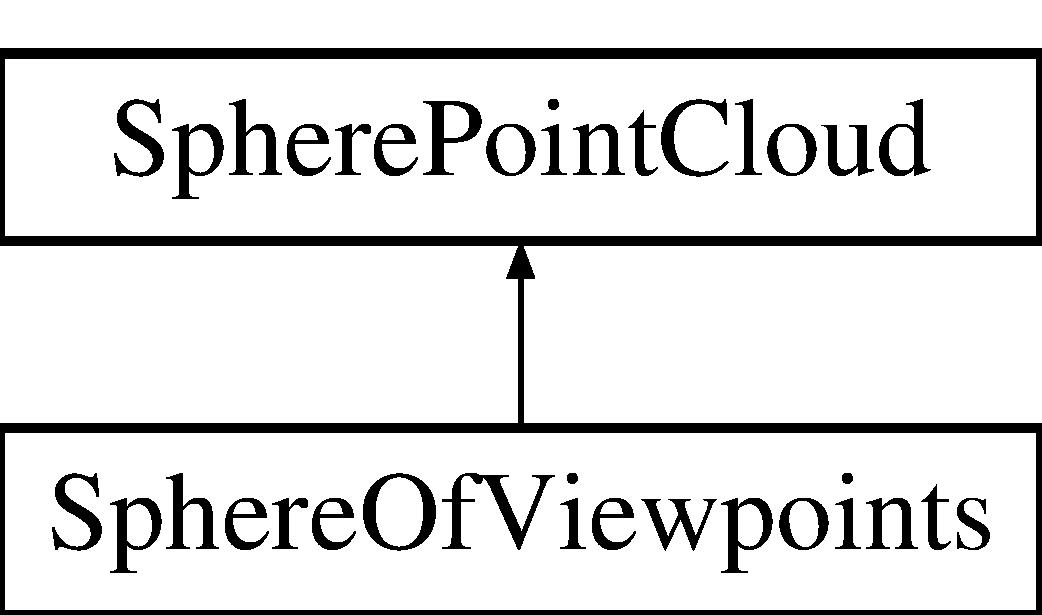
\includegraphics[height=2.000000cm]{class_sphere_point_cloud}
\end{center}
\end{figure}
\subsection*{Public Member Functions}
\begin{DoxyCompactItemize}
\item 
\hyperlink{class_sphere_point_cloud_a2b7e0b5989a455ec7986d9d536f3ce21}{Sphere\+Point\+Cloud} ()
\begin{DoxyCompactList}\small\item\em Constructor. \end{DoxyCompactList}\item 
\hyperlink{class_sphere_point_cloud_ac1d6c155589d2a2c5e1344461237370e}{Sphere\+Point\+Cloud} (const \hyperlink{class_sphere_point_cloud}{Sphere\+Point\+Cloud} \&p\+Sphere\+Point\+Cloud)
\begin{DoxyCompactList}\small\item\em Copy constructor. \end{DoxyCompactList}\item 
\hyperlink{class_sphere_point_cloud_a0257f3ce5bdc5ddd24bbb49c21d8a9f5}{$\sim$\+Sphere\+Point\+Cloud} ()
\begin{DoxyCompactList}\small\item\em Destructor. \end{DoxyCompactList}\item 
void \hyperlink{class_sphere_point_cloud_a2653050cf6623de85dc67427b3a4145f}{Set\+To\+Uniform4} ()
\begin{DoxyCompactList}\small\item\em Generates 4 points uniformly distributed. \end{DoxyCompactList}\item 
void \hyperlink{class_sphere_point_cloud_a3ec027baeb8148420e9429beeb0f9083}{Set\+To\+Uniform6} ()
\begin{DoxyCompactList}\small\item\em Generates 6 points uniformly distributed. \end{DoxyCompactList}\item 
void \hyperlink{class_sphere_point_cloud_accc06313864eaa198971ef0108bcb3ca}{Set\+To\+Uniform8} ()
\begin{DoxyCompactList}\small\item\em Generates 8 points uniformly distributed. \end{DoxyCompactList}\item 
void \hyperlink{class_sphere_point_cloud_a91f91589cc74911158165b6adf46b428}{Set\+To\+Uniform12} ()
\begin{DoxyCompactList}\small\item\em Generates 12 points uniformly distributed. \end{DoxyCompactList}\item 
void \hyperlink{class_sphere_point_cloud_a22f25a4447052eb8c98dea4ace790c8b}{Set\+To\+Uniform20} ()
\begin{DoxyCompactList}\small\item\em Generates 20 points uniformly distributed. \end{DoxyCompactList}\item 
void \hyperlink{class_sphere_point_cloud_a1eff636a5b32f0951a33a9cf7598c1d9}{Set\+To\+Quasi\+Uniform} (unsigned char p\+Depth)
\item 
Q\+Vector$<$ unsigned int $>$ \hyperlink{class_sphere_point_cloud_a381347a4f912ecc8d2012086324e0d56}{Get\+Faces} () const 
\begin{DoxyCompactList}\small\item\em Return the faces of the triangles. \end{DoxyCompactList}\item 
Q\+Vector$<$ glm\+::vec3 $>$ \hyperlink{class_sphere_point_cloud_aa3cd921f38a53c64d3fb4833860fbd9c}{Get\+Vertices} () const 
\begin{DoxyCompactList}\small\item\em Return the points in cartesian coordinates. \end{DoxyCompactList}\item 
glm\+::vec3 \hyperlink{class_sphere_point_cloud_a4e076465c1f7f26970794e4c0f8e8adb}{Get\+Vertex} (unsigned int p\+I) const 
\begin{DoxyCompactList}\small\item\em Return the vertex {\itshape p\+I}. \end{DoxyCompactList}\item 
Q\+Vector$<$ Q\+Vector$<$ int $>$ $>$ \hyperlink{class_sphere_point_cloud_a0004a4d225831127eaafaa28dc13b416}{Get\+Neighbours} () const 
\begin{DoxyCompactList}\small\item\em Return the neighbours of every point. \end{DoxyCompactList}\item 
Q\+Vector$<$ int $>$ \hyperlink{class_sphere_point_cloud_ac83eb3eac8c51a2bbec28ff2a40a985c}{Get\+Neighbours} (unsigned int p\+I) const 
\begin{DoxyCompactList}\small\item\em Return the neighbours of the point {\itshape p\+I}. \end{DoxyCompactList}\item 
\hyperlink{class_geometry}{Geometry} $\ast$ \hyperlink{class_sphere_point_cloud_afb0abeffb85e483961fd08a7e58e3440}{Get\+Mesh} () const 
\begin{DoxyCompactList}\small\item\em Return the 3\+D mesh. \end{DoxyCompactList}\end{DoxyCompactItemize}
\subsection*{Static Public Member Functions}
\begin{DoxyCompactItemize}
\item 
static glm\+::vec3 \hyperlink{class_sphere_point_cloud_a2182e6f3e31bb91347a4b3d15cf3ebbe}{Up} (const glm\+::vec3 \&p\+Viewpoint)
\begin{DoxyCompactList}\small\item\em Retorna un vector cap amunt per al punt de vista passat. \end{DoxyCompactList}\end{DoxyCompactItemize}
\subsection*{Protected Member Functions}
\begin{DoxyCompactItemize}
\item 
void \hyperlink{class_sphere_point_cloud_a01bf0317e5a3b1229bdafc9f4ff92c37}{Set\+Mesh\+Information} ()
\begin{DoxyCompactList}\small\item\em Configure the mesh. \end{DoxyCompactList}\end{DoxyCompactItemize}
\subsection*{Protected Attributes}
\begin{DoxyCompactItemize}
\item 
\hyperlink{class_geometry}{Geometry} $\ast$ \hyperlink{class_sphere_point_cloud_a722ae327d20905a422c279bc0bc60258}{m\+Mesh}
\begin{DoxyCompactList}\small\item\em \hyperlink{class_mesh}{Mesh} to paint the sphere point cloud. \end{DoxyCompactList}\item 
int \hyperlink{class_sphere_point_cloud_a0579096387a36228a7167de55d131292}{m\+Number\+Of\+Points}
\begin{DoxyCompactList}\small\item\em Number of points. \end{DoxyCompactList}\item 
Q\+Vector$<$ unsigned int $>$ \hyperlink{class_sphere_point_cloud_a1493117ae52c168b3ca2dc0a395faf65}{m\+Faces}
\begin{DoxyCompactList}\small\item\em Faces. \end{DoxyCompactList}\item 
Q\+Vector$<$ glm\+::vec3 $>$ \hyperlink{class_sphere_point_cloud_a03bccf235a21adebdfcd6a8e4c407c72}{m\+Vertices}
\begin{DoxyCompactList}\small\item\em Vertexs in cartesian coordinates. \end{DoxyCompactList}\item 
Q\+Vector$<$ glm\+::vec3 $>$ \hyperlink{class_sphere_point_cloud_a01a10f53b2432af26235a1acc98391eb}{m\+Normals}
\begin{DoxyCompactList}\small\item\em Normals of the vertexs. \end{DoxyCompactList}\item 
Q\+Vector$<$ Q\+Vector$<$ int $>$ $>$ \hyperlink{class_sphere_point_cloud_a11b1736edb303b804dc0882edc8718a8}{m\+Neighbours}
\begin{DoxyCompactList}\small\item\em Neighbours of the vertexs. \end{DoxyCompactList}\end{DoxyCompactItemize}
\subsection*{Private Member Functions}
\begin{DoxyCompactItemize}
\item 
void \hyperlink{class_sphere_point_cloud_a3e0d3c60d70cfe99c2d6de29c73c03da}{Compute\+Quasi\+Uniform\+Neighbours} ()
\begin{DoxyCompactList}\small\item\em Compute the neighbours of the quasi uniform distribution. \end{DoxyCompactList}\item 
void \hyperlink{class_sphere_point_cloud_a2b3f0d6a9ec362b7092d5d57db48a308}{Create\+Icosahedron} ()
\begin{DoxyCompactList}\small\item\em Create the vertexs, faces and normals of an icosahedron (level 0) \end{DoxyCompactList}\item 
bool \hyperlink{class_sphere_point_cloud_aa3b15e437f2985aba5cc4d25f6247f31}{Find\+Sphere\+Cloud\+Vertex} (const glm\+::vec3 \&p\+V, unsigned int \&p\+Position) const 
\begin{DoxyCompactList}\small\item\em Find if a vertex already exists, if exists return the index. \end{DoxyCompactList}\item 
void \hyperlink{class_sphere_point_cloud_acbdfea7e32eb80be3f7f789a341aaee4}{Create\+Sphere\+Cloud\+Triangle} (const glm\+::vec3 \&p\+V1, const glm\+::vec3 \&p\+V2, const glm\+::vec3 \&p\+V3)
\begin{DoxyCompactList}\small\item\em Create a new face with 3 vertex from the point cloud. \end{DoxyCompactList}\item 
void \hyperlink{class_sphere_point_cloud_ac6da28fe26729163facc32139595e758}{Subdivide} (glm\+::vec3 p\+V1, glm\+::vec3 p\+V2, glm\+::vec3 p\+V3, unsigned short p\+Depth)
\begin{DoxyCompactList}\small\item\em Subdivide the point cloud recursively until {\itshape p\+Depth}. \end{DoxyCompactList}\end{DoxyCompactItemize}


\subsection{Detailed Description}
Sphere of points uniformly or quasi-\/uniformly distributed

\begin{DoxyAuthor}{Author}
Francisco González 

Marc Ruiz 

Xavier Bonaventura 

Copyright\+: (c) Universitat de Girona 
\end{DoxyAuthor}


\subsection{Constructor \& Destructor Documentation}
\hypertarget{class_sphere_point_cloud_a2b7e0b5989a455ec7986d9d536f3ce21}{\index{Sphere\+Point\+Cloud@{Sphere\+Point\+Cloud}!Sphere\+Point\+Cloud@{Sphere\+Point\+Cloud}}
\index{Sphere\+Point\+Cloud@{Sphere\+Point\+Cloud}!Sphere\+Point\+Cloud@{Sphere\+Point\+Cloud}}
\subsubsection[{Sphere\+Point\+Cloud}]{\setlength{\rightskip}{0pt plus 5cm}Sphere\+Point\+Cloud\+::\+Sphere\+Point\+Cloud (
\begin{DoxyParamCaption}
{}
\end{DoxyParamCaption}
)}}\label{class_sphere_point_cloud_a2b7e0b5989a455ec7986d9d536f3ce21}


Constructor. 

\hypertarget{class_sphere_point_cloud_ac1d6c155589d2a2c5e1344461237370e}{\index{Sphere\+Point\+Cloud@{Sphere\+Point\+Cloud}!Sphere\+Point\+Cloud@{Sphere\+Point\+Cloud}}
\index{Sphere\+Point\+Cloud@{Sphere\+Point\+Cloud}!Sphere\+Point\+Cloud@{Sphere\+Point\+Cloud}}
\subsubsection[{Sphere\+Point\+Cloud}]{\setlength{\rightskip}{0pt plus 5cm}Sphere\+Point\+Cloud\+::\+Sphere\+Point\+Cloud (
\begin{DoxyParamCaption}
\item[{const {\bf Sphere\+Point\+Cloud} \&}]{p\+Sphere\+Point\+Cloud}
\end{DoxyParamCaption}
)}}\label{class_sphere_point_cloud_ac1d6c155589d2a2c5e1344461237370e}


Copy constructor. 

\hypertarget{class_sphere_point_cloud_a0257f3ce5bdc5ddd24bbb49c21d8a9f5}{\index{Sphere\+Point\+Cloud@{Sphere\+Point\+Cloud}!````~Sphere\+Point\+Cloud@{$\sim$\+Sphere\+Point\+Cloud}}
\index{````~Sphere\+Point\+Cloud@{$\sim$\+Sphere\+Point\+Cloud}!Sphere\+Point\+Cloud@{Sphere\+Point\+Cloud}}
\subsubsection[{$\sim$\+Sphere\+Point\+Cloud}]{\setlength{\rightskip}{0pt plus 5cm}Sphere\+Point\+Cloud\+::$\sim$\+Sphere\+Point\+Cloud (
\begin{DoxyParamCaption}
{}
\end{DoxyParamCaption}
)}}\label{class_sphere_point_cloud_a0257f3ce5bdc5ddd24bbb49c21d8a9f5}


Destructor. 



\subsection{Member Function Documentation}
\hypertarget{class_sphere_point_cloud_a3e0d3c60d70cfe99c2d6de29c73c03da}{\index{Sphere\+Point\+Cloud@{Sphere\+Point\+Cloud}!Compute\+Quasi\+Uniform\+Neighbours@{Compute\+Quasi\+Uniform\+Neighbours}}
\index{Compute\+Quasi\+Uniform\+Neighbours@{Compute\+Quasi\+Uniform\+Neighbours}!Sphere\+Point\+Cloud@{Sphere\+Point\+Cloud}}
\subsubsection[{Compute\+Quasi\+Uniform\+Neighbours}]{\setlength{\rightskip}{0pt plus 5cm}void Sphere\+Point\+Cloud\+::\+Compute\+Quasi\+Uniform\+Neighbours (
\begin{DoxyParamCaption}
{}
\end{DoxyParamCaption}
)\hspace{0.3cm}{\ttfamily [private]}}}\label{class_sphere_point_cloud_a3e0d3c60d70cfe99c2d6de29c73c03da}


Compute the neighbours of the quasi uniform distribution. 

\hypertarget{class_sphere_point_cloud_a2b3f0d6a9ec362b7092d5d57db48a308}{\index{Sphere\+Point\+Cloud@{Sphere\+Point\+Cloud}!Create\+Icosahedron@{Create\+Icosahedron}}
\index{Create\+Icosahedron@{Create\+Icosahedron}!Sphere\+Point\+Cloud@{Sphere\+Point\+Cloud}}
\subsubsection[{Create\+Icosahedron}]{\setlength{\rightskip}{0pt plus 5cm}void Sphere\+Point\+Cloud\+::\+Create\+Icosahedron (
\begin{DoxyParamCaption}
{}
\end{DoxyParamCaption}
)\hspace{0.3cm}{\ttfamily [private]}}}\label{class_sphere_point_cloud_a2b3f0d6a9ec362b7092d5d57db48a308}


Create the vertexs, faces and normals of an icosahedron (level 0) 

\hypertarget{class_sphere_point_cloud_acbdfea7e32eb80be3f7f789a341aaee4}{\index{Sphere\+Point\+Cloud@{Sphere\+Point\+Cloud}!Create\+Sphere\+Cloud\+Triangle@{Create\+Sphere\+Cloud\+Triangle}}
\index{Create\+Sphere\+Cloud\+Triangle@{Create\+Sphere\+Cloud\+Triangle}!Sphere\+Point\+Cloud@{Sphere\+Point\+Cloud}}
\subsubsection[{Create\+Sphere\+Cloud\+Triangle}]{\setlength{\rightskip}{0pt plus 5cm}void Sphere\+Point\+Cloud\+::\+Create\+Sphere\+Cloud\+Triangle (
\begin{DoxyParamCaption}
\item[{const glm\+::vec3 \&}]{p\+V1, }
\item[{const glm\+::vec3 \&}]{p\+V2, }
\item[{const glm\+::vec3 \&}]{p\+V3}
\end{DoxyParamCaption}
)\hspace{0.3cm}{\ttfamily [private]}}}\label{class_sphere_point_cloud_acbdfea7e32eb80be3f7f789a341aaee4}


Create a new face with 3 vertex from the point cloud. 

\hypertarget{class_sphere_point_cloud_aa3b15e437f2985aba5cc4d25f6247f31}{\index{Sphere\+Point\+Cloud@{Sphere\+Point\+Cloud}!Find\+Sphere\+Cloud\+Vertex@{Find\+Sphere\+Cloud\+Vertex}}
\index{Find\+Sphere\+Cloud\+Vertex@{Find\+Sphere\+Cloud\+Vertex}!Sphere\+Point\+Cloud@{Sphere\+Point\+Cloud}}
\subsubsection[{Find\+Sphere\+Cloud\+Vertex}]{\setlength{\rightskip}{0pt plus 5cm}bool Sphere\+Point\+Cloud\+::\+Find\+Sphere\+Cloud\+Vertex (
\begin{DoxyParamCaption}
\item[{const glm\+::vec3 \&}]{p\+V, }
\item[{unsigned int \&}]{p\+Position}
\end{DoxyParamCaption}
) const\hspace{0.3cm}{\ttfamily [private]}}}\label{class_sphere_point_cloud_aa3b15e437f2985aba5cc4d25f6247f31}


Find if a vertex already exists, if exists return the index. 

\hypertarget{class_sphere_point_cloud_a381347a4f912ecc8d2012086324e0d56}{\index{Sphere\+Point\+Cloud@{Sphere\+Point\+Cloud}!Get\+Faces@{Get\+Faces}}
\index{Get\+Faces@{Get\+Faces}!Sphere\+Point\+Cloud@{Sphere\+Point\+Cloud}}
\subsubsection[{Get\+Faces}]{\setlength{\rightskip}{0pt plus 5cm}Q\+Vector$<$ unsigned int $>$ Sphere\+Point\+Cloud\+::\+Get\+Faces (
\begin{DoxyParamCaption}
{}
\end{DoxyParamCaption}
) const}}\label{class_sphere_point_cloud_a381347a4f912ecc8d2012086324e0d56}


Return the faces of the triangles. 

\hypertarget{class_sphere_point_cloud_afb0abeffb85e483961fd08a7e58e3440}{\index{Sphere\+Point\+Cloud@{Sphere\+Point\+Cloud}!Get\+Mesh@{Get\+Mesh}}
\index{Get\+Mesh@{Get\+Mesh}!Sphere\+Point\+Cloud@{Sphere\+Point\+Cloud}}
\subsubsection[{Get\+Mesh}]{\setlength{\rightskip}{0pt plus 5cm}{\bf Geometry} $\ast$ Sphere\+Point\+Cloud\+::\+Get\+Mesh (
\begin{DoxyParamCaption}
{}
\end{DoxyParamCaption}
) const}}\label{class_sphere_point_cloud_afb0abeffb85e483961fd08a7e58e3440}


Return the 3\+D mesh. 

\hypertarget{class_sphere_point_cloud_a0004a4d225831127eaafaa28dc13b416}{\index{Sphere\+Point\+Cloud@{Sphere\+Point\+Cloud}!Get\+Neighbours@{Get\+Neighbours}}
\index{Get\+Neighbours@{Get\+Neighbours}!Sphere\+Point\+Cloud@{Sphere\+Point\+Cloud}}
\subsubsection[{Get\+Neighbours}]{\setlength{\rightskip}{0pt plus 5cm}Q\+Vector$<$ Q\+Vector$<$ int $>$ $>$ Sphere\+Point\+Cloud\+::\+Get\+Neighbours (
\begin{DoxyParamCaption}
{}
\end{DoxyParamCaption}
) const}}\label{class_sphere_point_cloud_a0004a4d225831127eaafaa28dc13b416}


Return the neighbours of every point. 

\hypertarget{class_sphere_point_cloud_ac83eb3eac8c51a2bbec28ff2a40a985c}{\index{Sphere\+Point\+Cloud@{Sphere\+Point\+Cloud}!Get\+Neighbours@{Get\+Neighbours}}
\index{Get\+Neighbours@{Get\+Neighbours}!Sphere\+Point\+Cloud@{Sphere\+Point\+Cloud}}
\subsubsection[{Get\+Neighbours}]{\setlength{\rightskip}{0pt plus 5cm}Q\+Vector$<$ int $>$ Sphere\+Point\+Cloud\+::\+Get\+Neighbours (
\begin{DoxyParamCaption}
\item[{unsigned int}]{p\+I}
\end{DoxyParamCaption}
) const}}\label{class_sphere_point_cloud_ac83eb3eac8c51a2bbec28ff2a40a985c}


Return the neighbours of the point {\itshape p\+I}. 

\hypertarget{class_sphere_point_cloud_a4e076465c1f7f26970794e4c0f8e8adb}{\index{Sphere\+Point\+Cloud@{Sphere\+Point\+Cloud}!Get\+Vertex@{Get\+Vertex}}
\index{Get\+Vertex@{Get\+Vertex}!Sphere\+Point\+Cloud@{Sphere\+Point\+Cloud}}
\subsubsection[{Get\+Vertex}]{\setlength{\rightskip}{0pt plus 5cm}glm\+::vec3 Sphere\+Point\+Cloud\+::\+Get\+Vertex (
\begin{DoxyParamCaption}
\item[{unsigned int}]{p\+I}
\end{DoxyParamCaption}
) const}}\label{class_sphere_point_cloud_a4e076465c1f7f26970794e4c0f8e8adb}


Return the vertex {\itshape p\+I}. 

\hypertarget{class_sphere_point_cloud_aa3cd921f38a53c64d3fb4833860fbd9c}{\index{Sphere\+Point\+Cloud@{Sphere\+Point\+Cloud}!Get\+Vertices@{Get\+Vertices}}
\index{Get\+Vertices@{Get\+Vertices}!Sphere\+Point\+Cloud@{Sphere\+Point\+Cloud}}
\subsubsection[{Get\+Vertices}]{\setlength{\rightskip}{0pt plus 5cm}Q\+Vector$<$ glm\+::vec3 $>$ Sphere\+Point\+Cloud\+::\+Get\+Vertices (
\begin{DoxyParamCaption}
{}
\end{DoxyParamCaption}
) const}}\label{class_sphere_point_cloud_aa3cd921f38a53c64d3fb4833860fbd9c}


Return the points in cartesian coordinates. 

\hypertarget{class_sphere_point_cloud_a01bf0317e5a3b1229bdafc9f4ff92c37}{\index{Sphere\+Point\+Cloud@{Sphere\+Point\+Cloud}!Set\+Mesh\+Information@{Set\+Mesh\+Information}}
\index{Set\+Mesh\+Information@{Set\+Mesh\+Information}!Sphere\+Point\+Cloud@{Sphere\+Point\+Cloud}}
\subsubsection[{Set\+Mesh\+Information}]{\setlength{\rightskip}{0pt plus 5cm}void Sphere\+Point\+Cloud\+::\+Set\+Mesh\+Information (
\begin{DoxyParamCaption}
{}
\end{DoxyParamCaption}
)\hspace{0.3cm}{\ttfamily [protected]}}}\label{class_sphere_point_cloud_a01bf0317e5a3b1229bdafc9f4ff92c37}


Configure the mesh. 

\hypertarget{class_sphere_point_cloud_a1eff636a5b32f0951a33a9cf7598c1d9}{\index{Sphere\+Point\+Cloud@{Sphere\+Point\+Cloud}!Set\+To\+Quasi\+Uniform@{Set\+To\+Quasi\+Uniform}}
\index{Set\+To\+Quasi\+Uniform@{Set\+To\+Quasi\+Uniform}!Sphere\+Point\+Cloud@{Sphere\+Point\+Cloud}}
\subsubsection[{Set\+To\+Quasi\+Uniform}]{\setlength{\rightskip}{0pt plus 5cm}void Sphere\+Point\+Cloud\+::\+Set\+To\+Quasi\+Uniform (
\begin{DoxyParamCaption}
\item[{unsigned char}]{p\+Depth}
\end{DoxyParamCaption}
)}}\label{class_sphere_point_cloud_a1eff636a5b32f0951a33a9cf7598c1d9}
Generate 10$\ast$4$^\wedge$depth+2 points quasi-\/uniformly distributed using the recursive subdivision of faces, starting from an icosahedron \hypertarget{class_sphere_point_cloud_a91f91589cc74911158165b6adf46b428}{\index{Sphere\+Point\+Cloud@{Sphere\+Point\+Cloud}!Set\+To\+Uniform12@{Set\+To\+Uniform12}}
\index{Set\+To\+Uniform12@{Set\+To\+Uniform12}!Sphere\+Point\+Cloud@{Sphere\+Point\+Cloud}}
\subsubsection[{Set\+To\+Uniform12}]{\setlength{\rightskip}{0pt plus 5cm}void Sphere\+Point\+Cloud\+::\+Set\+To\+Uniform12 (
\begin{DoxyParamCaption}
{}
\end{DoxyParamCaption}
)}}\label{class_sphere_point_cloud_a91f91589cc74911158165b6adf46b428}


Generates 12 points uniformly distributed. 

\hypertarget{class_sphere_point_cloud_a22f25a4447052eb8c98dea4ace790c8b}{\index{Sphere\+Point\+Cloud@{Sphere\+Point\+Cloud}!Set\+To\+Uniform20@{Set\+To\+Uniform20}}
\index{Set\+To\+Uniform20@{Set\+To\+Uniform20}!Sphere\+Point\+Cloud@{Sphere\+Point\+Cloud}}
\subsubsection[{Set\+To\+Uniform20}]{\setlength{\rightskip}{0pt plus 5cm}void Sphere\+Point\+Cloud\+::\+Set\+To\+Uniform20 (
\begin{DoxyParamCaption}
{}
\end{DoxyParamCaption}
)}}\label{class_sphere_point_cloud_a22f25a4447052eb8c98dea4ace790c8b}


Generates 20 points uniformly distributed. 

\hypertarget{class_sphere_point_cloud_a2653050cf6623de85dc67427b3a4145f}{\index{Sphere\+Point\+Cloud@{Sphere\+Point\+Cloud}!Set\+To\+Uniform4@{Set\+To\+Uniform4}}
\index{Set\+To\+Uniform4@{Set\+To\+Uniform4}!Sphere\+Point\+Cloud@{Sphere\+Point\+Cloud}}
\subsubsection[{Set\+To\+Uniform4}]{\setlength{\rightskip}{0pt plus 5cm}void Sphere\+Point\+Cloud\+::\+Set\+To\+Uniform4 (
\begin{DoxyParamCaption}
{}
\end{DoxyParamCaption}
)}}\label{class_sphere_point_cloud_a2653050cf6623de85dc67427b3a4145f}


Generates 4 points uniformly distributed. 

\hypertarget{class_sphere_point_cloud_a3ec027baeb8148420e9429beeb0f9083}{\index{Sphere\+Point\+Cloud@{Sphere\+Point\+Cloud}!Set\+To\+Uniform6@{Set\+To\+Uniform6}}
\index{Set\+To\+Uniform6@{Set\+To\+Uniform6}!Sphere\+Point\+Cloud@{Sphere\+Point\+Cloud}}
\subsubsection[{Set\+To\+Uniform6}]{\setlength{\rightskip}{0pt plus 5cm}void Sphere\+Point\+Cloud\+::\+Set\+To\+Uniform6 (
\begin{DoxyParamCaption}
{}
\end{DoxyParamCaption}
)}}\label{class_sphere_point_cloud_a3ec027baeb8148420e9429beeb0f9083}


Generates 6 points uniformly distributed. 

\hypertarget{class_sphere_point_cloud_accc06313864eaa198971ef0108bcb3ca}{\index{Sphere\+Point\+Cloud@{Sphere\+Point\+Cloud}!Set\+To\+Uniform8@{Set\+To\+Uniform8}}
\index{Set\+To\+Uniform8@{Set\+To\+Uniform8}!Sphere\+Point\+Cloud@{Sphere\+Point\+Cloud}}
\subsubsection[{Set\+To\+Uniform8}]{\setlength{\rightskip}{0pt plus 5cm}void Sphere\+Point\+Cloud\+::\+Set\+To\+Uniform8 (
\begin{DoxyParamCaption}
{}
\end{DoxyParamCaption}
)}}\label{class_sphere_point_cloud_accc06313864eaa198971ef0108bcb3ca}


Generates 8 points uniformly distributed. 

\hypertarget{class_sphere_point_cloud_ac6da28fe26729163facc32139595e758}{\index{Sphere\+Point\+Cloud@{Sphere\+Point\+Cloud}!Subdivide@{Subdivide}}
\index{Subdivide@{Subdivide}!Sphere\+Point\+Cloud@{Sphere\+Point\+Cloud}}
\subsubsection[{Subdivide}]{\setlength{\rightskip}{0pt plus 5cm}void Sphere\+Point\+Cloud\+::\+Subdivide (
\begin{DoxyParamCaption}
\item[{glm\+::vec3}]{p\+V1, }
\item[{glm\+::vec3}]{p\+V2, }
\item[{glm\+::vec3}]{p\+V3, }
\item[{unsigned short}]{p\+Depth}
\end{DoxyParamCaption}
)\hspace{0.3cm}{\ttfamily [private]}}}\label{class_sphere_point_cloud_ac6da28fe26729163facc32139595e758}


Subdivide the point cloud recursively until {\itshape p\+Depth}. 

\hypertarget{class_sphere_point_cloud_a2182e6f3e31bb91347a4b3d15cf3ebbe}{\index{Sphere\+Point\+Cloud@{Sphere\+Point\+Cloud}!Up@{Up}}
\index{Up@{Up}!Sphere\+Point\+Cloud@{Sphere\+Point\+Cloud}}
\subsubsection[{Up}]{\setlength{\rightskip}{0pt plus 5cm}glm\+::vec3 Sphere\+Point\+Cloud\+::\+Up (
\begin{DoxyParamCaption}
\item[{const glm\+::vec3 \&}]{p\+Viewpoint}
\end{DoxyParamCaption}
)\hspace{0.3cm}{\ttfamily [static]}}}\label{class_sphere_point_cloud_a2182e6f3e31bb91347a4b3d15cf3ebbe}


Retorna un vector cap amunt per al punt de vista passat. 



\subsection{Member Data Documentation}
\hypertarget{class_sphere_point_cloud_a1493117ae52c168b3ca2dc0a395faf65}{\index{Sphere\+Point\+Cloud@{Sphere\+Point\+Cloud}!m\+Faces@{m\+Faces}}
\index{m\+Faces@{m\+Faces}!Sphere\+Point\+Cloud@{Sphere\+Point\+Cloud}}
\subsubsection[{m\+Faces}]{\setlength{\rightskip}{0pt plus 5cm}Q\+Vector$<$ unsigned int $>$ Sphere\+Point\+Cloud\+::m\+Faces\hspace{0.3cm}{\ttfamily [protected]}}}\label{class_sphere_point_cloud_a1493117ae52c168b3ca2dc0a395faf65}


Faces. 

\hypertarget{class_sphere_point_cloud_a722ae327d20905a422c279bc0bc60258}{\index{Sphere\+Point\+Cloud@{Sphere\+Point\+Cloud}!m\+Mesh@{m\+Mesh}}
\index{m\+Mesh@{m\+Mesh}!Sphere\+Point\+Cloud@{Sphere\+Point\+Cloud}}
\subsubsection[{m\+Mesh}]{\setlength{\rightskip}{0pt plus 5cm}{\bf Geometry}$\ast$ Sphere\+Point\+Cloud\+::m\+Mesh\hspace{0.3cm}{\ttfamily [protected]}}}\label{class_sphere_point_cloud_a722ae327d20905a422c279bc0bc60258}


\hyperlink{class_mesh}{Mesh} to paint the sphere point cloud. 

\hypertarget{class_sphere_point_cloud_a11b1736edb303b804dc0882edc8718a8}{\index{Sphere\+Point\+Cloud@{Sphere\+Point\+Cloud}!m\+Neighbours@{m\+Neighbours}}
\index{m\+Neighbours@{m\+Neighbours}!Sphere\+Point\+Cloud@{Sphere\+Point\+Cloud}}
\subsubsection[{m\+Neighbours}]{\setlength{\rightskip}{0pt plus 5cm}Q\+Vector$<$ Q\+Vector$<$int$>$ $>$ Sphere\+Point\+Cloud\+::m\+Neighbours\hspace{0.3cm}{\ttfamily [protected]}}}\label{class_sphere_point_cloud_a11b1736edb303b804dc0882edc8718a8}


Neighbours of the vertexs. 

\hypertarget{class_sphere_point_cloud_a01a10f53b2432af26235a1acc98391eb}{\index{Sphere\+Point\+Cloud@{Sphere\+Point\+Cloud}!m\+Normals@{m\+Normals}}
\index{m\+Normals@{m\+Normals}!Sphere\+Point\+Cloud@{Sphere\+Point\+Cloud}}
\subsubsection[{m\+Normals}]{\setlength{\rightskip}{0pt plus 5cm}Q\+Vector$<$ glm\+::vec3 $>$ Sphere\+Point\+Cloud\+::m\+Normals\hspace{0.3cm}{\ttfamily [protected]}}}\label{class_sphere_point_cloud_a01a10f53b2432af26235a1acc98391eb}


Normals of the vertexs. 

\hypertarget{class_sphere_point_cloud_a0579096387a36228a7167de55d131292}{\index{Sphere\+Point\+Cloud@{Sphere\+Point\+Cloud}!m\+Number\+Of\+Points@{m\+Number\+Of\+Points}}
\index{m\+Number\+Of\+Points@{m\+Number\+Of\+Points}!Sphere\+Point\+Cloud@{Sphere\+Point\+Cloud}}
\subsubsection[{m\+Number\+Of\+Points}]{\setlength{\rightskip}{0pt plus 5cm}int Sphere\+Point\+Cloud\+::m\+Number\+Of\+Points\hspace{0.3cm}{\ttfamily [protected]}}}\label{class_sphere_point_cloud_a0579096387a36228a7167de55d131292}


Number of points. 

\hypertarget{class_sphere_point_cloud_a03bccf235a21adebdfcd6a8e4c407c72}{\index{Sphere\+Point\+Cloud@{Sphere\+Point\+Cloud}!m\+Vertices@{m\+Vertices}}
\index{m\+Vertices@{m\+Vertices}!Sphere\+Point\+Cloud@{Sphere\+Point\+Cloud}}
\subsubsection[{m\+Vertices}]{\setlength{\rightskip}{0pt plus 5cm}Q\+Vector$<$ glm\+::vec3 $>$ Sphere\+Point\+Cloud\+::m\+Vertices\hspace{0.3cm}{\ttfamily [protected]}}}\label{class_sphere_point_cloud_a03bccf235a21adebdfcd6a8e4c407c72}


Vertexs in cartesian coordinates. 



The documentation for this class was generated from the following files\+:\begin{DoxyCompactItemize}
\item 
inc/\hyperlink{_sphere_point_cloud_8h}{Sphere\+Point\+Cloud.\+h}\item 
src/\hyperlink{_sphere_point_cloud_8cpp}{Sphere\+Point\+Cloud.\+cpp}\end{DoxyCompactItemize}

\hypertarget{class_stoev_strasser}{\section{Stoev\+Strasser Class Reference}
\label{class_stoev_strasser}\index{Stoev\+Strasser@{Stoev\+Strasser}}
}


Class that implements the Stoev and Strasser measure \mbox{[}Stoev and Strasser 2002\mbox{]}.  




{\ttfamily \#include $<$Stoev\+Strasser.\+h$>$}

Inheritance diagram for Stoev\+Strasser\+:\begin{figure}[H]
\begin{center}
\leavevmode
\includegraphics[height=2.000000cm]{class_stoev_strasser}
\end{center}
\end{figure}
\subsection*{Public Member Functions}
\begin{DoxyCompactItemize}
\item 
\hyperlink{class_stoev_strasser_aa671f75420b0c973d311a4d96c625db8}{Stoev\+Strasser} (const Q\+String \&p\+Name)
\begin{DoxyCompactList}\small\item\em Constructor. \end{DoxyCompactList}\item 
\hyperlink{class_stoev_strasser_aeb82ff6ec419b248c922575dded53dad}{$\sim$\+Stoev\+Strasser} ()
\begin{DoxyCompactList}\small\item\em Destructor. \end{DoxyCompactList}\item 
void \hyperlink{class_stoev_strasser_ad30bd5fd1ada91b99235297aba1e4517}{Compute} (const \hyperlink{class_scene_information_builder}{Scene\+Information\+Builder} $\ast$p\+Scene\+Information\+Builder)
\begin{DoxyCompactList}\small\item\em Method that computes the measure. \end{DoxyCompactList}\end{DoxyCompactItemize}
\subsection*{Additional Inherited Members}


\subsection{Detailed Description}
Class that implements the Stoev and Strasser measure \mbox{[}Stoev and Strasser 2002\mbox{]}. 

\begin{DoxyAuthor}{Author}
Xavier Bonaventura 

Copyright\+: (c) Universitat de Girona 
\end{DoxyAuthor}


\subsection{Constructor \& Destructor Documentation}
\hypertarget{class_stoev_strasser_aa671f75420b0c973d311a4d96c625db8}{\index{Stoev\+Strasser@{Stoev\+Strasser}!Stoev\+Strasser@{Stoev\+Strasser}}
\index{Stoev\+Strasser@{Stoev\+Strasser}!Stoev\+Strasser@{Stoev\+Strasser}}
\subsubsection[{Stoev\+Strasser}]{\setlength{\rightskip}{0pt plus 5cm}Stoev\+Strasser\+::\+Stoev\+Strasser (
\begin{DoxyParamCaption}
\item[{const Q\+String \&}]{p\+Name}
\end{DoxyParamCaption}
)}}\label{class_stoev_strasser_aa671f75420b0c973d311a4d96c625db8}


Constructor. 

\hypertarget{class_stoev_strasser_aeb82ff6ec419b248c922575dded53dad}{\index{Stoev\+Strasser@{Stoev\+Strasser}!````~Stoev\+Strasser@{$\sim$\+Stoev\+Strasser}}
\index{````~Stoev\+Strasser@{$\sim$\+Stoev\+Strasser}!Stoev\+Strasser@{Stoev\+Strasser}}
\subsubsection[{$\sim$\+Stoev\+Strasser}]{\setlength{\rightskip}{0pt plus 5cm}Stoev\+Strasser\+::$\sim$\+Stoev\+Strasser (
\begin{DoxyParamCaption}
{}
\end{DoxyParamCaption}
)}}\label{class_stoev_strasser_aeb82ff6ec419b248c922575dded53dad}


Destructor. 



\subsection{Member Function Documentation}
\hypertarget{class_stoev_strasser_ad30bd5fd1ada91b99235297aba1e4517}{\index{Stoev\+Strasser@{Stoev\+Strasser}!Compute@{Compute}}
\index{Compute@{Compute}!Stoev\+Strasser@{Stoev\+Strasser}}
\subsubsection[{Compute}]{\setlength{\rightskip}{0pt plus 5cm}void Stoev\+Strasser\+::\+Compute (
\begin{DoxyParamCaption}
\item[{const {\bf Scene\+Information\+Builder} $\ast$}]{p\+Scene\+Information\+Builder}
\end{DoxyParamCaption}
)\hspace{0.3cm}{\ttfamily [virtual]}}}\label{class_stoev_strasser_ad30bd5fd1ada91b99235297aba1e4517}


Method that computes the measure. 



Implements \hyperlink{class_measure_aed88fe46b2a609ab5948e5f3c891321d}{Measure}.



The documentation for this class was generated from the following files\+:\begin{DoxyCompactItemize}
\item 
inc/viewpoint-\/measures/\hyperlink{_stoev_strasser_8h}{Stoev\+Strasser.\+h}\item 
src/viewpoint-\/measures/\hyperlink{_stoev_strasser_8cpp}{Stoev\+Strasser.\+cpp}\end{DoxyCompactItemize}

\hypertarget{class_texture}{\section{Texture Class Reference}
\label{class_texture}\index{Texture@{Texture}}
}


Class to wrap an Open\+G\+L texture.  




{\ttfamily \#include $<$Texture.\+h$>$}

\subsection*{Public Member Functions}
\begin{DoxyCompactItemize}
\item 
\hyperlink{class_texture_a0854e99ae859675ee8870d621440c883}{Texture} (Q\+Image $\ast$p\+Texture, bool p\+Rectangle=false)
\begin{DoxyCompactList}\small\item\em Constructor. \end{DoxyCompactList}\item 
\hyperlink{class_texture_a09c4bcb7462f64c1d20fa69dba3cee8a}{$\sim$\+Texture} ()
\begin{DoxyCompactList}\small\item\em Destructor. \end{DoxyCompactList}\item 
G\+Luint \hyperlink{class_texture_a5e18de283f4e586ec1c49407096f0eb1}{Get\+G\+L\+Id} () const 
\begin{DoxyCompactList}\small\item\em Get the texture id in the G\+P\+U. \end{DoxyCompactList}\end{DoxyCompactItemize}
\subsection*{Private Attributes}
\begin{DoxyCompactItemize}
\item 
Q\+Image $\ast$ \hyperlink{class_texture_ad7a2196e87052cd1eed2e8574938e6ba}{m\+Texture}
\begin{DoxyCompactList}\small\item\em Image of the texture. \end{DoxyCompactList}\item 
G\+Luint \hyperlink{class_texture_ac7dad9160f7c8335c4e04f6b55b2f66d}{m\+G\+L\+Id}
\begin{DoxyCompactList}\small\item\em Id of the texture in the G\+P\+U. \end{DoxyCompactList}\end{DoxyCompactItemize}


\subsection{Detailed Description}
Class to wrap an Open\+G\+L texture. 

\begin{DoxyAuthor}{Author}
Xavier Bonaventura 

Copyright\+: (c) Universitat de Girona 
\end{DoxyAuthor}


\subsection{Constructor \& Destructor Documentation}
\hypertarget{class_texture_a0854e99ae859675ee8870d621440c883}{\index{Texture@{Texture}!Texture@{Texture}}
\index{Texture@{Texture}!Texture@{Texture}}
\subsubsection[{Texture}]{\setlength{\rightskip}{0pt plus 5cm}Texture\+::\+Texture (
\begin{DoxyParamCaption}
\item[{Q\+Image $\ast$}]{p\+Texture, }
\item[{bool}]{p\+Rectangle = {\ttfamily false}}
\end{DoxyParamCaption}
)}}\label{class_texture_a0854e99ae859675ee8870d621440c883}


Constructor. 

\hypertarget{class_texture_a09c4bcb7462f64c1d20fa69dba3cee8a}{\index{Texture@{Texture}!````~Texture@{$\sim$\+Texture}}
\index{````~Texture@{$\sim$\+Texture}!Texture@{Texture}}
\subsubsection[{$\sim$\+Texture}]{\setlength{\rightskip}{0pt plus 5cm}Texture\+::$\sim$\+Texture (
\begin{DoxyParamCaption}
{}
\end{DoxyParamCaption}
)}}\label{class_texture_a09c4bcb7462f64c1d20fa69dba3cee8a}


Destructor. 



\subsection{Member Function Documentation}
\hypertarget{class_texture_a5e18de283f4e586ec1c49407096f0eb1}{\index{Texture@{Texture}!Get\+G\+L\+Id@{Get\+G\+L\+Id}}
\index{Get\+G\+L\+Id@{Get\+G\+L\+Id}!Texture@{Texture}}
\subsubsection[{Get\+G\+L\+Id}]{\setlength{\rightskip}{0pt plus 5cm}G\+Luint Texture\+::\+Get\+G\+L\+Id (
\begin{DoxyParamCaption}
{}
\end{DoxyParamCaption}
) const}}\label{class_texture_a5e18de283f4e586ec1c49407096f0eb1}


Get the texture id in the G\+P\+U. 



\subsection{Member Data Documentation}
\hypertarget{class_texture_ac7dad9160f7c8335c4e04f6b55b2f66d}{\index{Texture@{Texture}!m\+G\+L\+Id@{m\+G\+L\+Id}}
\index{m\+G\+L\+Id@{m\+G\+L\+Id}!Texture@{Texture}}
\subsubsection[{m\+G\+L\+Id}]{\setlength{\rightskip}{0pt plus 5cm}G\+Luint Texture\+::m\+G\+L\+Id\hspace{0.3cm}{\ttfamily [private]}}}\label{class_texture_ac7dad9160f7c8335c4e04f6b55b2f66d}


Id of the texture in the G\+P\+U. 

\hypertarget{class_texture_ad7a2196e87052cd1eed2e8574938e6ba}{\index{Texture@{Texture}!m\+Texture@{m\+Texture}}
\index{m\+Texture@{m\+Texture}!Texture@{Texture}}
\subsubsection[{m\+Texture}]{\setlength{\rightskip}{0pt plus 5cm}Q\+Image$\ast$ Texture\+::m\+Texture\hspace{0.3cm}{\ttfamily [private]}}}\label{class_texture_ad7a2196e87052cd1eed2e8574938e6ba}


Image of the texture. 



The documentation for this class was generated from the following files\+:\begin{DoxyCompactItemize}
\item 
inc/core/\hyperlink{_texture_8h}{Texture.\+h}\item 
src/core/\hyperlink{_texture_8cpp}{Texture.\+cpp}\end{DoxyCompactItemize}

\hypertarget{class_tools}{\section{Tools Class Reference}
\label{class_tools}\index{Tools@{Tools}}
}


{\ttfamily \#include $<$Tools.\+h$>$}

\subsection*{Static Public Member Functions}
\begin{DoxyCompactItemize}
\item 
static Q\+Vector$<$ int $>$ \hyperlink{class_tools_ae0b619c9e9c08c30094847760c942db0}{Get\+Ordered\+Indexes\+By\+Dimension} (Q\+Vector$<$ Q\+Pair$<$ int, glm\+::vec3 $>$ $>$ \&p\+Values, int p\+Dimension)
\item 
static Q\+Vector$<$ int $>$ \hyperlink{class_tools_a3506c0f27d83f2ebd449664df66b5459}{Get\+Ordered\+Indexes} (const Q\+Vector$<$ float $>$ \&p\+Values)
\item 
static Q\+Vector$<$ int $>$ \hyperlink{class_tools_a24bb86a8e42c993d9ad36e8895ed2727}{Get\+Positions} (const Q\+Vector$<$ int $>$ \&p\+Values)
\item 
static Q\+Vector$<$ glm\+::vec4 $>$ \hyperlink{class_tools_a735f9c58afb7b291d0a0a7d8de106f02}{Convert\+Floats\+To\+Colors} (const Q\+Vector$<$ float $>$ \&p\+Values, bool p\+Inverted)
\item 
static Q\+Vector$<$ glm\+::vec4 $>$ \hyperlink{class_tools_a513af853ac315a3d93ed12ab726c7a02}{Convert\+Normalized\+Floats\+To\+Colors} (const Q\+Vector$<$ float $>$ \&p\+Values, bool p\+Inverted)
\item 
static Q\+Vector$<$ float $>$ \hyperlink{class_tools_a27f3ce25d03612e754147a8f0be1793c}{Scale\+Values} (const Q\+Vector$<$ float $>$ \&p\+Values, float p\+Lower\+Bound, float p\+Upper\+Bound, float p\+Percent\+Of\+Clipping=0.\+0f)
\item 
static float \hyperlink{class_tools_aebedcc71427b4036db23ac98e6e047f7}{Mean} (const Q\+Vector$<$ float $>$ \&p\+Values, const Q\+Vector$<$ float $>$ \&p\+Weights=Q\+Vector$<$ float $>$())
\item 
static Q\+Vector$<$ int $>$ \hyperlink{class_tools_a86b9c89c467568778ad24529ed2ea3fb}{Find\+Nearest\+Than\+Epsilon\+By\+Dimension} (int p\+Position, Q\+Vector$<$ Q\+Pair$<$ int, glm\+::vec3 $>$ $>$ \&p\+Vector, float p\+Epsilon, int p\+Dimension)
\item 
static Q\+Vector$<$ int $>$ \hyperlink{class_tools_a8a8e778cc3d0f1522ec2a6330d760cf6}{Merge\+Neighbours} (const Q\+Vector$<$ int $>$ \&p\+Vector1, const Q\+Vector$<$ int $>$ \&p\+Vector2, const Q\+Vector$<$ int $>$ \&p\+Vector3)
\item 
static float \hyperlink{class_tools_aa4eba8890f192b82c56364622f2e047a}{Triangle\+Area} (const glm\+::vec3 \&p\+A, const glm\+::vec3 \&p\+B, const glm\+::vec3 \&p\+C)
\item 
static Q\+String \hyperlink{class_tools_a227a860b7656df69e68b11d9db3fae5e}{Get\+Program\+Path} ()
\end{DoxyCompactItemize}
\subsection*{Static Private Member Functions}
\begin{DoxyCompactItemize}
\item 
static glm\+::vec4 \hyperlink{class_tools_a2c4b1ff763df162ba0a2be81290143f6}{Convert\+Normalized\+Float\+To\+Color} (float p\+Value, bool p\+Inverted)
\end{DoxyCompactItemize}


\subsection{Detailed Description}
\begin{DoxyAuthor}{Author}
Xavier Bonaventura 

Copyright\+: (c) Universitat de Girona 
\end{DoxyAuthor}


\subsection{Member Function Documentation}
\hypertarget{class_tools_a735f9c58afb7b291d0a0a7d8de106f02}{\index{Tools@{Tools}!Convert\+Floats\+To\+Colors@{Convert\+Floats\+To\+Colors}}
\index{Convert\+Floats\+To\+Colors@{Convert\+Floats\+To\+Colors}!Tools@{Tools}}
\subsubsection[{Convert\+Floats\+To\+Colors}]{\setlength{\rightskip}{0pt plus 5cm}Q\+Vector$<$ glm\+::vec4 $>$ Tools\+::\+Convert\+Floats\+To\+Colors (
\begin{DoxyParamCaption}
\item[{const Q\+Vector$<$ float $>$ \&}]{p\+Values, }
\item[{bool}]{p\+Inverted}
\end{DoxyParamCaption}
)\hspace{0.3cm}{\ttfamily [static]}}}\label{class_tools_a735f9c58afb7b291d0a0a7d8de106f02}
\hypertarget{class_tools_a513af853ac315a3d93ed12ab726c7a02}{\index{Tools@{Tools}!Convert\+Normalized\+Floats\+To\+Colors@{Convert\+Normalized\+Floats\+To\+Colors}}
\index{Convert\+Normalized\+Floats\+To\+Colors@{Convert\+Normalized\+Floats\+To\+Colors}!Tools@{Tools}}
\subsubsection[{Convert\+Normalized\+Floats\+To\+Colors}]{\setlength{\rightskip}{0pt plus 5cm}Q\+Vector$<$ glm\+::vec4 $>$ Tools\+::\+Convert\+Normalized\+Floats\+To\+Colors (
\begin{DoxyParamCaption}
\item[{const Q\+Vector$<$ float $>$ \&}]{p\+Values, }
\item[{bool}]{p\+Inverted}
\end{DoxyParamCaption}
)\hspace{0.3cm}{\ttfamily [static]}}}\label{class_tools_a513af853ac315a3d93ed12ab726c7a02}
\hypertarget{class_tools_a2c4b1ff763df162ba0a2be81290143f6}{\index{Tools@{Tools}!Convert\+Normalized\+Float\+To\+Color@{Convert\+Normalized\+Float\+To\+Color}}
\index{Convert\+Normalized\+Float\+To\+Color@{Convert\+Normalized\+Float\+To\+Color}!Tools@{Tools}}
\subsubsection[{Convert\+Normalized\+Float\+To\+Color}]{\setlength{\rightskip}{0pt plus 5cm}glm\+::vec4 Tools\+::\+Convert\+Normalized\+Float\+To\+Color (
\begin{DoxyParamCaption}
\item[{float}]{p\+Value, }
\item[{bool}]{p\+Inverted}
\end{DoxyParamCaption}
)\hspace{0.3cm}{\ttfamily [static]}, {\ttfamily [private]}}}\label{class_tools_a2c4b1ff763df162ba0a2be81290143f6}
\hypertarget{class_tools_a86b9c89c467568778ad24529ed2ea3fb}{\index{Tools@{Tools}!Find\+Nearest\+Than\+Epsilon\+By\+Dimension@{Find\+Nearest\+Than\+Epsilon\+By\+Dimension}}
\index{Find\+Nearest\+Than\+Epsilon\+By\+Dimension@{Find\+Nearest\+Than\+Epsilon\+By\+Dimension}!Tools@{Tools}}
\subsubsection[{Find\+Nearest\+Than\+Epsilon\+By\+Dimension}]{\setlength{\rightskip}{0pt plus 5cm}Q\+Vector$<$ int $>$ Tools\+::\+Find\+Nearest\+Than\+Epsilon\+By\+Dimension (
\begin{DoxyParamCaption}
\item[{int}]{p\+Position, }
\item[{Q\+Vector$<$ Q\+Pair$<$ int, glm\+::vec3 $>$ $>$ \&}]{p\+Vector, }
\item[{float}]{p\+Epsilon, }
\item[{int}]{p\+Dimension}
\end{DoxyParamCaption}
)\hspace{0.3cm}{\ttfamily [static]}}}\label{class_tools_a86b9c89c467568778ad24529ed2ea3fb}
\hypertarget{class_tools_a3506c0f27d83f2ebd449664df66b5459}{\index{Tools@{Tools}!Get\+Ordered\+Indexes@{Get\+Ordered\+Indexes}}
\index{Get\+Ordered\+Indexes@{Get\+Ordered\+Indexes}!Tools@{Tools}}
\subsubsection[{Get\+Ordered\+Indexes}]{\setlength{\rightskip}{0pt plus 5cm}Q\+Vector$<$ int $>$ Tools\+::\+Get\+Ordered\+Indexes (
\begin{DoxyParamCaption}
\item[{const Q\+Vector$<$ float $>$ \&}]{p\+Values}
\end{DoxyParamCaption}
)\hspace{0.3cm}{\ttfamily [static]}}}\label{class_tools_a3506c0f27d83f2ebd449664df66b5459}
\hypertarget{class_tools_ae0b619c9e9c08c30094847760c942db0}{\index{Tools@{Tools}!Get\+Ordered\+Indexes\+By\+Dimension@{Get\+Ordered\+Indexes\+By\+Dimension}}
\index{Get\+Ordered\+Indexes\+By\+Dimension@{Get\+Ordered\+Indexes\+By\+Dimension}!Tools@{Tools}}
\subsubsection[{Get\+Ordered\+Indexes\+By\+Dimension}]{\setlength{\rightskip}{0pt plus 5cm}Q\+Vector$<$ int $>$ Tools\+::\+Get\+Ordered\+Indexes\+By\+Dimension (
\begin{DoxyParamCaption}
\item[{Q\+Vector$<$ Q\+Pair$<$ int, glm\+::vec3 $>$ $>$ \&}]{p\+Values, }
\item[{int}]{p\+Dimension}
\end{DoxyParamCaption}
)\hspace{0.3cm}{\ttfamily [static]}}}\label{class_tools_ae0b619c9e9c08c30094847760c942db0}
\hypertarget{class_tools_a24bb86a8e42c993d9ad36e8895ed2727}{\index{Tools@{Tools}!Get\+Positions@{Get\+Positions}}
\index{Get\+Positions@{Get\+Positions}!Tools@{Tools}}
\subsubsection[{Get\+Positions}]{\setlength{\rightskip}{0pt plus 5cm}Q\+Vector$<$ int $>$ Tools\+::\+Get\+Positions (
\begin{DoxyParamCaption}
\item[{const Q\+Vector$<$ int $>$ \&}]{p\+Values}
\end{DoxyParamCaption}
)\hspace{0.3cm}{\ttfamily [static]}}}\label{class_tools_a24bb86a8e42c993d9ad36e8895ed2727}
\hypertarget{class_tools_a227a860b7656df69e68b11d9db3fae5e}{\index{Tools@{Tools}!Get\+Program\+Path@{Get\+Program\+Path}}
\index{Get\+Program\+Path@{Get\+Program\+Path}!Tools@{Tools}}
\subsubsection[{Get\+Program\+Path}]{\setlength{\rightskip}{0pt plus 5cm}Q\+String Tools\+::\+Get\+Program\+Path (
\begin{DoxyParamCaption}
{}
\end{DoxyParamCaption}
)\hspace{0.3cm}{\ttfamily [static]}}}\label{class_tools_a227a860b7656df69e68b11d9db3fae5e}
\hypertarget{class_tools_aebedcc71427b4036db23ac98e6e047f7}{\index{Tools@{Tools}!Mean@{Mean}}
\index{Mean@{Mean}!Tools@{Tools}}
\subsubsection[{Mean}]{\setlength{\rightskip}{0pt plus 5cm}float Tools\+::\+Mean (
\begin{DoxyParamCaption}
\item[{const Q\+Vector$<$ float $>$ \&}]{p\+Values, }
\item[{const Q\+Vector$<$ float $>$ \&}]{p\+Weights = {\ttfamily QVector$<$float$>$()}}
\end{DoxyParamCaption}
)\hspace{0.3cm}{\ttfamily [static]}}}\label{class_tools_aebedcc71427b4036db23ac98e6e047f7}
\hypertarget{class_tools_a8a8e778cc3d0f1522ec2a6330d760cf6}{\index{Tools@{Tools}!Merge\+Neighbours@{Merge\+Neighbours}}
\index{Merge\+Neighbours@{Merge\+Neighbours}!Tools@{Tools}}
\subsubsection[{Merge\+Neighbours}]{\setlength{\rightskip}{0pt plus 5cm}Q\+Vector$<$ int $>$ Tools\+::\+Merge\+Neighbours (
\begin{DoxyParamCaption}
\item[{const Q\+Vector$<$ int $>$ \&}]{p\+Vector1, }
\item[{const Q\+Vector$<$ int $>$ \&}]{p\+Vector2, }
\item[{const Q\+Vector$<$ int $>$ \&}]{p\+Vector3}
\end{DoxyParamCaption}
)\hspace{0.3cm}{\ttfamily [static]}}}\label{class_tools_a8a8e778cc3d0f1522ec2a6330d760cf6}
\hypertarget{class_tools_a27f3ce25d03612e754147a8f0be1793c}{\index{Tools@{Tools}!Scale\+Values@{Scale\+Values}}
\index{Scale\+Values@{Scale\+Values}!Tools@{Tools}}
\subsubsection[{Scale\+Values}]{\setlength{\rightskip}{0pt plus 5cm}Q\+Vector$<$ float $>$ Tools\+::\+Scale\+Values (
\begin{DoxyParamCaption}
\item[{const Q\+Vector$<$ float $>$ \&}]{p\+Values, }
\item[{float}]{p\+Lower\+Bound, }
\item[{float}]{p\+Upper\+Bound, }
\item[{float}]{p\+Percent\+Of\+Clipping = {\ttfamily 0.0f}}
\end{DoxyParamCaption}
)\hspace{0.3cm}{\ttfamily [static]}}}\label{class_tools_a27f3ce25d03612e754147a8f0be1793c}
\hypertarget{class_tools_aa4eba8890f192b82c56364622f2e047a}{\index{Tools@{Tools}!Triangle\+Area@{Triangle\+Area}}
\index{Triangle\+Area@{Triangle\+Area}!Tools@{Tools}}
\subsubsection[{Triangle\+Area}]{\setlength{\rightskip}{0pt plus 5cm}float Tools\+::\+Triangle\+Area (
\begin{DoxyParamCaption}
\item[{const glm\+::vec3 \&}]{p\+A, }
\item[{const glm\+::vec3 \&}]{p\+B, }
\item[{const glm\+::vec3 \&}]{p\+C}
\end{DoxyParamCaption}
)\hspace{0.3cm}{\ttfamily [static]}}}\label{class_tools_aa4eba8890f192b82c56364622f2e047a}


The documentation for this class was generated from the following files\+:\begin{DoxyCompactItemize}
\item 
inc/\hyperlink{_tools_8h}{Tools.\+h}\item 
src/\hyperlink{_tools_8cpp}{Tools.\+cpp}\end{DoxyCompactItemize}

\hypertarget{class_trackball_camera}{\section{Trackball\+Camera Class Reference}
\label{class_trackball_camera}\index{Trackball\+Camera@{Trackball\+Camera}}
}


{\ttfamily \#include $<$Trackball\+Camera.\+h$>$}

Inheritance diagram for Trackball\+Camera\+:\begin{figure}[H]
\begin{center}
\leavevmode
\includegraphics[height=2.000000cm]{class_trackball_camera}
\end{center}
\end{figure}
\subsection*{Public Member Functions}
\begin{DoxyCompactItemize}
\item 
\hyperlink{class_trackball_camera_a18a1045967ddace673e1abd016f56782}{Trackball\+Camera} (\hyperlink{class_g_l_canvas}{G\+L\+Canvas} $\ast$p\+G\+L\+Canvas, \hyperlink{class_camera}{Camera} $\ast$p\+Camera)
\item 
void \hyperlink{class_trackball_camera_a9f854469a00f80c60258ef290e0ecf6e}{Set\+Center} (const glm\+::vec3 \&p\+Center)
\item 
void \hyperlink{class_trackball_camera_ac8c56b74ee877a90e96e2ae025a6a3a3}{Set\+Radius} (float p\+Radius)
\item 
Q\+Point \hyperlink{class_trackball_camera_a109910e12db50a4e4fe9d26b093480da}{Move\+Camera} (Q\+Point p\+Mouse\+Initial\+Position, Q\+Point p\+Mouse\+Final\+Position)
\end{DoxyCompactItemize}
\subsection*{Private Attributes}
\begin{DoxyCompactItemize}
\item 
float \hyperlink{class_trackball_camera_a73114de86526d04c3e04864e46e224e2}{m\+Radius}
\item 
glm\+::vec3 \hyperlink{class_trackball_camera_aef9b92c4a1d08a88444e440e45638a57}{m\+Center}
\end{DoxyCompactItemize}
\subsection*{Additional Inherited Members}


\subsection{Detailed Description}
\begin{DoxyAuthor}{Author}
Xavier Bonaventura 

Copyright\+: (c) Universitat de Girona 
\end{DoxyAuthor}


\subsection{Constructor \& Destructor Documentation}
\hypertarget{class_trackball_camera_a18a1045967ddace673e1abd016f56782}{\index{Trackball\+Camera@{Trackball\+Camera}!Trackball\+Camera@{Trackball\+Camera}}
\index{Trackball\+Camera@{Trackball\+Camera}!Trackball\+Camera@{Trackball\+Camera}}
\subsubsection[{Trackball\+Camera}]{\setlength{\rightskip}{0pt plus 5cm}Trackball\+Camera\+::\+Trackball\+Camera (
\begin{DoxyParamCaption}
\item[{{\bf G\+L\+Canvas} $\ast$}]{p\+G\+L\+Canvas, }
\item[{{\bf Camera} $\ast$}]{p\+Camera}
\end{DoxyParamCaption}
)}}\label{class_trackball_camera_a18a1045967ddace673e1abd016f56782}


\subsection{Member Function Documentation}
\hypertarget{class_trackball_camera_a109910e12db50a4e4fe9d26b093480da}{\index{Trackball\+Camera@{Trackball\+Camera}!Move\+Camera@{Move\+Camera}}
\index{Move\+Camera@{Move\+Camera}!Trackball\+Camera@{Trackball\+Camera}}
\subsubsection[{Move\+Camera}]{\setlength{\rightskip}{0pt plus 5cm}Q\+Point Trackball\+Camera\+::\+Move\+Camera (
\begin{DoxyParamCaption}
\item[{Q\+Point}]{p\+Mouse\+Initial\+Position, }
\item[{Q\+Point}]{p\+Mouse\+Final\+Position}
\end{DoxyParamCaption}
)}}\label{class_trackball_camera_a109910e12db50a4e4fe9d26b093480da}
\hypertarget{class_trackball_camera_a9f854469a00f80c60258ef290e0ecf6e}{\index{Trackball\+Camera@{Trackball\+Camera}!Set\+Center@{Set\+Center}}
\index{Set\+Center@{Set\+Center}!Trackball\+Camera@{Trackball\+Camera}}
\subsubsection[{Set\+Center}]{\setlength{\rightskip}{0pt plus 5cm}void Trackball\+Camera\+::\+Set\+Center (
\begin{DoxyParamCaption}
\item[{const glm\+::vec3 \&}]{p\+Center}
\end{DoxyParamCaption}
)}}\label{class_trackball_camera_a9f854469a00f80c60258ef290e0ecf6e}
\hypertarget{class_trackball_camera_ac8c56b74ee877a90e96e2ae025a6a3a3}{\index{Trackball\+Camera@{Trackball\+Camera}!Set\+Radius@{Set\+Radius}}
\index{Set\+Radius@{Set\+Radius}!Trackball\+Camera@{Trackball\+Camera}}
\subsubsection[{Set\+Radius}]{\setlength{\rightskip}{0pt plus 5cm}void Trackball\+Camera\+::\+Set\+Radius (
\begin{DoxyParamCaption}
\item[{float}]{p\+Radius}
\end{DoxyParamCaption}
)}}\label{class_trackball_camera_ac8c56b74ee877a90e96e2ae025a6a3a3}


\subsection{Member Data Documentation}
\hypertarget{class_trackball_camera_aef9b92c4a1d08a88444e440e45638a57}{\index{Trackball\+Camera@{Trackball\+Camera}!m\+Center@{m\+Center}}
\index{m\+Center@{m\+Center}!Trackball\+Camera@{Trackball\+Camera}}
\subsubsection[{m\+Center}]{\setlength{\rightskip}{0pt plus 5cm}glm\+::vec3 Trackball\+Camera\+::m\+Center\hspace{0.3cm}{\ttfamily [private]}}}\label{class_trackball_camera_aef9b92c4a1d08a88444e440e45638a57}
\hypertarget{class_trackball_camera_a73114de86526d04c3e04864e46e224e2}{\index{Trackball\+Camera@{Trackball\+Camera}!m\+Radius@{m\+Radius}}
\index{m\+Radius@{m\+Radius}!Trackball\+Camera@{Trackball\+Camera}}
\subsubsection[{m\+Radius}]{\setlength{\rightskip}{0pt plus 5cm}float Trackball\+Camera\+::m\+Radius\hspace{0.3cm}{\ttfamily [private]}}}\label{class_trackball_camera_a73114de86526d04c3e04864e46e224e2}


The documentation for this class was generated from the following files\+:\begin{DoxyCompactItemize}
\item 
inc/core/\hyperlink{_trackball_camera_8h}{Trackball\+Camera.\+h}\item 
src/core/\hyperlink{_trackball_camera_8cpp}{Trackball\+Camera.\+cpp}\end{DoxyCompactItemize}

\hypertarget{class_unstability}{\section{Unstability Class Reference}
\label{class_unstability}\index{Unstability@{Unstability}}
}


Class that implements the unstability measure \mbox{[}Feixas et al. 2009\mbox{]}.  




{\ttfamily \#include $<$Unstability.\+h$>$}

Inheritance diagram for Unstability\+:\begin{figure}[H]
\begin{center}
\leavevmode
\includegraphics[height=2.000000cm]{class_unstability}
\end{center}
\end{figure}
\subsection*{Public Member Functions}
\begin{DoxyCompactItemize}
\item 
\hyperlink{class_unstability_ada763fa1d19c58de213e9ae11dea1fa7}{Unstability} (const Q\+String \&p\+Name)
\begin{DoxyCompactList}\small\item\em Constructor. \end{DoxyCompactList}\item 
\hyperlink{class_unstability_a42fdfb4e3d55fc8677bf2d19981598c1}{$\sim$\+Unstability} ()
\begin{DoxyCompactList}\small\item\em Destructor. \end{DoxyCompactList}\item 
void \hyperlink{class_unstability_af8f9b9afd117ae4a2e237347147d6e8c}{Compute} (const \hyperlink{class_scene_information_builder}{Scene\+Information\+Builder} $\ast$p\+Scene\+Information\+Builder)
\begin{DoxyCompactList}\small\item\em Method that computes the measure. \end{DoxyCompactList}\end{DoxyCompactItemize}
\subsection*{Protected Member Functions}
\begin{DoxyCompactItemize}
\item 
float \hyperlink{class_unstability_a7ad1d47a84081398426016d680332a16}{Get\+Dissimilarity} (const \hyperlink{class_projected_areas_matrix}{Projected\+Areas\+Matrix} $\ast$p\+Projected\+Areas\+Matrix, int p\+Viewpoint\+I, int p\+Viewpoint\+J)
\begin{DoxyCompactList}\small\item\em Return the dissimilarity between two viewpoints. \end{DoxyCompactList}\end{DoxyCompactItemize}
\subsection*{Additional Inherited Members}


\subsection{Detailed Description}
Class that implements the unstability measure \mbox{[}Feixas et al. 2009\mbox{]}. 

\begin{DoxyAuthor}{Author}
Xavier Bonaventura 

Copyright\+: (c) Universitat de Girona 
\end{DoxyAuthor}


\subsection{Constructor \& Destructor Documentation}
\hypertarget{class_unstability_ada763fa1d19c58de213e9ae11dea1fa7}{\index{Unstability@{Unstability}!Unstability@{Unstability}}
\index{Unstability@{Unstability}!Unstability@{Unstability}}
\subsubsection[{Unstability}]{\setlength{\rightskip}{0pt plus 5cm}Unstability\+::\+Unstability (
\begin{DoxyParamCaption}
\item[{const Q\+String \&}]{p\+Name}
\end{DoxyParamCaption}
)}}\label{class_unstability_ada763fa1d19c58de213e9ae11dea1fa7}


Constructor. 

\hypertarget{class_unstability_a42fdfb4e3d55fc8677bf2d19981598c1}{\index{Unstability@{Unstability}!````~Unstability@{$\sim$\+Unstability}}
\index{````~Unstability@{$\sim$\+Unstability}!Unstability@{Unstability}}
\subsubsection[{$\sim$\+Unstability}]{\setlength{\rightskip}{0pt plus 5cm}Unstability\+::$\sim$\+Unstability (
\begin{DoxyParamCaption}
{}
\end{DoxyParamCaption}
)}}\label{class_unstability_a42fdfb4e3d55fc8677bf2d19981598c1}


Destructor. 



\subsection{Member Function Documentation}
\hypertarget{class_unstability_af8f9b9afd117ae4a2e237347147d6e8c}{\index{Unstability@{Unstability}!Compute@{Compute}}
\index{Compute@{Compute}!Unstability@{Unstability}}
\subsubsection[{Compute}]{\setlength{\rightskip}{0pt plus 5cm}void Unstability\+::\+Compute (
\begin{DoxyParamCaption}
\item[{const {\bf Scene\+Information\+Builder} $\ast$}]{p\+Scene\+Information\+Builder}
\end{DoxyParamCaption}
)\hspace{0.3cm}{\ttfamily [virtual]}}}\label{class_unstability_af8f9b9afd117ae4a2e237347147d6e8c}


Method that computes the measure. 



Implements \hyperlink{class_measure_aed88fe46b2a609ab5948e5f3c891321d}{Measure}.

\hypertarget{class_unstability_a7ad1d47a84081398426016d680332a16}{\index{Unstability@{Unstability}!Get\+Dissimilarity@{Get\+Dissimilarity}}
\index{Get\+Dissimilarity@{Get\+Dissimilarity}!Unstability@{Unstability}}
\subsubsection[{Get\+Dissimilarity}]{\setlength{\rightskip}{0pt plus 5cm}float Unstability\+::\+Get\+Dissimilarity (
\begin{DoxyParamCaption}
\item[{const {\bf Projected\+Areas\+Matrix} $\ast$}]{p\+Projected\+Areas\+Matrix, }
\item[{int}]{p\+Viewpoint\+I, }
\item[{int}]{p\+Viewpoint\+J}
\end{DoxyParamCaption}
)\hspace{0.3cm}{\ttfamily [protected]}}}\label{class_unstability_a7ad1d47a84081398426016d680332a16}


Return the dissimilarity between two viewpoints. 



The documentation for this class was generated from the following files\+:\begin{DoxyCompactItemize}
\item 
inc/viewpoint-\/measures/\hyperlink{_unstability_8h}{Unstability.\+h}\item 
src/viewpoint-\/measures/\hyperlink{_unstability_8cpp}{Unstability.\+cpp}\end{DoxyCompactItemize}

\hypertarget{class_viewpoint_entropy}{\section{Viewpoint\+Entropy Class Reference}
\label{class_viewpoint_entropy}\index{Viewpoint\+Entropy@{Viewpoint\+Entropy}}
}


Class that implements the viewpoint entropy \mbox{[}Vázquez et al. 2002\mbox{]}.  




{\ttfamily \#include $<$Viewpoint\+Entropy.\+h$>$}

Inheritance diagram for Viewpoint\+Entropy\+:\begin{figure}[H]
\begin{center}
\leavevmode
\includegraphics[height=2.000000cm]{class_viewpoint_entropy}
\end{center}
\end{figure}
\subsection*{Public Member Functions}
\begin{DoxyCompactItemize}
\item 
\hyperlink{class_viewpoint_entropy_aa1167cb7192e3df3064e107b9fe80d67}{Viewpoint\+Entropy} (const Q\+String \&p\+Name)
\begin{DoxyCompactList}\small\item\em Constructor. \end{DoxyCompactList}\item 
\hyperlink{class_viewpoint_entropy_ac2f73d309bc0c34cb16ceaf7d8044eba}{$\sim$\+Viewpoint\+Entropy} ()
\begin{DoxyCompactList}\small\item\em Destructor. \end{DoxyCompactList}\item 
void \hyperlink{class_viewpoint_entropy_a40a2582d4d4e99794a2455686a50d3fc}{Compute} (const \hyperlink{class_scene_information_builder}{Scene\+Information\+Builder} $\ast$p\+Scene\+Information\+Builder)
\begin{DoxyCompactList}\small\item\em Method that computes the measure. \end{DoxyCompactList}\end{DoxyCompactItemize}
\subsection*{Additional Inherited Members}


\subsection{Detailed Description}
Class that implements the viewpoint entropy \mbox{[}Vázquez et al. 2002\mbox{]}. 

\begin{DoxyAuthor}{Author}
Xavier Bonaventura 

Copyright\+: (c) Universitat de Girona 
\end{DoxyAuthor}


\subsection{Constructor \& Destructor Documentation}
\hypertarget{class_viewpoint_entropy_aa1167cb7192e3df3064e107b9fe80d67}{\index{Viewpoint\+Entropy@{Viewpoint\+Entropy}!Viewpoint\+Entropy@{Viewpoint\+Entropy}}
\index{Viewpoint\+Entropy@{Viewpoint\+Entropy}!Viewpoint\+Entropy@{Viewpoint\+Entropy}}
\subsubsection[{Viewpoint\+Entropy}]{\setlength{\rightskip}{0pt plus 5cm}Viewpoint\+Entropy\+::\+Viewpoint\+Entropy (
\begin{DoxyParamCaption}
\item[{const Q\+String \&}]{p\+Name}
\end{DoxyParamCaption}
)}}\label{class_viewpoint_entropy_aa1167cb7192e3df3064e107b9fe80d67}


Constructor. 

\hypertarget{class_viewpoint_entropy_ac2f73d309bc0c34cb16ceaf7d8044eba}{\index{Viewpoint\+Entropy@{Viewpoint\+Entropy}!````~Viewpoint\+Entropy@{$\sim$\+Viewpoint\+Entropy}}
\index{````~Viewpoint\+Entropy@{$\sim$\+Viewpoint\+Entropy}!Viewpoint\+Entropy@{Viewpoint\+Entropy}}
\subsubsection[{$\sim$\+Viewpoint\+Entropy}]{\setlength{\rightskip}{0pt plus 5cm}Viewpoint\+Entropy\+::$\sim$\+Viewpoint\+Entropy (
\begin{DoxyParamCaption}
{}
\end{DoxyParamCaption}
)}}\label{class_viewpoint_entropy_ac2f73d309bc0c34cb16ceaf7d8044eba}


Destructor. 



\subsection{Member Function Documentation}
\hypertarget{class_viewpoint_entropy_a40a2582d4d4e99794a2455686a50d3fc}{\index{Viewpoint\+Entropy@{Viewpoint\+Entropy}!Compute@{Compute}}
\index{Compute@{Compute}!Viewpoint\+Entropy@{Viewpoint\+Entropy}}
\subsubsection[{Compute}]{\setlength{\rightskip}{0pt plus 5cm}void Viewpoint\+Entropy\+::\+Compute (
\begin{DoxyParamCaption}
\item[{const {\bf Scene\+Information\+Builder} $\ast$}]{p\+Scene\+Information\+Builder}
\end{DoxyParamCaption}
)\hspace{0.3cm}{\ttfamily [virtual]}}}\label{class_viewpoint_entropy_a40a2582d4d4e99794a2455686a50d3fc}


Method that computes the measure. 



Implements \hyperlink{class_measure_aed88fe46b2a609ab5948e5f3c891321d}{Measure}.



The documentation for this class was generated from the following files\+:\begin{DoxyCompactItemize}
\item 
inc/viewpoint-\/measures/\hyperlink{_viewpoint_entropy_8h}{Viewpoint\+Entropy.\+h}\item 
src/viewpoint-\/measures/\hyperlink{_viewpoint_entropy_8cpp}{Viewpoint\+Entropy.\+cpp}\end{DoxyCompactItemize}

\hypertarget{class_viewpoint_measure_slider}{\section{Viewpoint\+Measure\+Slider Class Reference}
\label{class_viewpoint_measure_slider}\index{Viewpoint\+Measure\+Slider@{Viewpoint\+Measure\+Slider}}
}


{\ttfamily \#include $<$Viewpoint\+Measure\+Slider.\+h$>$}

Inheritance diagram for Viewpoint\+Measure\+Slider\+:\begin{figure}[H]
\begin{center}
\leavevmode
\includegraphics[height=2.000000cm]{class_viewpoint_measure_slider}
\end{center}
\end{figure}
\subsection*{Signals}
\begin{DoxyCompactItemize}
\item 
void \hyperlink{class_viewpoint_measure_slider_abdc73635f6b798836aa96fb9c95a00cc}{value\+Changed} (int p\+Measure, int p\+Value)
\end{DoxyCompactItemize}
\subsection*{Public Member Functions}
\begin{DoxyCompactItemize}
\item 
\hyperlink{class_viewpoint_measure_slider_a2718566455fcedd44a1b54f068e993cc}{Viewpoint\+Measure\+Slider} (int p\+Measure, Qt\+::\+Orientation p\+Orientation, Q\+Widget $\ast$p\+Parent=0)
\end{DoxyCompactItemize}
\subsection*{Private Slots}
\begin{DoxyCompactItemize}
\item 
void \hyperlink{class_viewpoint_measure_slider_aaaef1eaffad291ebb0567a9558da59f8}{emit\+Value\+Changed\+With\+Measure} (int p\+Value)
\end{DoxyCompactItemize}
\subsection*{Private Attributes}
\begin{DoxyCompactItemize}
\item 
int \hyperlink{class_viewpoint_measure_slider_a6d819043a532f6c5e6511828ef699061}{m\+Measure}
\end{DoxyCompactItemize}


\subsection{Detailed Description}
\begin{DoxyAuthor}{Author}
Xavier Bonaventura 

Copyright\+: (c) Universitat de Girona 
\end{DoxyAuthor}


\subsection{Constructor \& Destructor Documentation}
\hypertarget{class_viewpoint_measure_slider_a2718566455fcedd44a1b54f068e993cc}{\index{Viewpoint\+Measure\+Slider@{Viewpoint\+Measure\+Slider}!Viewpoint\+Measure\+Slider@{Viewpoint\+Measure\+Slider}}
\index{Viewpoint\+Measure\+Slider@{Viewpoint\+Measure\+Slider}!Viewpoint\+Measure\+Slider@{Viewpoint\+Measure\+Slider}}
\subsubsection[{Viewpoint\+Measure\+Slider}]{\setlength{\rightskip}{0pt plus 5cm}Viewpoint\+Measure\+Slider\+::\+Viewpoint\+Measure\+Slider (
\begin{DoxyParamCaption}
\item[{int}]{p\+Measure, }
\item[{Qt\+::\+Orientation}]{p\+Orientation, }
\item[{Q\+Widget $\ast$}]{p\+Parent = {\ttfamily 0}}
\end{DoxyParamCaption}
)\hspace{0.3cm}{\ttfamily [explicit]}}}\label{class_viewpoint_measure_slider_a2718566455fcedd44a1b54f068e993cc}


\subsection{Member Function Documentation}
\hypertarget{class_viewpoint_measure_slider_aaaef1eaffad291ebb0567a9558da59f8}{\index{Viewpoint\+Measure\+Slider@{Viewpoint\+Measure\+Slider}!emit\+Value\+Changed\+With\+Measure@{emit\+Value\+Changed\+With\+Measure}}
\index{emit\+Value\+Changed\+With\+Measure@{emit\+Value\+Changed\+With\+Measure}!Viewpoint\+Measure\+Slider@{Viewpoint\+Measure\+Slider}}
\subsubsection[{emit\+Value\+Changed\+With\+Measure}]{\setlength{\rightskip}{0pt plus 5cm}void Viewpoint\+Measure\+Slider\+::emit\+Value\+Changed\+With\+Measure (
\begin{DoxyParamCaption}
\item[{int}]{p\+Value}
\end{DoxyParamCaption}
)\hspace{0.3cm}{\ttfamily [private]}, {\ttfamily [slot]}}}\label{class_viewpoint_measure_slider_aaaef1eaffad291ebb0567a9558da59f8}
\hypertarget{class_viewpoint_measure_slider_abdc73635f6b798836aa96fb9c95a00cc}{\index{Viewpoint\+Measure\+Slider@{Viewpoint\+Measure\+Slider}!value\+Changed@{value\+Changed}}
\index{value\+Changed@{value\+Changed}!Viewpoint\+Measure\+Slider@{Viewpoint\+Measure\+Slider}}
\subsubsection[{value\+Changed}]{\setlength{\rightskip}{0pt plus 5cm}void Viewpoint\+Measure\+Slider\+::value\+Changed (
\begin{DoxyParamCaption}
\item[{int}]{p\+Measure, }
\item[{int}]{p\+Value}
\end{DoxyParamCaption}
)\hspace{0.3cm}{\ttfamily [signal]}}}\label{class_viewpoint_measure_slider_abdc73635f6b798836aa96fb9c95a00cc}


\subsection{Member Data Documentation}
\hypertarget{class_viewpoint_measure_slider_a6d819043a532f6c5e6511828ef699061}{\index{Viewpoint\+Measure\+Slider@{Viewpoint\+Measure\+Slider}!m\+Measure@{m\+Measure}}
\index{m\+Measure@{m\+Measure}!Viewpoint\+Measure\+Slider@{Viewpoint\+Measure\+Slider}}
\subsubsection[{m\+Measure}]{\setlength{\rightskip}{0pt plus 5cm}int Viewpoint\+Measure\+Slider\+::m\+Measure\hspace{0.3cm}{\ttfamily [private]}}}\label{class_viewpoint_measure_slider_a6d819043a532f6c5e6511828ef699061}


The documentation for this class was generated from the following files\+:\begin{DoxyCompactItemize}
\item 
inc/\hyperlink{_viewpoint_measure_slider_8h}{Viewpoint\+Measure\+Slider.\+h}\item 
src/\hyperlink{_viewpoint_measure_slider_8cpp}{Viewpoint\+Measure\+Slider.\+cpp}\end{DoxyCompactItemize}

\hypertarget{class_visibility_ratio}{\section{Visibility\+Ratio Class Reference}
\label{class_visibility_ratio}\index{Visibility\+Ratio@{Visibility\+Ratio}}
}


Class that implements the visibility ratio measures.  




{\ttfamily \#include $<$Visibility\+Ratio.\+h$>$}

Inheritance diagram for Visibility\+Ratio\+:\begin{figure}[H]
\begin{center}
\leavevmode
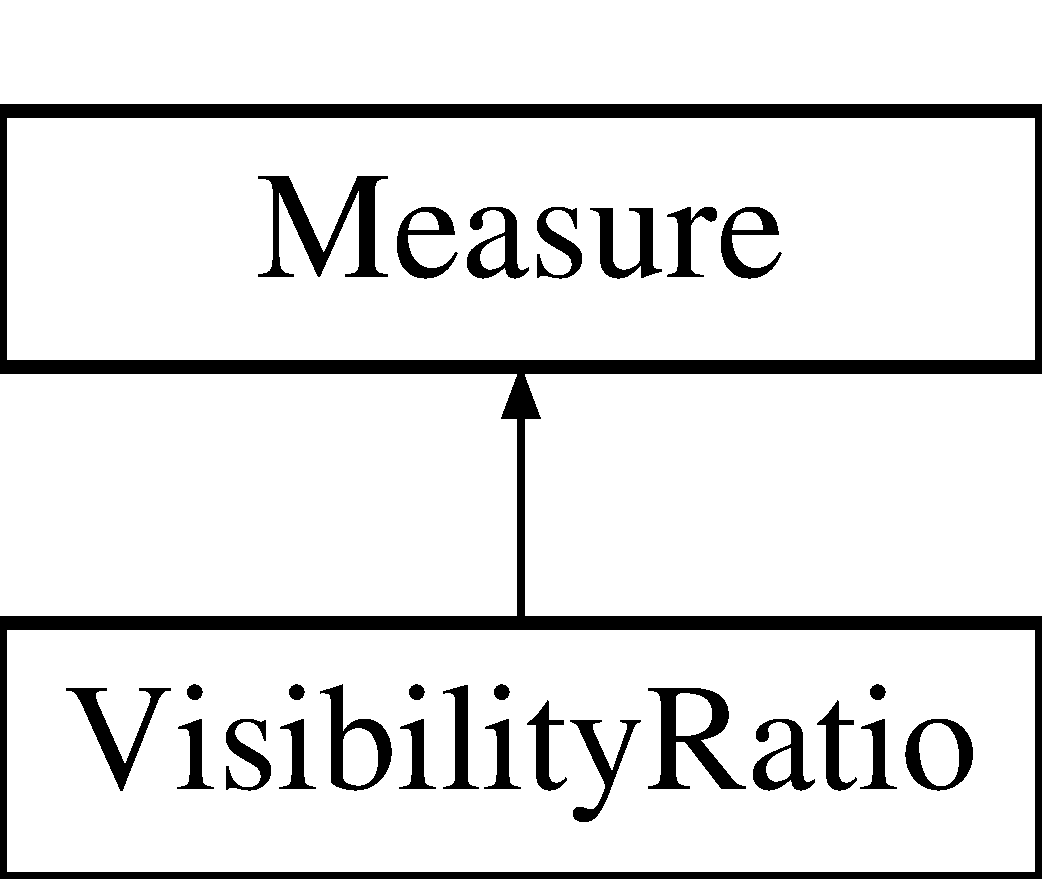
\includegraphics[height=2.000000cm]{class_visibility_ratio}
\end{center}
\end{figure}
\subsection*{Public Member Functions}
\begin{DoxyCompactItemize}
\item 
\hyperlink{class_visibility_ratio_a03d3d48318a5eec33804c1ddcca8e022}{Visibility\+Ratio} (const Q\+String \&p\+Name)
\begin{DoxyCompactList}\small\item\em Constructor. \end{DoxyCompactList}\item 
\hyperlink{class_visibility_ratio_ab77dfb1e013c6c0f8a2e4773040c3767}{$\sim$\+Visibility\+Ratio} ()
\begin{DoxyCompactList}\small\item\em Destructor. \end{DoxyCompactList}\item 
void \hyperlink{class_visibility_ratio_a4625fcd0353851a0f3fc65a5d8ec258e}{Compute} (const \hyperlink{class_scene_information_builder}{Scene\+Information\+Builder} $\ast$p\+Scene\+Information\+Builder)
\begin{DoxyCompactList}\small\item\em Method that computes the measure. \end{DoxyCompactList}\end{DoxyCompactItemize}
\subsection*{Additional Inherited Members}


\subsection{Detailed Description}
Class that implements the visibility ratio measures. 

\begin{DoxyAuthor}{Author}
Xavier Bonaventura 

Copyright\+: (c) Universitat de Girona 
\end{DoxyAuthor}


\subsection{Constructor \& Destructor Documentation}
\hypertarget{class_visibility_ratio_a03d3d48318a5eec33804c1ddcca8e022}{\index{Visibility\+Ratio@{Visibility\+Ratio}!Visibility\+Ratio@{Visibility\+Ratio}}
\index{Visibility\+Ratio@{Visibility\+Ratio}!Visibility\+Ratio@{Visibility\+Ratio}}
\subsubsection[{Visibility\+Ratio}]{\setlength{\rightskip}{0pt plus 5cm}Visibility\+Ratio\+::\+Visibility\+Ratio (
\begin{DoxyParamCaption}
\item[{const Q\+String \&}]{p\+Name}
\end{DoxyParamCaption}
)}}\label{class_visibility_ratio_a03d3d48318a5eec33804c1ddcca8e022}


Constructor. 

\hypertarget{class_visibility_ratio_ab77dfb1e013c6c0f8a2e4773040c3767}{\index{Visibility\+Ratio@{Visibility\+Ratio}!````~Visibility\+Ratio@{$\sim$\+Visibility\+Ratio}}
\index{````~Visibility\+Ratio@{$\sim$\+Visibility\+Ratio}!Visibility\+Ratio@{Visibility\+Ratio}}
\subsubsection[{$\sim$\+Visibility\+Ratio}]{\setlength{\rightskip}{0pt plus 5cm}Visibility\+Ratio\+::$\sim$\+Visibility\+Ratio (
\begin{DoxyParamCaption}
{}
\end{DoxyParamCaption}
)}}\label{class_visibility_ratio_ab77dfb1e013c6c0f8a2e4773040c3767}


Destructor. 



\subsection{Member Function Documentation}
\hypertarget{class_visibility_ratio_a4625fcd0353851a0f3fc65a5d8ec258e}{\index{Visibility\+Ratio@{Visibility\+Ratio}!Compute@{Compute}}
\index{Compute@{Compute}!Visibility\+Ratio@{Visibility\+Ratio}}
\subsubsection[{Compute}]{\setlength{\rightskip}{0pt plus 5cm}void Visibility\+Ratio\+::\+Compute (
\begin{DoxyParamCaption}
\item[{const {\bf Scene\+Information\+Builder} $\ast$}]{p\+Scene\+Information\+Builder}
\end{DoxyParamCaption}
)\hspace{0.3cm}{\ttfamily [virtual]}}}\label{class_visibility_ratio_a4625fcd0353851a0f3fc65a5d8ec258e}


Method that computes the measure. 



Implements \hyperlink{class_measure_aed88fe46b2a609ab5948e5f3c891321d}{Measure}.



The documentation for this class was generated from the following files\+:\begin{DoxyCompactItemize}
\item 
inc/viewpoint-\/measures/\hyperlink{_visibility_ratio_8h}{Visibility\+Ratio.\+h}\item 
src/viewpoint-\/measures/\hyperlink{_visibility_ratio_8cpp}{Visibility\+Ratio.\+cpp}\end{DoxyCompactItemize}

\hypertarget{class_v_m_i}{\section{V\+M\+I Class Reference}
\label{class_v_m_i}\index{V\+M\+I@{V\+M\+I}}
}


Class that implements the viewpoint mutual information \mbox{[}Feixas et al. 2009\mbox{]}.  




{\ttfamily \#include $<$V\+M\+I.\+h$>$}

Inheritance diagram for V\+M\+I\+:\begin{figure}[H]
\begin{center}
\leavevmode
\includegraphics[height=2.000000cm]{class_v_m_i}
\end{center}
\end{figure}
\subsection*{Public Member Functions}
\begin{DoxyCompactItemize}
\item 
\hyperlink{class_v_m_i_a3144eee2c59877b37ec2b8deb39b12dd}{V\+M\+I} (const Q\+String \&p\+Name)
\begin{DoxyCompactList}\small\item\em Constructor. \end{DoxyCompactList}\item 
\hyperlink{class_v_m_i_af3092d24c52726a06fff131a8271809d}{$\sim$\+V\+M\+I} ()
\begin{DoxyCompactList}\small\item\em Destructor. \end{DoxyCompactList}\item 
void \hyperlink{class_v_m_i_a8c3a1cc5b7cd97e4d53464354a275960}{Compute} (const \hyperlink{class_scene_information_builder}{Scene\+Information\+Builder} $\ast$p\+Scene\+Information\+Builder)
\begin{DoxyCompactList}\small\item\em Method that computes the measure. \end{DoxyCompactList}\end{DoxyCompactItemize}
\subsection*{Additional Inherited Members}


\subsection{Detailed Description}
Class that implements the viewpoint mutual information \mbox{[}Feixas et al. 2009\mbox{]}. 

\begin{DoxyAuthor}{Author}
Xavier Bonaventura 

Copyright\+: (c) Universitat de Girona 
\end{DoxyAuthor}


\subsection{Constructor \& Destructor Documentation}
\hypertarget{class_v_m_i_a3144eee2c59877b37ec2b8deb39b12dd}{\index{V\+M\+I@{V\+M\+I}!V\+M\+I@{V\+M\+I}}
\index{V\+M\+I@{V\+M\+I}!V\+M\+I@{V\+M\+I}}
\subsubsection[{V\+M\+I}]{\setlength{\rightskip}{0pt plus 5cm}V\+M\+I\+::\+V\+M\+I (
\begin{DoxyParamCaption}
\item[{const Q\+String \&}]{p\+Name}
\end{DoxyParamCaption}
)}}\label{class_v_m_i_a3144eee2c59877b37ec2b8deb39b12dd}


Constructor. 

\hypertarget{class_v_m_i_af3092d24c52726a06fff131a8271809d}{\index{V\+M\+I@{V\+M\+I}!````~V\+M\+I@{$\sim$\+V\+M\+I}}
\index{````~V\+M\+I@{$\sim$\+V\+M\+I}!V\+M\+I@{V\+M\+I}}
\subsubsection[{$\sim$\+V\+M\+I}]{\setlength{\rightskip}{0pt plus 5cm}V\+M\+I\+::$\sim$\+V\+M\+I (
\begin{DoxyParamCaption}
{}
\end{DoxyParamCaption}
)}}\label{class_v_m_i_af3092d24c52726a06fff131a8271809d}


Destructor. 



\subsection{Member Function Documentation}
\hypertarget{class_v_m_i_a8c3a1cc5b7cd97e4d53464354a275960}{\index{V\+M\+I@{V\+M\+I}!Compute@{Compute}}
\index{Compute@{Compute}!V\+M\+I@{V\+M\+I}}
\subsubsection[{Compute}]{\setlength{\rightskip}{0pt plus 5cm}void V\+M\+I\+::\+Compute (
\begin{DoxyParamCaption}
\item[{const {\bf Scene\+Information\+Builder} $\ast$}]{p\+Scene\+Information\+Builder}
\end{DoxyParamCaption}
)\hspace{0.3cm}{\ttfamily [virtual]}}}\label{class_v_m_i_a8c3a1cc5b7cd97e4d53464354a275960}


Method that computes the measure. 



Implements \hyperlink{class_measure_aed88fe46b2a609ab5948e5f3c891321d}{Measure}.



The documentation for this class was generated from the following files\+:\begin{DoxyCompactItemize}
\item 
inc/viewpoint-\/measures/\hyperlink{_v_m_i_8h}{V\+M\+I.\+h}\item 
src/viewpoint-\/measures/\hyperlink{_v_m_i_8cpp}{V\+M\+I.\+cpp}\end{DoxyCompactItemize}

\chapter{File Documentation}
\hypertarget{_axis_aligned_bounding_box_8h}{\section{inc/core/\+Axis\+Aligned\+Bounding\+Box.h File Reference}
\label{_axis_aligned_bounding_box_8h}\index{inc/core/\+Axis\+Aligned\+Bounding\+Box.\+h@{inc/core/\+Axis\+Aligned\+Bounding\+Box.\+h}}
}
{\ttfamily \#include \char`\"{}glm/vec3.\+hpp\char`\"{}}\\*
{\ttfamily \#include \char`\"{}Gizmo.\+h\char`\"{}}\\*
\subsection*{Classes}
\begin{DoxyCompactItemize}
\item 
class \hyperlink{class_axis_aligned_bounding_box}{Axis\+Aligned\+Bounding\+Box}
\begin{DoxyCompactList}\small\item\em Bounding\+Volume class with methods to use an axis-\/aligned bounding box. \end{DoxyCompactList}\end{DoxyCompactItemize}

\hypertarget{_bounding_sphere_8h}{\section{inc/core/\+Bounding\+Sphere.h File Reference}
\label{_bounding_sphere_8h}\index{inc/core/\+Bounding\+Sphere.\+h@{inc/core/\+Bounding\+Sphere.\+h}}
}
{\ttfamily \#include \char`\"{}glm/vec3.\+hpp\char`\"{}}\\*
{\ttfamily \#include \char`\"{}Gizmo.\+h\char`\"{}}\\*
\subsection*{Classes}
\begin{DoxyCompactItemize}
\item 
class \hyperlink{class_bounding_sphere}{Bounding\+Sphere}
\begin{DoxyCompactList}\small\item\em Bounding\+Volume class with methods to use a bounding sphere. \end{DoxyCompactList}\end{DoxyCompactItemize}

\hypertarget{_camera_8h}{\section{inc/core/\+Camera.h File Reference}
\label{_camera_8h}\index{inc/core/\+Camera.\+h@{inc/core/\+Camera.\+h}}
}
{\ttfamily \#include $<$Q\+String$>$}\\*
{\ttfamily \#include \char`\"{}glm/mat4x4.\+hpp\char`\"{}}\\*
{\ttfamily \#include \char`\"{}glm/vec3.\+hpp\char`\"{}}\\*
{\ttfamily \#include \char`\"{}Gizmo.\+h\char`\"{}}\\*
\subsection*{Classes}
\begin{DoxyCompactItemize}
\item 
class \hyperlink{class_camera}{Camera}
\begin{DoxyCompactList}\small\item\em Abstract camera class with methods to configure a generic camera. \end{DoxyCompactList}\end{DoxyCompactItemize}

\hypertarget{_camera_controller_8h}{\section{inc/core/\+Camera\+Controller.h File Reference}
\label{_camera_controller_8h}\index{inc/core/\+Camera\+Controller.\+h@{inc/core/\+Camera\+Controller.\+h}}
}
{\ttfamily \#include \char`\"{}Camera.\+h\char`\"{}}\\*
{\ttfamily \#include \char`\"{}G\+L\+Canvas.\+h\char`\"{}}\\*
\subsection*{Classes}
\begin{DoxyCompactItemize}
\item 
class \hyperlink{class_camera_controller}{Camera\+Controller}
\begin{DoxyCompactList}\small\item\em Generic class to control a camera. \end{DoxyCompactList}\end{DoxyCompactItemize}

\hypertarget{_debug_8h}{\section{inc/core/\+Debug.h File Reference}
\label{_debug_8h}\index{inc/core/\+Debug.\+h@{inc/core/\+Debug.\+h}}
}
{\ttfamily \#include $<$Q\+Plain\+Text\+Edit$>$}\\*
\subsection*{Classes}
\begin{DoxyCompactItemize}
\item 
class \hyperlink{class_debug}{Debug}
\begin{DoxyCompactList}\small\item\em Class to output log, warning and error messages through a console. \end{DoxyCompactList}\end{DoxyCompactItemize}
\subsection*{Macros}
\begin{DoxyCompactItemize}
\item 
\#define \hyperlink{_debug_8h_a2e19c69032dfd1589e65d2418308f61e}{C\+H\+E\+C\+K\+\_\+\+G\+L\+\_\+\+E\+R\+R\+O\+R}()
\end{DoxyCompactItemize}


\subsection{Macro Definition Documentation}
\hypertarget{_debug_8h_a2e19c69032dfd1589e65d2418308f61e}{\index{Debug.\+h@{Debug.\+h}!C\+H\+E\+C\+K\+\_\+\+G\+L\+\_\+\+E\+R\+R\+O\+R@{C\+H\+E\+C\+K\+\_\+\+G\+L\+\_\+\+E\+R\+R\+O\+R}}
\index{C\+H\+E\+C\+K\+\_\+\+G\+L\+\_\+\+E\+R\+R\+O\+R@{C\+H\+E\+C\+K\+\_\+\+G\+L\+\_\+\+E\+R\+R\+O\+R}!Debug.\+h@{Debug.\+h}}
\subsubsection[{C\+H\+E\+C\+K\+\_\+\+G\+L\+\_\+\+E\+R\+R\+O\+R}]{\setlength{\rightskip}{0pt plus 5cm}\#define C\+H\+E\+C\+K\+\_\+\+G\+L\+\_\+\+E\+R\+R\+O\+R(
\begin{DoxyParamCaption}
{}
\end{DoxyParamCaption}
)}}\label{_debug_8h_a2e19c69032dfd1589e65d2418308f61e}

\hypertarget{_geometry_8h}{\section{inc/core/\+Geometry.h File Reference}
\label{_geometry_8h}\index{inc/core/\+Geometry.\+h@{inc/core/\+Geometry.\+h}}
}
{\ttfamily \#include $<$Q\+Pair$>$}\\*
{\ttfamily \#include $<$Q\+String$>$}\\*
{\ttfamily \#include \char`\"{}glew.\+h\char`\"{}}\\*
{\ttfamily \#include \char`\"{}Axis\+Aligned\+Bounding\+Box.\+h\char`\"{}}\\*
{\ttfamily \#include \char`\"{}Bounding\+Sphere.\+h\char`\"{}}\\*
\subsection*{Classes}
\begin{DoxyCompactItemize}
\item 
class \hyperlink{class_geometry}{Geometry}
\begin{DoxyCompactList}\small\item\em Class to wrap the geometry of a 3d mesh that is not stored into the G\+P\+U until the Get\+G\+P\+U\+Geometry method is called. \end{DoxyCompactList}\end{DoxyCompactItemize}

\hypertarget{_gizmo_8h}{\section{inc/core/\+Gizmo.h File Reference}
\label{_gizmo_8h}\index{inc/core/\+Gizmo.\+h@{inc/core/\+Gizmo.\+h}}
}
{\ttfamily \#include $<$Q\+Vector$>$}\\*
{\ttfamily \#include \char`\"{}glm/vec4.\+hpp\char`\"{}}\\*
\subsection*{Classes}
\begin{DoxyCompactItemize}
\item 
class \hyperlink{class_gizmo}{Gizmo}
\begin{DoxyCompactList}\small\item\em A gizmo is a special element that can be rendered but without any kind of illumination. \end{DoxyCompactList}\end{DoxyCompactItemize}

\hypertarget{_g_l_canvas_8h}{\section{inc/core/\+G\+L\+Canvas.h File Reference}
\label{_g_l_canvas_8h}\index{inc/core/\+G\+L\+Canvas.\+h@{inc/core/\+G\+L\+Canvas.\+h}}
}
{\ttfamily \#include \char`\"{}glew.\+h\char`\"{}}\\*
{\ttfamily \#include $<$Q\+G\+L\+Widget$>$}\\*
{\ttfamily \#include $<$Q\+Vector$>$}\\*
{\ttfamily \#include \char`\"{}Camera.\+h\char`\"{}}\\*
{\ttfamily \#include \char`\"{}Geometry.\+h\char`\"{}}\\*
{\ttfamily \#include \char`\"{}G\+L\+S\+L\+Program.\+h\char`\"{}}\\*
{\ttfamily \#include \char`\"{}G\+P\+U\+Scene.\+h\char`\"{}}\\*
{\ttfamily \#include \char`\"{}Perspective\+Camera.\+h\char`\"{}}\\*
{\ttfamily \#include \char`\"{}Scene.\+h\char`\"{}}\\*
\subsection*{Classes}
\begin{DoxyCompactItemize}
\item 
class \hyperlink{class_g_l_canvas}{G\+L\+Canvas}
\begin{DoxyCompactList}\small\item\em Class to do the Open\+G\+L render. \end{DoxyCompactList}\end{DoxyCompactItemize}

\hypertarget{_g_l_s_l_program_8h}{\section{inc/core/\+G\+L\+S\+L\+Program.h File Reference}
\label{_g_l_s_l_program_8h}\index{inc/core/\+G\+L\+S\+L\+Program.\+h@{inc/core/\+G\+L\+S\+L\+Program.\+h}}
}
{\ttfamily \#include \char`\"{}glew.\+h\char`\"{}}\\*
{\ttfamily \#include $<$Q\+Hash$>$}\\*
{\ttfamily \#include $<$Q\+String$>$}\\*
{\ttfamily \#include $<$Q\+Vector$>$}\\*
{\ttfamily \#include \char`\"{}glm/mat4x4.\+hpp\char`\"{}}\\*
{\ttfamily \#include \char`\"{}G\+L\+S\+L\+Shader.\+h\char`\"{}}\\*
\subsection*{Classes}
\begin{DoxyCompactItemize}
\item 
class \hyperlink{class_g_l_s_l_program}{G\+L\+S\+L\+Program}
\begin{DoxyCompactList}\small\item\em Class to wrap the G\+L\+S\+L programs used by Open\+G\+L. \end{DoxyCompactList}\end{DoxyCompactItemize}

\hypertarget{_g_l_s_l_shader_8h}{\section{inc/core/\+G\+L\+S\+L\+Shader.h File Reference}
\label{_g_l_s_l_shader_8h}\index{inc/core/\+G\+L\+S\+L\+Shader.\+h@{inc/core/\+G\+L\+S\+L\+Shader.\+h}}
}
{\ttfamily \#include \char`\"{}glew.\+h\char`\"{}}\\*
{\ttfamily \#include $<$Q\+String$>$}\\*
\subsection*{Classes}
\begin{DoxyCompactItemize}
\item 
class \hyperlink{class_g_l_s_l_shader}{G\+L\+S\+L\+Shader}
\begin{DoxyCompactList}\small\item\em Class to wrap the G\+L\+S\+L shaders used by Open\+G\+L. \end{DoxyCompactList}\end{DoxyCompactItemize}

\hypertarget{_g_p_u_geometry_8h}{\section{inc/core/\+G\+P\+U\+Geometry.h File Reference}
\label{_g_p_u_geometry_8h}\index{inc/core/\+G\+P\+U\+Geometry.\+h@{inc/core/\+G\+P\+U\+Geometry.\+h}}
}
{\ttfamily \#include \char`\"{}glew.\+h\char`\"{}}\\*
{\ttfamily \#include \char`\"{}Geometry.\+h\char`\"{}}\\*
\subsection*{Classes}
\begin{DoxyCompactItemize}
\item 
class \hyperlink{class_g_p_u_geometry}{G\+P\+U\+Geometry}
\begin{DoxyCompactList}\small\item\em Class to wrap a \hyperlink{class_mesh}{Mesh} that is stored into the G\+P\+U. \end{DoxyCompactList}\end{DoxyCompactItemize}

\hypertarget{_g_p_u_scene_8h}{\section{inc/core/\+G\+P\+U\+Scene.h File Reference}
\label{_g_p_u_scene_8h}\index{inc/core/\+G\+P\+U\+Scene.\+h@{inc/core/\+G\+P\+U\+Scene.\+h}}
}
{\ttfamily \#include \char`\"{}G\+P\+U\+Scene\+Node.\+h\char`\"{}}\\*
{\ttfamily \#include \char`\"{}Scene.\+h\char`\"{}}\\*
\subsection*{Classes}
\begin{DoxyCompactItemize}
\item 
class \hyperlink{class_g_p_u_scene}{G\+P\+U\+Scene}
\end{DoxyCompactItemize}

\hypertarget{_g_p_u_scene_node_8h}{\section{inc/core/\+G\+P\+U\+Scene\+Node.h File Reference}
\label{_g_p_u_scene_node_8h}\index{inc/core/\+G\+P\+U\+Scene\+Node.\+h@{inc/core/\+G\+P\+U\+Scene\+Node.\+h}}
}
{\ttfamily \#include \char`\"{}glew.\+h\char`\"{}}\\*
{\ttfamily \#include \char`\"{}glm/mat4x4.\+hpp\char`\"{}}\\*
{\ttfamily \#include \char`\"{}G\+P\+U\+Geometry.\+h\char`\"{}}\\*
{\ttfamily \#include \char`\"{}Material.\+h\char`\"{}}\\*
\subsection*{Classes}
\begin{DoxyCompactItemize}
\item 
class \hyperlink{class_g_p_u_scene_node}{G\+P\+U\+Scene\+Node}
\end{DoxyCompactItemize}

\hypertarget{_material_8h}{\section{inc/core/\+Material.h File Reference}
\label{_material_8h}\index{inc/core/\+Material.\+h@{inc/core/\+Material.\+h}}
}
{\ttfamily \#include $<$Q\+String$>$}\\*
{\ttfamily \#include $<$Q\+Image$>$}\\*
{\ttfamily \#include \char`\"{}glm/vec3.\+hpp\char`\"{}}\\*
{\ttfamily \#include \char`\"{}Texture.\+h\char`\"{}}\\*
\subsection*{Classes}
\begin{DoxyCompactItemize}
\item 
class \hyperlink{class_material}{Material}
\begin{DoxyCompactList}\small\item\em Class to wrap the material of a mesh. \end{DoxyCompactList}\end{DoxyCompactItemize}

\hypertarget{_mesh_8h}{\section{inc/core/\+Mesh.h File Reference}
\label{_mesh_8h}\index{inc/core/\+Mesh.\+h@{inc/core/\+Mesh.\+h}}
}
{\ttfamily \#include $<$Q\+String$>$}\\*
{\ttfamily \#include \char`\"{}Geometry.\+h\char`\"{}}\\*
{\ttfamily \#include \char`\"{}Material.\+h\char`\"{}}\\*
\subsection*{Classes}
\begin{DoxyCompactItemize}
\item 
class \hyperlink{class_mesh}{Mesh}
\begin{DoxyCompactList}\small\item\em Class to wrap a 3d mesh. \end{DoxyCompactList}\end{DoxyCompactItemize}

\hypertarget{_orthographic_camera_8h}{\section{inc/core/\+Orthographic\+Camera.h File Reference}
\label{_orthographic_camera_8h}\index{inc/core/\+Orthographic\+Camera.\+h@{inc/core/\+Orthographic\+Camera.\+h}}
}
{\ttfamily \#include \char`\"{}Camera.\+h\char`\"{}}\\*
\subsection*{Classes}
\begin{DoxyCompactItemize}
\item 
class \hyperlink{class_orthographic_camera}{Orthographic\+Camera}
\begin{DoxyCompactList}\small\item\em \hyperlink{class_camera}{Camera} class with methods to configure an orthographic camera. \end{DoxyCompactList}\end{DoxyCompactItemize}

\hypertarget{_perspective_camera_8h}{\section{inc/core/\+Perspective\+Camera.h File Reference}
\label{_perspective_camera_8h}\index{inc/core/\+Perspective\+Camera.\+h@{inc/core/\+Perspective\+Camera.\+h}}
}
{\ttfamily \#include \char`\"{}Camera.\+h\char`\"{}}\\*
\subsection*{Classes}
\begin{DoxyCompactItemize}
\item 
class \hyperlink{class_perspective_camera}{Perspective\+Camera}
\begin{DoxyCompactList}\small\item\em \hyperlink{class_camera}{Camera} class with methods to configure a perspective camera. \end{DoxyCompactList}\end{DoxyCompactItemize}

\hypertarget{_scene_8h}{\section{inc/core/\+Scene.h File Reference}
\label{_scene_8h}\index{inc/core/\+Scene.\+h@{inc/core/\+Scene.\+h}}
}
{\ttfamily \#include $<$Q\+String$>$}\\*
{\ttfamily \#include \char`\"{}Bounding\+Sphere.\+h\char`\"{}}\\*
{\ttfamily \#include \char`\"{}Scene\+Node.\+h\char`\"{}}\\*
\subsection*{Classes}
\begin{DoxyCompactItemize}
\item 
class \hyperlink{class_scene}{Scene}
\begin{DoxyCompactList}\small\item\em Class representing a scene. \end{DoxyCompactList}\end{DoxyCompactItemize}

\hypertarget{_scene_loader_8h}{\section{inc/core/\+Scene\+Loader.h File Reference}
\label{_scene_loader_8h}\index{inc/core/\+Scene\+Loader.\+h@{inc/core/\+Scene\+Loader.\+h}}
}
{\ttfamily \#include $<$Q\+String$>$}\\*
{\ttfamily \#include $<$Q\+Vector$>$}\\*
{\ttfamily \#include \char`\"{}assimp/material.\+h\char`\"{}}\\*
{\ttfamily \#include \char`\"{}assimp/scene.\+h\char`\"{}}\\*
{\ttfamily \#include \char`\"{}Geometry.\+h\char`\"{}}\\*
{\ttfamily \#include \char`\"{}Material.\+h\char`\"{}}\\*
{\ttfamily \#include \char`\"{}Mesh.\+h\char`\"{}}\\*
{\ttfamily \#include \char`\"{}Scene.\+h\char`\"{}}\\*
\subsection*{Classes}
\begin{DoxyCompactItemize}
\item 
class \hyperlink{class_scene_loader}{Scene\+Loader}
\begin{DoxyCompactList}\small\item\em Class to load scenes from files. \end{DoxyCompactList}\end{DoxyCompactItemize}

\hypertarget{_scene_node_8h}{\section{inc/core/\+Scene\+Node.h File Reference}
\label{_scene_node_8h}\index{inc/core/\+Scene\+Node.\+h@{inc/core/\+Scene\+Node.\+h}}
}
{\ttfamily \#include $<$Q\+String$>$}\\*
{\ttfamily \#include $<$Q\+Vector$>$}\\*
{\ttfamily \#include \char`\"{}Camera.\+h\char`\"{}}\\*
{\ttfamily \#include \char`\"{}Mesh.\+h\char`\"{}}\\*
\subsection*{Classes}
\begin{DoxyCompactItemize}
\item 
class \hyperlink{class_scene_node}{Scene\+Node}
\begin{DoxyCompactList}\small\item\em Class for a node of a scene. \end{DoxyCompactList}\end{DoxyCompactItemize}

\hypertarget{_serialized_scene_geometry_8h}{\section{inc/core/\+Serialized\+Scene\+Geometry.h File Reference}
\label{_serialized_scene_geometry_8h}\index{inc/core/\+Serialized\+Scene\+Geometry.\+h@{inc/core/\+Serialized\+Scene\+Geometry.\+h}}
}
{\ttfamily \#include \char`\"{}Scene.\+h\char`\"{}}\\*
\subsection*{Classes}
\begin{DoxyCompactItemize}
\item 
class \hyperlink{class_serialized_scene_geometry}{Serialized\+Scene\+Geometry}
\end{DoxyCompactItemize}

\hypertarget{_texture_8h}{\section{inc/core/\+Texture.h File Reference}
\label{_texture_8h}\index{inc/core/\+Texture.\+h@{inc/core/\+Texture.\+h}}
}
{\ttfamily \#include \char`\"{}glew.\+h\char`\"{}}\\*
{\ttfamily \#include $<$Q\+Image$>$}\\*
\subsection*{Classes}
\begin{DoxyCompactItemize}
\item 
class \hyperlink{class_texture}{Texture}
\begin{DoxyCompactList}\small\item\em Class to wrap an Open\+G\+L texture. \end{DoxyCompactList}\end{DoxyCompactItemize}

\hypertarget{_trackball_camera_8h}{\section{inc/core/\+Trackball\+Camera.h File Reference}
\label{_trackball_camera_8h}\index{inc/core/\+Trackball\+Camera.\+h@{inc/core/\+Trackball\+Camera.\+h}}
}
{\ttfamily \#include \char`\"{}Camera\+Controller.\+h\char`\"{}}\\*
\subsection*{Classes}
\begin{DoxyCompactItemize}
\item 
class \hyperlink{class_trackball_camera}{Trackball\+Camera}
\end{DoxyCompactItemize}

\hypertarget{_dutagaci_dialog_8h}{\section{inc/\+Dutagaci\+Dialog.h File Reference}
\label{_dutagaci_dialog_8h}\index{inc/\+Dutagaci\+Dialog.\+h@{inc/\+Dutagaci\+Dialog.\+h}}
}
{\ttfamily \#include \char`\"{}ui\+\_\+\+Dutagaci\+View.\+h\char`\"{}}\\*
{\ttfamily \#include $<$Q\+Dialog$>$}\\*
{\ttfamily \#include $<$Q\+File\+Dialog$>$}\\*
\subsection*{Classes}
\begin{DoxyCompactItemize}
\item 
class \hyperlink{class_dutagaci_dialog}{Dutagaci\+Dialog}
\begin{DoxyCompactList}\small\item\em Dialog to run the Dutagaci benchmark. \end{DoxyCompactList}\end{DoxyCompactItemize}
\subsection*{Namespaces}
\begin{DoxyCompactItemize}
\item 
 \hyperlink{namespace_ui}{Ui}
\end{DoxyCompactItemize}

\hypertarget{_main_module_controller_8h}{\section{inc/\+Main\+Module\+Controller.h File Reference}
\label{_main_module_controller_8h}\index{inc/\+Main\+Module\+Controller.\+h@{inc/\+Main\+Module\+Controller.\+h}}
}
{\ttfamily \#include \char`\"{}ui\+\_\+\+Main\+Module.\+h\char`\"{}}\\*
{\ttfamily \#include $<$Q\+Signal\+Mapper$>$}\\*
{\ttfamily \#include \char`\"{}Dutagaci\+Dialog.\+h\char`\"{}}\\*
{\ttfamily \#include \char`\"{}G\+L\+Canvas.\+h\char`\"{}}\\*
{\ttfamily \#include \char`\"{}Measure.\+h\char`\"{}}\\*
{\ttfamily \#include \char`\"{}Module\+Controller.\+h\char`\"{}}\\*
{\ttfamily \#include \char`\"{}Scene\+Information\+Builder.\+h\char`\"{}}\\*
{\ttfamily \#include \char`\"{}Sphere\+Of\+Viewpoints.\+h\char`\"{}}\\*
\subsection*{Classes}
\begin{DoxyCompactItemize}
\item 
class \hyperlink{class_main_module_controller}{Main\+Module\+Controller}
\begin{DoxyCompactList}\small\item\em Controller for the view of the main module. \end{DoxyCompactList}\end{DoxyCompactItemize}
\subsection*{Namespaces}
\begin{DoxyCompactItemize}
\item 
 \hyperlink{namespace_ui}{Ui}
\end{DoxyCompactItemize}

\hypertarget{_main_window_8h}{\section{inc/\+Main\+Window.h File Reference}
\label{_main_window_8h}\index{inc/\+Main\+Window.\+h@{inc/\+Main\+Window.\+h}}
}
{\ttfamily \#include \char`\"{}ui\+\_\+\+Main\+Window.\+h\char`\"{}}\\*
{\ttfamily \#include $<$Q\+Main\+Window$>$}\\*
{\ttfamily \#include \char`\"{}Module\+Tab\+Widget.\+h\char`\"{}}\\*
\subsection*{Classes}
\begin{DoxyCompactItemize}
\item 
class \hyperlink{class_main_window}{Main\+Window}
\begin{DoxyCompactList}\small\item\em Main class of the project. \end{DoxyCompactList}\end{DoxyCompactItemize}
\subsection*{Namespaces}
\begin{DoxyCompactItemize}
\item 
 \hyperlink{namespace_ui}{Ui}
\end{DoxyCompactItemize}

\hypertarget{_measure_8h}{\section{inc/\+Measure.h File Reference}
\label{_measure_8h}\index{inc/\+Measure.\+h@{inc/\+Measure.\+h}}
}
{\ttfamily \#include $<$Q\+String$>$}\\*
{\ttfamily \#include \char`\"{}Scene\+Information\+Builder.\+h\char`\"{}}\\*
\subsection*{Classes}
\begin{DoxyCompactItemize}
\item 
class \hyperlink{class_measure}{Measure}
\begin{DoxyCompactList}\small\item\em Parent class for all the measures. \end{DoxyCompactList}\end{DoxyCompactItemize}

\hypertarget{_module_controller_8h}{\section{inc/\+Module\+Controller.h File Reference}
\label{_module_controller_8h}\index{inc/\+Module\+Controller.\+h@{inc/\+Module\+Controller.\+h}}
}
{\ttfamily \#include $<$Q\+Menu$>$}\\*
{\ttfamily \#include $<$Q\+Widget$>$}\\*
\subsection*{Classes}
\begin{DoxyCompactItemize}
\item 
class \hyperlink{class_module_controller}{Module\+Controller}
\end{DoxyCompactItemize}

\hypertarget{_module_tab_widget_8h}{\section{inc/\+Module\+Tab\+Widget.h File Reference}
\label{_module_tab_widget_8h}\index{inc/\+Module\+Tab\+Widget.\+h@{inc/\+Module\+Tab\+Widget.\+h}}
}
{\ttfamily \#include $<$Q\+Map$>$}\\*
{\ttfamily \#include $<$Q\+Tab\+Widget$>$}\\*
\subsection*{Classes}
\begin{DoxyCompactItemize}
\item 
class \hyperlink{class_module_tab_widget}{Module\+Tab\+Widget}
\begin{DoxyCompactList}\small\item\em Class to handle the different moudles that you can load in the program using different tabs. \end{DoxyCompactList}\end{DoxyCompactItemize}

\hypertarget{_projected_areas_matrix_8h}{\section{inc/\+Projected\+Areas\+Matrix.h File Reference}
\label{_projected_areas_matrix_8h}\index{inc/\+Projected\+Areas\+Matrix.\+h@{inc/\+Projected\+Areas\+Matrix.\+h}}
}
{\ttfamily \#include $<$Q\+Vector$>$}\\*
\subsection*{Classes}
\begin{DoxyCompactItemize}
\item 
class \hyperlink{class_projected_areas_matrix}{Projected\+Areas\+Matrix}
\end{DoxyCompactItemize}

\hypertarget{_scene_information_builder_8h}{\section{inc/\+Scene\+Information\+Builder.h File Reference}
\label{_scene_information_builder_8h}\index{inc/\+Scene\+Information\+Builder.\+h@{inc/\+Scene\+Information\+Builder.\+h}}
}
{\ttfamily \#include \char`\"{}opencv2/core/core.\+hpp\char`\"{}}\\*
{\ttfamily \#include \char`\"{}G\+L\+S\+L\+Program.\+h\char`\"{}}\\*
{\ttfamily \#include \char`\"{}Projected\+Areas\+Matrix.\+h\char`\"{}}\\*
{\ttfamily \#include \char`\"{}Scene.\+h\char`\"{}}\\*
{\ttfamily \#include \char`\"{}Serialized\+Scene\+Geometry.\+h\char`\"{}}\\*
{\ttfamily \#include \char`\"{}Sphere\+Of\+Viewpoints.\+h\char`\"{}}\\*
\subsection*{Classes}
\begin{DoxyCompactItemize}
\item 
class \hyperlink{class_scene_information_builder}{Scene\+Information\+Builder}
\begin{DoxyCompactList}\small\item\em Static class to create an Information\+Channel\+Histogram. \end{DoxyCompactList}\end{DoxyCompactItemize}

\hypertarget{_sphere_of_viewpoints_8h}{\section{inc/\+Sphere\+Of\+Viewpoints.h File Reference}
\label{_sphere_of_viewpoints_8h}\index{inc/\+Sphere\+Of\+Viewpoints.\+h@{inc/\+Sphere\+Of\+Viewpoints.\+h}}
}
{\ttfamily \#include \char`\"{}Camera.\+h\char`\"{}}\\*
{\ttfamily \#include \char`\"{}Sphere\+Point\+Cloud.\+h\char`\"{}}\\*
\subsection*{Classes}
\begin{DoxyCompactItemize}
\item 
class \hyperlink{class_sphere_of_viewpoints}{Sphere\+Of\+Viewpoints}
\end{DoxyCompactItemize}

\hypertarget{_sphere_point_cloud_8h}{\section{inc/\+Sphere\+Point\+Cloud.h File Reference}
\label{_sphere_point_cloud_8h}\index{inc/\+Sphere\+Point\+Cloud.\+h@{inc/\+Sphere\+Point\+Cloud.\+h}}
}
{\ttfamily \#include $<$Q\+Vector$>$}\\*
{\ttfamily \#include \char`\"{}Geometry.\+h\char`\"{}}\\*
\subsection*{Classes}
\begin{DoxyCompactItemize}
\item 
class \hyperlink{class_sphere_point_cloud}{Sphere\+Point\+Cloud}
\end{DoxyCompactItemize}

\hypertarget{_tools_8h}{\section{inc/\+Tools.h File Reference}
\label{_tools_8h}\index{inc/\+Tools.\+h@{inc/\+Tools.\+h}}
}
{\ttfamily \#include $<$Q\+Pair$>$}\\*
{\ttfamily \#include $<$Q\+Vector$>$}\\*
{\ttfamily \#include \char`\"{}glm/vec3.\+hpp\char`\"{}}\\*
\subsection*{Classes}
\begin{DoxyCompactItemize}
\item 
class \hyperlink{class_tools}{Tools}
\end{DoxyCompactItemize}

\hypertarget{_curvature_entropy_8h}{\section{inc/viewpoint-\/measures/\+Curvature\+Entropy.h File Reference}
\label{_curvature_entropy_8h}\index{inc/viewpoint-\/measures/\+Curvature\+Entropy.\+h@{inc/viewpoint-\/measures/\+Curvature\+Entropy.\+h}}
}
{\ttfamily \#include \char`\"{}Measure.\+h\char`\"{}}\\*
\subsection*{Classes}
\begin{DoxyCompactItemize}
\item 
class \hyperlink{class_curvature_entropy}{Curvature\+Entropy}
\begin{DoxyCompactList}\small\item\em Class that implements the curvature entropy measure. \end{DoxyCompactList}\end{DoxyCompactItemize}

\hypertarget{_depth_based_visual_stability_8h}{\section{inc/viewpoint-\/measures/\+Depth\+Based\+Visual\+Stability.h File Reference}
\label{_depth_based_visual_stability_8h}\index{inc/viewpoint-\/measures/\+Depth\+Based\+Visual\+Stability.\+h@{inc/viewpoint-\/measures/\+Depth\+Based\+Visual\+Stability.\+h}}
}
{\ttfamily \#include \char`\"{}Measure.\+h\char`\"{}}\\*
\subsection*{Classes}
\begin{DoxyCompactItemize}
\item 
class \hyperlink{class_depth_based_visual_stability}{Depth\+Based\+Visual\+Stability}
\end{DoxyCompactItemize}

\hypertarget{_depth_distribution_8h}{\section{inc/viewpoint-\/measures/\+Depth\+Distribution.h File Reference}
\label{_depth_distribution_8h}\index{inc/viewpoint-\/measures/\+Depth\+Distribution.\+h@{inc/viewpoint-\/measures/\+Depth\+Distribution.\+h}}
}
{\ttfamily \#include \char`\"{}Measure.\+h\char`\"{}}\\*
\subsection*{Classes}
\begin{DoxyCompactItemize}
\item 
class \hyperlink{class_depth_distribution}{Depth\+Distribution}
\begin{DoxyCompactList}\small\item\em Class that implements the depth distribution \mbox{[}Secord et al. 2011\mbox{]}. \end{DoxyCompactList}\end{DoxyCompactItemize}

\hypertarget{_feixas_saliency_8h}{\section{inc/viewpoint-\/measures/\+Feixas\+Saliency.h File Reference}
\label{_feixas_saliency_8h}\index{inc/viewpoint-\/measures/\+Feixas\+Saliency.\+h@{inc/viewpoint-\/measures/\+Feixas\+Saliency.\+h}}
}
{\ttfamily \#include \char`\"{}Measure.\+h\char`\"{}}\\*
\subsection*{Classes}
\begin{DoxyCompactItemize}
\item 
class \hyperlink{class_feixas_saliency}{Feixas\+Saliency}
\begin{DoxyCompactList}\small\item\em Class that implements the saliency of a viewpoint \mbox{[}Feixas et al. 2009\mbox{]}. \end{DoxyCompactList}\end{DoxyCompactItemize}

\hypertarget{_heuristic_measure_8h}{\section{inc/viewpoint-\/measures/\+Heuristic\+Measure.h File Reference}
\label{_heuristic_measure_8h}\index{inc/viewpoint-\/measures/\+Heuristic\+Measure.\+h@{inc/viewpoint-\/measures/\+Heuristic\+Measure.\+h}}
}
{\ttfamily \#include \char`\"{}Measure.\+h\char`\"{}}\\*
\subsection*{Classes}
\begin{DoxyCompactItemize}
\item 
class \hyperlink{class_heuristic_measure}{Heuristic\+Measure}
\begin{DoxyCompactList}\small\item\em Class that implements the heuristic measure \mbox{[}Plemenos and Benayada 1996\mbox{]}. \end{DoxyCompactList}\end{DoxyCompactItemize}

\hypertarget{_i2_8h}{\section{inc/viewpoint-\/measures/\+I2.h File Reference}
\label{_i2_8h}\index{inc/viewpoint-\/measures/\+I2.\+h@{inc/viewpoint-\/measures/\+I2.\+h}}
}
{\ttfamily \#include \char`\"{}Measure.\+h\char`\"{}}\\*
\subsection*{Classes}
\begin{DoxyCompactItemize}
\item 
class \hyperlink{class_i2}{I2}
\begin{DoxyCompactList}\small\item\em Class that implements the \hyperlink{class_i2}{I2} measure \mbox{[}Bonaventura et al. 2011\mbox{]}. \end{DoxyCompactList}\end{DoxyCompactItemize}

\hypertarget{_i3_8h}{\section{inc/viewpoint-\/measures/\+I3.h File Reference}
\label{_i3_8h}\index{inc/viewpoint-\/measures/\+I3.\+h@{inc/viewpoint-\/measures/\+I3.\+h}}
}
{\ttfamily \#include \char`\"{}Measure.\+h\char`\"{}}\\*
\subsection*{Classes}
\begin{DoxyCompactItemize}
\item 
class \hyperlink{class_i3}{I3}
\begin{DoxyCompactList}\small\item\em Class that implements the \hyperlink{class_i3}{I3} measure \mbox{[}Bonaventura et al. 2011\mbox{]}. \end{DoxyCompactList}\end{DoxyCompactItemize}

\hypertarget{_kullback_leibler_8h}{\section{inc/viewpoint-\/measures/\+Kullback\+Leibler.h File Reference}
\label{_kullback_leibler_8h}\index{inc/viewpoint-\/measures/\+Kullback\+Leibler.\+h@{inc/viewpoint-\/measures/\+Kullback\+Leibler.\+h}}
}
{\ttfamily \#include \char`\"{}Measure.\+h\char`\"{}}\\*
\subsection*{Classes}
\begin{DoxyCompactItemize}
\item 
class \hyperlink{class_kullback_leibler}{Kullback\+Leibler}
\begin{DoxyCompactList}\small\item\em Class that implements the kullback leibler distance \mbox{[}Sbert et al. 2005\mbox{]}. \end{DoxyCompactList}\end{DoxyCompactItemize}

\hypertarget{_maximum_depth_8h}{\section{inc/viewpoint-\/measures/\+Maximum\+Depth.h File Reference}
\label{_maximum_depth_8h}\index{inc/viewpoint-\/measures/\+Maximum\+Depth.\+h@{inc/viewpoint-\/measures/\+Maximum\+Depth.\+h}}
}
{\ttfamily \#include \char`\"{}Measure.\+h\char`\"{}}\\*
\subsection*{Classes}
\begin{DoxyCompactItemize}
\item 
class \hyperlink{class_maximum_depth}{Maximum\+Depth}
\begin{DoxyCompactList}\small\item\em Class that implements the maximum depth measure. \end{DoxyCompactList}\end{DoxyCompactItemize}

\hypertarget{_number_of_visible_triangles_8h}{\section{inc/viewpoint-\/measures/\+Number\+Of\+Visible\+Triangles.h File Reference}
\label{_number_of_visible_triangles_8h}\index{inc/viewpoint-\/measures/\+Number\+Of\+Visible\+Triangles.\+h@{inc/viewpoint-\/measures/\+Number\+Of\+Visible\+Triangles.\+h}}
}
{\ttfamily \#include \char`\"{}Measure.\+h\char`\"{}}\\*
\subsection*{Classes}
\begin{DoxyCompactItemize}
\item 
class \hyperlink{class_number_of_visible_triangles}{Number\+Of\+Visible\+Triangles}
\begin{DoxyCompactList}\small\item\em Class that implements the number of visible triangles measures. \end{DoxyCompactList}\end{DoxyCompactItemize}

\hypertarget{_projected_area_8h}{\section{inc/viewpoint-\/measures/\+Projected\+Area.h File Reference}
\label{_projected_area_8h}\index{inc/viewpoint-\/measures/\+Projected\+Area.\+h@{inc/viewpoint-\/measures/\+Projected\+Area.\+h}}
}
{\ttfamily \#include \char`\"{}Measure.\+h\char`\"{}}\\*
\subsection*{Classes}
\begin{DoxyCompactItemize}
\item 
class \hyperlink{class_projected_area}{Projected\+Area}
\begin{DoxyCompactList}\small\item\em Class that implements the projected area measure. \end{DoxyCompactList}\end{DoxyCompactItemize}

\input{_saliency_e_v_m_i_8h}
\hypertarget{_silhouette_curvature_8h}{\section{inc/viewpoint-\/measures/\+Silhouette\+Curvature.h File Reference}
\label{_silhouette_curvature_8h}\index{inc/viewpoint-\/measures/\+Silhouette\+Curvature.\+h@{inc/viewpoint-\/measures/\+Silhouette\+Curvature.\+h}}
}
{\ttfamily \#include \char`\"{}Measure.\+h\char`\"{}}\\*
\subsection*{Classes}
\begin{DoxyCompactItemize}
\item 
class \hyperlink{class_silhouette_curvature}{Silhouette\+Curvature}
\begin{DoxyCompactList}\small\item\em Class that implements the silhouette curvature measure. \end{DoxyCompactList}\end{DoxyCompactItemize}

\hypertarget{_silhouette_curvature_extrema_8h}{\section{inc/viewpoint-\/measures/\+Silhouette\+Curvature\+Extrema.h File Reference}
\label{_silhouette_curvature_extrema_8h}\index{inc/viewpoint-\/measures/\+Silhouette\+Curvature\+Extrema.\+h@{inc/viewpoint-\/measures/\+Silhouette\+Curvature\+Extrema.\+h}}
}
{\ttfamily \#include \char`\"{}Measure.\+h\char`\"{}}\\*
\subsection*{Classes}
\begin{DoxyCompactItemize}
\item 
class \hyperlink{class_silhouette_curvature_extrema}{Silhouette\+Curvature\+Extrema}
\begin{DoxyCompactList}\small\item\em Class that implements the silhouette curvature extrema. \end{DoxyCompactList}\end{DoxyCompactItemize}

\hypertarget{_silhouette_entropy_8h}{\section{inc/viewpoint-\/measures/\+Silhouette\+Entropy.h File Reference}
\label{_silhouette_entropy_8h}\index{inc/viewpoint-\/measures/\+Silhouette\+Entropy.\+h@{inc/viewpoint-\/measures/\+Silhouette\+Entropy.\+h}}
}
{\ttfamily \#include \char`\"{}Measure.\+h\char`\"{}}\\*
\subsection*{Classes}
\begin{DoxyCompactItemize}
\item 
class \hyperlink{class_silhouette_entropy}{Silhouette\+Entropy}
\begin{DoxyCompactList}\small\item\em Class that implements the silhouette entropy measure. \end{DoxyCompactList}\end{DoxyCompactItemize}

\hypertarget{_silhouette_length_8h}{\section{inc/viewpoint-\/measures/\+Silhouette\+Length.h File Reference}
\label{_silhouette_length_8h}\index{inc/viewpoint-\/measures/\+Silhouette\+Length.\+h@{inc/viewpoint-\/measures/\+Silhouette\+Length.\+h}}
}
{\ttfamily \#include \char`\"{}Measure.\+h\char`\"{}}\\*
\subsection*{Classes}
\begin{DoxyCompactItemize}
\item 
class \hyperlink{class_silhouette_length}{Silhouette\+Length}
\begin{DoxyCompactList}\small\item\em Class that implements the silhouette length measure. \end{DoxyCompactList}\end{DoxyCompactItemize}

\hypertarget{_stoev_strasser_8h}{\section{inc/viewpoint-\/measures/\+Stoev\+Strasser.h File Reference}
\label{_stoev_strasser_8h}\index{inc/viewpoint-\/measures/\+Stoev\+Strasser.\+h@{inc/viewpoint-\/measures/\+Stoev\+Strasser.\+h}}
}
{\ttfamily \#include \char`\"{}Measure.\+h\char`\"{}}\\*
\subsection*{Classes}
\begin{DoxyCompactItemize}
\item 
class \hyperlink{class_stoev_strasser}{Stoev\+Strasser}
\begin{DoxyCompactList}\small\item\em Class that implements the Stoev and Strasser measure \mbox{[}Stoev and Strasser 2002\mbox{]}. \end{DoxyCompactList}\end{DoxyCompactItemize}

\hypertarget{_unstability_8h}{\section{inc/viewpoint-\/measures/\+Unstability.h File Reference}
\label{_unstability_8h}\index{inc/viewpoint-\/measures/\+Unstability.\+h@{inc/viewpoint-\/measures/\+Unstability.\+h}}
}
{\ttfamily \#include \char`\"{}Measure.\+h\char`\"{}}\\*
\subsection*{Classes}
\begin{DoxyCompactItemize}
\item 
class \hyperlink{class_unstability}{Unstability}
\begin{DoxyCompactList}\small\item\em Class that implements the unstability measure \mbox{[}Feixas et al. 2009\mbox{]}. \end{DoxyCompactList}\end{DoxyCompactItemize}

\hypertarget{_viewpoint_entropy_8h}{\section{inc/viewpoint-\/measures/\+Viewpoint\+Entropy.h File Reference}
\label{_viewpoint_entropy_8h}\index{inc/viewpoint-\/measures/\+Viewpoint\+Entropy.\+h@{inc/viewpoint-\/measures/\+Viewpoint\+Entropy.\+h}}
}
{\ttfamily \#include \char`\"{}Measure.\+h\char`\"{}}\\*
\subsection*{Classes}
\begin{DoxyCompactItemize}
\item 
class \hyperlink{class_viewpoint_entropy}{Viewpoint\+Entropy}
\begin{DoxyCompactList}\small\item\em Class that implements the viewpoint entropy \mbox{[}Vázquez et al. 2002\mbox{]}. \end{DoxyCompactList}\end{DoxyCompactItemize}

\hypertarget{_visibility_ratio_8h}{\section{inc/viewpoint-\/measures/\+Visibility\+Ratio.h File Reference}
\label{_visibility_ratio_8h}\index{inc/viewpoint-\/measures/\+Visibility\+Ratio.\+h@{inc/viewpoint-\/measures/\+Visibility\+Ratio.\+h}}
}
{\ttfamily \#include \char`\"{}Measure.\+h\char`\"{}}\\*
\subsection*{Classes}
\begin{DoxyCompactItemize}
\item 
class \hyperlink{class_visibility_ratio}{Visibility\+Ratio}
\begin{DoxyCompactList}\small\item\em Class that implements the visibility ratio measures. \end{DoxyCompactList}\end{DoxyCompactItemize}

\hypertarget{_v_m_i_8h}{\section{inc/viewpoint-\/measures/\+V\+M\+I.h File Reference}
\label{_v_m_i_8h}\index{inc/viewpoint-\/measures/\+V\+M\+I.\+h@{inc/viewpoint-\/measures/\+V\+M\+I.\+h}}
}
{\ttfamily \#include \char`\"{}Measure.\+h\char`\"{}}\\*
\subsection*{Classes}
\begin{DoxyCompactItemize}
\item 
class \hyperlink{class_v_m_i}{V\+M\+I}
\begin{DoxyCompactList}\small\item\em Class that implements the viewpoint mutual information \mbox{[}Feixas et al. 2009\mbox{]}. \end{DoxyCompactList}\end{DoxyCompactItemize}

\hypertarget{_viewpoint_measure_slider_8h}{\section{inc/\+Viewpoint\+Measure\+Slider.h File Reference}
\label{_viewpoint_measure_slider_8h}\index{inc/\+Viewpoint\+Measure\+Slider.\+h@{inc/\+Viewpoint\+Measure\+Slider.\+h}}
}
{\ttfamily \#include $<$Q\+Slider$>$}\\*
\subsection*{Classes}
\begin{DoxyCompactItemize}
\item 
class \hyperlink{class_viewpoint_measure_slider}{Viewpoint\+Measure\+Slider}
\end{DoxyCompactItemize}

\hypertarget{_axis_aligned_bounding_box_8cpp}{\section{src/core/\+Axis\+Aligned\+Bounding\+Box.cpp File Reference}
\label{_axis_aligned_bounding_box_8cpp}\index{src/core/\+Axis\+Aligned\+Bounding\+Box.\+cpp@{src/core/\+Axis\+Aligned\+Bounding\+Box.\+cpp}}
}
{\ttfamily \#include \char`\"{}Axis\+Aligned\+Bounding\+Box.\+h\char`\"{}}\\*
{\ttfamily \#include \char`\"{}Geometry.\+h\char`\"{}}\\*

\hypertarget{_bounding_sphere_8cpp}{\section{src/core/\+Bounding\+Sphere.cpp File Reference}
\label{_bounding_sphere_8cpp}\index{src/core/\+Bounding\+Sphere.\+cpp@{src/core/\+Bounding\+Sphere.\+cpp}}
}
{\ttfamily \#include \char`\"{}Bounding\+Sphere.\+h\char`\"{}}\\*
{\ttfamily \#include \char`\"{}glm/gtx/norm.\+hpp\char`\"{}}\\*
{\ttfamily \#include \char`\"{}Geometry.\+h\char`\"{}}\\*

\hypertarget{_camera_8cpp}{\section{src/core/\+Camera.cpp File Reference}
\label{_camera_8cpp}\index{src/core/\+Camera.\+cpp@{src/core/\+Camera.\+cpp}}
}
{\ttfamily \#include \char`\"{}Camera.\+h\char`\"{}}\\*
{\ttfamily \#include $<$glm/ext.\+hpp$>$}\\*

\hypertarget{_camera_controller_8cpp}{\section{src/core/\+Camera\+Controller.cpp File Reference}
\label{_camera_controller_8cpp}\index{src/core/\+Camera\+Controller.\+cpp@{src/core/\+Camera\+Controller.\+cpp}}
}
{\ttfamily \#include \char`\"{}Camera\+Controller.\+h\char`\"{}}\\*

\hypertarget{_debug_8cpp}{\section{src/core/\+Debug.cpp File Reference}
\label{_debug_8cpp}\index{src/core/\+Debug.\+cpp@{src/core/\+Debug.\+cpp}}
}
{\ttfamily \#include \char`\"{}Debug.\+h\char`\"{}}\\*
{\ttfamily \#include \char`\"{}glew.\+h\char`\"{}}\\*

\hypertarget{_geometry_8cpp}{\section{src/core/\+Geometry.cpp File Reference}
\label{_geometry_8cpp}\index{src/core/\+Geometry.\+cpp@{src/core/\+Geometry.\+cpp}}
}
{\ttfamily \#include \char`\"{}Geometry.\+h\char`\"{}}\\*
{\ttfamily \#include \char`\"{}glm/vec2.\+hpp\char`\"{}}\\*
{\ttfamily \#include \char`\"{}glm/exponential.\+hpp\char`\"{}}\\*
{\ttfamily \#include \char`\"{}Miniball.\+h\char`\"{}}\\*
{\ttfamily \#include \char`\"{}Debug.\+h\char`\"{}}\\*
{\ttfamily \#include \char`\"{}G\+P\+U\+Geometry.\+h\char`\"{}}\\*
{\ttfamily \#include \char`\"{}Scene.\+h\char`\"{}}\\*

\hypertarget{_gizmo_8cpp}{\section{src/core/\+Gizmo.cpp File Reference}
\label{_gizmo_8cpp}\index{src/core/\+Gizmo.\+cpp@{src/core/\+Gizmo.\+cpp}}
}
{\ttfamily \#include \char`\"{}Gizmo.\+h\char`\"{}}\\*
{\ttfamily \#include \char`\"{}G\+P\+U\+Geometry.\+h\char`\"{}}\\*
{\ttfamily \#include \char`\"{}Geometry.\+h\char`\"{}}\\*

\hypertarget{_g_l_canvas_8cpp}{\section{src/core/\+G\+L\+Canvas.cpp File Reference}
\label{_g_l_canvas_8cpp}\index{src/core/\+G\+L\+Canvas.\+cpp@{src/core/\+G\+L\+Canvas.\+cpp}}
}
{\ttfamily \#include \char`\"{}G\+L\+Canvas.\+h\char`\"{}}\\*
{\ttfamily \#include \char`\"{}glm/vec2.\+hpp\char`\"{}}\\*
{\ttfamily \#include \char`\"{}glm/geometric.\+hpp\char`\"{}}\\*
{\ttfamily \#include \char`\"{}glm/gtc/matrix\+\_\+transform.\+hpp\char`\"{}}\\*
{\ttfamily \#include \char`\"{}Debug.\+h\char`\"{}}\\*
{\ttfamily \#include \char`\"{}G\+P\+U\+Geometry.\+h\char`\"{}}\\*
{\ttfamily \#include \char`\"{}Orthographic\+Camera.\+h\char`\"{}}\\*
{\ttfamily \#include \char`\"{}Tools.\+h\char`\"{}}\\*

\hypertarget{_g_l_s_l_program_8cpp}{\section{src/core/\+G\+L\+S\+L\+Program.cpp File Reference}
\label{_g_l_s_l_program_8cpp}\index{src/core/\+G\+L\+S\+L\+Program.\+cpp@{src/core/\+G\+L\+S\+L\+Program.\+cpp}}
}
{\ttfamily \#include \char`\"{}G\+L\+S\+L\+Program.\+h\char`\"{}}\\*
{\ttfamily \#include \char`\"{}glm/gtc/type\+\_\+ptr.\+hpp\char`\"{}}\\*
{\ttfamily \#include \char`\"{}Debug.\+h\char`\"{}}\\*

\hypertarget{_g_l_s_l_shader_8cpp}{\section{src/core/\+G\+L\+S\+L\+Shader.cpp File Reference}
\label{_g_l_s_l_shader_8cpp}\index{src/core/\+G\+L\+S\+L\+Shader.\+cpp@{src/core/\+G\+L\+S\+L\+Shader.\+cpp}}
}
{\ttfamily \#include \char`\"{}G\+L\+S\+L\+Shader.\+h\char`\"{}}\\*
{\ttfamily \#include $<$Q\+File$>$}\\*
{\ttfamily \#include $<$Q\+String$>$}\\*
{\ttfamily \#include $<$Q\+Text\+Stream$>$}\\*
{\ttfamily \#include \char`\"{}Debug.\+h\char`\"{}}\\*

\hypertarget{_g_p_u_geometry_8cpp}{\section{src/core/\+G\+P\+U\+Geometry.cpp File Reference}
\label{_g_p_u_geometry_8cpp}\index{src/core/\+G\+P\+U\+Geometry.\+cpp@{src/core/\+G\+P\+U\+Geometry.\+cpp}}
}
{\ttfamily \#include \char`\"{}G\+P\+U\+Geometry.\+h\char`\"{}}\\*
{\ttfamily \#include $<$Q\+G\+L\+Widget$>$}\\*
{\ttfamily \#include \char`\"{}Debug.\+h\char`\"{}}\\*

\hypertarget{_g_p_u_scene_8cpp}{\section{src/core/\+G\+P\+U\+Scene.cpp File Reference}
\label{_g_p_u_scene_8cpp}\index{src/core/\+G\+P\+U\+Scene.\+cpp@{src/core/\+G\+P\+U\+Scene.\+cpp}}
}
{\ttfamily \#include \char`\"{}G\+P\+U\+Scene.\+h\char`\"{}}\\*

\hypertarget{_g_p_u_scene_node_8cpp}{\section{src/core/\+G\+P\+U\+Scene\+Node.cpp File Reference}
\label{_g_p_u_scene_node_8cpp}\index{src/core/\+G\+P\+U\+Scene\+Node.\+cpp@{src/core/\+G\+P\+U\+Scene\+Node.\+cpp}}
}
{\ttfamily \#include \char`\"{}G\+P\+U\+Scene\+Node.\+h\char`\"{}}\\*

\hypertarget{_material_8cpp}{\section{src/core/\+Material.cpp File Reference}
\label{_material_8cpp}\index{src/core/\+Material.\+cpp@{src/core/\+Material.\+cpp}}
}
{\ttfamily \#include \char`\"{}Material.\+h\char`\"{}}\\*
{\ttfamily \#include $<$Q\+G\+L\+Widget$>$}\\*

\hypertarget{_mesh_8cpp}{\section{src/core/\+Mesh.cpp File Reference}
\label{_mesh_8cpp}\index{src/core/\+Mesh.\+cpp@{src/core/\+Mesh.\+cpp}}
}
{\ttfamily \#include \char`\"{}Mesh.\+h\char`\"{}}\\*

\hypertarget{_orthographic_camera_8cpp}{\section{src/core/\+Orthographic\+Camera.cpp File Reference}
\label{_orthographic_camera_8cpp}\index{src/core/\+Orthographic\+Camera.\+cpp@{src/core/\+Orthographic\+Camera.\+cpp}}
}
{\ttfamily \#include \char`\"{}Orthographic\+Camera.\+h\char`\"{}}\\*
{\ttfamily \#include \char`\"{}glm/gtc/matrix\+\_\+transform.\+hpp\char`\"{}}\\*
{\ttfamily \#include \char`\"{}Geometry.\+h\char`\"{}}\\*

\hypertarget{_perspective_camera_8cpp}{\section{src/core/\+Perspective\+Camera.cpp File Reference}
\label{_perspective_camera_8cpp}\index{src/core/\+Perspective\+Camera.\+cpp@{src/core/\+Perspective\+Camera.\+cpp}}
}
{\ttfamily \#include \char`\"{}Perspective\+Camera.\+h\char`\"{}}\\*
{\ttfamily \#include \char`\"{}glm/gtc/matrix\+\_\+transform.\+hpp\char`\"{}}\\*
{\ttfamily \#include \char`\"{}Geometry.\+h\char`\"{}}\\*
\subsection*{Macros}
\begin{DoxyCompactItemize}
\item 
\#define \hyperlink{_perspective_camera_8cpp_a816ab7d5c2ce1f0a01216042837beb93}{G\+L\+M\+\_\+\+F\+O\+R\+C\+E\+\_\+\+R\+A\+D\+I\+A\+N\+S}
\end{DoxyCompactItemize}


\subsection{Macro Definition Documentation}
\hypertarget{_perspective_camera_8cpp_a816ab7d5c2ce1f0a01216042837beb93}{\index{Perspective\+Camera.\+cpp@{Perspective\+Camera.\+cpp}!G\+L\+M\+\_\+\+F\+O\+R\+C\+E\+\_\+\+R\+A\+D\+I\+A\+N\+S@{G\+L\+M\+\_\+\+F\+O\+R\+C\+E\+\_\+\+R\+A\+D\+I\+A\+N\+S}}
\index{G\+L\+M\+\_\+\+F\+O\+R\+C\+E\+\_\+\+R\+A\+D\+I\+A\+N\+S@{G\+L\+M\+\_\+\+F\+O\+R\+C\+E\+\_\+\+R\+A\+D\+I\+A\+N\+S}!Perspective\+Camera.\+cpp@{Perspective\+Camera.\+cpp}}
\subsubsection[{G\+L\+M\+\_\+\+F\+O\+R\+C\+E\+\_\+\+R\+A\+D\+I\+A\+N\+S}]{\setlength{\rightskip}{0pt plus 5cm}\#define G\+L\+M\+\_\+\+F\+O\+R\+C\+E\+\_\+\+R\+A\+D\+I\+A\+N\+S}}\label{_perspective_camera_8cpp_a816ab7d5c2ce1f0a01216042837beb93}

\hypertarget{_scene_8cpp}{\section{src/core/\+Scene.cpp File Reference}
\label{_scene_8cpp}\index{src/core/\+Scene.\+cpp@{src/core/\+Scene.\+cpp}}
}
{\ttfamily \#include \char`\"{}Scene.\+h\char`\"{}}\\*
{\ttfamily \#include $<$algorithm$>$}\\*
{\ttfamily \#include $<$Q\+Application$>$}\\*
{\ttfamily \#include $<$Q\+Progress\+Dialog$>$}\\*
{\ttfamily \#include $<$Q\+Time$>$}\\*
{\ttfamily \#include \char`\"{}Debug.\+h\char`\"{}}\\*
{\ttfamily \#include \char`\"{}Main\+Window.\+h\char`\"{}}\\*
{\ttfamily \#include \char`\"{}Tools.\+h\char`\"{}}\\*

\hypertarget{_scene_loader_8cpp}{\section{src/core/\+Scene\+Loader.cpp File Reference}
\label{_scene_loader_8cpp}\index{src/core/\+Scene\+Loader.\+cpp@{src/core/\+Scene\+Loader.\+cpp}}
}
{\ttfamily \#include \char`\"{}Scene\+Loader.\+h\char`\"{}}\\*
{\ttfamily \#include $<$Q\+File\+Info$>$}\\*
{\ttfamily \#include $<$Q\+Image\+Reader$>$}\\*
{\ttfamily \#include \char`\"{}assimp/\+Importer.\+hpp\char`\"{}}\\*
{\ttfamily \#include \char`\"{}assimp/postprocess.\+h\char`\"{}}\\*
{\ttfamily \#include \char`\"{}glm/gtc/type\+\_\+ptr.\+hpp\char`\"{}}\\*
{\ttfamily \#include \char`\"{}glm/matrix.\+hpp\char`\"{}}\\*
{\ttfamily \#include \char`\"{}Debug.\+h\char`\"{}}\\*

\hypertarget{_scene_node_8cpp}{\section{src/core/\+Scene\+Node.cpp File Reference}
\label{_scene_node_8cpp}\index{src/core/\+Scene\+Node.\+cpp@{src/core/\+Scene\+Node.\+cpp}}
}
{\ttfamily \#include \char`\"{}Scene\+Node.\+h\char`\"{}}\\*
{\ttfamily \#include \char`\"{}Debug.\+h\char`\"{}}\\*

\hypertarget{_serialized_scene_geometry_8cpp}{\section{src/core/\+Serialized\+Scene\+Geometry.cpp File Reference}
\label{_serialized_scene_geometry_8cpp}\index{src/core/\+Serialized\+Scene\+Geometry.\+cpp@{src/core/\+Serialized\+Scene\+Geometry.\+cpp}}
}
{\ttfamily \#include \char`\"{}Serialized\+Scene\+Geometry.\+h\char`\"{}}\\*
{\ttfamily \#include $<$Q\+Time$>$}\\*
{\ttfamily \#include \char`\"{}glm/exponential.\+hpp\char`\"{}}\\*
{\ttfamily \#include \char`\"{}glm/geometric.\+hpp\char`\"{}}\\*
{\ttfamily \#include \char`\"{}glm/gtx/norm.\+hpp\char`\"{}}\\*
{\ttfamily \#include \char`\"{}glm/gtx/vector\+\_\+angle.\+hpp\char`\"{}}\\*
{\ttfamily \#include \char`\"{}Miniball.\+h\char`\"{}}\\*
{\ttfamily \#include \char`\"{}Debug.\+h\char`\"{}}\\*
{\ttfamily \#include \char`\"{}Tools.\+h\char`\"{}}\\*
\subsection*{Macros}
\begin{DoxyCompactItemize}
\item 
\#define \hyperlink{_serialized_scene_geometry_8cpp_a816ab7d5c2ce1f0a01216042837beb93}{G\+L\+M\+\_\+\+F\+O\+R\+C\+E\+\_\+\+R\+A\+D\+I\+A\+N\+S}
\end{DoxyCompactItemize}


\subsection{Macro Definition Documentation}
\hypertarget{_serialized_scene_geometry_8cpp_a816ab7d5c2ce1f0a01216042837beb93}{\index{Serialized\+Scene\+Geometry.\+cpp@{Serialized\+Scene\+Geometry.\+cpp}!G\+L\+M\+\_\+\+F\+O\+R\+C\+E\+\_\+\+R\+A\+D\+I\+A\+N\+S@{G\+L\+M\+\_\+\+F\+O\+R\+C\+E\+\_\+\+R\+A\+D\+I\+A\+N\+S}}
\index{G\+L\+M\+\_\+\+F\+O\+R\+C\+E\+\_\+\+R\+A\+D\+I\+A\+N\+S@{G\+L\+M\+\_\+\+F\+O\+R\+C\+E\+\_\+\+R\+A\+D\+I\+A\+N\+S}!Serialized\+Scene\+Geometry.\+cpp@{Serialized\+Scene\+Geometry.\+cpp}}
\subsubsection[{G\+L\+M\+\_\+\+F\+O\+R\+C\+E\+\_\+\+R\+A\+D\+I\+A\+N\+S}]{\setlength{\rightskip}{0pt plus 5cm}\#define G\+L\+M\+\_\+\+F\+O\+R\+C\+E\+\_\+\+R\+A\+D\+I\+A\+N\+S}}\label{_serialized_scene_geometry_8cpp_a816ab7d5c2ce1f0a01216042837beb93}

\hypertarget{_texture_8cpp}{\section{src/core/\+Texture.cpp File Reference}
\label{_texture_8cpp}\index{src/core/\+Texture.\+cpp@{src/core/\+Texture.\+cpp}}
}
{\ttfamily \#include \char`\"{}Texture.\+h\char`\"{}}\\*

\hypertarget{_trackball_camera_8cpp}{\section{src/core/\+Trackball\+Camera.cpp File Reference}
\label{_trackball_camera_8cpp}\index{src/core/\+Trackball\+Camera.\+cpp@{src/core/\+Trackball\+Camera.\+cpp}}
}
{\ttfamily \#include \char`\"{}Trackball\+Camera.\+h\char`\"{}}\\*
{\ttfamily \#include \char`\"{}glm/exponential.\+hpp\char`\"{}}\\*
{\ttfamily \#include \char`\"{}glm/geometric.\+hpp\char`\"{}}\\*
{\ttfamily \#include \char`\"{}glm/gtx/transform.\+hpp\char`\"{}}\\*
\subsection*{Macros}
\begin{DoxyCompactItemize}
\item 
\#define \hyperlink{_trackball_camera_8cpp_a816ab7d5c2ce1f0a01216042837beb93}{G\+L\+M\+\_\+\+F\+O\+R\+C\+E\+\_\+\+R\+A\+D\+I\+A\+N\+S}
\end{DoxyCompactItemize}


\subsection{Macro Definition Documentation}
\hypertarget{_trackball_camera_8cpp_a816ab7d5c2ce1f0a01216042837beb93}{\index{Trackball\+Camera.\+cpp@{Trackball\+Camera.\+cpp}!G\+L\+M\+\_\+\+F\+O\+R\+C\+E\+\_\+\+R\+A\+D\+I\+A\+N\+S@{G\+L\+M\+\_\+\+F\+O\+R\+C\+E\+\_\+\+R\+A\+D\+I\+A\+N\+S}}
\index{G\+L\+M\+\_\+\+F\+O\+R\+C\+E\+\_\+\+R\+A\+D\+I\+A\+N\+S@{G\+L\+M\+\_\+\+F\+O\+R\+C\+E\+\_\+\+R\+A\+D\+I\+A\+N\+S}!Trackball\+Camera.\+cpp@{Trackball\+Camera.\+cpp}}
\subsubsection[{G\+L\+M\+\_\+\+F\+O\+R\+C\+E\+\_\+\+R\+A\+D\+I\+A\+N\+S}]{\setlength{\rightskip}{0pt plus 5cm}\#define G\+L\+M\+\_\+\+F\+O\+R\+C\+E\+\_\+\+R\+A\+D\+I\+A\+N\+S}}\label{_trackball_camera_8cpp_a816ab7d5c2ce1f0a01216042837beb93}

\hypertarget{_dutagaci_dialog_8cpp}{\section{src/\+Dutagaci\+Dialog.cpp File Reference}
\label{_dutagaci_dialog_8cpp}\index{src/\+Dutagaci\+Dialog.\+cpp@{src/\+Dutagaci\+Dialog.\+cpp}}
}
{\ttfamily \#include \char`\"{}Dutagaci\+Dialog.\+h\char`\"{}}\\*
{\ttfamily \#include $<$Q\+Text\+Stream$>$}\\*
{\ttfamily \#include \char`\"{}glm/common.\+hpp\char`\"{}}\\*
{\ttfamily \#include \char`\"{}glm/trigonometric.\+hpp\char`\"{}}\\*

\hypertarget{_main_8cpp}{\section{src/\+Main.cpp File Reference}
\label{_main_8cpp}\index{src/\+Main.\+cpp@{src/\+Main.\+cpp}}
}
{\ttfamily \#include $<$Q\+Application$>$}\\*
{\ttfamily \#include \char`\"{}Main\+Window.\+h\char`\"{}}\\*
\subsection*{Functions}
\begin{DoxyCompactItemize}
\item 
int \hyperlink{_main_8cpp_a0ddf1224851353fc92bfbff6f499fa97}{main} (int argc, char $\ast$argv\mbox{[}$\,$\mbox{]})
\end{DoxyCompactItemize}


\subsection{Function Documentation}
\hypertarget{_main_8cpp_a0ddf1224851353fc92bfbff6f499fa97}{\index{Main.\+cpp@{Main.\+cpp}!main@{main}}
\index{main@{main}!Main.\+cpp@{Main.\+cpp}}
\subsubsection[{main}]{\setlength{\rightskip}{0pt plus 5cm}int main (
\begin{DoxyParamCaption}
\item[{int}]{argc, }
\item[{char $\ast$}]{argv\mbox{[}$\,$\mbox{]}}
\end{DoxyParamCaption}
)}}\label{_main_8cpp_a0ddf1224851353fc92bfbff6f499fa97}

\hypertarget{_main_module_controller_8cpp}{\section{src/\+Main\+Module\+Controller.cpp File Reference}
\label{_main_module_controller_8cpp}\index{src/\+Main\+Module\+Controller.\+cpp@{src/\+Main\+Module\+Controller.\+cpp}}
}
{\ttfamily \#include \char`\"{}Main\+Module\+Controller.\+h\char`\"{}}\\*
{\ttfamily \#include $<$Q\+Color\+Dialog$>$}\\*
{\ttfamily \#include $<$Q\+File\+Dialog$>$}\\*
{\ttfamily \#include $<$Q\+Message\+Box$>$}\\*
{\ttfamily \#include $<$Q\+Progress\+Dialog$>$}\\*
{\ttfamily \#include $<$Q\+Text\+Stream$>$}\\*
{\ttfamily \#include $<$Q\+Time$>$}\\*
{\ttfamily \#include $<$Q\+Xml\+Stream\+Writer$>$}\\*
{\ttfamily \#include \char`\"{}glm/exponential.\+hpp\char`\"{}}\\*
{\ttfamily \#include \char`\"{}glm/geometric.\+hpp\char`\"{}}\\*
{\ttfamily \#include \char`\"{}glm/trigonometric.\+hpp\char`\"{}}\\*
{\ttfamily \#include \char`\"{}glm/gtc/matrix\+\_\+transform.\+hpp\char`\"{}}\\*
{\ttfamily \#include \char`\"{}glm/gtx/rotate\+\_\+vector.\+hpp\char`\"{}}\\*
{\ttfamily \#include \char`\"{}Curvature\+Entropy.\+h\char`\"{}}\\*
{\ttfamily \#include \char`\"{}Debug.\+h\char`\"{}}\\*
{\ttfamily \#include \char`\"{}Depth\+Based\+Visual\+Stability.\+h\char`\"{}}\\*
{\ttfamily \#include \char`\"{}Depth\+Distribution.\+h\char`\"{}}\\*
{\ttfamily \#include \char`\"{}Feixas\+Saliency.\+h\char`\"{}}\\*
{\ttfamily \#include \char`\"{}Heuristic\+Measure.\+h\char`\"{}}\\*
{\ttfamily \#include \char`\"{}I2.\+h\char`\"{}}\\*
{\ttfamily \#include \char`\"{}I3.\+h\char`\"{}}\\*
{\ttfamily \#include \char`\"{}Kullback\+Leibler.\+h\char`\"{}}\\*
{\ttfamily \#include \char`\"{}Main\+Window.\+h\char`\"{}}\\*
{\ttfamily \#include \char`\"{}Maximum\+Depth.\+h\char`\"{}}\\*
{\ttfamily \#include \char`\"{}Number\+Of\+Visible\+Triangles.\+h\char`\"{}}\\*
{\ttfamily \#include \char`\"{}Stoev\+Strasser.\+h\char`\"{}}\\*
{\ttfamily \#include \char`\"{}Orthographic\+Camera.\+h\char`\"{}}\\*
{\ttfamily \#include \char`\"{}Projected\+Area.\+h\char`\"{}}\\*
{\ttfamily \#include \char`\"{}Saliency\+E\+V\+M\+I.\+h\char`\"{}}\\*
{\ttfamily \#include \char`\"{}Scene\+Information\+Builder.\+h\char`\"{}}\\*
{\ttfamily \#include \char`\"{}Scene\+Loader.\+h\char`\"{}}\\*
{\ttfamily \#include \char`\"{}Silhouette\+Curvature.\+h\char`\"{}}\\*
{\ttfamily \#include \char`\"{}Silhouette\+Curvature\+Extrema.\+h\char`\"{}}\\*
{\ttfamily \#include \char`\"{}Silhouette\+Entropy.\+h\char`\"{}}\\*
{\ttfamily \#include \char`\"{}Silhouette\+Length.\+h\char`\"{}}\\*
{\ttfamily \#include \char`\"{}Trackball\+Camera.\+h\char`\"{}}\\*
{\ttfamily \#include \char`\"{}Tools.\+h\char`\"{}}\\*
{\ttfamily \#include \char`\"{}Unstability.\+h\char`\"{}}\\*
{\ttfamily \#include \char`\"{}Viewpoint\+Entropy.\+h\char`\"{}}\\*
{\ttfamily \#include \char`\"{}Viewpoint\+Measure\+Slider.\+h\char`\"{}}\\*
{\ttfamily \#include \char`\"{}Visibility\+Ratio.\+h\char`\"{}}\\*
{\ttfamily \#include \char`\"{}V\+M\+I.\+h\char`\"{}}\\*
\subsection*{Macros}
\begin{DoxyCompactItemize}
\item 
\#define \hyperlink{_main_module_controller_8cpp_a816ab7d5c2ce1f0a01216042837beb93}{G\+L\+M\+\_\+\+F\+O\+R\+C\+E\+\_\+\+R\+A\+D\+I\+A\+N\+S}
\end{DoxyCompactItemize}


\subsection{Macro Definition Documentation}
\hypertarget{_main_module_controller_8cpp_a816ab7d5c2ce1f0a01216042837beb93}{\index{Main\+Module\+Controller.\+cpp@{Main\+Module\+Controller.\+cpp}!G\+L\+M\+\_\+\+F\+O\+R\+C\+E\+\_\+\+R\+A\+D\+I\+A\+N\+S@{G\+L\+M\+\_\+\+F\+O\+R\+C\+E\+\_\+\+R\+A\+D\+I\+A\+N\+S}}
\index{G\+L\+M\+\_\+\+F\+O\+R\+C\+E\+\_\+\+R\+A\+D\+I\+A\+N\+S@{G\+L\+M\+\_\+\+F\+O\+R\+C\+E\+\_\+\+R\+A\+D\+I\+A\+N\+S}!Main\+Module\+Controller.\+cpp@{Main\+Module\+Controller.\+cpp}}
\subsubsection[{G\+L\+M\+\_\+\+F\+O\+R\+C\+E\+\_\+\+R\+A\+D\+I\+A\+N\+S}]{\setlength{\rightskip}{0pt plus 5cm}\#define G\+L\+M\+\_\+\+F\+O\+R\+C\+E\+\_\+\+R\+A\+D\+I\+A\+N\+S}}\label{_main_module_controller_8cpp_a816ab7d5c2ce1f0a01216042837beb93}

\hypertarget{_main_window_8cpp}{\section{src/\+Main\+Window.cpp File Reference}
\label{_main_window_8cpp}\index{src/\+Main\+Window.\+cpp@{src/\+Main\+Window.\+cpp}}
}
{\ttfamily \#include \char`\"{}Main\+Window.\+h\char`\"{}}\\*
{\ttfamily \#include $<$time.\+h$>$}\\*
{\ttfamily \#include $<$Q\+Message\+Box$>$}\\*
{\ttfamily \#include \char`\"{}Debug.\+h\char`\"{}}\\*
{\ttfamily \#include \char`\"{}Main\+Module\+Controller.\+h\char`\"{}}\\*

\hypertarget{_measure_8cpp}{\section{src/\+Measure.cpp File Reference}
\label{_measure_8cpp}\index{src/\+Measure.\+cpp@{src/\+Measure.\+cpp}}
}
{\ttfamily \#include \char`\"{}Measure.\+h\char`\"{}}\\*

\hypertarget{_module_controller_8cpp}{\section{src/\+Module\+Controller.cpp File Reference}
\label{_module_controller_8cpp}\index{src/\+Module\+Controller.\+cpp@{src/\+Module\+Controller.\+cpp}}
}
{\ttfamily \#include \char`\"{}Module\+Controller.\+h\char`\"{}}\\*

\hypertarget{_module_tab_widget_8cpp}{\section{src/\+Module\+Tab\+Widget.cpp File Reference}
\label{_module_tab_widget_8cpp}\index{src/\+Module\+Tab\+Widget.\+cpp@{src/\+Module\+Tab\+Widget.\+cpp}}
}
{\ttfamily \#include \char`\"{}Module\+Tab\+Widget.\+h\char`\"{}}\\*

\hypertarget{_projected_areas_matrix_8cpp}{\section{src/\+Projected\+Areas\+Matrix.cpp File Reference}
\label{_projected_areas_matrix_8cpp}\index{src/\+Projected\+Areas\+Matrix.\+cpp@{src/\+Projected\+Areas\+Matrix.\+cpp}}
}
{\ttfamily \#include \char`\"{}Projected\+Areas\+Matrix.\+h\char`\"{}}\\*
{\ttfamily \#include $<$Q\+File$>$}\\*
{\ttfamily \#include $<$Q\+Text\+Stream$>$}\\*
{\ttfamily \#include \char`\"{}Debug.\+h\char`\"{}}\\*

\hypertarget{_scene_information_builder_8cpp}{\section{src/\+Scene\+Information\+Builder.cpp File Reference}
\label{_scene_information_builder_8cpp}\index{src/\+Scene\+Information\+Builder.\+cpp@{src/\+Scene\+Information\+Builder.\+cpp}}
}
{\ttfamily \#include \char`\"{}Scene\+Information\+Builder.\+h\char`\"{}}\\*
{\ttfamily \#include \char`\"{}glew.\+h\char`\"{}}\\*
{\ttfamily \#include $<$Q\+Application$>$}\\*
{\ttfamily \#include $<$Q\+Progress\+Dialog$>$}\\*
{\ttfamily \#include $<$Q\+Time$>$}\\*
{\ttfamily \#include $<$Q\+Vector$>$}\\*
{\ttfamily \#include \char`\"{}glm/common.\+hpp\char`\"{}}\\*
{\ttfamily \#include \char`\"{}glm/geometric.\+hpp\char`\"{}}\\*
{\ttfamily \#include \char`\"{}glm/gtx/vector\+\_\+angle.\+hpp\char`\"{}}\\*
{\ttfamily \#include \char`\"{}opencv2/core/core.\+hpp\char`\"{}}\\*
{\ttfamily \#include \char`\"{}opencv2/imgproc/imgproc.\+hpp\char`\"{}}\\*
{\ttfamily \#include \char`\"{}Debug.\+h\char`\"{}}\\*
{\ttfamily \#include \char`\"{}G\+L\+S\+L\+Program.\+h\char`\"{}}\\*
{\ttfamily \#include \char`\"{}G\+L\+S\+L\+Shader.\+h\char`\"{}}\\*
{\ttfamily \#include \char`\"{}G\+P\+U\+Geometry.\+h\char`\"{}}\\*
{\ttfamily \#include \char`\"{}G\+P\+U\+Scene.\+h\char`\"{}}\\*
{\ttfamily \#include \char`\"{}Main\+Window.\+h\char`\"{}}\\*
\subsection*{Macros}
\begin{DoxyCompactItemize}
\item 
\#define \hyperlink{_scene_information_builder_8cpp_a816ab7d5c2ce1f0a01216042837beb93}{G\+L\+M\+\_\+\+F\+O\+R\+C\+E\+\_\+\+R\+A\+D\+I\+A\+N\+S}
\end{DoxyCompactItemize}


\subsection{Macro Definition Documentation}
\hypertarget{_scene_information_builder_8cpp_a816ab7d5c2ce1f0a01216042837beb93}{\index{Scene\+Information\+Builder.\+cpp@{Scene\+Information\+Builder.\+cpp}!G\+L\+M\+\_\+\+F\+O\+R\+C\+E\+\_\+\+R\+A\+D\+I\+A\+N\+S@{G\+L\+M\+\_\+\+F\+O\+R\+C\+E\+\_\+\+R\+A\+D\+I\+A\+N\+S}}
\index{G\+L\+M\+\_\+\+F\+O\+R\+C\+E\+\_\+\+R\+A\+D\+I\+A\+N\+S@{G\+L\+M\+\_\+\+F\+O\+R\+C\+E\+\_\+\+R\+A\+D\+I\+A\+N\+S}!Scene\+Information\+Builder.\+cpp@{Scene\+Information\+Builder.\+cpp}}
\subsubsection[{G\+L\+M\+\_\+\+F\+O\+R\+C\+E\+\_\+\+R\+A\+D\+I\+A\+N\+S}]{\setlength{\rightskip}{0pt plus 5cm}\#define G\+L\+M\+\_\+\+F\+O\+R\+C\+E\+\_\+\+R\+A\+D\+I\+A\+N\+S}}\label{_scene_information_builder_8cpp_a816ab7d5c2ce1f0a01216042837beb93}

\hypertarget{_sphere_of_viewpoints_8cpp}{\section{src/\+Sphere\+Of\+Viewpoints.cpp File Reference}
\label{_sphere_of_viewpoints_8cpp}\index{src/\+Sphere\+Of\+Viewpoints.\+cpp@{src/\+Sphere\+Of\+Viewpoints.\+cpp}}
}
{\ttfamily \#include \char`\"{}Sphere\+Of\+Viewpoints.\+h\char`\"{}}\\*
{\ttfamily \#include \char`\"{}Perspective\+Camera.\+h\char`\"{}}\\*

\hypertarget{_sphere_point_cloud_8cpp}{\section{src/\+Sphere\+Point\+Cloud.cpp File Reference}
\label{_sphere_point_cloud_8cpp}\index{src/\+Sphere\+Point\+Cloud.\+cpp@{src/\+Sphere\+Point\+Cloud.\+cpp}}
}
{\ttfamily \#include \char`\"{}Sphere\+Point\+Cloud.\+h\char`\"{}}\\*
{\ttfamily \#include \char`\"{}glm/common.\+hpp\char`\"{}}\\*
{\ttfamily \#include \char`\"{}glm/geometric.\+hpp\char`\"{}}\\*
\subsection*{Functions}
\begin{DoxyCompactItemize}
\item 
bool \hyperlink{_sphere_point_cloud_8cpp_a27d7d439065f5765b1aaec3af1bc562f}{equal} (const glm\+::vec3 \&v1, const glm\+::vec3 \&v2, float error)
\end{DoxyCompactItemize}


\subsection{Function Documentation}
\hypertarget{_sphere_point_cloud_8cpp_a27d7d439065f5765b1aaec3af1bc562f}{\index{Sphere\+Point\+Cloud.\+cpp@{Sphere\+Point\+Cloud.\+cpp}!equal@{equal}}
\index{equal@{equal}!Sphere\+Point\+Cloud.\+cpp@{Sphere\+Point\+Cloud.\+cpp}}
\subsubsection[{equal}]{\setlength{\rightskip}{0pt plus 5cm}bool equal (
\begin{DoxyParamCaption}
\item[{const glm\+::vec3 \&}]{v1, }
\item[{const glm\+::vec3 \&}]{v2, }
\item[{float}]{error}
\end{DoxyParamCaption}
)\hspace{0.3cm}{\ttfamily [inline]}}}\label{_sphere_point_cloud_8cpp_a27d7d439065f5765b1aaec3af1bc562f}

\hypertarget{_tools_8cpp}{\section{src/\+Tools.cpp File Reference}
\label{_tools_8cpp}\index{src/\+Tools.\+cpp@{src/\+Tools.\+cpp}}
}
{\ttfamily \#include \char`\"{}Tools.\+h\char`\"{}}\\*
{\ttfamily \#include $<$math.\+h$>$}\\*
{\ttfamily \#include $<$Q\+Dir$>$}\\*
{\ttfamily \#include $<$Q\+Pair$>$}\\*
{\ttfamily \#include $<$Qt\+Algorithms$>$}\\*
{\ttfamily \#include \char`\"{}glm/common.\+hpp\char`\"{}}\\*
{\ttfamily \#include \char`\"{}glm/geometric.\+hpp\char`\"{}}\\*
{\ttfamily \#include \char`\"{}Debug.\+h\char`\"{}}\\*
\subsection*{Functions}
\begin{DoxyCompactItemize}
\item 
bool \hyperlink{_tools_8cpp_acf623f443ba130d75eb811f7afc6593d}{pair\+Compare\+X} (Q\+Pair$<$ int, glm\+::vec3 $>$ p\+I, Q\+Pair$<$ int, glm\+::vec3 $>$ p\+J)
\item 
bool \hyperlink{_tools_8cpp_a91ef8a25faf2d13b33fb880da6766778}{pair\+Compare\+Y} (Q\+Pair$<$ int, glm\+::vec3 $>$ p\+I, Q\+Pair$<$ int, glm\+::vec3 $>$ p\+J)
\item 
bool \hyperlink{_tools_8cpp_a42e896f3e2742f8c90e97429ef01571d}{pair\+Compare\+Z} (Q\+Pair$<$ int, glm\+::vec3 $>$ p\+I, Q\+Pair$<$ int, glm\+::vec3 $>$ p\+J)
\item 
{\footnotesize template$<$class T $>$ }\\bool \hyperlink{_tools_8cpp_a4751e032de80688858804abfeac7c91e}{pair\+Compare} (Q\+Pair$<$ int, T $>$ i, Q\+Pair$<$ int, T $>$ j)
\end{DoxyCompactItemize}


\subsection{Function Documentation}
\hypertarget{_tools_8cpp_a4751e032de80688858804abfeac7c91e}{\index{Tools.\+cpp@{Tools.\+cpp}!pair\+Compare@{pair\+Compare}}
\index{pair\+Compare@{pair\+Compare}!Tools.\+cpp@{Tools.\+cpp}}
\subsubsection[{pair\+Compare}]{\setlength{\rightskip}{0pt plus 5cm}template$<$class T $>$ bool pair\+Compare (
\begin{DoxyParamCaption}
\item[{Q\+Pair$<$ int, T $>$}]{i, }
\item[{Q\+Pair$<$ int, T $>$}]{j}
\end{DoxyParamCaption}
)}}\label{_tools_8cpp_a4751e032de80688858804abfeac7c91e}
\hypertarget{_tools_8cpp_acf623f443ba130d75eb811f7afc6593d}{\index{Tools.\+cpp@{Tools.\+cpp}!pair\+Compare\+X@{pair\+Compare\+X}}
\index{pair\+Compare\+X@{pair\+Compare\+X}!Tools.\+cpp@{Tools.\+cpp}}
\subsubsection[{pair\+Compare\+X}]{\setlength{\rightskip}{0pt plus 5cm}bool pair\+Compare\+X (
\begin{DoxyParamCaption}
\item[{Q\+Pair$<$ int, glm\+::vec3 $>$}]{p\+I, }
\item[{Q\+Pair$<$ int, glm\+::vec3 $>$}]{p\+J}
\end{DoxyParamCaption}
)}}\label{_tools_8cpp_acf623f443ba130d75eb811f7afc6593d}
\hypertarget{_tools_8cpp_a91ef8a25faf2d13b33fb880da6766778}{\index{Tools.\+cpp@{Tools.\+cpp}!pair\+Compare\+Y@{pair\+Compare\+Y}}
\index{pair\+Compare\+Y@{pair\+Compare\+Y}!Tools.\+cpp@{Tools.\+cpp}}
\subsubsection[{pair\+Compare\+Y}]{\setlength{\rightskip}{0pt plus 5cm}bool pair\+Compare\+Y (
\begin{DoxyParamCaption}
\item[{Q\+Pair$<$ int, glm\+::vec3 $>$}]{p\+I, }
\item[{Q\+Pair$<$ int, glm\+::vec3 $>$}]{p\+J}
\end{DoxyParamCaption}
)}}\label{_tools_8cpp_a91ef8a25faf2d13b33fb880da6766778}
\hypertarget{_tools_8cpp_a42e896f3e2742f8c90e97429ef01571d}{\index{Tools.\+cpp@{Tools.\+cpp}!pair\+Compare\+Z@{pair\+Compare\+Z}}
\index{pair\+Compare\+Z@{pair\+Compare\+Z}!Tools.\+cpp@{Tools.\+cpp}}
\subsubsection[{pair\+Compare\+Z}]{\setlength{\rightskip}{0pt plus 5cm}bool pair\+Compare\+Z (
\begin{DoxyParamCaption}
\item[{Q\+Pair$<$ int, glm\+::vec3 $>$}]{p\+I, }
\item[{Q\+Pair$<$ int, glm\+::vec3 $>$}]{p\+J}
\end{DoxyParamCaption}
)}}\label{_tools_8cpp_a42e896f3e2742f8c90e97429ef01571d}

\hypertarget{_curvature_entropy_8cpp}{\section{src/viewpoint-\/measures/\+Curvature\+Entropy.cpp File Reference}
\label{_curvature_entropy_8cpp}\index{src/viewpoint-\/measures/\+Curvature\+Entropy.\+cpp@{src/viewpoint-\/measures/\+Curvature\+Entropy.\+cpp}}
}
{\ttfamily \#include \char`\"{}Curvature\+Entropy.\+h\char`\"{}}\\*
{\ttfamily \#include $<$Q\+Set$>$}\\*
{\ttfamily \#include $<$glm/glm.\+hpp$>$}\\*
{\ttfamily \#include $<$glm/gtc/constants.\+hpp$>$}\\*
{\ttfamily \#include \char`\"{}Tools.\+h\char`\"{}}\\*

\hypertarget{_depth_based_visual_stability_8cpp}{\section{src/viewpoint-\/measures/\+Depth\+Based\+Visual\+Stability.cpp File Reference}
\label{_depth_based_visual_stability_8cpp}\index{src/viewpoint-\/measures/\+Depth\+Based\+Visual\+Stability.\+cpp@{src/viewpoint-\/measures/\+Depth\+Based\+Visual\+Stability.\+cpp}}
}
{\ttfamily \#include \char`\"{}Depth\+Based\+Visual\+Stability.\+h\char`\"{}}\\*
{\ttfamily \#include $<$Q\+File\+Info$>$}\\*
{\ttfamily \#include $<$Q\+Process$>$}\\*
{\ttfamily \#include \char`\"{}opencv2/highgui/highgui.\+hpp\char`\"{}}\\*
{\ttfamily \#include \char`\"{}Debug.\+h\char`\"{}}\\*
{\ttfamily \#include \char`\"{}Tools.\+h\char`\"{}}\\*

\hypertarget{_depth_distribution_8cpp}{\section{src/viewpoint-\/measures/\+Depth\+Distribution.cpp File Reference}
\label{_depth_distribution_8cpp}\index{src/viewpoint-\/measures/\+Depth\+Distribution.\+cpp@{src/viewpoint-\/measures/\+Depth\+Distribution.\+cpp}}
}
{\ttfamily \#include \char`\"{}Depth\+Distribution.\+h\char`\"{}}\\*
{\ttfamily \#include \char`\"{}glm/exponential.\+hpp\char`\"{}}\\*
{\ttfamily \#include \char`\"{}Tools.\+h\char`\"{}}\\*

\hypertarget{_feixas_saliency_8cpp}{\section{src/viewpoint-\/measures/\+Feixas\+Saliency.cpp File Reference}
\label{_feixas_saliency_8cpp}\index{src/viewpoint-\/measures/\+Feixas\+Saliency.\+cpp@{src/viewpoint-\/measures/\+Feixas\+Saliency.\+cpp}}
}
{\ttfamily \#include \char`\"{}Feixas\+Saliency.\+h\char`\"{}}\\*
{\ttfamily \#include $<$glm/glm.\+hpp$>$}\\*
{\ttfamily \#include \char`\"{}Debug.\+h\char`\"{}}\\*
{\ttfamily \#include \char`\"{}Tools.\+h\char`\"{}}\\*

\hypertarget{_heuristic_measure_8cpp}{\section{src/viewpoint-\/measures/\+Heuristic\+Measure.cpp File Reference}
\label{_heuristic_measure_8cpp}\index{src/viewpoint-\/measures/\+Heuristic\+Measure.\+cpp@{src/viewpoint-\/measures/\+Heuristic\+Measure.\+cpp}}
}
{\ttfamily \#include \char`\"{}Heuristic\+Measure.\+h\char`\"{}}\\*
{\ttfamily \#include \char`\"{}Tools.\+h\char`\"{}}\\*

\hypertarget{_i2_8cpp}{\section{src/viewpoint-\/measures/\+I2.cpp File Reference}
\label{_i2_8cpp}\index{src/viewpoint-\/measures/\+I2.\+cpp@{src/viewpoint-\/measures/\+I2.\+cpp}}
}
{\ttfamily \#include \char`\"{}I2.\+h\char`\"{}}\\*
{\ttfamily \#include $<$float.\+h$>$}\\*
{\ttfamily \#include \char`\"{}glm/exponential.\+hpp\char`\"{}}\\*
{\ttfamily \#include \char`\"{}Tools.\+h\char`\"{}}\\*

\hypertarget{_i3_8cpp}{\section{src/viewpoint-\/measures/\+I3.cpp File Reference}
\label{_i3_8cpp}\index{src/viewpoint-\/measures/\+I3.\+cpp@{src/viewpoint-\/measures/\+I3.\+cpp}}
}
{\ttfamily \#include \char`\"{}I3.\+h\char`\"{}}\\*
{\ttfamily \#include $<$float.\+h$>$}\\*
{\ttfamily \#include \char`\"{}glm/exponential.\+hpp\char`\"{}}\\*
{\ttfamily \#include \char`\"{}Tools.\+h\char`\"{}}\\*

\hypertarget{_kullback_leibler_8cpp}{\section{src/viewpoint-\/measures/\+Kullback\+Leibler.cpp File Reference}
\label{_kullback_leibler_8cpp}\index{src/viewpoint-\/measures/\+Kullback\+Leibler.\+cpp@{src/viewpoint-\/measures/\+Kullback\+Leibler.\+cpp}}
}
{\ttfamily \#include \char`\"{}Kullback\+Leibler.\+h\char`\"{}}\\*
{\ttfamily \#include \char`\"{}glm/exponential.\+hpp\char`\"{}}\\*
{\ttfamily \#include \char`\"{}Tools.\+h\char`\"{}}\\*

\hypertarget{_maximum_depth_8cpp}{\section{src/viewpoint-\/measures/\+Maximum\+Depth.cpp File Reference}
\label{_maximum_depth_8cpp}\index{src/viewpoint-\/measures/\+Maximum\+Depth.\+cpp@{src/viewpoint-\/measures/\+Maximum\+Depth.\+cpp}}
}
{\ttfamily \#include \char`\"{}Maximum\+Depth.\+h\char`\"{}}\\*
{\ttfamily \#include \char`\"{}Tools.\+h\char`\"{}}\\*

\hypertarget{_number_of_visible_triangles_8cpp}{\section{src/viewpoint-\/measures/\+Number\+Of\+Visible\+Triangles.cpp File Reference}
\label{_number_of_visible_triangles_8cpp}\index{src/viewpoint-\/measures/\+Number\+Of\+Visible\+Triangles.\+cpp@{src/viewpoint-\/measures/\+Number\+Of\+Visible\+Triangles.\+cpp}}
}
{\ttfamily \#include \char`\"{}Number\+Of\+Visible\+Triangles.\+h\char`\"{}}\\*
{\ttfamily \#include \char`\"{}Tools.\+h\char`\"{}}\\*

\hypertarget{_projected_area_8cpp}{\section{src/viewpoint-\/measures/\+Projected\+Area.cpp File Reference}
\label{_projected_area_8cpp}\index{src/viewpoint-\/measures/\+Projected\+Area.\+cpp@{src/viewpoint-\/measures/\+Projected\+Area.\+cpp}}
}
{\ttfamily \#include \char`\"{}Projected\+Area.\+h\char`\"{}}\\*
{\ttfamily \#include \char`\"{}Tools.\+h\char`\"{}}\\*

\hypertarget{_saliency_e_v_m_i_8cpp}{\section{src/viewpoint-\/measures/\+Saliency\+E\+V\+M\+I.cpp File Reference}
\label{_saliency_e_v_m_i_8cpp}\index{src/viewpoint-\/measures/\+Saliency\+E\+V\+M\+I.\+cpp@{src/viewpoint-\/measures/\+Saliency\+E\+V\+M\+I.\+cpp}}
}
{\ttfamily \#include \char`\"{}Saliency\+E\+V\+M\+I.\+h\char`\"{}}\\*
{\ttfamily \#include $<$glm/glm.\+hpp$>$}\\*
{\ttfamily \#include \char`\"{}Debug.\+h\char`\"{}}\\*
{\ttfamily \#include \char`\"{}Tools.\+h\char`\"{}}\\*

\hypertarget{_silhouette_curvature_8cpp}{\section{src/viewpoint-\/measures/\+Silhouette\+Curvature.cpp File Reference}
\label{_silhouette_curvature_8cpp}\index{src/viewpoint-\/measures/\+Silhouette\+Curvature.\+cpp@{src/viewpoint-\/measures/\+Silhouette\+Curvature.\+cpp}}
}
{\ttfamily \#include \char`\"{}Silhouette\+Curvature.\+h\char`\"{}}\\*
{\ttfamily \#include \char`\"{}glm/common.\+hpp\char`\"{}}\\*
{\ttfamily \#include \char`\"{}Tools.\+h\char`\"{}}\\*

\hypertarget{_silhouette_curvature_extrema_8cpp}{\section{src/viewpoint-\/measures/\+Silhouette\+Curvature\+Extrema.cpp File Reference}
\label{_silhouette_curvature_extrema_8cpp}\index{src/viewpoint-\/measures/\+Silhouette\+Curvature\+Extrema.\+cpp@{src/viewpoint-\/measures/\+Silhouette\+Curvature\+Extrema.\+cpp}}
}
{\ttfamily \#include \char`\"{}Silhouette\+Curvature\+Extrema.\+h\char`\"{}}\\*
{\ttfamily \#include \char`\"{}glm/common.\+hpp\char`\"{}}\\*
{\ttfamily \#include \char`\"{}glm/exponential.\+hpp\char`\"{}}\\*
{\ttfamily \#include \char`\"{}Tools.\+h\char`\"{}}\\*

\hypertarget{_silhouette_entropy_8cpp}{\section{src/viewpoint-\/measures/\+Silhouette\+Entropy.cpp File Reference}
\label{_silhouette_entropy_8cpp}\index{src/viewpoint-\/measures/\+Silhouette\+Entropy.\+cpp@{src/viewpoint-\/measures/\+Silhouette\+Entropy.\+cpp}}
}
{\ttfamily \#include \char`\"{}Silhouette\+Entropy.\+h\char`\"{}}\\*
{\ttfamily \#include \char`\"{}glm/exponential.\+hpp\char`\"{}}\\*
{\ttfamily \#include \char`\"{}Tools.\+h\char`\"{}}\\*

\hypertarget{_silhouette_length_8cpp}{\section{src/viewpoint-\/measures/\+Silhouette\+Length.cpp File Reference}
\label{_silhouette_length_8cpp}\index{src/viewpoint-\/measures/\+Silhouette\+Length.\+cpp@{src/viewpoint-\/measures/\+Silhouette\+Length.\+cpp}}
}
{\ttfamily \#include \char`\"{}Silhouette\+Length.\+h\char`\"{}}\\*
{\ttfamily \#include \char`\"{}Tools.\+h\char`\"{}}\\*

\hypertarget{_stoev_strasser_8cpp}{\section{src/viewpoint-\/measures/\+Stoev\+Strasser.cpp File Reference}
\label{_stoev_strasser_8cpp}\index{src/viewpoint-\/measures/\+Stoev\+Strasser.\+cpp@{src/viewpoint-\/measures/\+Stoev\+Strasser.\+cpp}}
}
{\ttfamily \#include \char`\"{}Stoev\+Strasser.\+h\char`\"{}}\\*
{\ttfamily \#include \char`\"{}glm/common.\+hpp\char`\"{}}\\*
{\ttfamily \#include \char`\"{}Tools.\+h\char`\"{}}\\*

\hypertarget{_unstability_8cpp}{\section{src/viewpoint-\/measures/\+Unstability.cpp File Reference}
\label{_unstability_8cpp}\index{src/viewpoint-\/measures/\+Unstability.\+cpp@{src/viewpoint-\/measures/\+Unstability.\+cpp}}
}
{\ttfamily \#include \char`\"{}Unstability.\+h\char`\"{}}\\*
{\ttfamily \#include $<$glm/glm.\+hpp$>$}\\*
{\ttfamily \#include \char`\"{}Debug.\+h\char`\"{}}\\*
{\ttfamily \#include \char`\"{}Tools.\+h\char`\"{}}\\*

\hypertarget{_viewpoint_entropy_8cpp}{\section{src/viewpoint-\/measures/\+Viewpoint\+Entropy.cpp File Reference}
\label{_viewpoint_entropy_8cpp}\index{src/viewpoint-\/measures/\+Viewpoint\+Entropy.\+cpp@{src/viewpoint-\/measures/\+Viewpoint\+Entropy.\+cpp}}
}
{\ttfamily \#include \char`\"{}Viewpoint\+Entropy.\+h\char`\"{}}\\*
{\ttfamily \#include $<$glm/glm.\+hpp$>$}\\*
{\ttfamily \#include \char`\"{}Tools.\+h\char`\"{}}\\*

\hypertarget{_visibility_ratio_8cpp}{\section{src/viewpoint-\/measures/\+Visibility\+Ratio.cpp File Reference}
\label{_visibility_ratio_8cpp}\index{src/viewpoint-\/measures/\+Visibility\+Ratio.\+cpp@{src/viewpoint-\/measures/\+Visibility\+Ratio.\+cpp}}
}
{\ttfamily \#include \char`\"{}Visibility\+Ratio.\+h\char`\"{}}\\*
{\ttfamily \#include \char`\"{}Tools.\+h\char`\"{}}\\*

\hypertarget{_v_m_i_8cpp}{\section{src/viewpoint-\/measures/\+V\+M\+I.cpp File Reference}
\label{_v_m_i_8cpp}\index{src/viewpoint-\/measures/\+V\+M\+I.\+cpp@{src/viewpoint-\/measures/\+V\+M\+I.\+cpp}}
}
{\ttfamily \#include \char`\"{}V\+M\+I.\+h\char`\"{}}\\*
{\ttfamily \#include $<$glm/glm.\+hpp$>$}\\*
{\ttfamily \#include \char`\"{}Tools.\+h\char`\"{}}\\*

\hypertarget{_viewpoint_measure_slider_8cpp}{\section{src/\+Viewpoint\+Measure\+Slider.cpp File Reference}
\label{_viewpoint_measure_slider_8cpp}\index{src/\+Viewpoint\+Measure\+Slider.\+cpp@{src/\+Viewpoint\+Measure\+Slider.\+cpp}}
}
{\ttfamily \#include \char`\"{}Viewpoint\+Measure\+Slider.\+h\char`\"{}}\\*

%--- End generated contents ---

% Index
\newpage
\phantomsection
\addcontentsline{toc}{chapter}{Index}
\printindex

\end{document}
